% Options for packages loaded elsewhere
\PassOptionsToPackage{unicode}{hyperref}
\PassOptionsToPackage{hyphens}{url}
\PassOptionsToPackage{dvipsnames,svgnames,x11names}{xcolor}
%
\documentclass[
  letterpaper,
  DIV=11,
  numbers=noendperiod]{scrreprt}
\usepackage{amsmath,amssymb}
\usepackage{lmodern}
\usepackage{iftex}
\ifPDFTeX
  \usepackage[T1]{fontenc}
  \usepackage[utf8]{inputenc}
  \usepackage{textcomp} % provide euro and other symbols
\else % if luatex or xetex
  \usepackage{unicode-math}
  \defaultfontfeatures{Scale=MatchLowercase}
  \defaultfontfeatures[\rmfamily]{Ligatures=TeX,Scale=1}
\fi
% Use upquote if available, for straight quotes in verbatim environments
\IfFileExists{upquote.sty}{\usepackage{upquote}}{}
\IfFileExists{microtype.sty}{% use microtype if available
  \usepackage[]{microtype}
  \UseMicrotypeSet[protrusion]{basicmath} % disable protrusion for tt fonts
}{}
\makeatletter
\@ifundefined{KOMAClassName}{% if non-KOMA class
  \IfFileExists{parskip.sty}{%
    \usepackage{parskip}
  }{% else
    \setlength{\parindent}{0pt}
    \setlength{\parskip}{6pt plus 2pt minus 1pt}}
}{% if KOMA class
  \KOMAoptions{parskip=half}}
\makeatother
\usepackage{xcolor}
\IfFileExists{xurl.sty}{\usepackage{xurl}}{} % add URL line breaks if available
\IfFileExists{bookmark.sty}{\usepackage{bookmark}}{\usepackage{hyperref}}
\hypersetup{
  pdftitle={Shiny Getting Started},
  pdfauthor={Mine Çetinkaya-Rundel},
  colorlinks=true,
  linkcolor={blue},
  filecolor={Maroon},
  citecolor={Blue},
  urlcolor={Blue},
  pdfcreator={LaTeX via pandoc}}
\urlstyle{same} % disable monospaced font for URLs
\usepackage{color}
\usepackage{fancyvrb}
\newcommand{\VerbBar}{|}
\newcommand{\VERB}{\Verb[commandchars=\\\{\}]}
\DefineVerbatimEnvironment{Highlighting}{Verbatim}{commandchars=\\\{\}}
% Add ',fontsize=\small' for more characters per line
\usepackage{framed}
\definecolor{shadecolor}{RGB}{241,243,245}
\newenvironment{Shaded}{\begin{snugshade}}{\end{snugshade}}
\newcommand{\AlertTok}[1]{\textcolor[rgb]{0.68,0.00,0.00}{#1}}
\newcommand{\AnnotationTok}[1]{\textcolor[rgb]{0.37,0.37,0.37}{#1}}
\newcommand{\AttributeTok}[1]{\textcolor[rgb]{0.40,0.46,0.14}{#1}}
\newcommand{\BaseNTok}[1]{\textcolor[rgb]{0.68,0.00,0.00}{#1}}
\newcommand{\BuiltInTok}[1]{\textcolor[rgb]{0.00,0.46,0.62}{#1}}
\newcommand{\CharTok}[1]{\textcolor[rgb]{0.13,0.47,0.30}{#1}}
\newcommand{\CommentTok}[1]{\textcolor[rgb]{0.37,0.37,0.37}{#1}}
\newcommand{\CommentVarTok}[1]{\textcolor[rgb]{0.37,0.37,0.37}{\textit{#1}}}
\newcommand{\ConstantTok}[1]{\textcolor[rgb]{0.56,0.35,0.01}{#1}}
\newcommand{\ControlFlowTok}[1]{\textcolor[rgb]{0.00,0.46,0.62}{#1}}
\newcommand{\DataTypeTok}[1]{\textcolor[rgb]{0.68,0.00,0.00}{#1}}
\newcommand{\DecValTok}[1]{\textcolor[rgb]{0.68,0.00,0.00}{#1}}
\newcommand{\DocumentationTok}[1]{\textcolor[rgb]{0.37,0.37,0.37}{\textit{#1}}}
\newcommand{\ErrorTok}[1]{\textcolor[rgb]{0.68,0.00,0.00}{#1}}
\newcommand{\ExtensionTok}[1]{\textcolor[rgb]{0.00,0.46,0.62}{#1}}
\newcommand{\FloatTok}[1]{\textcolor[rgb]{0.68,0.00,0.00}{#1}}
\newcommand{\FunctionTok}[1]{\textcolor[rgb]{0.28,0.35,0.67}{#1}}
\newcommand{\ImportTok}[1]{\textcolor[rgb]{0.00,0.46,0.62}{#1}}
\newcommand{\InformationTok}[1]{\textcolor[rgb]{0.37,0.37,0.37}{#1}}
\newcommand{\KeywordTok}[1]{\textcolor[rgb]{0.00,0.46,0.62}{#1}}
\newcommand{\NormalTok}[1]{\textcolor[rgb]{0.00,0.46,0.62}{#1}}
\newcommand{\OperatorTok}[1]{\textcolor[rgb]{0.37,0.37,0.37}{#1}}
\newcommand{\OtherTok}[1]{\textcolor[rgb]{0.00,0.46,0.62}{#1}}
\newcommand{\PreprocessorTok}[1]{\textcolor[rgb]{0.68,0.00,0.00}{#1}}
\newcommand{\RegionMarkerTok}[1]{\textcolor[rgb]{0.00,0.46,0.62}{#1}}
\newcommand{\SpecialCharTok}[1]{\textcolor[rgb]{0.37,0.37,0.37}{#1}}
\newcommand{\SpecialStringTok}[1]{\textcolor[rgb]{0.13,0.47,0.30}{#1}}
\newcommand{\StringTok}[1]{\textcolor[rgb]{0.13,0.47,0.30}{#1}}
\newcommand{\VariableTok}[1]{\textcolor[rgb]{0.07,0.07,0.07}{#1}}
\newcommand{\VerbatimStringTok}[1]{\textcolor[rgb]{0.13,0.47,0.30}{#1}}
\newcommand{\WarningTok}[1]{\textcolor[rgb]{0.37,0.37,0.37}{\textit{#1}}}
\usepackage{longtable,booktabs,array}
\usepackage{calc} % for calculating minipage widths
% Correct order of tables after \paragraph or \subparagraph
\usepackage{etoolbox}
\makeatletter
\patchcmd\longtable{\par}{\if@noskipsec\mbox{}\fi\par}{}{}
\makeatother
% Allow footnotes in longtable head/foot
\IfFileExists{footnotehyper.sty}{\usepackage{footnotehyper}}{\usepackage{footnote}}
\makesavenoteenv{longtable}
\usepackage{graphicx}
\makeatletter
\def\maxwidth{\ifdim\Gin@nat@width>\linewidth\linewidth\else\Gin@nat@width\fi}
\def\maxheight{\ifdim\Gin@nat@height>\textheight\textheight\else\Gin@nat@height\fi}
\makeatother
% Scale images if necessary, so that they will not overflow the page
% margins by default, and it is still possible to overwrite the defaults
% using explicit options in \includegraphics[width, height, ...]{}
\setkeys{Gin}{width=\maxwidth,height=\maxheight,keepaspectratio}
% Set default figure placement to htbp
\makeatletter
\def\fps@figure{htbp}
\makeatother
\setlength{\emergencystretch}{3em} % prevent overfull lines
\providecommand{\tightlist}{%
  \setlength{\itemsep}{0pt}\setlength{\parskip}{0pt}}
\setcounter{secnumdepth}{5}
% Make \paragraph and \subparagraph free-standing
\ifx\paragraph\undefined\else
  \let\oldparagraph\paragraph
  \renewcommand{\paragraph}[1]{\oldparagraph{#1}\mbox{}}
\fi
\ifx\subparagraph\undefined\else
  \let\oldsubparagraph\subparagraph
  \renewcommand{\subparagraph}[1]{\oldsubparagraph{#1}\mbox{}}
\fi
\newlength{\cslhangindent}
\setlength{\cslhangindent}{1.5em}
\newlength{\csllabelwidth}
\setlength{\csllabelwidth}{3em}
\newlength{\cslentryspacingunit} % times entry-spacing
\setlength{\cslentryspacingunit}{\parskip}
\newenvironment{CSLReferences}[2] % #1 hanging-ident, #2 entry spacing
 {% don't indent paragraphs
  \setlength{\parindent}{0pt}
  % turn on hanging indent if param 1 is 1
  \ifodd #1
  \let\oldpar\par
  \def\par{\hangindent=\cslhangindent\oldpar}
  \fi
  % set entry spacing
  \setlength{\parskip}{#2\cslentryspacingunit}
 }%
 {}
\usepackage{calc}
\newcommand{\CSLBlock}[1]{#1\hfill\break}
\newcommand{\CSLLeftMargin}[1]{\parbox[t]{\csllabelwidth}{#1}}
\newcommand{\CSLRightInline}[1]{\parbox[t]{\linewidth - \csllabelwidth}{#1}\break}
\newcommand{\CSLIndent}[1]{\hspace{\cslhangindent}#1}
<script src="site_libs/jquery-3.6.0/jquery.min.js"></script>
<script src="site_libs/htmlwidgets-1.5.4/htmlwidgets.js"></script>
<link href="site_libs/datatables-css-0.0.0/datatables-crosstalk.css" rel="stylesheet" />
<script src="site_libs/datatables-binding-0.19/datatables.js"></script>
<link href="site_libs/crosstalk-1.1.1/css/crosstalk.css" rel="stylesheet" />
<script src="site_libs/crosstalk-1.1.1/js/crosstalk.min.js"></script>
\KOMAoption{captions}{tableheading}
\makeatletter
\makeatother
\makeatletter
\@ifpackageloaded{caption}{}{\usepackage{caption}}
\AtBeginDocument{%
\renewcommand*\contentsname{Table of contents}
\renewcommand*\listfigurename{List of Figures}
\renewcommand*\listtablename{List of Tables}
\renewcommand*\figurename{Figure}
\renewcommand*\tablename{Table}
}
\@ifpackageloaded{float}{}{\usepackage{float}}
\floatstyle{ruled}
\@ifundefined{c@chapter}{\newfloat{codelisting}{h}{lop}}{\newfloat{codelisting}{h}{lop}[chapter]}
\floatname{codelisting}{Listing}
\newcommand*\listoflistings{\listof{codelisting}{List of Listings}}
\makeatother
\makeatletter
\@ifpackageloaded{caption}{}{\usepackage{caption}}
\@ifpackageloaded{subcaption}{}{\usepackage{subcaption}}
\makeatother
\makeatletter
\@ifpackageloaded{tcolorbox}{}{\usepackage[many]{tcolorbox}}
\makeatother
\makeatletter
\@ifundefined{shadecolor}{\definecolor{shadecolor}{rgb}{.97, .97, .97}}
\makeatother
\makeatletter
\makeatother
\ifLuaTeX
  \usepackage{selnolig}  % disable illegal ligatures
\fi

\title{Shiny Getting Started}
\author{Mine Çetinkaya-Rundel}
\date{2/25/2022}

\begin{document}
\maketitle

\ifdefined\Shaded\renewenvironment{Shaded}{\begin{tcolorbox}[boxrule=0pt, enhanced, borderline west={3pt}{0pt}{shadecolor}, interior hidden, sharp corners, frame hidden]}{\end{tcolorbox}}\fi

\renewcommand*\contentsname{Table of contents}
{
\hypersetup{linkcolor=}
\setcounter{tocdepth}{2}
\tableofcontents
}
\hypertarget{preface}{%
\chapter*{Preface}\label{preface}}
\addcontentsline{toc}{chapter}{Preface}

This is Mine Çetinkaya-Rundel's Getting Started with Shiny course as a
Quarto book.

You will see some text.

You will see code blocks like this.

\begin{Shaded}
\begin{Highlighting}[]
\DecValTok{1} \SpecialCharTok{+} \DecValTok{1}
\end{Highlighting}
\end{Shaded}

\begin{verbatim}
[1] 2
\end{verbatim}

\hypertarget{introduction}{%
\chapter*{Introduction}\label{introduction}}
\addcontentsline{toc}{chapter}{Introduction}

This tutorial comprised of four modules will introduce you to Shiny, the
R package for building interactive web apps straight from R.

\hypertarget{what-youll-learn}{%
\section*{What you'll learn}\label{what-youll-learn}}
\addcontentsline{toc}{section}{What you'll learn}

In this module, we'll begin by introducing the basics of Shiny.

So, let's get to it\ldots{}

\part{Hello Shiny}

\hypertarget{getting-started}{%
\chapter{Getting Started}\label{getting-started}}

\hypertarget{here-is-a-shiny-app}{%
\section{Here is a Shiny app}\label{here-is-a-shiny-app}}

And not just any app, an app that you will be able to build by the end
of this tutorial!

https://minecr.shinyapps.io/movies/?showcase=0

1200px

https://minecr.shinyapps.io/movies/

We'll go through the technical details of each component of such an app
throughout the tutorial, but for now let's take a high level view.

\begin{figure}

{\centering 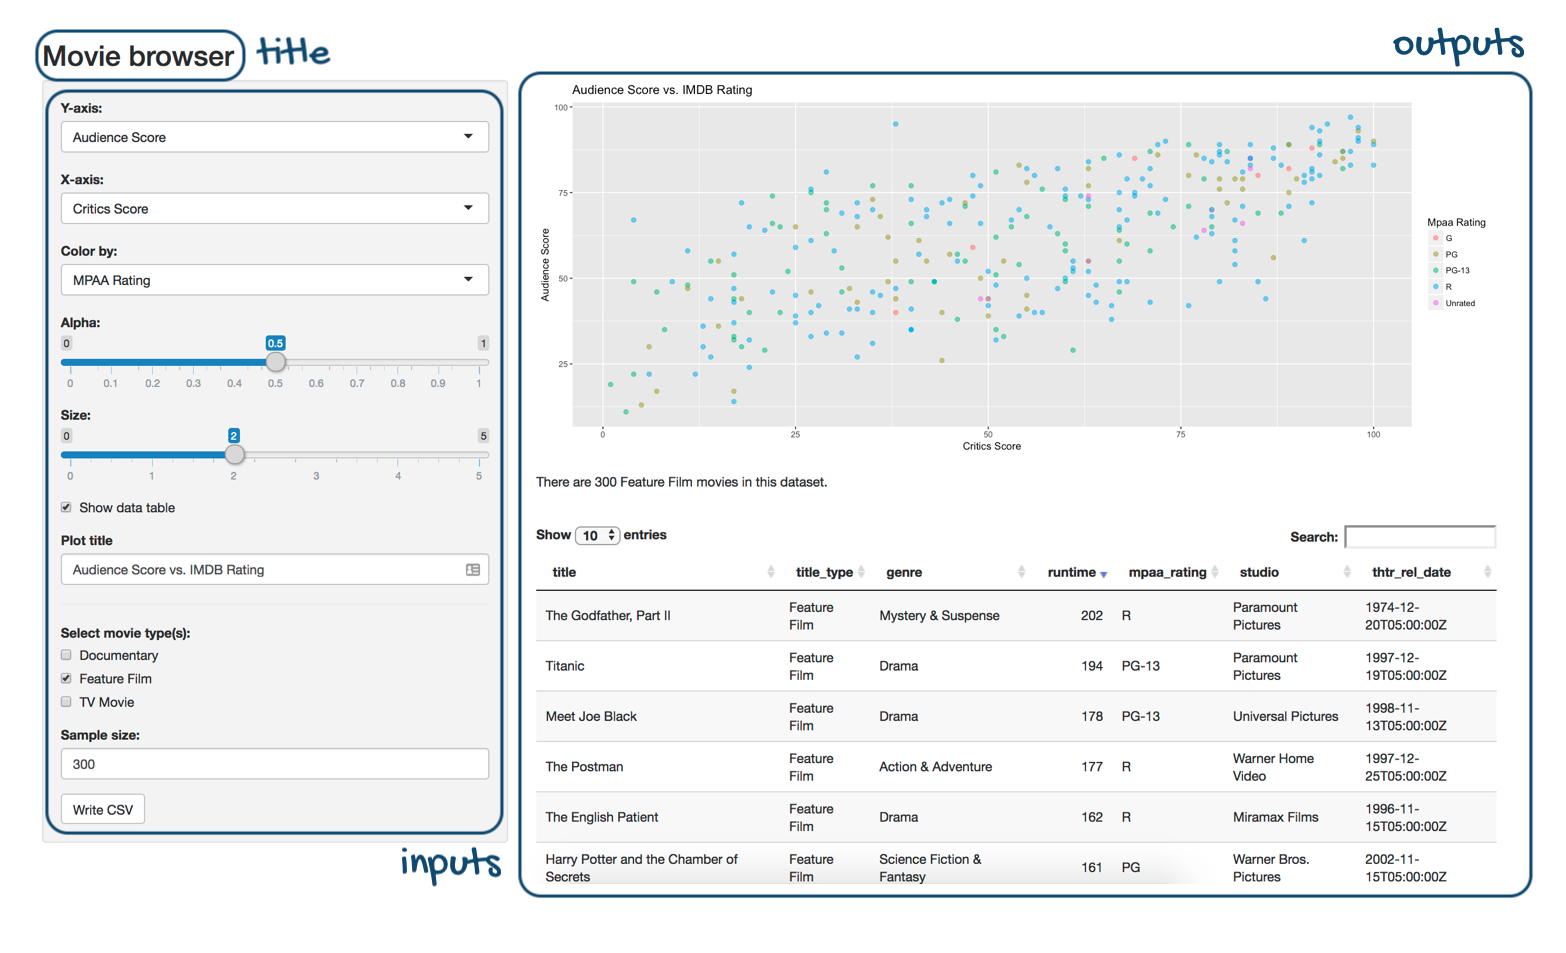
\includegraphics[width=1\textwidth,height=\textheight]{./images/shiny-app-annotated.png}

}

\end{figure}

We have:

\begin{itemize}
\tightlist
\item
  a title for the app,
\item
  a series of inputs:

  \begin{itemize}
  \tightlist
  \item
    some of these inputs use drop down menus for selection,
  \item
    some are sliders,
  \item
    some allow for text input, and
  \item
    some are action buttons
  \end{itemize}
\item
  and a few outputs:

  \begin{itemize}
  \tightlist
  \item
    a plot output that the user can interactively update,
  \item
    a text output that updates alongside it, and
  \item
    a data table output that also updates alongside these.
  \end{itemize}
\end{itemize}

As much as it looks like there is a lot going on in this sample app, the
app doesn't even scratch the surface of what you can build with Shiny.

I hope you're excited to take it all in!

\hypertarget{background}{%
\section{Background}\label{background}}

Before we get started with Shiny, let's talk background\ldots{}

This tutorial assumes that you are familiar with R as a programming
language.

Additionally, this tutorial uses packages from the
\href{https://tidyverse.org/}{tidyverse}
(e.g.~\href{https://dplyr.tidyverse.org/}{\textbf{dplyr}} for data
wrangling and \href{https://ggplot2.tidyverse.org/}{\textbf{ggplot2}}
for data visualisation). Your Shiny apps can use any package, but if
you'd like to learn more about doing data science with the tidyverse,
see \href{https://www.tidyverse.org/learn/}{here}.

\hypertarget{help}{%
\section{Help}\label{help}}

The tutorial is designed for beginners and many of the exercises have
plenty of scaffolding to help you along the way.

That being said, there are a few other resources that might help your
learning.

\begin{figure}

{\centering 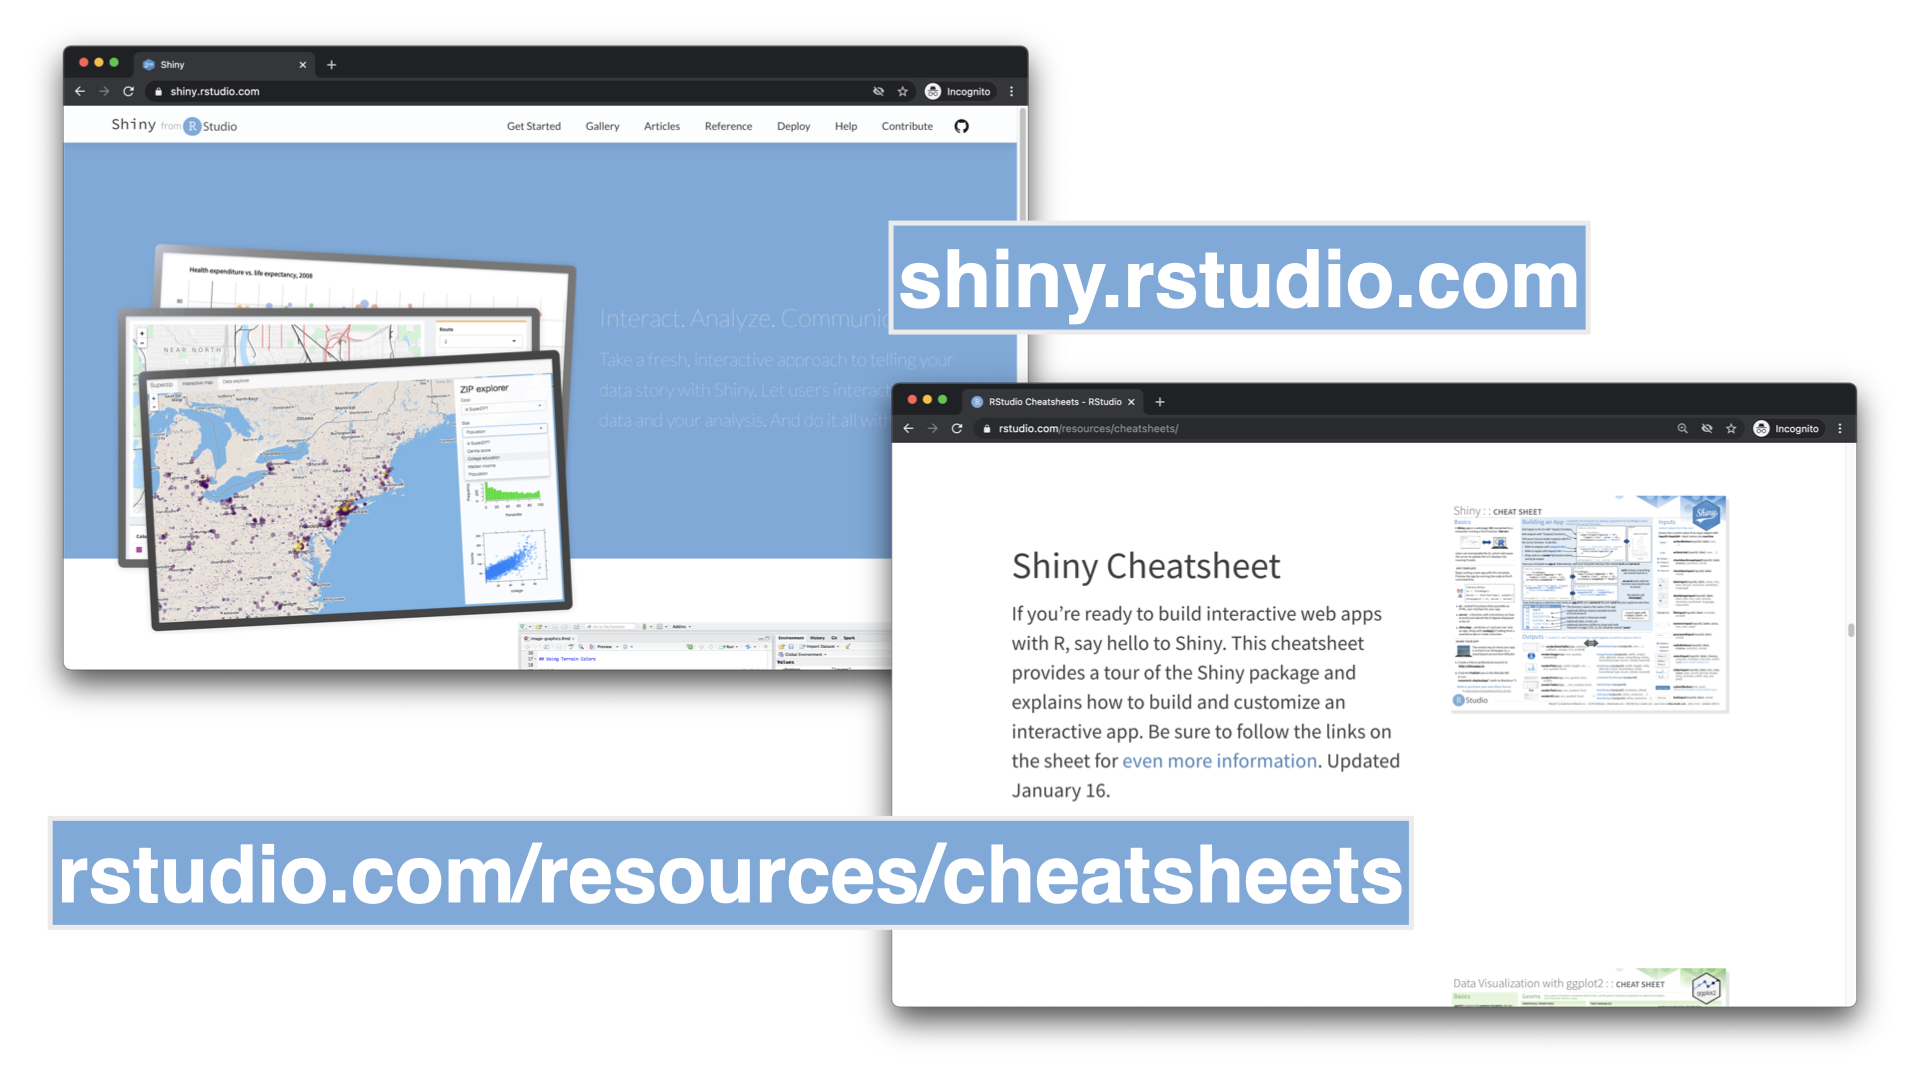
\includegraphics[width=0.8\textwidth,height=\textheight]{./images/help.png}

}

\end{figure}

\begin{enumerate}
\def\labelenumi{\arabic{enumi}.}
\item
  The first is the
  \href{https://github.com/rstudio/cheatsheets/raw/master/shiny.pdf}{\textbf{Shiny
  cheatsheet}}. This is a handy-dandy
  \href{https://rstudio.com/resources/cheatsheets/}{cheatsheet} that I
  recommend you keep close by when building Shiny apps.
\item
  The second is the \href{https://shiny.rstudio.com}{\textbf{Shiny
  homepage}}. It is \emph{the} place to learn about all things Shiny and
  to keep up to date with it as it evolves.
\end{enumerate}

\hypertarget{tips}{%
\section{Tips}\label{tips}}

Also, let's go over three very important tips for learning to develop
Shiny apps:

\begin{enumerate}
\def\labelenumi{\arabic{enumi}.}
\item
  Always \textbf{run the entire script} containing the R code, not just
  up to the point where you're developing code. For most exercises in
  this tutorial you will be asked to modify or update existing Shiny
  code, and even though you might be altering a small portion of the
  code, you still need to run the entire app code to create the app.
\item
  Sometimes the best way to troubleshoot is to \textbf{run the app and
  review the error}. Not only can the error message be informative, but
  googling the error message might quickly land you on a solution.
\item
  \textbf{Watch out for commas!} This will mean more as you start to
  learn Shiny, but just keep in mind, a Shiny error can often be caused
  by a missing comma. Thankfully, the RStudio IDE will alert you to most
  of these missing comma or similar syntax errors, like the one shown
  below.
\end{enumerate}

\begin{figure}

{\centering 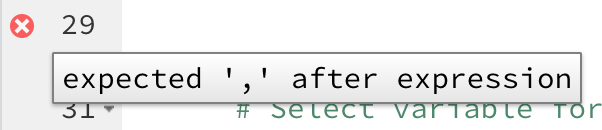
\includegraphics[width=0.3\textwidth,height=\textheight]{./images/missing-comma-ide.png}

}

\end{figure}

\hypertarget{anatomy-of-a-shiny-app}{%
\section{Anatomy of a Shiny app}\label{anatomy-of-a-shiny-app}}

Alrighty, let's take a look at the anatomy of a Shiny app:

\begin{figure}

{\centering 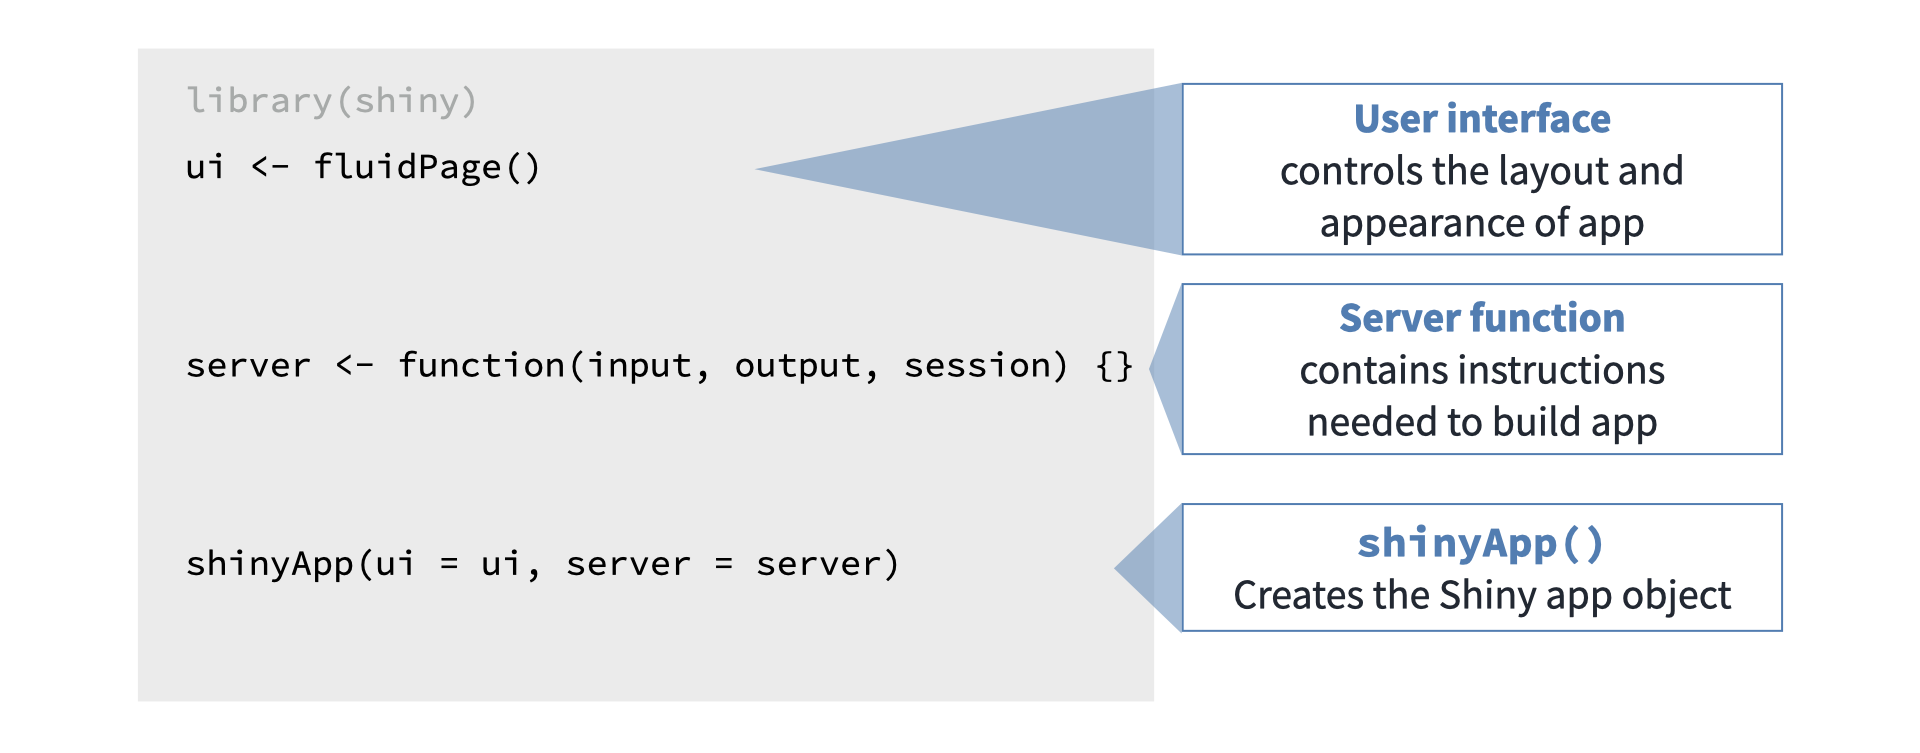
\includegraphics[width=0.8\textwidth,height=\textheight]{./images/anatomy.png}

}

\end{figure}

\begin{itemize}
\item
  We start by loading any necessary packages, one of which is
  necessarily shiny.
\item
  Then we lay out the user interface with a ui object that controls the
  appearance of our app.
\item
  And we define the server function that contains instructions needed to
  build the app.
\item
  We end each Shiny app script with a call to the shinyApp() function
  that puts these two components together to create the Shiny app
  object.
\end{itemize}

\hypertarget{data}{%
\section{Data}\label{data}}

In this tutorial we will build a simple movie browser app.

We will use data from the movies dataset, which combines data from two
websites: the Internet Movie Database, commonly known as IMDB, and
Rotten Tomatoes. The observations are a random sample of 651 movies
released in the US between 1970 and 2014.

So where does the loading of the data happen in an app?

\hypertarget{revisit}{%
\section{Revisit}\label{revisit}}

Let's revisit the app layout from a couple sections back.

\begin{figure}

{\centering 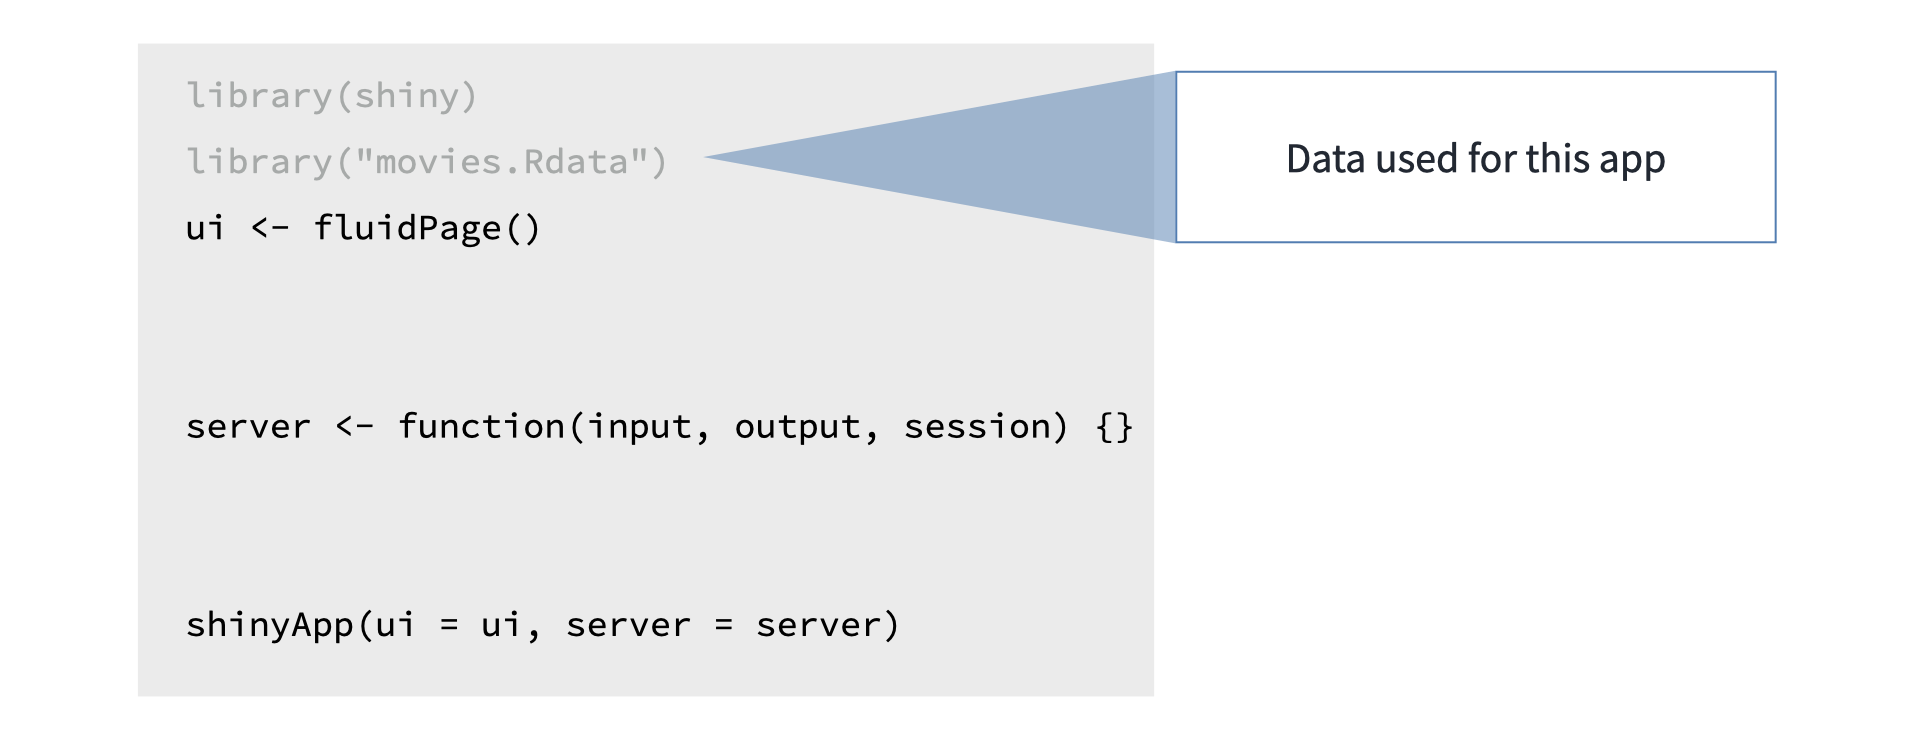
\includegraphics[width=0.8\textwidth,height=\textheight]{./images/revisit.png}

}

\end{figure}

We load the data before \texttt{ui} and \texttt{server} definitions so
that it can be used in both.

Alright, time for some practice!

\hypertarget{practice-whats-in-an-app}{%
\section{Practice: What's in an app?}\label{practice-whats-in-an-app}}

Which of these is not generally a part of the Shiny app architecture?''
- A function that installs an R package - User interface - Server
function - A function that creates Shiny app objects

Answer: A function that installs an R package. You don't want to
reinstall the package every time you run your app, so you should do this
once in your console instead of within your Shiny app

\hypertarget{practice-first-peek-under-the-hood}{%
\section{Practice: First peek under the
hood}\label{practice-first-peek-under-the-hood}}

Below you can see the complete code to reproduce the app we introduced
in the previous section. Now you get to interact with the app yourself,
and make small adjustments to it.

I've created an RStudio Cloud Project for you to test drive this code.
Click the button below to be taken to your RStudio Workspace, select
\textbf{1.1 First peek under the hood} from the Project list, and follow
the exercise instructions below to get started!

\emph{Navigate to the project called \textbf{1-1 First peek under the
hood} after clicking the button below}

\href{https://rstudio.cloud/spaces/81721/join?access_code=I4VJaNsKfTqR3Td9hLP7E1nz8\%2FtMg6Xbw9Bgqumv}{
Go to RStudio Cloud Workspace}

\hypertarget{your-turn}{%
\section{Your turn}\label{your-turn}}

\begin{itemize}
\tightlist
\item
  Once your RStudio Cloud Project is open to the script \texttt{app.R},
  click to run the code and generate the app.
\item
  Play with the input selectors for the Y-axis and the X-axis and
  observe how the output changes.
\item
  Close the app by closing the pop-up window or clicking on the red Stop
  button in the viewer.
\item
  Locate the relevant lines of code in \texttt{app.R} that build the
  selector widget for the Y-axis. This is in a \texttt{selectInput()}
  function starting on Line 20, underneath the comment
  \texttt{\#\ Select\ variable\ for\ y-axis}. Note that this function
  takes four arguments: \texttt{inputId}, \texttt{label},
  \texttt{choices}, and \texttt{selected}. We'll discuss what each of
  these mean in detail shortly. For now, change the \texttt{selected}
  argument to \texttt{imdb\_rating}, save your changes, and run the app
  again by clicking on . What changed?

  \begin{itemize}
  \tightlist
  \item
    If you get an error when you try to rerun the app, you can either
    try to debug the issue by tracing back your steps or delete
    everything in \texttt{app.R} and copy and paste the code below into
    \texttt{app.R}. This will get you back to your starting point. You
    can use this ``start over'' approach for any of the exercises in
    this tutorial.
  \end{itemize}
\item
  Now locate the relevant lines of code in \texttt{app.R} that build the
  selector widget for the X-axis. This is also in a
  \texttt{selectInput()} function, starting on Line 27, underneath the
  comment \texttt{\#\ Select\ variable\ for\ x-axis}. Change the
  \texttt{selected} argument to \texttt{imdb\_rating} as well, save your
  changes, and run the app again. What changed?
\end{itemize}

\begin{Shaded}
\begin{Highlighting}[]
\CommentTok{\# Load packages {-}{-}{-}{-}{-}{-}{-}{-}{-}{-}{-}{-}{-}{-}{-}{-}{-}{-}{-}{-}{-}{-}{-}{-}{-}{-}{-}{-}{-}{-}{-}{-}{-}{-}{-}{-}{-}{-}{-}{-}{-}{-}{-}{-}{-}{-}{-}{-}{-}{-}{-}{-}{-}{-}{-}{-}{-}{-}{-}{-}{-}{-}{-}{-}}

\FunctionTok{library}\NormalTok{(shiny)}
\FunctionTok{library}\NormalTok{(ggplot2)}

\CommentTok{\# Load data {-}{-}{-}{-}{-}{-}{-}{-}{-}{-}{-}{-}{-}{-}{-}{-}{-}{-}{-}{-}{-}{-}{-}{-}{-}{-}{-}{-}{-}{-}{-}{-}{-}{-}{-}{-}{-}{-}{-}{-}{-}{-}{-}{-}{-}{-}{-}{-}{-}{-}{-}{-}{-}{-}{-}{-}{-}{-}{-}{-}{-}{-}{-}{-}{-}{-}{-}{-}}

\FunctionTok{load}\NormalTok{(}\StringTok{"movies.RData"}\NormalTok{)}

\CommentTok{\# Define UI {-}{-}{-}{-}{-}{-}{-}{-}{-}{-}{-}{-}{-}{-}{-}{-}{-}{-}{-}{-}{-}{-}{-}{-}{-}{-}{-}{-}{-}{-}{-}{-}{-}{-}{-}{-}{-}{-}{-}{-}{-}{-}{-}{-}{-}{-}{-}{-}{-}{-}{-}{-}{-}{-}{-}{-}{-}{-}{-}{-}{-}{-}{-}{-}{-}{-}{-}{-}}

\NormalTok{ui }\OtherTok{\textless{}{-}} \FunctionTok{fluidPage}\NormalTok{(}

  \FunctionTok{sidebarLayout}\NormalTok{(}

    \CommentTok{\# Inputs: Select variables to plot}
    \FunctionTok{sidebarPanel}\NormalTok{(}

      \CommentTok{\# Select variable for y{-}axis}
      \FunctionTok{selectInput}\NormalTok{(}
        \AttributeTok{inputId =} \StringTok{"y"}\NormalTok{,}
        \AttributeTok{label =} \StringTok{"Y{-}axis:"}\NormalTok{,}
        \AttributeTok{choices =} \FunctionTok{c}\NormalTok{(}\StringTok{"imdb\_rating"}\NormalTok{, }\StringTok{"imdb\_num\_votes"}\NormalTok{, }\StringTok{"critics\_score"}\NormalTok{, }\StringTok{"audience\_score"}\NormalTok{, }\StringTok{"runtime"}\NormalTok{),}
        \AttributeTok{selected =} \StringTok{"audience\_score"}
\NormalTok{      ),}
      \CommentTok{\# Select variable for x{-}axis}
      \FunctionTok{selectInput}\NormalTok{(}
        \AttributeTok{inputId =} \StringTok{"x"}\NormalTok{,}
        \AttributeTok{label =} \StringTok{"X{-}axis:"}\NormalTok{,}
        \AttributeTok{choices =} \FunctionTok{c}\NormalTok{(}\StringTok{"imdb\_rating"}\NormalTok{, }\StringTok{"imdb\_num\_votes"}\NormalTok{, }\StringTok{"critics\_score"}\NormalTok{, }\StringTok{"audience\_score"}\NormalTok{, }\StringTok{"runtime"}\NormalTok{),}
        \AttributeTok{selected =} \StringTok{"critics\_score"}
\NormalTok{      )}
\NormalTok{    ),}

    \CommentTok{\# Output: Show scatterplot}
    \FunctionTok{mainPanel}\NormalTok{(}
      \FunctionTok{plotOutput}\NormalTok{(}\AttributeTok{outputId =} \StringTok{"scatterplot"}\NormalTok{)}
\NormalTok{    )}
\NormalTok{  )}
\NormalTok{)}

\CommentTok{\# Define server {-}{-}{-}{-}{-}{-}{-}{-}{-}{-}{-}{-}{-}{-}{-}{-}{-}{-}{-}{-}{-}{-}{-}{-}{-}{-}{-}{-}{-}{-}{-}{-}{-}{-}{-}{-}{-}{-}{-}{-}{-}{-}{-}{-}{-}{-}{-}{-}{-}{-}{-}{-}{-}{-}{-}{-}{-}{-}{-}{-}{-}{-}{-}{-}}

\NormalTok{server }\OtherTok{\textless{}{-}} \ControlFlowTok{function}\NormalTok{(input, output, session) \{}
\NormalTok{  output}\SpecialCharTok{$}\NormalTok{scatterplot }\OtherTok{\textless{}{-}} \FunctionTok{renderPlot}\NormalTok{(\{}
    \FunctionTok{ggplot}\NormalTok{(}\AttributeTok{data =}\NormalTok{ movies, }\FunctionTok{aes\_string}\NormalTok{(}\AttributeTok{x =}\NormalTok{ input}\SpecialCharTok{$}\NormalTok{x, }\AttributeTok{y =}\NormalTok{ input}\SpecialCharTok{$}\NormalTok{y)) }\SpecialCharTok{+}
      \FunctionTok{geom\_point}\NormalTok{()}
\NormalTok{  \})}
\NormalTok{\}}

\CommentTok{\# Create a Shiny app object {-}{-}{-}{-}{-}{-}{-}{-}{-}{-}{-}{-}{-}{-}{-}{-}{-}{-}{-}{-}{-}{-}{-}{-}{-}{-}{-}{-}{-}{-}{-}{-}{-}{-}{-}{-}{-}{-}{-}{-}{-}{-}{-}{-}{-}{-}{-}{-}{-}{-}{-}{-}}

\FunctionTok{shinyApp}\NormalTok{(}\AttributeTok{ui =}\NormalTok{ ui, }\AttributeTok{server =}\NormalTok{ server)}
\end{Highlighting}
\end{Shaded}

\hypertarget{user-interface-ui}{%
\section{User interface (UI)}\label{user-interface-ui}}

\hypertarget{section}{%
\subsection{}\label{section}}

In this section we'll build the user interface of a simple app.

However, before we get into the weeds of building a user interface,
let's revisit the anatomy of a Shiny app.

\begin{figure}

{\centering 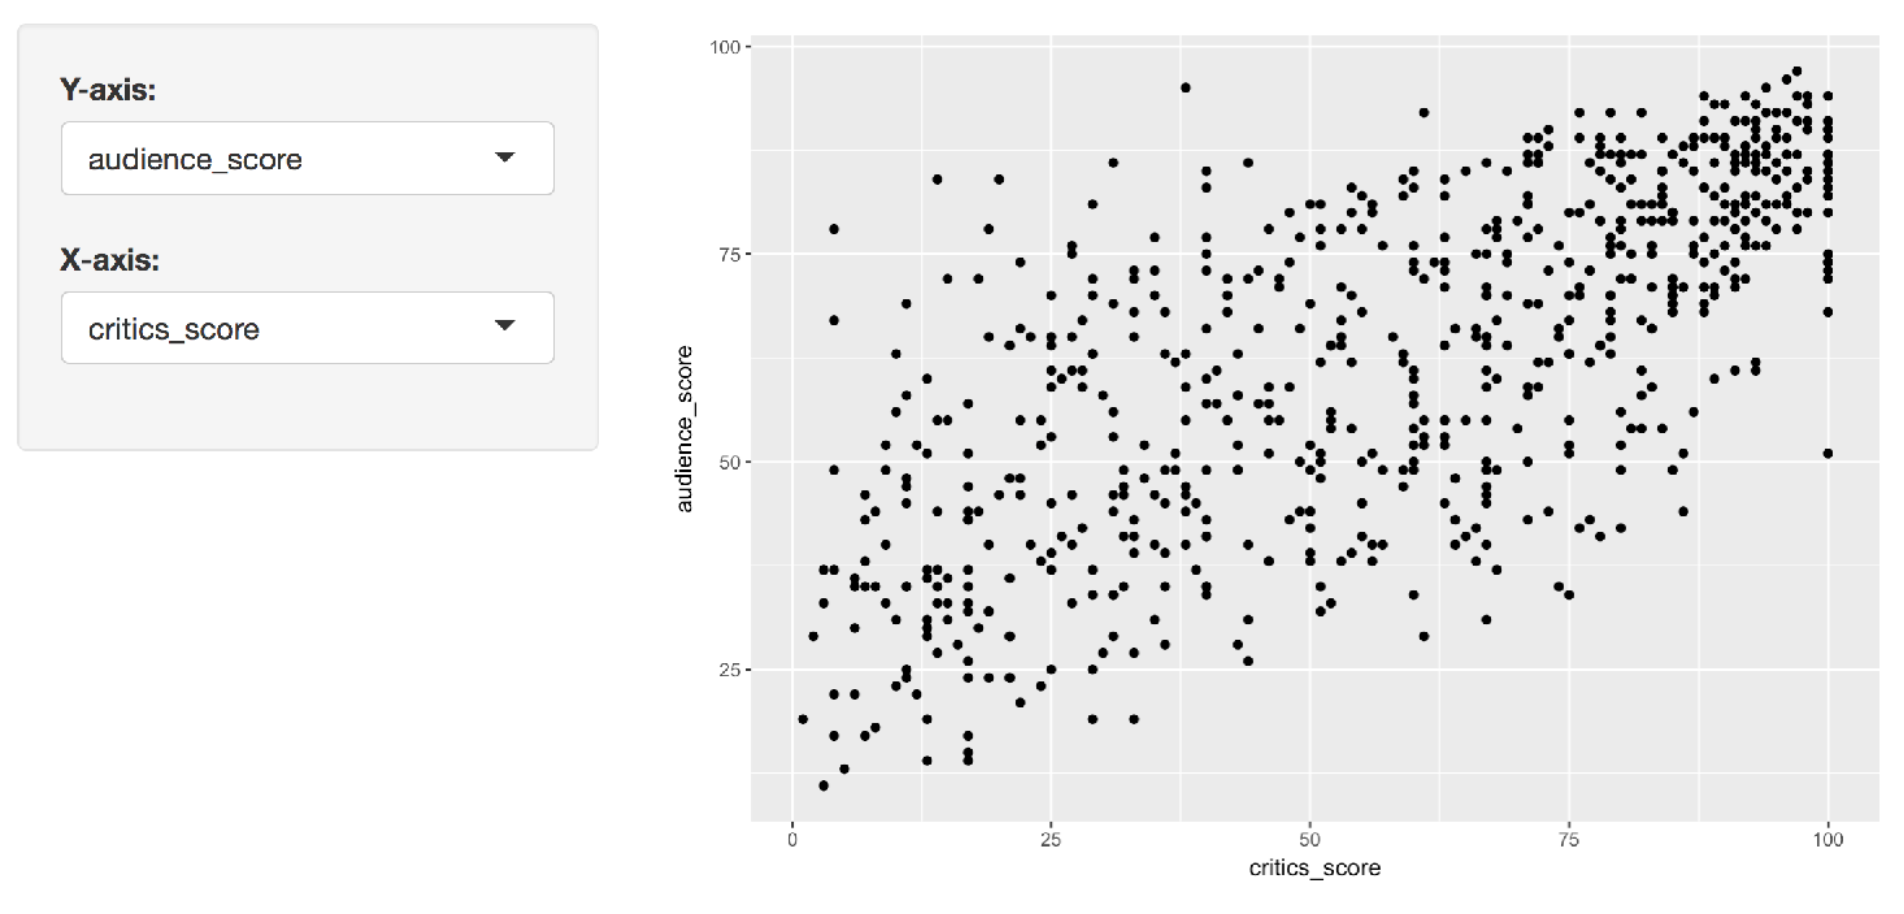
\includegraphics[width=1\textwidth,height=\textheight]{./images/app-selectinput-scatterplot.png}

}

\end{figure}

\begin{itemize}
\item
  The user interface, that we'll refer to as the ``UI'' going forward,
  defines and lays out the inputs of your app where users can make their
  selections. It also lays out the outputs.
\item
  The server function, on the other hand, calculates outputs and
  performs any other calculations needed for the outputs.
\end{itemize}

\hypertarget{example}{%
\subsection{Example}\label{example}}

\begin{figure}

{\centering 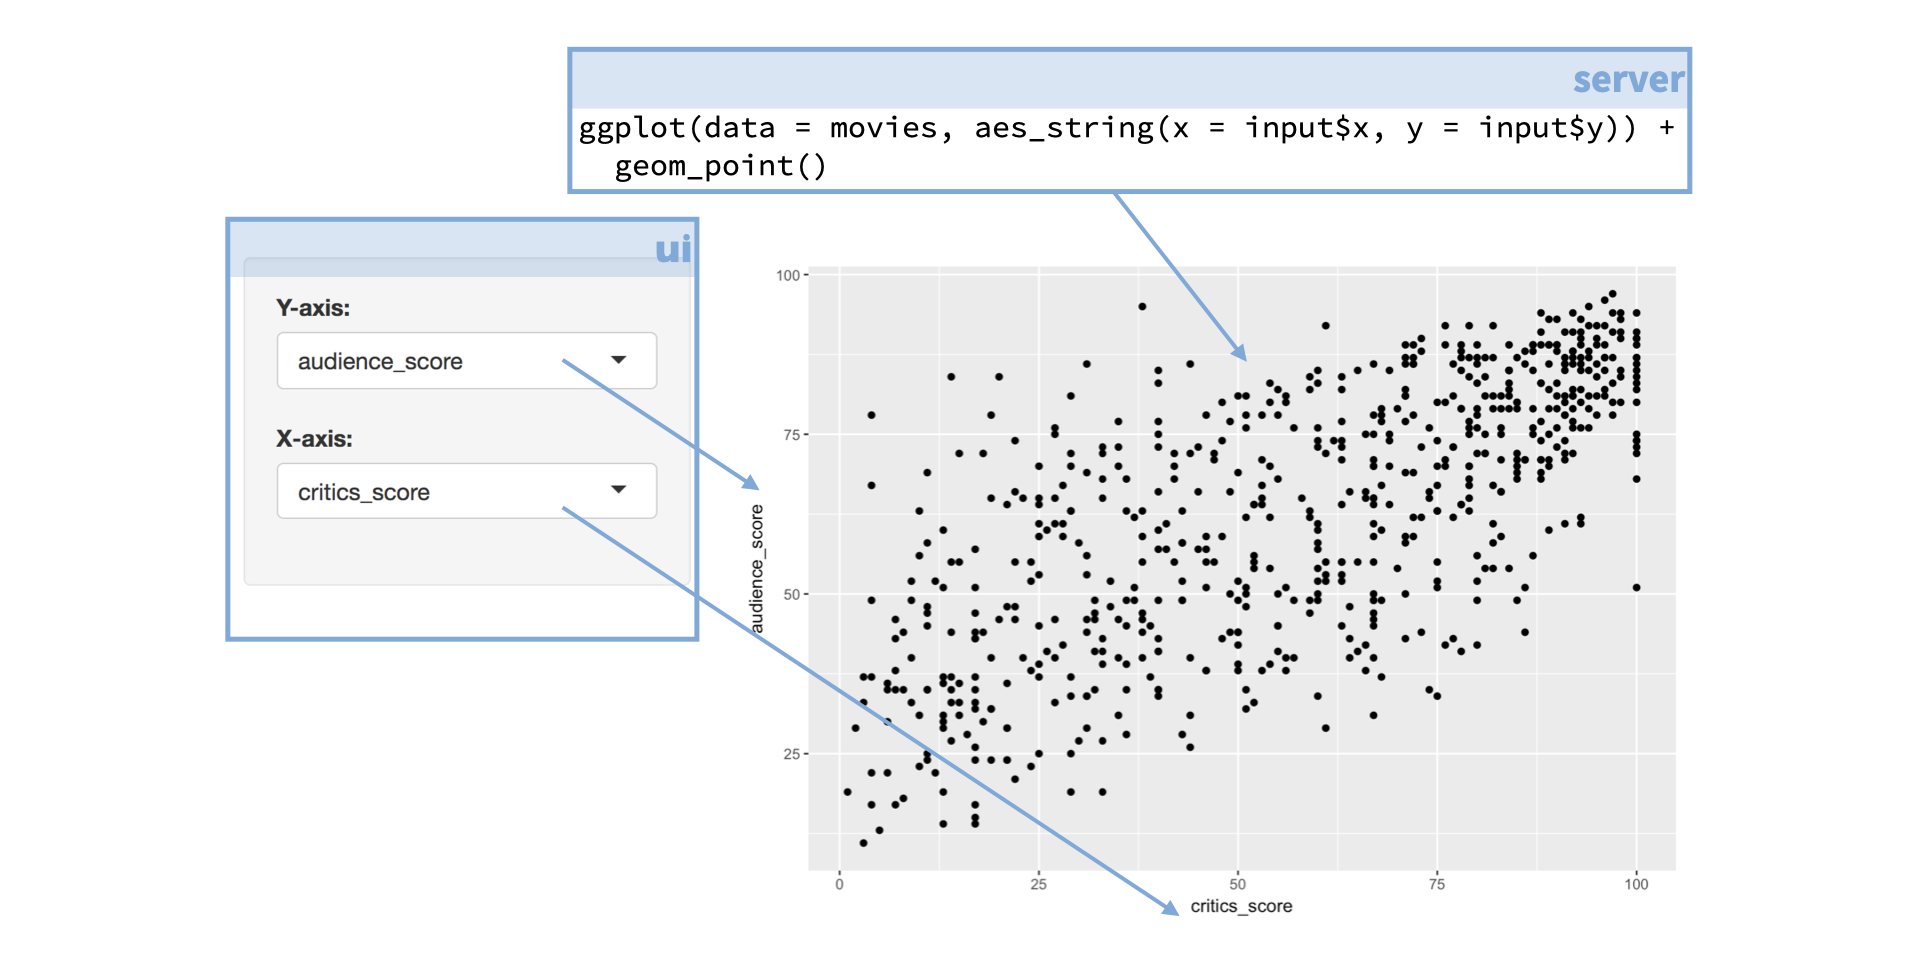
\includegraphics[width=1\textwidth,height=\textheight]{./images/ui-to-scatterplot.png}

}

\end{figure}

For example, if your app features a plot the code for building that plot
lives in the server function. But the setup for the user defined inputs
for the plot, as well as information on where physically on the app the
plot should appear, are defined in the UI.

\hypertarget{section-1}{%
\subsection{}\label{section-1}}

Here is the app we'll work with in this section and the code that builds
the UI of that app.

Since this is too much code to parse, we'll explore individual
components of the UI one by one.

\begin{figure}

{\centering 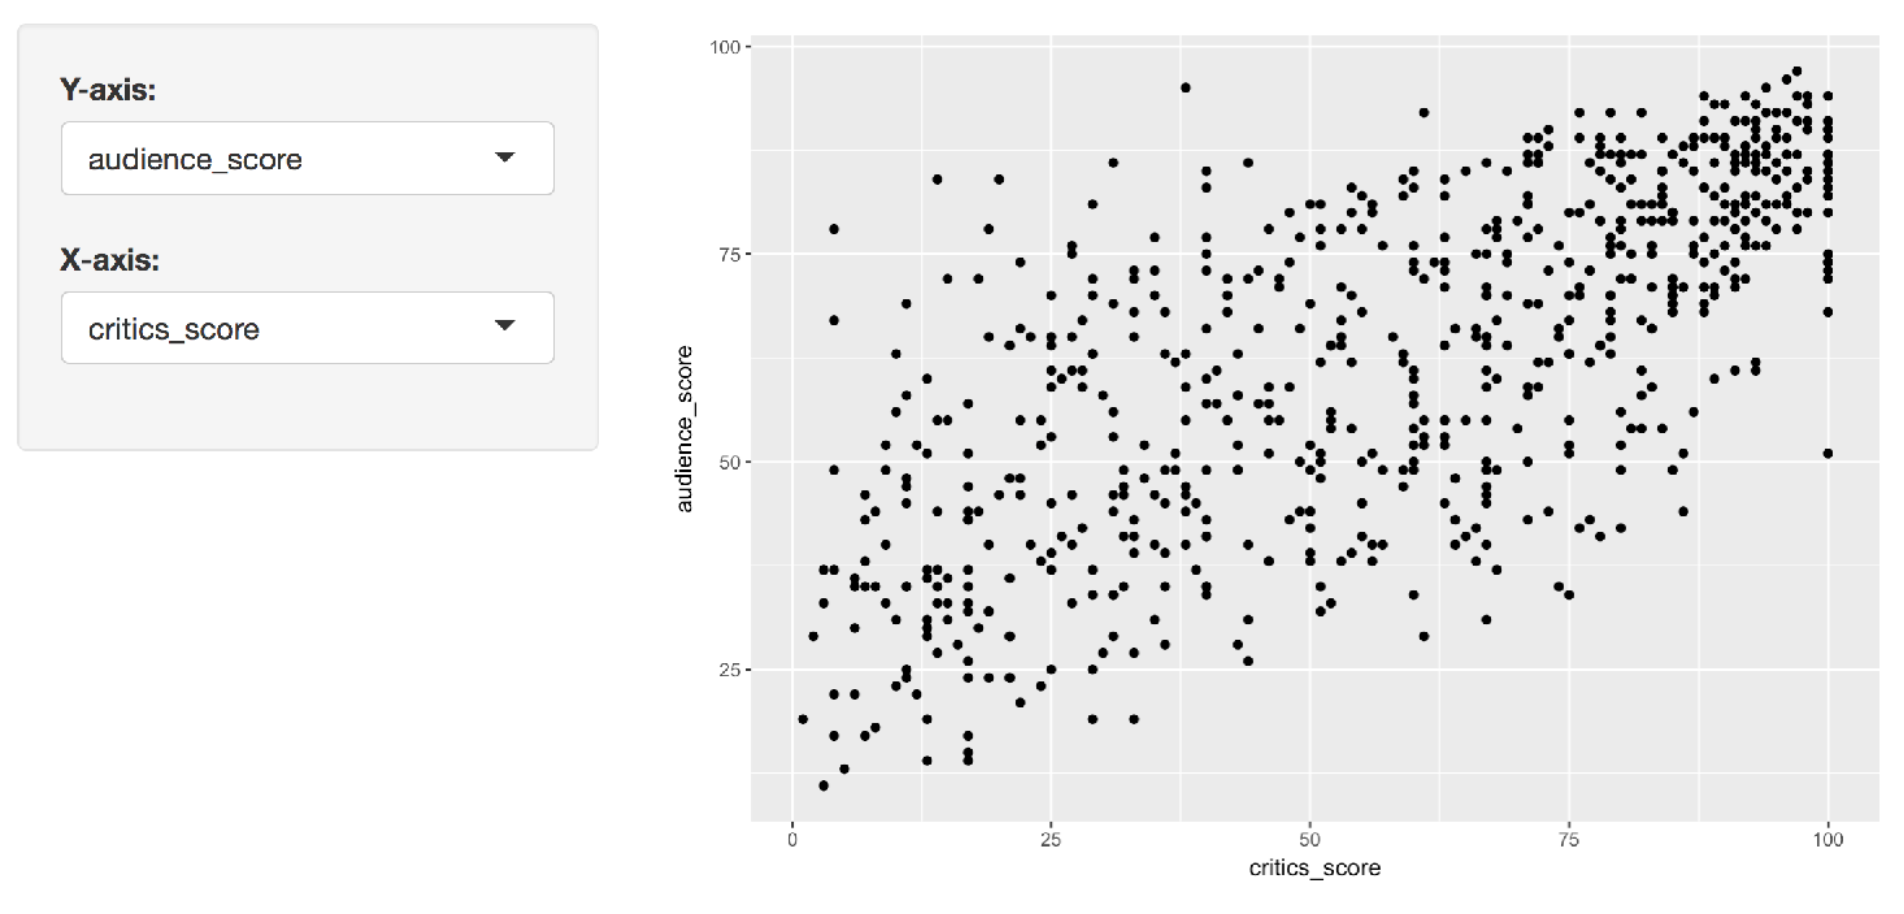
\includegraphics[width=1\textwidth,height=\textheight]{./images/app-selectinput-scatterplot.png}

}

\end{figure}

\begin{figure}

{\centering 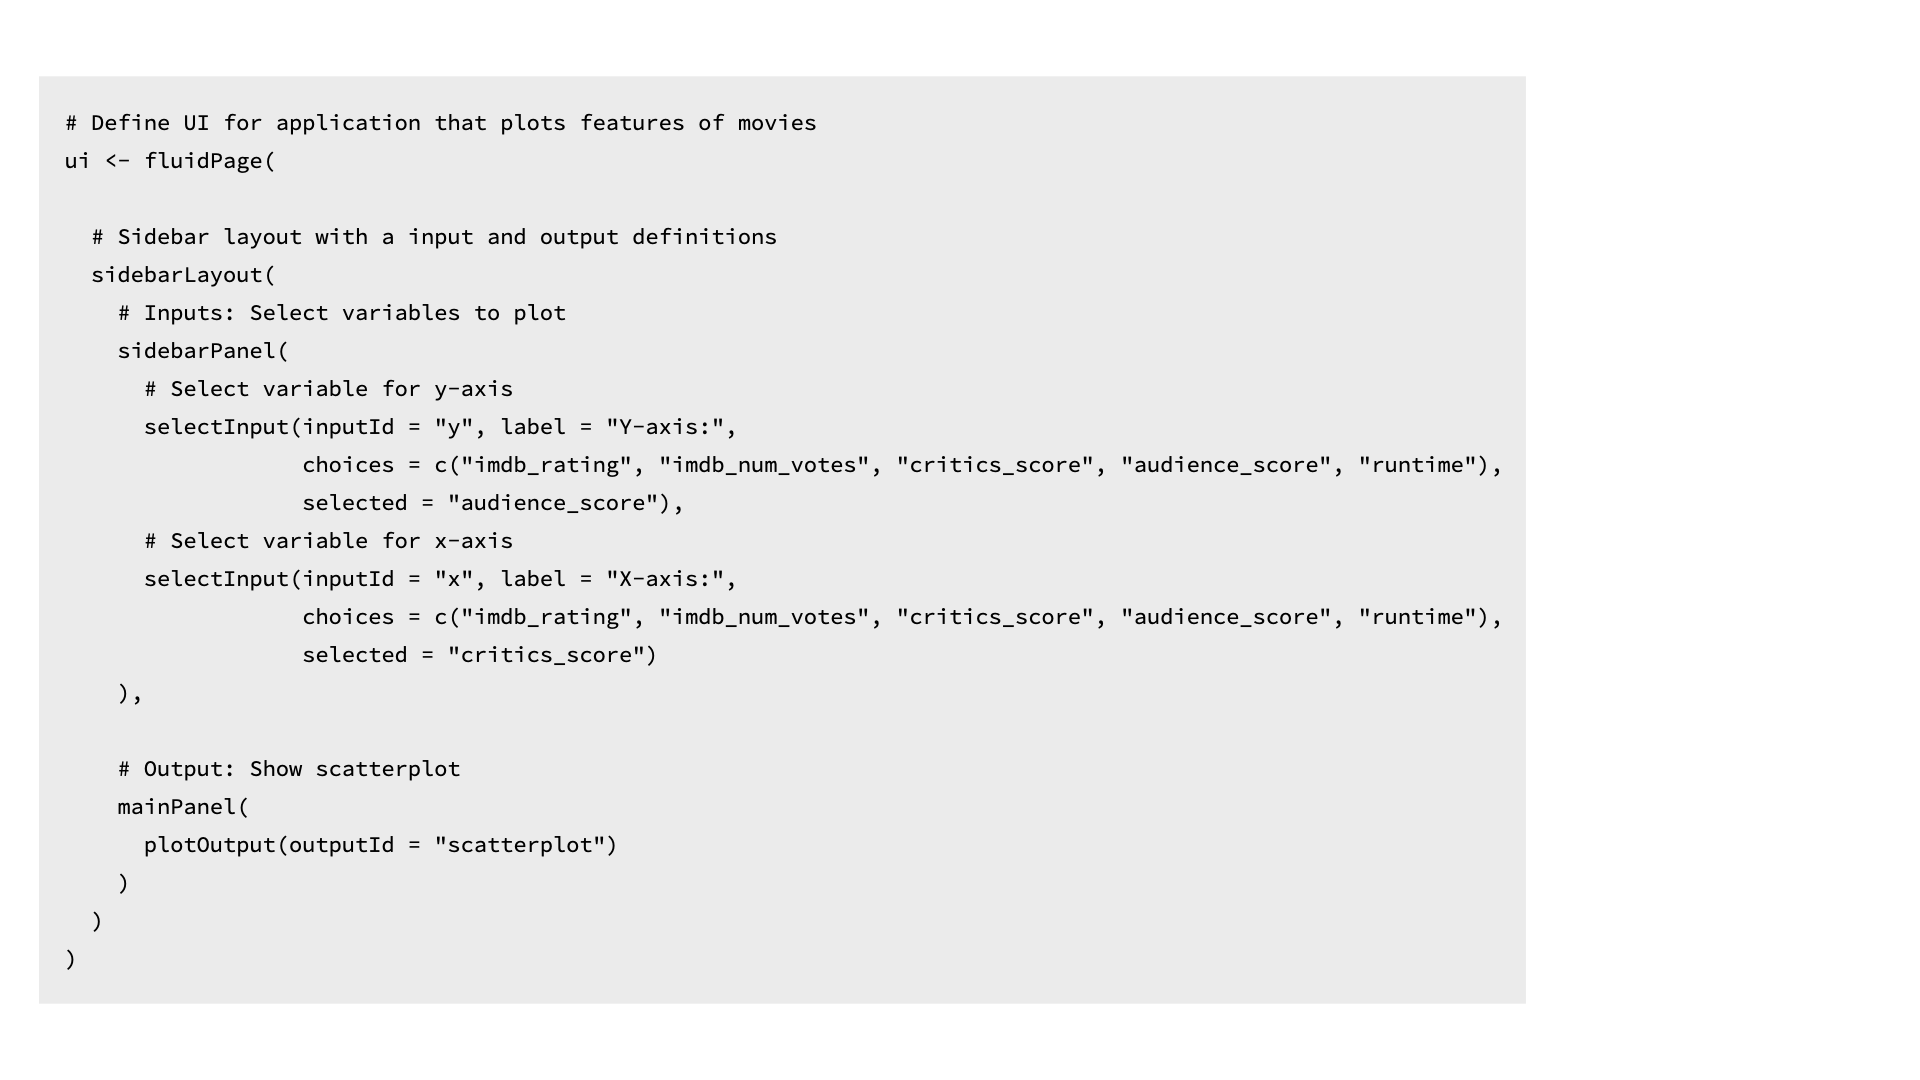
\includegraphics[width=1\textwidth,height=\textheight]{./images/ui-selectinput-scatterplot.png}

}

\end{figure}

\hypertarget{fluidpage}{%
\subsection{\texorpdfstring{\texttt{fluidPage()}}{fluidPage()}}\label{fluidpage}}

At the outermost layer of our UI definition we begin with the
\texttt{fluidPage()} function.

\begin{figure}

{\centering 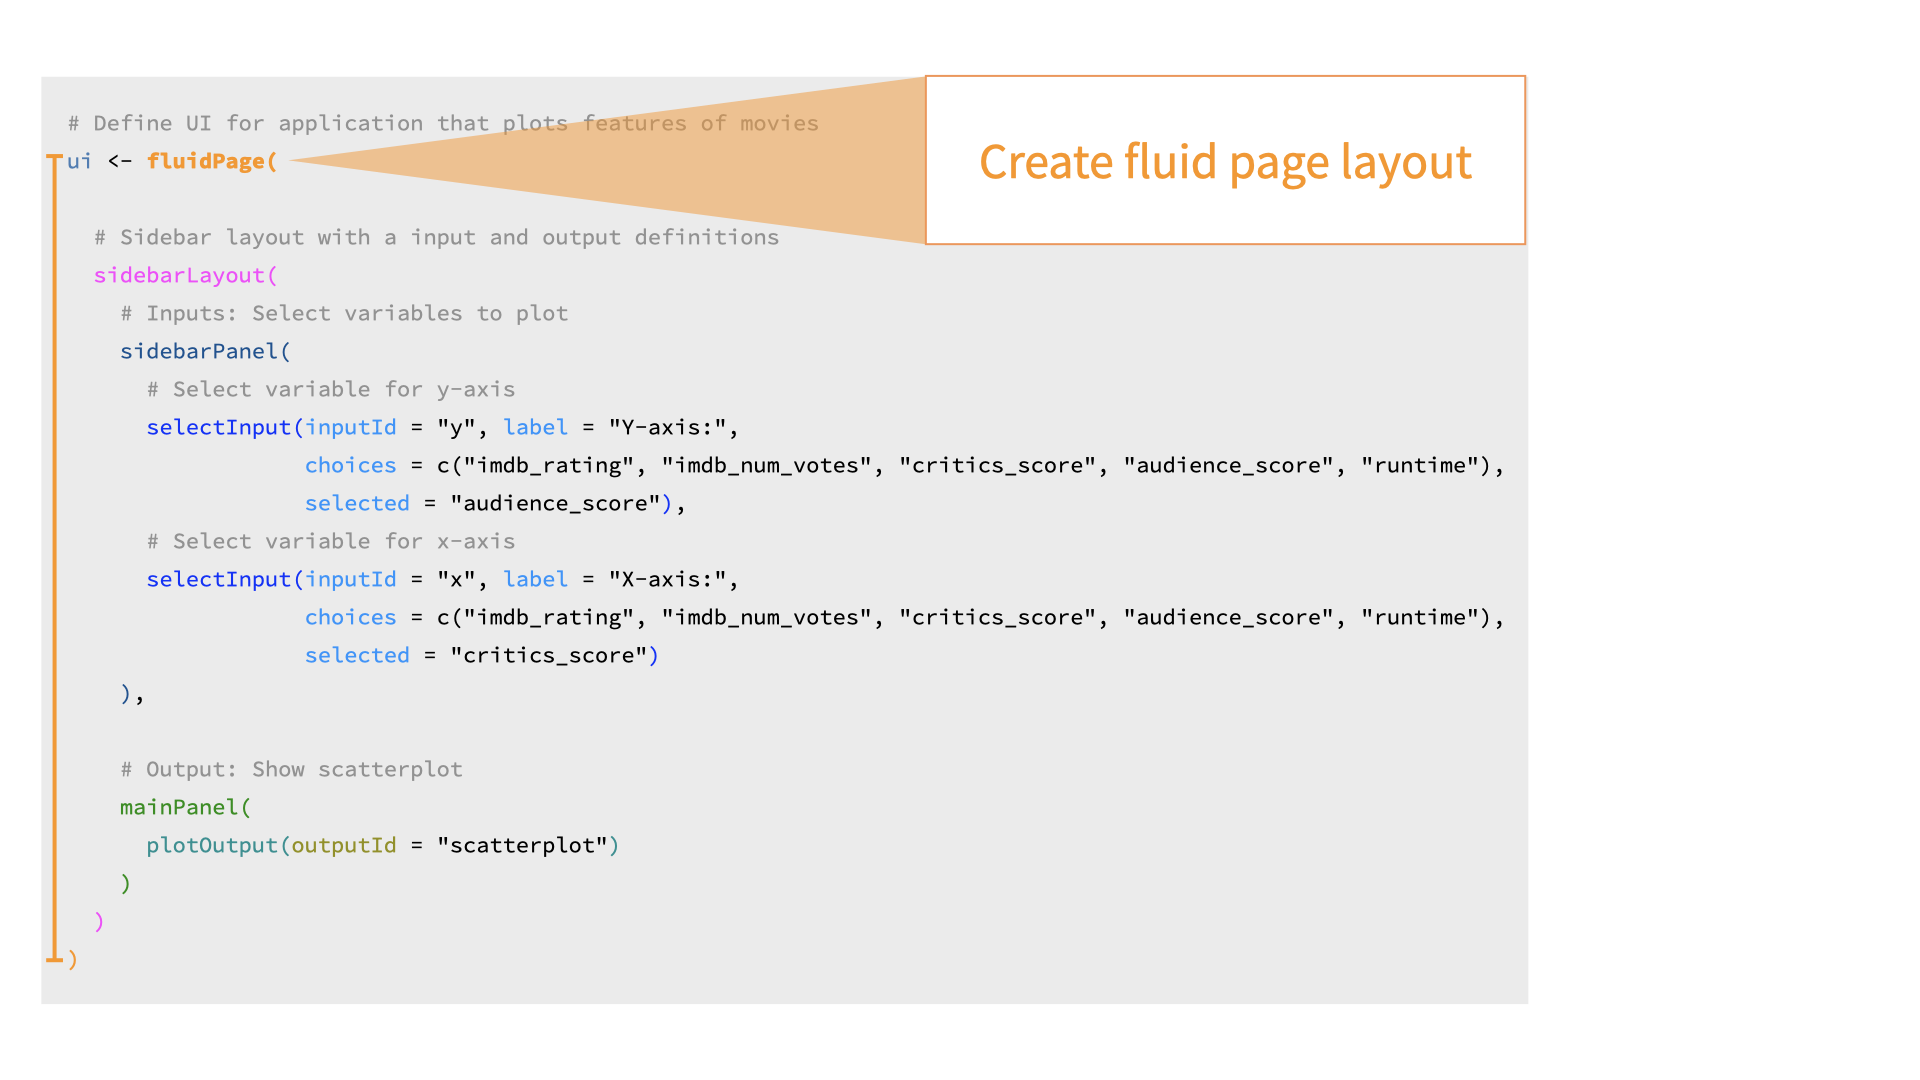
\includegraphics[width=1\textwidth,height=\textheight]{./images/fluidPage.png}

}

\end{figure}

The \texttt{fluidPage()} function creates a fluid page layout consisting
of rows and columns. Rows make sure that elements in them appear on the
same line. Columns within these rows define how much horizontal space
each element should occupy.

Fluid pages scale their components in realtime to fill all available
browser width, which means you, the app developer, don't need to worry
about defining relative widths for individual app components.

As always, for more information on arguments to this function, you can
view the R function help by typing \texttt{?fluidPage} in your R console
or visiting the function reference page on the package website
\href{https://shiny.rstudio.com/reference/shiny/latest/}{here}.

\hypertarget{layout}{%
\subsection{Layout}\label{layout}}

Next, we define the layout of our app with \texttt{sidebarLayout()}.

\begin{figure}

{\centering 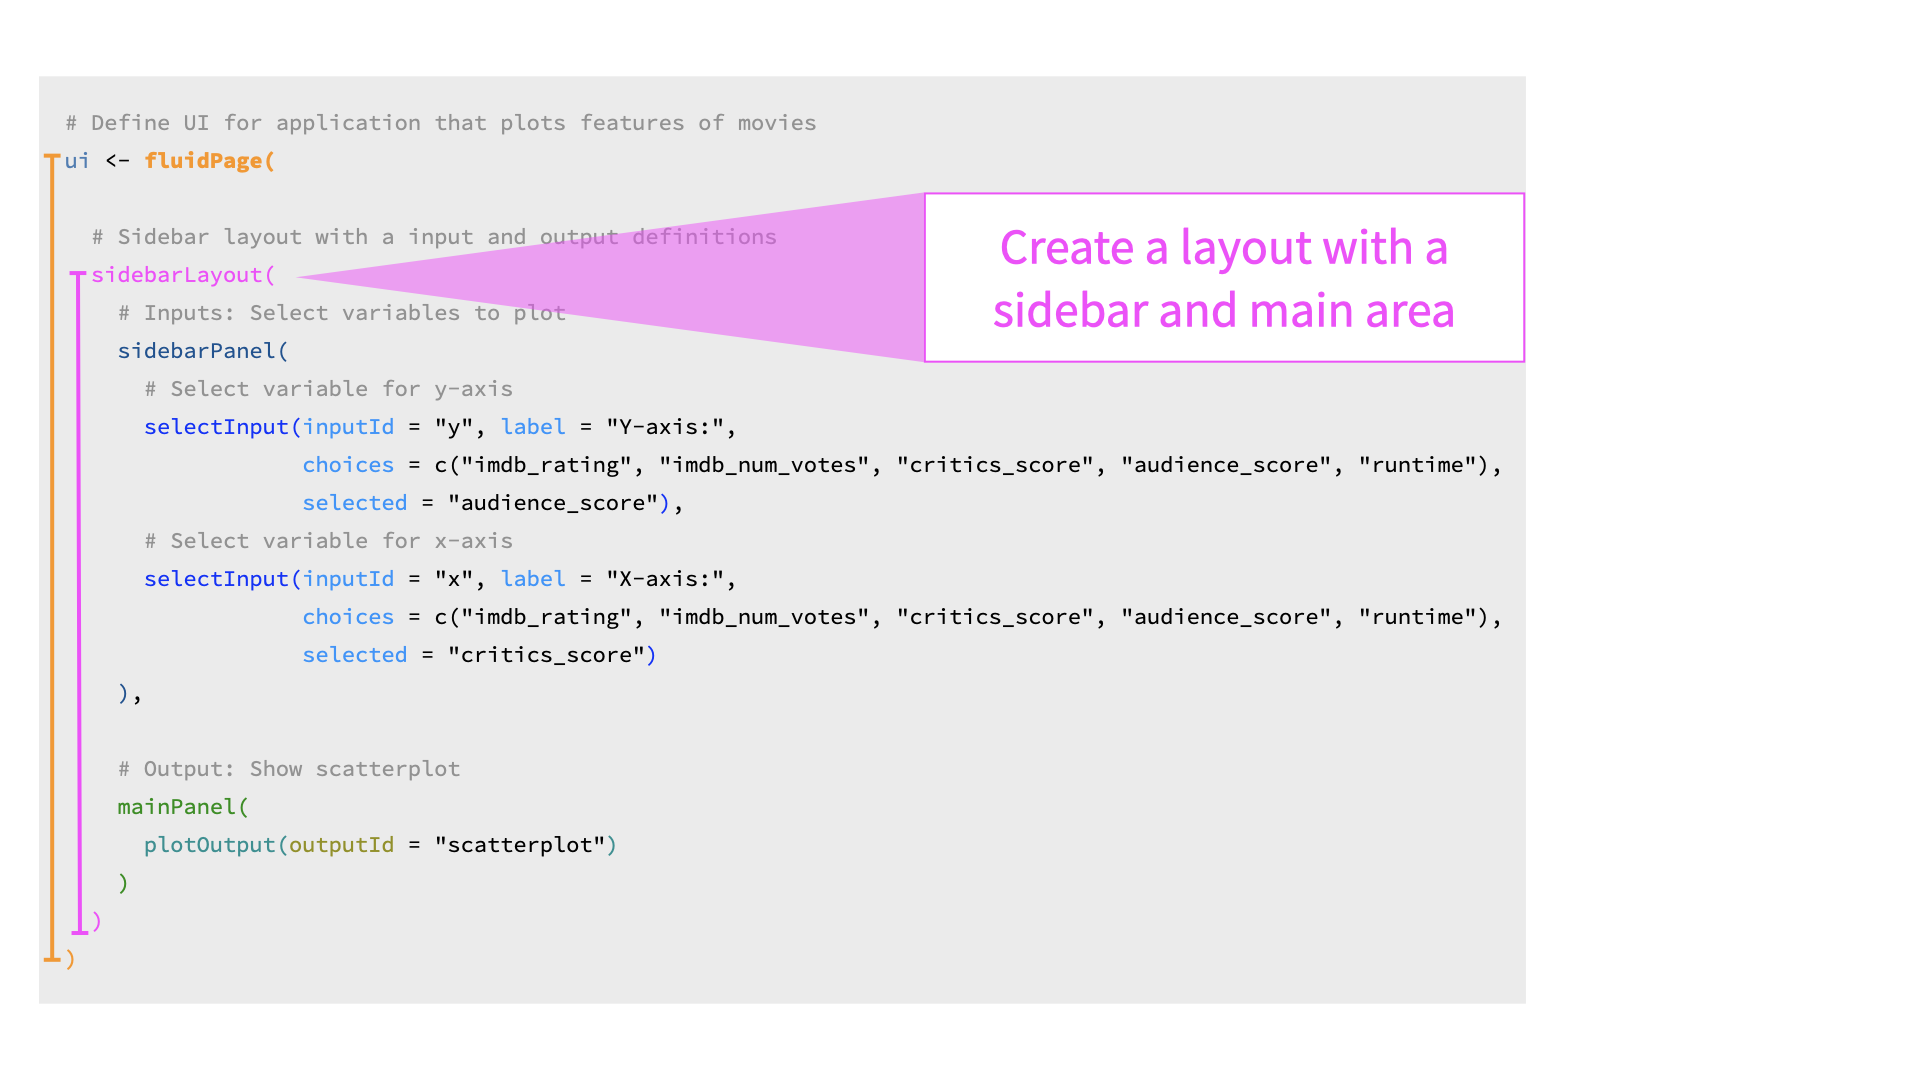
\includegraphics[width=1\textwidth,height=\textheight]{./images/layout.png}

}

\end{figure}

Shiny includes a number of options for laying out the components of an
application. The default layout, the one we're using in our example app,
is a layout with a sidebar, that you can define with the
\texttt{sidebarLayout()} function.

\begin{figure}

{\centering 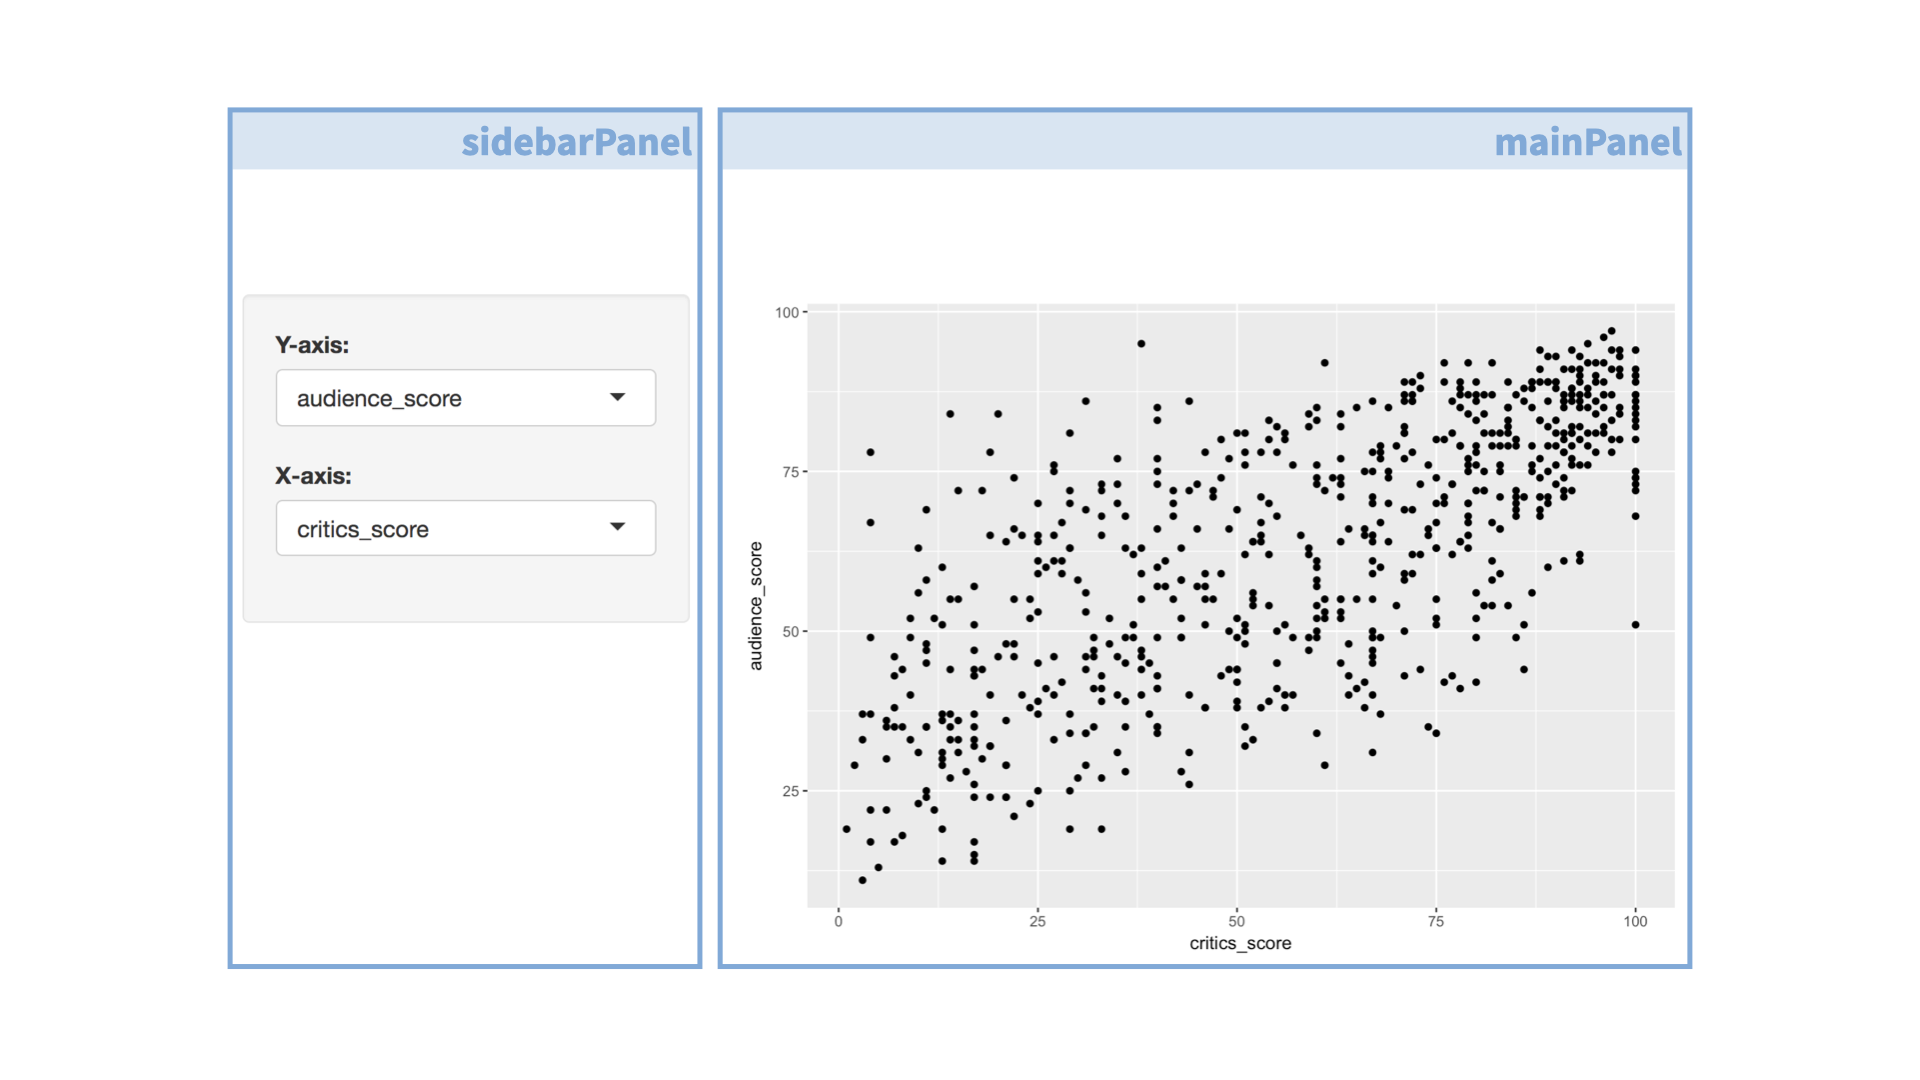
\includegraphics[width=1\textwidth,height=\textheight]{./images/layout-app.png}

}

\end{figure}

This is a simple layout with a narrow sidebar for inputs and a wider
main area for output.

Under the hood, Shiny implements layout features available in Bootstrap
2, which is a popular HTML/CSS framework. However the nice thing about
working in Shiny is that no prior experience with Bootstrap is
necessary.

To learn more about various layouts, I recommend reviewing the
\href{https://shiny.rstudio.com/articles/layout-guide.html}{Application
Layout Guide article} at \url{shiny.rstudio.com}.

\hypertarget{input-controls}{%
\subsection{Input controls}\label{input-controls}}

Next we define our sidebar panel containing input controls.

\begin{figure}

{\centering 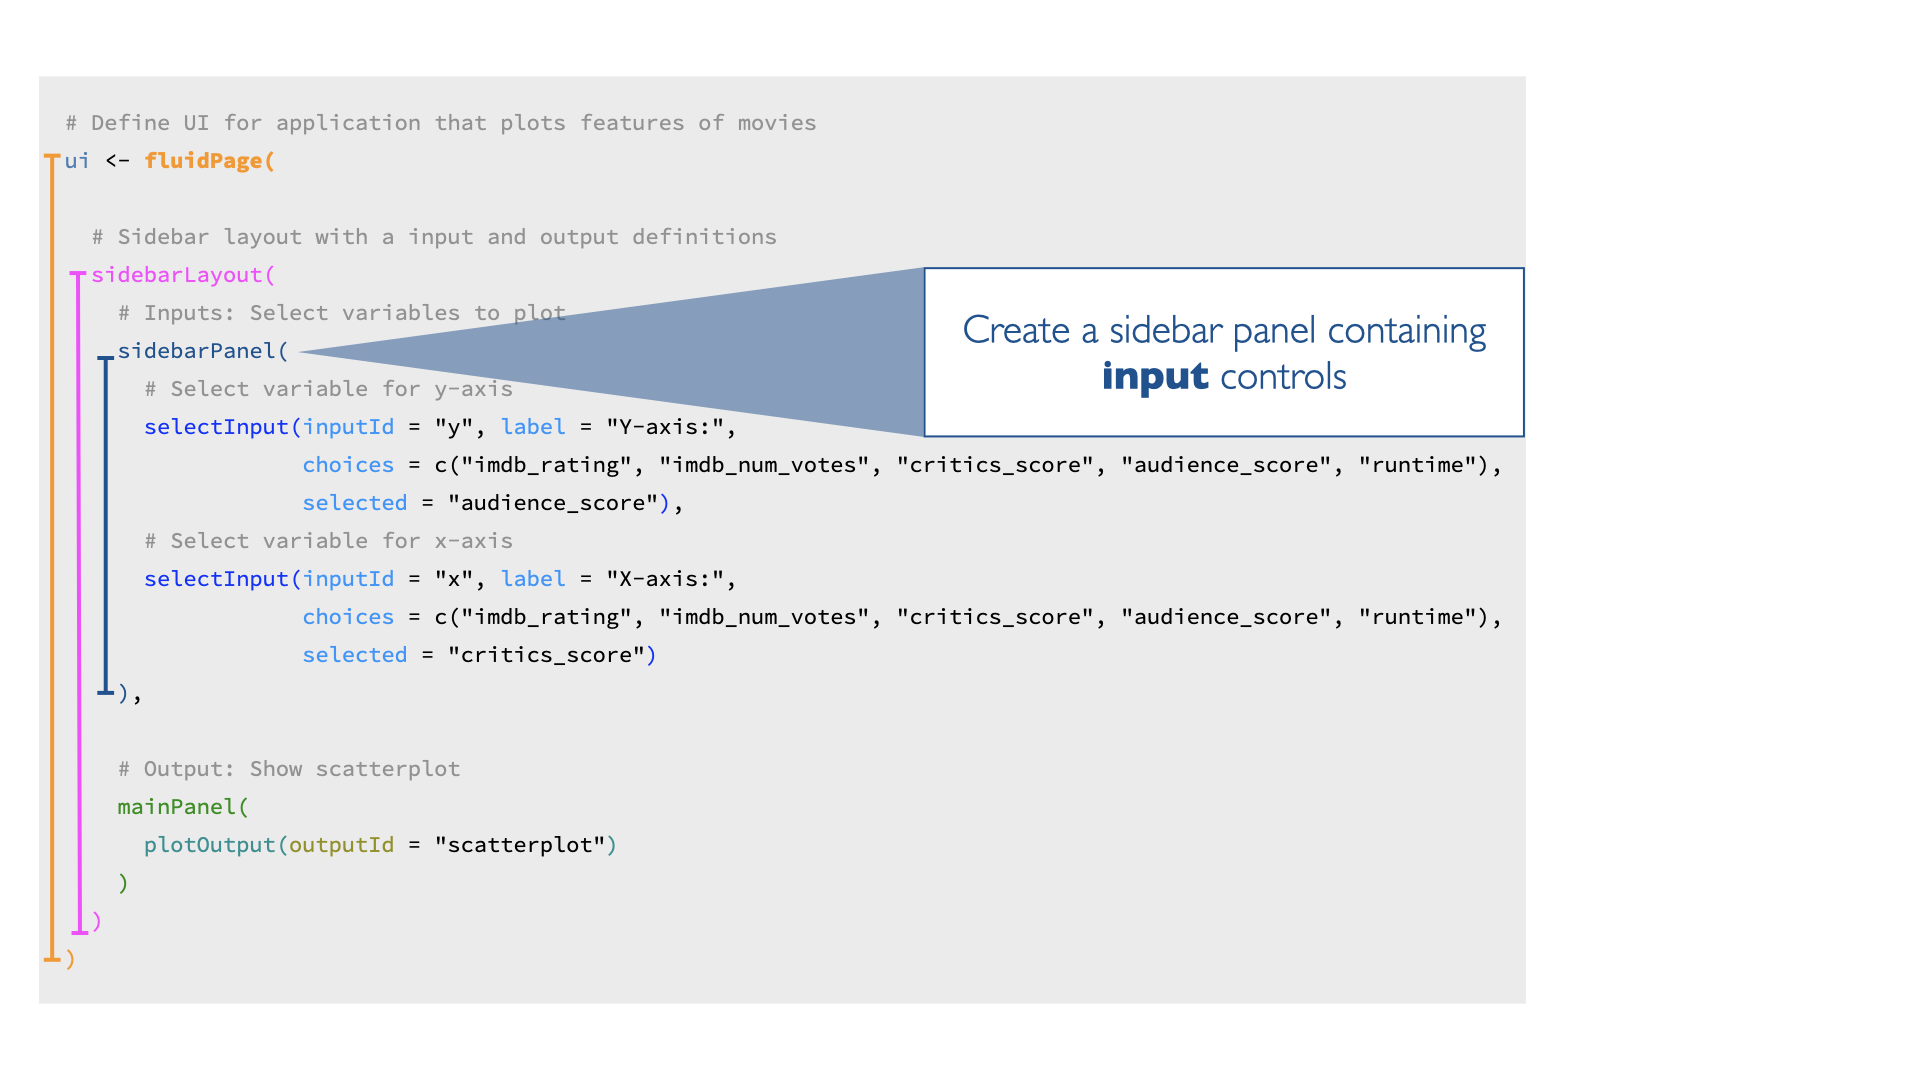
\includegraphics[width=1\textwidth,height=\textheight]{./images/input-controls.png}

}

\end{figure}

\hypertarget{section-2}{%
\subsection{}\label{section-2}}

This panel contains two dropdown menus created with the
\texttt{selectInput()} function.

\begin{figure}

{\centering 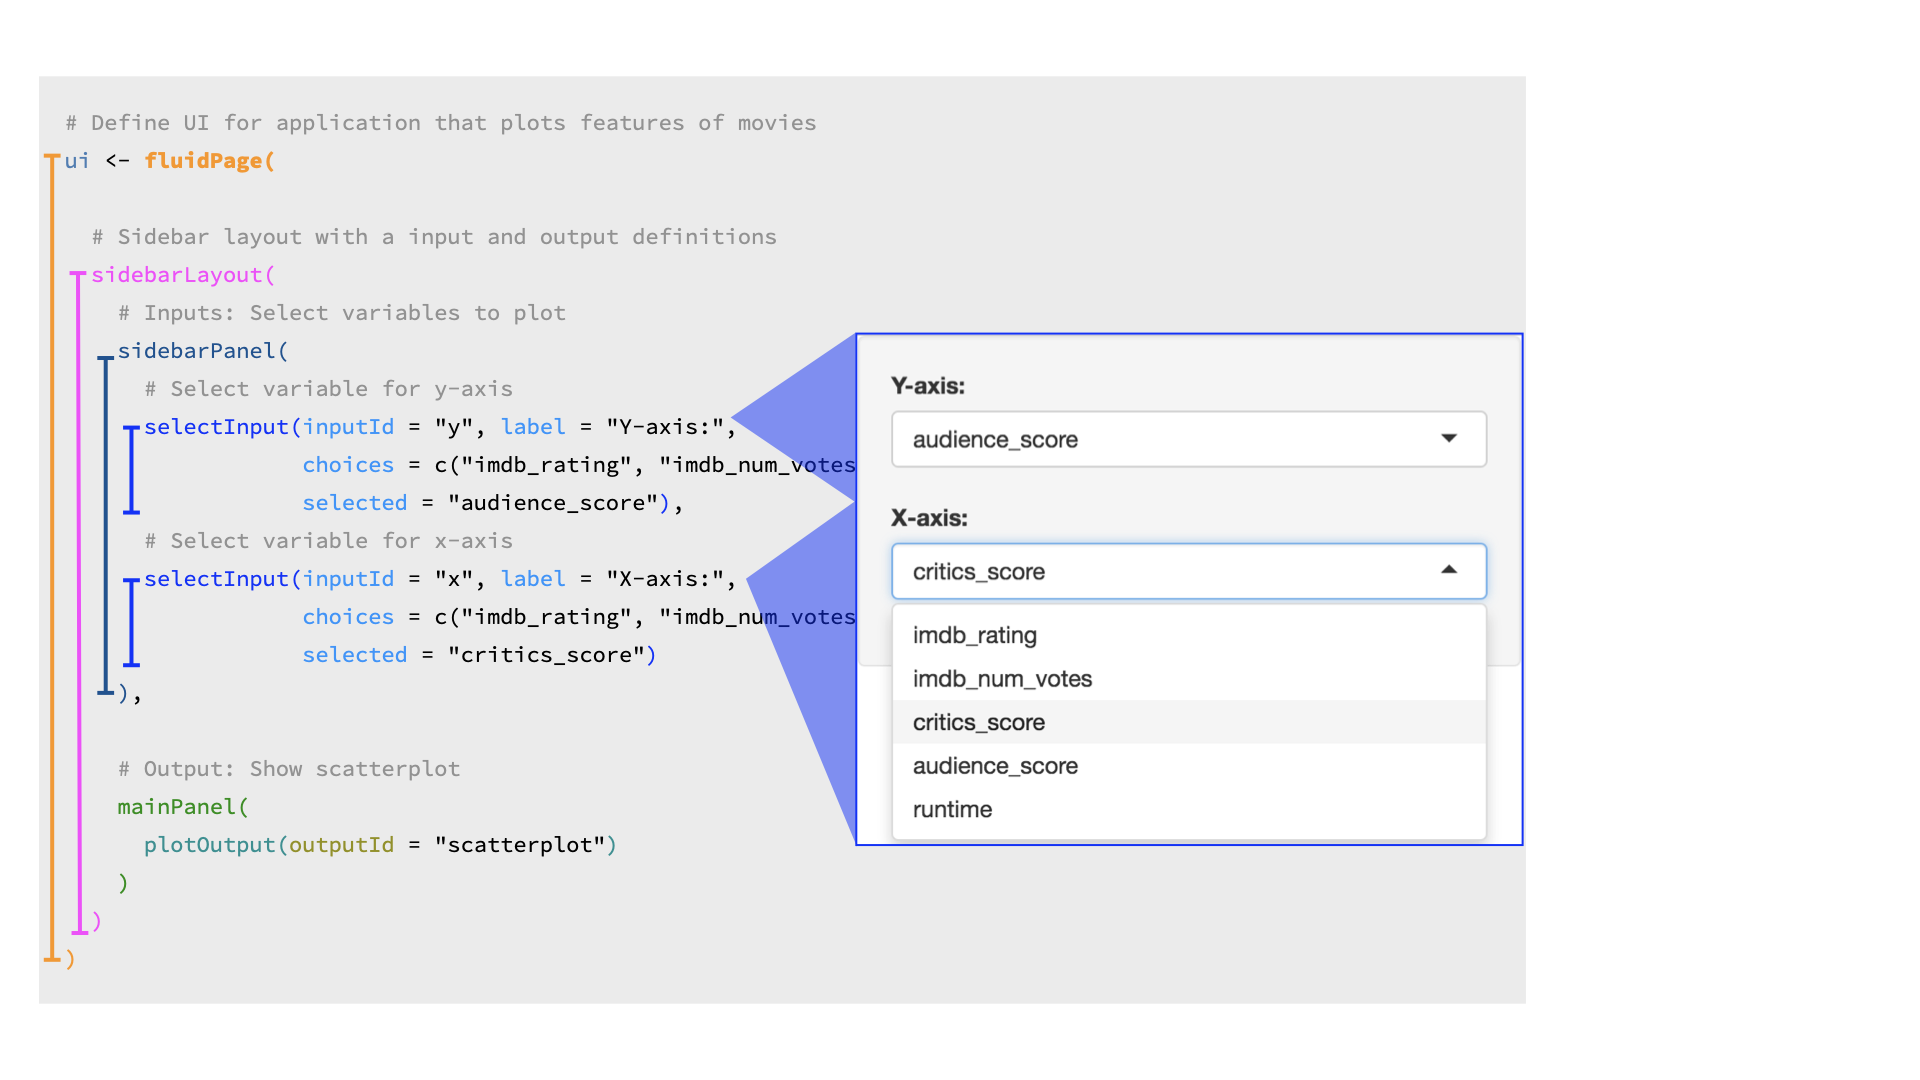
\includegraphics[width=1\textwidth,height=\textheight]{./images/input-dropdowns.png}

}

\end{figure}

\hypertarget{section-3}{%
\subsection{}\label{section-3}}

Let's take a look at one of the \texttt{selectInput} widgets a little
more closely.

\begin{figure}

{\centering 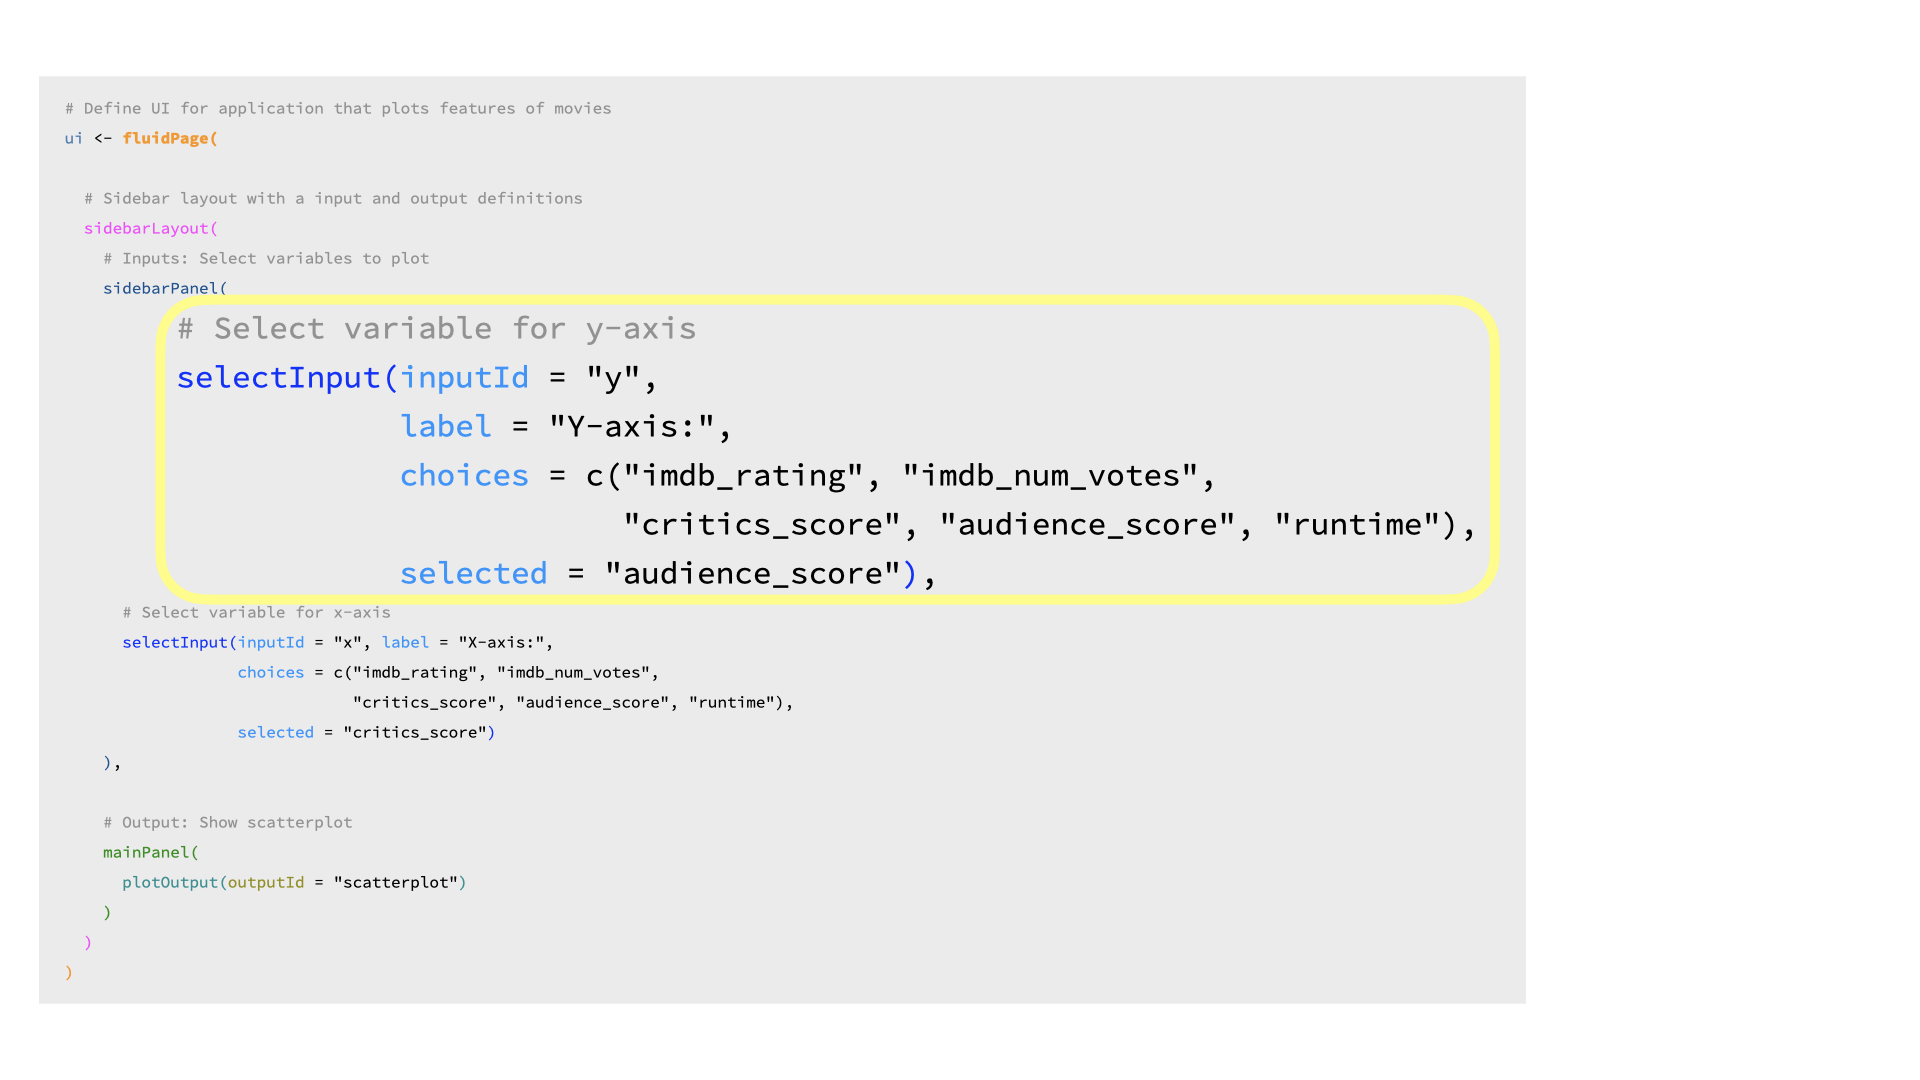
\includegraphics[width=1\textwidth,height=\textheight]{./images/input-closeup.png}

}

\end{figure}

\begin{enumerate}
\def\labelenumi{\arabic{enumi}.}
\item
  The first argument is the \texttt{inputId}, which is the input value
  that the app will internally use to access the value selected by the
  user.
\item
  The second argument is the \texttt{label}, which is the display label
  that the user sees.
\item
  The third argument is the list of \texttt{choices} the user will
  choose from. In this app, these are variable names from the movies
  dataset.
\item
  And lastly we specify a default selection from that list with
  \texttt{selected}.
\end{enumerate}

\hypertarget{main-panel}{%
\subsection{Main Panel}\label{main-panel}}

The final component of our UI is \texttt{mainPanel()}.

\begin{figure}

{\centering 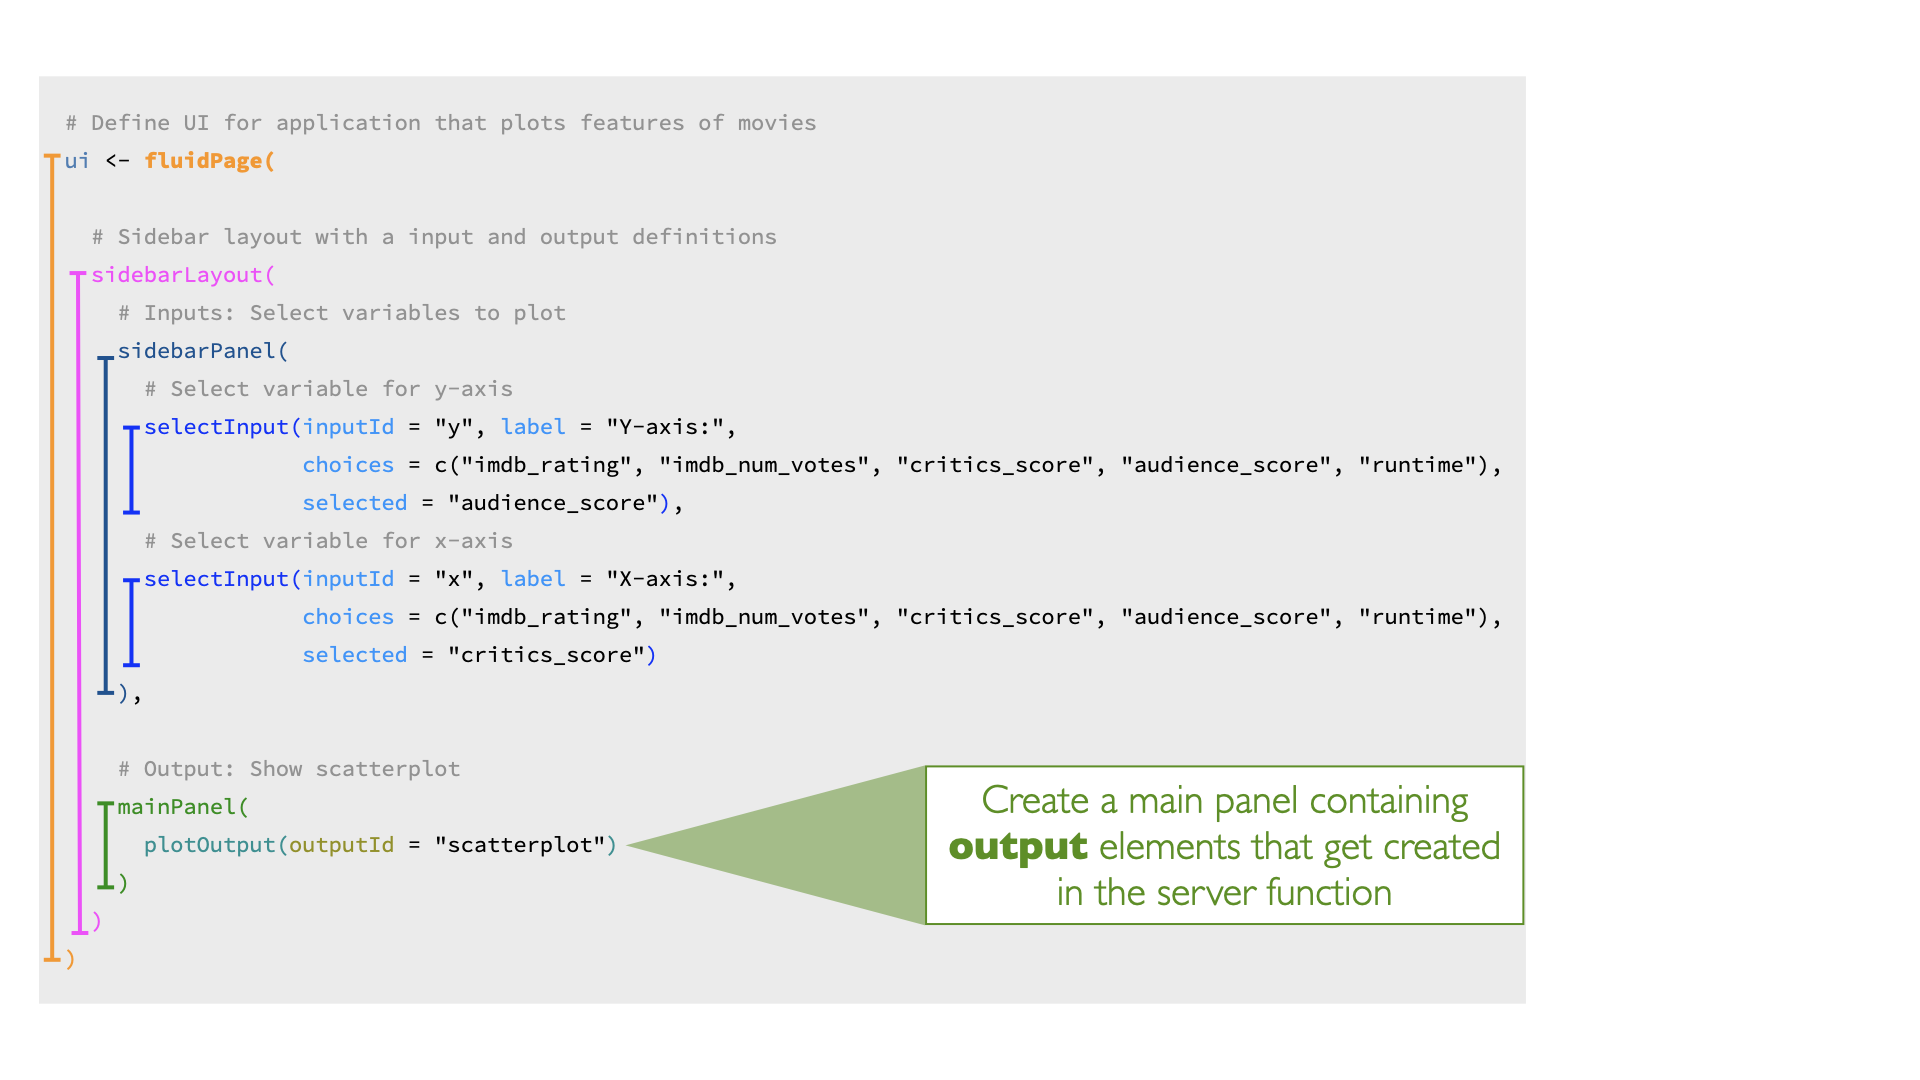
\includegraphics[width=1\textwidth,height=\textheight]{./images/main-panel.png}

}

\end{figure}

Currently the main panel contains only one component, a plot output.
We'll talk about how this plot is built later in the tutorial.

Next, let's practice building an app UI!

\hypertarget{practice-extend-the-ui}{%
\subsection{Practice: Extend the UI}\label{practice-extend-the-ui}}

We'll start with a simplified version of the app you saw in the previous
exercise. In this app a \texttt{selectInput()} widget is used to allow
the user to select which variables should be plotted on the \texttt{x}
and \texttt{y} axes of the scatterplot.

The \texttt{selectInput()} function has the following arguments:

\begin{itemize}
\tightlist
\item
  an \texttt{inputId} that is used to refer to the input parameter when
  building the scatterplot,
\item
  a list of \texttt{choices} to pick from (which must match variable
  names in the data frame),
\item
  and a \texttt{selected} choice for when the app first launches.
\end{itemize}

\hypertarget{your-turn-1}{%
\subsubsection{Your turn}\label{your-turn-1}}

Modify the Shiny app code in \texttt{app.R} / shown below:

\begin{itemize}
\tightlist
\item
  In the \texttt{ui}:

  \begin{itemize}
  \tightlist
  \item
    Add a new \texttt{selectInput} widget to color the points by a
    choice of the following variables: \texttt{"title\_type"},
    \texttt{"genre"}, \texttt{"mpaa\_rating"},
    \texttt{"critics\_rating"}, \texttt{"audience\_rating"}.
  \item
    Make the default selection \texttt{"mpaa\_rating"}.
  \item
    Use \texttt{"z"} as the \texttt{inputId}.
  \item
    \texttt{label} can be whatever you like.
  \end{itemize}
\item
  In the \texttt{server}:

  \begin{itemize}
  \tightlist
  \item
    Set the color argument in \texttt{ggplot()} aesthetic mappings to
    \texttt{input\$z}.
  \end{itemize}
\end{itemize}

\emph{Complete this exercise by opening up the RStudio Project titled
\textbf{1-2a Extend the UI} within your RStudio Cloud Workspace}

\href{https://rstudio.cloud/spaces/81721/join?access_code=I4VJaNsKfTqR3Td9hLP7E1nz8\%2FtMg6Xbw9Bgqumv}{
Go to RStudio Cloud Workspace}

\begin{Shaded}
\begin{Highlighting}[]
\CommentTok{\# Load packages {-}{-}{-}{-}{-}{-}{-}{-}{-}{-}{-}{-}{-}{-}{-}{-}{-}{-}{-}{-}{-}{-}{-}{-}{-}{-}{-}{-}{-}{-}{-}{-}{-}{-}{-}{-}{-}{-}{-}{-}{-}{-}{-}{-}{-}{-}{-}{-}{-}{-}{-}{-}{-}{-}{-}{-}{-}{-}{-}{-}{-}{-}{-}{-}}

\FunctionTok{library}\NormalTok{(shiny)}
\FunctionTok{library}\NormalTok{(ggplot2)}

\CommentTok{\# Load data {-}{-}{-}{-}{-}{-}{-}{-}{-}{-}{-}{-}{-}{-}{-}{-}{-}{-}{-}{-}{-}{-}{-}{-}{-}{-}{-}{-}{-}{-}{-}{-}{-}{-}{-}{-}{-}{-}{-}{-}{-}{-}{-}{-}{-}{-}{-}{-}{-}{-}{-}{-}{-}{-}{-}{-}{-}{-}{-}{-}{-}{-}{-}{-}{-}{-}{-}{-}}

\FunctionTok{load}\NormalTok{(}\StringTok{"movies.RData"}\NormalTok{)}

\CommentTok{\# Define UI {-}{-}{-}{-}{-}{-}{-}{-}{-}{-}{-}{-}{-}{-}{-}{-}{-}{-}{-}{-}{-}{-}{-}{-}{-}{-}{-}{-}{-}{-}{-}{-}{-}{-}{-}{-}{-}{-}{-}{-}{-}{-}{-}{-}{-}{-}{-}{-}{-}{-}{-}{-}{-}{-}{-}{-}{-}{-}{-}{-}{-}{-}{-}{-}{-}{-}{-}{-}}

\NormalTok{ui }\OtherTok{\textless{}{-}} \FunctionTok{fluidPage}\NormalTok{(}
  
  \FunctionTok{sidebarLayout}\NormalTok{(}
    
    \CommentTok{\# Inputs: Select variables to plot}
    \FunctionTok{sidebarPanel}\NormalTok{(}
      
      \CommentTok{\# Select variable for y{-}axis}
      \FunctionTok{selectInput}\NormalTok{(}\AttributeTok{inputId =} \StringTok{"y"}\NormalTok{, }
                  \AttributeTok{label =} \StringTok{"Y{-}axis:"}\NormalTok{,}
                  \AttributeTok{choices =} \FunctionTok{c}\NormalTok{(}\StringTok{"imdb\_rating"}\NormalTok{, }\StringTok{"imdb\_num\_votes"}\NormalTok{, }\StringTok{"critics\_score"}\NormalTok{, }\StringTok{"audience\_score"}\NormalTok{, }\StringTok{"runtime"}\NormalTok{), }
                  \AttributeTok{selected =} \StringTok{"audience\_score"}\NormalTok{),}
      
      \CommentTok{\# Select variable for x{-}axis}
      \FunctionTok{selectInput}\NormalTok{(}\AttributeTok{inputId =} \StringTok{"x"}\NormalTok{, }
                  \AttributeTok{label =} \StringTok{"X{-}axis:"}\NormalTok{,}
                  \AttributeTok{choices =} \FunctionTok{c}\NormalTok{(}\StringTok{"imdb\_rating"}\NormalTok{, }\StringTok{"imdb\_num\_votes"}\NormalTok{, }\StringTok{"critics\_score"}\NormalTok{, }\StringTok{"audience\_score"}\NormalTok{, }\StringTok{"runtime"}\NormalTok{), }
                  \AttributeTok{selected =} \StringTok{"critics\_score"}\NormalTok{),}
      
      \CommentTok{\# Select variable for color}
      \FunctionTok{selectInput}\NormalTok{(}\AttributeTok{inputId =} \StringTok{"\_\_\_"}\NormalTok{, }
                  \AttributeTok{label =} \StringTok{"\_\_\_\_"}\NormalTok{,}
                  \AttributeTok{choices =} \FunctionTok{c}\NormalTok{(\_\_\_),}
                  \AttributeTok{selected =} \StringTok{"\_\_\_"}\NormalTok{)}
      
\NormalTok{    ),}
    
    \CommentTok{\# Output: Show scatterplot}
    \FunctionTok{mainPanel}\NormalTok{(}
      \FunctionTok{plotOutput}\NormalTok{(}\AttributeTok{outputId =} \StringTok{"scatterplot"}\NormalTok{)}
\NormalTok{    )}
\NormalTok{  )}
\NormalTok{)}

\CommentTok{\# Define server {-}{-}{-}{-}{-}{-}{-}{-}{-}{-}{-}{-}{-}{-}{-}{-}{-}{-}{-}{-}{-}{-}{-}{-}{-}{-}{-}{-}{-}{-}{-}{-}{-}{-}{-}{-}{-}{-}{-}{-}{-}{-}{-}{-}{-}{-}{-}{-}{-}{-}{-}{-}{-}{-}{-}{-}{-}{-}{-}{-}{-}{-}{-}{-}}

\NormalTok{server }\OtherTok{\textless{}{-}} \ControlFlowTok{function}\NormalTok{(input, output, session) \{}
  
\NormalTok{  output}\SpecialCharTok{$}\NormalTok{scatterplot }\OtherTok{\textless{}{-}} \FunctionTok{renderPlot}\NormalTok{(\{}
    \FunctionTok{ggplot}\NormalTok{(}\AttributeTok{data =}\NormalTok{ movies, }\FunctionTok{aes\_string}\NormalTok{(}\AttributeTok{x =}\NormalTok{ input}\SpecialCharTok{$}\NormalTok{x, }\AttributeTok{y =}\NormalTok{ input}\SpecialCharTok{$}\NormalTok{y,}
                                     \AttributeTok{color =}\NormalTok{ \_\_\_)) }\SpecialCharTok{+}
      \FunctionTok{geom\_point}\NormalTok{()}
\NormalTok{  \})}
  
\NormalTok{  \}}

\CommentTok{\# Create a Shiny app object {-}{-}{-}{-}{-}{-}{-}{-}{-}{-}{-}{-}{-}{-}{-}{-}{-}{-}{-}{-}{-}{-}{-}{-}{-}{-}{-}{-}{-}{-}{-}{-}{-}{-}{-}{-}{-}{-}{-}{-}{-}{-}{-}{-}{-}{-}{-}{-}{-}{-}{-}{-}}

\FunctionTok{shinyApp}\NormalTok{(}\AttributeTok{ui =}\NormalTok{ ui, }\AttributeTok{server =}\NormalTok{ server)}
\end{Highlighting}
\end{Shaded}

Show solution

See the following code chunk for the solution to the exercise above.

\begin{Shaded}
\begin{Highlighting}[]
\CommentTok{\# Load packages {-}{-}{-}{-}{-}{-}{-}{-}{-}{-}{-}{-}{-}{-}{-}{-}{-}{-}{-}{-}{-}{-}{-}{-}{-}{-}{-}{-}{-}{-}{-}{-}{-}{-}{-}{-}{-}{-}{-}{-}{-}{-}{-}{-}{-}{-}{-}{-}{-}{-}{-}{-}{-}{-}{-}{-}{-}{-}{-}{-}{-}{-}{-}{-}}

\FunctionTok{library}\NormalTok{(shiny)}
\FunctionTok{library}\NormalTok{(ggplot2)}

\CommentTok{\# Load data {-}{-}{-}{-}{-}{-}{-}{-}{-}{-}{-}{-}{-}{-}{-}{-}{-}{-}{-}{-}{-}{-}{-}{-}{-}{-}{-}{-}{-}{-}{-}{-}{-}{-}{-}{-}{-}{-}{-}{-}{-}{-}{-}{-}{-}{-}{-}{-}{-}{-}{-}{-}{-}{-}{-}{-}{-}{-}{-}{-}{-}{-}{-}{-}{-}{-}{-}{-}}

\FunctionTok{load}\NormalTok{(}\StringTok{"movies.RData"}\NormalTok{)}

\CommentTok{\# Define UI {-}{-}{-}{-}{-}{-}{-}{-}{-}{-}{-}{-}{-}{-}{-}{-}{-}{-}{-}{-}{-}{-}{-}{-}{-}{-}{-}{-}{-}{-}{-}{-}{-}{-}{-}{-}{-}{-}{-}{-}{-}{-}{-}{-}{-}{-}{-}{-}{-}{-}{-}{-}{-}{-}{-}{-}{-}{-}{-}{-}{-}{-}{-}{-}{-}{-}{-}{-}}

\NormalTok{ui }\OtherTok{\textless{}{-}} \FunctionTok{fluidPage}\NormalTok{(}
  
  \FunctionTok{sidebarLayout}\NormalTok{(}
    
    \CommentTok{\# Inputs: Select variables to plot}
    \FunctionTok{sidebarPanel}\NormalTok{(}
      
      \CommentTok{\# Select variable for y{-}axis}
      \FunctionTok{selectInput}\NormalTok{(}\AttributeTok{inputId =} \StringTok{"y"}\NormalTok{, }
                  \AttributeTok{label =} \StringTok{"Y{-}axis:"}\NormalTok{,}
                  \AttributeTok{choices =} \FunctionTok{c}\NormalTok{(}\StringTok{"imdb\_rating"}\NormalTok{, }\StringTok{"imdb\_num\_votes"}\NormalTok{, }\StringTok{"critics\_score"}\NormalTok{, }\StringTok{"audience\_score"}\NormalTok{, }\StringTok{"runtime"}\NormalTok{), }
                  \AttributeTok{selected =} \StringTok{"audience\_score"}\NormalTok{),}
      
      \CommentTok{\# Select variable for x{-}axis}
      \FunctionTok{selectInput}\NormalTok{(}\AttributeTok{inputId =} \StringTok{"x"}\NormalTok{, }
                  \AttributeTok{label =} \StringTok{"X{-}axis:"}\NormalTok{,}
                  \AttributeTok{choices =} \FunctionTok{c}\NormalTok{(}\StringTok{"imdb\_rating"}\NormalTok{, }\StringTok{"imdb\_num\_votes"}\NormalTok{, }\StringTok{"critics\_score"}\NormalTok{, }\StringTok{"audience\_score"}\NormalTok{, }\StringTok{"runtime"}\NormalTok{), }
                  \AttributeTok{selected =} \StringTok{"critics\_score"}\NormalTok{),}
      
      \CommentTok{\# Select variable for color}
      \FunctionTok{selectInput}\NormalTok{(}\AttributeTok{inputId =} \StringTok{"z"}\NormalTok{, }
                  \AttributeTok{label =} \StringTok{"Color by:"}\NormalTok{,}
                  \AttributeTok{choices =} \FunctionTok{c}\NormalTok{(}\StringTok{"title\_type"}\NormalTok{, }\StringTok{"genre"}\NormalTok{, }\StringTok{"mpaa\_rating"}\NormalTok{, }\StringTok{"critics\_rating"}\NormalTok{, }\StringTok{"audience\_rating"}\NormalTok{),}
                  \AttributeTok{selected =} \StringTok{"mpaa\_rating"}\NormalTok{)}
      
\NormalTok{    ),}
    
    \CommentTok{\# Output: Show scatterplot}
    \FunctionTok{mainPanel}\NormalTok{(}
      \FunctionTok{plotOutput}\NormalTok{(}\AttributeTok{outputId =} \StringTok{"scatterplot"}\NormalTok{)}
\NormalTok{    )}
\NormalTok{  )}
\NormalTok{)}

\CommentTok{\# Define server {-}{-}{-}{-}{-}{-}{-}{-}{-}{-}{-}{-}{-}{-}{-}{-}{-}{-}{-}{-}{-}{-}{-}{-}{-}{-}{-}{-}{-}{-}{-}{-}{-}{-}{-}{-}{-}{-}{-}{-}{-}{-}{-}{-}{-}{-}{-}{-}{-}{-}{-}{-}{-}{-}{-}{-}{-}{-}{-}{-}{-}{-}{-}{-}}

\NormalTok{server }\OtherTok{\textless{}{-}} \ControlFlowTok{function}\NormalTok{(input, output, session) \{}
  
\NormalTok{  output}\SpecialCharTok{$}\NormalTok{scatterplot }\OtherTok{\textless{}{-}} \FunctionTok{renderPlot}\NormalTok{(\{}
    \FunctionTok{ggplot}\NormalTok{(}\AttributeTok{data =}\NormalTok{ movies, }\FunctionTok{aes\_string}\NormalTok{(}\AttributeTok{x =}\NormalTok{ input}\SpecialCharTok{$}\NormalTok{x, }\AttributeTok{y =}\NormalTok{ input}\SpecialCharTok{$}\NormalTok{y,}
                                     \AttributeTok{color =}\NormalTok{ input}\SpecialCharTok{$}\NormalTok{z)) }\SpecialCharTok{+}
      \FunctionTok{geom\_point}\NormalTok{()}
\NormalTok{  \})}
  
\NormalTok{  \}}

\CommentTok{\# Create a Shiny app object {-}{-}{-}{-}{-}{-}{-}{-}{-}{-}{-}{-}{-}{-}{-}{-}{-}{-}{-}{-}{-}{-}{-}{-}{-}{-}{-}{-}{-}{-}{-}{-}{-}{-}{-}{-}{-}{-}{-}{-}{-}{-}{-}{-}{-}{-}{-}{-}{-}{-}{-}{-}}

\FunctionTok{shinyApp}\NormalTok{(}\AttributeTok{ui =}\NormalTok{ ui, }\AttributeTok{server =}\NormalTok{ server)}
\end{Highlighting}
\end{Shaded}

\hypertarget{practice-extend-the-ui-further}{%
\subsection{Practice: Extend the UI
further}\label{practice-extend-the-ui-further}}

The potential variables the user can select for the \texttt{x} and
\texttt{y} axes and \texttt{color} currently appear in the UI of the app
the same way that they are spelled in the data frame header. However we
might want to label them in a way that is more human readable. We can
achieve this using named vectors for the \texttt{choices} argument, in
the format of \texttt{"Human\ readable\ label"\ =\ "variable\_name"}.

\hypertarget{your-turn-2}{%
\subsubsection{Your turn}\label{your-turn-2}}

\begin{itemize}
\tightlist
\item
  Fill in the blanks in the code below with human readable labels for
  \texttt{x} and \texttt{y} inputs.
\item
  Re-create the \texttt{selectInput} widget for color, \texttt{z}, with
  options \texttt{"title\_type"}, \texttt{"genre"},
  \texttt{"mpaa\_rating"}, \texttt{"critics\_rating"}, and
  \texttt{"audience\_rating"}, default selection \texttt{"mpaa\_rating"}
  just like in the previous exercise, but this time use human readable
  labels as well.
\end{itemize}

\emph{Complete this exercise by opening up the RStudio Project titled
\textbf{1-2b Extend the UI further} within your RStudio Cloud Workspace}

\href{https://rstudio.cloud/spaces/81721/join?access_code=I4VJaNsKfTqR3Td9hLP7E1nz8\%2FtMg6Xbw9Bgqumv}{
Go to RStudio Cloud Workspace}

\begin{Shaded}
\begin{Highlighting}[]
\CommentTok{\# Load packages {-}{-}{-}{-}{-}{-}{-}{-}{-}{-}{-}{-}{-}{-}{-}{-}{-}{-}{-}{-}{-}{-}{-}{-}{-}{-}{-}{-}{-}{-}{-}{-}{-}{-}{-}{-}{-}{-}{-}{-}{-}{-}{-}{-}{-}{-}{-}{-}{-}{-}{-}{-}{-}{-}{-}{-}{-}{-}{-}{-}{-}{-}{-}{-}}

\FunctionTok{library}\NormalTok{(shiny)}
\FunctionTok{library}\NormalTok{(ggplot2)}

\CommentTok{\# Load data {-}{-}{-}{-}{-}{-}{-}{-}{-}{-}{-}{-}{-}{-}{-}{-}{-}{-}{-}{-}{-}{-}{-}{-}{-}{-}{-}{-}{-}{-}{-}{-}{-}{-}{-}{-}{-}{-}{-}{-}{-}{-}{-}{-}{-}{-}{-}{-}{-}{-}{-}{-}{-}{-}{-}{-}{-}{-}{-}{-}{-}{-}{-}{-}{-}{-}{-}{-}}

\FunctionTok{load}\NormalTok{(}\StringTok{"movies.RData"}\NormalTok{)}

\CommentTok{\# Define UI {-}{-}{-}{-}{-}{-}{-}{-}{-}{-}{-}{-}{-}{-}{-}{-}{-}{-}{-}{-}{-}{-}{-}{-}{-}{-}{-}{-}{-}{-}{-}{-}{-}{-}{-}{-}{-}{-}{-}{-}{-}{-}{-}{-}{-}{-}{-}{-}{-}{-}{-}{-}{-}{-}{-}{-}{-}{-}{-}{-}{-}{-}{-}{-}{-}{-}{-}{-}}

\NormalTok{ui }\OtherTok{\textless{}{-}} \FunctionTok{fluidPage}\NormalTok{(}
  
  \FunctionTok{sidebarLayout}\NormalTok{(}
    
    \CommentTok{\# Inputs: Select variables to plot}
    \FunctionTok{sidebarPanel}\NormalTok{(}
      
      \CommentTok{\# Select variable for y{-}axis}
      \FunctionTok{selectInput}\NormalTok{(}\AttributeTok{inputId =} \StringTok{"y"}\NormalTok{, }
                  \AttributeTok{label =} \StringTok{"Y{-}axis:"}\NormalTok{,}
                  \AttributeTok{choices =} \FunctionTok{c}\NormalTok{(}\AttributeTok{\_\_\_ =} \StringTok{"imdb\_rating"}\NormalTok{, }
                              \AttributeTok{\_\_\_ =} \StringTok{"imdb\_num\_votes"}\NormalTok{, }
                              \AttributeTok{\_\_\_ =} \StringTok{"critics\_score"}\NormalTok{, }
                              \AttributeTok{\_\_\_ =} \StringTok{"audience\_score"}\NormalTok{, }
                              \AttributeTok{\_\_\_ =} \StringTok{"runtime"}\NormalTok{), }
                  \AttributeTok{selected =} \StringTok{"audience\_score"}\NormalTok{),}
      
      \CommentTok{\# Select variable for x{-}axis}
      \FunctionTok{selectInput}\NormalTok{(}\AttributeTok{inputId =} \StringTok{"x"}\NormalTok{, }
                  \AttributeTok{label =} \StringTok{"X{-}axis:"}\NormalTok{,}
                  \AttributeTok{choices =} \FunctionTok{c}\NormalTok{(}\AttributeTok{\_\_\_ =} \StringTok{"imdb\_rating"}\NormalTok{, }
                              \AttributeTok{\_\_\_ =} \StringTok{"imdb\_num\_votes"}\NormalTok{, }
                              \AttributeTok{\_\_\_ =} \StringTok{"critics\_score"}\NormalTok{, }
                              \AttributeTok{\_\_\_ =} \StringTok{"audience\_score"}\NormalTok{, }
                              \AttributeTok{\_\_\_ =} \StringTok{"runtime"}\NormalTok{), }
                  \AttributeTok{selected =} \StringTok{"critics\_score"}\NormalTok{),}
      
      \CommentTok{\# Select variable for color}
      \FunctionTok{selectInput}\NormalTok{(}\AttributeTok{inputId =} \StringTok{"z"}\NormalTok{, }
                  \AttributeTok{label =} \StringTok{"Color:"}\NormalTok{,}
                  \AttributeTok{choices =}\NormalTok{ \_\_\_, }
                  \AttributeTok{selected =}\NormalTok{ \_\_\_)}
      
\NormalTok{    ),}
    
    \CommentTok{\# Output: Show scatterplot}
    \FunctionTok{mainPanel}\NormalTok{(}
      \FunctionTok{plotOutput}\NormalTok{(}\AttributeTok{outputId =} \StringTok{"scatterplot"}\NormalTok{)}
\NormalTok{    )}
\NormalTok{  )}
\NormalTok{)}

\CommentTok{\# Define server {-}{-}{-}{-}{-}{-}{-}{-}{-}{-}{-}{-}{-}{-}{-}{-}{-}{-}{-}{-}{-}{-}{-}{-}{-}{-}{-}{-}{-}{-}{-}{-}{-}{-}{-}{-}{-}{-}{-}{-}{-}{-}{-}{-}{-}{-}{-}{-}{-}{-}{-}{-}{-}{-}{-}{-}{-}{-}{-}{-}{-}{-}{-}{-}}

\NormalTok{server }\OtherTok{\textless{}{-}} \ControlFlowTok{function}\NormalTok{(input, output, session) \{}
  
\NormalTok{  output}\SpecialCharTok{$}\NormalTok{scatterplot }\OtherTok{\textless{}{-}} \FunctionTok{renderPlot}\NormalTok{(\{}
    \FunctionTok{ggplot}\NormalTok{(}\AttributeTok{data =}\NormalTok{ movies, }\FunctionTok{aes\_string}\NormalTok{(}\AttributeTok{x =}\NormalTok{ input}\SpecialCharTok{$}\NormalTok{x, }\AttributeTok{y =}\NormalTok{ input}\SpecialCharTok{$}\NormalTok{y,}
                                     \AttributeTok{color =}\NormalTok{ input}\SpecialCharTok{$}\NormalTok{z)) }\SpecialCharTok{+}
      \FunctionTok{geom\_point}\NormalTok{()}
\NormalTok{  \})}
  
\NormalTok{  \}}

\CommentTok{\# Create a Shiny app object {-}{-}{-}{-}{-}{-}{-}{-}{-}{-}{-}{-}{-}{-}{-}{-}{-}{-}{-}{-}{-}{-}{-}{-}{-}{-}{-}{-}{-}{-}{-}{-}{-}{-}{-}{-}{-}{-}{-}{-}{-}{-}{-}{-}{-}{-}{-}{-}{-}{-}{-}{-}}

\FunctionTok{shinyApp}\NormalTok{(}\AttributeTok{ui =}\NormalTok{ ui, }\AttributeTok{server =}\NormalTok{ server)}
\end{Highlighting}
\end{Shaded}

Show solution

See the following code chunk for the solution to the exercise above.

\begin{Shaded}
\begin{Highlighting}[]
\CommentTok{\# Load packages {-}{-}{-}{-}{-}{-}{-}{-}{-}{-}{-}{-}{-}{-}{-}{-}{-}{-}{-}{-}{-}{-}{-}{-}{-}{-}{-}{-}{-}{-}{-}{-}{-}{-}{-}{-}{-}{-}{-}{-}{-}{-}{-}{-}{-}{-}{-}{-}{-}{-}{-}{-}{-}{-}{-}{-}{-}{-}{-}{-}{-}{-}{-}{-}}

\FunctionTok{library}\NormalTok{(shiny)}
\FunctionTok{library}\NormalTok{(ggplot2)}

\CommentTok{\# Load data {-}{-}{-}{-}{-}{-}{-}{-}{-}{-}{-}{-}{-}{-}{-}{-}{-}{-}{-}{-}{-}{-}{-}{-}{-}{-}{-}{-}{-}{-}{-}{-}{-}{-}{-}{-}{-}{-}{-}{-}{-}{-}{-}{-}{-}{-}{-}{-}{-}{-}{-}{-}{-}{-}{-}{-}{-}{-}{-}{-}{-}{-}{-}{-}{-}{-}{-}{-}}

\FunctionTok{load}\NormalTok{(}\StringTok{"movies.RData"}\NormalTok{)}

\CommentTok{\# Define UI {-}{-}{-}{-}{-}{-}{-}{-}{-}{-}{-}{-}{-}{-}{-}{-}{-}{-}{-}{-}{-}{-}{-}{-}{-}{-}{-}{-}{-}{-}{-}{-}{-}{-}{-}{-}{-}{-}{-}{-}{-}{-}{-}{-}{-}{-}{-}{-}{-}{-}{-}{-}{-}{-}{-}{-}{-}{-}{-}{-}{-}{-}{-}{-}{-}{-}{-}{-}}

\NormalTok{ui }\OtherTok{\textless{}{-}} \FunctionTok{fluidPage}\NormalTok{(}
  
  \FunctionTok{sidebarLayout}\NormalTok{(}
    
    \CommentTok{\# Inputs: Select variables to plot}
    \FunctionTok{sidebarPanel}\NormalTok{(}
      
      \CommentTok{\# Select variable for y{-}axis}
      \FunctionTok{selectInput}\NormalTok{(}\AttributeTok{inputId =} \StringTok{"y"}\NormalTok{, }
                  \AttributeTok{label =} \StringTok{"Y{-}axis:"}\NormalTok{,}
                  \AttributeTok{choices =} \FunctionTok{c}\NormalTok{(}\StringTok{"IMDB rating"}          \OtherTok{=} \StringTok{"imdb\_rating"}\NormalTok{, }
                              \StringTok{"IMDB number of votes"} \OtherTok{=} \StringTok{"imdb\_num\_votes"}\NormalTok{, }
                              \StringTok{"Critics score"}        \OtherTok{=} \StringTok{"critics\_score"}\NormalTok{, }
                              \StringTok{"Audience score"}       \OtherTok{=} \StringTok{"audience\_score"}\NormalTok{, }
                              \StringTok{"Runtime"}              \OtherTok{=} \StringTok{"runtime"}\NormalTok{), }
                  \AttributeTok{selected =} \StringTok{"audience\_score"}\NormalTok{),}
      
      \CommentTok{\# Select variable for x{-}axis}
      \FunctionTok{selectInput}\NormalTok{(}\AttributeTok{inputId =} \StringTok{"x"}\NormalTok{, }
                  \AttributeTok{label =} \StringTok{"X{-}axis:"}\NormalTok{,}
                  \AttributeTok{choices =} \FunctionTok{c}\NormalTok{(}
                    \StringTok{"IMDB rating"}          \OtherTok{=} \StringTok{"imdb\_rating"}\NormalTok{, }
                    \StringTok{"IMDB number of votes"} \OtherTok{=} \StringTok{"imdb\_num\_votes"}\NormalTok{, }
                    \StringTok{"Critics score"}        \OtherTok{=} \StringTok{"critics\_score"}\NormalTok{, }
                    \StringTok{"Audience score"}       \OtherTok{=} \StringTok{"audience\_score"}\NormalTok{, }
                    \StringTok{"Runtime"}              \OtherTok{=} \StringTok{"runtime"}\NormalTok{), }
                  \AttributeTok{selected =} \StringTok{"critics\_score"}\NormalTok{),}
      
      \CommentTok{\# Select variable for color}
      \CommentTok{\# Select variable for color}
      \FunctionTok{selectInput}\NormalTok{(}\AttributeTok{inputId =} \StringTok{"z"}\NormalTok{, }
                  \AttributeTok{label =} \StringTok{"Color by:"}\NormalTok{,}
                  \AttributeTok{choices =} \FunctionTok{c}\NormalTok{(}
                    \StringTok{"Title type"} \OtherTok{=} \StringTok{"title\_type"}\NormalTok{, }
                    \StringTok{"Genre"} \OtherTok{=} \StringTok{"genre"}\NormalTok{, }
                    \StringTok{"MPAA rating"} \OtherTok{=} \StringTok{"mpaa\_rating"}\NormalTok{, }
                    \StringTok{"Critics rating"} \OtherTok{=} \StringTok{"critics\_rating"}\NormalTok{, }
                    \StringTok{"Audience rating"} \OtherTok{=} \StringTok{"audience\_rating"}\NormalTok{),}
                  \AttributeTok{selected =} \StringTok{"mpaa\_rating"}\NormalTok{)}
      
\NormalTok{    ),}
    
    \CommentTok{\# Output: Show scatterplot}
    \FunctionTok{mainPanel}\NormalTok{(}
      \FunctionTok{plotOutput}\NormalTok{(}\AttributeTok{outputId =} \StringTok{"scatterplot"}\NormalTok{)}
\NormalTok{    )}
\NormalTok{  )}
\NormalTok{)}

\CommentTok{\# Define server {-}{-}{-}{-}{-}{-}{-}{-}{-}{-}{-}{-}{-}{-}{-}{-}{-}{-}{-}{-}{-}{-}{-}{-}{-}{-}{-}{-}{-}{-}{-}{-}{-}{-}{-}{-}{-}{-}{-}{-}{-}{-}{-}{-}{-}{-}{-}{-}{-}{-}{-}{-}{-}{-}{-}{-}{-}{-}{-}{-}{-}{-}{-}{-}}

\NormalTok{server }\OtherTok{\textless{}{-}} \ControlFlowTok{function}\NormalTok{(input, output, session) \{}
  
\NormalTok{  output}\SpecialCharTok{$}\NormalTok{scatterplot }\OtherTok{\textless{}{-}} \FunctionTok{renderPlot}\NormalTok{(\{}
    \FunctionTok{ggplot}\NormalTok{(}\AttributeTok{data =}\NormalTok{ movies, }\FunctionTok{aes\_string}\NormalTok{(}\AttributeTok{x =}\NormalTok{ input}\SpecialCharTok{$}\NormalTok{x, }\AttributeTok{y =}\NormalTok{ input}\SpecialCharTok{$}\NormalTok{y,}
                                     \AttributeTok{color =}\NormalTok{ input}\SpecialCharTok{$}\NormalTok{z)) }\SpecialCharTok{+}
      \FunctionTok{geom\_point}\NormalTok{()}
\NormalTok{  \})}
  
\NormalTok{  \}}

\CommentTok{\# Create a Shiny app object {-}{-}{-}{-}{-}{-}{-}{-}{-}{-}{-}{-}{-}{-}{-}{-}{-}{-}{-}{-}{-}{-}{-}{-}{-}{-}{-}{-}{-}{-}{-}{-}{-}{-}{-}{-}{-}{-}{-}{-}{-}{-}{-}{-}{-}{-}{-}{-}{-}{-}{-}{-}}

\FunctionTok{shinyApp}\NormalTok{(}\AttributeTok{ui =}\NormalTok{ ui, }\AttributeTok{server =}\NormalTok{ server)}
\end{Highlighting}
\end{Shaded}

\hypertarget{server-function}{%
\section{Server function}\label{server-function}}

Now that you've had some practice with the UI, it's time to move on to
the server function.

Again, before we get into the details, let's remind ourselves of the
anatomy of a Shiny app. The basic task of the server function is to
define the relationship between inputs and outputs.

\hypertarget{here-again-is-the-app-that-we-are-working-with-in-this-module}{%
\subsection{Here again is the app that we are working with in this
module}\label{here-again-is-the-app-that-we-are-working-with-in-this-module}}

Earlier we saw how to build the UI of this app, and we also noted that
each input was tagged with an \texttt{inputId} that can be used to refer
to them in the server.

\begin{figure}

{\centering 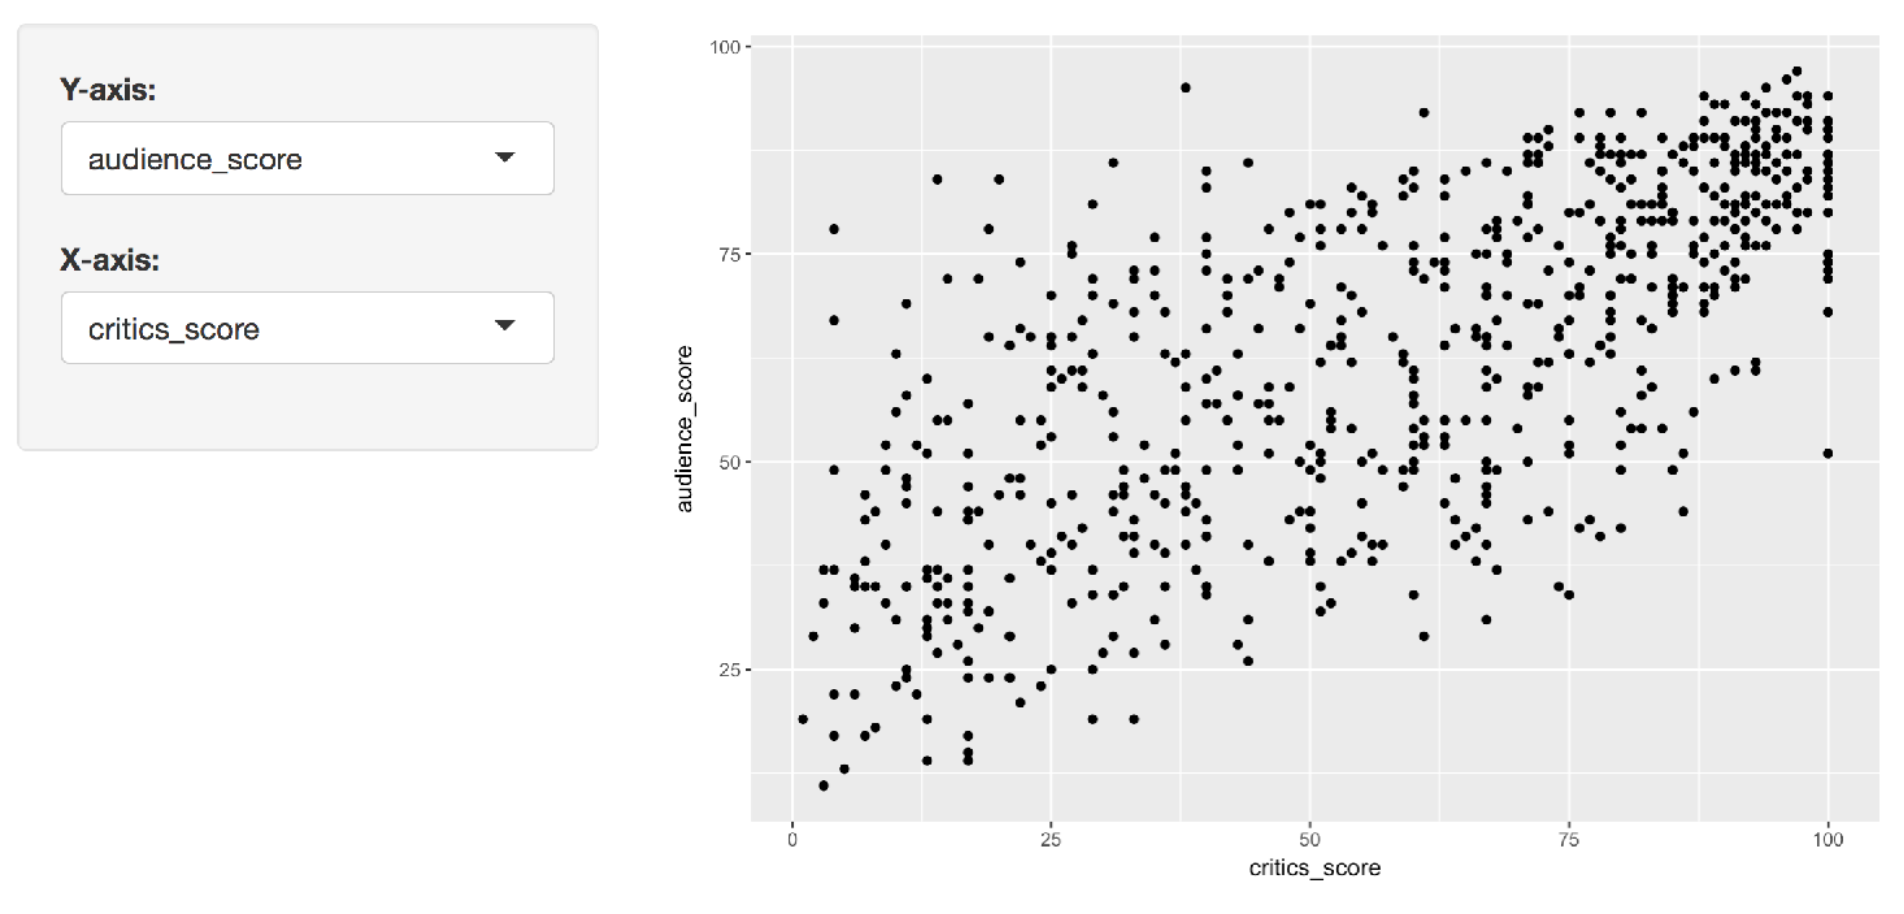
\includegraphics[width=1\textwidth,height=\textheight]{./images/app-selectinput-scatterplot.png}

}

\end{figure}

\hypertarget{this-is-the-server-function-code-for-this-app}{%
\subsection{This is the server function code for this
app}\label{this-is-the-server-function-code-for-this-app}}

Once again there is a lot going on here to parse at once, so in the
following sections we take a closer look at the function.

\begin{figure}

{\centering 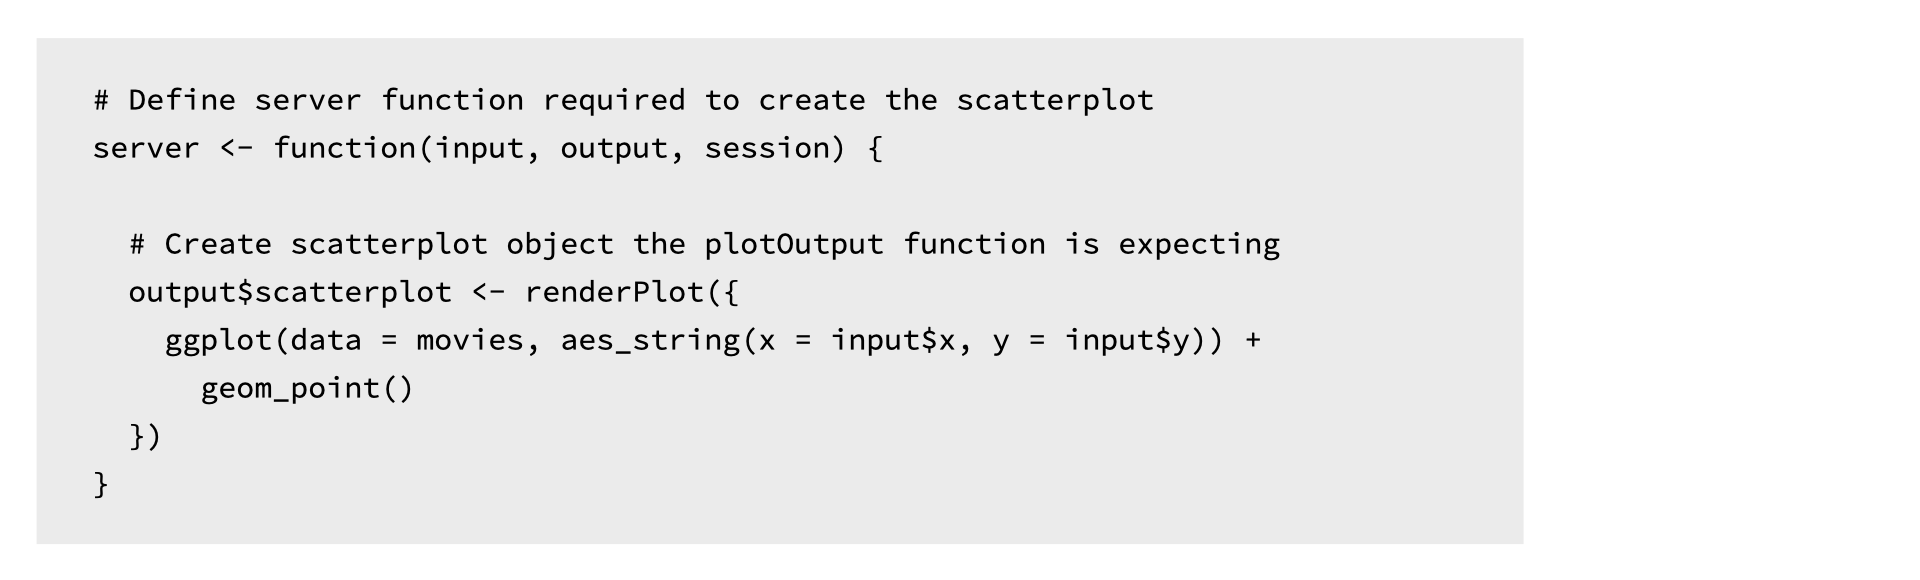
\includegraphics[width=1\textwidth,height=\textheight]{./images/server.png}

}

\end{figure}

\hypertarget{at-the-outermost-layer}{%
\subsection{At the outermost layer}\label{at-the-outermost-layer}}

\begin{figure}

{\centering 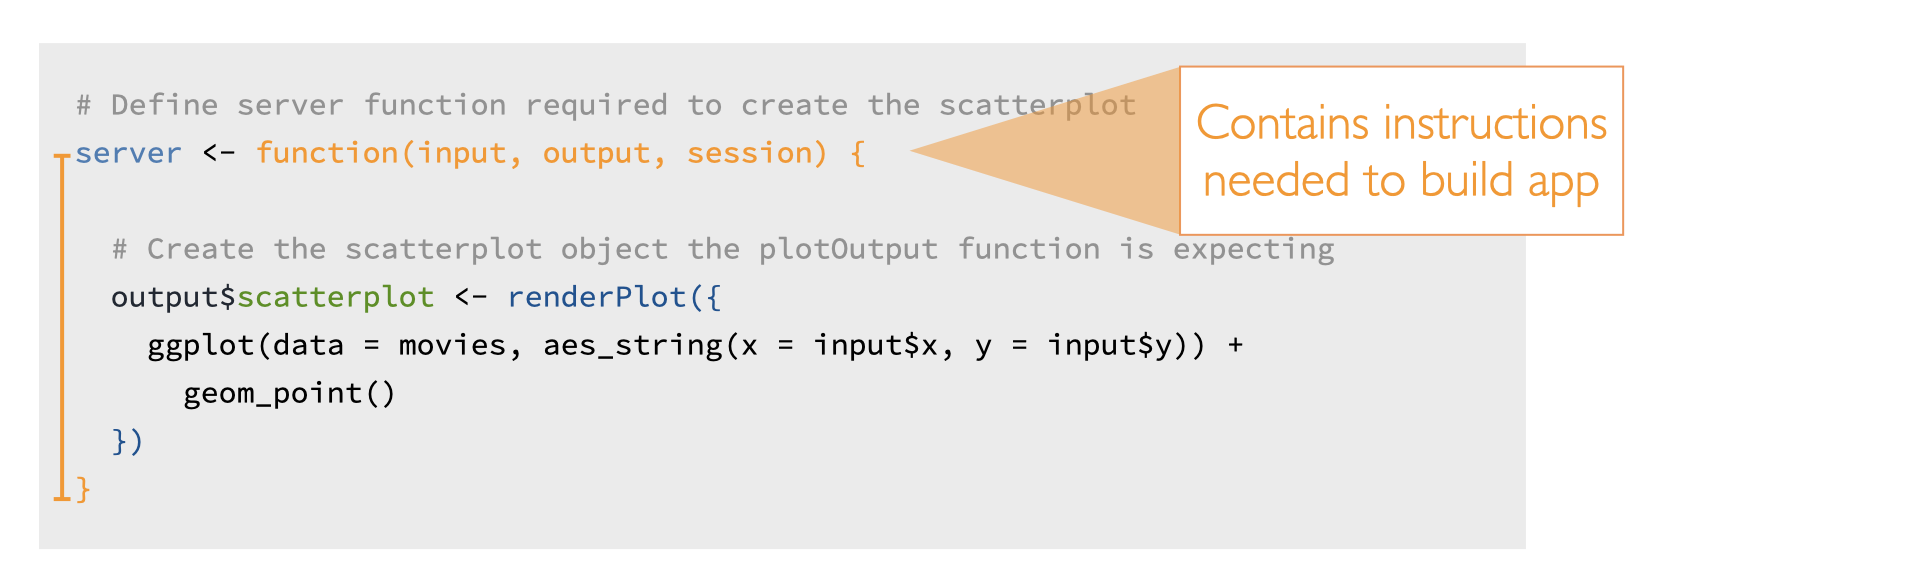
\includegraphics[width=1\textwidth,height=\textheight]{./images/server-outermost.png}

}

\end{figure}

We define our server function which takes two arguments: an
\texttt{input} and an \texttt{output}. Both of these are named lists.

The server function accesses inputs selected by the user to perform
computations and specifies how outputs laid out in the UI should be
updated.

The server function can take on one more argument, \texttt{session},
which is an environment that can be used to access information and
functionality relating to the session. However this concept is beyond
the scope of this tutorial, so for now we'll stick to server functions
that only have input and output arguments.

\hypertarget{output}{%
\subsection{\texorpdfstring{\texttt{output}}{output}}\label{output}}

Our simple app had only one output -- a plot. So our server function
contains the logic necessary to build this plot.

\begin{figure}

{\centering 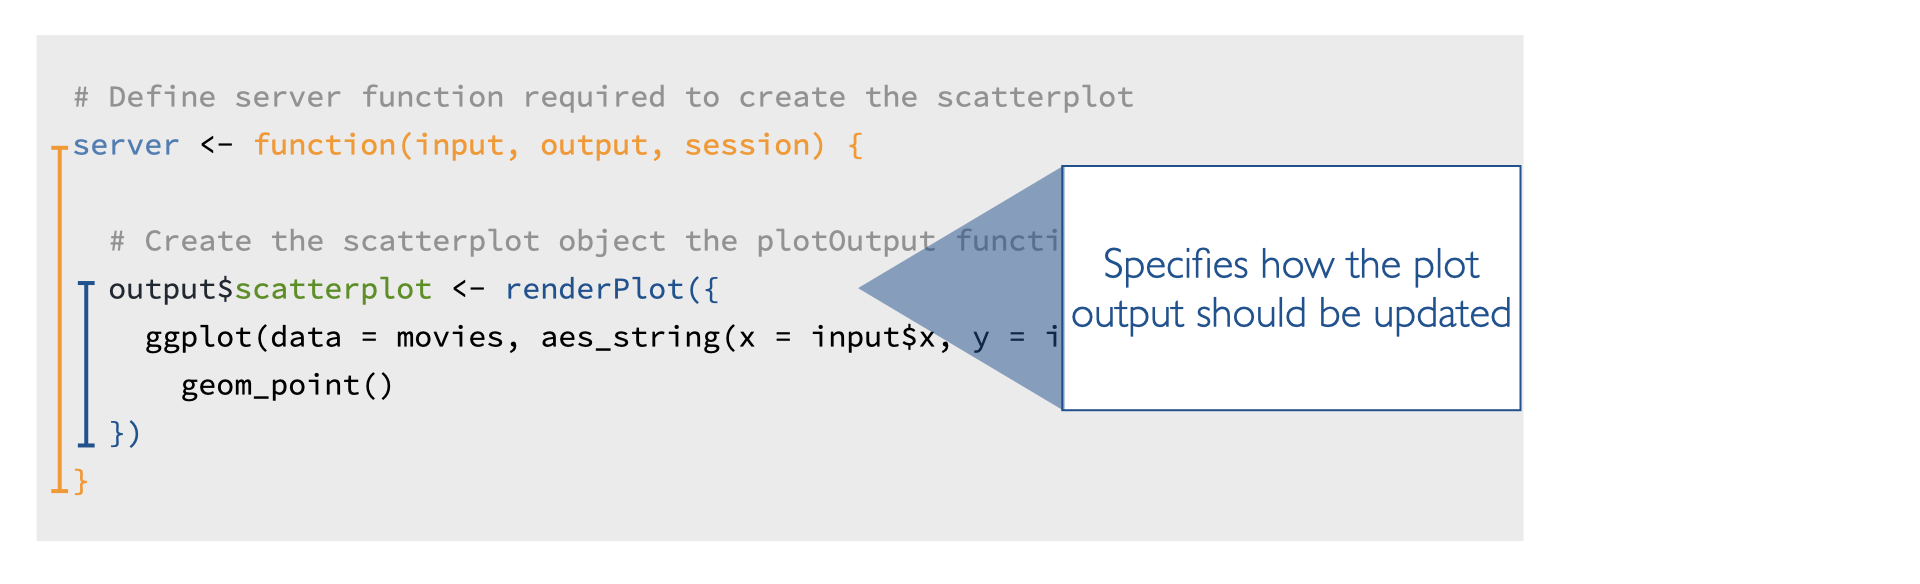
\includegraphics[width=1\textwidth,height=\textheight]{./images/output.png}

}

\end{figure}

The \texttt{renderPlot()} function specifies how the plot output should
be updated. Let's take a look at what is happening in the
\texttt{renderPlot()} function first.

\hypertarget{renderplot}{%
\subsection{\texorpdfstring{\texttt{renderPlot()}}{renderPlot()}}\label{renderplot}}

\begin{figure}

{\centering 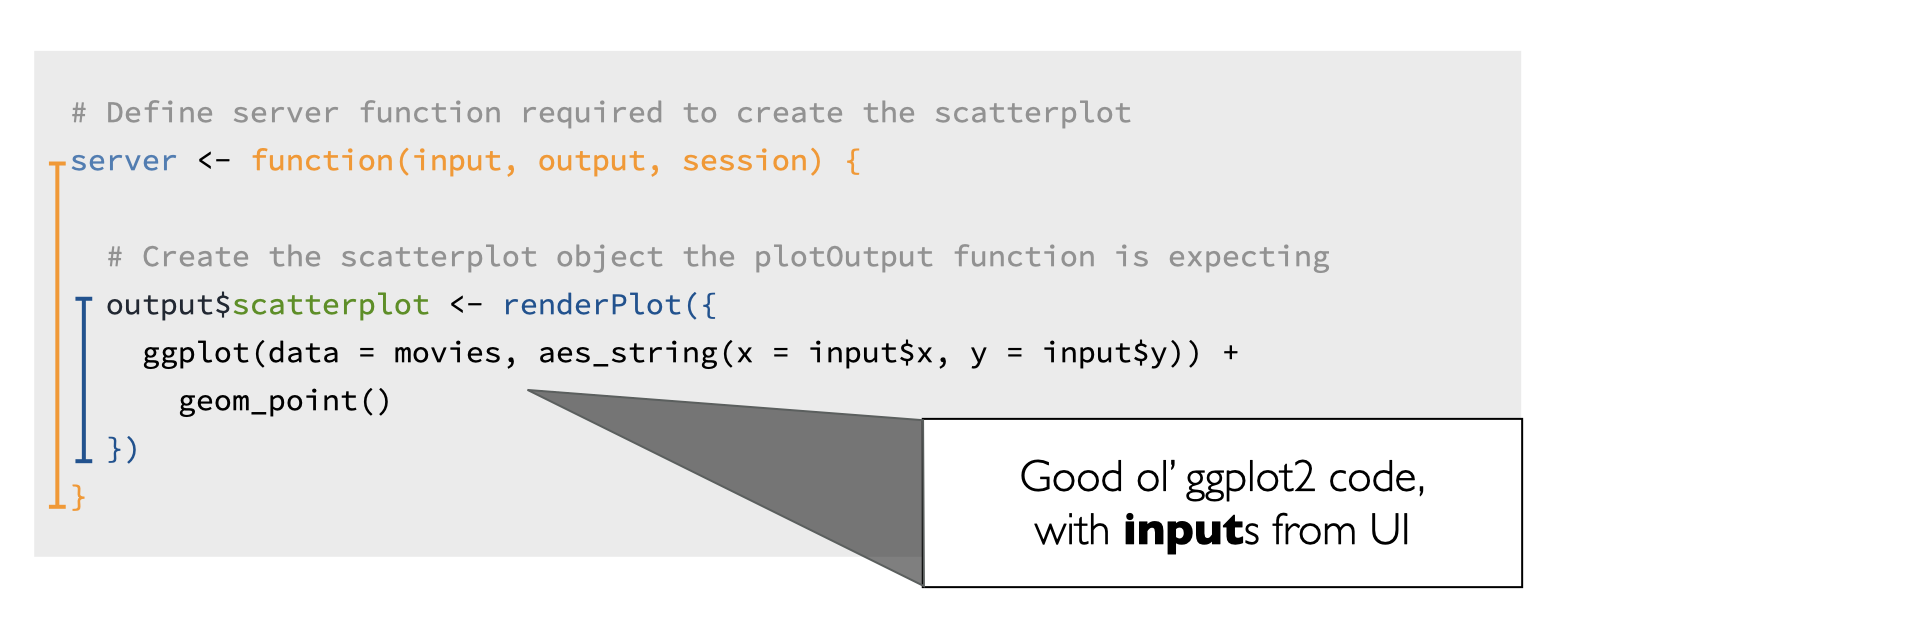
\includegraphics[width=1\textwidth,height=\textheight]{./images/renderplot.png}

}

\end{figure}

This is good ol' ggplot2 code! So even if you're new to shiny, if you've
previously used ggplot2 for plotting in R, this syntax should look
familiar to you.

One aspect of the syntax that might be new, however, is how the x and y
variables are defined. They come from the input list that is built in
the UI.

\hypertarget{inputs}{%
\subsection{Inputs}\label{inputs}}

Here is the relevant UI and server code.

\begin{figure}

{\centering 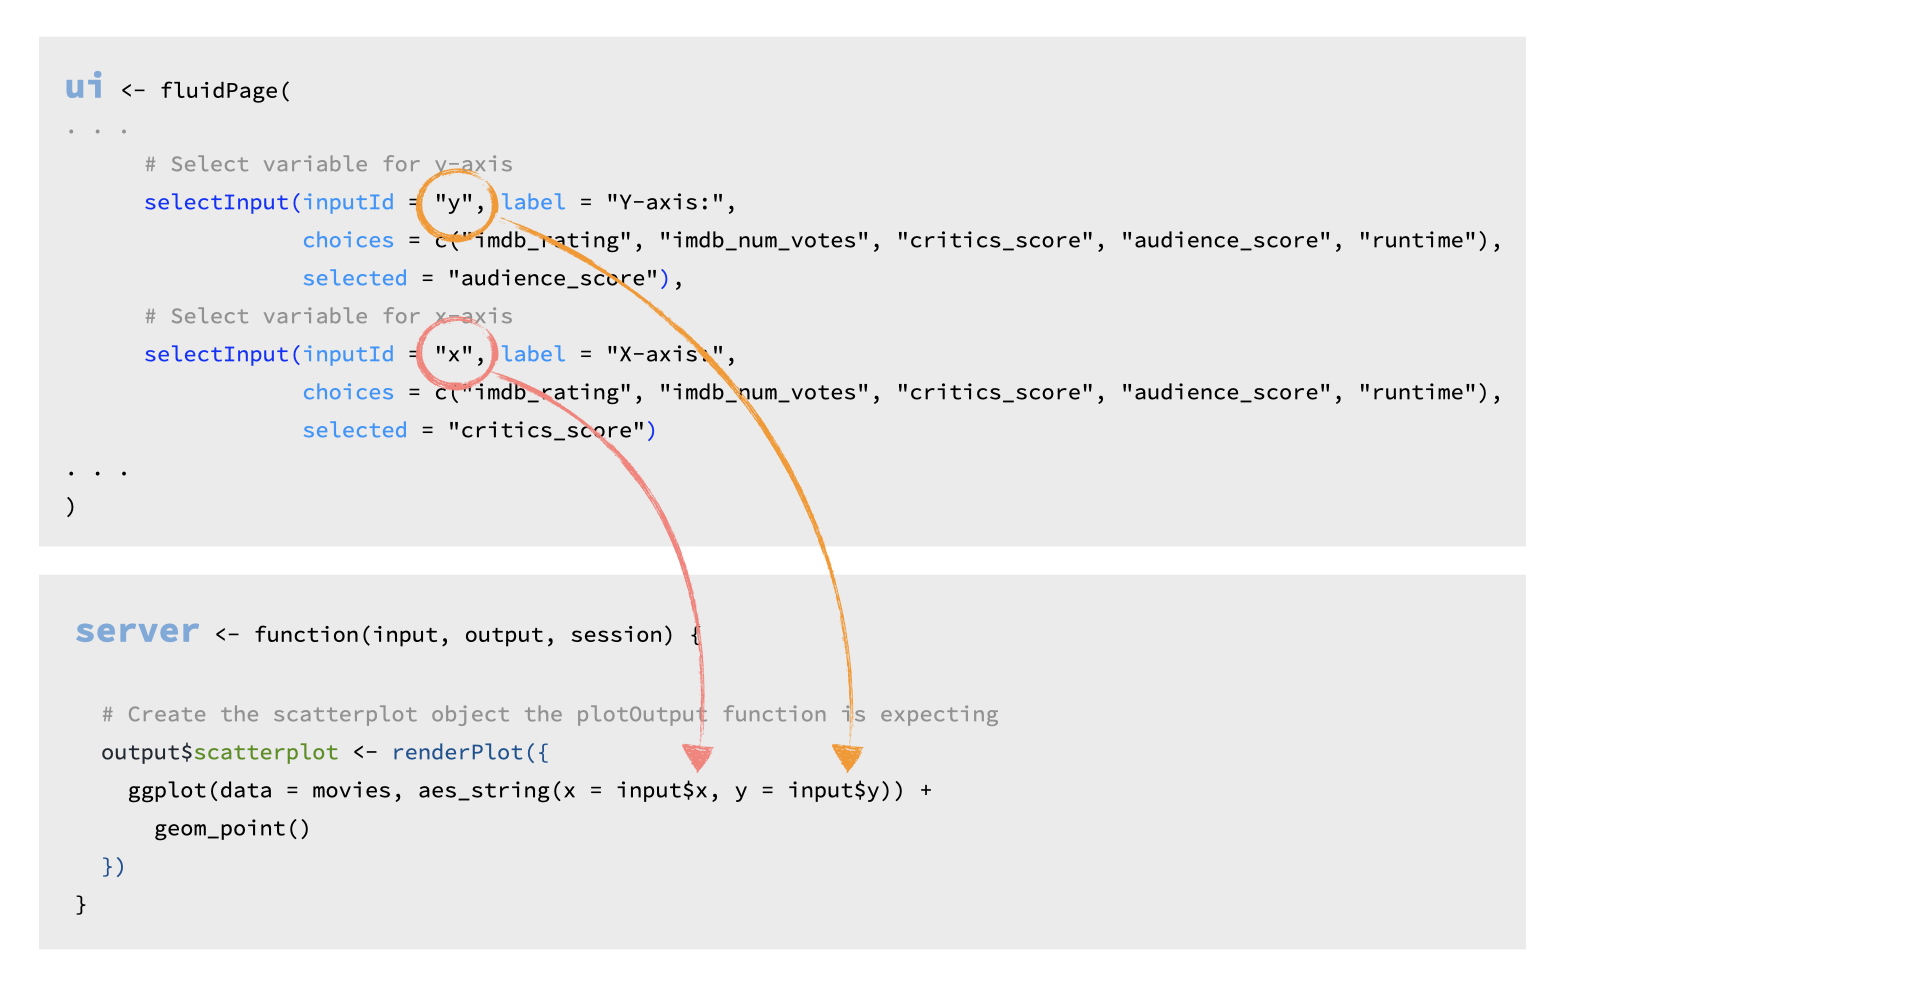
\includegraphics[width=1\textwidth,height=\textheight]{./images/inputs-x-y.png}

}

\end{figure}

Input x and y come from the \texttt{selectInput()} widgets, and map to
the \texttt{x} and \texttt{y} arguments of the plot aesthetics.

\hypertarget{rules-of-server-functions}{%
\subsection{Rules of server functions}\label{rules-of-server-functions}}

There are three rules of building server functions:

\begin{enumerate}
\def\labelenumi{\arabic{enumi}.}
\item
  Always save objects to display to the named output list,
  i.e.~something of the form \texttt{output\$xx}, where \texttt{xx} is
  the plot you want to display.
\item
  Always build objects to display with one of the \texttt{render*()}
  functions, like we built our plot with \texttt{renderPlot()}.
\item
  Use input values from the named input list, with \texttt{input\$xx}.
\end{enumerate}

\hypertarget{output-types}{%
\subsection{Output types}\label{output-types}}

Just like various inputs, Shiny also provides a wide selection of output
types each of which works with a render function.

\begin{figure}

{\centering 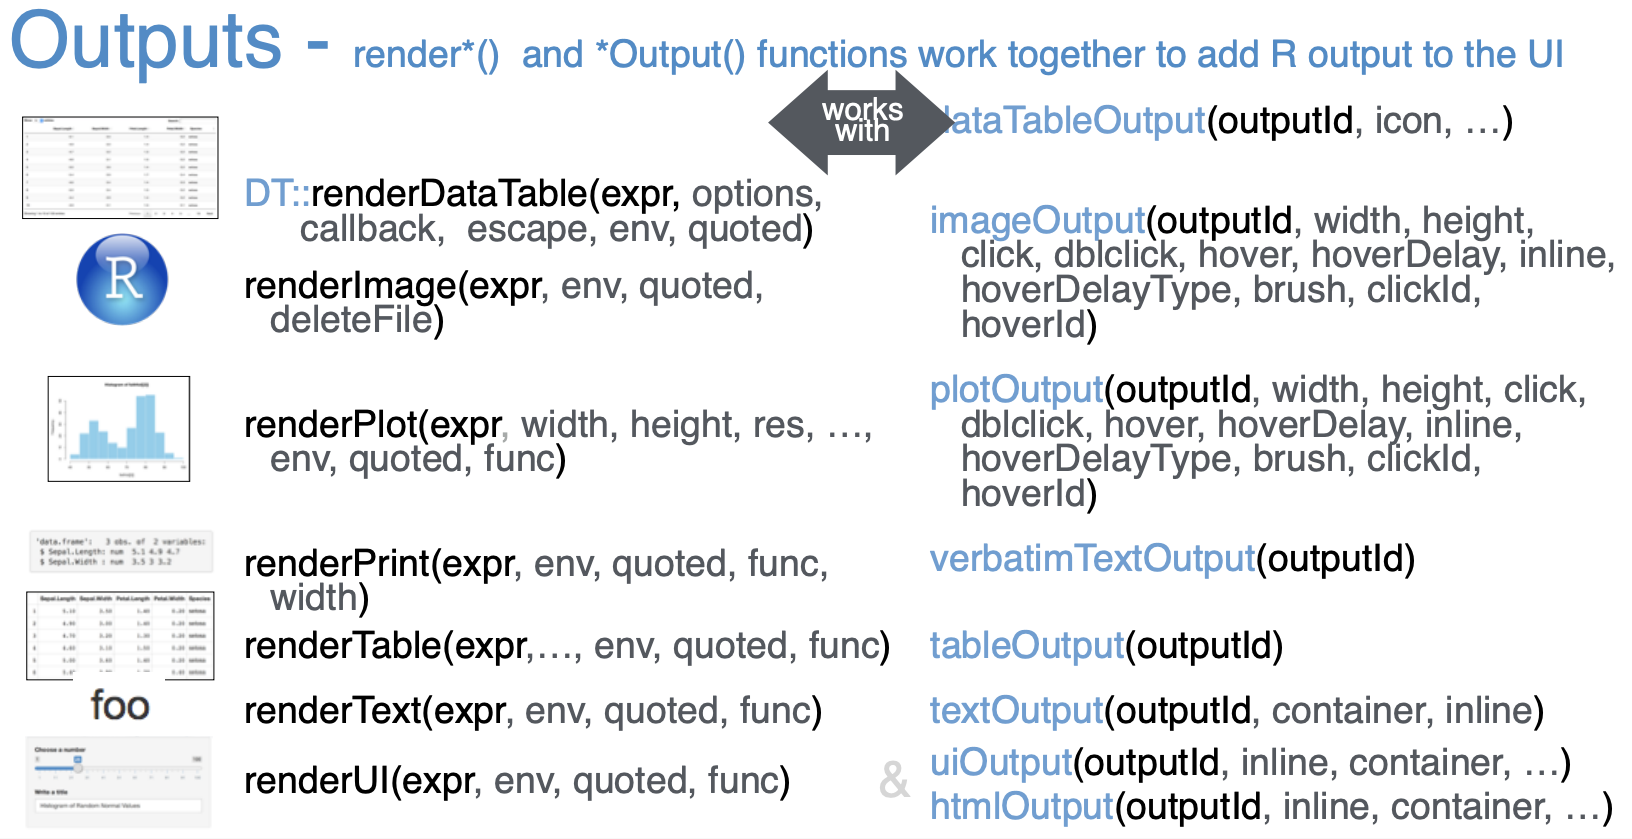
\includegraphics[width=0.8\textwidth,height=\textheight]{./images/cheatsheet-outputs.png}

}

\end{figure}

For example, in our app we used the \texttt{renderPlot()} function to
build our reactive plot (we'll get to what I mean by reactive in a
second) and laid out the plot with the \texttt{plotOutput()} function.

\begin{figure}

{\centering 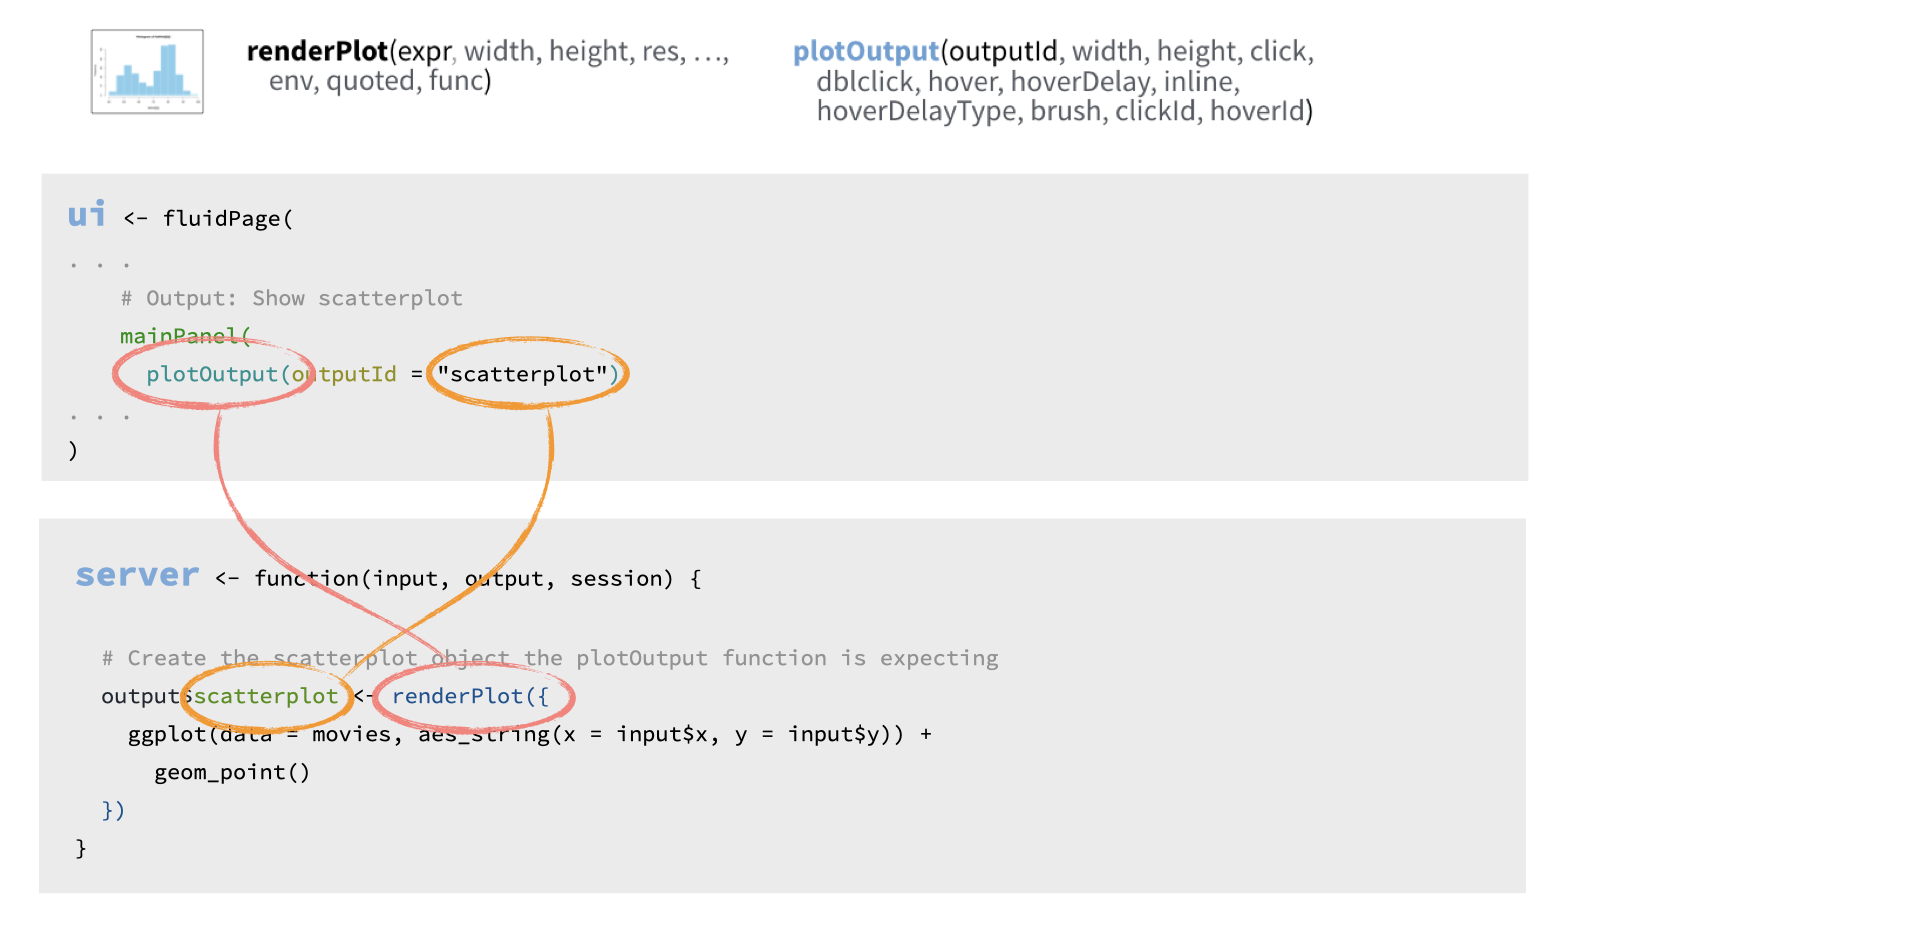
\includegraphics[width=1\textwidth,height=\textheight]{./images/render-output-pairs.png}

}

\end{figure}

Shiny knows to match these two together as they use the same
\texttt{outputID}, scatterplot.

In the following exercises you'll get a chance to work with other
render/output function pairs to add more elements to your app.

\hypertarget{practice-matching-inputs-and-outputs}{%
\subsection{Practice: Matching inputs and
outputs}\label{practice-matching-inputs-and-outputs}}

Here is a simple Shiny app. Try entering some text and observe how the
text is displayed back to you after a short pause.

\begin{center}\rule{0.5\linewidth}{0.5pt}\end{center}

\#\texttt{\{r,\ context\ =\ "server",\ eval\ =\ TRUE\}\ \#\ output\$user\_text\ \textless{}-\ renderText(\{\ input\$custom\_text\ \})\ \#}

\begin{center}\rule{0.5\linewidth}{0.5pt}\end{center}

The code for this app is given below, with a few pieces missing
(indicated with \texttt{\_\_\_}). Each of the blanks are numbered,
e.g.~(\texttt{{[}1{]}}, \texttt{{[}2{]}}, etc.)

\begin{Shaded}
\begin{Highlighting}[]
\FunctionTok{library}\NormalTok{(shiny)}

\NormalTok{ui }\OtherTok{\textless{}{-}} \FunctionTok{fluidPage}\NormalTok{(}

  \FunctionTok{textInput}\NormalTok{(}
    \AttributeTok{inputId =} \StringTok{"custom\_text"}\NormalTok{,}
    \AttributeTok{label =} \StringTok{"\_[1]\_"}
\NormalTok{  ),}

  \FunctionTok{strong}\NormalTok{(}\StringTok{"Text is shown below:"}\NormalTok{),}

\NormalTok{  \_[}\DecValTok{2}\NormalTok{]}\FunctionTok{\_}\NormalTok{(}\AttributeTok{outputId =} \StringTok{"\_[3]\_"}\NormalTok{)}

\NormalTok{)}

\NormalTok{server }\OtherTok{\textless{}{-}} \ControlFlowTok{function}\NormalTok{(input, output, session)\{}

\NormalTok{  output}\SpecialCharTok{$}\NormalTok{user\_text }\OtherTok{\textless{}{-}} \FunctionTok{renderText}\NormalTok{(\{ input}\SpecialCharTok{$}\NormalTok{\_[}\DecValTok{4}\NormalTok{]\_ \})}

\NormalTok{\}}

\FunctionTok{shinyApp}\NormalTok{(}\AttributeTok{ui =}\NormalTok{ ui, }\AttributeTok{server =}\NormalTok{ server)}
\end{Highlighting}
\end{Shaded}

\#\texttt{\{r\ mc-2\}\ \#question("Which\ of\ the\ following\ is\ false?",\ \#\ \ answer(\textquotesingle{}\textasciigrave{}{[}1{]}\textasciigrave{}\ should\ be\ \textasciigrave{}"Input\ some\ text\ here:"\textasciigrave{}\textquotesingle{},\ \#\ \ \ \ \ \ \ \ \ message\ =\ "Take\ a\ look\ at\ the\ app,\ what\ text\ is\ \#shown\ to\ the\ user\ above\ the\ text\ input\ area?"),\ \#\ \ answer(\textquotesingle{}\textasciigrave{}{[}2{]}\textasciigrave{}\ should\ be\ \textasciigrave{}textOutput\textasciigrave{}\textquotesingle{},\ \ \#\ \ \ \ \ \ \ \ \ message\ =\ "Check\ out\ the\ Shiny\ cheatsheet\ for\ pairs\ \#of\ input\ and\ output\ functions"),\ \#\ \ answer(\textquotesingle{}\textasciigrave{}{[}3{]}\textasciigrave{}\ should\ be\ \textasciigrave{}"custom\_text"\textasciigrave{}\textquotesingle{},\ correct\ =\ TRUE),\ \#\ \ answer(\textquotesingle{}\textasciigrave{}{[}4{]}\textasciigrave{}\ should\ be\ \textasciigrave{}"custom\_text"\textasciigrave{}\textquotesingle{},\ \#\ \ \ \ \ \ \ \ \ message\ =\ "What\ is\ the\ ID\ of\ the\ input\ that\ should\ \#be\ rendered?"),\ \#\ \ allow\_retry\ =\ TRUE\ \#)\ \#}

\hypertarget{reactivity}{%
\subsection{Reactivity}\label{reactivity}}

Let's also briefly discuss reactivity.

\begin{figure}

{\centering 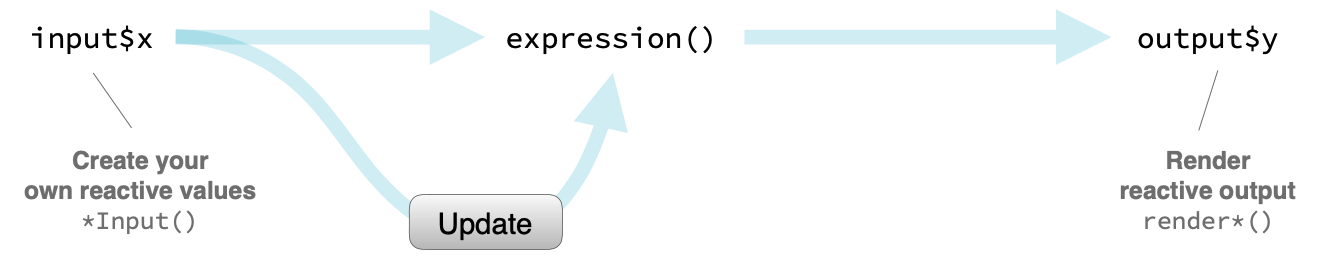
\includegraphics[width=0.8\textwidth,height=\textheight]{./images/reactivity.png}

}

\end{figure}

It's easy to build interactive applications with Shiny, but to get the
most out of it, you'll need to understand the reactive programming
scheme used by Shiny.

In a nutshell Shiny automatically updates outputs, such as plots, when
inputs that go into them change.

\hypertarget{putting-all-the-pieces-together}{%
\subsection{Putting all the pieces
together}\label{putting-all-the-pieces-together}}

Before we wrap up this section, I should also mention the last component
of each Shiny app, which is a call to the aptly named
\texttt{shinyApp()} function, which puts the UI and the server pieces
together to create a Shiny app object.

\begin{figure}

{\centering 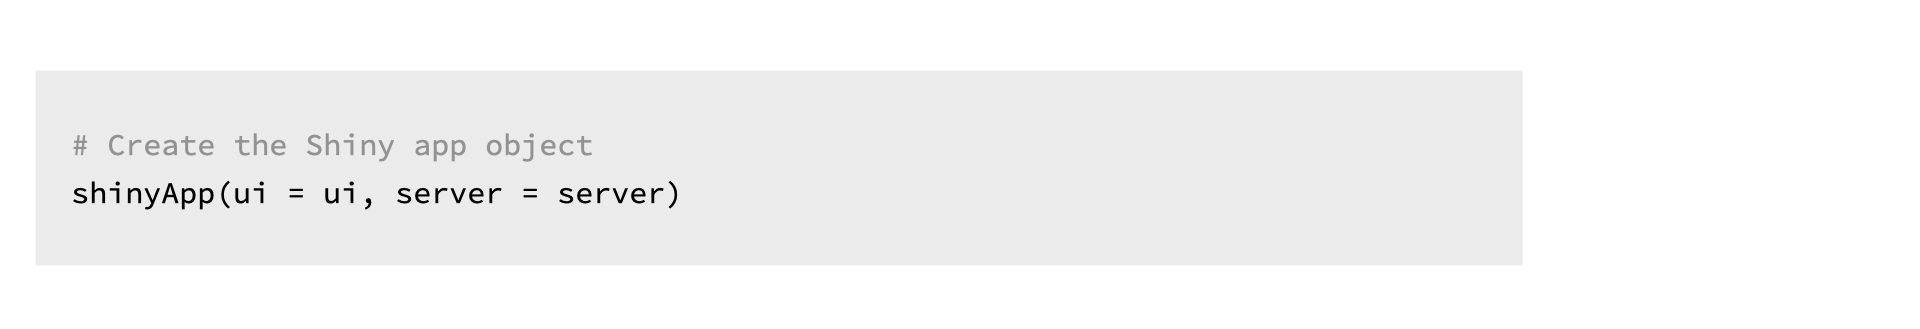
\includegraphics[width=0.8\textwidth,height=\textheight]{./images/shinyAppfunction.png}

}

\end{figure}

Time to put this all into practice!

\hypertarget{practice-rules-of-server-functions}{%
\subsection{Practice: Rules of server
functions}\label{practice-rules-of-server-functions}}

Which of the following is not true about server functions?

\#\texttt{\{r\ mc-3\}\ \#question("Which\ of\ the\ following\ is\ not\ true\ about\ server\ functions?",\ \#\ \ answer("Server\ functions\ should\ include\ a\ call\ to\ \#\textasciigrave{}runApp()\textasciigrave{}",\ \#\ \ \ \ correct\ =\ TRUE,\ \#\ \ \ \ message\ =\ "The\ \textasciigrave{}runApp()\textasciigrave{}\ function\ can\ be\ used\ in\ the\ Console\ to\ run\ a\ Shiny\ application,\ as\ an\ alternative\ to\ the\ Run\ App\ button\ in\ the\ RStudio\ IDE."\ \#\ \ ),\ \#\ \ answer("Objects\ to\ be\ displayed\ should\ be\ saved\ to\ \#\textasciigrave{}output\$\textasciigrave{}"),\ \#\ \ answer("Reactive\ objects\ should\ be\ built\ with\ \textasciigrave{}render*()\textasciigrave{}\ functions"),\ \#\ \ answer("Input\ values\ should\ be\ referred\ to\ with\ \textasciigrave{}input\$\textasciigrave{}"),\ \#\ \ allow\_retry\ =\ TRUE,\ \#\ \ random\_answer\_order\ =\ TRUE\ \#)\ \#}

\hypertarget{practice-fix-it-up}{%
\subsection{Practice: Fix it up}\label{practice-fix-it-up}}

Below is the code for the Shiny app we built earlier, however currently
the code is broken. Specifically there are errors in the definition of
the server function as well as in the \texttt{mainPanel} of the UI.

\hypertarget{your-turn-3}{%
\subsubsection{Your turn}\label{your-turn-3}}

\begin{itemize}
\tightlist
\item
  Review the app and identify errors in the code.

  \begin{itemize}
  \tightlist
  \item
    Hint: Refer back to the rules of server functions.
  \end{itemize}
\item
  Do the render functions match the output functions? If not, make the
  appropriate change and try running the app. Are there any remaining
  errors?
\item
  Are the inputs referred to using the correct syntax? If not, make the
  appropriate change and try running the app. Are there any remaining
  errors?
\item
  Are the outputs referred to using the correct names? If not, make the
  appropriate change and try running the app. Are there any remaining
  errors?
\end{itemize}

\emph{Navigate to the project called \textbf{1-3 Fix it up} after
clicking the button below}

\href{https://rstudio.cloud/spaces/81721/join?access_code=I4VJaNsKfTqR3Td9hLP7E1nz8\%2FtMg6Xbw9Bgqumv}{
Go to RStudio Cloud Workspace}

\begin{Shaded}
\begin{Highlighting}[]
\CommentTok{\# Load packages {-}{-}{-}{-}{-}{-}{-}{-}{-}{-}{-}{-}{-}{-}{-}{-}{-}{-}{-}{-}{-}{-}{-}{-}{-}{-}{-}{-}{-}{-}{-}{-}{-}{-}{-}{-}{-}{-}{-}{-}{-}{-}{-}{-}{-}{-}{-}{-}{-}{-}{-}{-}{-}{-}{-}{-}{-}{-}{-}{-}{-}{-}{-}{-}}

\FunctionTok{library}\NormalTok{(shiny)}
\FunctionTok{library}\NormalTok{(ggplot2)}

\CommentTok{\# Load data {-}{-}{-}{-}{-}{-}{-}{-}{-}{-}{-}{-}{-}{-}{-}{-}{-}{-}{-}{-}{-}{-}{-}{-}{-}{-}{-}{-}{-}{-}{-}{-}{-}{-}{-}{-}{-}{-}{-}{-}{-}{-}{-}{-}{-}{-}{-}{-}{-}{-}{-}{-}{-}{-}{-}{-}{-}{-}{-}{-}{-}{-}{-}{-}{-}{-}{-}{-}}

\FunctionTok{load}\NormalTok{(}\StringTok{"movies.RData"}\NormalTok{)}

\CommentTok{\# Define UI {-}{-}{-}{-}{-}{-}{-}{-}{-}{-}{-}{-}{-}{-}{-}{-}{-}{-}{-}{-}{-}{-}{-}{-}{-}{-}{-}{-}{-}{-}{-}{-}{-}{-}{-}{-}{-}{-}{-}{-}{-}{-}{-}{-}{-}{-}{-}{-}{-}{-}{-}{-}{-}{-}{-}{-}{-}{-}{-}{-}{-}{-}{-}{-}{-}{-}{-}{-}}

\NormalTok{ui }\OtherTok{\textless{}{-}} \FunctionTok{fluidPage}\NormalTok{(}
  \FunctionTok{sidebarLayout}\NormalTok{(}

    \CommentTok{\# Inputs: Select variables to plot}
    \FunctionTok{sidebarPanel}\NormalTok{(}

      \CommentTok{\# Select variable for y{-}axis}
      \FunctionTok{selectInput}\NormalTok{(}
        \AttributeTok{inputId =} \StringTok{"y"}\NormalTok{,}
        \AttributeTok{label =} \StringTok{"Y{-}axis:"}\NormalTok{,}
        \AttributeTok{choices =} \FunctionTok{c}\NormalTok{(}
          \StringTok{"IMDB rating"} \OtherTok{=} \StringTok{"imdb\_rating"}\NormalTok{,}
          \StringTok{"IMDB number of votes"} \OtherTok{=} \StringTok{"imdb\_num\_votes"}\NormalTok{,}
          \StringTok{"Critics score"} \OtherTok{=} \StringTok{"critics\_score"}\NormalTok{,}
          \StringTok{"Audience score"} \OtherTok{=} \StringTok{"audience\_score"}\NormalTok{,}
          \StringTok{"Runtime"} \OtherTok{=} \StringTok{"runtime"}
\NormalTok{        ),}
        \AttributeTok{selected =} \StringTok{"audience\_score"}
\NormalTok{      ),}

      \CommentTok{\# Select variable for x{-}axis}
      \FunctionTok{selectInput}\NormalTok{(}
        \AttributeTok{inputId =} \StringTok{"x"}\NormalTok{,}
        \AttributeTok{label =} \StringTok{"X{-}axis:"}\NormalTok{,}
        \AttributeTok{choices =} \FunctionTok{c}\NormalTok{(}
          \StringTok{"IMDB rating"} \OtherTok{=} \StringTok{"imdb\_rating"}\NormalTok{,}
          \StringTok{"IMDB number of votes"} \OtherTok{=} \StringTok{"imdb\_num\_votes"}\NormalTok{,}
          \StringTok{"Critics score"} \OtherTok{=} \StringTok{"critics\_score"}\NormalTok{,}
          \StringTok{"Audience score"} \OtherTok{=} \StringTok{"audience\_score"}\NormalTok{,}
          \StringTok{"Runtime"} \OtherTok{=} \StringTok{"runtime"}
\NormalTok{        ),}
        \AttributeTok{selected =} \StringTok{"critics\_score"}
\NormalTok{      ),}

      \CommentTok{\# Select variable for color}
      \FunctionTok{selectInput}\NormalTok{(}
        \AttributeTok{inputId =} \StringTok{"z"}\NormalTok{,}
        \AttributeTok{label =} \StringTok{"Color by:"}\NormalTok{,}
        \AttributeTok{choices =} \FunctionTok{c}\NormalTok{(}
          \StringTok{"Title type"} \OtherTok{=} \StringTok{"title\_type"}\NormalTok{,}
          \StringTok{"Genre"} \OtherTok{=} \StringTok{"genre"}\NormalTok{,}
          \StringTok{"MPAA rating"} \OtherTok{=} \StringTok{"mpaa\_rating"}\NormalTok{,}
          \StringTok{"Critics rating"} \OtherTok{=} \StringTok{"critics\_rating"}\NormalTok{,}
          \StringTok{"Audience rating"} \OtherTok{=} \StringTok{"audience\_rating"}
\NormalTok{        ),}
        \AttributeTok{selected =} \StringTok{"mpaa\_rating"}
\NormalTok{      )}
\NormalTok{    ),}

    \CommentTok{\# Output: Show scatterplot}
    \FunctionTok{mainPanel}\NormalTok{(}
      \FunctionTok{plotOutput}\NormalTok{(}\AttributeTok{outputId =} \StringTok{"scatterPlot"}\NormalTok{)}
\NormalTok{    )}
\NormalTok{  )}
\NormalTok{)}

\CommentTok{\# Define server {-}{-}{-}{-}{-}{-}{-}{-}{-}{-}{-}{-}{-}{-}{-}{-}{-}{-}{-}{-}{-}{-}{-}{-}{-}{-}{-}{-}{-}{-}{-}{-}{-}{-}{-}{-}{-}{-}{-}{-}{-}{-}{-}{-}{-}{-}{-}{-}{-}{-}{-}{-}{-}{-}{-}{-}{-}{-}{-}{-}{-}{-}{-}{-}}

\NormalTok{server }\OtherTok{\textless{}{-}} \ControlFlowTok{function}\NormalTok{(input, output, session) \{}
\NormalTok{  output}\SpecialCharTok{$}\NormalTok{scatterplot }\OtherTok{\textless{}{-}} \FunctionTok{renderTable}\NormalTok{(\{}

    \FunctionTok{ggplot}\NormalTok{(}\AttributeTok{data =}\NormalTok{ movies, }\FunctionTok{aes\_string}\NormalTok{(}\AttributeTok{x =}\NormalTok{ x, }\AttributeTok{y =}\NormalTok{ y, }\AttributeTok{color =}\NormalTok{ z)) }\SpecialCharTok{+}
      \FunctionTok{geom\_point}\NormalTok{()}

\NormalTok{  \})}

\NormalTok{\}}

\CommentTok{\# Create a Shiny app object {-}{-}{-}{-}{-}{-}{-}{-}{-}{-}{-}{-}{-}{-}{-}{-}{-}{-}{-}{-}{-}{-}{-}{-}{-}{-}{-}{-}{-}{-}{-}{-}{-}{-}{-}{-}{-}{-}{-}{-}{-}{-}{-}{-}{-}{-}{-}{-}{-}{-}{-}{-}}

\FunctionTok{shinyApp}\NormalTok{(}\AttributeTok{ui =}\NormalTok{ ui, }\AttributeTok{server =}\NormalTok{ server)}
\end{Highlighting}
\end{Shaded}

\hypertarget{recap}{%
\section{Recap}\label{recap}}

Let's quickly recap what we have learned in this chapter.

\hypertarget{section-4}{%
\subsection{}\label{section-4}}

Every Shiny app has a webpage that the user visits, and behind this
webpage there is a computer that serves this webpage by running R.

\begin{figure}

{\centering 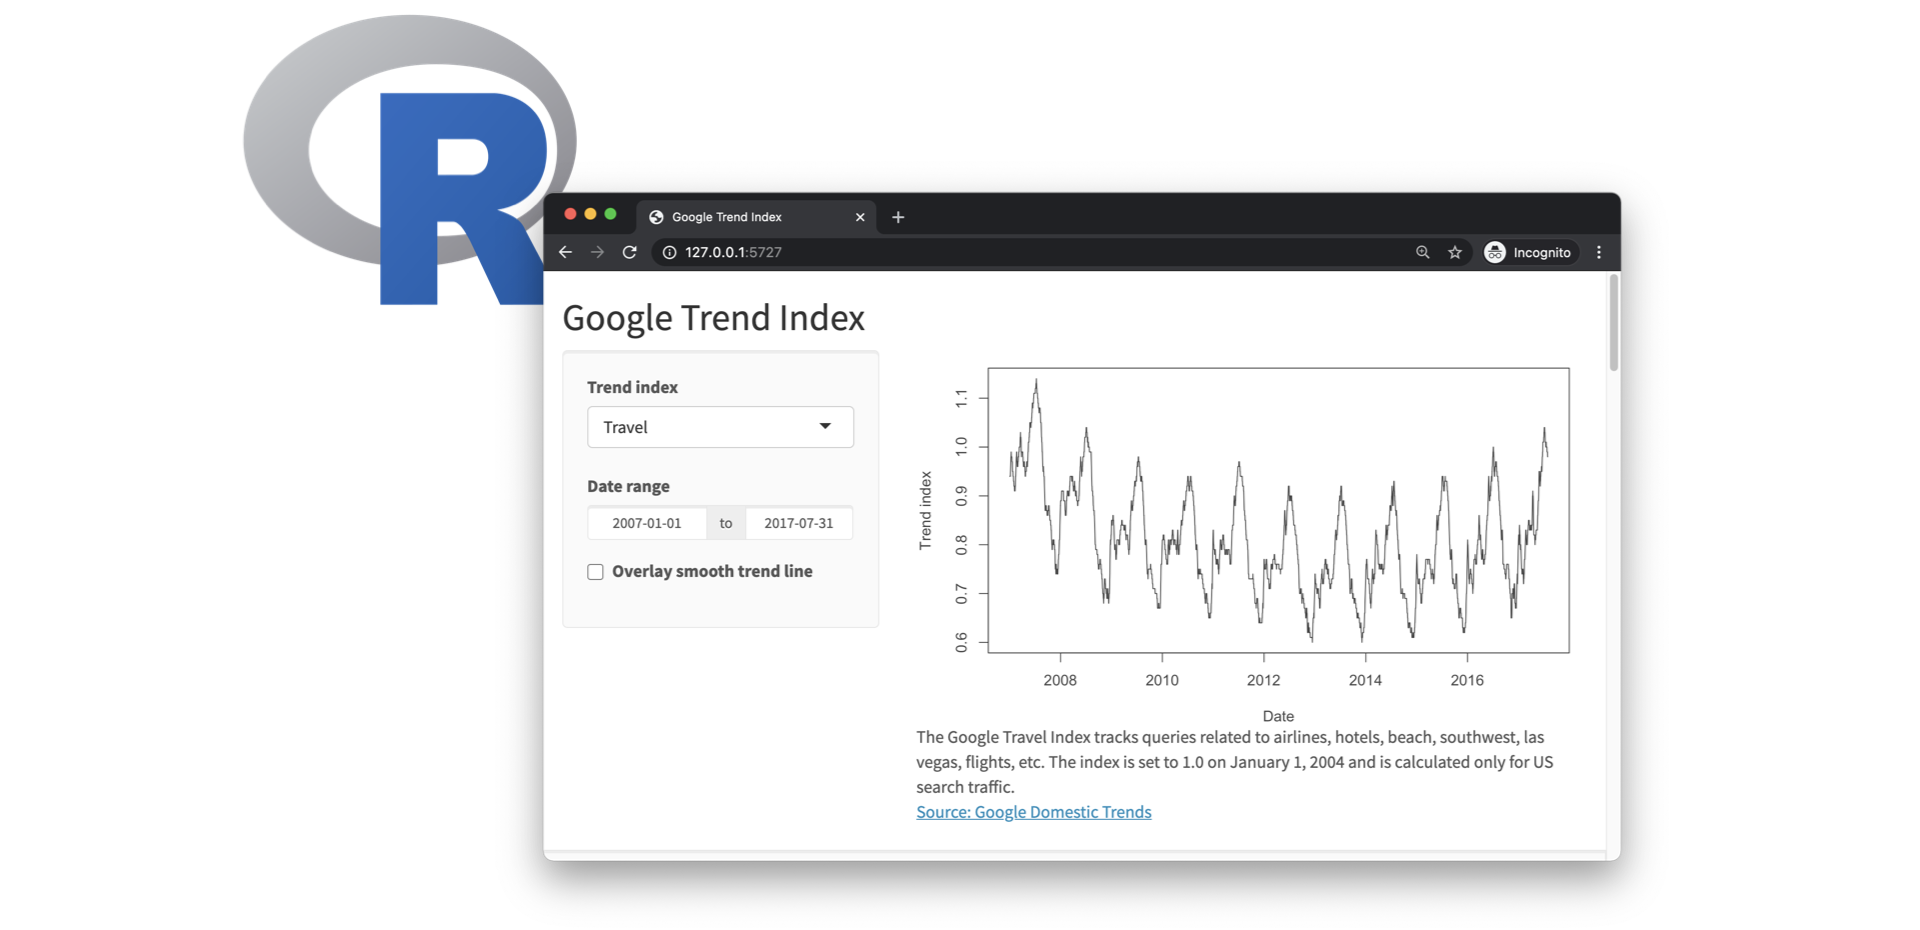
\includegraphics[width=0.8\textwidth,height=\textheight]{./images/recap-1.png}

}

\end{figure}

\hypertarget{section-5}{%
\subsection{}\label{section-5}}

When running your app locally, the computer serving your app is your
computer.

\begin{figure}

{\centering 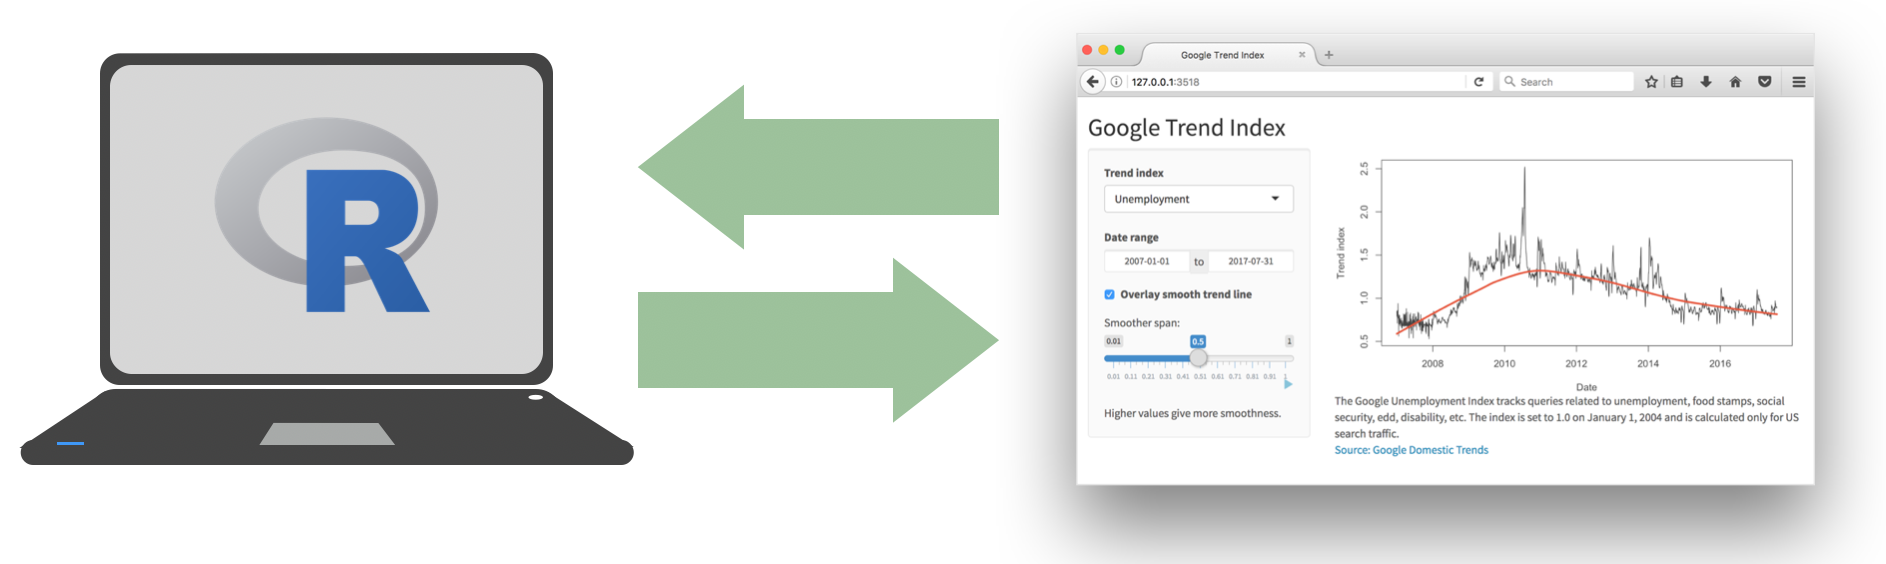
\includegraphics[width=0.8\textwidth,height=\textheight]{./images/recap-2.png}

}

\end{figure}

\hypertarget{section-6}{%
\subsection{}\label{section-6}}

When your app is deployed, the computer serving your app is a web
server.

\begin{figure}

{\centering 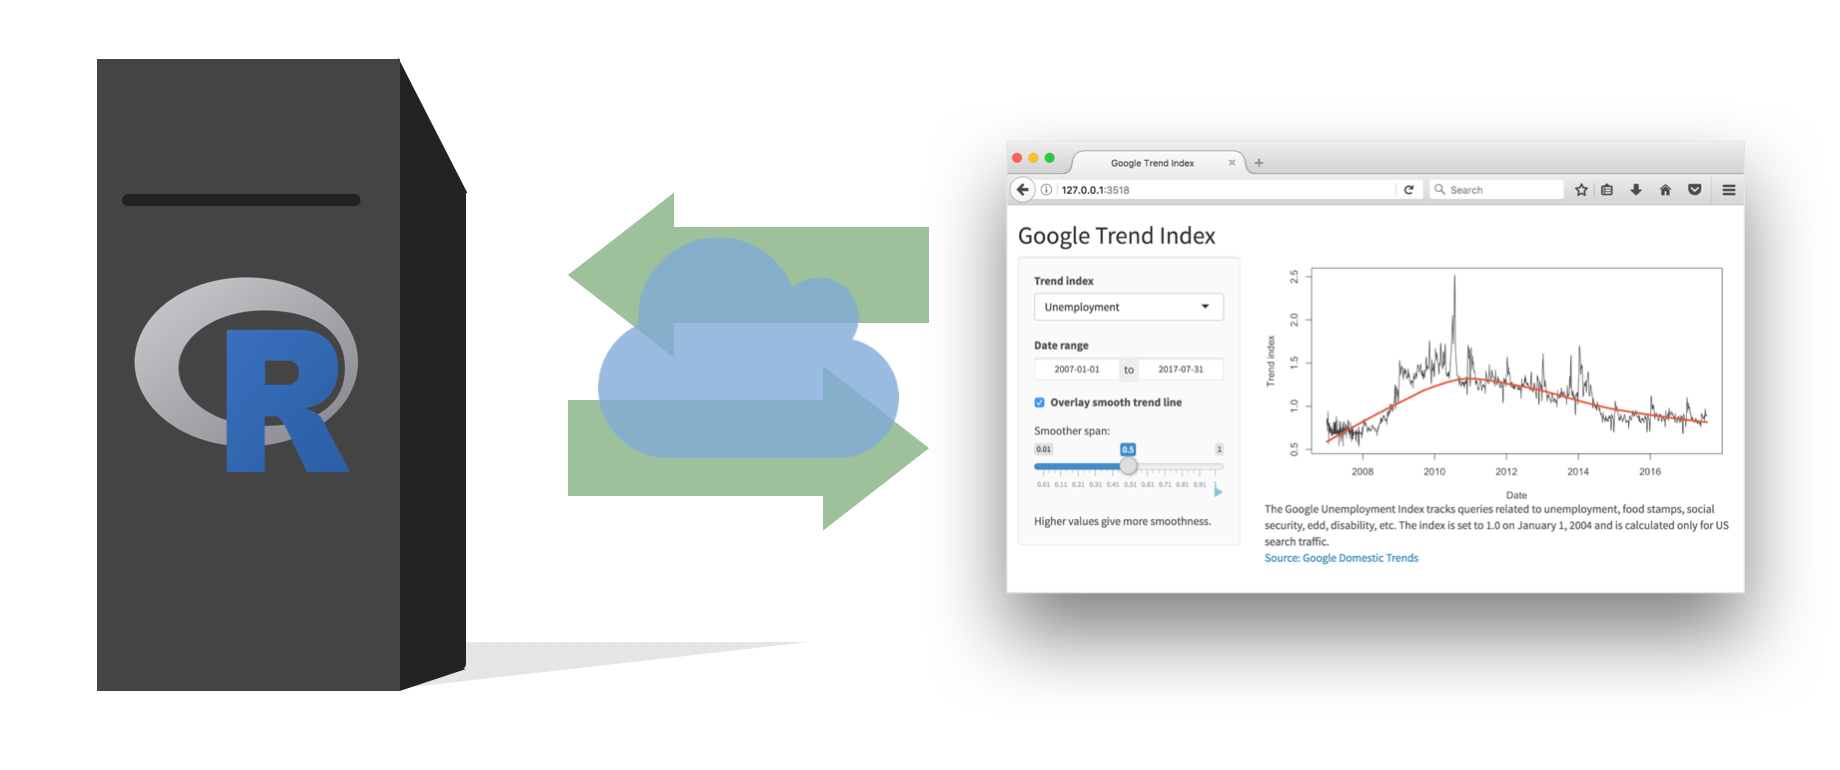
\includegraphics[width=0.8\textwidth,height=\textheight]{./images/recap-3.png}

}

\end{figure}

\hypertarget{section-7}{%
\subsection{}\label{section-7}}

Each app is comprised of two components, a UI and a server.

\begin{figure}

{\centering 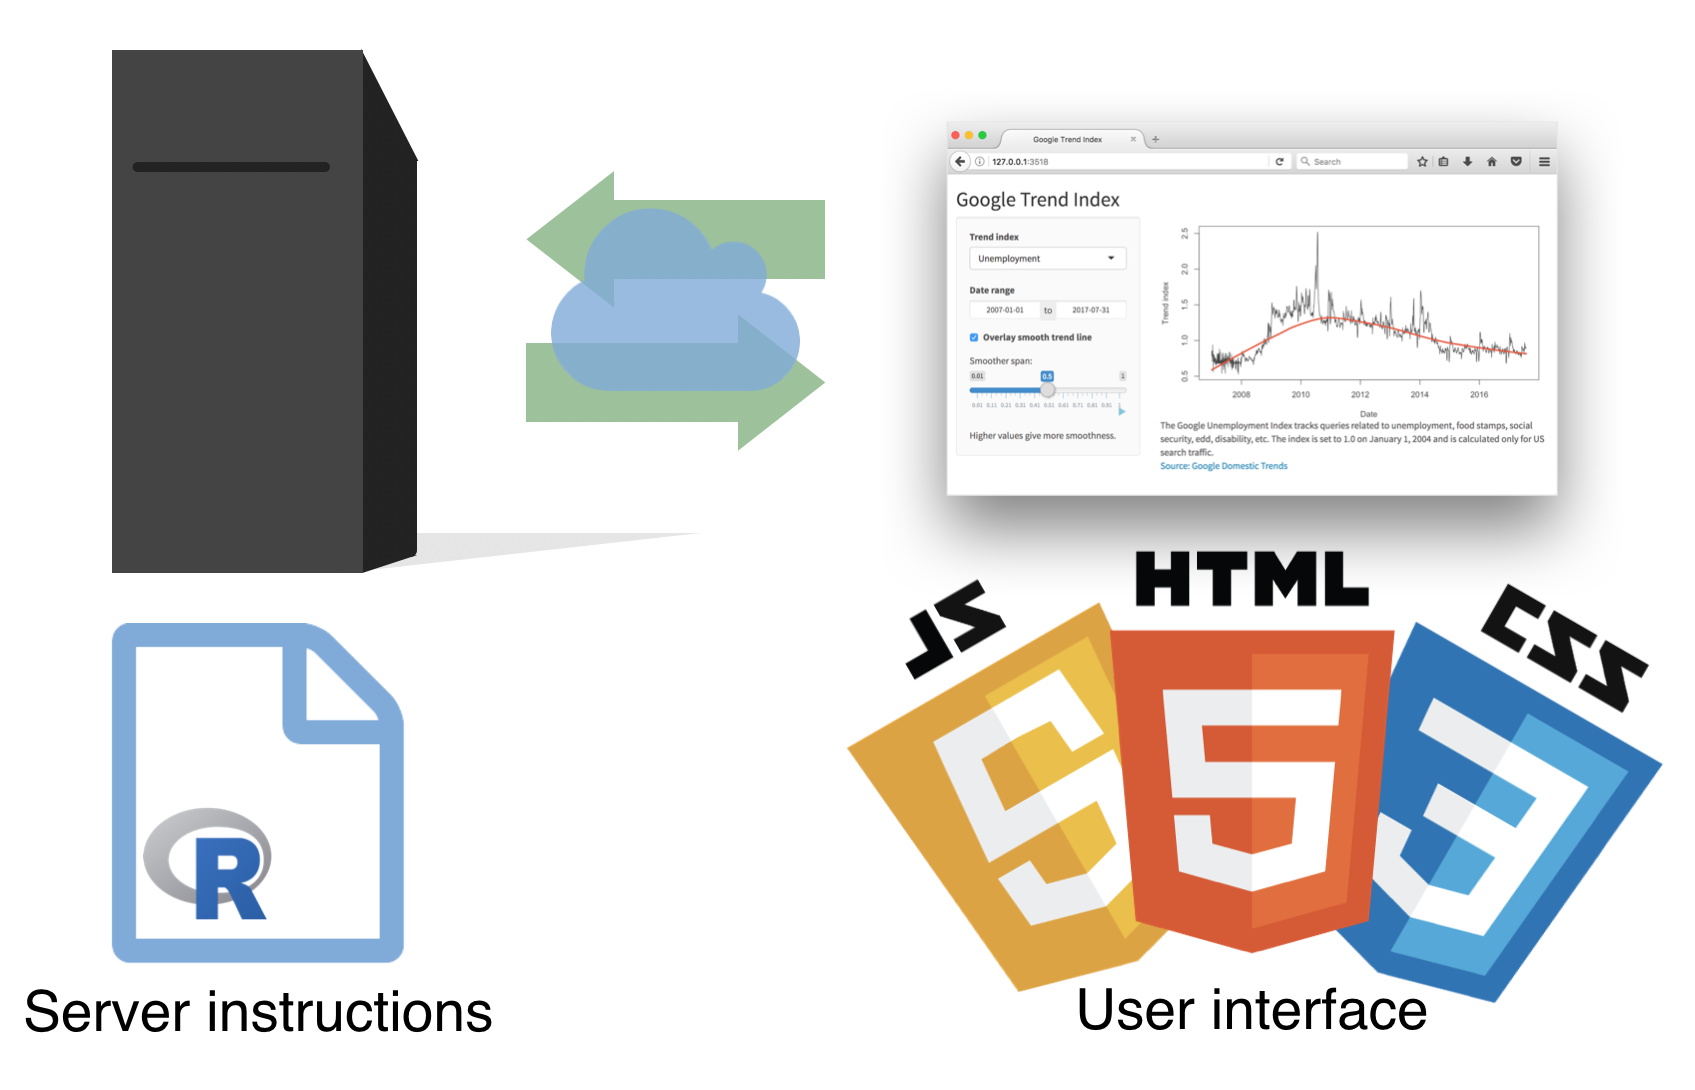
\includegraphics[width=0.8\textwidth,height=\textheight]{./images/recap-4.png}

}

\end{figure}

\begin{itemize}
\item
  The UI is ultimately built with HTML, CSS, and JavaScript. However,
  you as the Shiny developer do not need to know these languages. Shiny
  lets R users write user interfaces using a simple, familiar-looking
  API. However there are no limits to customization for advanced users
  who are familiar with these languages.
\item
  The server function contains the instructions to map user inputs to
  outputs.
\end{itemize}

I often think of the UI as containing syntax specific to Shiny, and the
server as containing R code you might already be familiar with -- with
some Shiny functions added to achieve reactivity.

\hypertarget{tip-change-display}{%
\subsection{Tip: Change display}\label{tip-change-display}}

In this tutorial you will be developing your apps in RStudio Cloud
projects, but once you're done with the tutorial you might consider
developing your apps in the RStudio IDE, which has some some handy-dandy
functionality for running and viewing your apps.

RStudio will automatically recognize R scripts that contain \texttt{ui}
and \texttt{server} components and that end with a call to the
\texttt{shinyApp()} function and will make available the Run App button.
You can choose to run your app in a new window, or in the viewer pane of
your RStudio window.

\begin{figure}

{\centering 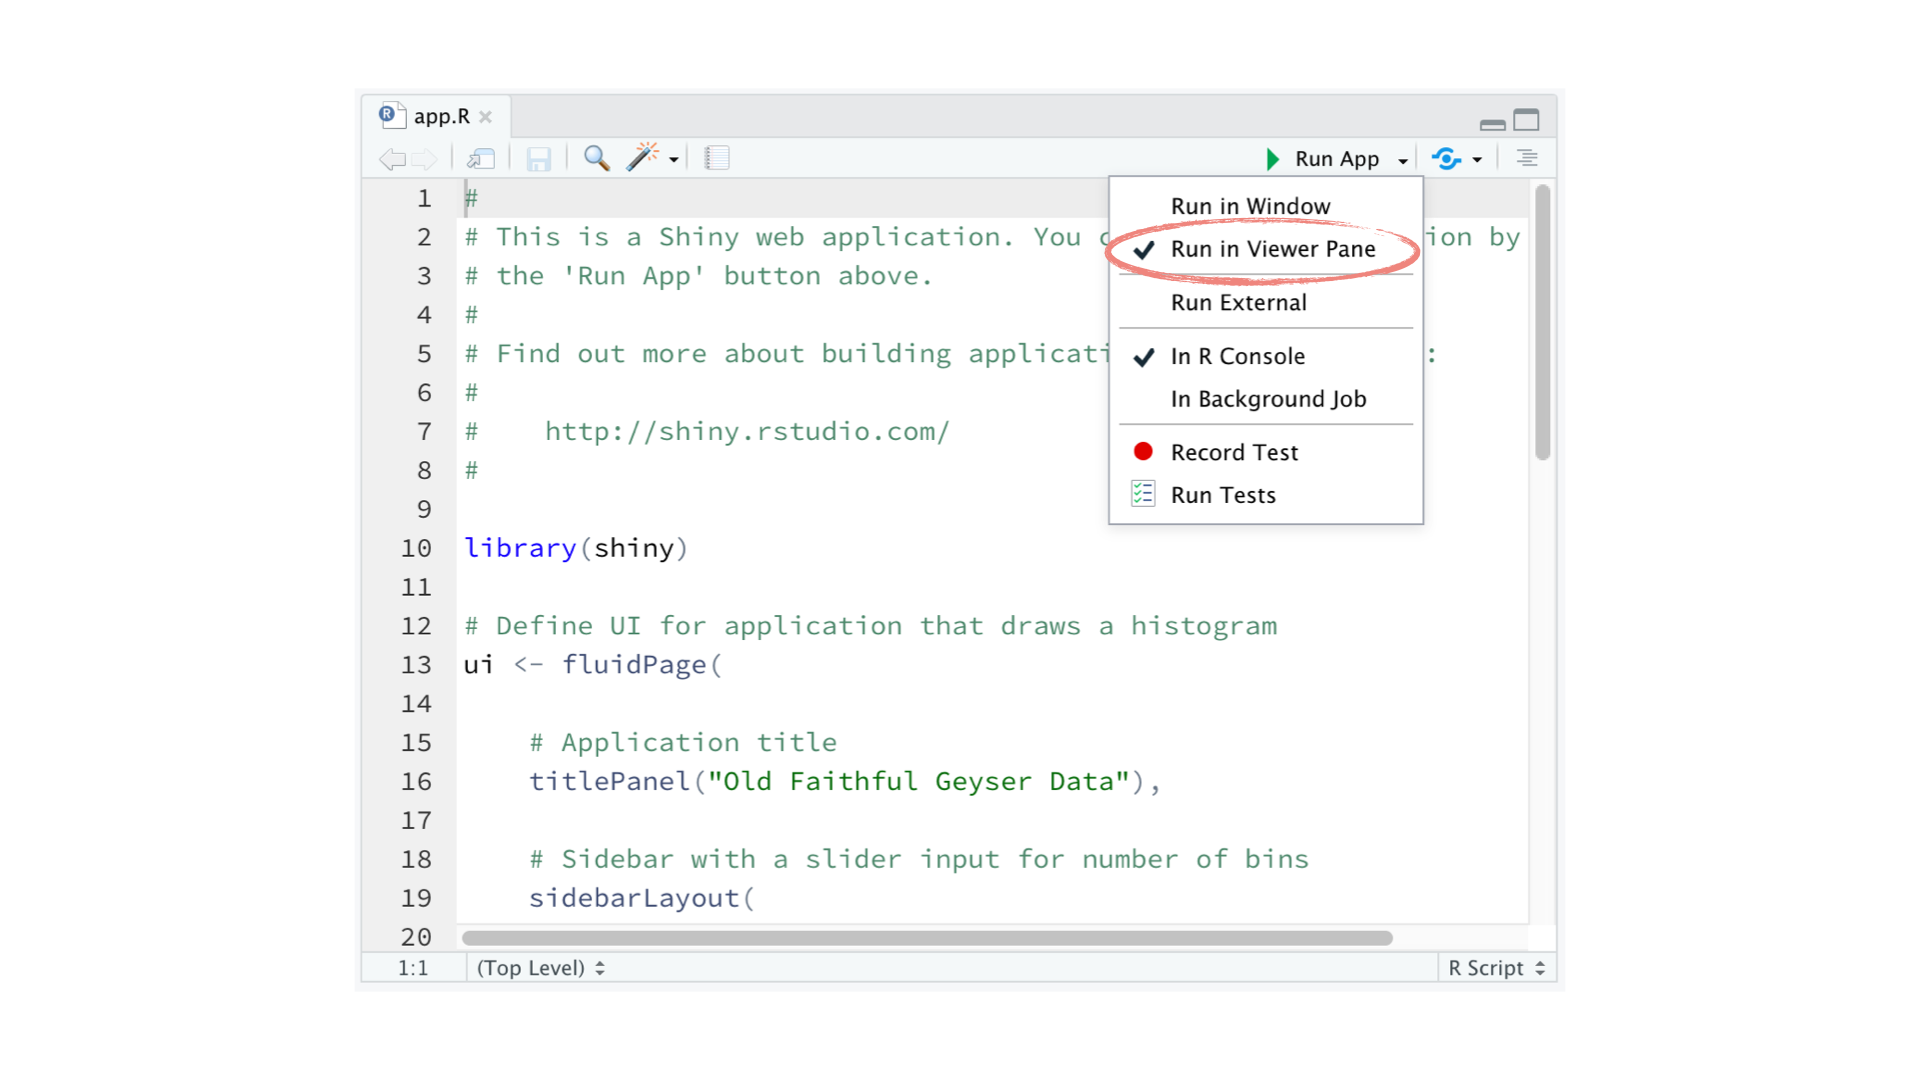
\includegraphics[width=0.8\textwidth,height=\textheight]{./images/recap-5.png}

}

\end{figure}

\hypertarget{tip-close-an-app}{%
\subsection{Tip: Close an app}\label{tip-close-an-app}}

When you are done with an app, you can terminate the session by clicking
the red stop button in your viewer pane.

\begin{figure}

{\centering 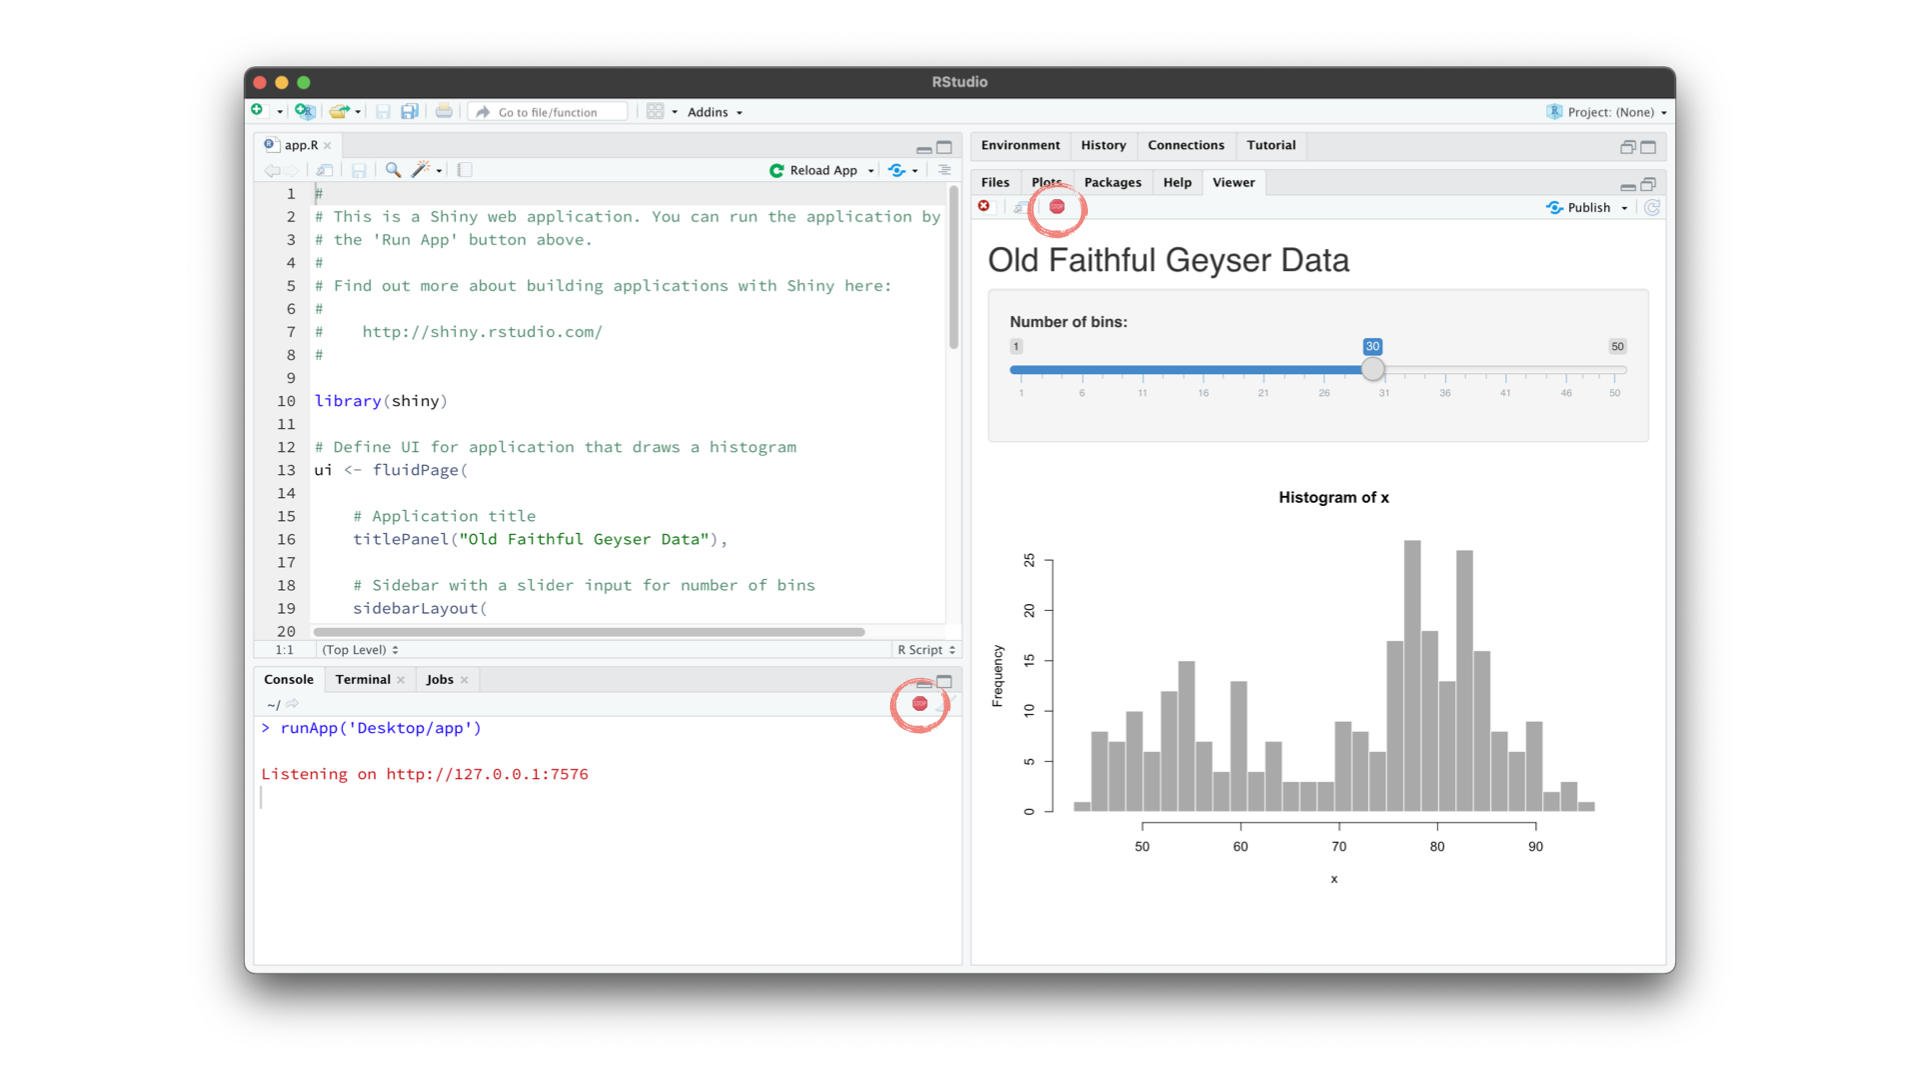
\includegraphics[width=0.8\textwidth,height=\textheight]{./images/recap-6.png}

}

\end{figure}

\hypertarget{section-8}{%
\subsection{}\label{section-8}}

That's all for this module! In the next module we discuss inputs,
outputs, and rendering functions in further detail.

\hypertarget{user-interface-ui-1}{%
\chapter{User interface (UI)}\label{user-interface-ui-1}}

In this section we'll build the user interface of a simple app.

However, before we get into the weeds of building a user interface,
let's revisit the anatomy of a Shiny app.

\begin{figure}

{\centering 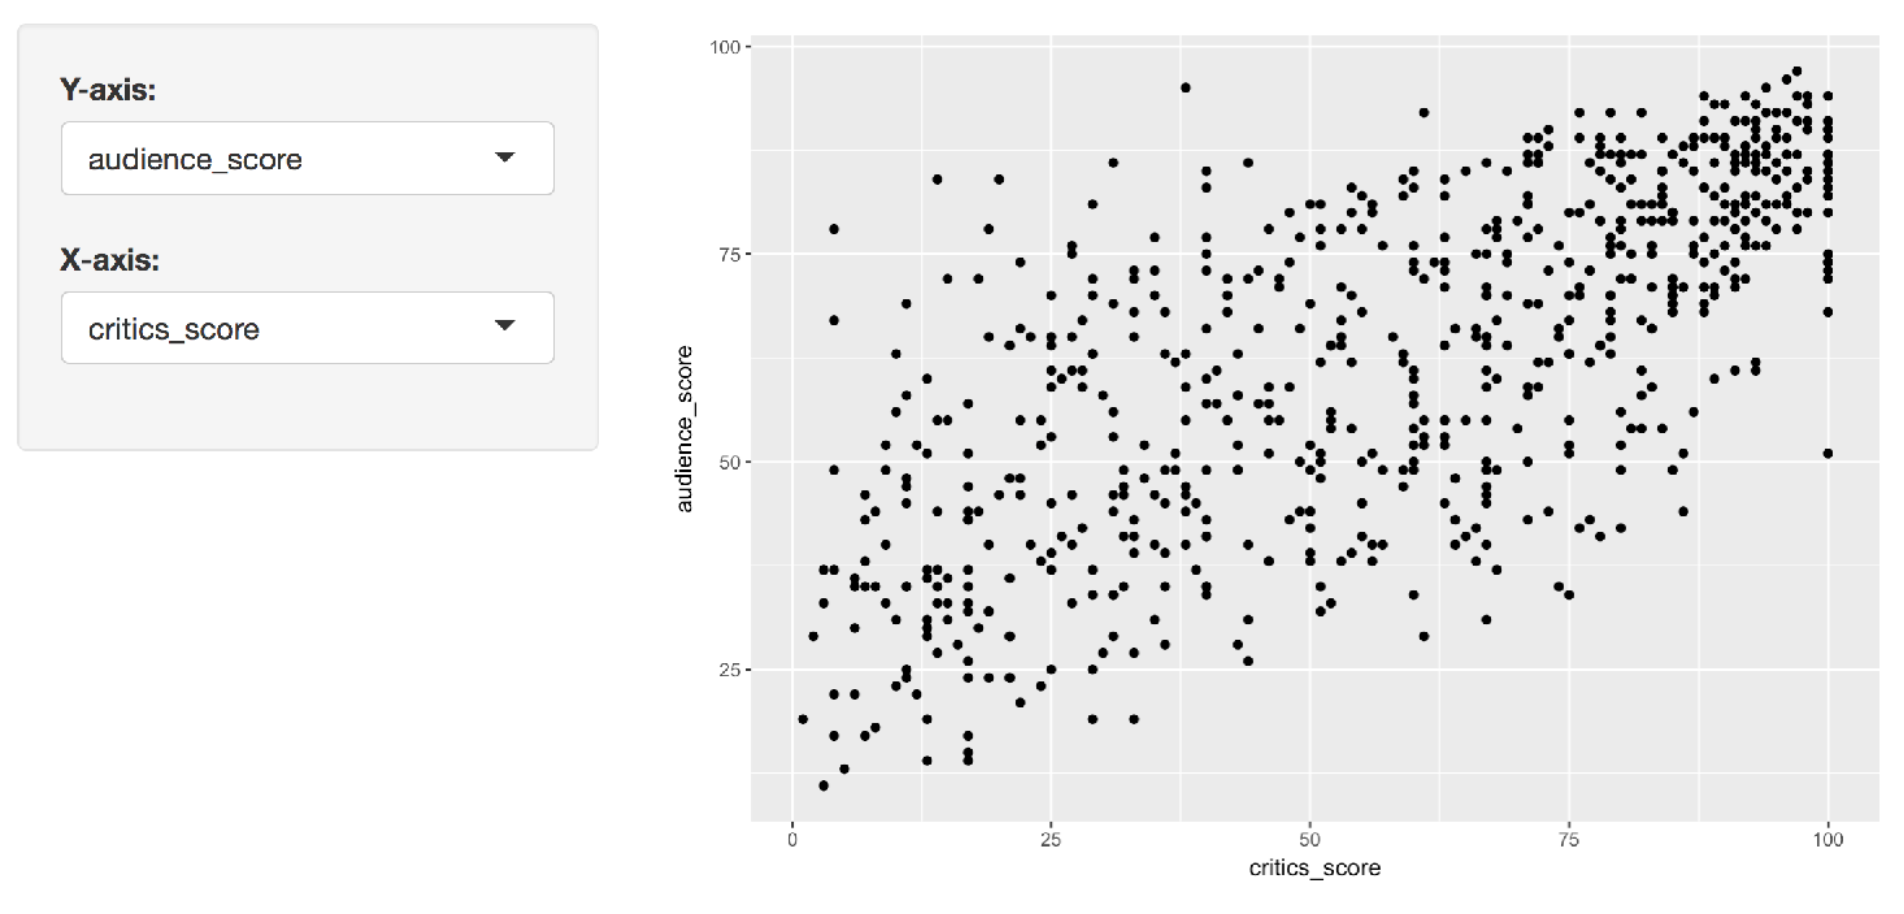
\includegraphics[width=1\textwidth,height=\textheight]{./images/app-selectinput-scatterplot.png}

}

\end{figure}

\begin{itemize}
\item
  The user interface, that we'll refer to as the ``UI'' going forward,
  defines and lays out the inputs of your app where users can make their
  selections. It also lays out the outputs.
\item
  The server function, on the other hand, calculates outputs and
  performs any other calculations needed for the outputs.
\end{itemize}

\hypertarget{example-1}{%
\subsection{Example}\label{example-1}}

\begin{figure}

{\centering 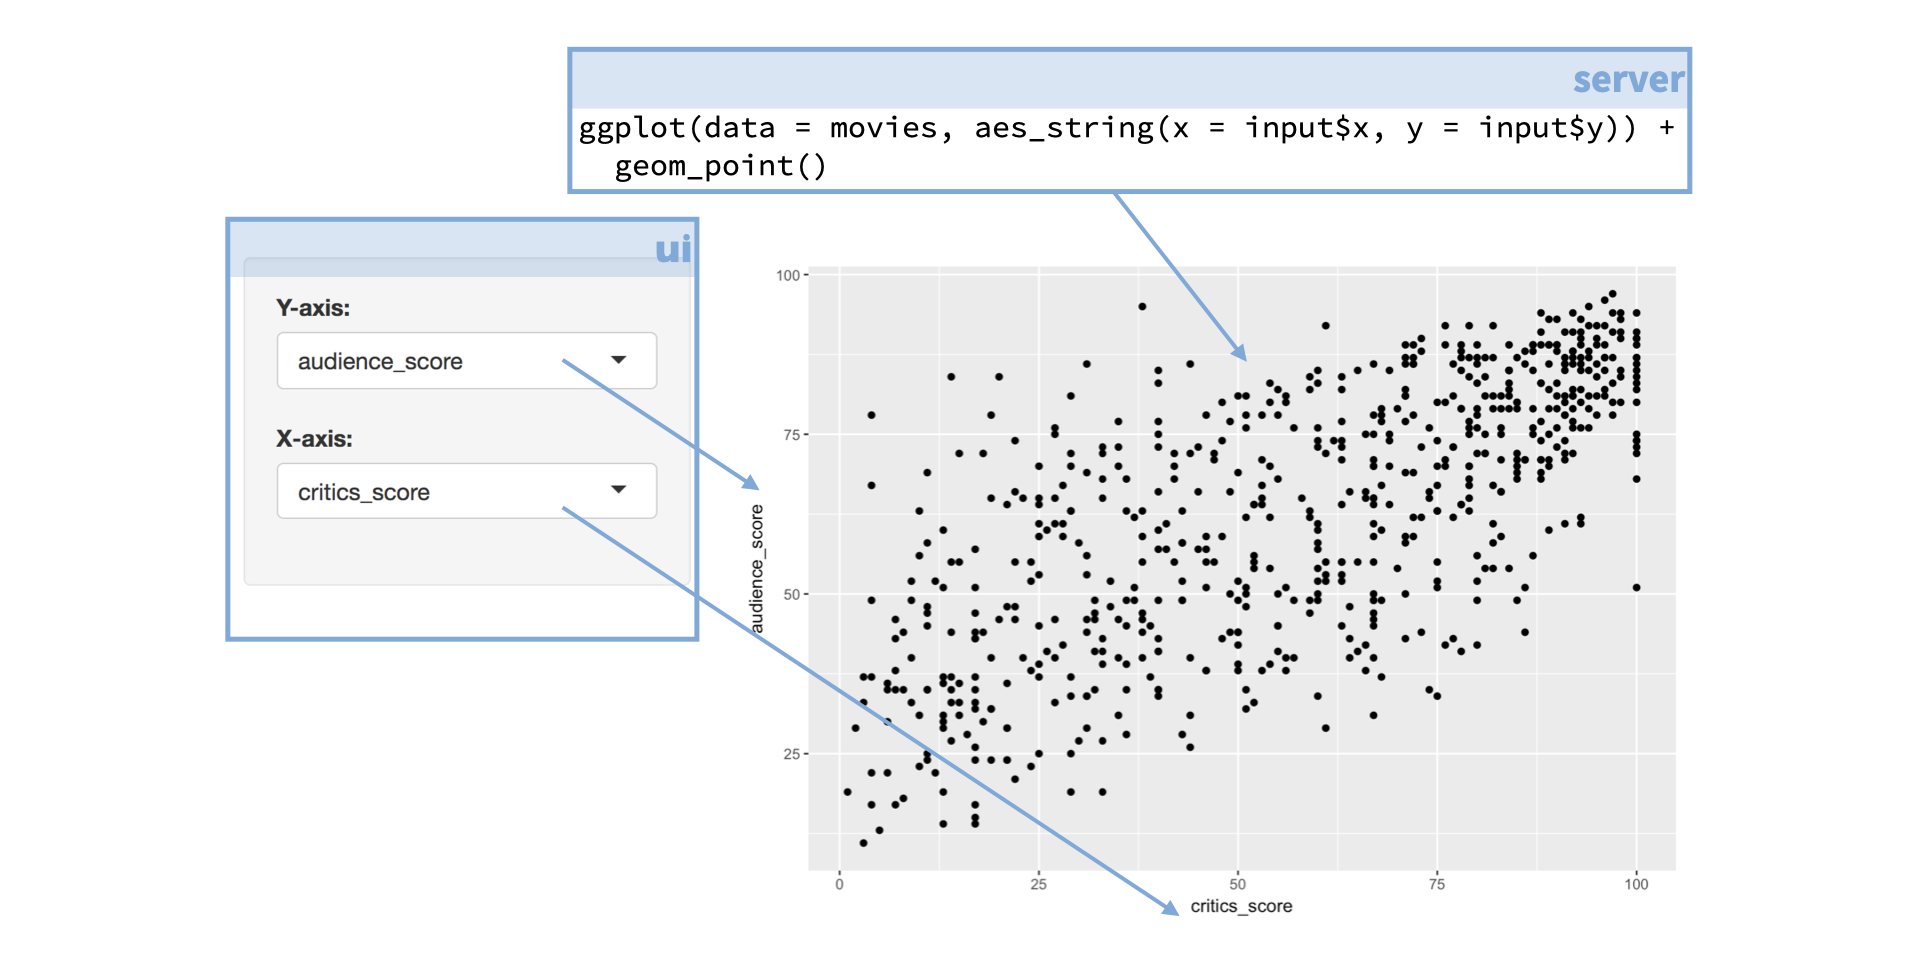
\includegraphics[width=1\textwidth,height=\textheight]{./images/ui-to-scatterplot.png}

}

\end{figure}

For example, if your app features a plot the code for building that plot
lives in the server function. But the setup for the user defined inputs
for the plot, as well as information on where physically on the app the
plot should appear, are defined in the UI.

\hypertarget{section-9}{%
\subsection{}\label{section-9}}

Here is the app we'll work with in this section and the code that builds
the UI of that app.

Since this is too much code to parse, we'll explore individual
components of the UI one by one.

\begin{figure}

{\centering 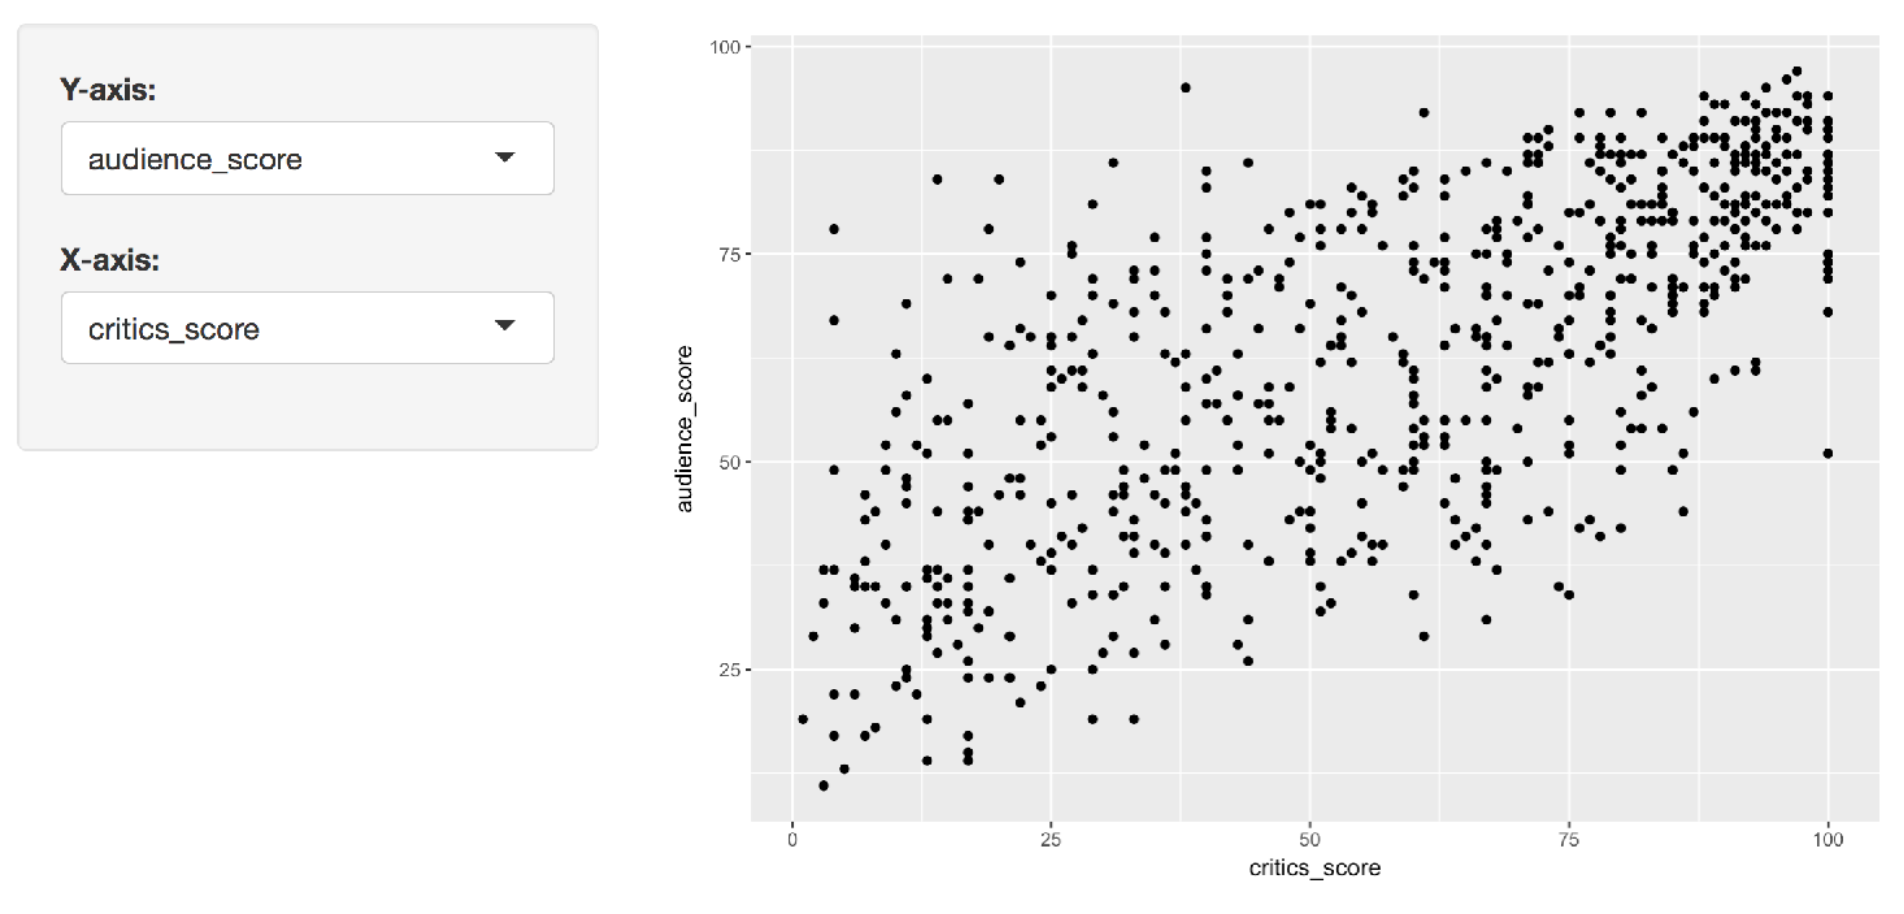
\includegraphics[width=1\textwidth,height=\textheight]{./images/app-selectinput-scatterplot.png}

}

\end{figure}

\begin{figure}

{\centering 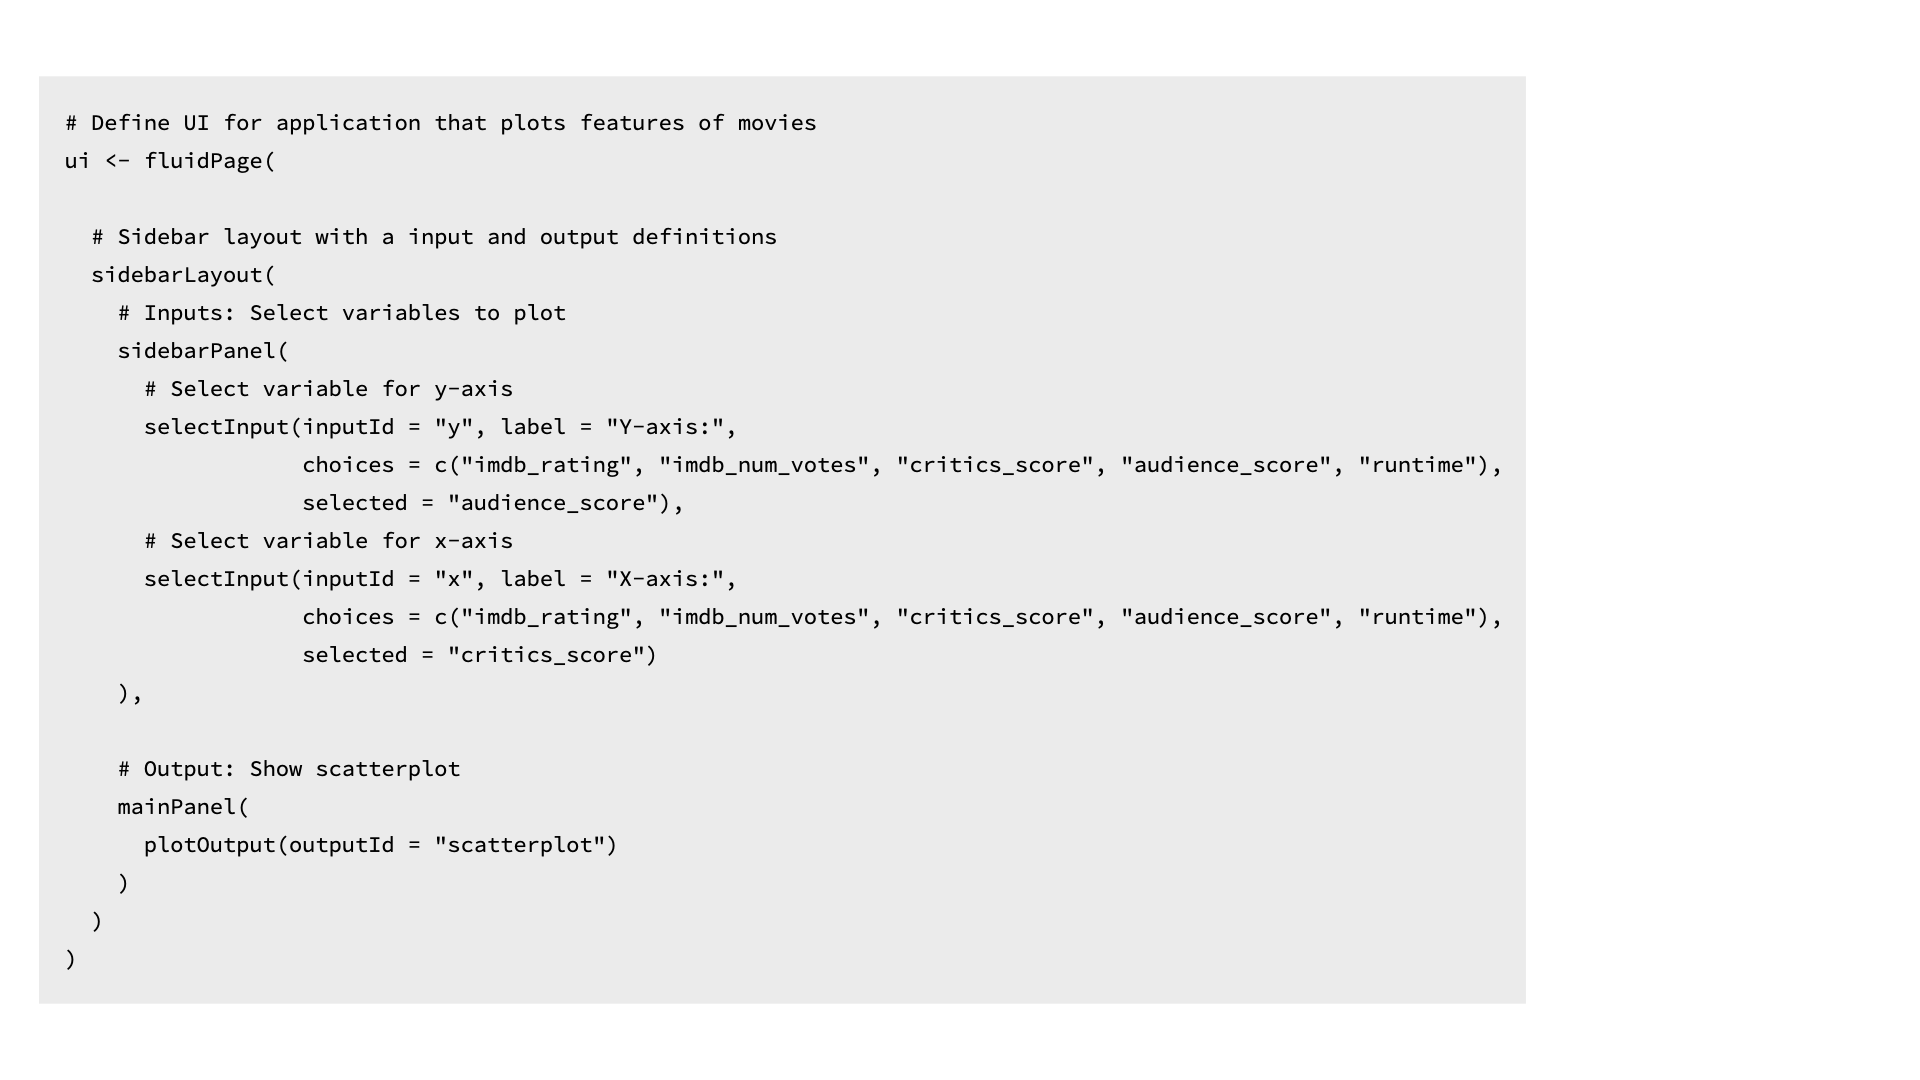
\includegraphics[width=1\textwidth,height=\textheight]{./images/ui-selectinput-scatterplot.png}

}

\end{figure}

\hypertarget{fluidpage-1}{%
\subsection{\texorpdfstring{\texttt{fluidPage()}}{fluidPage()}}\label{fluidpage-1}}

At the outermost layer of our UI definition we begin with the
\texttt{fluidPage()} function.

\begin{figure}

{\centering 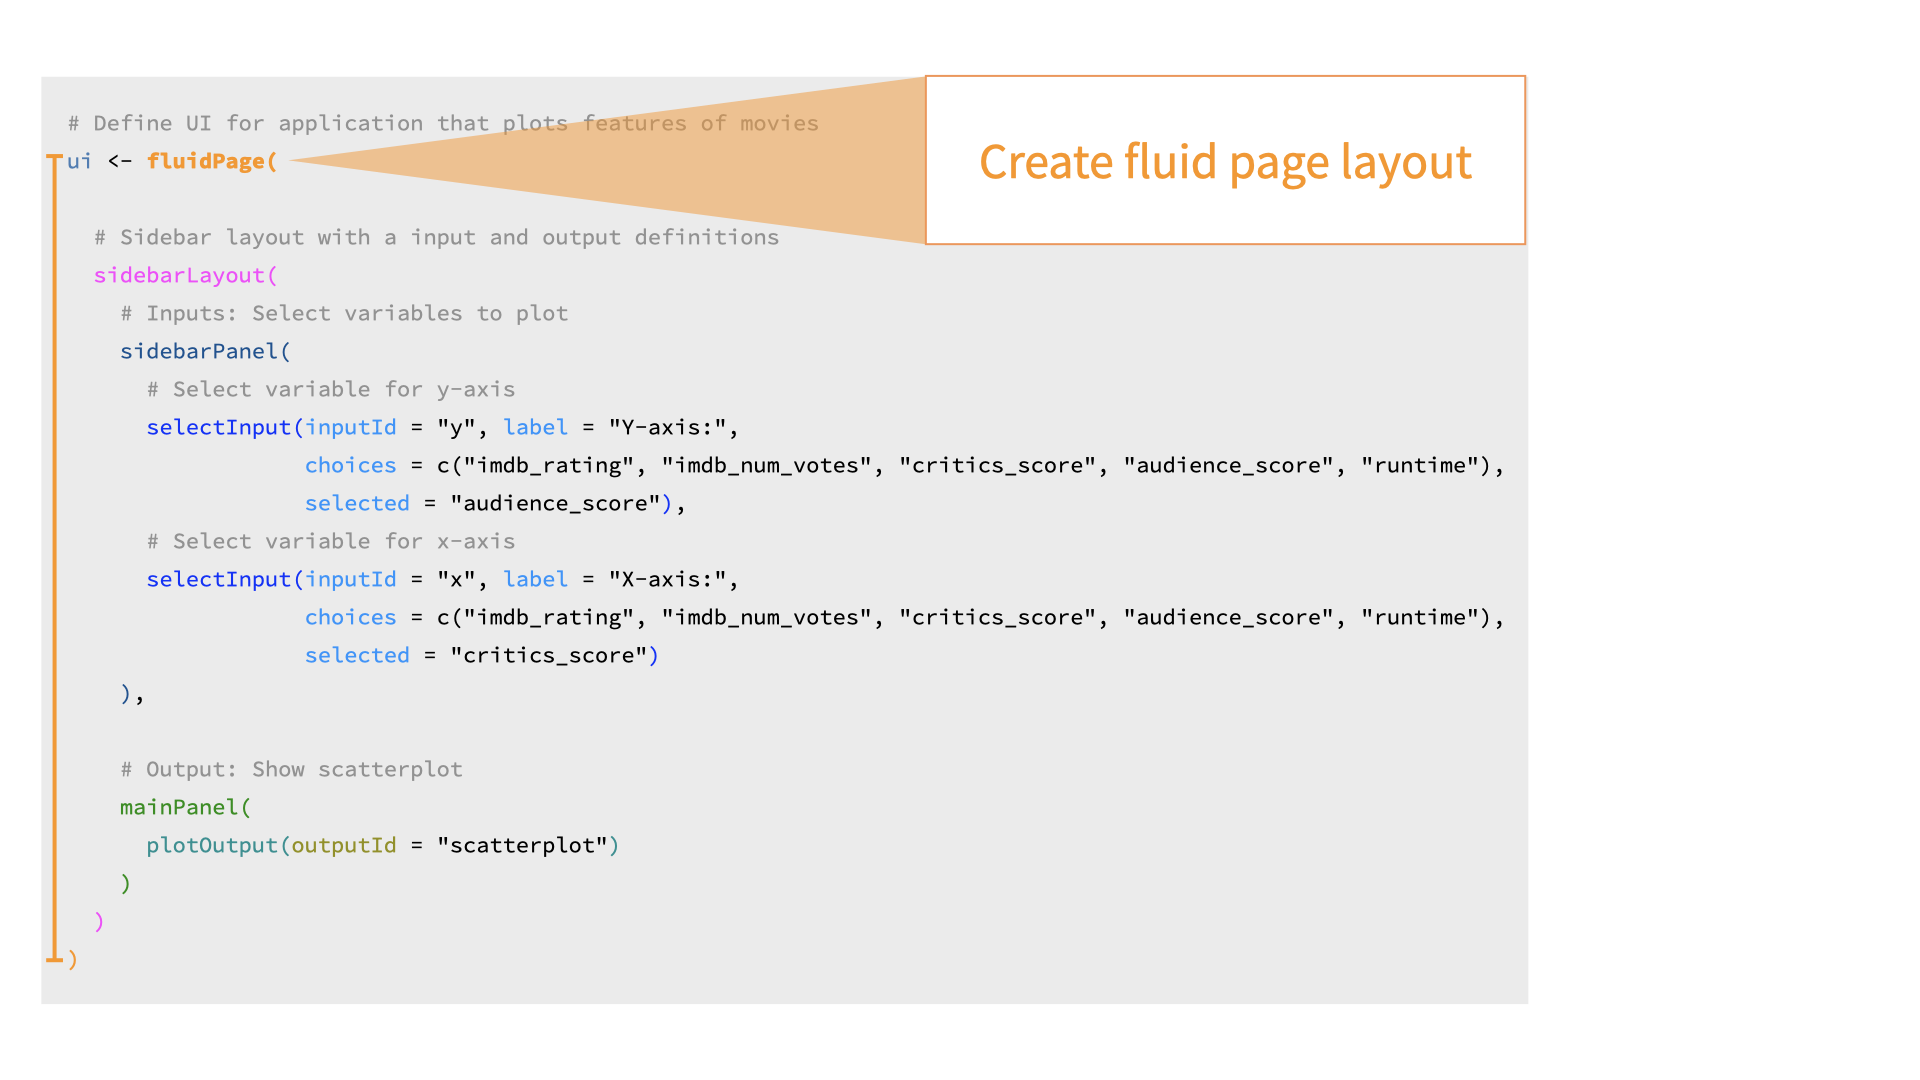
\includegraphics[width=1\textwidth,height=\textheight]{./images/fluidPage.png}

}

\end{figure}

The \texttt{fluidPage()} function creates a fluid page layout consisting
of rows and columns. Rows make sure that elements in them appear on the
same line. Columns within these rows define how much horizontal space
each element should occupy.

Fluid pages scale their components in realtime to fill all available
browser width, which means you, the app developer, don't need to worry
about defining relative widths for individual app components.

As always, for more information on arguments to this function, you can
view the R function help by typing \texttt{?fluidPage} in your R console
or visiting the function reference page on the package website
\href{https://shiny.rstudio.com/reference/shiny/latest/}{here}.

\hypertarget{layout-1}{%
\subsection{Layout}\label{layout-1}}

Next, we define the layout of our app with \texttt{sidebarLayout()}.

\begin{figure}

{\centering 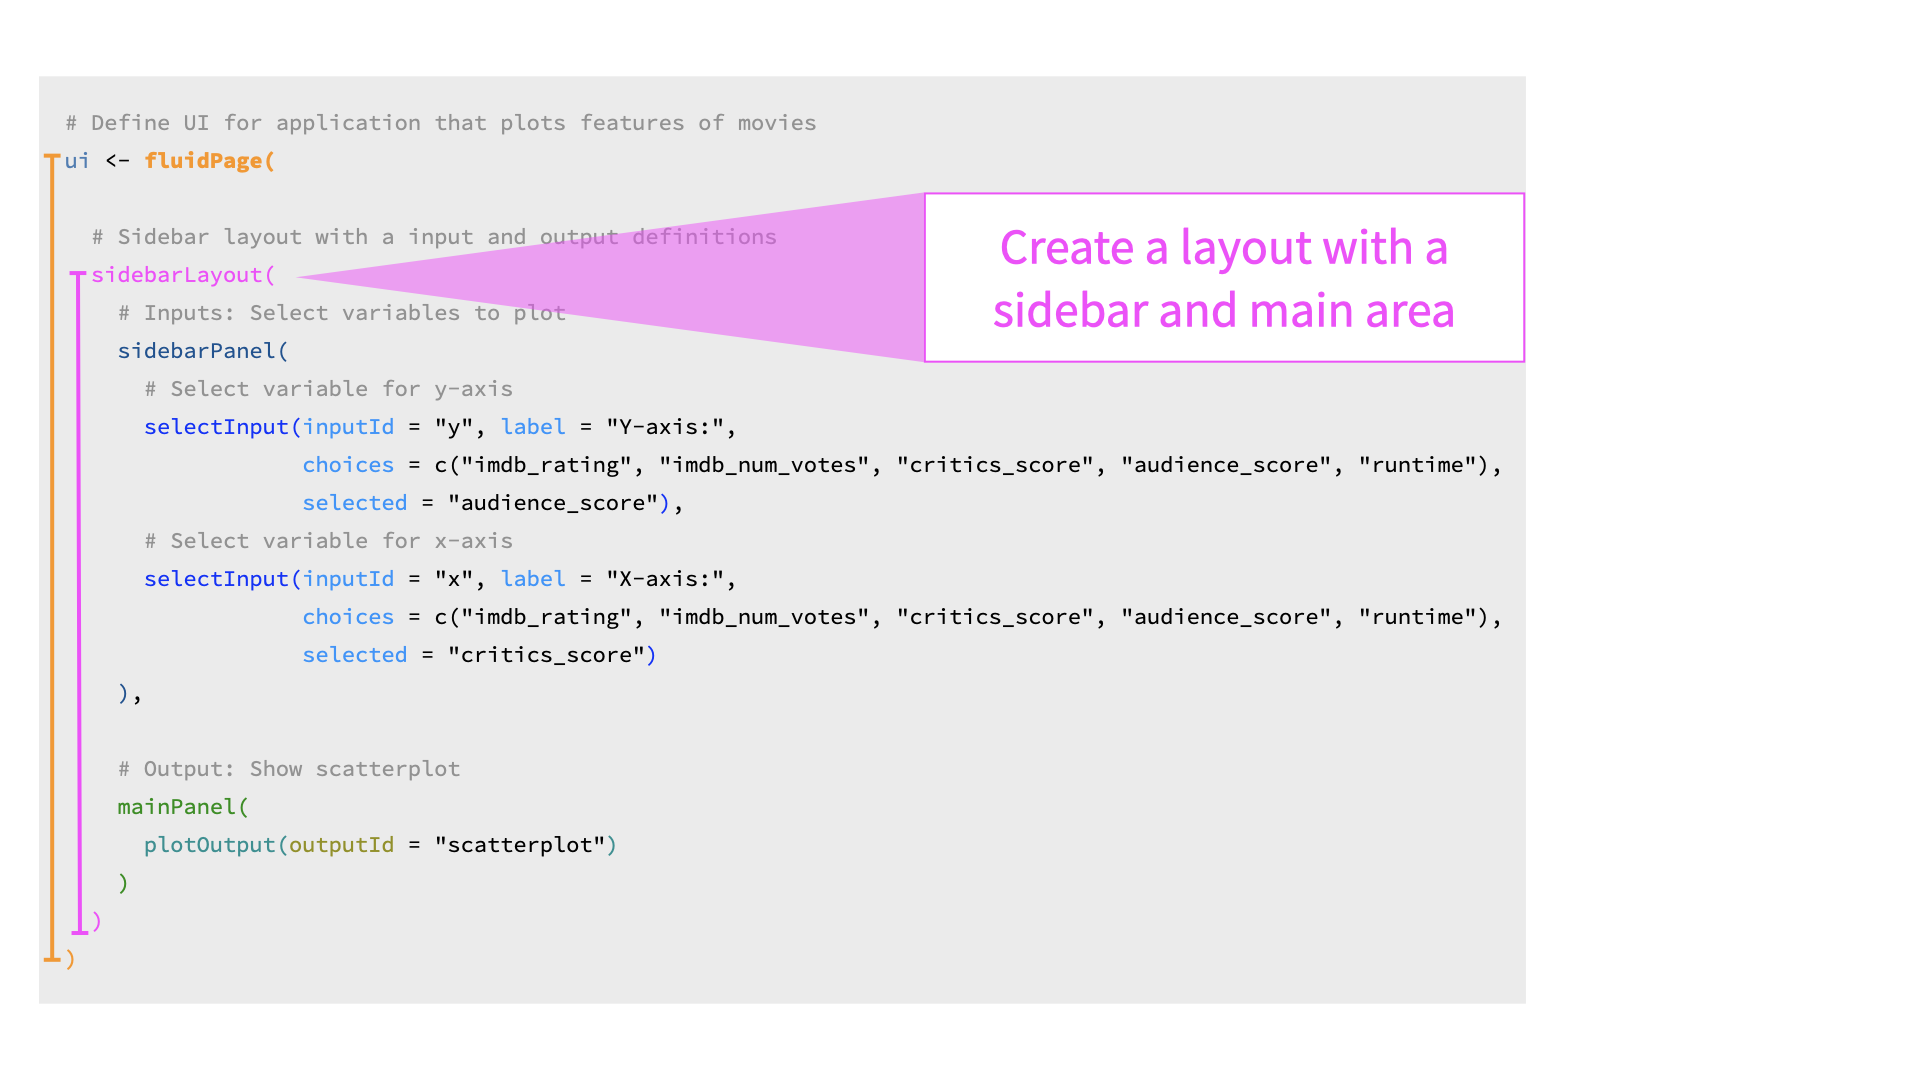
\includegraphics[width=1\textwidth,height=\textheight]{./images/layout.png}

}

\end{figure}

Shiny includes a number of options for laying out the components of an
application. The default layout, the one we're using in our example app,
is a layout with a sidebar, that you can define with the
\texttt{sidebarLayout()} function.

\begin{figure}

{\centering 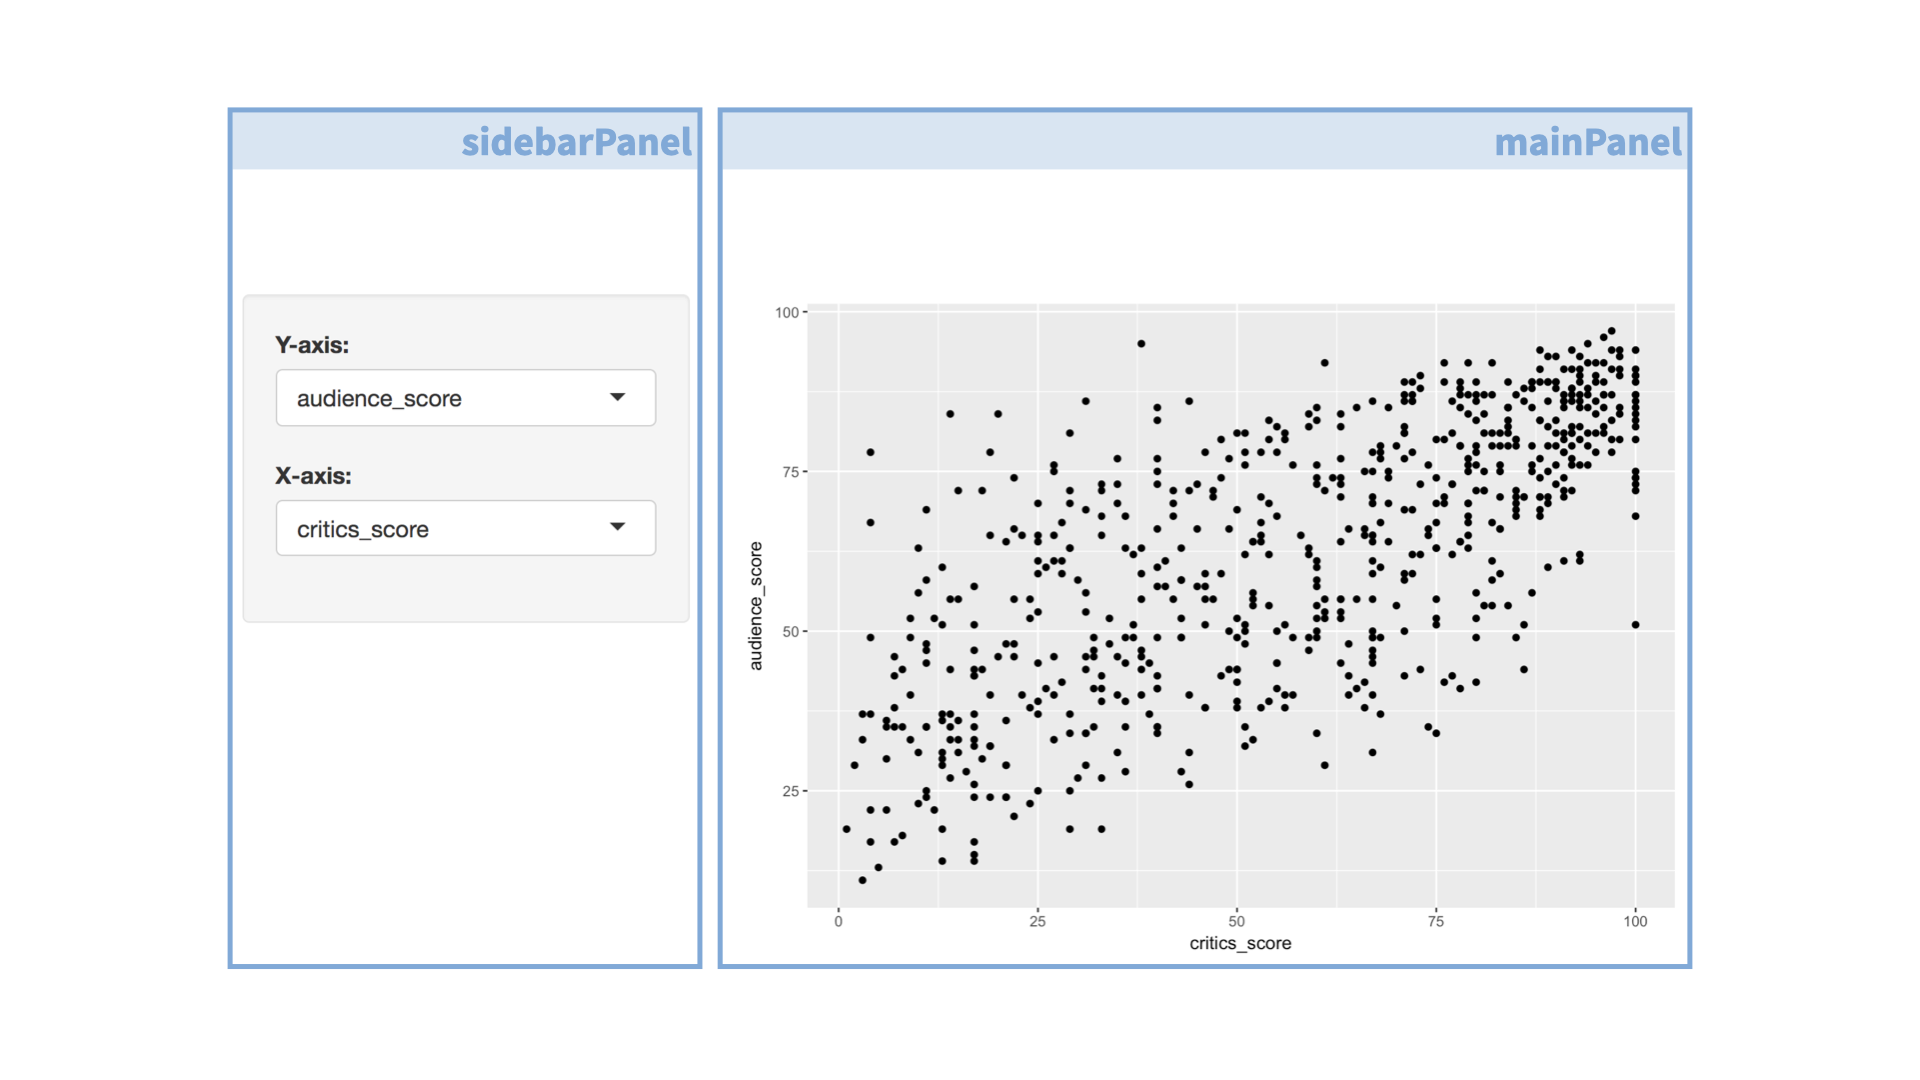
\includegraphics[width=1\textwidth,height=\textheight]{./images/layout-app.png}

}

\end{figure}

This is a simple layout with a narrow sidebar for inputs and a wider
main area for output.

Under the hood, Shiny implements layout features available in Bootstrap
2, which is a popular HTML/CSS framework. However the nice thing about
working in Shiny is that no prior experience with Bootstrap is
necessary.

To learn more about various layouts, I recommend reviewing the
\href{https://shiny.rstudio.com/articles/layout-guide.html}{Application
Layout Guide article} at \url{shiny.rstudio.com}.

\hypertarget{input-controls-1}{%
\subsection{Input controls}\label{input-controls-1}}

Next we define our sidebar panel containing input controls.

\begin{figure}

{\centering 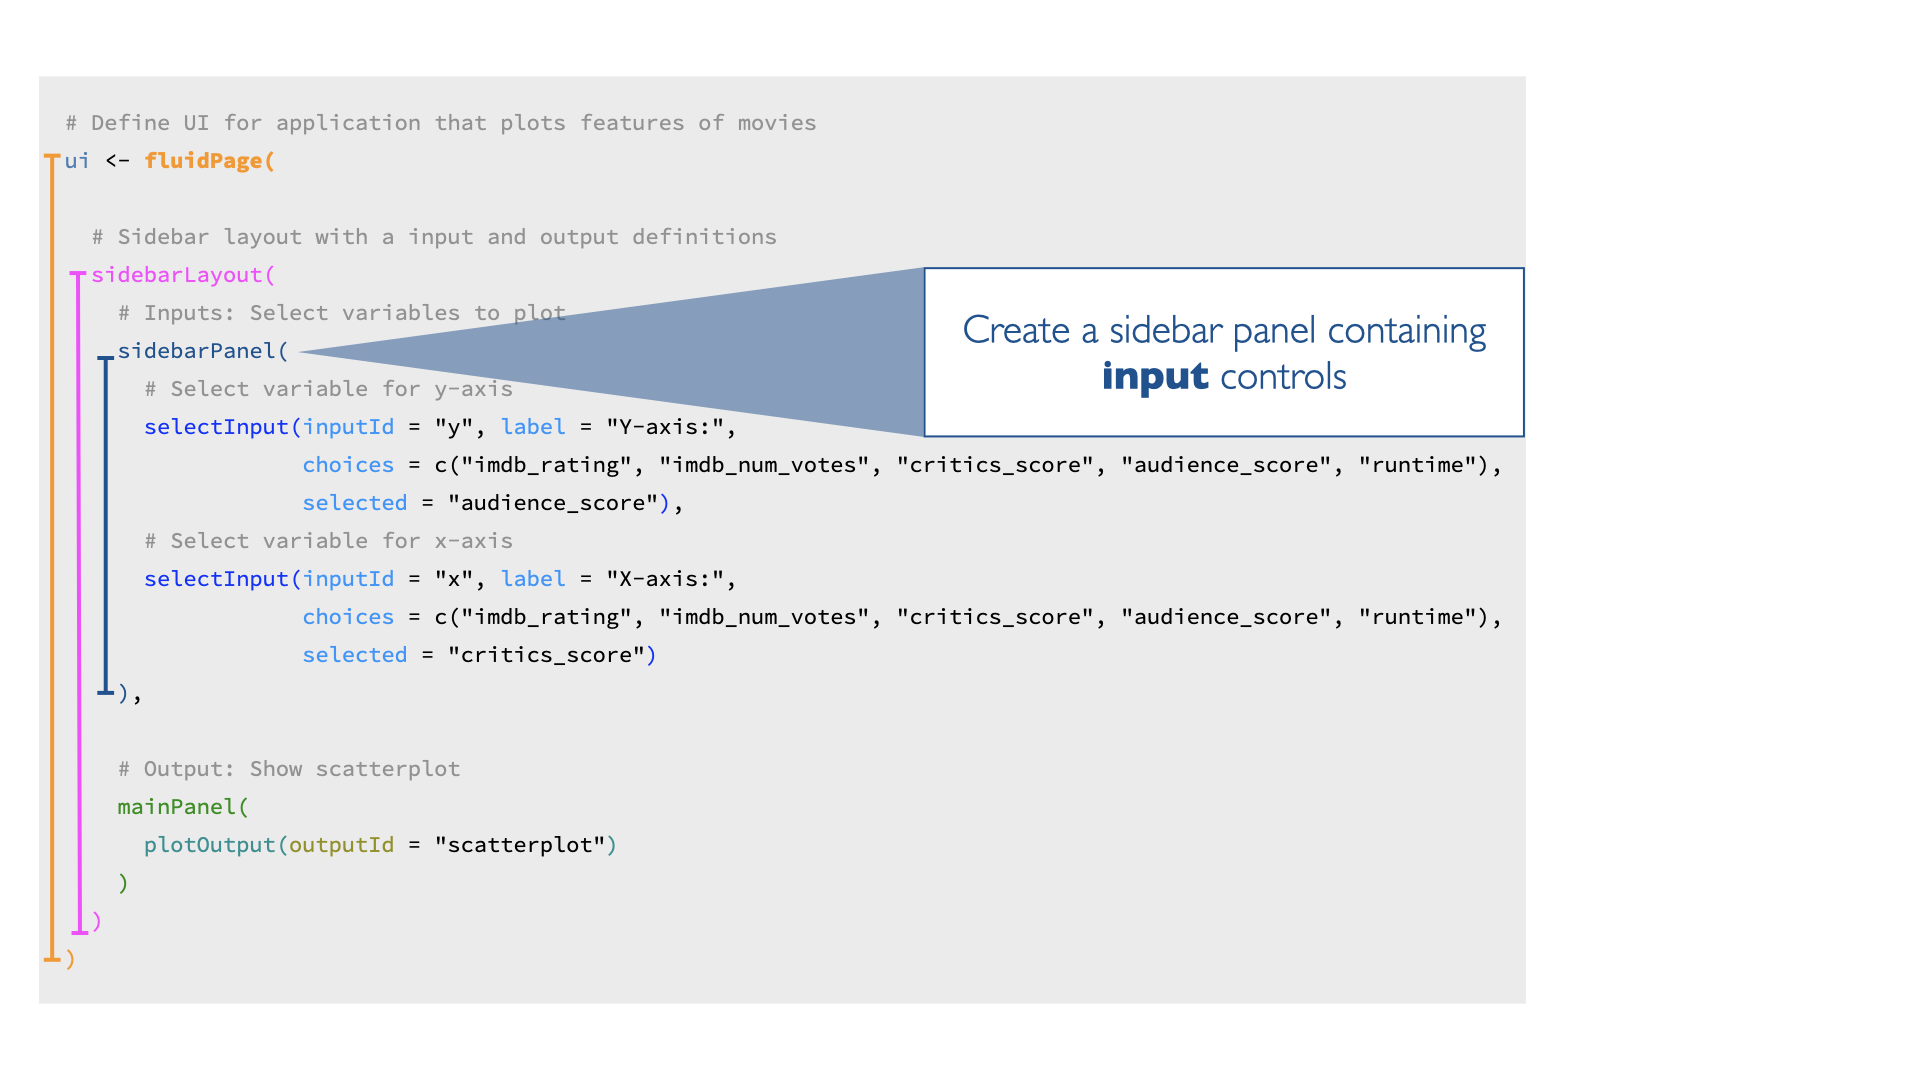
\includegraphics[width=1\textwidth,height=\textheight]{./images/input-controls.png}

}

\end{figure}

\hypertarget{section-10}{%
\subsection{}\label{section-10}}

This panel contains two dropdown menus created with the
\texttt{selectInput()} function.

\begin{figure}

{\centering 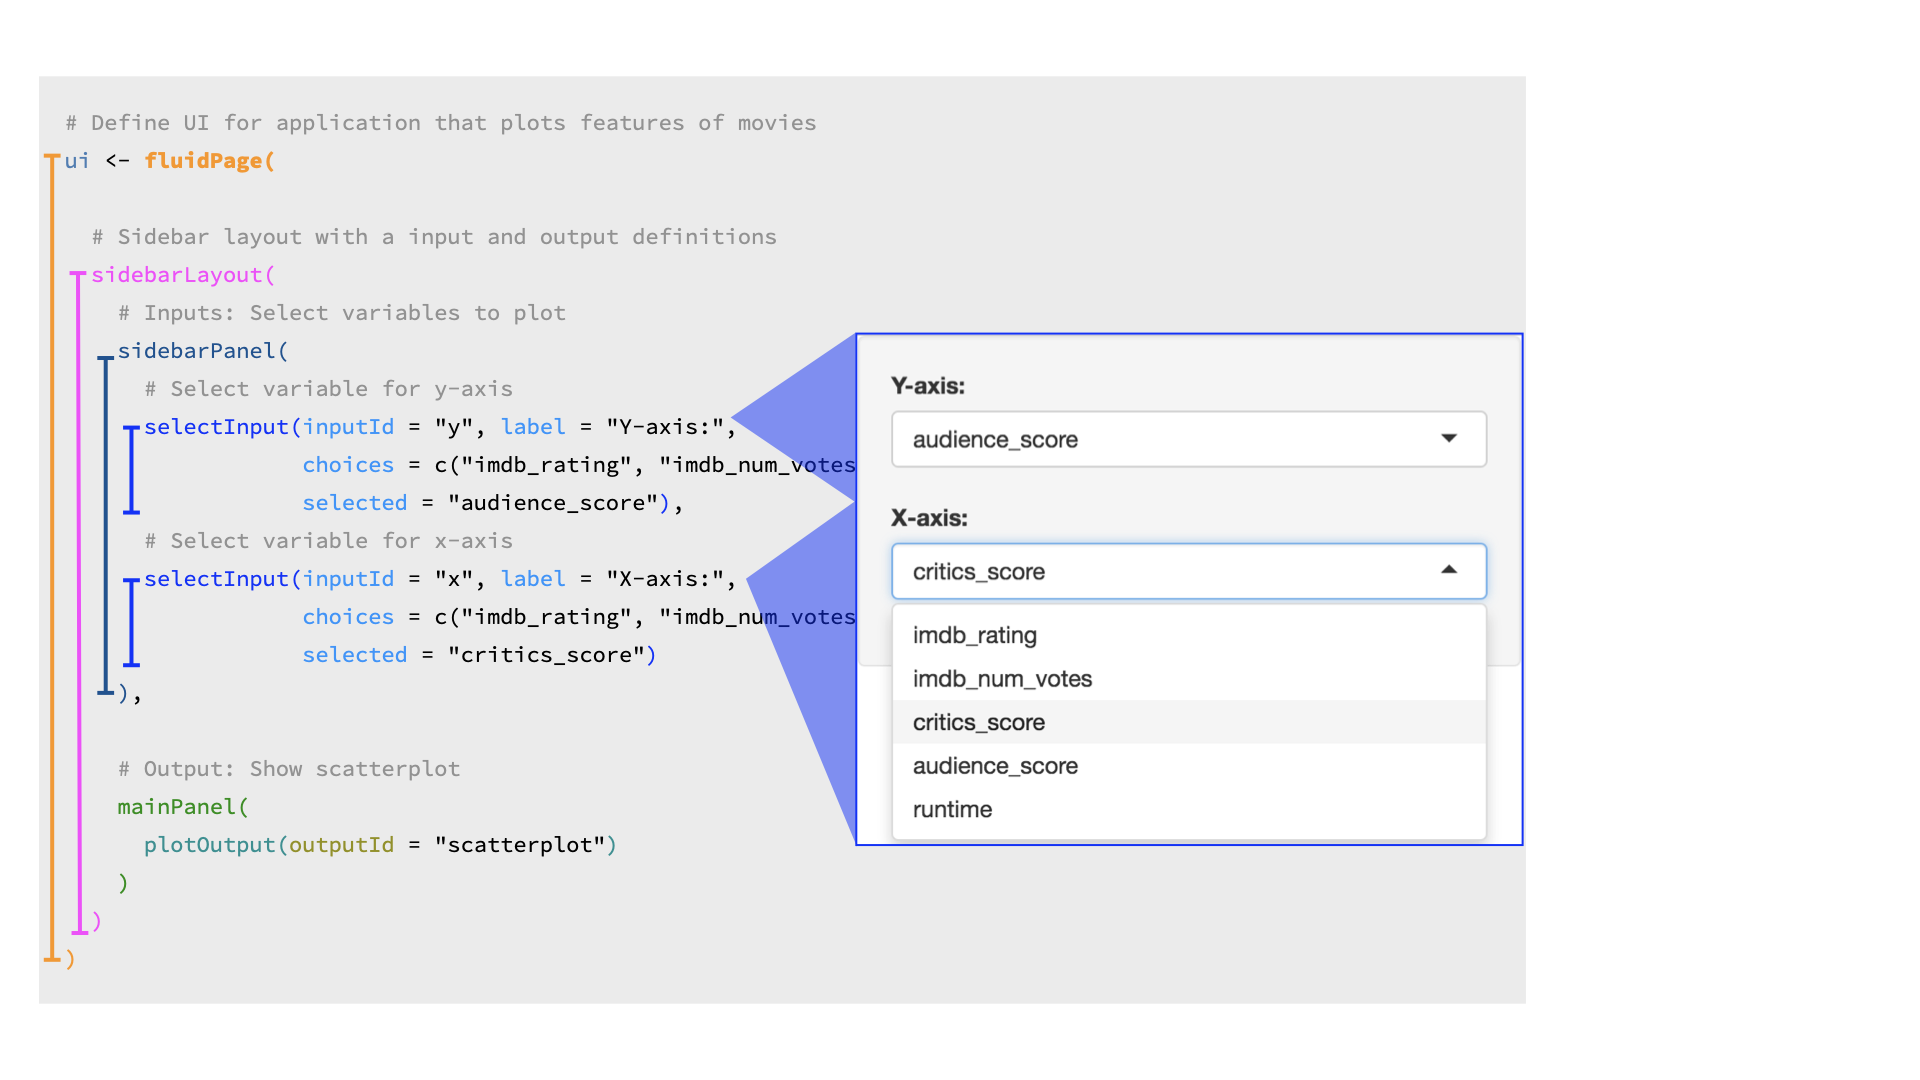
\includegraphics[width=1\textwidth,height=\textheight]{./images/input-dropdowns.png}

}

\end{figure}

\hypertarget{section-11}{%
\subsection{}\label{section-11}}

Let's take a look at one of the \texttt{selectInput} widgets a little
more closely.

\begin{figure}

{\centering 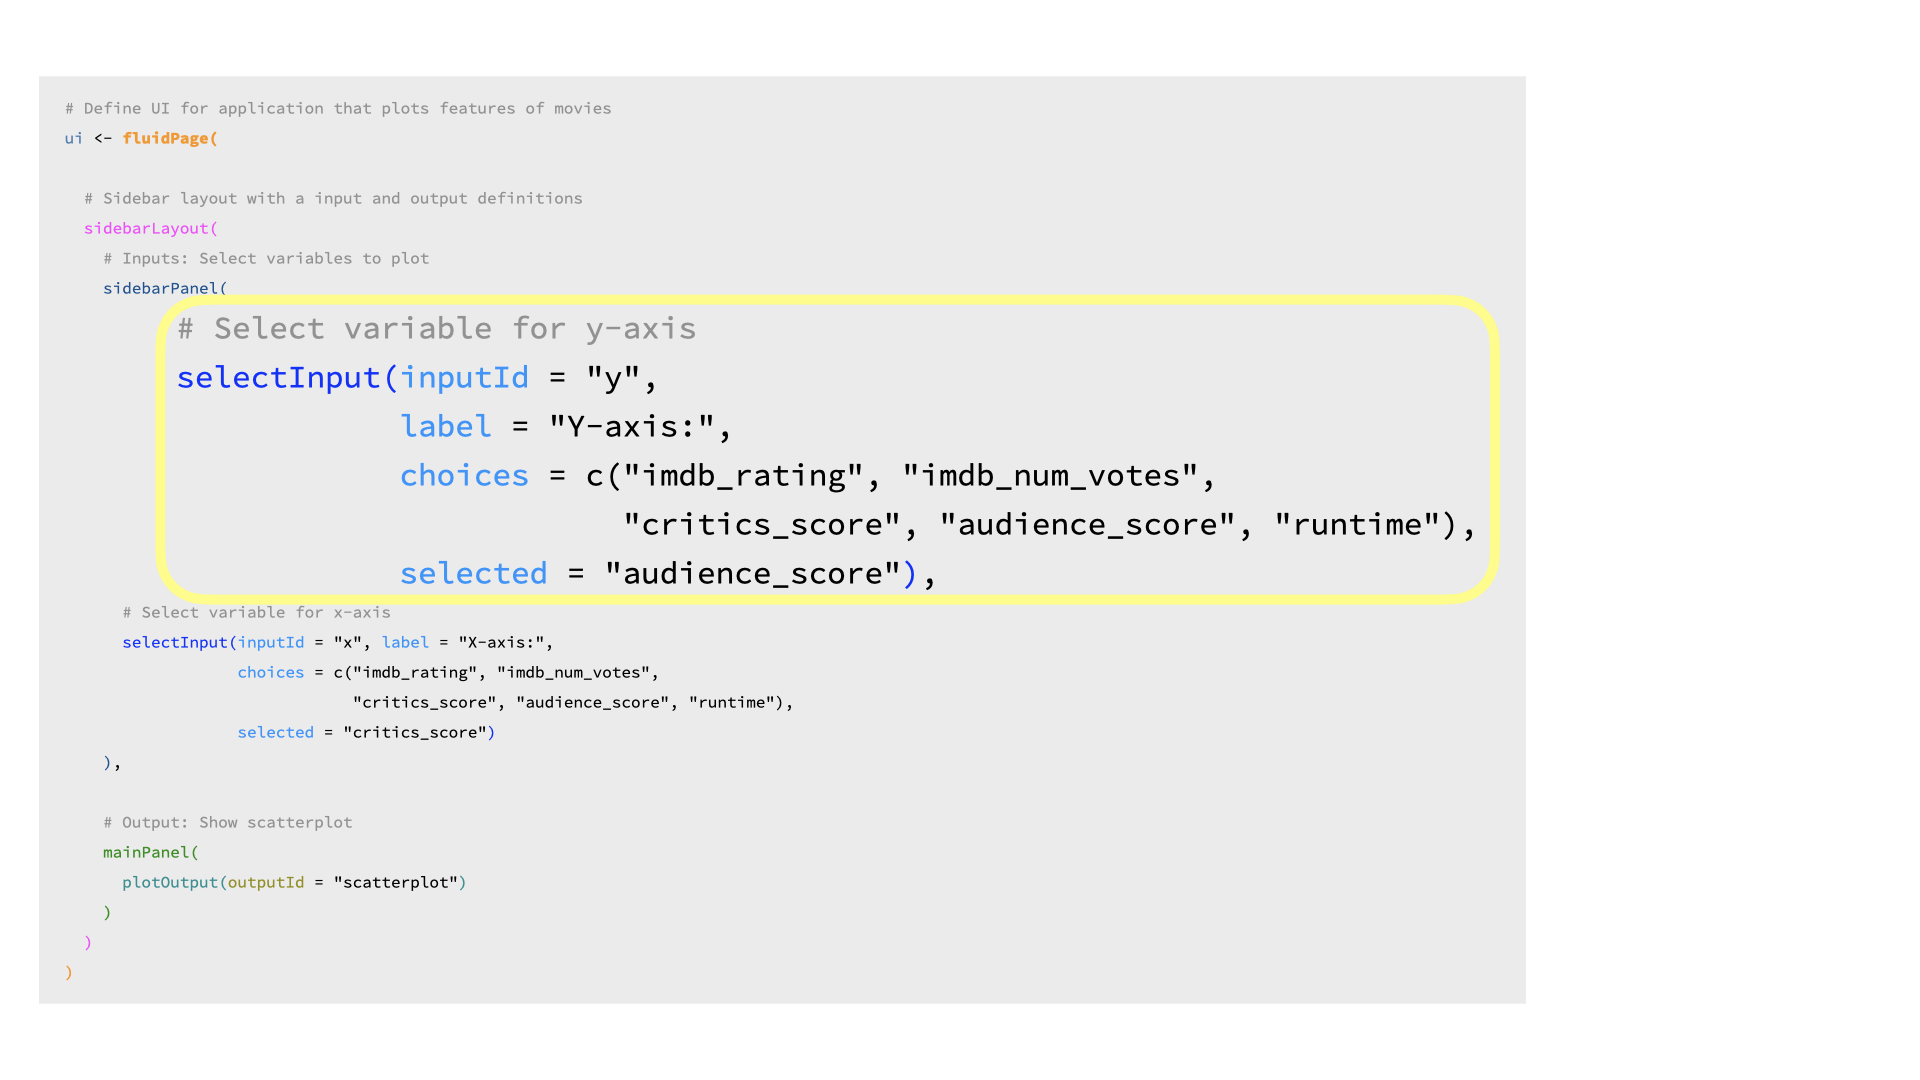
\includegraphics[width=1\textwidth,height=\textheight]{./images/input-closeup.png}

}

\end{figure}

\begin{enumerate}
\def\labelenumi{\arabic{enumi}.}
\item
  The first argument is the \texttt{inputId}, which is the input value
  that the app will internally use to access the value selected by the
  user.
\item
  The second argument is the \texttt{label}, which is the display label
  that the user sees.
\item
  The third argument is the list of \texttt{choices} the user will
  choose from. In this app, these are variable names from the movies
  dataset.
\item
  And lastly we specify a default selection from that list with
  \texttt{selected}.
\end{enumerate}

\hypertarget{main-panel-1}{%
\subsection{Main Panel}\label{main-panel-1}}

The final component of our UI is \texttt{mainPanel()}.

\begin{figure}

{\centering 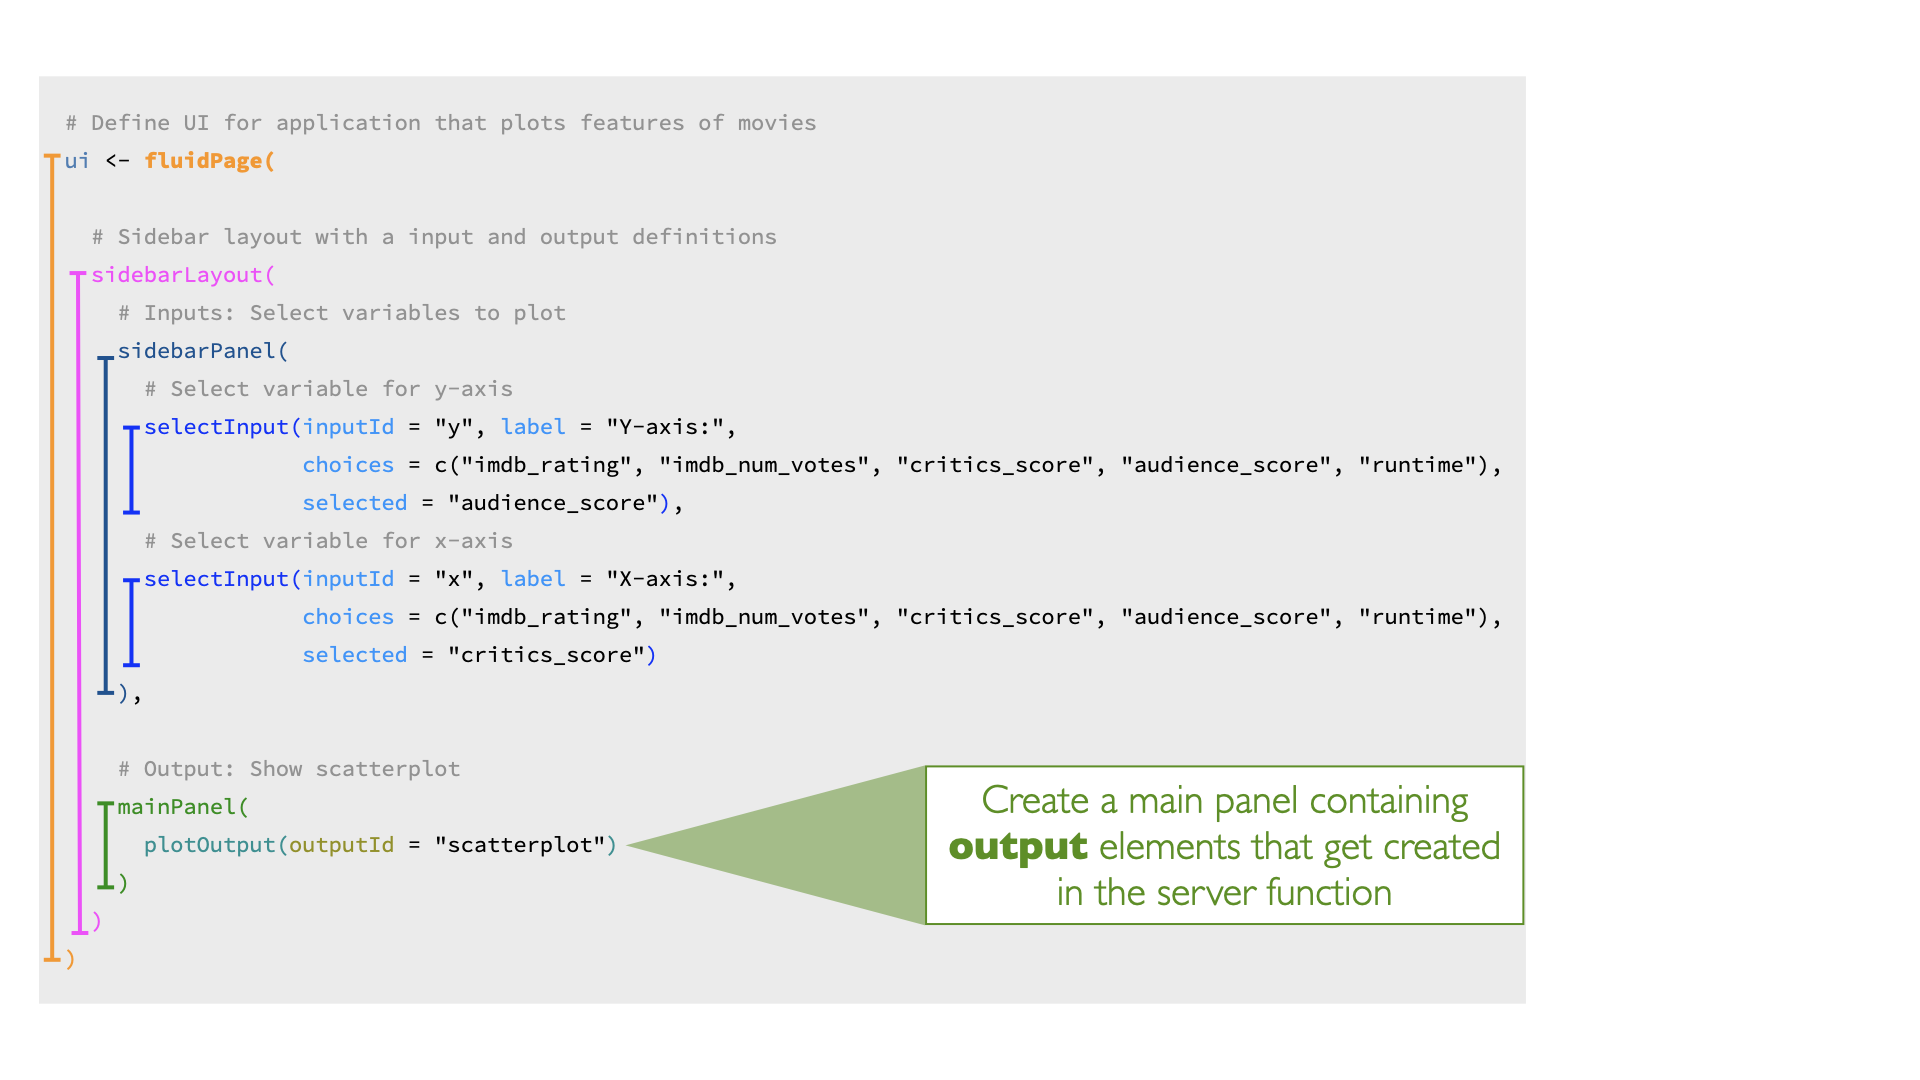
\includegraphics[width=1\textwidth,height=\textheight]{./images/main-panel.png}

}

\end{figure}

Currently the main panel contains only one component, a plot output.
We'll talk about how this plot is built later in the tutorial.

Next, let's practice building an app UI!

\hypertarget{practice-extend-the-ui-1}{%
\subsection{Practice: Extend the UI}\label{practice-extend-the-ui-1}}

We'll start with a simplified version of the app you saw in the previous
exercise. In this app a \texttt{selectInput()} widget is used to allow
the user to select which variables should be plotted on the \texttt{x}
and \texttt{y} axes of the scatterplot.

The \texttt{selectInput()} function has the following arguments:

\begin{itemize}
\tightlist
\item
  an \texttt{inputId} that is used to refer to the input parameter when
  building the scatterplot,
\item
  a list of \texttt{choices} to pick from (which must match variable
  names in the data frame),
\item
  and a \texttt{selected} choice for when the app first launches.
\end{itemize}

\hypertarget{your-turn-4}{%
\subsubsection{Your turn}\label{your-turn-4}}

Modify the Shiny app code in \texttt{app.R} / shown below:

\begin{itemize}
\tightlist
\item
  In the \texttt{ui}:

  \begin{itemize}
  \tightlist
  \item
    Add a new \texttt{selectInput} widget to color the points by a
    choice of the following variables: \texttt{"title\_type"},
    \texttt{"genre"}, \texttt{"mpaa\_rating"},
    \texttt{"critics\_rating"}, \texttt{"audience\_rating"}.
  \item
    Make the default selection \texttt{"mpaa\_rating"}.
  \item
    Use \texttt{"z"} as the \texttt{inputId}.
  \item
    \texttt{label} can be whatever you like.
  \end{itemize}
\item
  In the \texttt{server}:

  \begin{itemize}
  \tightlist
  \item
    Set the color argument in \texttt{ggplot()} aesthetic mappings to
    \texttt{input\$z}.
  \end{itemize}
\end{itemize}

\emph{Complete this exercise by opening up the RStudio Project titled
\textbf{1-2a Extend the UI} within your RStudio Cloud Workspace}

\href{https://rstudio.cloud/spaces/81721/join?access_code=I4VJaNsKfTqR3Td9hLP7E1nz8\%2FtMg6Xbw9Bgqumv}{
Go to RStudio Cloud Workspace}

\begin{Shaded}
\begin{Highlighting}[]
\CommentTok{\# Load packages {-}{-}{-}{-}{-}{-}{-}{-}{-}{-}{-}{-}{-}{-}{-}{-}{-}{-}{-}{-}{-}{-}{-}{-}{-}{-}{-}{-}{-}{-}{-}{-}{-}{-}{-}{-}{-}{-}{-}{-}{-}{-}{-}{-}{-}{-}{-}{-}{-}{-}{-}{-}{-}{-}{-}{-}{-}{-}{-}{-}{-}{-}{-}{-}}

\FunctionTok{library}\NormalTok{(shiny)}
\FunctionTok{library}\NormalTok{(ggplot2)}

\CommentTok{\# Load data {-}{-}{-}{-}{-}{-}{-}{-}{-}{-}{-}{-}{-}{-}{-}{-}{-}{-}{-}{-}{-}{-}{-}{-}{-}{-}{-}{-}{-}{-}{-}{-}{-}{-}{-}{-}{-}{-}{-}{-}{-}{-}{-}{-}{-}{-}{-}{-}{-}{-}{-}{-}{-}{-}{-}{-}{-}{-}{-}{-}{-}{-}{-}{-}{-}{-}{-}{-}}

\FunctionTok{load}\NormalTok{(}\StringTok{"movies.RData"}\NormalTok{)}

\CommentTok{\# Define UI {-}{-}{-}{-}{-}{-}{-}{-}{-}{-}{-}{-}{-}{-}{-}{-}{-}{-}{-}{-}{-}{-}{-}{-}{-}{-}{-}{-}{-}{-}{-}{-}{-}{-}{-}{-}{-}{-}{-}{-}{-}{-}{-}{-}{-}{-}{-}{-}{-}{-}{-}{-}{-}{-}{-}{-}{-}{-}{-}{-}{-}{-}{-}{-}{-}{-}{-}{-}}

\NormalTok{ui }\OtherTok{\textless{}{-}} \FunctionTok{fluidPage}\NormalTok{(}
  
  \FunctionTok{sidebarLayout}\NormalTok{(}
    
    \CommentTok{\# Inputs: Select variables to plot}
    \FunctionTok{sidebarPanel}\NormalTok{(}
      
      \CommentTok{\# Select variable for y{-}axis}
      \FunctionTok{selectInput}\NormalTok{(}\AttributeTok{inputId =} \StringTok{"y"}\NormalTok{, }
                  \AttributeTok{label =} \StringTok{"Y{-}axis:"}\NormalTok{,}
                  \AttributeTok{choices =} \FunctionTok{c}\NormalTok{(}\StringTok{"imdb\_rating"}\NormalTok{, }\StringTok{"imdb\_num\_votes"}\NormalTok{, }\StringTok{"critics\_score"}\NormalTok{, }\StringTok{"audience\_score"}\NormalTok{, }\StringTok{"runtime"}\NormalTok{), }
                  \AttributeTok{selected =} \StringTok{"audience\_score"}\NormalTok{),}
      
      \CommentTok{\# Select variable for x{-}axis}
      \FunctionTok{selectInput}\NormalTok{(}\AttributeTok{inputId =} \StringTok{"x"}\NormalTok{, }
                  \AttributeTok{label =} \StringTok{"X{-}axis:"}\NormalTok{,}
                  \AttributeTok{choices =} \FunctionTok{c}\NormalTok{(}\StringTok{"imdb\_rating"}\NormalTok{, }\StringTok{"imdb\_num\_votes"}\NormalTok{, }\StringTok{"critics\_score"}\NormalTok{, }\StringTok{"audience\_score"}\NormalTok{, }\StringTok{"runtime"}\NormalTok{), }
                  \AttributeTok{selected =} \StringTok{"critics\_score"}\NormalTok{),}
      
      \CommentTok{\# Select variable for color}
      \FunctionTok{selectInput}\NormalTok{(}\AttributeTok{inputId =} \StringTok{"\_\_\_"}\NormalTok{, }
                  \AttributeTok{label =} \StringTok{"\_\_\_\_"}\NormalTok{,}
                  \AttributeTok{choices =} \FunctionTok{c}\NormalTok{(\_\_\_),}
                  \AttributeTok{selected =} \StringTok{"\_\_\_"}\NormalTok{)}
      
\NormalTok{    ),}
    
    \CommentTok{\# Output: Show scatterplot}
    \FunctionTok{mainPanel}\NormalTok{(}
      \FunctionTok{plotOutput}\NormalTok{(}\AttributeTok{outputId =} \StringTok{"scatterplot"}\NormalTok{)}
\NormalTok{    )}
\NormalTok{  )}
\NormalTok{)}

\CommentTok{\# Define server {-}{-}{-}{-}{-}{-}{-}{-}{-}{-}{-}{-}{-}{-}{-}{-}{-}{-}{-}{-}{-}{-}{-}{-}{-}{-}{-}{-}{-}{-}{-}{-}{-}{-}{-}{-}{-}{-}{-}{-}{-}{-}{-}{-}{-}{-}{-}{-}{-}{-}{-}{-}{-}{-}{-}{-}{-}{-}{-}{-}{-}{-}{-}{-}}

\NormalTok{server }\OtherTok{\textless{}{-}} \ControlFlowTok{function}\NormalTok{(input, output, session) \{}
  
\NormalTok{  output}\SpecialCharTok{$}\NormalTok{scatterplot }\OtherTok{\textless{}{-}} \FunctionTok{renderPlot}\NormalTok{(\{}
    \FunctionTok{ggplot}\NormalTok{(}\AttributeTok{data =}\NormalTok{ movies, }\FunctionTok{aes\_string}\NormalTok{(}\AttributeTok{x =}\NormalTok{ input}\SpecialCharTok{$}\NormalTok{x, }\AttributeTok{y =}\NormalTok{ input}\SpecialCharTok{$}\NormalTok{y,}
                                     \AttributeTok{color =}\NormalTok{ \_\_\_)) }\SpecialCharTok{+}
      \FunctionTok{geom\_point}\NormalTok{()}
\NormalTok{  \})}
  
\NormalTok{  \}}

\CommentTok{\# Create a Shiny app object {-}{-}{-}{-}{-}{-}{-}{-}{-}{-}{-}{-}{-}{-}{-}{-}{-}{-}{-}{-}{-}{-}{-}{-}{-}{-}{-}{-}{-}{-}{-}{-}{-}{-}{-}{-}{-}{-}{-}{-}{-}{-}{-}{-}{-}{-}{-}{-}{-}{-}{-}{-}}

\FunctionTok{shinyApp}\NormalTok{(}\AttributeTok{ui =}\NormalTok{ ui, }\AttributeTok{server =}\NormalTok{ server)}
\end{Highlighting}
\end{Shaded}

Show solution

See the following code chunk for the solution to the exercise above.

\begin{Shaded}
\begin{Highlighting}[]
\CommentTok{\# Load packages {-}{-}{-}{-}{-}{-}{-}{-}{-}{-}{-}{-}{-}{-}{-}{-}{-}{-}{-}{-}{-}{-}{-}{-}{-}{-}{-}{-}{-}{-}{-}{-}{-}{-}{-}{-}{-}{-}{-}{-}{-}{-}{-}{-}{-}{-}{-}{-}{-}{-}{-}{-}{-}{-}{-}{-}{-}{-}{-}{-}{-}{-}{-}{-}}

\FunctionTok{library}\NormalTok{(shiny)}
\FunctionTok{library}\NormalTok{(ggplot2)}

\CommentTok{\# Load data {-}{-}{-}{-}{-}{-}{-}{-}{-}{-}{-}{-}{-}{-}{-}{-}{-}{-}{-}{-}{-}{-}{-}{-}{-}{-}{-}{-}{-}{-}{-}{-}{-}{-}{-}{-}{-}{-}{-}{-}{-}{-}{-}{-}{-}{-}{-}{-}{-}{-}{-}{-}{-}{-}{-}{-}{-}{-}{-}{-}{-}{-}{-}{-}{-}{-}{-}{-}}

\FunctionTok{load}\NormalTok{(}\StringTok{"movies.RData"}\NormalTok{)}

\CommentTok{\# Define UI {-}{-}{-}{-}{-}{-}{-}{-}{-}{-}{-}{-}{-}{-}{-}{-}{-}{-}{-}{-}{-}{-}{-}{-}{-}{-}{-}{-}{-}{-}{-}{-}{-}{-}{-}{-}{-}{-}{-}{-}{-}{-}{-}{-}{-}{-}{-}{-}{-}{-}{-}{-}{-}{-}{-}{-}{-}{-}{-}{-}{-}{-}{-}{-}{-}{-}{-}{-}}

\NormalTok{ui }\OtherTok{\textless{}{-}} \FunctionTok{fluidPage}\NormalTok{(}
  
  \FunctionTok{sidebarLayout}\NormalTok{(}
    
    \CommentTok{\# Inputs: Select variables to plot}
    \FunctionTok{sidebarPanel}\NormalTok{(}
      
      \CommentTok{\# Select variable for y{-}axis}
      \FunctionTok{selectInput}\NormalTok{(}\AttributeTok{inputId =} \StringTok{"y"}\NormalTok{, }
                  \AttributeTok{label =} \StringTok{"Y{-}axis:"}\NormalTok{,}
                  \AttributeTok{choices =} \FunctionTok{c}\NormalTok{(}\StringTok{"imdb\_rating"}\NormalTok{, }\StringTok{"imdb\_num\_votes"}\NormalTok{, }\StringTok{"critics\_score"}\NormalTok{, }\StringTok{"audience\_score"}\NormalTok{, }\StringTok{"runtime"}\NormalTok{), }
                  \AttributeTok{selected =} \StringTok{"audience\_score"}\NormalTok{),}
      
      \CommentTok{\# Select variable for x{-}axis}
      \FunctionTok{selectInput}\NormalTok{(}\AttributeTok{inputId =} \StringTok{"x"}\NormalTok{, }
                  \AttributeTok{label =} \StringTok{"X{-}axis:"}\NormalTok{,}
                  \AttributeTok{choices =} \FunctionTok{c}\NormalTok{(}\StringTok{"imdb\_rating"}\NormalTok{, }\StringTok{"imdb\_num\_votes"}\NormalTok{, }\StringTok{"critics\_score"}\NormalTok{, }\StringTok{"audience\_score"}\NormalTok{, }\StringTok{"runtime"}\NormalTok{), }
                  \AttributeTok{selected =} \StringTok{"critics\_score"}\NormalTok{),}
      
      \CommentTok{\# Select variable for color}
      \FunctionTok{selectInput}\NormalTok{(}\AttributeTok{inputId =} \StringTok{"z"}\NormalTok{, }
                  \AttributeTok{label =} \StringTok{"Color by:"}\NormalTok{,}
                  \AttributeTok{choices =} \FunctionTok{c}\NormalTok{(}\StringTok{"title\_type"}\NormalTok{, }\StringTok{"genre"}\NormalTok{, }\StringTok{"mpaa\_rating"}\NormalTok{, }\StringTok{"critics\_rating"}\NormalTok{, }\StringTok{"audience\_rating"}\NormalTok{),}
                  \AttributeTok{selected =} \StringTok{"mpaa\_rating"}\NormalTok{)}
      
\NormalTok{    ),}
    
    \CommentTok{\# Output: Show scatterplot}
    \FunctionTok{mainPanel}\NormalTok{(}
      \FunctionTok{plotOutput}\NormalTok{(}\AttributeTok{outputId =} \StringTok{"scatterplot"}\NormalTok{)}
\NormalTok{    )}
\NormalTok{  )}
\NormalTok{)}

\CommentTok{\# Define server {-}{-}{-}{-}{-}{-}{-}{-}{-}{-}{-}{-}{-}{-}{-}{-}{-}{-}{-}{-}{-}{-}{-}{-}{-}{-}{-}{-}{-}{-}{-}{-}{-}{-}{-}{-}{-}{-}{-}{-}{-}{-}{-}{-}{-}{-}{-}{-}{-}{-}{-}{-}{-}{-}{-}{-}{-}{-}{-}{-}{-}{-}{-}{-}}

\NormalTok{server }\OtherTok{\textless{}{-}} \ControlFlowTok{function}\NormalTok{(input, output, session) \{}
  
\NormalTok{  output}\SpecialCharTok{$}\NormalTok{scatterplot }\OtherTok{\textless{}{-}} \FunctionTok{renderPlot}\NormalTok{(\{}
    \FunctionTok{ggplot}\NormalTok{(}\AttributeTok{data =}\NormalTok{ movies, }\FunctionTok{aes\_string}\NormalTok{(}\AttributeTok{x =}\NormalTok{ input}\SpecialCharTok{$}\NormalTok{x, }\AttributeTok{y =}\NormalTok{ input}\SpecialCharTok{$}\NormalTok{y,}
                                     \AttributeTok{color =}\NormalTok{ input}\SpecialCharTok{$}\NormalTok{z)) }\SpecialCharTok{+}
      \FunctionTok{geom\_point}\NormalTok{()}
\NormalTok{  \})}
  
\NormalTok{  \}}

\CommentTok{\# Create a Shiny app object {-}{-}{-}{-}{-}{-}{-}{-}{-}{-}{-}{-}{-}{-}{-}{-}{-}{-}{-}{-}{-}{-}{-}{-}{-}{-}{-}{-}{-}{-}{-}{-}{-}{-}{-}{-}{-}{-}{-}{-}{-}{-}{-}{-}{-}{-}{-}{-}{-}{-}{-}{-}}

\FunctionTok{shinyApp}\NormalTok{(}\AttributeTok{ui =}\NormalTok{ ui, }\AttributeTok{server =}\NormalTok{ server)}
\end{Highlighting}
\end{Shaded}

\hypertarget{practice-extend-the-ui-further-1}{%
\subsection{Practice: Extend the UI
further}\label{practice-extend-the-ui-further-1}}

The potential variables the user can select for the \texttt{x} and
\texttt{y} axes and \texttt{color} currently appear in the UI of the app
the same way that they are spelled in the data frame header. However we
might want to label them in a way that is more human readable. We can
achieve this using named vectors for the \texttt{choices} argument, in
the format of \texttt{"Human\ readable\ label"\ =\ "variable\_name"}.

\hypertarget{your-turn-5}{%
\subsubsection{Your turn}\label{your-turn-5}}

\begin{itemize}
\tightlist
\item
  Fill in the blanks in the code below with human readable labels for
  \texttt{x} and \texttt{y} inputs.
\item
  Re-create the \texttt{selectInput} widget for color, \texttt{z}, with
  options \texttt{"title\_type"}, \texttt{"genre"},
  \texttt{"mpaa\_rating"}, \texttt{"critics\_rating"}, and
  \texttt{"audience\_rating"}, default selection \texttt{"mpaa\_rating"}
  just like in the previous exercise, but this time use human readable
  labels as well.
\end{itemize}

\emph{Complete this exercise by opening up the RStudio Project titled
\textbf{1-2b Extend the UI further} within your RStudio Cloud Workspace}

\href{https://rstudio.cloud/spaces/81721/join?access_code=I4VJaNsKfTqR3Td9hLP7E1nz8\%2FtMg6Xbw9Bgqumv}{
Go to RStudio Cloud Workspace}

\begin{Shaded}
\begin{Highlighting}[]
\CommentTok{\# Load packages {-}{-}{-}{-}{-}{-}{-}{-}{-}{-}{-}{-}{-}{-}{-}{-}{-}{-}{-}{-}{-}{-}{-}{-}{-}{-}{-}{-}{-}{-}{-}{-}{-}{-}{-}{-}{-}{-}{-}{-}{-}{-}{-}{-}{-}{-}{-}{-}{-}{-}{-}{-}{-}{-}{-}{-}{-}{-}{-}{-}{-}{-}{-}{-}}

\FunctionTok{library}\NormalTok{(shiny)}
\FunctionTok{library}\NormalTok{(ggplot2)}

\CommentTok{\# Load data {-}{-}{-}{-}{-}{-}{-}{-}{-}{-}{-}{-}{-}{-}{-}{-}{-}{-}{-}{-}{-}{-}{-}{-}{-}{-}{-}{-}{-}{-}{-}{-}{-}{-}{-}{-}{-}{-}{-}{-}{-}{-}{-}{-}{-}{-}{-}{-}{-}{-}{-}{-}{-}{-}{-}{-}{-}{-}{-}{-}{-}{-}{-}{-}{-}{-}{-}{-}}

\FunctionTok{load}\NormalTok{(}\StringTok{"movies.RData"}\NormalTok{)}

\CommentTok{\# Define UI {-}{-}{-}{-}{-}{-}{-}{-}{-}{-}{-}{-}{-}{-}{-}{-}{-}{-}{-}{-}{-}{-}{-}{-}{-}{-}{-}{-}{-}{-}{-}{-}{-}{-}{-}{-}{-}{-}{-}{-}{-}{-}{-}{-}{-}{-}{-}{-}{-}{-}{-}{-}{-}{-}{-}{-}{-}{-}{-}{-}{-}{-}{-}{-}{-}{-}{-}{-}}

\NormalTok{ui }\OtherTok{\textless{}{-}} \FunctionTok{fluidPage}\NormalTok{(}
  
  \FunctionTok{sidebarLayout}\NormalTok{(}
    
    \CommentTok{\# Inputs: Select variables to plot}
    \FunctionTok{sidebarPanel}\NormalTok{(}
      
      \CommentTok{\# Select variable for y{-}axis}
      \FunctionTok{selectInput}\NormalTok{(}\AttributeTok{inputId =} \StringTok{"y"}\NormalTok{, }
                  \AttributeTok{label =} \StringTok{"Y{-}axis:"}\NormalTok{,}
                  \AttributeTok{choices =} \FunctionTok{c}\NormalTok{(}\AttributeTok{\_\_\_ =} \StringTok{"imdb\_rating"}\NormalTok{, }
                              \AttributeTok{\_\_\_ =} \StringTok{"imdb\_num\_votes"}\NormalTok{, }
                              \AttributeTok{\_\_\_ =} \StringTok{"critics\_score"}\NormalTok{, }
                              \AttributeTok{\_\_\_ =} \StringTok{"audience\_score"}\NormalTok{, }
                              \AttributeTok{\_\_\_ =} \StringTok{"runtime"}\NormalTok{), }
                  \AttributeTok{selected =} \StringTok{"audience\_score"}\NormalTok{),}
      
      \CommentTok{\# Select variable for x{-}axis}
      \FunctionTok{selectInput}\NormalTok{(}\AttributeTok{inputId =} \StringTok{"x"}\NormalTok{, }
                  \AttributeTok{label =} \StringTok{"X{-}axis:"}\NormalTok{,}
                  \AttributeTok{choices =} \FunctionTok{c}\NormalTok{(}\AttributeTok{\_\_\_ =} \StringTok{"imdb\_rating"}\NormalTok{, }
                              \AttributeTok{\_\_\_ =} \StringTok{"imdb\_num\_votes"}\NormalTok{, }
                              \AttributeTok{\_\_\_ =} \StringTok{"critics\_score"}\NormalTok{, }
                              \AttributeTok{\_\_\_ =} \StringTok{"audience\_score"}\NormalTok{, }
                              \AttributeTok{\_\_\_ =} \StringTok{"runtime"}\NormalTok{), }
                  \AttributeTok{selected =} \StringTok{"critics\_score"}\NormalTok{),}
      
      \CommentTok{\# Select variable for color}
      \FunctionTok{selectInput}\NormalTok{(}\AttributeTok{inputId =} \StringTok{"z"}\NormalTok{, }
                  \AttributeTok{label =} \StringTok{"Color:"}\NormalTok{,}
                  \AttributeTok{choices =}\NormalTok{ \_\_\_, }
                  \AttributeTok{selected =}\NormalTok{ \_\_\_)}
      
\NormalTok{    ),}
    
    \CommentTok{\# Output: Show scatterplot}
    \FunctionTok{mainPanel}\NormalTok{(}
      \FunctionTok{plotOutput}\NormalTok{(}\AttributeTok{outputId =} \StringTok{"scatterplot"}\NormalTok{)}
\NormalTok{    )}
\NormalTok{  )}
\NormalTok{)}

\CommentTok{\# Define server {-}{-}{-}{-}{-}{-}{-}{-}{-}{-}{-}{-}{-}{-}{-}{-}{-}{-}{-}{-}{-}{-}{-}{-}{-}{-}{-}{-}{-}{-}{-}{-}{-}{-}{-}{-}{-}{-}{-}{-}{-}{-}{-}{-}{-}{-}{-}{-}{-}{-}{-}{-}{-}{-}{-}{-}{-}{-}{-}{-}{-}{-}{-}{-}}

\NormalTok{server }\OtherTok{\textless{}{-}} \ControlFlowTok{function}\NormalTok{(input, output, session) \{}
  
\NormalTok{  output}\SpecialCharTok{$}\NormalTok{scatterplot }\OtherTok{\textless{}{-}} \FunctionTok{renderPlot}\NormalTok{(\{}
    \FunctionTok{ggplot}\NormalTok{(}\AttributeTok{data =}\NormalTok{ movies, }\FunctionTok{aes\_string}\NormalTok{(}\AttributeTok{x =}\NormalTok{ input}\SpecialCharTok{$}\NormalTok{x, }\AttributeTok{y =}\NormalTok{ input}\SpecialCharTok{$}\NormalTok{y,}
                                     \AttributeTok{color =}\NormalTok{ input}\SpecialCharTok{$}\NormalTok{z)) }\SpecialCharTok{+}
      \FunctionTok{geom\_point}\NormalTok{()}
\NormalTok{  \})}
  
\NormalTok{  \}}

\CommentTok{\# Create a Shiny app object {-}{-}{-}{-}{-}{-}{-}{-}{-}{-}{-}{-}{-}{-}{-}{-}{-}{-}{-}{-}{-}{-}{-}{-}{-}{-}{-}{-}{-}{-}{-}{-}{-}{-}{-}{-}{-}{-}{-}{-}{-}{-}{-}{-}{-}{-}{-}{-}{-}{-}{-}{-}}

\FunctionTok{shinyApp}\NormalTok{(}\AttributeTok{ui =}\NormalTok{ ui, }\AttributeTok{server =}\NormalTok{ server)}
\end{Highlighting}
\end{Shaded}

Show solution

See the following code chunk for the solution to the exercise above.

\begin{Shaded}
\begin{Highlighting}[]
\CommentTok{\# Load packages {-}{-}{-}{-}{-}{-}{-}{-}{-}{-}{-}{-}{-}{-}{-}{-}{-}{-}{-}{-}{-}{-}{-}{-}{-}{-}{-}{-}{-}{-}{-}{-}{-}{-}{-}{-}{-}{-}{-}{-}{-}{-}{-}{-}{-}{-}{-}{-}{-}{-}{-}{-}{-}{-}{-}{-}{-}{-}{-}{-}{-}{-}{-}{-}}

\FunctionTok{library}\NormalTok{(shiny)}
\FunctionTok{library}\NormalTok{(ggplot2)}

\CommentTok{\# Load data {-}{-}{-}{-}{-}{-}{-}{-}{-}{-}{-}{-}{-}{-}{-}{-}{-}{-}{-}{-}{-}{-}{-}{-}{-}{-}{-}{-}{-}{-}{-}{-}{-}{-}{-}{-}{-}{-}{-}{-}{-}{-}{-}{-}{-}{-}{-}{-}{-}{-}{-}{-}{-}{-}{-}{-}{-}{-}{-}{-}{-}{-}{-}{-}{-}{-}{-}{-}}

\FunctionTok{load}\NormalTok{(}\StringTok{"movies.RData"}\NormalTok{)}

\CommentTok{\# Define UI {-}{-}{-}{-}{-}{-}{-}{-}{-}{-}{-}{-}{-}{-}{-}{-}{-}{-}{-}{-}{-}{-}{-}{-}{-}{-}{-}{-}{-}{-}{-}{-}{-}{-}{-}{-}{-}{-}{-}{-}{-}{-}{-}{-}{-}{-}{-}{-}{-}{-}{-}{-}{-}{-}{-}{-}{-}{-}{-}{-}{-}{-}{-}{-}{-}{-}{-}{-}}

\NormalTok{ui }\OtherTok{\textless{}{-}} \FunctionTok{fluidPage}\NormalTok{(}
  
  \FunctionTok{sidebarLayout}\NormalTok{(}
    
    \CommentTok{\# Inputs: Select variables to plot}
    \FunctionTok{sidebarPanel}\NormalTok{(}
      
      \CommentTok{\# Select variable for y{-}axis}
      \FunctionTok{selectInput}\NormalTok{(}\AttributeTok{inputId =} \StringTok{"y"}\NormalTok{, }
                  \AttributeTok{label =} \StringTok{"Y{-}axis:"}\NormalTok{,}
                  \AttributeTok{choices =} \FunctionTok{c}\NormalTok{(}\StringTok{"IMDB rating"}          \OtherTok{=} \StringTok{"imdb\_rating"}\NormalTok{, }
                              \StringTok{"IMDB number of votes"} \OtherTok{=} \StringTok{"imdb\_num\_votes"}\NormalTok{, }
                              \StringTok{"Critics score"}        \OtherTok{=} \StringTok{"critics\_score"}\NormalTok{, }
                              \StringTok{"Audience score"}       \OtherTok{=} \StringTok{"audience\_score"}\NormalTok{, }
                              \StringTok{"Runtime"}              \OtherTok{=} \StringTok{"runtime"}\NormalTok{), }
                  \AttributeTok{selected =} \StringTok{"audience\_score"}\NormalTok{),}
      
      \CommentTok{\# Select variable for x{-}axis}
      \FunctionTok{selectInput}\NormalTok{(}\AttributeTok{inputId =} \StringTok{"x"}\NormalTok{, }
                  \AttributeTok{label =} \StringTok{"X{-}axis:"}\NormalTok{,}
                  \AttributeTok{choices =} \FunctionTok{c}\NormalTok{(}
                    \StringTok{"IMDB rating"}          \OtherTok{=} \StringTok{"imdb\_rating"}\NormalTok{, }
                    \StringTok{"IMDB number of votes"} \OtherTok{=} \StringTok{"imdb\_num\_votes"}\NormalTok{, }
                    \StringTok{"Critics score"}        \OtherTok{=} \StringTok{"critics\_score"}\NormalTok{, }
                    \StringTok{"Audience score"}       \OtherTok{=} \StringTok{"audience\_score"}\NormalTok{, }
                    \StringTok{"Runtime"}              \OtherTok{=} \StringTok{"runtime"}\NormalTok{), }
                  \AttributeTok{selected =} \StringTok{"critics\_score"}\NormalTok{),}
      
      \CommentTok{\# Select variable for color}
      \CommentTok{\# Select variable for color}
      \FunctionTok{selectInput}\NormalTok{(}\AttributeTok{inputId =} \StringTok{"z"}\NormalTok{, }
                  \AttributeTok{label =} \StringTok{"Color by:"}\NormalTok{,}
                  \AttributeTok{choices =} \FunctionTok{c}\NormalTok{(}
                    \StringTok{"Title type"} \OtherTok{=} \StringTok{"title\_type"}\NormalTok{, }
                    \StringTok{"Genre"} \OtherTok{=} \StringTok{"genre"}\NormalTok{, }
                    \StringTok{"MPAA rating"} \OtherTok{=} \StringTok{"mpaa\_rating"}\NormalTok{, }
                    \StringTok{"Critics rating"} \OtherTok{=} \StringTok{"critics\_rating"}\NormalTok{, }
                    \StringTok{"Audience rating"} \OtherTok{=} \StringTok{"audience\_rating"}\NormalTok{),}
                  \AttributeTok{selected =} \StringTok{"mpaa\_rating"}\NormalTok{)}
      
\NormalTok{    ),}
    
    \CommentTok{\# Output: Show scatterplot}
    \FunctionTok{mainPanel}\NormalTok{(}
      \FunctionTok{plotOutput}\NormalTok{(}\AttributeTok{outputId =} \StringTok{"scatterplot"}\NormalTok{)}
\NormalTok{    )}
\NormalTok{  )}
\NormalTok{)}

\CommentTok{\# Define server {-}{-}{-}{-}{-}{-}{-}{-}{-}{-}{-}{-}{-}{-}{-}{-}{-}{-}{-}{-}{-}{-}{-}{-}{-}{-}{-}{-}{-}{-}{-}{-}{-}{-}{-}{-}{-}{-}{-}{-}{-}{-}{-}{-}{-}{-}{-}{-}{-}{-}{-}{-}{-}{-}{-}{-}{-}{-}{-}{-}{-}{-}{-}{-}}

\NormalTok{server }\OtherTok{\textless{}{-}} \ControlFlowTok{function}\NormalTok{(input, output, session) \{}
  
\NormalTok{  output}\SpecialCharTok{$}\NormalTok{scatterplot }\OtherTok{\textless{}{-}} \FunctionTok{renderPlot}\NormalTok{(\{}
    \FunctionTok{ggplot}\NormalTok{(}\AttributeTok{data =}\NormalTok{ movies, }\FunctionTok{aes\_string}\NormalTok{(}\AttributeTok{x =}\NormalTok{ input}\SpecialCharTok{$}\NormalTok{x, }\AttributeTok{y =}\NormalTok{ input}\SpecialCharTok{$}\NormalTok{y,}
                                     \AttributeTok{color =}\NormalTok{ input}\SpecialCharTok{$}\NormalTok{z)) }\SpecialCharTok{+}
      \FunctionTok{geom\_point}\NormalTok{()}
\NormalTok{  \})}
  
\NormalTok{  \}}

\CommentTok{\# Create a Shiny app object {-}{-}{-}{-}{-}{-}{-}{-}{-}{-}{-}{-}{-}{-}{-}{-}{-}{-}{-}{-}{-}{-}{-}{-}{-}{-}{-}{-}{-}{-}{-}{-}{-}{-}{-}{-}{-}{-}{-}{-}{-}{-}{-}{-}{-}{-}{-}{-}{-}{-}{-}{-}}

\FunctionTok{shinyApp}\NormalTok{(}\AttributeTok{ui =}\NormalTok{ ui, }\AttributeTok{server =}\NormalTok{ server)}
\end{Highlighting}
\end{Shaded}

\hypertarget{server-function-1}{%
\section{Server function}\label{server-function-1}}

Now that you've had some practice with the UI, it's time to move on to
the server function.

Again, before we get into the details, let's remind ourselves of the
anatomy of a Shiny app. The basic task of the server function is to
define the relationship between inputs and outputs.

\hypertarget{here-again-is-the-app-that-we-are-working-with-in-this-module-1}{%
\subsection{Here again is the app that we are working with in this
module}\label{here-again-is-the-app-that-we-are-working-with-in-this-module-1}}

Earlier we saw how to build the UI of this app, and we also noted that
each input was tagged with an \texttt{inputId} that can be used to refer
to them in the server.

\begin{figure}

{\centering 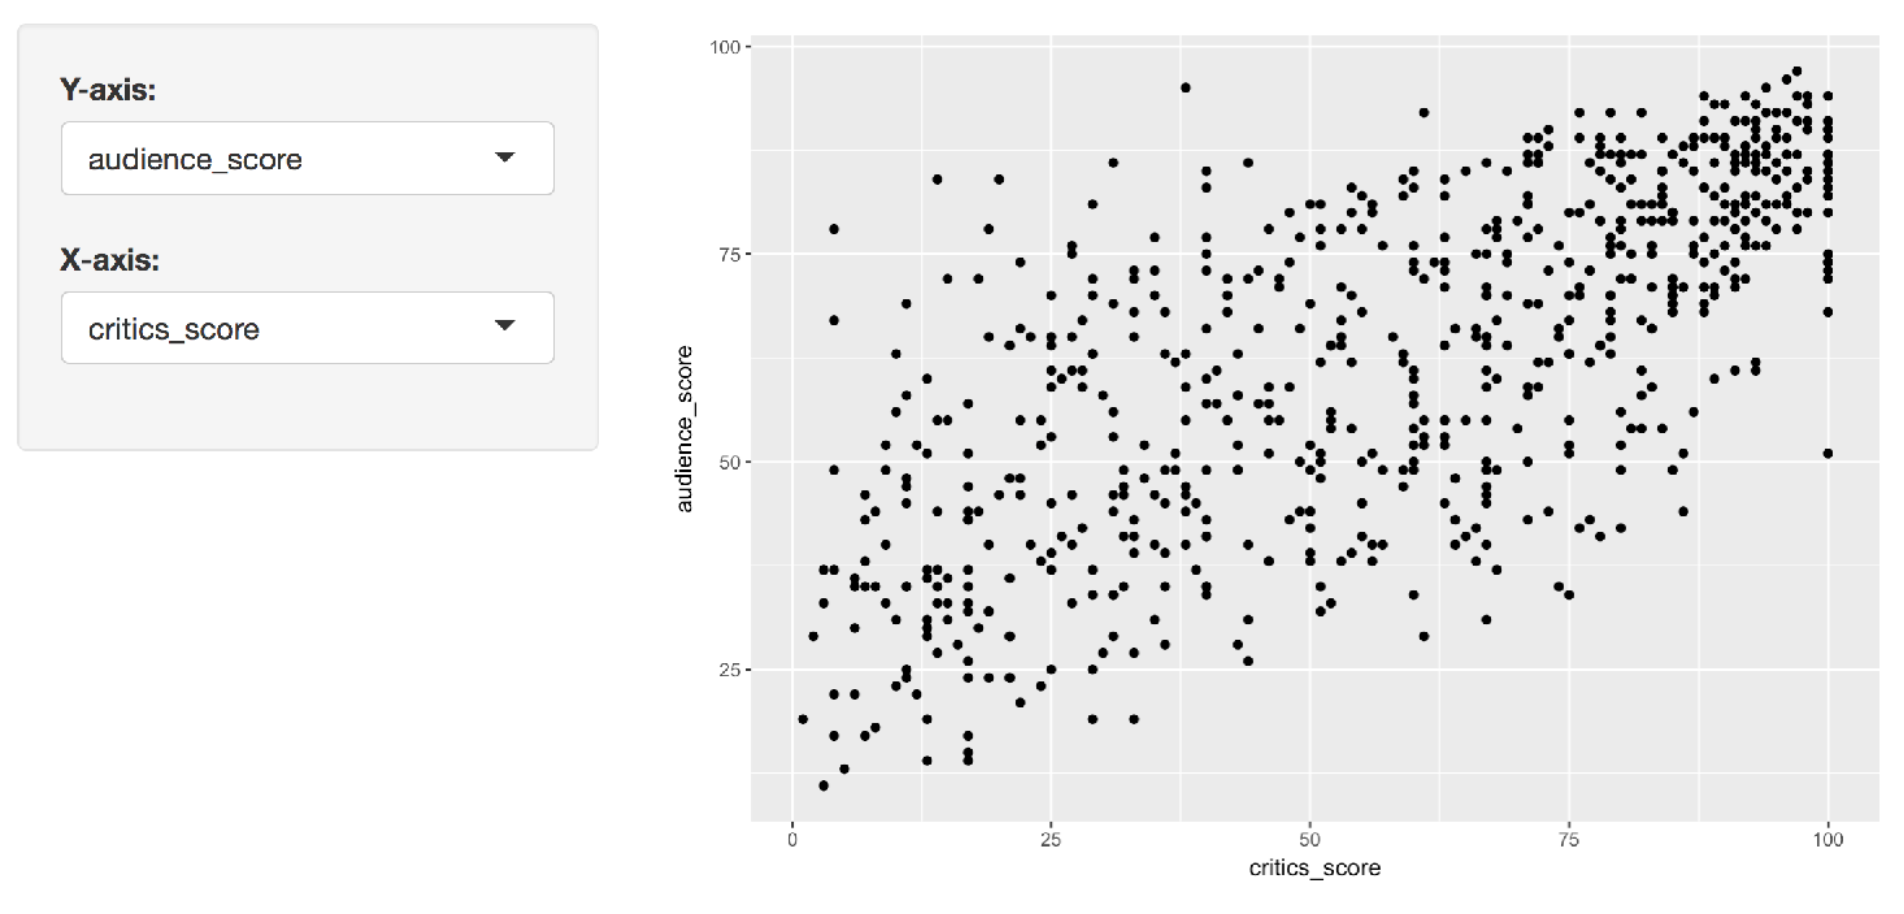
\includegraphics[width=1\textwidth,height=\textheight]{./images/app-selectinput-scatterplot.png}

}

\end{figure}

\hypertarget{this-is-the-server-function-code-for-this-app-1}{%
\subsection{This is the server function code for this
app}\label{this-is-the-server-function-code-for-this-app-1}}

Once again there is a lot going on here to parse at once, so in the
following sections we take a closer look at the function.

\begin{figure}

{\centering 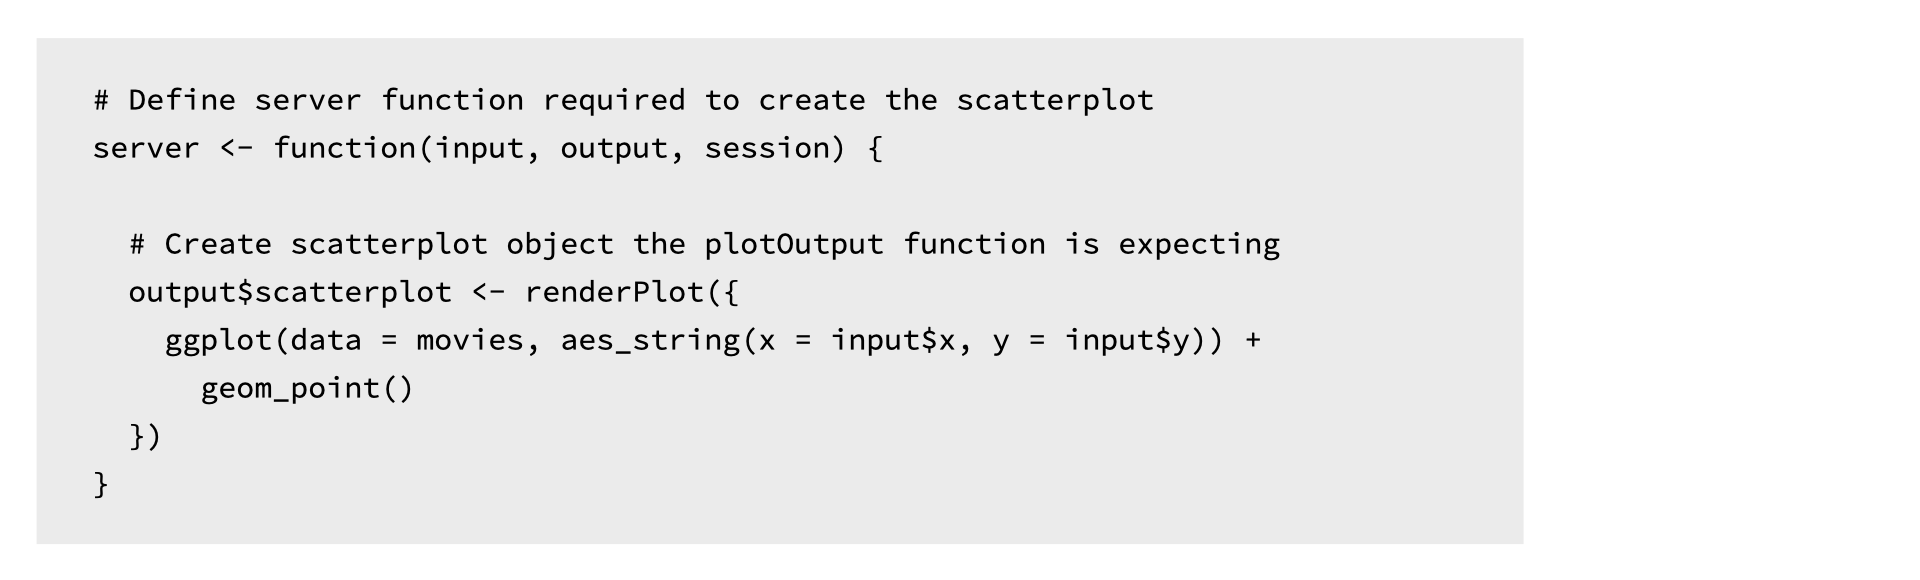
\includegraphics[width=1\textwidth,height=\textheight]{./images/server.png}

}

\end{figure}

\hypertarget{at-the-outermost-layer-1}{%
\subsection{At the outermost layer}\label{at-the-outermost-layer-1}}

\begin{figure}

{\centering 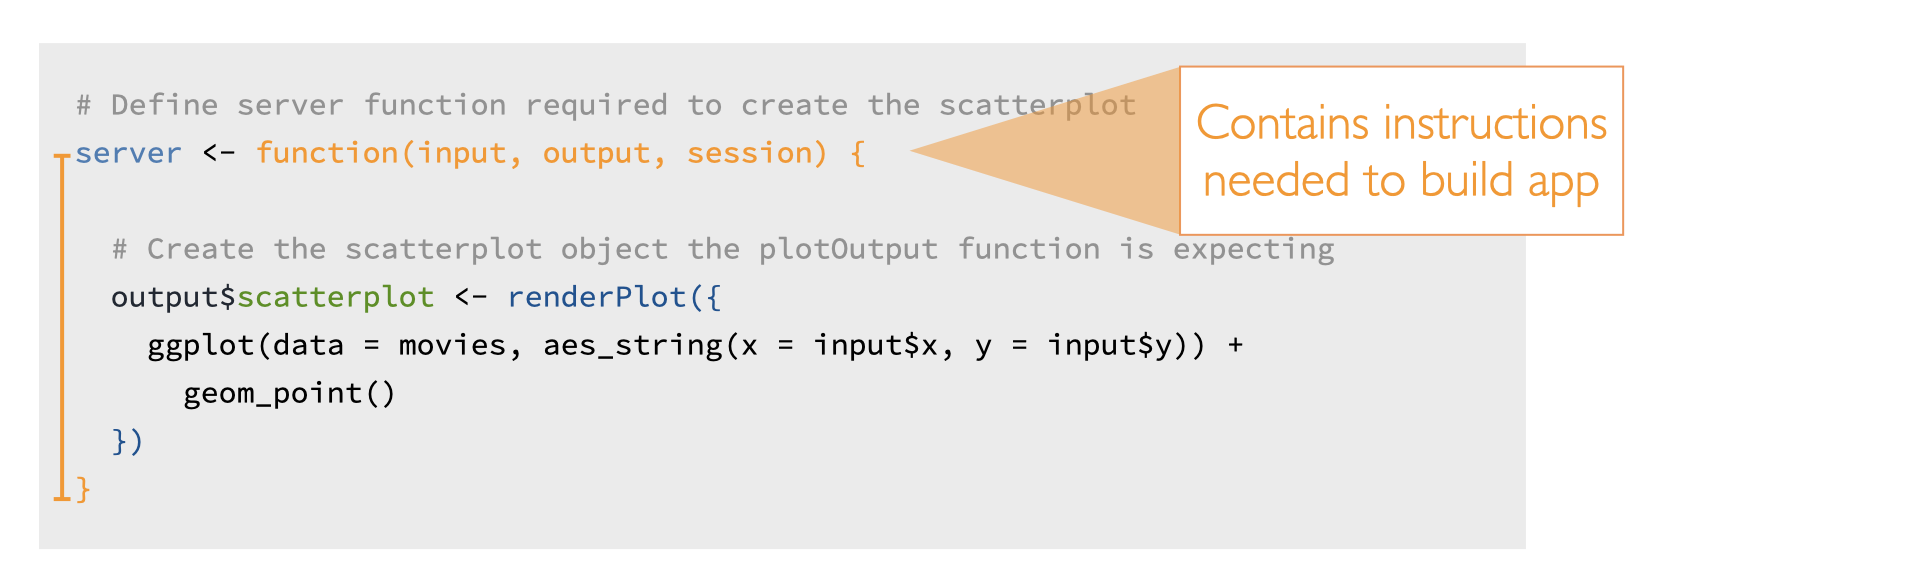
\includegraphics[width=1\textwidth,height=\textheight]{./images/server-outermost.png}

}

\end{figure}

We define our server function which takes two arguments: an
\texttt{input} and an \texttt{output}. Both of these are named lists.

The server function accesses inputs selected by the user to perform
computations and specifies how outputs laid out in the UI should be
updated.

The server function can take on one more argument, \texttt{session},
which is an environment that can be used to access information and
functionality relating to the session. However this concept is beyond
the scope of this tutorial, so for now we'll stick to server functions
that only have input and output arguments.

\hypertarget{output-1}{%
\subsection{\texorpdfstring{\texttt{output}}{output}}\label{output-1}}

Our simple app had only one output -- a plot. So our server function
contains the logic necessary to build this plot.

\begin{figure}

{\centering 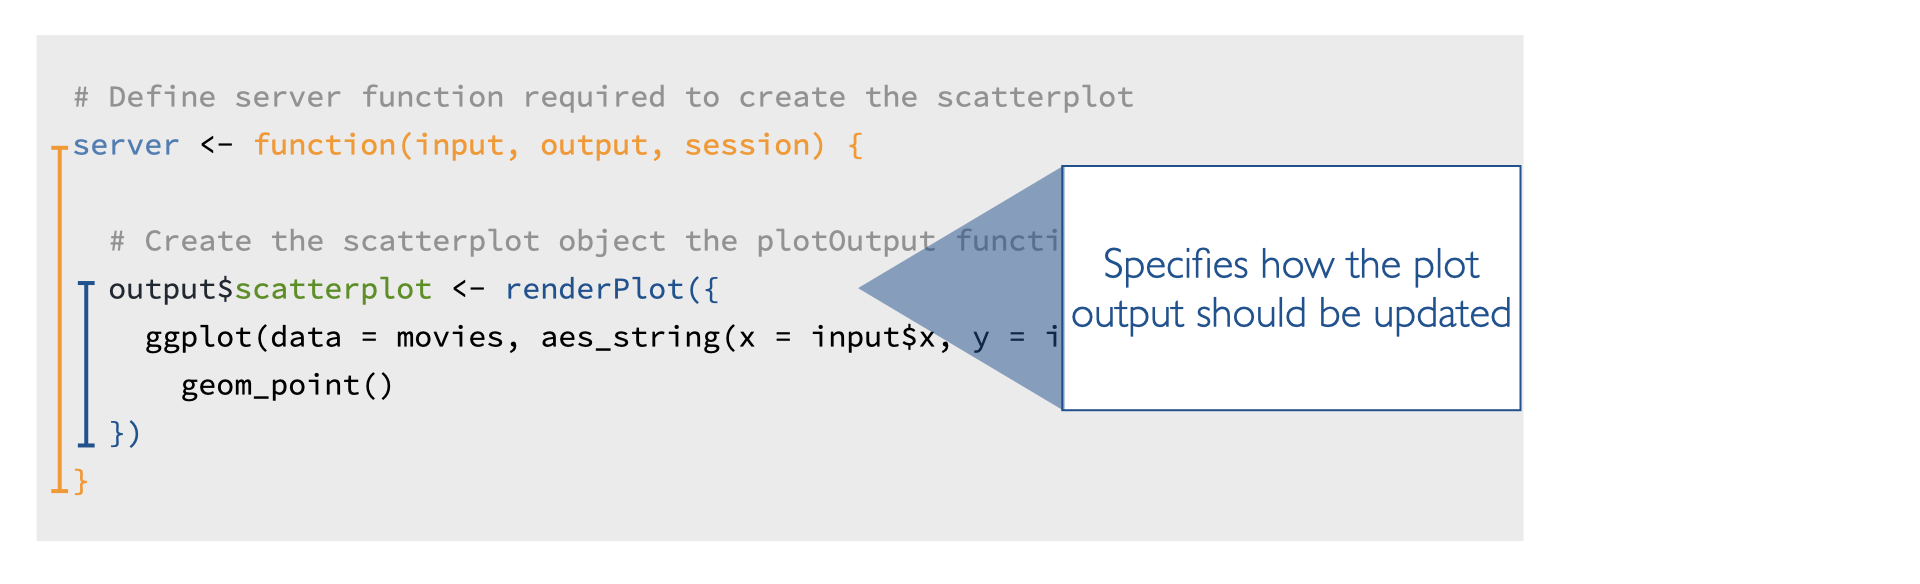
\includegraphics[width=1\textwidth,height=\textheight]{./images/output.png}

}

\end{figure}

The \texttt{renderPlot()} function specifies how the plot output should
be updated. Let's take a look at what is happening in the
\texttt{renderPlot()} function first.

\hypertarget{renderplot-1}{%
\subsection{\texorpdfstring{\texttt{renderPlot()}}{renderPlot()}}\label{renderplot-1}}

\begin{figure}

{\centering 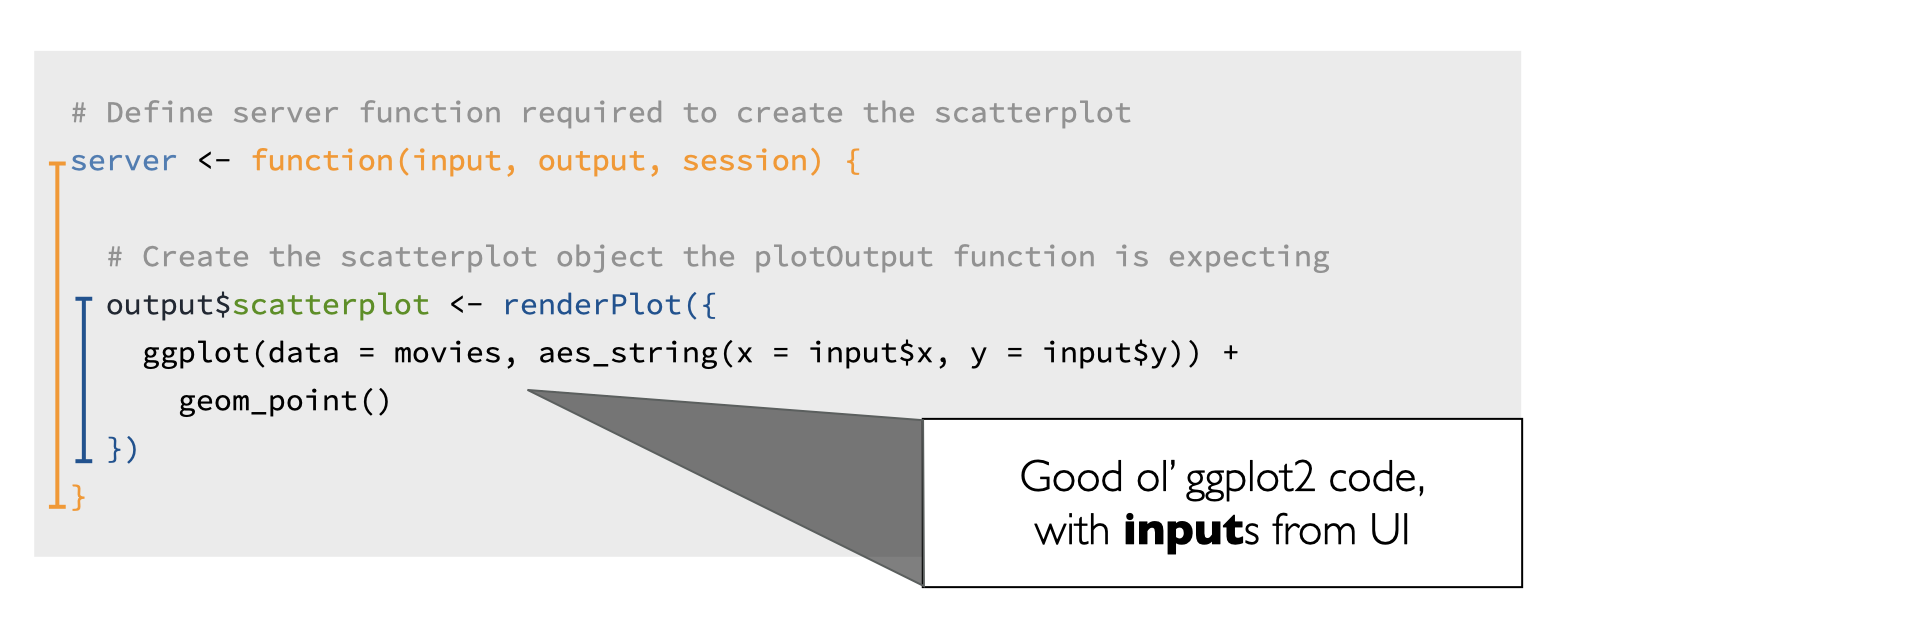
\includegraphics[width=1\textwidth,height=\textheight]{./images/renderplot.png}

}

\end{figure}

This is good ol' ggplot2 code! So even if you're new to shiny, if you've
previously used ggplot2 for plotting in R, this syntax should look
familiar to you.

One aspect of the syntax that might be new, however, is how the x and y
variables are defined. They come from the input list that is built in
the UI.

\hypertarget{inputs-1}{%
\subsection{Inputs}\label{inputs-1}}

Here is the relevant UI and server code.

\begin{figure}

{\centering 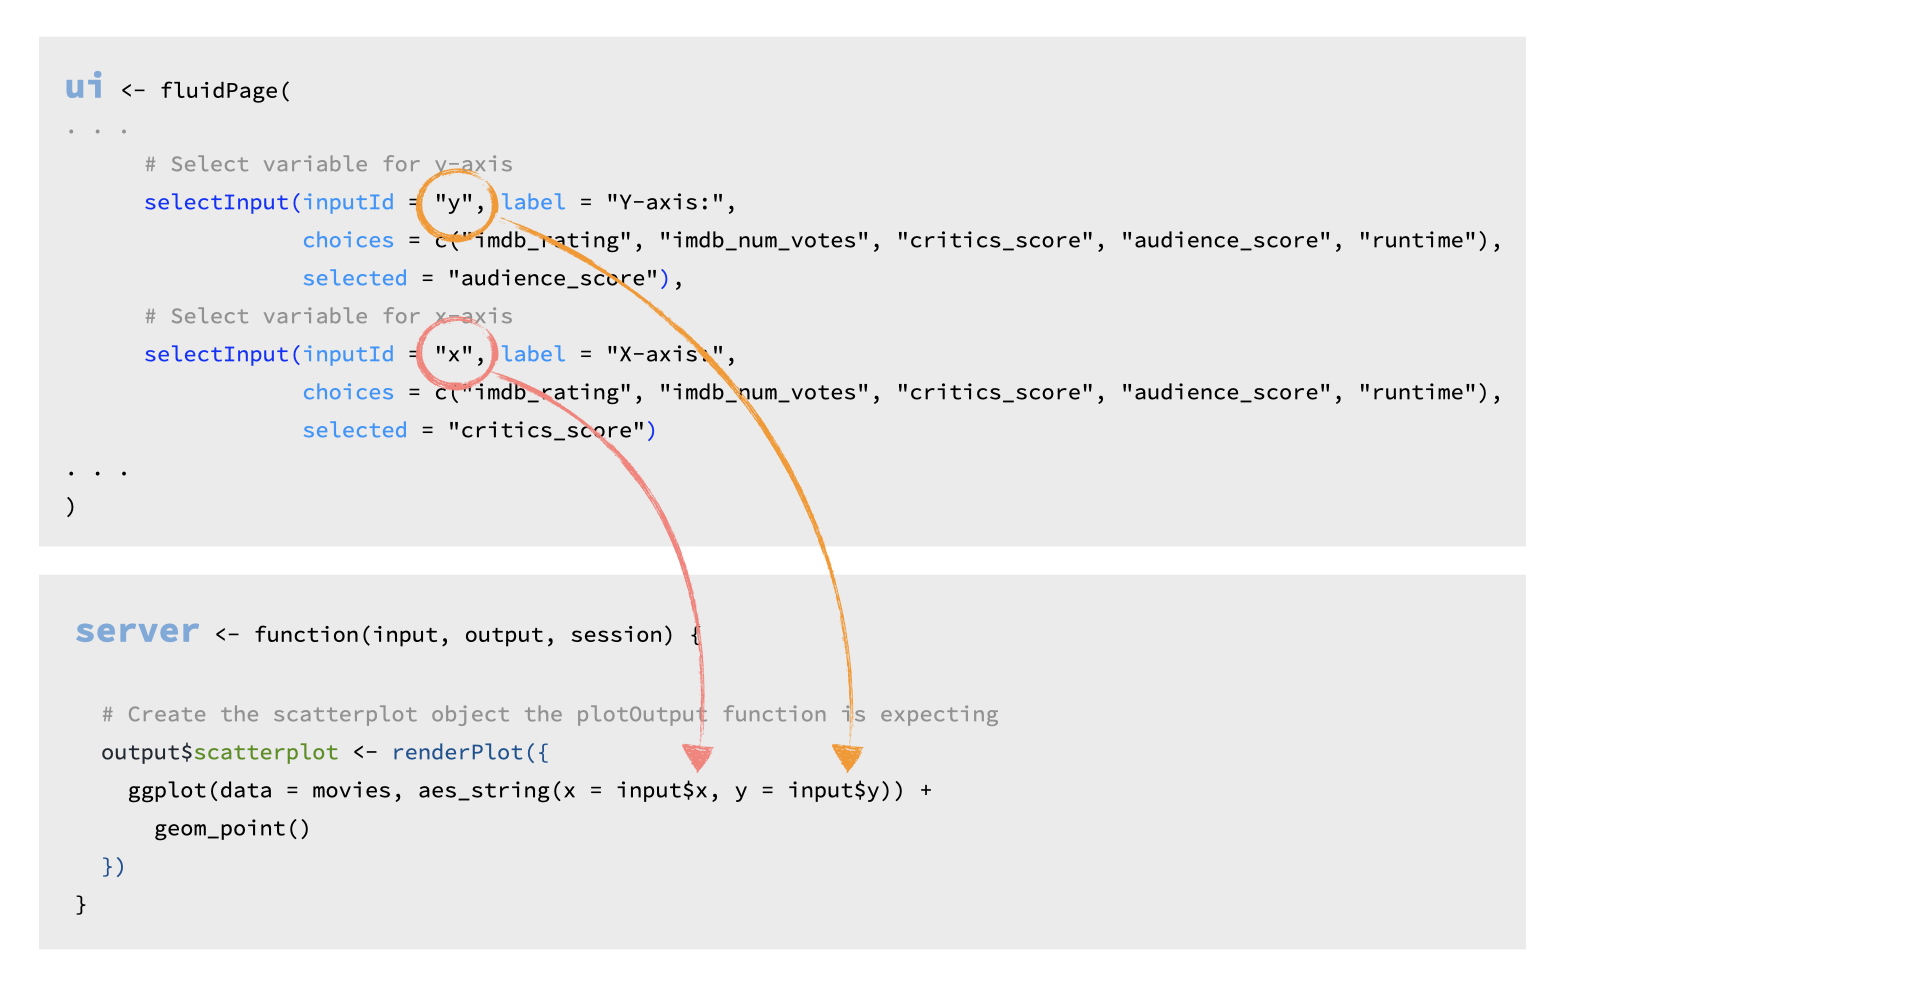
\includegraphics[width=1\textwidth,height=\textheight]{./images/inputs-x-y.png}

}

\end{figure}

Input x and y come from the \texttt{selectInput()} widgets, and map to
the \texttt{x} and \texttt{y} arguments of the plot aesthetics.

\hypertarget{rules-of-server-functions-1}{%
\subsection{Rules of server
functions}\label{rules-of-server-functions-1}}

There are three rules of building server functions:

\begin{enumerate}
\def\labelenumi{\arabic{enumi}.}
\item
  Always save objects to display to the named output list,
  i.e.~something of the form \texttt{output\$xx}, where \texttt{xx} is
  the plot you want to display.
\item
  Always build objects to display with one of the \texttt{render*()}
  functions, like we built our plot with \texttt{renderPlot()}.
\item
  Use input values from the named input list, with \texttt{input\$xx}.
\end{enumerate}

\hypertarget{output-types-1}{%
\subsection{Output types}\label{output-types-1}}

Just like various inputs, Shiny also provides a wide selection of output
types each of which works with a render function.

\begin{figure}

{\centering 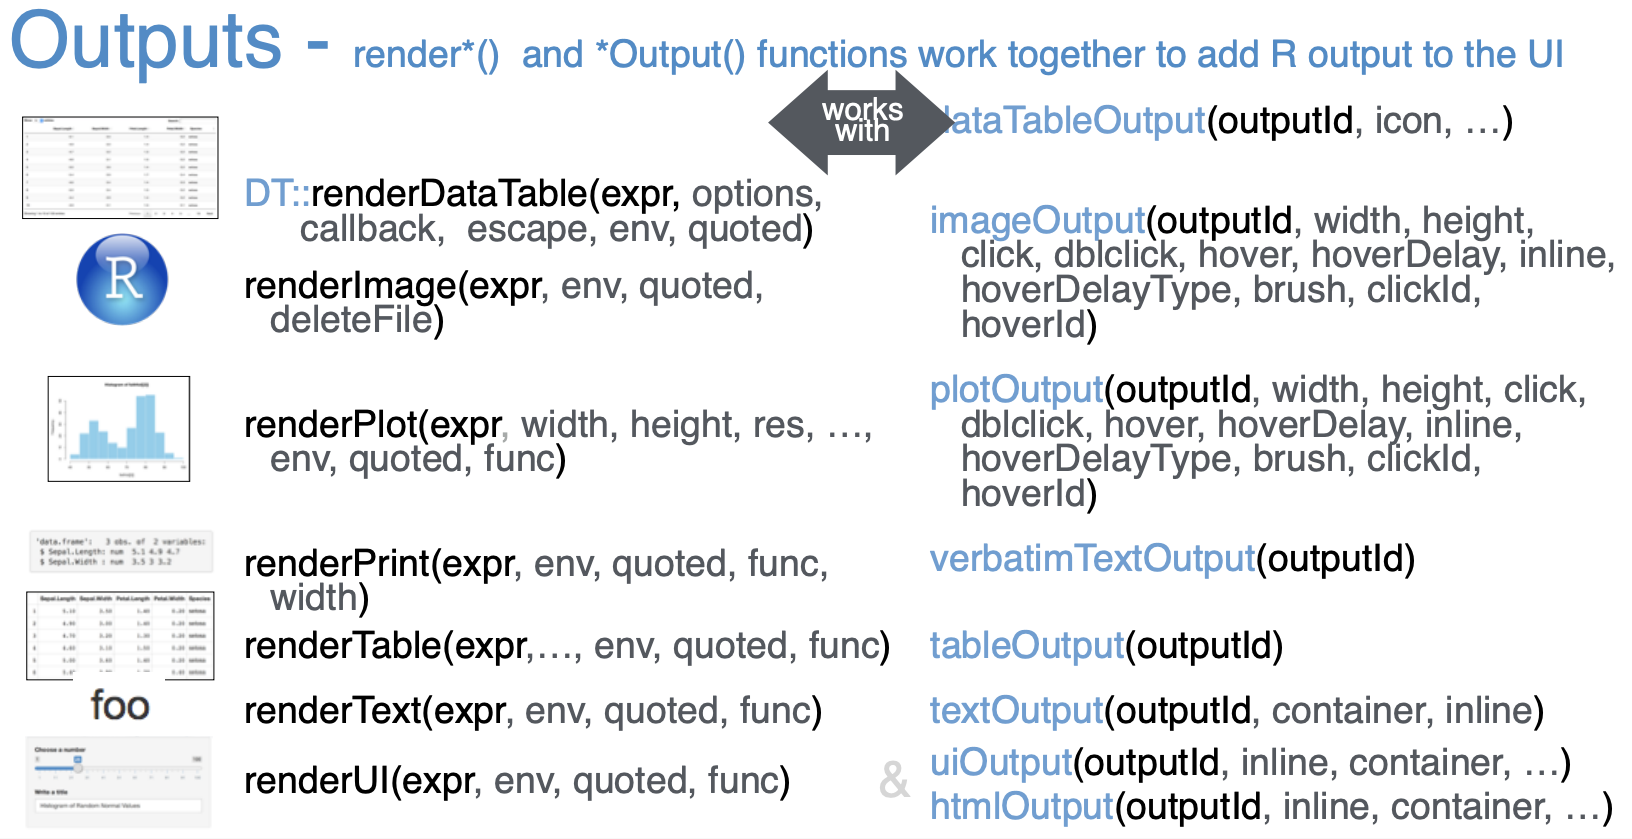
\includegraphics[width=0.8\textwidth,height=\textheight]{./images/cheatsheet-outputs.png}

}

\end{figure}

For example, in our app we used the \texttt{renderPlot()} function to
build our reactive plot (we'll get to what I mean by reactive in a
second) and laid out the plot with the \texttt{plotOutput()} function.

\begin{figure}

{\centering \includegraphics[width=1\textwidth,height=\textheight]{./images/render-output-pairs.png}

}

\end{figure}

Shiny knows to match these two together as they use the same
\texttt{outputID}, scatterplot.

In the following exercises you'll get a chance to work with other
render/output function pairs to add more elements to your app.

\hypertarget{practice-matching-inputs-and-outputs-1}{%
\subsection{Practice: Matching inputs and
outputs}\label{practice-matching-inputs-and-outputs-1}}

Here is a simple Shiny app. Try entering some text and observe how the
text is displayed back to you after a short pause.

\begin{center}\rule{0.5\linewidth}{0.5pt}\end{center}

\#\texttt{\{r,\ context\ =\ "server",\ eval\ =\ TRUE\}\ \#\ output\$user\_text\ \textless{}-\ renderText(\{\ input\$custom\_text\ \})\ \#}

\begin{center}\rule{0.5\linewidth}{0.5pt}\end{center}

The code for this app is given below, with a few pieces missing
(indicated with \texttt{\_\_\_}). Each of the blanks are numbered,
e.g.~(\texttt{{[}1{]}}, \texttt{{[}2{]}}, etc.)

\begin{Shaded}
\begin{Highlighting}[]
\FunctionTok{library}\NormalTok{(shiny)}

\NormalTok{ui }\OtherTok{\textless{}{-}} \FunctionTok{fluidPage}\NormalTok{(}

  \FunctionTok{textInput}\NormalTok{(}
    \AttributeTok{inputId =} \StringTok{"custom\_text"}\NormalTok{,}
    \AttributeTok{label =} \StringTok{"\_[1]\_"}
\NormalTok{  ),}

  \FunctionTok{strong}\NormalTok{(}\StringTok{"Text is shown below:"}\NormalTok{),}

\NormalTok{  \_[}\DecValTok{2}\NormalTok{]}\FunctionTok{\_}\NormalTok{(}\AttributeTok{outputId =} \StringTok{"\_[3]\_"}\NormalTok{)}

\NormalTok{)}

\NormalTok{server }\OtherTok{\textless{}{-}} \ControlFlowTok{function}\NormalTok{(input, output, session)\{}

\NormalTok{  output}\SpecialCharTok{$}\NormalTok{user\_text }\OtherTok{\textless{}{-}} \FunctionTok{renderText}\NormalTok{(\{ input}\SpecialCharTok{$}\NormalTok{\_[}\DecValTok{4}\NormalTok{]\_ \})}

\NormalTok{\}}

\FunctionTok{shinyApp}\NormalTok{(}\AttributeTok{ui =}\NormalTok{ ui, }\AttributeTok{server =}\NormalTok{ server)}
\end{Highlighting}
\end{Shaded}

\#\texttt{\{r\ mc-2\}\ \#question("Which\ of\ the\ following\ is\ false?",\ \#\ \ answer(\textquotesingle{}\textasciigrave{}{[}1{]}\textasciigrave{}\ should\ be\ \textasciigrave{}"Input\ some\ text\ here:"\textasciigrave{}\textquotesingle{},\ \#\ \ \ \ \ \ \ \ \ message\ =\ "Take\ a\ look\ at\ the\ app,\ what\ text\ is\ \#shown\ to\ the\ user\ above\ the\ text\ input\ area?"),\ \#\ \ answer(\textquotesingle{}\textasciigrave{}{[}2{]}\textasciigrave{}\ should\ be\ \textasciigrave{}textOutput\textasciigrave{}\textquotesingle{},\ \ \#\ \ \ \ \ \ \ \ \ message\ =\ "Check\ out\ the\ Shiny\ cheatsheet\ for\ pairs\ \#of\ input\ and\ output\ functions"),\ \#\ \ answer(\textquotesingle{}\textasciigrave{}{[}3{]}\textasciigrave{}\ should\ be\ \textasciigrave{}"custom\_text"\textasciigrave{}\textquotesingle{},\ correct\ =\ TRUE),\ \#\ \ answer(\textquotesingle{}\textasciigrave{}{[}4{]}\textasciigrave{}\ should\ be\ \textasciigrave{}"custom\_text"\textasciigrave{}\textquotesingle{},\ \#\ \ \ \ \ \ \ \ \ message\ =\ "What\ is\ the\ ID\ of\ the\ input\ that\ should\ \#be\ rendered?"),\ \#\ \ allow\_retry\ =\ TRUE\ \#)\ \#}

\hypertarget{reactivity-1}{%
\subsection{Reactivity}\label{reactivity-1}}

Let's also briefly discuss reactivity.

\begin{figure}

{\centering \includegraphics[width=0.8\textwidth,height=\textheight]{./images/reactivity.png}

}

\end{figure}

It's easy to build interactive applications with Shiny, but to get the
most out of it, you'll need to understand the reactive programming
scheme used by Shiny.

In a nutshell Shiny automatically updates outputs, such as plots, when
inputs that go into them change.

\hypertarget{putting-all-the-pieces-together-1}{%
\subsection{Putting all the pieces
together}\label{putting-all-the-pieces-together-1}}

Before we wrap up this section, I should also mention the last component
of each Shiny app, which is a call to the aptly named
\texttt{shinyApp()} function, which puts the UI and the server pieces
together to create a Shiny app object.

\begin{figure}

{\centering \includegraphics[width=0.8\textwidth,height=\textheight]{./images/shinyAppfunction.png}

}

\end{figure}

Time to put this all into practice!

\hypertarget{practice-rules-of-server-functions-1}{%
\subsection{Practice: Rules of server
functions}\label{practice-rules-of-server-functions-1}}

Which of the following is not true about server functions?

\#\texttt{\{r\ mc-3\}\ \#question("Which\ of\ the\ following\ is\ not\ true\ about\ server\ functions?",\ \#\ \ answer("Server\ functions\ should\ include\ a\ call\ to\ \#\textasciigrave{}runApp()\textasciigrave{}",\ \#\ \ \ \ correct\ =\ TRUE,\ \#\ \ \ \ message\ =\ "The\ \textasciigrave{}runApp()\textasciigrave{}\ function\ can\ be\ used\ in\ the\ Console\ to\ run\ a\ Shiny\ application,\ as\ an\ alternative\ to\ the\ Run\ App\ button\ in\ the\ RStudio\ IDE."\ \#\ \ ),\ \#\ \ answer("Objects\ to\ be\ displayed\ should\ be\ saved\ to\ \#\textasciigrave{}output\$\textasciigrave{}"),\ \#\ \ answer("Reactive\ objects\ should\ be\ built\ with\ \textasciigrave{}render*()\textasciigrave{}\ functions"),\ \#\ \ answer("Input\ values\ should\ be\ referred\ to\ with\ \textasciigrave{}input\$\textasciigrave{}"),\ \#\ \ allow\_retry\ =\ TRUE,\ \#\ \ random\_answer\_order\ =\ TRUE\ \#)\ \#}

\hypertarget{practice-fix-it-up-1}{%
\subsection{Practice: Fix it up}\label{practice-fix-it-up-1}}

Below is the code for the Shiny app we built earlier, however currently
the code is broken. Specifically there are errors in the definition of
the server function as well as in the \texttt{mainPanel} of the UI.

\hypertarget{your-turn-6}{%
\subsubsection{Your turn}\label{your-turn-6}}

\begin{itemize}
\tightlist
\item
  Review the app and identify errors in the code.

  \begin{itemize}
  \tightlist
  \item
    Hint: Refer back to the rules of server functions.
  \end{itemize}
\item
  Do the render functions match the output functions? If not, make the
  appropriate change and try running the app. Are there any remaining
  errors?
\item
  Are the inputs referred to using the correct syntax? If not, make the
  appropriate change and try running the app. Are there any remaining
  errors?
\item
  Are the outputs referred to using the correct names? If not, make the
  appropriate change and try running the app. Are there any remaining
  errors?
\end{itemize}

\emph{Navigate to the project called \textbf{1-3 Fix it up} after
clicking the button below}

\href{https://rstudio.cloud/spaces/81721/join?access_code=I4VJaNsKfTqR3Td9hLP7E1nz8\%2FtMg6Xbw9Bgqumv}{
Go to RStudio Cloud Workspace}

\begin{Shaded}
\begin{Highlighting}[]
\CommentTok{\# Load packages {-}{-}{-}{-}{-}{-}{-}{-}{-}{-}{-}{-}{-}{-}{-}{-}{-}{-}{-}{-}{-}{-}{-}{-}{-}{-}{-}{-}{-}{-}{-}{-}{-}{-}{-}{-}{-}{-}{-}{-}{-}{-}{-}{-}{-}{-}{-}{-}{-}{-}{-}{-}{-}{-}{-}{-}{-}{-}{-}{-}{-}{-}{-}{-}}

\FunctionTok{library}\NormalTok{(shiny)}
\FunctionTok{library}\NormalTok{(ggplot2)}

\CommentTok{\# Load data {-}{-}{-}{-}{-}{-}{-}{-}{-}{-}{-}{-}{-}{-}{-}{-}{-}{-}{-}{-}{-}{-}{-}{-}{-}{-}{-}{-}{-}{-}{-}{-}{-}{-}{-}{-}{-}{-}{-}{-}{-}{-}{-}{-}{-}{-}{-}{-}{-}{-}{-}{-}{-}{-}{-}{-}{-}{-}{-}{-}{-}{-}{-}{-}{-}{-}{-}{-}}

\FunctionTok{load}\NormalTok{(}\StringTok{"movies.RData"}\NormalTok{)}

\CommentTok{\# Define UI {-}{-}{-}{-}{-}{-}{-}{-}{-}{-}{-}{-}{-}{-}{-}{-}{-}{-}{-}{-}{-}{-}{-}{-}{-}{-}{-}{-}{-}{-}{-}{-}{-}{-}{-}{-}{-}{-}{-}{-}{-}{-}{-}{-}{-}{-}{-}{-}{-}{-}{-}{-}{-}{-}{-}{-}{-}{-}{-}{-}{-}{-}{-}{-}{-}{-}{-}{-}}

\NormalTok{ui }\OtherTok{\textless{}{-}} \FunctionTok{fluidPage}\NormalTok{(}
  \FunctionTok{sidebarLayout}\NormalTok{(}

    \CommentTok{\# Inputs: Select variables to plot}
    \FunctionTok{sidebarPanel}\NormalTok{(}

      \CommentTok{\# Select variable for y{-}axis}
      \FunctionTok{selectInput}\NormalTok{(}
        \AttributeTok{inputId =} \StringTok{"y"}\NormalTok{,}
        \AttributeTok{label =} \StringTok{"Y{-}axis:"}\NormalTok{,}
        \AttributeTok{choices =} \FunctionTok{c}\NormalTok{(}
          \StringTok{"IMDB rating"} \OtherTok{=} \StringTok{"imdb\_rating"}\NormalTok{,}
          \StringTok{"IMDB number of votes"} \OtherTok{=} \StringTok{"imdb\_num\_votes"}\NormalTok{,}
          \StringTok{"Critics score"} \OtherTok{=} \StringTok{"critics\_score"}\NormalTok{,}
          \StringTok{"Audience score"} \OtherTok{=} \StringTok{"audience\_score"}\NormalTok{,}
          \StringTok{"Runtime"} \OtherTok{=} \StringTok{"runtime"}
\NormalTok{        ),}
        \AttributeTok{selected =} \StringTok{"audience\_score"}
\NormalTok{      ),}

      \CommentTok{\# Select variable for x{-}axis}
      \FunctionTok{selectInput}\NormalTok{(}
        \AttributeTok{inputId =} \StringTok{"x"}\NormalTok{,}
        \AttributeTok{label =} \StringTok{"X{-}axis:"}\NormalTok{,}
        \AttributeTok{choices =} \FunctionTok{c}\NormalTok{(}
          \StringTok{"IMDB rating"} \OtherTok{=} \StringTok{"imdb\_rating"}\NormalTok{,}
          \StringTok{"IMDB number of votes"} \OtherTok{=} \StringTok{"imdb\_num\_votes"}\NormalTok{,}
          \StringTok{"Critics score"} \OtherTok{=} \StringTok{"critics\_score"}\NormalTok{,}
          \StringTok{"Audience score"} \OtherTok{=} \StringTok{"audience\_score"}\NormalTok{,}
          \StringTok{"Runtime"} \OtherTok{=} \StringTok{"runtime"}
\NormalTok{        ),}
        \AttributeTok{selected =} \StringTok{"critics\_score"}
\NormalTok{      ),}

      \CommentTok{\# Select variable for color}
      \FunctionTok{selectInput}\NormalTok{(}
        \AttributeTok{inputId =} \StringTok{"z"}\NormalTok{,}
        \AttributeTok{label =} \StringTok{"Color by:"}\NormalTok{,}
        \AttributeTok{choices =} \FunctionTok{c}\NormalTok{(}
          \StringTok{"Title type"} \OtherTok{=} \StringTok{"title\_type"}\NormalTok{,}
          \StringTok{"Genre"} \OtherTok{=} \StringTok{"genre"}\NormalTok{,}
          \StringTok{"MPAA rating"} \OtherTok{=} \StringTok{"mpaa\_rating"}\NormalTok{,}
          \StringTok{"Critics rating"} \OtherTok{=} \StringTok{"critics\_rating"}\NormalTok{,}
          \StringTok{"Audience rating"} \OtherTok{=} \StringTok{"audience\_rating"}
\NormalTok{        ),}
        \AttributeTok{selected =} \StringTok{"mpaa\_rating"}
\NormalTok{      )}
\NormalTok{    ),}

    \CommentTok{\# Output: Show scatterplot}
    \FunctionTok{mainPanel}\NormalTok{(}
      \FunctionTok{plotOutput}\NormalTok{(}\AttributeTok{outputId =} \StringTok{"scatterPlot"}\NormalTok{)}
\NormalTok{    )}
\NormalTok{  )}
\NormalTok{)}

\CommentTok{\# Define server {-}{-}{-}{-}{-}{-}{-}{-}{-}{-}{-}{-}{-}{-}{-}{-}{-}{-}{-}{-}{-}{-}{-}{-}{-}{-}{-}{-}{-}{-}{-}{-}{-}{-}{-}{-}{-}{-}{-}{-}{-}{-}{-}{-}{-}{-}{-}{-}{-}{-}{-}{-}{-}{-}{-}{-}{-}{-}{-}{-}{-}{-}{-}{-}}

\NormalTok{server }\OtherTok{\textless{}{-}} \ControlFlowTok{function}\NormalTok{(input, output, session) \{}
\NormalTok{  output}\SpecialCharTok{$}\NormalTok{scatterplot }\OtherTok{\textless{}{-}} \FunctionTok{renderTable}\NormalTok{(\{}

    \FunctionTok{ggplot}\NormalTok{(}\AttributeTok{data =}\NormalTok{ movies, }\FunctionTok{aes\_string}\NormalTok{(}\AttributeTok{x =}\NormalTok{ x, }\AttributeTok{y =}\NormalTok{ y, }\AttributeTok{color =}\NormalTok{ z)) }\SpecialCharTok{+}
      \FunctionTok{geom\_point}\NormalTok{()}

\NormalTok{  \})}

\NormalTok{\}}

\CommentTok{\# Create a Shiny app object {-}{-}{-}{-}{-}{-}{-}{-}{-}{-}{-}{-}{-}{-}{-}{-}{-}{-}{-}{-}{-}{-}{-}{-}{-}{-}{-}{-}{-}{-}{-}{-}{-}{-}{-}{-}{-}{-}{-}{-}{-}{-}{-}{-}{-}{-}{-}{-}{-}{-}{-}{-}}

\FunctionTok{shinyApp}\NormalTok{(}\AttributeTok{ui =}\NormalTok{ ui, }\AttributeTok{server =}\NormalTok{ server)}
\end{Highlighting}
\end{Shaded}

\hypertarget{recap-1}{%
\section{Recap}\label{recap-1}}

Let's quickly recap what we have learned in this chapter.

\hypertarget{section-12}{%
\subsection{}\label{section-12}}

Every Shiny app has a webpage that the user visits, and behind this
webpage there is a computer that serves this webpage by running R.

\begin{figure}

{\centering \includegraphics[width=0.8\textwidth,height=\textheight]{./images/recap-1.png}

}

\end{figure}

\hypertarget{section-13}{%
\subsection{}\label{section-13}}

When running your app locally, the computer serving your app is your
computer.

\begin{figure}

{\centering \includegraphics[width=0.8\textwidth,height=\textheight]{./images/recap-2.png}

}

\end{figure}

\hypertarget{section-14}{%
\subsection{}\label{section-14}}

When your app is deployed, the computer serving your app is a web
server.

\begin{figure}

{\centering \includegraphics[width=0.8\textwidth,height=\textheight]{./images/recap-3.png}

}

\end{figure}

\hypertarget{section-15}{%
\subsection{}\label{section-15}}

Each app is comprised of two components, a UI and a server.

\begin{figure}

{\centering \includegraphics[width=0.8\textwidth,height=\textheight]{./images/recap-4.png}

}

\end{figure}

\begin{itemize}
\item
  The UI is ultimately built with HTML, CSS, and JavaScript. However,
  you as the Shiny developer do not need to know these languages. Shiny
  lets R users write user interfaces using a simple, familiar-looking
  API. However there are no limits to customization for advanced users
  who are familiar with these languages.
\item
  The server function contains the instructions to map user inputs to
  outputs.
\end{itemize}

I often think of the UI as containing syntax specific to Shiny, and the
server as containing R code you might already be familiar with -- with
some Shiny functions added to achieve reactivity.

\hypertarget{tip-change-display-1}{%
\subsection{Tip: Change display}\label{tip-change-display-1}}

In this tutorial you will be developing your apps in RStudio Cloud
projects, but once you're done with the tutorial you might consider
developing your apps in the RStudio IDE, which has some some handy-dandy
functionality for running and viewing your apps.

RStudio will automatically recognize R scripts that contain \texttt{ui}
and \texttt{server} components and that end with a call to the
\texttt{shinyApp()} function and will make available the Run App button.
You can choose to run your app in a new window, or in the viewer pane of
your RStudio window.

\begin{figure}

{\centering \includegraphics[width=0.8\textwidth,height=\textheight]{./images/recap-5.png}

}

\end{figure}

\hypertarget{tip-close-an-app-1}{%
\subsection{Tip: Close an app}\label{tip-close-an-app-1}}

When you are done with an app, you can terminate the session by clicking
the red stop button in your viewer pane.

\begin{figure}

{\centering \includegraphics[width=0.8\textwidth,height=\textheight]{./images/recap-6.png}

}

\end{figure}

\hypertarget{section-16}{%
\subsection{}\label{section-16}}

That's all for this module! In the next module we discuss inputs,
outputs, and rendering functions in further detail.

\hypertarget{server-function-2}{%
\chapter{Server function}\label{server-function-2}}

Now that you've had some practice with the UI, it's time to move on to
the server function.

Again, before we get into the details, let's remind ourselves of the
anatomy of a Shiny app. The basic task of the server function is to
define the relationship between inputs and outputs.

\hypertarget{here-again-is-the-app-that-we-are-working-with-in-this-module-2}{%
\subsection{Here again is the app that we are working with in this
module}\label{here-again-is-the-app-that-we-are-working-with-in-this-module-2}}

Earlier we saw how to build the UI of this app, and we also noted that
each input was tagged with an \texttt{inputId} that can be used to refer
to them in the server.

\begin{figure}

{\centering \includegraphics[width=1\textwidth,height=\textheight]{./images/app-selectinput-scatterplot.png}

}

\end{figure}

\hypertarget{this-is-the-server-function-code-for-this-app-2}{%
\subsection{This is the server function code for this
app}\label{this-is-the-server-function-code-for-this-app-2}}

Once again there is a lot going on here to parse at once, so in the
following sections we take a closer look at the function.

\begin{figure}

{\centering \includegraphics[width=1\textwidth,height=\textheight]{./images/server.png}

}

\end{figure}

\hypertarget{at-the-outermost-layer-2}{%
\subsection{At the outermost layer}\label{at-the-outermost-layer-2}}

\begin{figure}

{\centering \includegraphics[width=1\textwidth,height=\textheight]{./images/server-outermost.png}

}

\end{figure}

We define our server function which takes two arguments: an
\texttt{input} and an \texttt{output}. Both of these are named lists.

The server function accesses inputs selected by the user to perform
computations and specifies how outputs laid out in the UI should be
updated.

The server function can take on one more argument, \texttt{session},
which is an environment that can be used to access information and
functionality relating to the session. However this concept is beyond
the scope of this tutorial, so for now we'll stick to server functions
that only have input and output arguments.

\hypertarget{output-2}{%
\subsection{\texorpdfstring{\texttt{output}}{output}}\label{output-2}}

Our simple app had only one output -- a plot. So our server function
contains the logic necessary to build this plot.

\begin{figure}

{\centering \includegraphics[width=1\textwidth,height=\textheight]{./images/output.png}

}

\end{figure}

The \texttt{renderPlot()} function specifies how the plot output should
be updated. Let's take a look at what is happening in the
\texttt{renderPlot()} function first.

\hypertarget{renderplot-2}{%
\subsection{\texorpdfstring{\texttt{renderPlot()}}{renderPlot()}}\label{renderplot-2}}

\begin{figure}

{\centering \includegraphics[width=1\textwidth,height=\textheight]{./images/renderplot.png}

}

\end{figure}

This is good ol' ggplot2 code! So even if you're new to shiny, if you've
previously used ggplot2 for plotting in R, this syntax should look
familiar to you.

One aspect of the syntax that might be new, however, is how the x and y
variables are defined. They come from the input list that is built in
the UI.

\hypertarget{inputs-2}{%
\subsection{Inputs}\label{inputs-2}}

Here is the relevant UI and server code.

\begin{figure}

{\centering \includegraphics[width=1\textwidth,height=\textheight]{./images/inputs-x-y.png}

}

\end{figure}

Input x and y come from the \texttt{selectInput()} widgets, and map to
the \texttt{x} and \texttt{y} arguments of the plot aesthetics.

\hypertarget{rules-of-server-functions-2}{%
\subsection{Rules of server
functions}\label{rules-of-server-functions-2}}

There are three rules of building server functions:

\begin{enumerate}
\def\labelenumi{\arabic{enumi}.}
\item
  Always save objects to display to the named output list,
  i.e.~something of the form \texttt{output\$xx}, where \texttt{xx} is
  the plot you want to display.
\item
  Always build objects to display with one of the \texttt{render*()}
  functions, like we built our plot with \texttt{renderPlot()}.
\item
  Use input values from the named input list, with \texttt{input\$xx}.
\end{enumerate}

\hypertarget{output-types-2}{%
\subsection{Output types}\label{output-types-2}}

Just like various inputs, Shiny also provides a wide selection of output
types each of which works with a render function.

\begin{figure}

{\centering \includegraphics[width=0.8\textwidth,height=\textheight]{./images/cheatsheet-outputs.png}

}

\end{figure}

For example, in our app we used the \texttt{renderPlot()} function to
build our reactive plot (we'll get to what I mean by reactive in a
second) and laid out the plot with the \texttt{plotOutput()} function.

\begin{figure}

{\centering \includegraphics[width=1\textwidth,height=\textheight]{./images/render-output-pairs.png}

}

\end{figure}

Shiny knows to match these two together as they use the same
\texttt{outputID}, scatterplot.

In the following exercises you'll get a chance to work with other
render/output function pairs to add more elements to your app.

\hypertarget{practice-matching-inputs-and-outputs-2}{%
\subsection{Practice: Matching inputs and
outputs}\label{practice-matching-inputs-and-outputs-2}}

Here is a simple Shiny app. Try entering some text and observe how the
text is displayed back to you after a short pause.

\begin{center}\rule{0.5\linewidth}{0.5pt}\end{center}

\#\texttt{\{r,\ context\ =\ "server",\ eval\ =\ TRUE\}\ \#\ output\$user\_text\ \textless{}-\ renderText(\{\ input\$custom\_text\ \})\ \#}

\begin{center}\rule{0.5\linewidth}{0.5pt}\end{center}

The code for this app is given below, with a few pieces missing
(indicated with \texttt{\_\_\_}). Each of the blanks are numbered,
e.g.~(\texttt{{[}1{]}}, \texttt{{[}2{]}}, etc.)

\begin{Shaded}
\begin{Highlighting}[]
\FunctionTok{library}\NormalTok{(shiny)}

\NormalTok{ui }\OtherTok{\textless{}{-}} \FunctionTok{fluidPage}\NormalTok{(}

  \FunctionTok{textInput}\NormalTok{(}
    \AttributeTok{inputId =} \StringTok{"custom\_text"}\NormalTok{,}
    \AttributeTok{label =} \StringTok{"\_[1]\_"}
\NormalTok{  ),}

  \FunctionTok{strong}\NormalTok{(}\StringTok{"Text is shown below:"}\NormalTok{),}

\NormalTok{  \_[}\DecValTok{2}\NormalTok{]}\FunctionTok{\_}\NormalTok{(}\AttributeTok{outputId =} \StringTok{"\_[3]\_"}\NormalTok{)}

\NormalTok{)}

\NormalTok{server }\OtherTok{\textless{}{-}} \ControlFlowTok{function}\NormalTok{(input, output, session)\{}

\NormalTok{  output}\SpecialCharTok{$}\NormalTok{user\_text }\OtherTok{\textless{}{-}} \FunctionTok{renderText}\NormalTok{(\{ input}\SpecialCharTok{$}\NormalTok{\_[}\DecValTok{4}\NormalTok{]\_ \})}

\NormalTok{\}}

\FunctionTok{shinyApp}\NormalTok{(}\AttributeTok{ui =}\NormalTok{ ui, }\AttributeTok{server =}\NormalTok{ server)}
\end{Highlighting}
\end{Shaded}

\#\texttt{\{r\ mc-2\}\ \#question("Which\ of\ the\ following\ is\ false?",\ \#\ \ answer(\textquotesingle{}\textasciigrave{}{[}1{]}\textasciigrave{}\ should\ be\ \textasciigrave{}"Input\ some\ text\ here:"\textasciigrave{}\textquotesingle{},\ \#\ \ \ \ \ \ \ \ \ message\ =\ "Take\ a\ look\ at\ the\ app,\ what\ text\ is\ \#shown\ to\ the\ user\ above\ the\ text\ input\ area?"),\ \#\ \ answer(\textquotesingle{}\textasciigrave{}{[}2{]}\textasciigrave{}\ should\ be\ \textasciigrave{}textOutput\textasciigrave{}\textquotesingle{},\ \ \#\ \ \ \ \ \ \ \ \ message\ =\ "Check\ out\ the\ Shiny\ cheatsheet\ for\ pairs\ \#of\ input\ and\ output\ functions"),\ \#\ \ answer(\textquotesingle{}\textasciigrave{}{[}3{]}\textasciigrave{}\ should\ be\ \textasciigrave{}"custom\_text"\textasciigrave{}\textquotesingle{},\ correct\ =\ TRUE),\ \#\ \ answer(\textquotesingle{}\textasciigrave{}{[}4{]}\textasciigrave{}\ should\ be\ \textasciigrave{}"custom\_text"\textasciigrave{}\textquotesingle{},\ \#\ \ \ \ \ \ \ \ \ message\ =\ "What\ is\ the\ ID\ of\ the\ input\ that\ should\ \#be\ rendered?"),\ \#\ \ allow\_retry\ =\ TRUE\ \#)\ \#}

\hypertarget{reactivity-2}{%
\subsection{Reactivity}\label{reactivity-2}}

Let's also briefly discuss reactivity.

\begin{figure}

{\centering \includegraphics[width=0.8\textwidth,height=\textheight]{./images/reactivity.png}

}

\end{figure}

It's easy to build interactive applications with Shiny, but to get the
most out of it, you'll need to understand the reactive programming
scheme used by Shiny.

In a nutshell Shiny automatically updates outputs, such as plots, when
inputs that go into them change.

\hypertarget{putting-all-the-pieces-together-2}{%
\subsection{Putting all the pieces
together}\label{putting-all-the-pieces-together-2}}

Before we wrap up this section, I should also mention the last component
of each Shiny app, which is a call to the aptly named
\texttt{shinyApp()} function, which puts the UI and the server pieces
together to create a Shiny app object.

\begin{figure}

{\centering \includegraphics[width=0.8\textwidth,height=\textheight]{./images/shinyAppfunction.png}

}

\end{figure}

Time to put this all into practice!

\hypertarget{practice-rules-of-server-functions-2}{%
\subsection{Practice: Rules of server
functions}\label{practice-rules-of-server-functions-2}}

Which of the following is not true about server functions?

\#\texttt{\{r\ mc-3\}\ \#question("Which\ of\ the\ following\ is\ not\ true\ about\ server\ functions?",\ \#\ \ answer("Server\ functions\ should\ include\ a\ call\ to\ \#\textasciigrave{}runApp()\textasciigrave{}",\ \#\ \ \ \ correct\ =\ TRUE,\ \#\ \ \ \ message\ =\ "The\ \textasciigrave{}runApp()\textasciigrave{}\ function\ can\ be\ used\ in\ the\ Console\ to\ run\ a\ Shiny\ application,\ as\ an\ alternative\ to\ the\ Run\ App\ button\ in\ the\ RStudio\ IDE."\ \#\ \ ),\ \#\ \ answer("Objects\ to\ be\ displayed\ should\ be\ saved\ to\ \#\textasciigrave{}output\$\textasciigrave{}"),\ \#\ \ answer("Reactive\ objects\ should\ be\ built\ with\ \textasciigrave{}render*()\textasciigrave{}\ functions"),\ \#\ \ answer("Input\ values\ should\ be\ referred\ to\ with\ \textasciigrave{}input\$\textasciigrave{}"),\ \#\ \ allow\_retry\ =\ TRUE,\ \#\ \ random\_answer\_order\ =\ TRUE\ \#)\ \#}

\hypertarget{practice-fix-it-up-2}{%
\subsection{Practice: Fix it up}\label{practice-fix-it-up-2}}

Below is the code for the Shiny app we built earlier, however currently
the code is broken. Specifically there are errors in the definition of
the server function as well as in the \texttt{mainPanel} of the UI.

\hypertarget{your-turn-7}{%
\subsubsection{Your turn}\label{your-turn-7}}

\begin{itemize}
\tightlist
\item
  Review the app and identify errors in the code.

  \begin{itemize}
  \tightlist
  \item
    Hint: Refer back to the rules of server functions.
  \end{itemize}
\item
  Do the render functions match the output functions? If not, make the
  appropriate change and try running the app. Are there any remaining
  errors?
\item
  Are the inputs referred to using the correct syntax? If not, make the
  appropriate change and try running the app. Are there any remaining
  errors?
\item
  Are the outputs referred to using the correct names? If not, make the
  appropriate change and try running the app. Are there any remaining
  errors?
\end{itemize}

\emph{Navigate to the project called \textbf{1-3 Fix it up} after
clicking the button below}

\href{https://rstudio.cloud/spaces/81721/join?access_code=I4VJaNsKfTqR3Td9hLP7E1nz8\%2FtMg6Xbw9Bgqumv}{
Go to RStudio Cloud Workspace}

\begin{Shaded}
\begin{Highlighting}[]
\CommentTok{\# Load packages {-}{-}{-}{-}{-}{-}{-}{-}{-}{-}{-}{-}{-}{-}{-}{-}{-}{-}{-}{-}{-}{-}{-}{-}{-}{-}{-}{-}{-}{-}{-}{-}{-}{-}{-}{-}{-}{-}{-}{-}{-}{-}{-}{-}{-}{-}{-}{-}{-}{-}{-}{-}{-}{-}{-}{-}{-}{-}{-}{-}{-}{-}{-}{-}}

\FunctionTok{library}\NormalTok{(shiny)}
\FunctionTok{library}\NormalTok{(ggplot2)}

\CommentTok{\# Load data {-}{-}{-}{-}{-}{-}{-}{-}{-}{-}{-}{-}{-}{-}{-}{-}{-}{-}{-}{-}{-}{-}{-}{-}{-}{-}{-}{-}{-}{-}{-}{-}{-}{-}{-}{-}{-}{-}{-}{-}{-}{-}{-}{-}{-}{-}{-}{-}{-}{-}{-}{-}{-}{-}{-}{-}{-}{-}{-}{-}{-}{-}{-}{-}{-}{-}{-}{-}}

\FunctionTok{load}\NormalTok{(}\StringTok{"movies.RData"}\NormalTok{)}

\CommentTok{\# Define UI {-}{-}{-}{-}{-}{-}{-}{-}{-}{-}{-}{-}{-}{-}{-}{-}{-}{-}{-}{-}{-}{-}{-}{-}{-}{-}{-}{-}{-}{-}{-}{-}{-}{-}{-}{-}{-}{-}{-}{-}{-}{-}{-}{-}{-}{-}{-}{-}{-}{-}{-}{-}{-}{-}{-}{-}{-}{-}{-}{-}{-}{-}{-}{-}{-}{-}{-}{-}}

\NormalTok{ui }\OtherTok{\textless{}{-}} \FunctionTok{fluidPage}\NormalTok{(}
  \FunctionTok{sidebarLayout}\NormalTok{(}

    \CommentTok{\# Inputs: Select variables to plot}
    \FunctionTok{sidebarPanel}\NormalTok{(}

      \CommentTok{\# Select variable for y{-}axis}
      \FunctionTok{selectInput}\NormalTok{(}
        \AttributeTok{inputId =} \StringTok{"y"}\NormalTok{,}
        \AttributeTok{label =} \StringTok{"Y{-}axis:"}\NormalTok{,}
        \AttributeTok{choices =} \FunctionTok{c}\NormalTok{(}
          \StringTok{"IMDB rating"} \OtherTok{=} \StringTok{"imdb\_rating"}\NormalTok{,}
          \StringTok{"IMDB number of votes"} \OtherTok{=} \StringTok{"imdb\_num\_votes"}\NormalTok{,}
          \StringTok{"Critics score"} \OtherTok{=} \StringTok{"critics\_score"}\NormalTok{,}
          \StringTok{"Audience score"} \OtherTok{=} \StringTok{"audience\_score"}\NormalTok{,}
          \StringTok{"Runtime"} \OtherTok{=} \StringTok{"runtime"}
\NormalTok{        ),}
        \AttributeTok{selected =} \StringTok{"audience\_score"}
\NormalTok{      ),}

      \CommentTok{\# Select variable for x{-}axis}
      \FunctionTok{selectInput}\NormalTok{(}
        \AttributeTok{inputId =} \StringTok{"x"}\NormalTok{,}
        \AttributeTok{label =} \StringTok{"X{-}axis:"}\NormalTok{,}
        \AttributeTok{choices =} \FunctionTok{c}\NormalTok{(}
          \StringTok{"IMDB rating"} \OtherTok{=} \StringTok{"imdb\_rating"}\NormalTok{,}
          \StringTok{"IMDB number of votes"} \OtherTok{=} \StringTok{"imdb\_num\_votes"}\NormalTok{,}
          \StringTok{"Critics score"} \OtherTok{=} \StringTok{"critics\_score"}\NormalTok{,}
          \StringTok{"Audience score"} \OtherTok{=} \StringTok{"audience\_score"}\NormalTok{,}
          \StringTok{"Runtime"} \OtherTok{=} \StringTok{"runtime"}
\NormalTok{        ),}
        \AttributeTok{selected =} \StringTok{"critics\_score"}
\NormalTok{      ),}

      \CommentTok{\# Select variable for color}
      \FunctionTok{selectInput}\NormalTok{(}
        \AttributeTok{inputId =} \StringTok{"z"}\NormalTok{,}
        \AttributeTok{label =} \StringTok{"Color by:"}\NormalTok{,}
        \AttributeTok{choices =} \FunctionTok{c}\NormalTok{(}
          \StringTok{"Title type"} \OtherTok{=} \StringTok{"title\_type"}\NormalTok{,}
          \StringTok{"Genre"} \OtherTok{=} \StringTok{"genre"}\NormalTok{,}
          \StringTok{"MPAA rating"} \OtherTok{=} \StringTok{"mpaa\_rating"}\NormalTok{,}
          \StringTok{"Critics rating"} \OtherTok{=} \StringTok{"critics\_rating"}\NormalTok{,}
          \StringTok{"Audience rating"} \OtherTok{=} \StringTok{"audience\_rating"}
\NormalTok{        ),}
        \AttributeTok{selected =} \StringTok{"mpaa\_rating"}
\NormalTok{      )}
\NormalTok{    ),}

    \CommentTok{\# Output: Show scatterplot}
    \FunctionTok{mainPanel}\NormalTok{(}
      \FunctionTok{plotOutput}\NormalTok{(}\AttributeTok{outputId =} \StringTok{"scatterPlot"}\NormalTok{)}
\NormalTok{    )}
\NormalTok{  )}
\NormalTok{)}

\CommentTok{\# Define server {-}{-}{-}{-}{-}{-}{-}{-}{-}{-}{-}{-}{-}{-}{-}{-}{-}{-}{-}{-}{-}{-}{-}{-}{-}{-}{-}{-}{-}{-}{-}{-}{-}{-}{-}{-}{-}{-}{-}{-}{-}{-}{-}{-}{-}{-}{-}{-}{-}{-}{-}{-}{-}{-}{-}{-}{-}{-}{-}{-}{-}{-}{-}{-}}

\NormalTok{server }\OtherTok{\textless{}{-}} \ControlFlowTok{function}\NormalTok{(input, output, session) \{}
\NormalTok{  output}\SpecialCharTok{$}\NormalTok{scatterplot }\OtherTok{\textless{}{-}} \FunctionTok{renderTable}\NormalTok{(\{}

    \FunctionTok{ggplot}\NormalTok{(}\AttributeTok{data =}\NormalTok{ movies, }\FunctionTok{aes\_string}\NormalTok{(}\AttributeTok{x =}\NormalTok{ x, }\AttributeTok{y =}\NormalTok{ y, }\AttributeTok{color =}\NormalTok{ z)) }\SpecialCharTok{+}
      \FunctionTok{geom\_point}\NormalTok{()}

\NormalTok{  \})}

\NormalTok{\}}

\CommentTok{\# Create a Shiny app object {-}{-}{-}{-}{-}{-}{-}{-}{-}{-}{-}{-}{-}{-}{-}{-}{-}{-}{-}{-}{-}{-}{-}{-}{-}{-}{-}{-}{-}{-}{-}{-}{-}{-}{-}{-}{-}{-}{-}{-}{-}{-}{-}{-}{-}{-}{-}{-}{-}{-}{-}{-}}

\FunctionTok{shinyApp}\NormalTok{(}\AttributeTok{ui =}\NormalTok{ ui, }\AttributeTok{server =}\NormalTok{ server)}
\end{Highlighting}
\end{Shaded}

\hypertarget{recap-2}{%
\section{Recap}\label{recap-2}}

Let's quickly recap what we have learned in this chapter.

\hypertarget{section-17}{%
\subsection{}\label{section-17}}

Every Shiny app has a webpage that the user visits, and behind this
webpage there is a computer that serves this webpage by running R.

\begin{figure}

{\centering \includegraphics[width=0.8\textwidth,height=\textheight]{./images/recap-1.png}

}

\end{figure}

\hypertarget{section-18}{%
\subsection{}\label{section-18}}

When running your app locally, the computer serving your app is your
computer.

\begin{figure}

{\centering \includegraphics[width=0.8\textwidth,height=\textheight]{./images/recap-2.png}

}

\end{figure}

\hypertarget{section-19}{%
\subsection{}\label{section-19}}

When your app is deployed, the computer serving your app is a web
server.

\begin{figure}

{\centering \includegraphics[width=0.8\textwidth,height=\textheight]{./images/recap-3.png}

}

\end{figure}

\hypertarget{section-20}{%
\subsection{}\label{section-20}}

Each app is comprised of two components, a UI and a server.

\begin{figure}

{\centering \includegraphics[width=0.8\textwidth,height=\textheight]{./images/recap-4.png}

}

\end{figure}

\begin{itemize}
\item
  The UI is ultimately built with HTML, CSS, and JavaScript. However,
  you as the Shiny developer do not need to know these languages. Shiny
  lets R users write user interfaces using a simple, familiar-looking
  API. However there are no limits to customization for advanced users
  who are familiar with these languages.
\item
  The server function contains the instructions to map user inputs to
  outputs.
\end{itemize}

I often think of the UI as containing syntax specific to Shiny, and the
server as containing R code you might already be familiar with -- with
some Shiny functions added to achieve reactivity.

\hypertarget{tip-change-display-2}{%
\subsection{Tip: Change display}\label{tip-change-display-2}}

In this tutorial you will be developing your apps in RStudio Cloud
projects, but once you're done with the tutorial you might consider
developing your apps in the RStudio IDE, which has some some handy-dandy
functionality for running and viewing your apps.

RStudio will automatically recognize R scripts that contain \texttt{ui}
and \texttt{server} components and that end with a call to the
\texttt{shinyApp()} function and will make available the Run App button.
You can choose to run your app in a new window, or in the viewer pane of
your RStudio window.

\begin{figure}

{\centering \includegraphics[width=0.8\textwidth,height=\textheight]{./images/recap-5.png}

}

\end{figure}

\hypertarget{tip-close-an-app-2}{%
\subsection{Tip: Close an app}\label{tip-close-an-app-2}}

When you are done with an app, you can terminate the session by clicking
the red stop button in your viewer pane.

\begin{figure}

{\centering \includegraphics[width=0.8\textwidth,height=\textheight]{./images/recap-6.png}

}

\end{figure}

\hypertarget{section-21}{%
\subsection{}\label{section-21}}

That's all for this module! In the next module we discuss inputs,
outputs, and rendering functions in further detail.

\hypertarget{recap-3}{%
\chapter{Recap}\label{recap-3}}

Let's quickly recap what we have learned in this chapter.

\hypertarget{section-22}{%
\subsection{}\label{section-22}}

Every Shiny app has a webpage that the user visits, and behind this
webpage there is a computer that serves this webpage by running R.

\begin{figure}

{\centering \includegraphics[width=0.8\textwidth,height=\textheight]{./images/recap-1.png}

}

\end{figure}

\hypertarget{section-23}{%
\subsection{}\label{section-23}}

When running your app locally, the computer serving your app is your
computer.

\begin{figure}

{\centering \includegraphics[width=0.8\textwidth,height=\textheight]{./images/recap-2.png}

}

\end{figure}

\hypertarget{section-24}{%
\subsection{}\label{section-24}}

When your app is deployed, the computer serving your app is a web
server.

\begin{figure}

{\centering \includegraphics[width=0.8\textwidth,height=\textheight]{./images/recap-3.png}

}

\end{figure}

\hypertarget{section-25}{%
\subsection{}\label{section-25}}

Each app is comprised of two components, a UI and a server.

\begin{figure}

{\centering \includegraphics[width=0.8\textwidth,height=\textheight]{./images/recap-4.png}

}

\end{figure}

\begin{itemize}
\item
  The UI is ultimately built with HTML, CSS, and JavaScript. However,
  you as the Shiny developer do not need to know these languages. Shiny
  lets R users write user interfaces using a simple, familiar-looking
  API. However there are no limits to customization for advanced users
  who are familiar with these languages.
\item
  The server function contains the instructions to map user inputs to
  outputs.
\end{itemize}

I often think of the UI as containing syntax specific to Shiny, and the
server as containing R code you might already be familiar with -- with
some Shiny functions added to achieve reactivity.

\hypertarget{tip-change-display-3}{%
\subsection{Tip: Change display}\label{tip-change-display-3}}

In this tutorial you will be developing your apps in RStudio Cloud
projects, but once you're done with the tutorial you might consider
developing your apps in the RStudio IDE, which has some some handy-dandy
functionality for running and viewing your apps.

RStudio will automatically recognize R scripts that contain \texttt{ui}
and \texttt{server} components and that end with a call to the
\texttt{shinyApp()} function and will make available the Run App button.
You can choose to run your app in a new window, or in the viewer pane of
your RStudio window.

\begin{figure}

{\centering \includegraphics[width=0.8\textwidth,height=\textheight]{./images/recap-5.png}

}

\end{figure}

\hypertarget{tip-close-an-app-3}{%
\subsection{Tip: Close an app}\label{tip-close-an-app-3}}

When you are done with an app, you can terminate the session by clicking
the red stop button in your viewer pane.

\begin{figure}

{\centering \includegraphics[width=0.8\textwidth,height=\textheight]{./images/recap-6.png}

}

\end{figure}

\hypertarget{section-26}{%
\subsection{}\label{section-26}}

That's all for this module! In the next module we discuss inputs,
outputs, and rendering functions in further detail.

\hypertarget{reactive-flow}{%
\chapter{Reactive Flow}\label{reactive-flow}}

\hypertarget{reactive-flow-1}{%
\section{Reactive flow}\label{reactive-flow-1}}

\hypertarget{reactivity-in-spreadsheets}{%
\subsection{Reactivity, in
spreadsheets}\label{reactivity-in-spreadsheets}}

One familiar way of thinking about reactivity is to think in the context
of a spreadsheet, like Google Sheets or Microsoft Excel.

\begin{figure}

{\centering \includegraphics[width=0.8\textwidth,height=\textheight]{./images/spreadsheet-1.png}

}

\end{figure}

\hypertarget{section-27}{%
\subsection{}\label{section-27}}

Suppose you write a value into a cell in a spreadsheet\ldots{}

\begin{figure}

{\centering \includegraphics[width=0.8\textwidth,height=\textheight]{./images/spreadsheet-2.png}

}

\end{figure}

\hypertarget{section-28}{%
\subsection{}\label{section-28}}

and then in another cell you write a formula that depends on that cell.

\begin{figure}

{\centering \includegraphics[width=0.8\textwidth,height=\textheight]{./images/spreadsheet-3.png}

}

\end{figure}

\hypertarget{section-29}{%
\subsection{}\label{section-29}}

First, the formula is calculated with the value you originally typed.

\begin{figure}

{\centering \includegraphics[width=0.8\textwidth,height=\textheight]{./images/spreadsheet-4.png}

}

\end{figure}

\hypertarget{section-30}{%
\subsection{}\label{section-30}}

Now when you change the value of the original cell, the result of the
formula will automatically update, or in other words, react to this
change.

\begin{figure}

{\centering \includegraphics[width=0.8\textwidth,height=\textheight]{./images/spreadsheet-5.png}

}

\end{figure}

\hypertarget{reactions}{%
\subsection{Reactions}\label{reactions}}

In a Shiny app reactivity happens in a similar fashion.

Suppose you have a \texttt{sliderInput} in your app with the
\texttt{inputId} of \texttt{alpha}. The value of this input is stored in
\texttt{input\$alpha}.

\begin{figure}

{\centering \includegraphics[width=1\textwidth,height=\textheight]{./images/slider-alpha.png}

}

\end{figure}

So when the user moves around the slider, the value of the alpha input
is updated in the input list.

\hypertarget{reactivity-101}{%
\subsection{Reactivity 101}\label{reactivity-101}}

Reactivity automatically occurs when an input value is used to render an
output object, i.e.~in the \texttt{server} function below the plot is
re-rendered when the value of \texttt{input\$alpha} changes based on
user input. You, as the app developer, do not need to write code that
says \emph{``Update the plot every time the value of
\texttt{input\$alpha} changes''}, Shiny automatically takes care of this
for you in the \texttt{render*()} function.

\begin{figure}

{\centering \includegraphics[width=1\textwidth,height=\textheight]{./images/server-alpha.png}

}

\end{figure}

\hypertarget{reactive-flow-2}{%
\subsection{Reactive flow}\label{reactive-flow-2}}

Here is a roadmap of the reactive flow in Shiny, though for now we'll
just focus on the straight path between an input and an output, and
discuss the other features later in the course.

\begin{figure}

{\centering \includegraphics[width=1\textwidth,height=\textheight]{./images/reactive-flow.png}

}

\end{figure}

\hypertarget{reactive-flow-simplified}{%
\subsection{Reactive flow, simplified}\label{reactive-flow-simplified}}

\begin{figure}

{\centering \includegraphics[width=1\textwidth,height=\textheight]{./images/reactive-flow-simple.png}

}

\end{figure}

The user selects an input, this input goes through some expression in
the server, and an output is rendered. Each time the user changes their
input selection, the expression that generates the output will
automatically re-execute, and the relevant output will be re-rendered
based on the new value of the input.

In a Shiny application, there's no need to explictly describe the
relationships between inputs and outputs and tell R what to do when each
input changes, Shiny automatically handles these details for you.

\hypertarget{practice-building-a-reactive-widget}{%
\subsection{Practice: Building a reactive
widget}\label{practice-building-a-reactive-widget}}

As we saw in the previous sections, reactivity is established by linking
an input with an output via a \texttt{render*()} function.

\hypertarget{your-turn-8}{%
\subsubsection{Your turn}\label{your-turn-8}}

\begin{itemize}
\item
  Add a new input widget, a \texttt{sliderInput}, that controls the
  transparency of the plotted points. This widget should have the ID
  \texttt{alpha} and its values should range between 0 and 1. You can
  decide what the displayed label and initial value of the slider should
  be.
\item
  Make the associated update in the server function.
\end{itemize}

\emph{Complete the exercise by navigating to the RStudio Cloud Project
titled \textbf{2-1a Building a reactive widget} in your RStudio
Workspace}

\href{https://rstudio.cloud/spaces/81721/join?access_code=I4VJaNsKfTqR3Td9hLP7E1nz8\%2FtMg6Xbw9Bgqumv}{
Go to RStudio Cloud Project}

\begin{Shaded}
\begin{Highlighting}[]
\CommentTok{\# Load packages {-}{-}{-}{-}{-}{-}{-}{-}{-}{-}{-}{-}{-}{-}{-}{-}{-}{-}{-}{-}{-}{-}{-}{-}{-}{-}{-}{-}{-}{-}{-}{-}{-}{-}{-}{-}{-}{-}{-}{-}{-}{-}{-}{-}{-}{-}{-}{-}{-}{-}{-}{-}{-}{-}{-}{-}{-}{-}{-}{-}{-}{-}{-}{-}}

\FunctionTok{library}\NormalTok{(shiny)}
\FunctionTok{library}\NormalTok{(ggplot2)}

\CommentTok{\# Load data {-}{-}{-}{-}{-}{-}{-}{-}{-}{-}{-}{-}{-}{-}{-}{-}{-}{-}{-}{-}{-}{-}{-}{-}{-}{-}{-}{-}{-}{-}{-}{-}{-}{-}{-}{-}{-}{-}{-}{-}{-}{-}{-}{-}{-}{-}{-}{-}{-}{-}{-}{-}{-}{-}{-}{-}{-}{-}{-}{-}{-}{-}{-}{-}{-}{-}{-}{-}}

\FunctionTok{load}\NormalTok{(}\StringTok{"movies.RData"}\NormalTok{)}

\CommentTok{\# Define UI {-}{-}{-}{-}{-}{-}{-}{-}{-}{-}{-}{-}{-}{-}{-}{-}{-}{-}{-}{-}{-}{-}{-}{-}{-}{-}{-}{-}{-}{-}{-}{-}{-}{-}{-}{-}{-}{-}{-}{-}{-}{-}{-}{-}{-}{-}{-}{-}{-}{-}{-}{-}{-}{-}{-}{-}{-}{-}{-}{-}{-}{-}{-}{-}{-}{-}{-}{-}}

\NormalTok{ui }\OtherTok{\textless{}{-}} \FunctionTok{fluidPage}\NormalTok{(}
  
  \FunctionTok{sidebarLayout}\NormalTok{(}
    
    \FunctionTok{sidebarPanel}\NormalTok{(}
      
      \FunctionTok{selectInput}\NormalTok{(}\AttributeTok{inputId =} \StringTok{"y"}\NormalTok{, }
                  \AttributeTok{label =} \StringTok{"Y{-}axis:"}\NormalTok{,}
                  \AttributeTok{choices =} \FunctionTok{c}\NormalTok{(}\StringTok{"imdb\_rating"}\NormalTok{, }\StringTok{"imdb\_num\_votes"}\NormalTok{, }\StringTok{"critics\_score"}\NormalTok{, }\StringTok{"audience\_score"}\NormalTok{, }\StringTok{"runtime"}\NormalTok{), }
                  \AttributeTok{selected =} \StringTok{"audience\_score"}\NormalTok{),}
      
      \FunctionTok{selectInput}\NormalTok{(}\AttributeTok{inputId =} \StringTok{"x"}\NormalTok{, }
                  \AttributeTok{label =} \StringTok{"X{-}axis:"}\NormalTok{,}
                  \AttributeTok{choices =} \FunctionTok{c}\NormalTok{(}\StringTok{"imdb\_rating"}\NormalTok{, }\StringTok{"imdb\_num\_votes"}\NormalTok{, }\StringTok{"critics\_score"}\NormalTok{, }\StringTok{"audience\_score"}\NormalTok{, }\StringTok{"runtime"}\NormalTok{), }
                  \AttributeTok{selected =} \StringTok{"critics\_score"}\NormalTok{),}
      
      \CommentTok{\# Set alpha level}
      \FunctionTok{sliderInput}\NormalTok{(}\AttributeTok{inputId =}\NormalTok{ \_\_\_, }
                  \AttributeTok{label =}\NormalTok{ \_\_\_, }
                  \AttributeTok{min =}\NormalTok{ \_\_\_, }\AttributeTok{max =}\NormalTok{ \_\_\_, }
                  \AttributeTok{value =}\NormalTok{ \_\_\_)}
\NormalTok{    ),}
    
    \FunctionTok{mainPanel}\NormalTok{(}
      \FunctionTok{plotOutput}\NormalTok{(}\AttributeTok{outputId =} \StringTok{"scatterplot"}\NormalTok{)}
\NormalTok{    )}
\NormalTok{  )}
\NormalTok{)}

\CommentTok{\# Define server {-}{-}{-}{-}{-}{-}{-}{-}{-}{-}{-}{-}{-}{-}{-}{-}{-}{-}{-}{-}{-}{-}{-}{-}{-}{-}{-}{-}{-}{-}{-}{-}{-}{-}{-}{-}{-}{-}{-}{-}{-}{-}{-}{-}{-}{-}{-}{-}{-}{-}{-}{-}{-}{-}{-}{-}{-}{-}{-}{-}{-}{-}{-}{-}}

\NormalTok{server }\OtherTok{\textless{}{-}} \ControlFlowTok{function}\NormalTok{(input, output, session) \{}
  
\NormalTok{  output}\SpecialCharTok{$}\NormalTok{scatterplot }\OtherTok{\textless{}{-}} \FunctionTok{renderPlot}\NormalTok{(\{}
    \FunctionTok{ggplot}\NormalTok{(}\AttributeTok{data =}\NormalTok{ movies, }\FunctionTok{aes\_string}\NormalTok{(}\AttributeTok{x =}\NormalTok{ input}\SpecialCharTok{$}\NormalTok{x, }\AttributeTok{y =}\NormalTok{ input}\SpecialCharTok{$}\NormalTok{y)) }\SpecialCharTok{+}
      \FunctionTok{geom\_point}\NormalTok{(}\AttributeTok{alpha =}\NormalTok{ \_\_\_)}
\NormalTok{  \})}
  
\NormalTok{\}}

\CommentTok{\# Create the Shiny app object {-}{-}{-}{-}{-}{-}{-}{-}{-}{-}{-}{-}{-}{-}{-}{-}{-}{-}{-}{-}{-}{-}{-}{-}{-}{-}{-}{-}{-}{-}{-}{-}{-}{-}{-}{-}{-}{-}{-}{-}{-}{-}{-}{-}{-}{-}{-}{-}{-}{-}}

\FunctionTok{shinyApp}\NormalTok{(}\AttributeTok{ui =}\NormalTok{ ui, }\AttributeTok{server =}\NormalTok{ server)}
\end{Highlighting}
\end{Shaded}

Show solution

See the following code chunk for the solution to the exercise above.

\begin{Shaded}
\begin{Highlighting}[]
\CommentTok{\# Load packages {-}{-}{-}{-}{-}{-}{-}{-}{-}{-}{-}{-}{-}{-}{-}{-}{-}{-}{-}{-}{-}{-}{-}{-}{-}{-}{-}{-}{-}{-}{-}{-}{-}{-}{-}{-}{-}{-}{-}{-}{-}{-}{-}{-}{-}{-}{-}{-}{-}{-}{-}{-}{-}{-}{-}{-}{-}{-}{-}{-}{-}{-}{-}{-}}

\FunctionTok{library}\NormalTok{(shiny)}
\FunctionTok{library}\NormalTok{(ggplot2)}

\CommentTok{\# Load data {-}{-}{-}{-}{-}{-}{-}{-}{-}{-}{-}{-}{-}{-}{-}{-}{-}{-}{-}{-}{-}{-}{-}{-}{-}{-}{-}{-}{-}{-}{-}{-}{-}{-}{-}{-}{-}{-}{-}{-}{-}{-}{-}{-}{-}{-}{-}{-}{-}{-}{-}{-}{-}{-}{-}{-}{-}{-}{-}{-}{-}{-}{-}{-}{-}{-}{-}{-}}

\FunctionTok{load}\NormalTok{(}\StringTok{"movies.RData"}\NormalTok{)}

\CommentTok{\# Define UI {-}{-}{-}{-}{-}{-}{-}{-}{-}{-}{-}{-}{-}{-}{-}{-}{-}{-}{-}{-}{-}{-}{-}{-}{-}{-}{-}{-}{-}{-}{-}{-}{-}{-}{-}{-}{-}{-}{-}{-}{-}{-}{-}{-}{-}{-}{-}{-}{-}{-}{-}{-}{-}{-}{-}{-}{-}{-}{-}{-}{-}{-}{-}{-}{-}{-}{-}{-}}

\NormalTok{ui }\OtherTok{\textless{}{-}} \FunctionTok{fluidPage}\NormalTok{(}
  \FunctionTok{sidebarLayout}\NormalTok{(}
    \FunctionTok{sidebarPanel}\NormalTok{(}
      \FunctionTok{selectInput}\NormalTok{(}
        \AttributeTok{inputId =} \StringTok{"y"}\NormalTok{,}
        \AttributeTok{label =} \StringTok{"Y{-}axis:"}\NormalTok{,}
        \AttributeTok{choices =} \FunctionTok{c}\NormalTok{(}\StringTok{"imdb\_rating"}\NormalTok{, }\StringTok{"imdb\_num\_votes"}\NormalTok{, }\StringTok{"critics\_score"}\NormalTok{, }\StringTok{"audience\_score"}\NormalTok{, }\StringTok{"runtime"}\NormalTok{),}
        \AttributeTok{selected =} \StringTok{"audience\_score"}
\NormalTok{      ),}

      \FunctionTok{selectInput}\NormalTok{(}
        \AttributeTok{inputId =} \StringTok{"x"}\NormalTok{,}
        \AttributeTok{label =} \StringTok{"X{-}axis:"}\NormalTok{,}
        \AttributeTok{choices =} \FunctionTok{c}\NormalTok{(}\StringTok{"imdb\_rating"}\NormalTok{, }\StringTok{"imdb\_num\_votes"}\NormalTok{, }\StringTok{"critics\_score"}\NormalTok{, }\StringTok{"audience\_score"}\NormalTok{, }\StringTok{"runtime"}\NormalTok{),}
        \AttributeTok{selected =} \StringTok{"critics\_score"}
\NormalTok{      ),}

      \FunctionTok{sliderInput}\NormalTok{(}
        \AttributeTok{inputId =} \StringTok{"alpha"}\NormalTok{,}
        \AttributeTok{label =} \StringTok{"Alpha:"}\NormalTok{,}
        \AttributeTok{min =} \DecValTok{0}\NormalTok{, }\AttributeTok{max =} \DecValTok{1}\NormalTok{,}
        \AttributeTok{value =} \FloatTok{0.5}
\NormalTok{      )}
\NormalTok{    ),}

    \FunctionTok{mainPanel}\NormalTok{(}
      \FunctionTok{plotOutput}\NormalTok{(}\AttributeTok{outputId =} \StringTok{"scatterplot"}\NormalTok{)}
\NormalTok{    )}
\NormalTok{  )}
\NormalTok{)}

\CommentTok{\# Define server {-}{-}{-}{-}{-}{-}{-}{-}{-}{-}{-}{-}{-}{-}{-}{-}{-}{-}{-}{-}{-}{-}{-}{-}{-}{-}{-}{-}{-}{-}{-}{-}{-}{-}{-}{-}{-}{-}{-}{-}{-}{-}{-}{-}{-}{-}{-}{-}{-}{-}{-}{-}{-}{-}{-}{-}{-}{-}{-}{-}{-}{-}{-}{-}}

\NormalTok{server }\OtherTok{\textless{}{-}} \ControlFlowTok{function}\NormalTok{(input, output, session) \{}
\NormalTok{  output}\SpecialCharTok{$}\NormalTok{scatterplot }\OtherTok{\textless{}{-}} \FunctionTok{renderPlot}\NormalTok{(\{}
    \FunctionTok{ggplot}\NormalTok{(}\AttributeTok{data =}\NormalTok{ movies, }\FunctionTok{aes\_string}\NormalTok{(}\AttributeTok{x =}\NormalTok{ input}\SpecialCharTok{$}\NormalTok{x, }\AttributeTok{y =}\NormalTok{ input}\SpecialCharTok{$}\NormalTok{y)) }\SpecialCharTok{+}
      \FunctionTok{geom\_point}\NormalTok{(}\AttributeTok{alpha =}\NormalTok{ input}\SpecialCharTok{$}\NormalTok{alpha)}
\NormalTok{  \})}
\NormalTok{\}}

\CommentTok{\# Create the Shiny app object {-}{-}{-}{-}{-}{-}{-}{-}{-}{-}{-}{-}{-}{-}{-}{-}{-}{-}{-}{-}{-}{-}{-}{-}{-}{-}{-}{-}{-}{-}{-}{-}{-}{-}{-}{-}{-}{-}{-}{-}{-}{-}{-}{-}{-}{-}{-}{-}{-}{-}}

\FunctionTok{shinyApp}\NormalTok{(}\AttributeTok{ui =}\NormalTok{ ui, }\AttributeTok{server =}\NormalTok{ server)}
\end{Highlighting}
\end{Shaded}

\hypertarget{practice-dude-wheres-my-plot}{%
\subsection{Practice: Dude, where's my
plot?}\label{practice-dude-wheres-my-plot}}

The server function of this app builds two plots, \texttt{scatterplot}
and \texttt{densityplot}, however the app only displays one.

\hypertarget{your-turn-9}{%
\subsubsection{Your turn}\label{your-turn-9}}

\begin{itemize}
\tightlist
\item
  Run the app and identify which plot is missing
\item
  Make the necessary update to the app UI to display the missing plot
\item
  Reduce the height of the new plot using the \texttt{height} argument
  in the \texttt{plotOutput()} function (suggested height:
  \texttt{height\ =\ 200})
\end{itemize}

\emph{Hint:} Make sure you place commas as appropriate.

\emph{Complete the exercise by navigating to the RStudio Cloud Project
titled \textbf{2-1b Dude wheres my plot} in your RStudio Workspace}

\href{https://rstudio.cloud/spaces/81721/join?access_code=I4VJaNsKfTqR3Td9hLP7E1nz8\%2FtMg6Xbw9Bgqumv}{
Go to RStudio Cloud Project}

\begin{Shaded}
\begin{Highlighting}[]
\CommentTok{\# Load packages {-}{-}{-}{-}{-}{-}{-}{-}{-}{-}{-}{-}{-}{-}{-}{-}{-}{-}{-}{-}{-}{-}{-}{-}{-}{-}{-}{-}{-}{-}{-}{-}{-}{-}{-}{-}{-}{-}{-}{-}{-}{-}{-}{-}{-}{-}{-}{-}{-}{-}{-}{-}{-}{-}{-}{-}{-}{-}{-}{-}{-}{-}{-}{-}}

\FunctionTok{library}\NormalTok{(shiny)}
\FunctionTok{library}\NormalTok{(ggplot2)}

\CommentTok{\# Load data {-}{-}{-}{-}{-}{-}{-}{-}{-}{-}{-}{-}{-}{-}{-}{-}{-}{-}{-}{-}{-}{-}{-}{-}{-}{-}{-}{-}{-}{-}{-}{-}{-}{-}{-}{-}{-}{-}{-}{-}{-}{-}{-}{-}{-}{-}{-}{-}{-}{-}{-}{-}{-}{-}{-}{-}{-}{-}{-}{-}{-}{-}{-}{-}{-}{-}{-}{-}}

\FunctionTok{load}\NormalTok{(}\StringTok{"movies.RData"}\NormalTok{)}

\CommentTok{\# Define UI {-}{-}{-}{-}{-}{-}{-}{-}{-}{-}{-}{-}{-}{-}{-}{-}{-}{-}{-}{-}{-}{-}{-}{-}{-}{-}{-}{-}{-}{-}{-}{-}{-}{-}{-}{-}{-}{-}{-}{-}{-}{-}{-}{-}{-}{-}{-}{-}{-}{-}{-}{-}{-}{-}{-}{-}{-}{-}{-}{-}{-}{-}{-}{-}{-}{-}{-}{-}}

\NormalTok{ui }\OtherTok{\textless{}{-}} \FunctionTok{fluidPage}\NormalTok{(}
  
  \FunctionTok{sidebarLayout}\NormalTok{(}
    
    \FunctionTok{sidebarPanel}\NormalTok{(}
      
      \FunctionTok{selectInput}\NormalTok{(}\AttributeTok{inputId =} \StringTok{"y"}\NormalTok{,}
                  \AttributeTok{label =} \StringTok{"Y{-}axis:"}\NormalTok{,}
                  \AttributeTok{choices =} \FunctionTok{c}\NormalTok{(}\StringTok{"imdb\_rating"}\NormalTok{, }\StringTok{"imdb\_num\_votes"}\NormalTok{, }\StringTok{"critics\_score"}\NormalTok{, }\StringTok{"audience\_score"}\NormalTok{, }\StringTok{"runtime"}\NormalTok{),}
                  \AttributeTok{selected =} \StringTok{"audience\_score"}\NormalTok{),}
      
      \FunctionTok{selectInput}\NormalTok{(}\AttributeTok{inputId =} \StringTok{"x"}\NormalTok{,}
                  \AttributeTok{label =} \StringTok{"X{-}axis:"}\NormalTok{,}
                  \AttributeTok{choices =} \FunctionTok{c}\NormalTok{(}\StringTok{"imdb\_rating"}\NormalTok{, }\StringTok{"imdb\_num\_votes"}\NormalTok{, }\StringTok{"critics\_score"}\NormalTok{, }\StringTok{"audience\_score"}\NormalTok{, }\StringTok{"runtime"}\NormalTok{),}
                  \AttributeTok{selected =} \StringTok{"critics\_score"}\NormalTok{)}
\NormalTok{    ),}
    
    \FunctionTok{mainPanel}\NormalTok{(}
      \FunctionTok{plotOutput}\NormalTok{(}\AttributeTok{outputId =} \StringTok{"scatterplot"}\NormalTok{)}
\NormalTok{    )}
\NormalTok{  )}
\NormalTok{)}

\CommentTok{\# Define server {-}{-}{-}{-}{-}{-}{-}{-}{-}{-}{-}{-}{-}{-}{-}{-}{-}{-}{-}{-}{-}{-}{-}{-}{-}{-}{-}{-}{-}{-}{-}{-}{-}{-}{-}{-}{-}{-}{-}{-}{-}{-}{-}{-}{-}{-}{-}{-}{-}{-}{-}{-}{-}{-}{-}{-}{-}{-}{-}{-}{-}{-}{-}{-}}

\NormalTok{server }\OtherTok{\textless{}{-}} \ControlFlowTok{function}\NormalTok{(input, output, session) \{}
  
\NormalTok{  output}\SpecialCharTok{$}\NormalTok{scatterplot }\OtherTok{\textless{}{-}} \FunctionTok{renderPlot}\NormalTok{(\{}
    \FunctionTok{ggplot}\NormalTok{(}\AttributeTok{data =}\NormalTok{ movies, }\FunctionTok{aes\_string}\NormalTok{(}\AttributeTok{x =}\NormalTok{ input}\SpecialCharTok{$}\NormalTok{x, }\AttributeTok{y =}\NormalTok{ input}\SpecialCharTok{$}\NormalTok{y)) }\SpecialCharTok{+}
      \FunctionTok{geom\_point}\NormalTok{()}
\NormalTok{  \})}
  
\NormalTok{  output}\SpecialCharTok{$}\NormalTok{densityplot }\OtherTok{\textless{}{-}} \FunctionTok{renderPlot}\NormalTok{(\{}
    \FunctionTok{ggplot}\NormalTok{(}\AttributeTok{data =}\NormalTok{ movies, }\FunctionTok{aes\_string}\NormalTok{(}\AttributeTok{x =}\NormalTok{ input}\SpecialCharTok{$}\NormalTok{x)) }\SpecialCharTok{+}
      \FunctionTok{geom\_density}\NormalTok{()}
\NormalTok{  \})}
  
\NormalTok{\}}

\CommentTok{\# Create the Shiny app object {-}{-}{-}{-}{-}{-}{-}{-}{-}{-}{-}{-}{-}{-}{-}{-}{-}{-}{-}{-}{-}{-}{-}{-}{-}{-}{-}{-}{-}{-}{-}{-}{-}{-}{-}{-}{-}{-}{-}{-}{-}{-}{-}{-}{-}{-}{-}{-}{-}{-}}

\FunctionTok{shinyApp}\NormalTok{(}\AttributeTok{ui =}\NormalTok{ ui, }\AttributeTok{server =}\NormalTok{ server)}
\end{Highlighting}
\end{Shaded}

Show solution

See the following code chunk for the solution to the exercise above.

\begin{Shaded}
\begin{Highlighting}[]
\CommentTok{\# Load packages {-}{-}{-}{-}{-}{-}{-}{-}{-}{-}{-}{-}{-}{-}{-}{-}{-}{-}{-}{-}{-}{-}{-}{-}{-}{-}{-}{-}{-}{-}{-}{-}{-}{-}{-}{-}{-}{-}{-}{-}{-}{-}{-}{-}{-}{-}{-}{-}{-}{-}{-}{-}{-}{-}{-}{-}{-}{-}{-}{-}{-}{-}{-}{-}}

\FunctionTok{library}\NormalTok{(shiny)}
\FunctionTok{library}\NormalTok{(ggplot2)}

\CommentTok{\# Load data {-}{-}{-}{-}{-}{-}{-}{-}{-}{-}{-}{-}{-}{-}{-}{-}{-}{-}{-}{-}{-}{-}{-}{-}{-}{-}{-}{-}{-}{-}{-}{-}{-}{-}{-}{-}{-}{-}{-}{-}{-}{-}{-}{-}{-}{-}{-}{-}{-}{-}{-}{-}{-}{-}{-}{-}{-}{-}{-}{-}{-}{-}{-}{-}{-}{-}{-}{-}}

\FunctionTok{load}\NormalTok{(}\StringTok{"movies.RData"}\NormalTok{)}

\CommentTok{\# Define UI {-}{-}{-}{-}{-}{-}{-}{-}{-}{-}{-}{-}{-}{-}{-}{-}{-}{-}{-}{-}{-}{-}{-}{-}{-}{-}{-}{-}{-}{-}{-}{-}{-}{-}{-}{-}{-}{-}{-}{-}{-}{-}{-}{-}{-}{-}{-}{-}{-}{-}{-}{-}{-}{-}{-}{-}{-}{-}{-}{-}{-}{-}{-}{-}{-}{-}{-}{-}}

\NormalTok{ui }\OtherTok{\textless{}{-}} \FunctionTok{fluidPage}\NormalTok{(}
  \FunctionTok{sidebarLayout}\NormalTok{(}
    \FunctionTok{sidebarPanel}\NormalTok{(}
      \FunctionTok{selectInput}\NormalTok{(}
        \AttributeTok{inputId =} \StringTok{"y"}\NormalTok{,}
        \AttributeTok{label =} \StringTok{"Y{-}axis:"}\NormalTok{,}
        \AttributeTok{choices =} \FunctionTok{c}\NormalTok{(}\StringTok{"imdb\_rating"}\NormalTok{, }\StringTok{"imdb\_num\_votes"}\NormalTok{, }\StringTok{"critics\_score"}\NormalTok{, }\StringTok{"audience\_score"}\NormalTok{, }\StringTok{"runtime"}\NormalTok{),}
        \AttributeTok{selected =} \StringTok{"audience\_score"}
\NormalTok{      ),}

      \FunctionTok{selectInput}\NormalTok{(}
        \AttributeTok{inputId =} \StringTok{"x"}\NormalTok{,}
        \AttributeTok{label =} \StringTok{"X{-}axis:"}\NormalTok{,}
        \AttributeTok{choices =} \FunctionTok{c}\NormalTok{(}\StringTok{"imdb\_rating"}\NormalTok{, }\StringTok{"imdb\_num\_votes"}\NormalTok{, }\StringTok{"critics\_score"}\NormalTok{, }\StringTok{"audience\_score"}\NormalTok{, }\StringTok{"runtime"}\NormalTok{),}
        \AttributeTok{selected =} \StringTok{"critics\_score"}
\NormalTok{      )}
\NormalTok{    ),}

    \FunctionTok{mainPanel}\NormalTok{(}
      \FunctionTok{plotOutput}\NormalTok{(}\AttributeTok{outputId =} \StringTok{"scatterplot"}\NormalTok{),}
      \FunctionTok{plotOutput}\NormalTok{(}\AttributeTok{outputId =} \StringTok{"densityplot"}\NormalTok{, }\AttributeTok{height =} \DecValTok{200}\NormalTok{)}
\NormalTok{    )}
\NormalTok{  )}
\NormalTok{)}

\CommentTok{\# Define server {-}{-}{-}{-}{-}{-}{-}{-}{-}{-}{-}{-}{-}{-}{-}{-}{-}{-}{-}{-}{-}{-}{-}{-}{-}{-}{-}{-}{-}{-}{-}{-}{-}{-}{-}{-}{-}{-}{-}{-}{-}{-}{-}{-}{-}{-}{-}{-}{-}{-}{-}{-}{-}{-}{-}{-}{-}{-}{-}{-}{-}{-}{-}{-}}

\NormalTok{server }\OtherTok{\textless{}{-}} \ControlFlowTok{function}\NormalTok{(input, output, session) \{}
\NormalTok{  output}\SpecialCharTok{$}\NormalTok{scatterplot }\OtherTok{\textless{}{-}} \FunctionTok{renderPlot}\NormalTok{(\{}
    \FunctionTok{ggplot}\NormalTok{(}\AttributeTok{data =}\NormalTok{ movies, }\FunctionTok{aes\_string}\NormalTok{(}\AttributeTok{x =}\NormalTok{ input}\SpecialCharTok{$}\NormalTok{x, }\AttributeTok{y =}\NormalTok{ input}\SpecialCharTok{$}\NormalTok{y)) }\SpecialCharTok{+}
      \FunctionTok{geom\_point}\NormalTok{()}
\NormalTok{  \})}

\NormalTok{  output}\SpecialCharTok{$}\NormalTok{densityplot }\OtherTok{\textless{}{-}} \FunctionTok{renderPlot}\NormalTok{(\{}
    \FunctionTok{ggplot}\NormalTok{(}\AttributeTok{data =}\NormalTok{ movies, }\FunctionTok{aes\_string}\NormalTok{(}\AttributeTok{x =}\NormalTok{ input}\SpecialCharTok{$}\NormalTok{x)) }\SpecialCharTok{+}
      \FunctionTok{geom\_density}\NormalTok{()}
\NormalTok{  \})}
\NormalTok{\}}

\CommentTok{\# Create the Shiny app object {-}{-}{-}{-}{-}{-}{-}{-}{-}{-}{-}{-}{-}{-}{-}{-}{-}{-}{-}{-}{-}{-}{-}{-}{-}{-}{-}{-}{-}{-}{-}{-}{-}{-}{-}{-}{-}{-}{-}{-}{-}{-}{-}{-}{-}{-}{-}{-}{-}{-}}

\FunctionTok{shinyApp}\NormalTok{(}\AttributeTok{ui =}\NormalTok{ ui, }\AttributeTok{server =}\NormalTok{ server)}
\end{Highlighting}
\end{Shaded}

\hypertarget{ui-inputs}{%
\section{UI Inputs}\label{ui-inputs}}

\hypertarget{section-31}{%
\subsection{}\label{section-31}}

The goal of this section is to build familiarity with a few UI input
functions.

\hypertarget{section-32}{%
\subsection{}\label{section-32}}

Once again, we'll build on our simple movie browser app.

\begin{figure}

{\centering \includegraphics[width=1\textwidth,height=\textheight]{./images/app-selectinput-scatterplot.png}

}

\end{figure}

\hypertarget{section-33}{%
\subsection{}\label{section-33}}

Shiny provides a wide selection of input widgets. The Shiny cheatsheet
is a great place to see a list of them all at once.

Once you know which one you want to use, you can find out more about it
in the package documentation. You'll also get a chance to work with some
of them in the following exercises.

\begin{figure}

{\centering \includegraphics[width=0.8\textwidth,height=\textheight]{./images/cheatsheet-inputs.png}

}

\end{figure}

\hypertarget{checkboxinput}{%
\subsection{checkboxInput}\label{checkboxinput}}

Let's start with a \texttt{checkboxInput()}.

Suppose we want to add checkbox input to our app to specify whether the
data plotted should be shown in a data table. We need to make three
modifications to our app to accomplish this.

\begin{enumerate}
\def\labelenumi{\arabic{enumi}.}
\tightlist
\item
  In the \textbf{ui}: Add an input widget that the user can interact
  with to check/uncheck the box.
\end{enumerate}

1.In the \textbf{ui}: Add an output to the UI defining where the data
table should appear.

\begin{enumerate}
\def\labelenumi{\arabic{enumi}.}
\tightlist
\item
  In the \textbf{server} function: Add a reactive expression that
  creates the data table if the checkbox is checked.
\end{enumerate}

We'll go through these steps one by one.

\hypertarget{ui-add-an-input-widget-that-the-user-can-interact-with-to-checkuncheck-the-box}{%
\subsection{\texorpdfstring{1. \textbf{ui}: Add an input widget that the
user can interact with to check/uncheck the
box}{1. ui: Add an input widget that the user can interact with to check/uncheck the box}}\label{ui-add-an-input-widget-that-the-user-can-interact-with-to-checkuncheck-the-box}}

\begin{Shaded}
\begin{Highlighting}[]
\CommentTok{\# Show data table}
\FunctionTok{checkboxInput}\NormalTok{(}\AttributeTok{inputId =} \StringTok{"show\_data"}\NormalTok{,}
              \AttributeTok{label =} \StringTok{"Show data table"}\NormalTok{, }
              \AttributeTok{value =} \ConstantTok{TRUE}\NormalTok{)}
\end{Highlighting}
\end{Shaded}

\begin{itemize}
\tightlist
\item
  The first argument is the \texttt{inputId}, which we can define to be
  anything we want, but short and informative names are the best.
\item
  Next is the \texttt{label}, which is the user facing description of
  the widget.
\item
  And last is the \texttt{value}, the initial value of the widget.
  \texttt{TRUE} means the box is initially checked. If you want it to
  not be checked initially, you'd set it to \texttt{FALSE} instead.
\end{itemize}

\hypertarget{watch-for-commas}{%
\subsection{Watch for commas!}\label{watch-for-commas}}

A cautionary tale before we move on -- watch for your commas! Remember
that this widget definition goes in the \texttt{sidebarPanel()}. In this
panel we separate out widget with commas.

\begin{Shaded}
\begin{Highlighting}[]
\FunctionTok{sidebarPanel}\NormalTok{(}
    \CommentTok{\# Select variable for y{-}axis }
    \FunctionTok{selectInput}\NormalTok{(}\AttributeTok{inputId =} \StringTok{"y"}\NormalTok{, }\AttributeTok{label =} \StringTok{"Y{-}axis:"}\NormalTok{,}
                \AttributeTok{choices =} \FunctionTok{c}\NormalTok{(}\StringTok{"imdb\_rating"}\NormalTok{, }\StringTok{"imdb\_num\_votes"}\NormalTok{, }\StringTok{"critics\_score"}\NormalTok{, }\StringTok{"audience\_score"}\NormalTok{, }\StringTok{"runtime"}\NormalTok{),}
                \AttributeTok{selected =} \StringTok{"audience\_score"}\NormalTok{),  }
    \CommentTok{\# Select variable for x{-}axis}
    \FunctionTok{selectInput}\NormalTok{(}\AttributeTok{inputId =} \StringTok{"x"}\NormalTok{, }\AttributeTok{label =} \StringTok{"X{-}axis:"}\NormalTok{,}
                \AttributeTok{choices =} \FunctionTok{c}\NormalTok{(}\StringTok{"imdb\_rating"}\NormalTok{, }\StringTok{"imdb\_num\_votes"}\NormalTok{, }\StringTok{"critics\_score"}\NormalTok{,  }
\StringTok{"audience\_score"}\NormalTok{, }\StringTok{"runtime"}\NormalTok{),}
\AttributeTok{selected =} \StringTok{"critics\_score"}\NormalTok{),}
    \CommentTok{\# Show data table }
    \FunctionTok{checkboxInput}\NormalTok{(}\AttributeTok{inputId =} \StringTok{"show\_data"}\NormalTok{,}
                  \AttributeTok{label =} \StringTok{"Show data table"}\NormalTok{, }\AttributeTok{value =} \ConstantTok{TRUE}\NormalTok{)   }
\NormalTok{ )}
\end{Highlighting}
\end{Shaded}

\begin{figure}

{\centering \includegraphics[width=0.8\textwidth,height=\textheight]{./images/commas.png}

}

\end{figure}

For example:

\begin{itemize}
\tightlist
\item
  The first is the \texttt{selectInput} widget for y, then we have a
  comma,
\item
  then another \texttt{selectInput} and another comma, and
\item
  then our new \texttt{checkboxInput} and no comma after it since it's
  the last item in the list.
\end{itemize}

\hypertarget{ui-add-an-output-to-the-ui-defining-where-the-data-table-should-appear.}{%
\subsection{\texorpdfstring{2. \textbf{ui}: Add an output to the UI
defining where the data table should
appear.}{2. ui: Add an output to the UI defining where the data table should appear.}}\label{ui-add-an-output-to-the-ui-defining-where-the-data-table-should-appear.}}

\begin{Shaded}
\begin{Highlighting}[]
\FunctionTok{mainPanel}\NormalTok{(}
  \CommentTok{\# Show scatterplot}
  \FunctionTok{plotOutput}\NormalTok{(}\AttributeTok{outputId =} \StringTok{"scatterplot"}\NormalTok{), }
  \CommentTok{\# Show data table}
  \FunctionTok{dataTableOutput}\NormalTok{(}\AttributeTok{outputId =} \StringTok{"movestable"}\NormalTok{)}
\NormalTok{)}
\end{Highlighting}
\end{Shaded}

The second step was to add an output to the UI defining where the data
table should appear. Note that for this we're using the
\texttt{dataTableOutput()} function.

This function takes one argument, the \texttt{outputId}. Again, you can
define to be anything we want, but short and informative names are the
best.

\hypertarget{server-add-a-reactive-expression-that-creates-the-data-table-if-the-checkbox-is-checked.}{%
\subsection{\texorpdfstring{3. \textbf{server}: Add a reactive
expression that creates the data table if the checkbox is
checked.}{3. server: Add a reactive expression that creates the data table if the checkbox is checked.}}\label{server-add-a-reactive-expression-that-creates-the-data-table-if-the-checkbox-is-checked.}}

\begin{Shaded}
\begin{Highlighting}[]
\CommentTok{\# Print data table if checked }
\NormalTok{output}\SpecialCharTok{$}\NormalTok{moviestable }\OtherTok{\textless{}{-}} \FunctionTok{renderDataTable}\NormalTok{(\{}
  \ControlFlowTok{if}\NormalTok{(input}\SpecialCharTok{$}\NormalTok{show\_data)\{}
\NormalTok{    DT}\SpecialCharTok{::}\FunctionTok{datatable}\NormalTok{(}\AttributeTok{data =}\NormalTok{ movies }\SpecialCharTok{\%\textgreater{}\%} \FunctionTok{select}\NormalTok{(}\DecValTok{1}\SpecialCharTok{:}\DecValTok{7}\NormalTok{),}
                  \AttributeTok{options =} \FunctionTok{list}\NormalTok{(}\AttributeTok{pageLength =} \DecValTok{10}\NormalTok{),}
                  \AttributeTok{rownames =} \ConstantTok{FALSE}\NormalTok{)}
\NormalTok{  \} }
\NormalTok{\})}
\end{Highlighting}
\end{Shaded}

Lastly, in our server, we describe how this table should be calculated.
We use the \texttt{renderDataTable()} function to build this table.

Note that the first line of code in the function is an if statement,
telling the app to only do this if \texttt{input\$show\_data} is
\texttt{TRUE}. We also specify some other arguments to
\texttt{datatable()}, mostly for cosmetic reasons.

\hypertarget{section-34}{%
\subsection{}\label{section-34}}

Here is the resulting app, with the box \textbf{checked}:

\begin{figure}

{\centering \includegraphics[width=0.8\textwidth,height=\textheight]{./images/app-datatable-checked.png}

}

\end{figure}

and box \textbf{unchecked}:

\begin{figure}

{\centering \includegraphics[width=0.8\textwidth,height=\textheight]{./images/app-datatable-unchecked.png}

}

\end{figure}

\hypertarget{scoping}{%
\subsection{Scoping}\label{scoping}}

A quick note on scoping:

We saw that the data loaded on top of the Shiny app, outside of ui and
server definitions, is visible to the server. That's how we were able to
plot the data simply by referring to the data frame by name. The data
frame is actually also visible to the UI as well. So our UI inputs could
be defined programmatically.

We'll give an example for this, not with an interactive widget but
instead with a static HTML statement:

\begin{Shaded}
\begin{Highlighting}[]
\CommentTok{\# Display number of observations}
\FunctionTok{HTML}\NormalTok{(}\FunctionTok{paste0}\NormalTok{(}\StringTok{"The dataset has "}\NormalTok{, }\FunctionTok{nrow}\NormalTok{(movies), }
            \StringTok{"observations."}\NormalTok{))}
\end{Highlighting}
\end{Shaded}

\hypertarget{practice-add-numericinput}{%
\subsection{Practice: Add
numericInput}\label{practice-add-numericinput}}

The app below allows users to randomly select a desired number of
movies, and displays some information on the selected movies in a
tabular output. This table is created using a new function,
\texttt{renderDataTable()}, but for now we will keep our focus on the
\texttt{numericInput()} widget. We will also learn to define variables
outside of the app so that they can be used in multiple spots to make
our code more efficient.

\hypertarget{your-turn-10}{%
\subsubsection{Your turn}\label{your-turn-10}}

\begin{itemize}
\item
  Make sure entries in the \texttt{sidebarPanel()} are separated by
  commas
\item
  Calculate \texttt{n\_total} (total number of movies in the data set)
  as \texttt{nrow(movies)} before defining the UI.
\item
  Use \texttt{n\_total} instead of the hard-coded \texttt{"651"} in the
  helper text.
\item
  Add \texttt{min} and \texttt{max} values to the
  \texttt{numericInput()} widget, where min is 1 and max is
  \texttt{n\_total}.
\item
  Change the default \texttt{value} of the sample size to 30.
\item
  Change the \texttt{step} parameter of \texttt{numericInput()} such
  that values increase by 1 (instead of 10) when the up arrow is clicked
  in the numeric input widget in the app UI.
\end{itemize}

\emph{Complete the exercise by navigating to the RStudio Cloud Project
titled \textbf{2-2a Add numericInput} in your RStudio Workspace}

\href{https://rstudio.cloud/spaces/81721/join?access_code=I4VJaNsKfTqR3Td9hLP7E1nz8\%2FtMg6Xbw9Bgqumv}{
Go to RStudio Cloud Project}

\begin{Shaded}
\begin{Highlighting}[]
\CommentTok{\# Load packages {-}{-}{-}{-}{-}{-}{-}{-}{-}{-}{-}{-}{-}{-}{-}{-}{-}{-}{-}{-}{-}{-}{-}{-}{-}{-}{-}{-}{-}{-}{-}{-}{-}{-}{-}{-}{-}{-}{-}{-}{-}{-}{-}{-}{-}{-}{-}{-}{-}{-}{-}{-}{-}{-}{-}{-}{-}{-}{-}{-}{-}{-}{-}{-}}

\FunctionTok{library}\NormalTok{(shiny)}
\FunctionTok{library}\NormalTok{(ggplot2)}
\FunctionTok{library}\NormalTok{(dplyr)}
\FunctionTok{library}\NormalTok{(DT)}

\CommentTok{\# Load data {-}{-}{-}{-}{-}{-}{-}{-}{-}{-}{-}{-}{-}{-}{-}{-}{-}{-}{-}{-}{-}{-}{-}{-}{-}{-}{-}{-}{-}{-}{-}{-}{-}{-}{-}{-}{-}{-}{-}{-}{-}{-}{-}{-}{-}{-}{-}{-}{-}{-}{-}{-}{-}{-}{-}{-}{-}{-}{-}{-}{-}{-}{-}{-}{-}{-}{-}{-}}

\FunctionTok{load}\NormalTok{(}\StringTok{"movies.RData"}\NormalTok{)}

\CommentTok{\# Define UI {-}{-}{-}{-}{-}{-}{-}{-}{-}{-}{-}{-}{-}{-}{-}{-}{-}{-}{-}{-}{-}{-}{-}{-}{-}{-}{-}{-}{-}{-}{-}{-}{-}{-}{-}{-}{-}{-}{-}{-}{-}{-}{-}{-}{-}{-}{-}{-}{-}{-}{-}{-}{-}{-}{-}{-}{-}{-}{-}{-}{-}{-}{-}{-}{-}{-}{-}{-}}

\NormalTok{ui }\OtherTok{\textless{}{-}} \FunctionTok{fluidPage}\NormalTok{(}
  
  \FunctionTok{sidebarLayout}\NormalTok{(}
    
    \FunctionTok{sidebarPanel}\NormalTok{(}
      
      \FunctionTok{HTML}\NormalTok{(}\FunctionTok{paste}\NormalTok{(}\StringTok{"Enter a value between 1 and"}\NormalTok{, }\StringTok{"651"}\NormalTok{))}
      
      \FunctionTok{numericInput}\NormalTok{(}\AttributeTok{inputId =} \StringTok{"n"}\NormalTok{,}
                   \AttributeTok{value =} \DecValTok{3}\NormalTok{,}
                   \AttributeTok{step =} \DecValTok{10}\NormalTok{)}
      
\NormalTok{    ),}
    
    \FunctionTok{mainPanel}\NormalTok{(}
\NormalTok{      DT}\SpecialCharTok{::}\FunctionTok{dataTableOutput}\NormalTok{(}\AttributeTok{outputId =} \StringTok{"moviestable"}\NormalTok{)}
\NormalTok{    )}
\NormalTok{  )}
\NormalTok{)}

\CommentTok{\# Define server {-}{-}{-}{-}{-}{-}{-}{-}{-}{-}{-}{-}{-}{-}{-}{-}{-}{-}{-}{-}{-}{-}{-}{-}{-}{-}{-}{-}{-}{-}{-}{-}{-}{-}{-}{-}{-}{-}{-}{-}{-}{-}{-}{-}{-}{-}{-}{-}{-}{-}{-}{-}{-}{-}{-}{-}{-}{-}{-}{-}{-}{-}{-}{-}}

\NormalTok{server }\OtherTok{\textless{}{-}} \ControlFlowTok{function}\NormalTok{(input, output, session) \{}
  
\NormalTok{  output}\SpecialCharTok{$}\NormalTok{moviestable }\OtherTok{\textless{}{-}}\NormalTok{ DT}\SpecialCharTok{::}\FunctionTok{renderDataTable}\NormalTok{(\{}
\NormalTok{    movies\_sample }\OtherTok{\textless{}{-}}\NormalTok{ movies }\SpecialCharTok{\%\textgreater{}\%}
      \FunctionTok{sample\_n}\NormalTok{(input}\SpecialCharTok{$}\NormalTok{n) }\SpecialCharTok{\%\textgreater{}\%}
      \FunctionTok{select}\NormalTok{(title}\SpecialCharTok{:}\NormalTok{studio)}
\NormalTok{    DT}\SpecialCharTok{::}\FunctionTok{datatable}\NormalTok{(}\AttributeTok{data =}\NormalTok{ movies\_sample, }
                  \AttributeTok{options =} \FunctionTok{list}\NormalTok{(}\AttributeTok{pageLength =} \DecValTok{10}\NormalTok{), }
                  \AttributeTok{rownames =} \ConstantTok{FALSE}\NormalTok{)}
\NormalTok{  \})}
  
\NormalTok{\}}

\CommentTok{\# Create the Shiny app object {-}{-}{-}{-}{-}{-}{-}{-}{-}{-}{-}{-}{-}{-}{-}{-}{-}{-}{-}{-}{-}{-}{-}{-}{-}{-}{-}{-}{-}{-}{-}{-}{-}{-}{-}{-}{-}{-}{-}{-}{-}{-}{-}{-}{-}{-}{-}{-}{-}{-}}

\FunctionTok{shinyApp}\NormalTok{(}\AttributeTok{ui =}\NormalTok{ ui, }\AttributeTok{server =}\NormalTok{ server)}
\end{Highlighting}
\end{Shaded}

Show solution

See the following code chunk for the solution to the exercise above.

\begin{Shaded}
\begin{Highlighting}[]
\CommentTok{\# Load packages {-}{-}{-}{-}{-}{-}{-}{-}{-}{-}{-}{-}{-}{-}{-}{-}{-}{-}{-}{-}{-}{-}{-}{-}{-}{-}{-}{-}{-}{-}{-}{-}{-}{-}{-}{-}{-}{-}{-}{-}{-}{-}{-}{-}{-}{-}{-}{-}{-}{-}{-}{-}{-}{-}{-}{-}{-}{-}{-}{-}{-}{-}{-}{-}}

\FunctionTok{library}\NormalTok{(shiny)}
\FunctionTok{library}\NormalTok{(ggplot2)}
\FunctionTok{library}\NormalTok{(dplyr)}
\FunctionTok{library}\NormalTok{(DT)}

\CommentTok{\# Load data {-}{-}{-}{-}{-}{-}{-}{-}{-}{-}{-}{-}{-}{-}{-}{-}{-}{-}{-}{-}{-}{-}{-}{-}{-}{-}{-}{-}{-}{-}{-}{-}{-}{-}{-}{-}{-}{-}{-}{-}{-}{-}{-}{-}{-}{-}{-}{-}{-}{-}{-}{-}{-}{-}{-}{-}{-}{-}{-}{-}{-}{-}{-}{-}{-}{-}{-}{-}}

\FunctionTok{load}\NormalTok{(}\StringTok{"movies.RData"}\NormalTok{)}
\NormalTok{n\_total }\OtherTok{\textless{}{-}} \FunctionTok{nrow}\NormalTok{(movies)}

\CommentTok{\# Define UI {-}{-}{-}{-}{-}{-}{-}{-}{-}{-}{-}{-}{-}{-}{-}{-}{-}{-}{-}{-}{-}{-}{-}{-}{-}{-}{-}{-}{-}{-}{-}{-}{-}{-}{-}{-}{-}{-}{-}{-}{-}{-}{-}{-}{-}{-}{-}{-}{-}{-}{-}{-}{-}{-}{-}{-}{-}{-}{-}{-}{-}{-}{-}{-}{-}{-}{-}{-}}

\NormalTok{ui }\OtherTok{\textless{}{-}} \FunctionTok{fluidPage}\NormalTok{(}
  \FunctionTok{sidebarLayout}\NormalTok{(}
    \FunctionTok{sidebarPanel}\NormalTok{(}
      \FunctionTok{HTML}\NormalTok{(}\FunctionTok{paste}\NormalTok{(}\StringTok{"Enter a value between 1 and"}\NormalTok{, n\_total)),}

      \FunctionTok{numericInput}\NormalTok{(}
        \AttributeTok{inputId =} \StringTok{"n"}\NormalTok{,}
        \AttributeTok{label =} \StringTok{"Sample size:"}\NormalTok{,}
        \AttributeTok{value =} \DecValTok{30}\NormalTok{,}
        \AttributeTok{min =} \DecValTok{1}\NormalTok{, }\AttributeTok{max =}\NormalTok{ n\_total,}
        \AttributeTok{step =} \DecValTok{1}
\NormalTok{      )}
\NormalTok{    ),}

    \FunctionTok{mainPanel}\NormalTok{(}
      \FunctionTok{dataTableOutput}\NormalTok{(}\AttributeTok{outputId =} \StringTok{"moviestable"}\NormalTok{)}
\NormalTok{    )}
\NormalTok{  )}
\NormalTok{)}

\CommentTok{\# Define server {-}{-}{-}{-}{-}{-}{-}{-}{-}{-}{-}{-}{-}{-}{-}{-}{-}{-}{-}{-}{-}{-}{-}{-}{-}{-}{-}{-}{-}{-}{-}{-}{-}{-}{-}{-}{-}{-}{-}{-}{-}{-}{-}{-}{-}{-}{-}{-}{-}{-}{-}{-}{-}{-}{-}{-}{-}{-}{-}{-}{-}{-}{-}{-}}

\NormalTok{server }\OtherTok{\textless{}{-}} \ControlFlowTok{function}\NormalTok{(input, output, session) \{}
\NormalTok{  output}\SpecialCharTok{$}\NormalTok{moviestable }\OtherTok{\textless{}{-}} \FunctionTok{renderDataTable}\NormalTok{(\{}
\NormalTok{    movies\_sample }\OtherTok{\textless{}{-}}\NormalTok{ movies }\SpecialCharTok{\%\textgreater{}\%}
      \FunctionTok{sample\_n}\NormalTok{(input}\SpecialCharTok{$}\NormalTok{n) }\SpecialCharTok{\%\textgreater{}\%}
      \FunctionTok{select}\NormalTok{(title}\SpecialCharTok{:}\NormalTok{studio)}
\NormalTok{    DT}\SpecialCharTok{::}\FunctionTok{datatable}\NormalTok{(}
      \AttributeTok{data =}\NormalTok{ movies\_sample,}
      \AttributeTok{options =} \FunctionTok{list}\NormalTok{(}\AttributeTok{pageLength =} \DecValTok{10}\NormalTok{),}
      \AttributeTok{rownames =} \ConstantTok{FALSE}
\NormalTok{    )}
\NormalTok{  \})}
\NormalTok{\}}

\CommentTok{\# Create a Shiny app object {-}{-}{-}{-}{-}{-}{-}{-}{-}{-}{-}{-}{-}{-}{-}{-}{-}{-}{-}{-}{-}{-}{-}{-}{-}{-}{-}{-}{-}{-}{-}{-}{-}{-}{-}{-}{-}{-}{-}{-}{-}{-}{-}{-}{-}{-}{-}{-}{-}{-}{-}{-}}

\FunctionTok{shinyApp}\NormalTok{(}\AttributeTok{ui =}\NormalTok{ ui, }\AttributeTok{server =}\NormalTok{ server)}
\end{Highlighting}
\end{Shaded}

\hypertarget{practice-req}{%
\subsection{Practice: req}\label{practice-req}}

The app below is the one you developed in the previous exercise.

\begin{itemize}
\tightlist
\item
  Highlight the code and run it.
\item
  Then, delete the numeric value.
\end{itemize}

You will encounter an error:
\texttt{Error:\ size\ is\ not\ a\ numeric\ or\ integer\ vector}.

In order to avoid such errors, which users of your app could very easily
encounter, we need to hold back the output from being calculated if the
input is missing.

The \texttt{req()} function is the simplest and best way to do this, it
ensures that values are available
(``\href{https://shiny.rstudio.com/reference/shiny/latest/req.html}{truthy}'')
before proceeding with a calculation or action. If any of the given
values is not truthy, the operation is stopped by raising a ``silent''
exception (not logged by Shiny, nor displayed in the Shiny app's UI).

\hypertarget{your-turn-11}{%
\subsubsection{Your turn}\label{your-turn-11}}

\begin{itemize}
\item
  Add \texttt{req(input\$n)} in the \texttt{renderDataTable()} function
  in the server before \texttt{movies\_sample} is calculated.
\item
  Run your app again and delete the input sample size to confirm that
  the error doesn't appear, and neither does the output table.
\end{itemize}

\emph{Complete the exercise by navigating to the RStudio Cloud Project
titled \textbf{2-2b req} in your RStudio Workspace}

\href{https://rstudio.cloud/spaces/81721/join?access_code=I4VJaNsKfTqR3Td9hLP7E1nz8\%2FtMg6Xbw9Bgqumv}{
Go to RStudio Cloud Project}

\begin{Shaded}
\begin{Highlighting}[]
\CommentTok{\# Load packages {-}{-}{-}{-}{-}{-}{-}{-}{-}{-}{-}{-}{-}{-}{-}{-}{-}{-}{-}{-}{-}{-}{-}{-}{-}{-}{-}{-}{-}{-}{-}{-}{-}{-}{-}{-}{-}{-}{-}{-}{-}{-}{-}{-}{-}{-}{-}{-}{-}{-}{-}{-}{-}{-}{-}{-}{-}{-}{-}{-}{-}{-}{-}{-}}

\FunctionTok{library}\NormalTok{(shiny)}
\FunctionTok{library}\NormalTok{(ggplot2)}
\FunctionTok{options}\NormalTok{(}\StringTok{"shiny.sanitize.errors"} \OtherTok{=} \ConstantTok{FALSE}\NormalTok{) }\CommentTok{\# Turn off error sanitization}

\CommentTok{\# Load data {-}{-}{-}{-}{-}{-}{-}{-}{-}{-}{-}{-}{-}{-}{-}{-}{-}{-}{-}{-}{-}{-}{-}{-}{-}{-}{-}{-}{-}{-}{-}{-}{-}{-}{-}{-}{-}{-}{-}{-}{-}{-}{-}{-}{-}{-}{-}{-}{-}{-}{-}{-}{-}{-}{-}{-}{-}{-}{-}{-}{-}{-}{-}{-}{-}{-}{-}{-}}

\FunctionTok{load}\NormalTok{(}\StringTok{"movies.RData"}\NormalTok{)}
\NormalTok{n\_total }\OtherTok{\textless{}{-}} \FunctionTok{nrow}\NormalTok{(movies)}

\CommentTok{\# Define UI {-}{-}{-}{-}{-}{-}{-}{-}{-}{-}{-}{-}{-}{-}{-}{-}{-}{-}{-}{-}{-}{-}{-}{-}{-}{-}{-}{-}{-}{-}{-}{-}{-}{-}{-}{-}{-}{-}{-}{-}{-}{-}{-}{-}{-}{-}{-}{-}{-}{-}{-}{-}{-}{-}{-}{-}{-}{-}{-}{-}{-}{-}{-}{-}{-}{-}{-}{-}}

\NormalTok{ui }\OtherTok{\textless{}{-}} \FunctionTok{fluidPage}\NormalTok{(}
  
  \FunctionTok{sidebarLayout}\NormalTok{(}
    
    \FunctionTok{sidebarPanel}\NormalTok{(}
      
      \FunctionTok{HTML}\NormalTok{(}\FunctionTok{paste}\NormalTok{(}\StringTok{"Enter a value between 1 and"}\NormalTok{, n\_total)),}
      
      \FunctionTok{numericInput}\NormalTok{(}\AttributeTok{inputId =} \StringTok{"n"}\NormalTok{,}
                   \AttributeTok{label =} \StringTok{"Sample size:"}\NormalTok{,}
                   \AttributeTok{value =} \DecValTok{30}\NormalTok{,}
                   \AttributeTok{min =} \DecValTok{1}\NormalTok{, }\AttributeTok{max =}\NormalTok{ n\_total,}
                   \AttributeTok{step =} \DecValTok{1}\NormalTok{)}
      
\NormalTok{    ),}
    
    \FunctionTok{mainPanel}\NormalTok{(}
\NormalTok{      DT}\SpecialCharTok{::}\FunctionTok{dataTableOutput}\NormalTok{(}\AttributeTok{outputId =} \StringTok{"moviestable"}\NormalTok{)}
\NormalTok{    )}
\NormalTok{  )}
\NormalTok{)}

\CommentTok{\# Define server {-}{-}{-}{-}{-}{-}{-}{-}{-}{-}{-}{-}{-}{-}{-}{-}{-}{-}{-}{-}{-}{-}{-}{-}{-}{-}{-}{-}{-}{-}{-}{-}{-}{-}{-}{-}{-}{-}{-}{-}{-}{-}{-}{-}{-}{-}{-}{-}{-}{-}{-}{-}{-}{-}{-}{-}{-}{-}{-}{-}{-}{-}{-}{-}}

\NormalTok{server }\OtherTok{\textless{}{-}} \ControlFlowTok{function}\NormalTok{(input, output, session) \{}
  
\NormalTok{  output}\SpecialCharTok{$}\NormalTok{moviestable }\OtherTok{\textless{}{-}}\NormalTok{ DT}\SpecialCharTok{::}\FunctionTok{renderDataTable}\NormalTok{(\{}
\NormalTok{    movies\_sample }\OtherTok{\textless{}{-}}\NormalTok{ movies }\SpecialCharTok{\%\textgreater{}\%}
      \FunctionTok{sample\_n}\NormalTok{(input}\SpecialCharTok{$}\NormalTok{n) }\SpecialCharTok{\%\textgreater{}\%}
      \FunctionTok{select}\NormalTok{(title}\SpecialCharTok{:}\NormalTok{studio)}
    \FunctionTok{datatable}\NormalTok{(}\AttributeTok{data =}\NormalTok{ movies\_sample, }
              \AttributeTok{options =} \FunctionTok{list}\NormalTok{(}\AttributeTok{pageLength =} \DecValTok{10}\NormalTok{), }
              \AttributeTok{rownames =} \ConstantTok{FALSE}\NormalTok{)}
\NormalTok{  \})}
  
\NormalTok{\}}

\CommentTok{\# Create a Shiny app object {-}{-}{-}{-}{-}{-}{-}{-}{-}{-}{-}{-}{-}{-}{-}{-}{-}{-}{-}{-}{-}{-}{-}{-}{-}{-}{-}{-}{-}{-}{-}{-}{-}{-}{-}{-}{-}{-}{-}{-}{-}{-}{-}{-}{-}{-}{-}{-}{-}{-}{-}{-}}

\FunctionTok{shinyApp}\NormalTok{(}\AttributeTok{ui =}\NormalTok{ ui, }\AttributeTok{server =}\NormalTok{ server)}
\end{Highlighting}
\end{Shaded}

Show solution

See the following code chunk for the solution to the exercise above.

\hypertarget{practice-select-to-selectize}{%
\subsection{Practice: Select to
selectize}\label{practice-select-to-selectize}}

The app below can be used to display movies from selected studios.
Currently you can only choose one studio, but we'll modify it to allow
for multiple selections. Additionally, there are 211 unique studios
represented in this dataset, we need a better way to select than to
scroll through such a long list, and we address that with the
\texttt{selectize} option, which will suggest names of studios as you
type them.

\hypertarget{your-turn-12}{%
\subsubsection{Your turn}\label{your-turn-12}}

\begin{itemize}
\item
  View the help function for the \texttt{selectInput} widget by typing
  \texttt{?selectInput} in the console, and figure out how to enable the
  \texttt{selectize} and \texttt{multiple} selection options (or whether
  they are enabled by default).
\item
  Based on your findings add the necessary arguments to the
  \texttt{selectInput} widget.
\item
  Add a call to the \texttt{req()} function in the server, just like you
  did in the previous exercise but this time \texttt{req}uiring that
  \texttt{input\$studio} be available.
\item
  Run the app and (1) confirm that you can select multiple studios, (2)
  start typing ``Warner Bros'' to confirm \texttt{selectize} works, and
  (3) delete all selections to confirm \texttt{req} is preventing an
  error from being displayed.
\item
  Now try with \texttt{selectize\ =\ FALSE}: Start typing ``Warner
  Bros'' and see how the behaviour changed.
\end{itemize}

\emph{Complete the exercise by navigating to the RStudio Cloud Project
titled \textbf{2-2c Select to selectize} in your RStudio Workspace}

\href{https://rstudio.cloud/spaces/81721/join?access_code=I4VJaNsKfTqR3Td9hLP7E1nz8\%2FtMg6Xbw9Bgqumv}{
Go to RStudio Cloud Project}

\begin{Shaded}
\begin{Highlighting}[]
\CommentTok{\# Load packages {-}{-}{-}{-}{-}{-}{-}{-}{-}{-}{-}{-}{-}{-}{-}{-}{-}{-}{-}{-}{-}{-}{-}{-}{-}{-}{-}{-}{-}{-}{-}{-}{-}{-}{-}{-}{-}{-}{-}{-}{-}{-}{-}{-}{-}{-}{-}{-}{-}{-}{-}{-}{-}{-}{-}{-}{-}{-}{-}{-}{-}{-}{-}{-}}

\FunctionTok{library}\NormalTok{(shiny)}
\FunctionTok{library}\NormalTok{(ggplot2)}
\FunctionTok{library}\NormalTok{(dplyr)}
\FunctionTok{library}\NormalTok{(DT)}

\CommentTok{\# Load data {-}{-}{-}{-}{-}{-}{-}{-}{-}{-}{-}{-}{-}{-}{-}{-}{-}{-}{-}{-}{-}{-}{-}{-}{-}{-}{-}{-}{-}{-}{-}{-}{-}{-}{-}{-}{-}{-}{-}{-}{-}{-}{-}{-}{-}{-}{-}{-}{-}{-}{-}{-}{-}{-}{-}{-}{-}{-}{-}{-}{-}{-}{-}{-}{-}{-}{-}{-}}

\FunctionTok{load}\NormalTok{(}\StringTok{"movies.RData"}\NormalTok{)}
\NormalTok{all\_studios }\OtherTok{\textless{}{-}} \FunctionTok{sort}\NormalTok{(}\FunctionTok{unique}\NormalTok{(movies}\SpecialCharTok{$}\NormalTok{studio))}

\CommentTok{\# Define UI {-}{-}{-}{-}{-}{-}{-}{-}{-}{-}{-}{-}{-}{-}{-}{-}{-}{-}{-}{-}{-}{-}{-}{-}{-}{-}{-}{-}{-}{-}{-}{-}{-}{-}{-}{-}{-}{-}{-}{-}{-}{-}{-}{-}{-}{-}{-}{-}{-}{-}{-}{-}{-}{-}{-}{-}{-}{-}{-}{-}{-}{-}{-}{-}{-}{-}{-}{-}}

\NormalTok{ui }\OtherTok{\textless{}{-}} \FunctionTok{fluidPage}\NormalTok{(}
  \FunctionTok{sidebarLayout}\NormalTok{(}
    
    \FunctionTok{sidebarPanel}\NormalTok{(}
      \FunctionTok{selectInput}\NormalTok{(}\AttributeTok{inputId =} \StringTok{"studio"}\NormalTok{,}
                  \AttributeTok{label =} \StringTok{"Select studio:"}\NormalTok{,}
                  \AttributeTok{choices =}\NormalTok{ all\_studios,}
                  \AttributeTok{selected =} \StringTok{"20th Century Fox"}\NormalTok{)}
      
\NormalTok{    ),}
    
    \FunctionTok{mainPanel}\NormalTok{(}
\NormalTok{      DT}\SpecialCharTok{::}\FunctionTok{dataTableOutput}\NormalTok{(}\AttributeTok{outputId =} \StringTok{"moviestable"}\NormalTok{)}
\NormalTok{    )}
\NormalTok{  )}
\NormalTok{)}

\CommentTok{\# Define server {-}{-}{-}{-}{-}{-}{-}{-}{-}{-}{-}{-}{-}{-}{-}{-}{-}{-}{-}{-}{-}{-}{-}{-}{-}{-}{-}{-}{-}{-}{-}{-}{-}{-}{-}{-}{-}{-}{-}{-}{-}{-}{-}{-}{-}{-}{-}{-}{-}{-}{-}{-}{-}{-}{-}{-}{-}{-}{-}{-}{-}{-}{-}{-}}

\NormalTok{server }\OtherTok{\textless{}{-}} \ControlFlowTok{function}\NormalTok{(input, output, session) \{}
  
\NormalTok{  output}\SpecialCharTok{$}\NormalTok{moviestable }\OtherTok{\textless{}{-}} \FunctionTok{renderDataTable}\NormalTok{(\{}
\NormalTok{    movies\_from\_selected\_studios }\OtherTok{\textless{}{-}}\NormalTok{ movies }\SpecialCharTok{\%\textgreater{}\%}
      \FunctionTok{filter}\NormalTok{(studio }\SpecialCharTok{==}\NormalTok{ input}\SpecialCharTok{$}\NormalTok{studio) }\SpecialCharTok{\%\textgreater{}\%}
      \FunctionTok{select}\NormalTok{(title}\SpecialCharTok{:}\NormalTok{studio)}
\NormalTok{    DT}\SpecialCharTok{::}\FunctionTok{datatable}\NormalTok{(}\AttributeTok{data =}\NormalTok{ movies\_from\_selected\_studios, }
              \AttributeTok{options =} \FunctionTok{list}\NormalTok{(}\AttributeTok{pageLength =} \DecValTok{10}\NormalTok{), }
              \AttributeTok{rownames =} \ConstantTok{FALSE}\NormalTok{)}
\NormalTok{  \})}
  
\NormalTok{\}}

\CommentTok{\# Create a Shiny app object {-}{-}{-}{-}{-}{-}{-}{-}{-}{-}{-}{-}{-}{-}{-}{-}{-}{-}{-}{-}{-}{-}{-}{-}{-}{-}{-}{-}{-}{-}{-}{-}{-}{-}{-}{-}{-}{-}{-}{-}{-}{-}{-}{-}{-}{-}{-}{-}{-}{-}{-}{-}}
\FunctionTok{shinyApp}\NormalTok{(}\AttributeTok{ui =}\NormalTok{ ui, }\AttributeTok{server =}\NormalTok{ server)}
\end{Highlighting}
\end{Shaded}

Show solution

See the following code chunk for the solution to the exercise above.

\begin{Shaded}
\begin{Highlighting}[]
\CommentTok{\# Load packages {-}{-}{-}{-}{-}{-}{-}{-}{-}{-}{-}{-}{-}{-}{-}{-}{-}{-}{-}{-}{-}{-}{-}{-}{-}{-}{-}{-}{-}{-}{-}{-}{-}{-}{-}{-}{-}{-}{-}{-}{-}{-}{-}{-}{-}{-}{-}{-}{-}{-}{-}{-}{-}{-}{-}{-}{-}{-}{-}{-}{-}{-}{-}{-}}

\FunctionTok{library}\NormalTok{(shiny)}
\FunctionTok{library}\NormalTok{(ggplot2)}
\FunctionTok{library}\NormalTok{(dplyr)}
\FunctionTok{library}\NormalTok{(DT)}

\CommentTok{\# Load data {-}{-}{-}{-}{-}{-}{-}{-}{-}{-}{-}{-}{-}{-}{-}{-}{-}{-}{-}{-}{-}{-}{-}{-}{-}{-}{-}{-}{-}{-}{-}{-}{-}{-}{-}{-}{-}{-}{-}{-}{-}{-}{-}{-}{-}{-}{-}{-}{-}{-}{-}{-}{-}{-}{-}{-}{-}{-}{-}{-}{-}{-}{-}{-}{-}{-}{-}{-}}

\FunctionTok{load}\NormalTok{(}\StringTok{"movies.RData"}\NormalTok{)}
\NormalTok{all\_studios }\OtherTok{\textless{}{-}} \FunctionTok{sort}\NormalTok{(}\FunctionTok{unique}\NormalTok{(movies}\SpecialCharTok{$}\NormalTok{studio))}

\CommentTok{\# Define UI {-}{-}{-}{-}{-}{-}{-}{-}{-}{-}{-}{-}{-}{-}{-}{-}{-}{-}{-}{-}{-}{-}{-}{-}{-}{-}{-}{-}{-}{-}{-}{-}{-}{-}{-}{-}{-}{-}{-}{-}{-}{-}{-}{-}{-}{-}{-}{-}{-}{-}{-}{-}{-}{-}{-}{-}{-}{-}{-}{-}{-}{-}{-}{-}{-}{-}{-}{-}}

\NormalTok{ui }\OtherTok{\textless{}{-}} \FunctionTok{fluidPage}\NormalTok{(}
  \FunctionTok{sidebarLayout}\NormalTok{(}

    \CommentTok{\# Input(s)}
    \FunctionTok{sidebarPanel}\NormalTok{(}
      \FunctionTok{selectInput}\NormalTok{(}
        \AttributeTok{inputId =} \StringTok{"studio"}\NormalTok{,}
        \AttributeTok{label =} \StringTok{"Select studio:"}\NormalTok{,}
        \AttributeTok{choices =}\NormalTok{ all\_studios,}
        \AttributeTok{selected =} \StringTok{"20th Century Fox"}\NormalTok{,}
        \AttributeTok{multiple =} \ConstantTok{TRUE}
\NormalTok{      )}
\NormalTok{    ),}

    \CommentTok{\# Output(s)}
    \FunctionTok{mainPanel}\NormalTok{(}
      \FunctionTok{dataTableOutput}\NormalTok{(}\AttributeTok{outputId =} \StringTok{"moviestable"}\NormalTok{)}
\NormalTok{    )}
\NormalTok{  )}
\NormalTok{)}

\CommentTok{\# Server}
\NormalTok{server }\OtherTok{\textless{}{-}} \ControlFlowTok{function}\NormalTok{(input, output, session) \{}

  \CommentTok{\# Create data table}
\NormalTok{  output}\SpecialCharTok{$}\NormalTok{moviestable }\OtherTok{\textless{}{-}} \FunctionTok{renderDataTable}\NormalTok{(\{}
    \FunctionTok{req}\NormalTok{(input}\SpecialCharTok{$}\NormalTok{studio)}
\NormalTok{    movies\_from\_selected\_studios }\OtherTok{\textless{}{-}}\NormalTok{ movies }\SpecialCharTok{\%\textgreater{}\%}
      \FunctionTok{filter}\NormalTok{(studio }\SpecialCharTok{\%in\%}\NormalTok{ input}\SpecialCharTok{$}\NormalTok{studio) }\SpecialCharTok{\%\textgreater{}\%}
      \FunctionTok{select}\NormalTok{(title}\SpecialCharTok{:}\NormalTok{studio)}
\NormalTok{    DT}\SpecialCharTok{::}\FunctionTok{datatable}\NormalTok{(}
      \AttributeTok{data =}\NormalTok{ movies\_from\_selected\_studios,}
      \AttributeTok{options =} \FunctionTok{list}\NormalTok{(}\AttributeTok{pageLength =} \DecValTok{10}\NormalTok{),}
      \AttributeTok{rownames =} \ConstantTok{FALSE}
\NormalTok{    )}
\NormalTok{  \})}
\NormalTok{\}}

\CommentTok{\# Create a Shiny app object {-}{-}{-}{-}{-}{-}{-}{-}{-}{-}{-}{-}{-}{-}{-}{-}{-}{-}{-}{-}{-}{-}{-}{-}{-}{-}{-}{-}{-}{-}{-}{-}{-}{-}{-}{-}{-}{-}{-}{-}{-}{-}{-}{-}{-}{-}{-}{-}{-}{-}{-}{-}}

\FunctionTok{shinyApp}\NormalTok{(}\AttributeTok{ui =}\NormalTok{ ui, }\AttributeTok{server =}\NormalTok{ server)}
\end{Highlighting}
\end{Shaded}

\hypertarget{practice-convert-dateinput-to-daterangeinput}{%
\subsection{\texorpdfstring{Practice: Convert \texttt{dateInput} to
\texttt{dateRangeInput}}{Practice: Convert dateInput to dateRangeInput}}\label{practice-convert-dateinput-to-daterangeinput}}

The app below can be used to display movies from a particular date
onwards. Instead we would like to select movies between two given dates.
Hence we need to convert the \texttt{dateInput} widget to
\texttt{dateRangeInput}. This input will yield a vector
(\texttt{input\$date}) of length two: the first element is the start
date and the second is the end date.

\hypertarget{your-turn-13}{%
\subsubsection{Your turn}\label{your-turn-13}}

\begin{itemize}
\item
  Review the help files for the two widgets by typing
  \texttt{?dateInput} and \texttt{?dateRangeInput} in the console.
\item
  Update \texttt{dateInput} to \texttt{dateRangeInput}, instead of just
  a start date (\texttt{value}) specify \texttt{start} and \texttt{end}
  dates, Jan 1, 2013 and Jan 1, 2014, respectively.
\item
  Update the explanatory text to reflect the new functionality of the
  app.
\item
  Change the \texttt{startview} to \texttt{"year"} to make it a bit
  easier for the user to navigate the calendar.
\item
  Update how subsetting is being done in the server function: we need
  movies released at or after the start date and at or before the end
  date.
\item
  Add the necessary \texttt{req} statement to the server to stop the app
  from trying to create a plot when no dates are specified.
\end{itemize}

\emph{Complete the exercise by navigating to the RStudio Cloud Project
titled \textbf{2-2d Convert dateInput to dateRangeInput} in your RStudio
Workspace}

\href{https://rstudio.cloud/spaces/81721/join?access_code=I4VJaNsKfTqR3Td9hLP7E1nz8\%2FtMg6Xbw9Bgqumv}{
Go to RStudio Cloud Project}

\begin{Shaded}
\begin{Highlighting}[]
\CommentTok{\# Load packages {-}{-}{-}{-}{-}{-}{-}{-}{-}{-}{-}{-}{-}{-}{-}{-}{-}{-}{-}{-}{-}{-}{-}{-}{-}{-}{-}{-}{-}{-}{-}{-}{-}{-}{-}{-}{-}{-}{-}{-}{-}{-}{-}{-}{-}{-}{-}{-}{-}{-}{-}{-}{-}{-}{-}{-}{-}{-}{-}{-}{-}{-}{-}{-}}

\FunctionTok{library}\NormalTok{(shiny)}
\FunctionTok{library}\NormalTok{(ggplot2)}
\FunctionTok{library}\NormalTok{(dplyr)}

\CommentTok{\# Load data {-}{-}{-}{-}{-}{-}{-}{-}{-}{-}{-}{-}{-}{-}{-}{-}{-}{-}{-}{-}{-}{-}{-}{-}{-}{-}{-}{-}{-}{-}{-}{-}{-}{-}{-}{-}{-}{-}{-}{-}{-}{-}{-}{-}{-}{-}{-}{-}{-}{-}{-}{-}{-}{-}{-}{-}{-}{-}{-}{-}{-}{-}{-}{-}{-}{-}{-}{-}}

\FunctionTok{load}\NormalTok{(}\StringTok{"movies.RData"}\NormalTok{)}
\NormalTok{min\_date }\OtherTok{\textless{}{-}} \FunctionTok{min}\NormalTok{(movies}\SpecialCharTok{$}\NormalTok{thtr\_rel\_date)}
\NormalTok{max\_date }\OtherTok{\textless{}{-}} \FunctionTok{max}\NormalTok{(movies}\SpecialCharTok{$}\NormalTok{thtr\_rel\_date)}

\CommentTok{\# Define UI {-}{-}{-}{-}{-}{-}{-}{-}{-}{-}{-}{-}{-}{-}{-}{-}{-}{-}{-}{-}{-}{-}{-}{-}{-}{-}{-}{-}{-}{-}{-}{-}{-}{-}{-}{-}{-}{-}{-}{-}{-}{-}{-}{-}{-}{-}{-}{-}{-}{-}{-}{-}{-}{-}{-}{-}{-}{-}{-}{-}{-}{-}{-}{-}{-}{-}{-}{-}}

\NormalTok{ui }\OtherTok{\textless{}{-}} \FunctionTok{fluidPage}\NormalTok{(}
  \FunctionTok{sidebarLayout}\NormalTok{(}
    
    \FunctionTok{sidebarPanel}\NormalTok{(}
      
      \FunctionTok{HTML}\NormalTok{(}\FunctionTok{paste0}\NormalTok{(}\StringTok{"Movies released since the following date will be plotted. }
\StringTok{                 Pick a date between "}\NormalTok{, min\_date, }\StringTok{" and "}\NormalTok{, max\_date, }\StringTok{"."}\NormalTok{)),}
      
      \FunctionTok{br}\NormalTok{(), }\FunctionTok{br}\NormalTok{(),}
      
      \FunctionTok{dateInput}\NormalTok{(}\AttributeTok{inputId =} \StringTok{"date"}\NormalTok{,}
                \AttributeTok{label =} \StringTok{"Select date:"}\NormalTok{,}
                \AttributeTok{value =} \StringTok{"2013{-}01{-}01"}\NormalTok{,}
                \AttributeTok{min =}\NormalTok{ min\_date, }\AttributeTok{max =}\NormalTok{ max\_date)}
\NormalTok{    ),}
    
    \FunctionTok{mainPanel}\NormalTok{(}
      \FunctionTok{plotOutput}\NormalTok{(}\AttributeTok{outputId =} \StringTok{"scatterplot"}\NormalTok{)}
\NormalTok{    )}
\NormalTok{  )}
\NormalTok{)}

\CommentTok{\# Define server {-}{-}{-}{-}{-}{-}{-}{-}{-}{-}{-}{-}{-}{-}{-}{-}{-}{-}{-}{-}{-}{-}{-}{-}{-}{-}{-}{-}{-}{-}{-}{-}{-}{-}{-}{-}{-}{-}{-}{-}{-}{-}{-}{-}{-}{-}{-}{-}{-}{-}{-}{-}{-}{-}{-}{-}{-}{-}{-}{-}{-}{-}{-}{-}}

\NormalTok{server }\OtherTok{\textless{}{-}} \ControlFlowTok{function}\NormalTok{(input, output, session) \{}
  
\NormalTok{  output}\SpecialCharTok{$}\NormalTok{scatterplot }\OtherTok{\textless{}{-}} \FunctionTok{renderPlot}\NormalTok{(\{}
\NormalTok{    movies\_selected\_date }\OtherTok{\textless{}{-}}\NormalTok{ movies }\SpecialCharTok{\%\textgreater{}\%}
      \FunctionTok{filter}\NormalTok{(thtr\_rel\_date }\SpecialCharTok{\textgreater{}=} \FunctionTok{as.POSIXct}\NormalTok{(input}\SpecialCharTok{$}\NormalTok{date))}
    \FunctionTok{ggplot}\NormalTok{(}\AttributeTok{data =}\NormalTok{ movies\_selected\_date, }\FunctionTok{aes}\NormalTok{(}\AttributeTok{x =}\NormalTok{ critics\_score, }\AttributeTok{y =}\NormalTok{ audience\_score, }\AttributeTok{color =}\NormalTok{ mpaa\_rating)) }\SpecialCharTok{+}
      \FunctionTok{geom\_point}\NormalTok{()}
\NormalTok{  \})}
  
\NormalTok{\}}

\CommentTok{\# Create a Shiny app object {-}{-}{-}{-}{-}{-}{-}{-}{-}{-}{-}{-}{-}{-}{-}{-}{-}{-}{-}{-}{-}{-}{-}{-}{-}{-}{-}{-}{-}{-}{-}{-}{-}{-}{-}{-}{-}{-}{-}{-}{-}{-}{-}{-}{-}{-}{-}{-}{-}{-}{-}{-}}

\FunctionTok{shinyApp}\NormalTok{(}\AttributeTok{ui =}\NormalTok{ ui, }\AttributeTok{server =}\NormalTok{ server)}
\end{Highlighting}
\end{Shaded}

Show solution

See the following code chunk for the solution to the exercise above.

\begin{Shaded}
\begin{Highlighting}[]
\CommentTok{\# Load packages {-}{-}{-}{-}{-}{-}{-}{-}{-}{-}{-}{-}{-}{-}{-}{-}{-}{-}{-}{-}{-}{-}{-}{-}{-}{-}{-}{-}{-}{-}{-}{-}{-}{-}{-}{-}{-}{-}{-}{-}{-}{-}{-}{-}{-}{-}{-}{-}{-}{-}{-}{-}{-}{-}{-}{-}{-}{-}{-}{-}{-}{-}{-}{-}}

\FunctionTok{library}\NormalTok{(shiny)}
\FunctionTok{library}\NormalTok{(ggplot2)}
\FunctionTok{library}\NormalTok{(dplyr)}

\CommentTok{\# Load data {-}{-}{-}{-}{-}{-}{-}{-}{-}{-}{-}{-}{-}{-}{-}{-}{-}{-}{-}{-}{-}{-}{-}{-}{-}{-}{-}{-}{-}{-}{-}{-}{-}{-}{-}{-}{-}{-}{-}{-}{-}{-}{-}{-}{-}{-}{-}{-}{-}{-}{-}{-}{-}{-}{-}{-}{-}{-}{-}{-}{-}{-}{-}{-}{-}{-}{-}{-}}

\FunctionTok{load}\NormalTok{(}\StringTok{"movies.RData"}\NormalTok{)}
\NormalTok{min\_date }\OtherTok{\textless{}{-}} \FunctionTok{min}\NormalTok{(movies}\SpecialCharTok{$}\NormalTok{thtr\_rel\_date)}
\NormalTok{max\_date }\OtherTok{\textless{}{-}} \FunctionTok{max}\NormalTok{(movies}\SpecialCharTok{$}\NormalTok{thtr\_rel\_date)}

\CommentTok{\# Define UI {-}{-}{-}{-}{-}{-}{-}{-}{-}{-}{-}{-}{-}{-}{-}{-}{-}{-}{-}{-}{-}{-}{-}{-}{-}{-}{-}{-}{-}{-}{-}{-}{-}{-}{-}{-}{-}{-}{-}{-}{-}{-}{-}{-}{-}{-}{-}{-}{-}{-}{-}{-}{-}{-}{-}{-}{-}{-}{-}{-}{-}{-}{-}{-}{-}{-}{-}{-}}

\NormalTok{ui }\OtherTok{\textless{}{-}} \FunctionTok{fluidPage}\NormalTok{(}
  \FunctionTok{sidebarLayout}\NormalTok{(}
    \FunctionTok{sidebarPanel}\NormalTok{(}
      \FunctionTok{HTML}\NormalTok{(}\FunctionTok{paste0}\NormalTok{(}\StringTok{"Movies released between the following dates will be plotted. }
\StringTok{                  Pick dates between "}\NormalTok{, min\_date, }\StringTok{" and "}\NormalTok{, max\_date, }\StringTok{"."}\NormalTok{)),}

      \FunctionTok{br}\NormalTok{(), }\FunctionTok{br}\NormalTok{(),}

      \FunctionTok{dateRangeInput}\NormalTok{(}
        \AttributeTok{inputId =} \StringTok{"date"}\NormalTok{,}
        \AttributeTok{label =} \StringTok{"Select dates:"}\NormalTok{,}
        \AttributeTok{start =} \StringTok{"2013{-}01{-}01"}\NormalTok{, }\AttributeTok{end =} \StringTok{"2014{-}01{-}01"}\NormalTok{,}
        \AttributeTok{min =}\NormalTok{ min\_date, }\AttributeTok{max =}\NormalTok{ max\_date,}
        \AttributeTok{startview =} \StringTok{"year"}
\NormalTok{      )}
\NormalTok{    ),}

    \FunctionTok{mainPanel}\NormalTok{(}
      \FunctionTok{plotOutput}\NormalTok{(}\AttributeTok{outputId =} \StringTok{"scatterplot"}\NormalTok{)}
\NormalTok{    )}
\NormalTok{  )}
\NormalTok{)}

\CommentTok{\# Define server {-}{-}{-}{-}{-}{-}{-}{-}{-}{-}{-}{-}{-}{-}{-}{-}{-}{-}{-}{-}{-}{-}{-}{-}{-}{-}{-}{-}{-}{-}{-}{-}{-}{-}{-}{-}{-}{-}{-}{-}{-}{-}{-}{-}{-}{-}{-}{-}{-}{-}{-}{-}{-}{-}{-}{-}{-}{-}{-}{-}{-}{-}{-}{-}}

\NormalTok{server }\OtherTok{\textless{}{-}} \ControlFlowTok{function}\NormalTok{(input, output, session) \{}
\NormalTok{  output}\SpecialCharTok{$}\NormalTok{scatterplot }\OtherTok{\textless{}{-}} \FunctionTok{renderPlot}\NormalTok{(\{}
    \FunctionTok{req}\NormalTok{(input}\SpecialCharTok{$}\NormalTok{date)}
\NormalTok{    movies\_selected\_date }\OtherTok{\textless{}{-}}\NormalTok{ movies }\SpecialCharTok{\%\textgreater{}\%}
      \FunctionTok{filter}\NormalTok{(thtr\_rel\_date }\SpecialCharTok{\textgreater{}=} \FunctionTok{as.POSIXct}\NormalTok{(input}\SpecialCharTok{$}\NormalTok{date[}\DecValTok{1}\NormalTok{]) }\SpecialCharTok{\&}\NormalTok{ thtr\_rel\_date }\SpecialCharTok{\textless{}=} \FunctionTok{as.POSIXct}\NormalTok{(input}\SpecialCharTok{$}\NormalTok{date[}\DecValTok{2}\NormalTok{]))}
    \FunctionTok{ggplot}\NormalTok{(}\AttributeTok{data =}\NormalTok{ movies\_selected\_date, }\FunctionTok{aes}\NormalTok{(}\AttributeTok{x =}\NormalTok{ critics\_score, }\AttributeTok{y =}\NormalTok{ audience\_score, }\AttributeTok{color =}\NormalTok{ mpaa\_rating)) }\SpecialCharTok{+}
      \FunctionTok{geom\_point}\NormalTok{()}
\NormalTok{  \})}
\NormalTok{\}}

\CommentTok{\# Create a Shiny app object {-}{-}{-}{-}{-}{-}{-}{-}{-}{-}{-}{-}{-}{-}{-}{-}{-}{-}{-}{-}{-}{-}{-}{-}{-}{-}{-}{-}{-}{-}{-}{-}{-}{-}{-}{-}{-}{-}{-}{-}{-}{-}{-}{-}{-}{-}{-}{-}{-}{-}{-}{-}}

\FunctionTok{shinyApp}\NormalTok{(}\AttributeTok{ui =}\NormalTok{ ui, }\AttributeTok{server =}\NormalTok{ server)}
\end{Highlighting}
\end{Shaded}

\hypertarget{render-functions}{%
\section{\texorpdfstring{\texttt{render*()}
functions}{render*() functions}}\label{render-functions}}

\hypertarget{section-35}{%
\subsection{}\label{section-35}}

The goal of this section is to build familiarity with a few rendering
functions.

\hypertarget{section-36}{%
\subsection{}\label{section-36}}

As we mentioned earlier in the course, Shiny provides a wide selection
of output types, each of which works with a render function. We looked
at the \texttt{renderPlot()} function before.

\begin{figure}

{\centering \includegraphics[width=1\textwidth,height=\textheight]{./images/cheatsheet-outputs.png}

}

\end{figure}

\hypertarget{section-37}{%
\subsection{}\label{section-37}}

Now let's take a look at the \texttt{renderTable()} function.

\begin{figure}

{\centering \includegraphics[width=1\textwidth,height=\textheight]{./images/cheatsheet-renderTable.png}

}

\end{figure}

\hypertarget{section-38}{%
\subsection{}\label{section-38}}

This is the app you've seen numerous times so far that we will use as
our starting point.

\begin{figure}

{\centering \includegraphics[width=1\textwidth,height=\textheight]{./images/app-selectinput-scatterplot.png}

}

\end{figure}

\hypertarget{section-39}{%
\subsection{}\label{section-39}}

And this is the final app that we want to achieve, with a summary table
beneath the plot.

\begin{figure}

{\centering \includegraphics[width=1\textwidth,height=\textheight]{./images/app-summary-table.png}

}

\end{figure}

\hypertarget{rendertable}{%
\subsection{\texorpdfstring{\texttt{renderTable}}{renderTable}}\label{rendertable}}

So we want to add a summary table beneath the plot displaying summary
statistics for a new variable we'll create: \texttt{score\_ratio}, the
ratio of audience scores to critics scores.

We need to make four modifications to our app to accomplish this.

\begin{enumerate}
\def\labelenumi{\arabic{enumi}.}
\tightlist
\item
  Calculate the new variable
\item
  In the \textbf{ui}: Add an input widget that the user can interact
  with to check boxes for selected title types.
\item
  In the \textbf{ui}: Add an output defining where the summary tables
  should appear.
\item
  In the \textbf{server} function: Add a reactive expression that
  creates the summary table.
\end{enumerate}

We'll go through these steps one by one.

\hypertarget{calculate-the-new-variable.}{%
\subsection{1. Calculate the new
variable.}\label{calculate-the-new-variable.}}

\begin{Shaded}
\begin{Highlighting}[]
\CommentTok{\# Create new variable:}
\CommentTok{\# ratio of critics and audience scores}
\NormalTok{movies }\OtherTok{\textless{}{-}}\NormalTok{ movies }\SpecialCharTok{\%\textgreater{}\%}
  \FunctionTok{mutate}\NormalTok{(}\AttributeTok{score\_ratio =}\NormalTok{ audience\_score }\SpecialCharTok{/}\NormalTok{ critics\_score)}
\end{Highlighting}
\end{Shaded}

First is creating the new variable, which we can do outside of the ui
and the server so it's calculated once when our app launches.

There are many ways one can create the new variable in R. We do so here
using the \texttt{mutate()} function from the \texttt{dplyr} package.

\hypertarget{ui-add-an-input-widget-that-the-user-can-interact-with-to-check-boxes-for-selected-title-types.}{%
\subsection{\texorpdfstring{2. \textbf{ui}: Add an input widget that the
user can interact with to check boxes for selected title
types.}{2. ui: Add an input widget that the user can interact with to check boxes for selected title types.}}\label{ui-add-an-input-widget-that-the-user-can-interact-with-to-check-boxes-for-selected-title-types.}}

\begin{Shaded}
\begin{Highlighting}[]
\CommentTok{\# Subset for title types}
\FunctionTok{checkboxGroupInput}\NormalTok{(}\AttributeTok{inputId =} \StringTok{"selected\_title\_type"}\NormalTok{, }
                   \AttributeTok{label =} \StringTok{"Select title type:"}\NormalTok{, }
                   \AttributeTok{choices =} \FunctionTok{levels}\NormalTok{(moves}\SpecialCharTok{$}\NormalTok{title\_type),}
                   \AttributeTok{selected =} \FunctionTok{levels}\NormalTok{(movies}\SpecialCharTok{$}\NormalTok{title\_type))}
\end{Highlighting}
\end{Shaded}

\begin{itemize}
\tightlist
\item
  The first argument is the \texttt{inputId}.
\item
  Next is the user facing \texttt{label}.
\item
  Third, we define the \texttt{choices}. Previously we manually entered
  the choices. We present an alternative approach here, directly using
  information from the dataset. Specifically, the choices we want are
  the levels of the \texttt{title\_type} variable. And by default we
  select all of them.
\end{itemize}

\hypertarget{ui-add-an-output-defining-where-the-summary-tables-should-appear.}{%
\subsection{\texorpdfstring{3. \textbf{ui}: Add an output defining where
the summary tables should
appear.}{3. ui: Add an output defining where the summary tables should appear.}}\label{ui-add-an-output-defining-where-the-summary-tables-should-appear.}}

\begin{Shaded}
\begin{Highlighting}[]
\FunctionTok{mainPanel}\NormalTok{(}
  \CommentTok{\# Show scatterplot}
  \FunctionTok{plotOutput}\NormalTok{(}\AttributeTok{outputId =} \StringTok{"scatterplot"}\NormalTok{), }
  \CommentTok{\# Show data table}
  \FunctionTok{tableOutput}\NormalTok{(}\AttributeTok{outputId =} \StringTok{"summarytable"}\NormalTok{)}
\NormalTok{)}
\end{Highlighting}
\end{Shaded}

We use the \texttt{tableOutput()} function for this. This function takes
one argument, the \texttt{outputId}.

\hypertarget{server-add-a-reactive-expression-that-creates-the-summary-table.}{%
\subsection{\texorpdfstring{4. \textbf{server}: Add a reactive
expression that creates the summary
table.}{4. server: Add a reactive expression that creates the summary table.}}\label{server-add-a-reactive-expression-that-creates-the-summary-table.}}

Lastly, in the server, we describe how this table should be calculated
with the \texttt{renderTable()} function.

\begin{Shaded}
\begin{Highlighting}[]
\NormalTok{output}\SpecialCharTok{$}\NormalTok{summarytable }\OtherTok{\textless{}{-}} \FunctionTok{renderTable}\NormalTok{(}
\NormalTok{  \{}
\NormalTok{    movies }\SpecialCharTok{\%\textgreater{}\%}
      \FunctionTok{filter}\NormalTok{(title\_type }\SpecialCharTok{\%in\%}\NormalTok{ input}\SpecialCharTok{$}\NormalTok{selected\_title\_type) }\SpecialCharTok{\%\textgreater{}\%}
      \FunctionTok{group\_by}\NormalTok{(mpaa\_rating) }\SpecialCharTok{\%\textgreater{}\%}
      \FunctionTok{summarise}\NormalTok{(}\AttributeTok{mean\_score\_ratio =} \FunctionTok{mean}\NormalTok{(score\_ratio), }\AttributeTok{SD =} \FunctionTok{sd}\NormalTok{(score\_ratio), }\AttributeTok{n =} \FunctionTok{n}\NormalTok{())}
\NormalTok{  \},}
  \AttributeTok{striped =} \ConstantTok{TRUE}\NormalTok{,}
  \AttributeTok{spacing =} \StringTok{"l"}\NormalTok{,}
  \AttributeTok{align =} \StringTok{"lccr"}\NormalTok{,}
  \AttributeTok{digits =} \DecValTok{4}\NormalTok{,}
  \AttributeTok{width =} \StringTok{"90\%"}\NormalTok{,}
  \AttributeTok{caption =} \StringTok{"Score ratio (audience / critics\textquotesingle{} scores) summary statistics by MPAA rating."}
\NormalTok{)}
\end{Highlighting}
\end{Shaded}

Note that the name of the output created by the render function should
match the name we used for the output in the ui (\texttt{summarytable}).

The first argument is the expression that returns an R object in tabular
form.

\begin{Shaded}
\begin{Highlighting}[]
\NormalTok{  \{}
\NormalTok{    movies }\SpecialCharTok{\%\textgreater{}\%}
      \FunctionTok{filter}\NormalTok{(title\_type }\SpecialCharTok{\%in\%}\NormalTok{ input}\SpecialCharTok{$}\NormalTok{selected\_title\_type) }\SpecialCharTok{\%\textgreater{}\%}
      \FunctionTok{group\_by}\NormalTok{(mpaa\_rating) }\SpecialCharTok{\%\textgreater{}\%}
      \FunctionTok{summarise}\NormalTok{(}\AttributeTok{mean\_score\_ratio =} \FunctionTok{mean}\NormalTok{(score\_ratio), }\AttributeTok{SD =} \FunctionTok{sd}\NormalTok{(score\_ratio), }\AttributeTok{n =} \FunctionTok{n}\NormalTok{())}
\NormalTok{  \}}
\end{Highlighting}
\end{Shaded}

Note that we wrap the expression with curly braces. The expression first
filters for the selected title types. Since this is a user selection,
the information is in the input list generated in the ui.

Then, the expression groups the data by MPAA rating, and then calculates
summary statistics like means, standard deviations, and sample sizes for
each level of MPAA ratings.

\hypertarget{section-40}{%
\subsection{}\label{section-40}}

If we stopped here and didn't include any of the following arguments,
the app would look something like this:

\begin{figure}

{\centering \includegraphics[width=0.4\textwidth,height=\textheight]{./images/summary-table.png}

}

\end{figure}

But we want our table to look like this:

\begin{figure}

{\centering \includegraphics[width=0.7\textwidth,height=\textheight]{./images/summary-table-styled.png}

}

\end{figure}

\hypertarget{section-41}{%
\subsection{}\label{section-41}}

In order to achieve this look, we add additional arguments to our
\texttt{render*} function.

\begin{Shaded}
\begin{Highlighting}[]
\NormalTok{striped }\OtherTok{=} \ConstantTok{TRUE}\NormalTok{, spacing }\OtherTok{=} \StringTok{"l"}\NormalTok{, align }\OtherTok{=} \StringTok{"lccr"}\NormalTok{, digits }\OtherTok{=} \DecValTok{4}\NormalTok{, width }\OtherTok{=} \StringTok{"90\%"}\NormalTok{,}
\NormalTok{caption }\OtherTok{=} \StringTok{"Score ratio (audience / critics\textquotesingle{} scores) summary statistics by MPAA rating."}
\end{Highlighting}
\end{Shaded}

\begin{itemize}
\tightlist
\item
  \texttt{striped\ =\ TRUE} for alternating color rows
\item
  \texttt{spacing\ =\ "l"} for larger row heights
\item
  the \texttt{align} argument for left, right, or center alignment of
  columns
\item
  \texttt{digits} for number of decimal places to display
\item
  \texttt{width} for, well, width of the table output
\item
  and lastly a caption.
\end{itemize}

\hypertarget{recap-4}{%
\subsection{Recap}\label{recap-4}}

\begin{itemize}
\item
  Shiny has a variety of \texttt{render*()} functions with corresponding
  \texttt{*Output()} functions to create and display outputs.
\item
  \texttt{render*()} functions can take on multiple arguments, the first
  being the expression for the desired output.
\item
  The expression in the \texttt{render*()} function should be wrapped in
  curly braces.
\end{itemize}

Alright, it's time for you to practice \texttt{render*()} functions!

\hypertarget{practice-missing-renderplot}{%
\subsection{\texorpdfstring{Practice: Missing
\texttt{renderPlot()}}{Practice: Missing renderPlot()}}\label{practice-missing-renderplot}}

The following app is one you've seen before -- it creates a scatterplot
of two variables selected by the user. However it's missing a crucial
component, and hence the plot is not rendered.

\hypertarget{your-turn-14}{%
\subsubsection{Your turn}\label{your-turn-14}}

\begin{itemize}
\tightlist
\item
  Fix the app code by adding the missing component, and run to confirm
  that it works.
\end{itemize}

\emph{Complete the exercise by navigating to the RStudio Cloud Project
titled \textbf{2-3a Missing renderPlot} in your RStudio Workspace}

\href{https://rstudio.cloud/spaces/81721/join?access_code=I4VJaNsKfTqR3Td9hLP7E1nz8\%2FtMg6Xbw9Bgqumv}{
Go to RStudio Cloud Project}

\begin{Shaded}
\begin{Highlighting}[]
\CommentTok{\# Load packages {-}{-}{-}{-}{-}{-}{-}{-}{-}{-}{-}{-}{-}{-}{-}{-}{-}{-}{-}{-}{-}{-}{-}{-}{-}{-}{-}{-}{-}{-}{-}{-}{-}{-}{-}{-}{-}{-}{-}{-}{-}{-}{-}{-}{-}{-}{-}{-}{-}{-}{-}{-}{-}{-}{-}{-}{-}{-}{-}{-}{-}{-}{-}{-}}

\FunctionTok{library}\NormalTok{(shiny)}
\FunctionTok{library}\NormalTok{(ggplot2)}
\FunctionTok{library}\NormalTok{(dplyr)}

\CommentTok{\# Load data {-}{-}{-}{-}{-}{-}{-}{-}{-}{-}{-}{-}{-}{-}{-}{-}{-}{-}{-}{-}{-}{-}{-}{-}{-}{-}{-}{-}{-}{-}{-}{-}{-}{-}{-}{-}{-}{-}{-}{-}{-}{-}{-}{-}{-}{-}{-}{-}{-}{-}{-}{-}{-}{-}{-}{-}{-}{-}{-}{-}{-}{-}{-}{-}{-}{-}{-}{-}}

\FunctionTok{load}\NormalTok{(}\StringTok{"movies.RData"}\NormalTok{)}

\CommentTok{\# Define UI {-}{-}{-}{-}{-}{-}{-}{-}{-}{-}{-}{-}{-}{-}{-}{-}{-}{-}{-}{-}{-}{-}{-}{-}{-}{-}{-}{-}{-}{-}{-}{-}{-}{-}{-}{-}{-}{-}{-}{-}{-}{-}{-}{-}{-}{-}{-}{-}{-}{-}{-}{-}{-}{-}{-}{-}{-}{-}{-}{-}{-}{-}{-}{-}{-}{-}{-}{-}}

\NormalTok{ui }\OtherTok{\textless{}{-}} \FunctionTok{fluidPage}\NormalTok{(}
  \FunctionTok{sidebarLayout}\NormalTok{(}
    
    \FunctionTok{sidebarPanel}\NormalTok{(}
      
      \FunctionTok{selectInput}\NormalTok{(}\AttributeTok{inputId =} \StringTok{"y"}\NormalTok{, }
                  \AttributeTok{label =} \StringTok{"Y{-}axis:"}\NormalTok{,}
                  \AttributeTok{choices =} \FunctionTok{c}\NormalTok{(}\StringTok{"imdb\_rating"}\NormalTok{, }\StringTok{"imdb\_num\_votes"}\NormalTok{, }\StringTok{"critics\_score"}\NormalTok{, }\StringTok{"audience\_score"}\NormalTok{, }\StringTok{"runtime"}\NormalTok{), }
                  \AttributeTok{selected =} \StringTok{"audience\_score"}\NormalTok{),}
      
      \FunctionTok{selectInput}\NormalTok{(}\AttributeTok{inputId =} \StringTok{"x"}\NormalTok{, }
                  \AttributeTok{label =} \StringTok{"X{-}axis:"}\NormalTok{,}
                  \AttributeTok{choices =} \FunctionTok{c}\NormalTok{(}\StringTok{"imdb\_rating"}\NormalTok{, }\StringTok{"imdb\_num\_votes"}\NormalTok{, }\StringTok{"critics\_score"}\NormalTok{, }\StringTok{"audience\_score"}\NormalTok{, }\StringTok{"runtime"}\NormalTok{), }
                  \AttributeTok{selected =} \StringTok{"critics\_score"}\NormalTok{)}
\NormalTok{    ),}
    
    \FunctionTok{mainPanel}\NormalTok{(}
      \FunctionTok{plotOutput}\NormalTok{(}\AttributeTok{outputId =} \StringTok{"scatterplot"}\NormalTok{)}
\NormalTok{    )}
\NormalTok{  )}
\NormalTok{)}

\CommentTok{\# Define server {-}{-}{-}{-}{-}{-}{-}{-}{-}{-}{-}{-}{-}{-}{-}{-}{-}{-}{-}{-}{-}{-}{-}{-}{-}{-}{-}{-}{-}{-}{-}{-}{-}{-}{-}{-}{-}{-}{-}{-}{-}{-}{-}{-}{-}{-}{-}{-}{-}{-}{-}{-}{-}{-}{-}{-}{-}{-}{-}{-}{-}{-}{-}{-}}

\NormalTok{server }\OtherTok{\textless{}{-}} \ControlFlowTok{function}\NormalTok{(input, output, session) \{}
  
\NormalTok{  output}\SpecialCharTok{$}\NormalTok{scatterplot }\OtherTok{\textless{}{-}} \FunctionTok{ggplot}\NormalTok{(}\AttributeTok{data =}\NormalTok{ movies, }\FunctionTok{aes\_string}\NormalTok{(}\AttributeTok{x =}\NormalTok{ input}\SpecialCharTok{$}\NormalTok{x, }\AttributeTok{y =}\NormalTok{ input}\SpecialCharTok{$}\NormalTok{y)) }\SpecialCharTok{+}
    \FunctionTok{geom\_point}\NormalTok{()}
  
\NormalTok{  \}}

\CommentTok{\# Create a Shiny app object {-}{-}{-}{-}{-}{-}{-}{-}{-}{-}{-}{-}{-}{-}{-}{-}{-}{-}{-}{-}{-}{-}{-}{-}{-}{-}{-}{-}{-}{-}{-}{-}{-}{-}{-}{-}{-}{-}{-}{-}{-}{-}{-}{-}{-}{-}{-}{-}{-}{-}{-}{-}}

\FunctionTok{shinyApp}\NormalTok{(}\AttributeTok{ui =}\NormalTok{ ui, }\AttributeTok{server =}\NormalTok{ server)}
\end{Highlighting}
\end{Shaded}

Show solution

See the following code chunk for the solution to the exercise above.

\begin{Shaded}
\begin{Highlighting}[]
\CommentTok{\# Load packages {-}{-}{-}{-}{-}{-}{-}{-}{-}{-}{-}{-}{-}{-}{-}{-}{-}{-}{-}{-}{-}{-}{-}{-}{-}{-}{-}{-}{-}{-}{-}{-}{-}{-}{-}{-}{-}{-}{-}{-}{-}{-}{-}{-}{-}{-}{-}{-}{-}{-}{-}{-}{-}{-}{-}{-}{-}{-}{-}{-}{-}{-}{-}{-}}

\FunctionTok{library}\NormalTok{(shiny)}
\FunctionTok{library}\NormalTok{(ggplot2)}
\FunctionTok{library}\NormalTok{(dplyr)}

\CommentTok{\# Load data {-}{-}{-}{-}{-}{-}{-}{-}{-}{-}{-}{-}{-}{-}{-}{-}{-}{-}{-}{-}{-}{-}{-}{-}{-}{-}{-}{-}{-}{-}{-}{-}{-}{-}{-}{-}{-}{-}{-}{-}{-}{-}{-}{-}{-}{-}{-}{-}{-}{-}{-}{-}{-}{-}{-}{-}{-}{-}{-}{-}{-}{-}{-}{-}{-}{-}{-}{-}}

\FunctionTok{load}\NormalTok{(}\StringTok{"movies.RData"}\NormalTok{)}

\CommentTok{\# Define UI {-}{-}{-}{-}{-}{-}{-}{-}{-}{-}{-}{-}{-}{-}{-}{-}{-}{-}{-}{-}{-}{-}{-}{-}{-}{-}{-}{-}{-}{-}{-}{-}{-}{-}{-}{-}{-}{-}{-}{-}{-}{-}{-}{-}{-}{-}{-}{-}{-}{-}{-}{-}{-}{-}{-}{-}{-}{-}{-}{-}{-}{-}{-}{-}{-}{-}{-}{-}}

\NormalTok{ui }\OtherTok{\textless{}{-}} \FunctionTok{fluidPage}\NormalTok{(}
  \FunctionTok{sidebarLayout}\NormalTok{(}
    \FunctionTok{sidebarPanel}\NormalTok{(}
      \FunctionTok{selectInput}\NormalTok{(}
        \AttributeTok{inputId =} \StringTok{"y"}\NormalTok{,}
        \AttributeTok{label =} \StringTok{"Y{-}axis:"}\NormalTok{,}
        \AttributeTok{choices =} \FunctionTok{c}\NormalTok{(}\StringTok{"imdb\_rating"}\NormalTok{, }\StringTok{"imdb\_num\_votes"}\NormalTok{, }\StringTok{"critics\_score"}\NormalTok{, }\StringTok{"audience\_score"}\NormalTok{, }\StringTok{"runtime"}\NormalTok{),}
        \AttributeTok{selected =} \StringTok{"audience\_score"}
\NormalTok{      ),}

      \FunctionTok{selectInput}\NormalTok{(}
        \AttributeTok{inputId =} \StringTok{"x"}\NormalTok{,}
        \AttributeTok{label =} \StringTok{"X{-}axis:"}\NormalTok{,}
        \AttributeTok{choices =} \FunctionTok{c}\NormalTok{(}\StringTok{"imdb\_rating"}\NormalTok{, }\StringTok{"imdb\_num\_votes"}\NormalTok{, }\StringTok{"critics\_score"}\NormalTok{, }\StringTok{"audience\_score"}\NormalTok{, }\StringTok{"runtime"}\NormalTok{),}
        \AttributeTok{selected =} \StringTok{"critics\_score"}
\NormalTok{      )}
\NormalTok{    ),}

    \FunctionTok{mainPanel}\NormalTok{(}
      \FunctionTok{plotOutput}\NormalTok{(}\AttributeTok{outputId =} \StringTok{"scatterplot"}\NormalTok{)}
\NormalTok{    )}
\NormalTok{  )}
\NormalTok{)}

\CommentTok{\# Define server {-}{-}{-}{-}{-}{-}{-}{-}{-}{-}{-}{-}{-}{-}{-}{-}{-}{-}{-}{-}{-}{-}{-}{-}{-}{-}{-}{-}{-}{-}{-}{-}{-}{-}{-}{-}{-}{-}{-}{-}{-}{-}{-}{-}{-}{-}{-}{-}{-}{-}{-}{-}{-}{-}{-}{-}{-}{-}{-}{-}{-}{-}{-}{-}}

\NormalTok{server }\OtherTok{\textless{}{-}} \ControlFlowTok{function}\NormalTok{(input, output, session) \{}
\NormalTok{  output}\SpecialCharTok{$}\NormalTok{scatterplot }\OtherTok{\textless{}{-}} \FunctionTok{renderPlot}\NormalTok{(\{}
    \FunctionTok{ggplot}\NormalTok{(}\AttributeTok{data =}\NormalTok{ movies, }\FunctionTok{aes\_string}\NormalTok{(}\AttributeTok{x =}\NormalTok{ input}\SpecialCharTok{$}\NormalTok{x, }\AttributeTok{y =}\NormalTok{ input}\SpecialCharTok{$}\NormalTok{y)) }\SpecialCharTok{+}
      \FunctionTok{geom\_point}\NormalTok{()}
\NormalTok{  \})}
\NormalTok{\}}

\CommentTok{\# Create a Shiny app object {-}{-}{-}{-}{-}{-}{-}{-}{-}{-}{-}{-}{-}{-}{-}{-}{-}{-}{-}{-}{-}{-}{-}{-}{-}{-}{-}{-}{-}{-}{-}{-}{-}{-}{-}{-}{-}{-}{-}{-}{-}{-}{-}{-}{-}{-}{-}{-}{-}{-}{-}{-}}

\FunctionTok{shinyApp}\NormalTok{(}\AttributeTok{ui =}\NormalTok{ ui, }\AttributeTok{server =}\NormalTok{ server)}
\end{Highlighting}
\end{Shaded}

\hypertarget{practice-add-rendertext}{%
\subsection{\texorpdfstring{Practice: Add
\texttt{renderText()}}{Practice: Add renderText()}}\label{practice-add-rendertext}}

In this app, the user selects \texttt{x} and \texttt{y} variables for
the scatterplot. We will extend the app to also include a
\texttt{textOutput} which prints the correlation between the two
selected variables as well some informational text.

\hypertarget{your-turn-15}{%
\subsubsection{Your turn}\label{your-turn-15}}

\begin{itemize}
\tightlist
\item
  Create the text to be printed using the \texttt{paste()} function:
  ``Correlation = \_\_\_\_. Note: If the relationship between the two
  variables is not linear, the correlation coefficient will not be
  meaningful.''
\item
  Place the text within the \texttt{renderText()} function, and assign
  to \texttt{output\$text\$}.
\end{itemize}

\emph{Complete the exercise by navigating to the RStudio Cloud Project
titled \textbf{2-3b Add renderText} in your RStudio Workspace}.

\href{https://rstudio.cloud/spaces/81721/join?access_code=I4VJaNsKfTqR3Td9hLP7E1nz8\%2FtMg6Xbw9Bgqumv}{
Go to RStudio Cloud Project}

\begin{Shaded}
\begin{Highlighting}[]
\CommentTok{\# Load packages {-}{-}{-}{-}{-}{-}{-}{-}{-}{-}{-}{-}{-}{-}{-}{-}{-}{-}{-}{-}{-}{-}{-}{-}{-}{-}{-}{-}{-}{-}{-}{-}{-}{-}{-}{-}{-}{-}{-}{-}{-}{-}{-}{-}{-}{-}{-}{-}{-}{-}{-}{-}{-}{-}{-}{-}{-}{-}{-}{-}{-}{-}{-}{-}}

\FunctionTok{library}\NormalTok{(shiny)}
\FunctionTok{library}\NormalTok{(ggplot2)}
\FunctionTok{library}\NormalTok{(dplyr)}

\CommentTok{\# Load data {-}{-}{-}{-}{-}{-}{-}{-}{-}{-}{-}{-}{-}{-}{-}{-}{-}{-}{-}{-}{-}{-}{-}{-}{-}{-}{-}{-}{-}{-}{-}{-}{-}{-}{-}{-}{-}{-}{-}{-}{-}{-}{-}{-}{-}{-}{-}{-}{-}{-}{-}{-}{-}{-}{-}{-}{-}{-}{-}{-}{-}{-}{-}{-}{-}{-}{-}{-}}

\FunctionTok{load}\NormalTok{(}\StringTok{"movies.RData"}\NormalTok{)}

\CommentTok{\# Define UI {-}{-}{-}{-}{-}{-}{-}{-}{-}{-}{-}{-}{-}{-}{-}{-}{-}{-}{-}{-}{-}{-}{-}{-}{-}{-}{-}{-}{-}{-}{-}{-}{-}{-}{-}{-}{-}{-}{-}{-}{-}{-}{-}{-}{-}{-}{-}{-}{-}{-}{-}{-}{-}{-}{-}{-}{-}{-}{-}{-}{-}{-}{-}{-}{-}{-}{-}{-}}

\NormalTok{ui }\OtherTok{\textless{}{-}} \FunctionTok{fluidPage}\NormalTok{(}

  \FunctionTok{sidebarLayout}\NormalTok{(}
    
    \FunctionTok{sidebarPanel}\NormalTok{(}
      
      \FunctionTok{selectInput}\NormalTok{(}\AttributeTok{inputId =} \StringTok{"y"}\NormalTok{, }
                  \AttributeTok{label =} \StringTok{"Y{-}axis:"}\NormalTok{,}
                  \AttributeTok{choices =} \FunctionTok{c}\NormalTok{(}\StringTok{"imdb\_rating"}\NormalTok{, }\StringTok{"imdb\_num\_votes"}\NormalTok{, }\StringTok{"critics\_score"}\NormalTok{, }\StringTok{"audience\_score"}\NormalTok{, }\StringTok{"runtime"}\NormalTok{), }
                  \AttributeTok{selected =} \StringTok{"audience\_score"}\NormalTok{),}
      
      \FunctionTok{selectInput}\NormalTok{(}\AttributeTok{inputId =} \StringTok{"x"}\NormalTok{, }
                  \AttributeTok{label =} \StringTok{"X{-}axis:"}\NormalTok{,}
                  \AttributeTok{choices =} \FunctionTok{c}\NormalTok{(}\StringTok{"imdb\_rating"}\NormalTok{, }\StringTok{"imdb\_num\_votes"}\NormalTok{, }\StringTok{"critics\_score"}\NormalTok{, }\StringTok{"audience\_score"}\NormalTok{, }\StringTok{"runtime"}\NormalTok{), }
                  \AttributeTok{selected =} \StringTok{"critics\_score"}\NormalTok{)}
\NormalTok{    ),}
    
    \FunctionTok{mainPanel}\NormalTok{(}
      \FunctionTok{plotOutput}\NormalTok{(}\AttributeTok{outputId =} \StringTok{"scatterplot"}\NormalTok{),}
      \FunctionTok{textOutput}\NormalTok{(}\AttributeTok{outputId =} \StringTok{"correlation"}\NormalTok{)}
\NormalTok{    )}
\NormalTok{  )}
\NormalTok{)}

\CommentTok{\# Define server {-}{-}{-}{-}{-}{-}{-}{-}{-}{-}{-}{-}{-}{-}{-}{-}{-}{-}{-}{-}{-}{-}{-}{-}{-}{-}{-}{-}{-}{-}{-}{-}{-}{-}{-}{-}{-}{-}{-}{-}{-}{-}{-}{-}{-}{-}{-}{-}{-}{-}{-}{-}{-}{-}{-}{-}{-}{-}{-}{-}{-}{-}{-}{-}}

\NormalTok{server }\OtherTok{\textless{}{-}} \ControlFlowTok{function}\NormalTok{(input, output, session) \{}
  
\NormalTok{  output}\SpecialCharTok{$}\NormalTok{scatterplot }\OtherTok{\textless{}{-}} \FunctionTok{renderPlot}\NormalTok{(\{}
    \FunctionTok{ggplot}\NormalTok{(}\AttributeTok{data =}\NormalTok{ movies, }\FunctionTok{aes\_string}\NormalTok{(}\AttributeTok{x =}\NormalTok{ input}\SpecialCharTok{$}\NormalTok{x, }\AttributeTok{y =}\NormalTok{ input}\SpecialCharTok{$}\NormalTok{y)) }\SpecialCharTok{+}
      \FunctionTok{geom\_point}\NormalTok{()}
\NormalTok{  \})}
  
  \CommentTok{\# Create text output stating the correlation between the two ploted }
\NormalTok{  output}\SpecialCharTok{$}\NormalTok{correlation }\OtherTok{\textless{}{-}}\NormalTok{ \_\_\_}

\NormalTok{  s\}}

\CommentTok{\# Create the Shiny app object {-}{-}{-}{-}{-}{-}{-}{-}{-}{-}{-}{-}{-}{-}{-}{-}{-}{-}{-}{-}{-}{-}{-}{-}{-}{-}{-}{-}{-}{-}{-}{-}{-}{-}{-}{-}{-}{-}{-}{-}{-}{-}{-}{-}{-}{-}{-}{-}{-}{-}}

\FunctionTok{shinyApp}\NormalTok{(}\AttributeTok{ui =}\NormalTok{ ui, }\AttributeTok{server =}\NormalTok{ server)}
\end{Highlighting}
\end{Shaded}

Show solution

See the following code chunk for the solution to the exercise above.

\begin{Shaded}
\begin{Highlighting}[]
\CommentTok{\# Load packages {-}{-}{-}{-}{-}{-}{-}{-}{-}{-}{-}{-}{-}{-}{-}{-}{-}{-}{-}{-}{-}{-}{-}{-}{-}{-}{-}{-}{-}{-}{-}{-}{-}{-}{-}{-}{-}{-}{-}{-}{-}{-}{-}{-}{-}{-}{-}{-}{-}{-}{-}{-}{-}{-}{-}{-}{-}{-}{-}{-}{-}{-}{-}{-}}

\FunctionTok{library}\NormalTok{(shiny)}
\FunctionTok{library}\NormalTok{(ggplot2)}
\FunctionTok{library}\NormalTok{(dplyr)}

\CommentTok{\# Load data {-}{-}{-}{-}{-}{-}{-}{-}{-}{-}{-}{-}{-}{-}{-}{-}{-}{-}{-}{-}{-}{-}{-}{-}{-}{-}{-}{-}{-}{-}{-}{-}{-}{-}{-}{-}{-}{-}{-}{-}{-}{-}{-}{-}{-}{-}{-}{-}{-}{-}{-}{-}{-}{-}{-}{-}{-}{-}{-}{-}{-}{-}{-}{-}{-}{-}{-}{-}}

\FunctionTok{load}\NormalTok{(}\StringTok{"movies.RData"}\NormalTok{)}

\CommentTok{\# Define UI {-}{-}{-}{-}{-}{-}{-}{-}{-}{-}{-}{-}{-}{-}{-}{-}{-}{-}{-}{-}{-}{-}{-}{-}{-}{-}{-}{-}{-}{-}{-}{-}{-}{-}{-}{-}{-}{-}{-}{-}{-}{-}{-}{-}{-}{-}{-}{-}{-}{-}{-}{-}{-}{-}{-}{-}{-}{-}{-}{-}{-}{-}{-}{-}{-}{-}{-}{-}}

\NormalTok{ui }\OtherTok{\textless{}{-}} \FunctionTok{fluidPage}\NormalTok{(}
  \FunctionTok{sidebarLayout}\NormalTok{(}
    \FunctionTok{sidebarPanel}\NormalTok{(}
      \FunctionTok{selectInput}\NormalTok{(}
        \AttributeTok{inputId =} \StringTok{"y"}\NormalTok{,}
        \AttributeTok{label =} \StringTok{"Y{-}axis:"}\NormalTok{,}
        \AttributeTok{choices =} \FunctionTok{c}\NormalTok{(}\StringTok{"imdb\_rating"}\NormalTok{, }\StringTok{"imdb\_num\_votes"}\NormalTok{, }\StringTok{"critics\_score"}\NormalTok{, }\StringTok{"audience\_score"}\NormalTok{, }\StringTok{"runtime"}\NormalTok{),}
        \AttributeTok{selected =} \StringTok{"audience\_score"}
\NormalTok{      ),}

      \FunctionTok{selectInput}\NormalTok{(}
        \AttributeTok{inputId =} \StringTok{"x"}\NormalTok{,}
        \AttributeTok{label =} \StringTok{"X{-}axis:"}\NormalTok{,}
        \AttributeTok{choices =} \FunctionTok{c}\NormalTok{(}\StringTok{"imdb\_rating"}\NormalTok{, }\StringTok{"imdb\_num\_votes"}\NormalTok{, }\StringTok{"critics\_score"}\NormalTok{, }\StringTok{"audience\_score"}\NormalTok{, }\StringTok{"runtime"}\NormalTok{),}
        \AttributeTok{selected =} \StringTok{"critics\_score"}
\NormalTok{      )}
\NormalTok{    ),}

    \FunctionTok{mainPanel}\NormalTok{(}
      \FunctionTok{plotOutput}\NormalTok{(}\AttributeTok{outputId =} \StringTok{"scatterplot"}\NormalTok{),}
      \FunctionTok{textOutput}\NormalTok{(}\AttributeTok{outputId =} \StringTok{"correlation"}\NormalTok{)}
\NormalTok{    )}
\NormalTok{  )}
\NormalTok{)}

\CommentTok{\# Define server {-}{-}{-}{-}{-}{-}{-}{-}{-}{-}{-}{-}{-}{-}{-}{-}{-}{-}{-}{-}{-}{-}{-}{-}{-}{-}{-}{-}{-}{-}{-}{-}{-}{-}{-}{-}{-}{-}{-}{-}{-}{-}{-}{-}{-}{-}{-}{-}{-}{-}{-}{-}{-}{-}{-}{-}{-}{-}{-}{-}{-}{-}{-}{-}}

\NormalTok{server }\OtherTok{\textless{}{-}} \ControlFlowTok{function}\NormalTok{(input, output, session) \{}
\NormalTok{  output}\SpecialCharTok{$}\NormalTok{scatterplot }\OtherTok{\textless{}{-}} \FunctionTok{renderPlot}\NormalTok{(\{}
    \FunctionTok{ggplot}\NormalTok{(}\AttributeTok{data =}\NormalTok{ movies, }\FunctionTok{aes\_string}\NormalTok{(}\AttributeTok{x =}\NormalTok{ input}\SpecialCharTok{$}\NormalTok{x, }\AttributeTok{y =}\NormalTok{ input}\SpecialCharTok{$}\NormalTok{y)) }\SpecialCharTok{+}
      \FunctionTok{geom\_point}\NormalTok{()}
\NormalTok{  \})}

  \CommentTok{\# Create text output stating the correlation between the two ploted}
\NormalTok{  output}\SpecialCharTok{$}\NormalTok{correlation }\OtherTok{\textless{}{-}} \FunctionTok{renderText}\NormalTok{(\{}
\NormalTok{    r }\OtherTok{\textless{}{-}} \FunctionTok{round}\NormalTok{(}\FunctionTok{cor}\NormalTok{(movies[, input}\SpecialCharTok{$}\NormalTok{x], movies[, input}\SpecialCharTok{$}\NormalTok{y], }\AttributeTok{use =} \StringTok{"pairwise"}\NormalTok{), }\DecValTok{3}\NormalTok{)}
    \FunctionTok{paste0}\NormalTok{(}
      \StringTok{"Correlation = "}\NormalTok{, r,}
      \StringTok{". Note: If the relationship between the two variables is not linear, the correlation coefficient will not be meaningful."}
\NormalTok{    )}
\NormalTok{  \})}
\NormalTok{\}}

\CommentTok{\# Create the Shiny app object {-}{-}{-}{-}{-}{-}{-}{-}{-}{-}{-}{-}{-}{-}{-}{-}{-}{-}{-}{-}{-}{-}{-}{-}{-}{-}{-}{-}{-}{-}{-}{-}{-}{-}{-}{-}{-}{-}{-}{-}{-}{-}{-}{-}{-}{-}{-}{-}{-}{-}}

\FunctionTok{shinyApp}\NormalTok{(}\AttributeTok{ui =}\NormalTok{ ui, }\AttributeTok{server =}\NormalTok{ server)}
\end{Highlighting}
\end{Shaded}

\hypertarget{ui-outputs}{%
\section{UI outputs}\label{ui-outputs}}

\hypertarget{section-42}{%
\subsection{}\label{section-42}}

We've seen UI outputs before, and in this section we dive deeper into
the \texttt{plotOutput()} function to build an interactive graph.

\hypertarget{section-43}{%
\subsection{}\label{section-43}}

Once again we're going to start with this app.

\begin{figure}

{\centering \includegraphics[width=1\textwidth,height=\textheight]{./images/app-summary-table.png}

}

\end{figure}

\hypertarget{section-44}{%
\subsection{}\label{section-44}}

And we'll add functionality to the app so that movies corresponding to
the selected points on the plot via brushing are displayed in a data
table beneath the plot.

\begin{figure}

{\centering \includegraphics[width=1\textwidth,height=\textheight]{./images/app-brushing.png}

}

\end{figure}

\hypertarget{plotoutput}{%
\subsection{\texorpdfstring{\texttt{plotOutput()}}{plotOutput()}}\label{plotoutput}}

We need to make three modifications to our app to accomplish this.

\begin{enumerate}
\def\labelenumi{\arabic{enumi}.}
\tightlist
\item
  \textbf{ui:} Add functionality to \texttt{plotOutput} to select points
  via brushing.
\item
  \textbf{ui:} Add an output defining where the data table should
  appear.
\item
  \textbf{server:} Add a reactive expression that creates the data table
  for the selected points.
\end{enumerate}

Let's go through these steps one by one.

\hypertarget{ui-add-functionality-to-plotoutput-to-select-points-via-brushing.}{%
\subsection{\texorpdfstring{1. \textbf{ui:} Add functionality to
\texttt{plotOutput} to select points via
brushing.}{1. ui: Add functionality to plotOutput to select points via brushing.}}\label{ui-add-functionality-to-plotoutput-to-select-points-via-brushing.}}

First is the brushing capability added to the \texttt{plotOutput()}
function. Previously we've only passed one argument to the
\texttt{plotOutput()} function. This time we're making use its
additional arguments, one of which is \texttt{brush}.

Providing a string to this argument allows the user to ``brush'' in the
plotting area. Brushing means that the user will be able to draw a
rectangle in the plotting area and drag it around. Brushing will send
information about the brushed area to the server. The value will then be
accessible via \texttt{input\$plot\_brush}.

\hypertarget{ui-add-an-output-defining-where-the-data-table-should-appear.}{%
\subsection{\texorpdfstring{2. \textbf{ui:} Add an output defining where
the data table should
appear.}{2. ui: Add an output defining where the data table should appear.}}\label{ui-add-an-output-defining-where-the-data-table-should-appear.}}

Second, we use the \texttt{dataTableOutput()} to define where on the
main panel the data table should appear.

\hypertarget{server-add-a-reactive-expression-that-creates-the-data-table-for-the-selected-points.}{%
\subsection{\texorpdfstring{3. \textbf{server:} Add a reactive
expression that creates the data table for the selected
points.}{3. server: Add a reactive expression that creates the data table for the selected points.}}\label{server-add-a-reactive-expression-that-creates-the-data-table-for-the-selected-points.}}

And third, in the server, we describe how this table should be
calculated with the \texttt{renderDataTable()} function. We make use of
a helper function \texttt{brushedPoints()}, which returns rows from a
data frame which are under a brush used with \texttt{plotOutput()}.

\begin{itemize}
\tightlist
\item
  The first argument is the data frame from which to select rows.
\item
  The second argument is the input element that contains information on
  the brushed points.
\item
  In order to avoid printing all of the variables in the data frame, in
  the next line we select a few to display.
\end{itemize}

Note that the complete expression is wrapped in curly braces again. We
do this for consistency in our code as well as to make debugging easier,
if need be.

\hypertarget{practice---hovering}{%
\subsection{Practice - Hovering}\label{practice---hovering}}

In addition to brushing, users can also interact with plots via hovering
over them.

\hypertarget{your-turn-16}{%
\subsubsection{Your turn}\label{your-turn-16}}

\begin{itemize}
\tightlist
\item
  Change the \texttt{brush} argument to \texttt{hover} in the
  \texttt{plotOutput()}.
\item
  Read the article on
  \href{http://shiny.rstudio.com/articles/selecting-rows-of-data.html}{Selecting
  rows of data} to determine what change needs to be made in the
  \texttt{renderDataTable()} function to list the data points that the
  user hovers on.
\item
  Implement this change.
\end{itemize}

\emph{Complete the exercise by navigating to the RStudio Cloud Project
titled \textbf{2-4a Hovering} in your RStudio Workspace}.

\href{https://rstudio.cloud/spaces/81721/join?access_code=I4VJaNsKfTqR3Td9hLP7E1nz8\%2FtMg6Xbw9Bgqumv}{
Go to RStudio Cloud Project}

\begin{Shaded}
\begin{Highlighting}[]
\CommentTok{\# Load packages {-}{-}{-}{-}{-}{-}{-}{-}{-}{-}{-}{-}{-}{-}{-}{-}{-}{-}{-}{-}{-}{-}{-}{-}{-}{-}{-}{-}{-}{-}{-}{-}{-}{-}{-}{-}{-}{-}{-}{-}{-}{-}{-}{-}{-}{-}{-}{-}{-}{-}{-}{-}{-}{-}{-}{-}{-}{-}{-}{-}{-}{-}{-}{-}}

\FunctionTok{library}\NormalTok{(shiny)}
\FunctionTok{library}\NormalTok{(ggplot2)}
\FunctionTok{library}\NormalTok{(dplyr)}

\CommentTok{\# Load data {-}{-}{-}{-}{-}{-}{-}{-}{-}{-}{-}{-}{-}{-}{-}{-}{-}{-}{-}{-}{-}{-}{-}{-}{-}{-}{-}{-}{-}{-}{-}{-}{-}{-}{-}{-}{-}{-}{-}{-}{-}{-}{-}{-}{-}{-}{-}{-}{-}{-}{-}{-}{-}{-}{-}{-}{-}{-}{-}{-}{-}{-}{-}{-}{-}{-}{-}{-}}

\FunctionTok{load}\NormalTok{(}\StringTok{"movies.RData"}\NormalTok{)}

\CommentTok{\# Define UI {-}{-}{-}{-}{-}{-}{-}{-}{-}{-}{-}{-}{-}{-}{-}{-}{-}{-}{-}{-}{-}{-}{-}{-}{-}{-}{-}{-}{-}{-}{-}{-}{-}{-}{-}{-}{-}{-}{-}{-}{-}{-}{-}{-}{-}{-}{-}{-}{-}{-}{-}{-}{-}{-}{-}{-}{-}{-}{-}{-}{-}{-}{-}{-}{-}{-}{-}{-}}

\NormalTok{ui }\OtherTok{\textless{}{-}} \FunctionTok{fluidPage}\NormalTok{(}
  \FunctionTok{br}\NormalTok{(),}

  \FunctionTok{sidebarLayout}\NormalTok{(}
    \FunctionTok{sidebarPanel}\NormalTok{(}
      \FunctionTok{selectInput}\NormalTok{(}
        \AttributeTok{inputId =} \StringTok{"y"}\NormalTok{, }\AttributeTok{label =} \StringTok{"Y{-}axis:"}\NormalTok{,}
        \AttributeTok{choices =} \FunctionTok{c}\NormalTok{(}\StringTok{"imdb\_rating"}\NormalTok{, }\StringTok{"imdb\_num\_votes"}\NormalTok{, }\StringTok{"critics\_score"}\NormalTok{, }\StringTok{"audience\_score"}\NormalTok{, }\StringTok{"runtime"}\NormalTok{),}
        \AttributeTok{selected =} \StringTok{"audience\_score"}
\NormalTok{      ),}

      \FunctionTok{selectInput}\NormalTok{(}
        \AttributeTok{inputId =} \StringTok{"x"}\NormalTok{, }\AttributeTok{label =} \StringTok{"X{-}axis:"}\NormalTok{,}
        \AttributeTok{choices =} \FunctionTok{c}\NormalTok{(}\StringTok{"imdb\_rating"}\NormalTok{, }\StringTok{"imdb\_num\_votes"}\NormalTok{, }\StringTok{"critics\_score"}\NormalTok{, }\StringTok{"audience\_score"}\NormalTok{, }\StringTok{"runtime"}\NormalTok{),}
        \AttributeTok{selected =} \StringTok{"critics\_score"}
\NormalTok{      )}
\NormalTok{    ),}

    \FunctionTok{mainPanel}\NormalTok{(}
      \FunctionTok{plotOutput}\NormalTok{(}\AttributeTok{outputId =} \StringTok{"scatterplot"}\NormalTok{, }\AttributeTok{brush =} \StringTok{"plot\_brush"}\NormalTok{),}
\NormalTok{      DT}\SpecialCharTok{::}\FunctionTok{dataTableOutput}\NormalTok{(}\AttributeTok{outputId =} \StringTok{"moviestable"}\NormalTok{),}
      \FunctionTok{br}\NormalTok{()}
\NormalTok{    )}
\NormalTok{  )}
\NormalTok{)}

\CommentTok{\# Define server {-}{-}{-}{-}{-}{-}{-}{-}{-}{-}{-}{-}{-}{-}{-}{-}{-}{-}{-}{-}{-}{-}{-}{-}{-}{-}{-}{-}{-}{-}{-}{-}{-}{-}{-}{-}{-}{-}{-}{-}{-}{-}{-}{-}{-}{-}{-}{-}{-}{-}{-}{-}{-}{-}{-}{-}{-}{-}{-}{-}{-}{-}{-}{-}}

\NormalTok{server }\OtherTok{\textless{}{-}} \ControlFlowTok{function}\NormalTok{(input, output, session) \{}
  
\NormalTok{  output}\SpecialCharTok{$}\NormalTok{scatterplot }\OtherTok{\textless{}{-}} \FunctionTok{renderPlot}\NormalTok{(\{}
    \FunctionTok{ggplot}\NormalTok{(}\AttributeTok{data =}\NormalTok{ movies, }\FunctionTok{aes\_string}\NormalTok{(}\AttributeTok{x =}\NormalTok{ input}\SpecialCharTok{$}\NormalTok{x, }\AttributeTok{y =}\NormalTok{ input}\SpecialCharTok{$}\NormalTok{y)) }\SpecialCharTok{+}
      \FunctionTok{geom\_point}\NormalTok{()}
\NormalTok{  \})}

\NormalTok{  output}\SpecialCharTok{$}\NormalTok{moviestable }\OtherTok{\textless{}{-}} \FunctionTok{renderDataTable}\NormalTok{(\{}
    \FunctionTok{brushedPoints}\NormalTok{(movies, }\AttributeTok{brush =}\NormalTok{ input}\SpecialCharTok{$}\NormalTok{plot\_brush) }\SpecialCharTok{\%\textgreater{}\%}
      \FunctionTok{select}\NormalTok{(title, audience\_score, critics\_score)}
\NormalTok{  \})}
\NormalTok{\}}

\CommentTok{\# Create the Shiny app object {-}{-}{-}{-}{-}{-}{-}{-}{-}{-}{-}{-}{-}{-}{-}{-}{-}{-}{-}{-}{-}{-}{-}{-}{-}{-}{-}{-}{-}{-}{-}{-}{-}{-}{-}{-}{-}{-}{-}{-}{-}{-}{-}{-}{-}{-}{-}{-}{-}{-}}

\FunctionTok{shinyApp}\NormalTok{(}\AttributeTok{ui =}\NormalTok{ ui, }\AttributeTok{server =}\NormalTok{ server)}
\end{Highlighting}
\end{Shaded}

Show solution

See the following code chunk for the solution to the exercise above.

\begin{Shaded}
\begin{Highlighting}[]
\CommentTok{\# Load packages {-}{-}{-}{-}{-}{-}{-}{-}{-}{-}{-}{-}{-}{-}{-}{-}{-}{-}{-}{-}{-}{-}{-}{-}{-}{-}{-}{-}{-}{-}{-}{-}{-}{-}{-}{-}{-}{-}{-}{-}{-}{-}{-}{-}{-}{-}{-}{-}{-}{-}{-}{-}{-}{-}{-}{-}{-}{-}{-}{-}{-}{-}{-}{-}}

\FunctionTok{library}\NormalTok{(shiny)}
\FunctionTok{library}\NormalTok{(ggplot2)}
\FunctionTok{library}\NormalTok{(dplyr)}

\CommentTok{\# Load data {-}{-}{-}{-}{-}{-}{-}{-}{-}{-}{-}{-}{-}{-}{-}{-}{-}{-}{-}{-}{-}{-}{-}{-}{-}{-}{-}{-}{-}{-}{-}{-}{-}{-}{-}{-}{-}{-}{-}{-}{-}{-}{-}{-}{-}{-}{-}{-}{-}{-}{-}{-}{-}{-}{-}{-}{-}{-}{-}{-}{-}{-}{-}{-}{-}{-}{-}{-}}

\FunctionTok{load}\NormalTok{(}\StringTok{"movies.RData"}\NormalTok{)}

\CommentTok{\# Define UI {-}{-}{-}{-}{-}{-}{-}{-}{-}{-}{-}{-}{-}{-}{-}{-}{-}{-}{-}{-}{-}{-}{-}{-}{-}{-}{-}{-}{-}{-}{-}{-}{-}{-}{-}{-}{-}{-}{-}{-}{-}{-}{-}{-}{-}{-}{-}{-}{-}{-}{-}{-}{-}{-}{-}{-}{-}{-}{-}{-}{-}{-}{-}{-}{-}{-}{-}{-}}

\NormalTok{ui }\OtherTok{\textless{}{-}} \FunctionTok{fluidPage}\NormalTok{(}
  \FunctionTok{br}\NormalTok{(),}

  \FunctionTok{sidebarLayout}\NormalTok{(}
    \FunctionTok{sidebarPanel}\NormalTok{(}
      \FunctionTok{selectInput}\NormalTok{(}
        \AttributeTok{inputId =} \StringTok{"y"}\NormalTok{, }\AttributeTok{label =} \StringTok{"Y{-}axis:"}\NormalTok{,}
        \AttributeTok{choices =} \FunctionTok{c}\NormalTok{(}\StringTok{"imdb\_rating"}\NormalTok{, }\StringTok{"imdb\_num\_votes"}\NormalTok{, }\StringTok{"critics\_score"}\NormalTok{, }\StringTok{"audience\_score"}\NormalTok{, }\StringTok{"runtime"}\NormalTok{),}
        \AttributeTok{selected =} \StringTok{"audience\_score"}
\NormalTok{      ),}
      \FunctionTok{selectInput}\NormalTok{(}
        \AttributeTok{inputId =} \StringTok{"x"}\NormalTok{, }\AttributeTok{label =} \StringTok{"X{-}axis:"}\NormalTok{,}
        \AttributeTok{choices =} \FunctionTok{c}\NormalTok{(}\StringTok{"imdb\_rating"}\NormalTok{, }\StringTok{"imdb\_num\_votes"}\NormalTok{, }\StringTok{"critics\_score"}\NormalTok{, }\StringTok{"audience\_score"}\NormalTok{, }\StringTok{"runtime"}\NormalTok{),}
        \AttributeTok{selected =} \StringTok{"critics\_score"}
\NormalTok{      )}
\NormalTok{    ),}

    \FunctionTok{mainPanel}\NormalTok{(}
      \FunctionTok{plotOutput}\NormalTok{(}\AttributeTok{outputId =} \StringTok{"scatterplot"}\NormalTok{, }\AttributeTok{hover =} \StringTok{"plot\_hover"}\NormalTok{),}
      \FunctionTok{dataTableOutput}\NormalTok{(}\AttributeTok{outputId =} \StringTok{"moviestable"}\NormalTok{),}
      \FunctionTok{br}\NormalTok{()}
\NormalTok{    )}
\NormalTok{  )}
\NormalTok{)}

\CommentTok{\# Define server {-}{-}{-}{-}{-}{-}{-}{-}{-}{-}{-}{-}{-}{-}{-}{-}{-}{-}{-}{-}{-}{-}{-}{-}{-}{-}{-}{-}{-}{-}{-}{-}{-}{-}{-}{-}{-}{-}{-}{-}{-}{-}{-}{-}{-}{-}{-}{-}{-}{-}{-}{-}{-}{-}{-}{-}{-}{-}{-}{-}{-}{-}{-}{-}}

\NormalTok{server }\OtherTok{\textless{}{-}} \ControlFlowTok{function}\NormalTok{(input, output, session) \{}
\NormalTok{  output}\SpecialCharTok{$}\NormalTok{scatterplot }\OtherTok{\textless{}{-}} \FunctionTok{renderPlot}\NormalTok{(\{}
    \FunctionTok{ggplot}\NormalTok{(}\AttributeTok{data =}\NormalTok{ movies, }\FunctionTok{aes\_string}\NormalTok{(}\AttributeTok{x =}\NormalTok{ input}\SpecialCharTok{$}\NormalTok{x, }\AttributeTok{y =}\NormalTok{ input}\SpecialCharTok{$}\NormalTok{y)) }\SpecialCharTok{+}
      \FunctionTok{geom\_point}\NormalTok{()}
\NormalTok{  \})}

\NormalTok{  output}\SpecialCharTok{$}\NormalTok{moviestable }\OtherTok{\textless{}{-}} \FunctionTok{renderDataTable}\NormalTok{(\{}
    \FunctionTok{nearPoints}\NormalTok{(movies, input}\SpecialCharTok{$}\NormalTok{plot\_hover) }\SpecialCharTok{\%\textgreater{}\%}
      \FunctionTok{select}\NormalTok{(title, audience\_score, critics\_score)}
\NormalTok{  \})}
\NormalTok{\}}

\CommentTok{\# Create the Shiny app object {-}{-}{-}{-}{-}{-}{-}{-}{-}{-}{-}{-}{-}{-}{-}{-}{-}{-}{-}{-}{-}{-}{-}{-}{-}{-}{-}{-}{-}{-}{-}{-}{-}{-}{-}{-}{-}{-}{-}{-}{-}{-}{-}{-}{-}{-}{-}{-}{-}{-}}

\FunctionTok{shinyApp}\NormalTok{(}\AttributeTok{ui =}\NormalTok{ ui, }\AttributeTok{server =}\NormalTok{ server)}
\end{Highlighting}
\end{Shaded}

\hypertarget{practice---displaying-text-outputs}{%
\subsection{Practice - Displaying text
outputs}\label{practice---displaying-text-outputs}}

The goal in this exercise is to develop an app where the user selects
two variables and their relationship is visualized with a scatterplot,
and averages of both variables are reported as well as the output of the
linear regression predicting the variable on the y-axis from the
variable in the x-axis. The code on the right only does some of these
things.

\hypertarget{your-turn-17}{%
\subsubsection{Your turn}\label{your-turn-17}}

\begin{itemize}
\tightlist
\item
  Add the appropriate output UI functions and output IDs to print the
  elements noted in the comments in the \texttt{mainPanel()} of the UI
  and run the app. Also add commas as needed.
\item
  In the server function averages are calculated first and then the
  regression model is fit, but in the app the regression output comes
  before the averages. Make the necessary changes to the app so that
  averages are displayed above the regression output.
\end{itemize}

\emph{Complete the exercise by navigating to the RStudio Cloud Project
titled \textbf{2-4b Displaying text outputs} in your RStudio Workspace}.

\href{https://rstudio.cloud/spaces/81721/join?access_code=I4VJaNsKfTqR3Td9hLP7E1nz8\%2FtMg6Xbw9Bgqumv}{
Go to RStudio Cloud Project}

\begin{Shaded}
\begin{Highlighting}[]
\CommentTok{\# Load packages {-}{-}{-}{-}{-}{-}{-}{-}{-}{-}{-}{-}{-}{-}{-}{-}{-}{-}{-}{-}{-}{-}{-}{-}{-}{-}{-}{-}{-}{-}{-}{-}{-}{-}{-}{-}{-}{-}{-}{-}{-}{-}{-}{-}{-}{-}{-}{-}{-}{-}{-}{-}{-}{-}{-}{-}{-}{-}{-}{-}{-}{-}{-}{-}}

\FunctionTok{library}\NormalTok{(shiny)}
\FunctionTok{library}\NormalTok{(ggplot2)}
\FunctionTok{library}\NormalTok{(dplyr)}

\CommentTok{\# Load data {-}{-}{-}{-}{-}{-}{-}{-}{-}{-}{-}{-}{-}{-}{-}{-}{-}{-}{-}{-}{-}{-}{-}{-}{-}{-}{-}{-}{-}{-}{-}{-}{-}{-}{-}{-}{-}{-}{-}{-}{-}{-}{-}{-}{-}{-}{-}{-}{-}{-}{-}{-}{-}{-}{-}{-}{-}{-}{-}{-}{-}{-}{-}{-}{-}{-}{-}{-}}

\FunctionTok{load}\NormalTok{(}\StringTok{"movies.RData"}\NormalTok{)}

\CommentTok{\# Define UI {-}{-}{-}{-}{-}{-}{-}{-}{-}{-}{-}{-}{-}{-}{-}{-}{-}{-}{-}{-}{-}{-}{-}{-}{-}{-}{-}{-}{-}{-}{-}{-}{-}{-}{-}{-}{-}{-}{-}{-}{-}{-}{-}{-}{-}{-}{-}{-}{-}{-}{-}{-}{-}{-}{-}{-}{-}{-}{-}{-}{-}{-}{-}{-}{-}{-}{-}{-}}

\NormalTok{ui }\OtherTok{\textless{}{-}} \FunctionTok{fluidPage}\NormalTok{(}
  \FunctionTok{sidebarLayout}\NormalTok{(}
    
    \FunctionTok{sidebarPanel}\NormalTok{(}
      
      \FunctionTok{selectInput}\NormalTok{(}\AttributeTok{inputId =} \StringTok{"y"}\NormalTok{,}
                  \AttributeTok{label =} \StringTok{"Y{-}axis:"}\NormalTok{,}
                  \AttributeTok{choices =} \FunctionTok{c}\NormalTok{(}\StringTok{"imdb\_rating"}\NormalTok{, }\StringTok{"imdb\_num\_votes"}\NormalTok{, }\StringTok{"critics\_score"}\NormalTok{, }\StringTok{"audience\_score"}\NormalTok{, }\StringTok{"runtime"}\NormalTok{),}
                  \AttributeTok{selected =} \StringTok{"audience\_score"}\NormalTok{),}
      
      \FunctionTok{selectInput}\NormalTok{(}\AttributeTok{inputId =} \StringTok{"x"}\NormalTok{,}
                  \AttributeTok{label =} \StringTok{"X{-}axis:"}\NormalTok{,}
                  \AttributeTok{choices =} \FunctionTok{c}\NormalTok{(}\StringTok{"imdb\_rating"}\NormalTok{, }\StringTok{"imdb\_num\_votes"}\NormalTok{, }\StringTok{"critics\_score"}\NormalTok{, }\StringTok{"audience\_score"}\NormalTok{, }\StringTok{"runtime"}\NormalTok{),}
                  \AttributeTok{selected =} \StringTok{"critics\_score"}\NormalTok{)}
      
\NormalTok{    ),}
    
    \FunctionTok{mainPanel}\NormalTok{(}
      \FunctionTok{plotOutput}\NormalTok{(}\AttributeTok{outputId =} \StringTok{"scatterplot"}\NormalTok{),}
      \FunctionTok{\_\_\_}\NormalTok{(}\AttributeTok{outputId =}\NormalTok{ \_\_\_) }\CommentTok{\# regression output}
      \FunctionTok{\_\_\_}\NormalTok{(}\AttributeTok{outputId =}\NormalTok{ \_\_\_) }\CommentTok{\# avg of x}
      \FunctionTok{\_\_\_}\NormalTok{(}\AttributeTok{outputId =}\NormalTok{ \_\_\_) }\CommentTok{\# avg of y}
      
\NormalTok{    )}
\NormalTok{  )}
\NormalTok{)}
\CommentTok{\# Define server {-}{-}{-}{-}{-}{-}{-}{-}{-}{-}{-}{-}{-}{-}{-}{-}{-}{-}{-}{-}{-}{-}{-}{-}{-}{-}{-}{-}{-}{-}{-}{-}{-}{-}{-}{-}{-}{-}{-}{-}{-}{-}{-}{-}{-}{-}{-}{-}{-}{-}{-}{-}{-}{-}{-}{-}{-}{-}{-}{-}{-}{-}{-}{-}}
 
\NormalTok{server }\OtherTok{\textless{}{-}} \ControlFlowTok{function}\NormalTok{(input, output, session) \{}
    
\NormalTok{  output}\SpecialCharTok{$}\NormalTok{scatterplot }\OtherTok{\textless{}{-}} \FunctionTok{renderPlot}\NormalTok{(\{}
    \FunctionTok{ggplot}\NormalTok{(}\AttributeTok{data =}\NormalTok{ movies, }\FunctionTok{aes\_string}\NormalTok{(}\AttributeTok{x =}\NormalTok{ input}\SpecialCharTok{$}\NormalTok{x, }\AttributeTok{y =}\NormalTok{ input}\SpecialCharTok{$}\NormalTok{y)) }\SpecialCharTok{+}
      \FunctionTok{geom\_point}\NormalTok{()}
\NormalTok{  \})}
  
\NormalTok{  output}\SpecialCharTok{$}\NormalTok{avg\_x }\OtherTok{\textless{}{-}} \FunctionTok{renderText}\NormalTok{(\{}
\NormalTok{    avg\_x }\OtherTok{\textless{}{-}}\NormalTok{ movies }\SpecialCharTok{\%\textgreater{}\%} \FunctionTok{pull}\NormalTok{(input}\SpecialCharTok{$}\NormalTok{x) }\SpecialCharTok{\%\textgreater{}\%} \FunctionTok{mean}\NormalTok{() }\SpecialCharTok{\%\textgreater{}\%} \FunctionTok{round}\NormalTok{(}\DecValTok{2}\NormalTok{)}
    \FunctionTok{paste}\NormalTok{(}\StringTok{"Average"}\NormalTok{, input}\SpecialCharTok{$}\NormalTok{x, }\StringTok{"="}\NormalTok{, avg\_x)}
\NormalTok{  \})}
  
\NormalTok{  output}\SpecialCharTok{$}\NormalTok{avg\_y }\OtherTok{\textless{}{-}} \FunctionTok{renderText}\NormalTok{(\{}
\NormalTok{    avg\_y }\OtherTok{\textless{}{-}}\NormalTok{ movies }\SpecialCharTok{\%\textgreater{}\%} \FunctionTok{pull}\NormalTok{(input}\SpecialCharTok{$}\NormalTok{y) }\SpecialCharTok{\%\textgreater{}\%} \FunctionTok{mean}\NormalTok{() }\SpecialCharTok{\%\textgreater{}\%} \FunctionTok{round}\NormalTok{(}\DecValTok{2}\NormalTok{)}
    \FunctionTok{paste}\NormalTok{(}\StringTok{"Average"}\NormalTok{, input}\SpecialCharTok{$}\NormalTok{y, }\StringTok{"="}\NormalTok{, avg\_y)}
\NormalTok{  \})}
  
\NormalTok{  output}\SpecialCharTok{$}\NormalTok{lmoutput }\OtherTok{\textless{}{-}} \FunctionTok{renderPrint}\NormalTok{(\{}
\NormalTok{    x }\OtherTok{\textless{}{-}}\NormalTok{ movies }\SpecialCharTok{\%\textgreater{}\%} \FunctionTok{pull}\NormalTok{(input}\SpecialCharTok{$}\NormalTok{x)}
\NormalTok{    y }\OtherTok{\textless{}{-}}\NormalTok{ movies }\SpecialCharTok{\%\textgreater{}\%} \FunctionTok{pull}\NormalTok{(input}\SpecialCharTok{$}\NormalTok{y)}
\NormalTok{    summ }\OtherTok{\textless{}{-}} \FunctionTok{summary}\NormalTok{(}\FunctionTok{lm}\NormalTok{(y }\SpecialCharTok{\textasciitilde{}}\NormalTok{ x, }\AttributeTok{data =}\NormalTok{ movies)) }
    \FunctionTok{print}\NormalTok{(summ, }\AttributeTok{digits =} \DecValTok{3}\NormalTok{, }\AttributeTok{signif.stars =} \ConstantTok{FALSE}\NormalTok{)}
\NormalTok{  \})}
    
\NormalTok{  \}}
  
\CommentTok{\# Create the Shiny app object {-}{-}{-}{-}{-}{-}{-}{-}{-}{-}{-}{-}{-}{-}{-}{-}{-}{-}{-}{-}{-}{-}{-}{-}{-}{-}{-}{-}{-}{-}{-}{-}{-}{-}{-}{-}{-}{-}{-}{-}{-}{-}{-}{-}{-}{-}{-}{-}{-}{-}}
  
\FunctionTok{shinyApp}\NormalTok{(}\AttributeTok{ui =}\NormalTok{ ui, }\AttributeTok{server =}\NormalTok{ server)}
\end{Highlighting}
\end{Shaded}

Show solution

See the following code chunk for the solution to the exercise above.

\begin{Shaded}
\begin{Highlighting}[]
\CommentTok{\# Load packages {-}{-}{-}{-}{-}{-}{-}{-}{-}{-}{-}{-}{-}{-}{-}{-}{-}{-}{-}{-}{-}{-}{-}{-}{-}{-}{-}{-}{-}{-}{-}{-}{-}{-}{-}{-}{-}{-}{-}{-}{-}{-}{-}{-}{-}{-}{-}{-}{-}{-}{-}{-}{-}{-}{-}{-}{-}{-}{-}{-}{-}{-}{-}{-}}

\FunctionTok{library}\NormalTok{(shiny)}
\FunctionTok{library}\NormalTok{(ggplot2)}
\FunctionTok{library}\NormalTok{(dplyr)}

\CommentTok{\# Load data {-}{-}{-}{-}{-}{-}{-}{-}{-}{-}{-}{-}{-}{-}{-}{-}{-}{-}{-}{-}{-}{-}{-}{-}{-}{-}{-}{-}{-}{-}{-}{-}{-}{-}{-}{-}{-}{-}{-}{-}{-}{-}{-}{-}{-}{-}{-}{-}{-}{-}{-}{-}{-}{-}{-}{-}{-}{-}{-}{-}{-}{-}{-}{-}{-}{-}{-}{-}}

\FunctionTok{load}\NormalTok{(}\StringTok{"movies.RData"}\NormalTok{)}

\CommentTok{\# Define UI {-}{-}{-}{-}{-}{-}{-}{-}{-}{-}{-}{-}{-}{-}{-}{-}{-}{-}{-}{-}{-}{-}{-}{-}{-}{-}{-}{-}{-}{-}{-}{-}{-}{-}{-}{-}{-}{-}{-}{-}{-}{-}{-}{-}{-}{-}{-}{-}{-}{-}{-}{-}{-}{-}{-}{-}{-}{-}{-}{-}{-}{-}{-}{-}{-}{-}{-}{-}}

\NormalTok{ui }\OtherTok{\textless{}{-}} \FunctionTok{fluidPage}\NormalTok{(}
  \FunctionTok{sidebarLayout}\NormalTok{(}
    
    \FunctionTok{sidebarPanel}\NormalTok{(}
      
      \FunctionTok{selectInput}\NormalTok{(}\AttributeTok{inputId =} \StringTok{"y"}\NormalTok{,}
                  \AttributeTok{label =} \StringTok{"Y{-}axis:"}\NormalTok{,}
                  \AttributeTok{choices =} \FunctionTok{c}\NormalTok{(}\StringTok{"imdb\_rating"}\NormalTok{, }\StringTok{"imdb\_num\_votes"}\NormalTok{, }\StringTok{"critics\_score"}\NormalTok{, }\StringTok{"audience\_score"}\NormalTok{, }\StringTok{"runtime"}\NormalTok{),}
                  \AttributeTok{selected =} \StringTok{"audience\_score"}\NormalTok{),}
      
      \FunctionTok{selectInput}\NormalTok{(}\AttributeTok{inputId =} \StringTok{"x"}\NormalTok{,}
                  \AttributeTok{label =} \StringTok{"X{-}axis:"}\NormalTok{,}
                  \AttributeTok{choices =} \FunctionTok{c}\NormalTok{(}\StringTok{"imdb\_rating"}\NormalTok{, }\StringTok{"imdb\_num\_votes"}\NormalTok{, }\StringTok{"critics\_score"}\NormalTok{, }\StringTok{"audience\_score"}\NormalTok{, }\StringTok{"runtime"}\NormalTok{),}
                  \AttributeTok{selected =} \StringTok{"critics\_score"}\NormalTok{)}
      
\NormalTok{    ),}
    
    \CommentTok{\# Output(s)}
    \FunctionTok{mainPanel}\NormalTok{(}
      \FunctionTok{plotOutput}\NormalTok{(}\AttributeTok{outputId =} \StringTok{"scatterplot"}\NormalTok{),}
      \FunctionTok{textOutput}\NormalTok{(}\AttributeTok{outputId =} \StringTok{"avg\_x"}\NormalTok{), }\CommentTok{\# avg of x}
      \FunctionTok{textOutput}\NormalTok{(}\AttributeTok{outputId =} \StringTok{"avg\_y"}\NormalTok{), }\CommentTok{\# avg of y}
      \FunctionTok{verbatimTextOutput}\NormalTok{(}\AttributeTok{outputId =} \StringTok{"lmoutput"}\NormalTok{) }\CommentTok{\# regression output}
\NormalTok{    )}
\NormalTok{  )}
\NormalTok{)}

\CommentTok{\# Define server {-}{-}{-}{-}{-}{-}{-}{-}{-}{-}{-}{-}{-}{-}{-}{-}{-}{-}{-}{-}{-}{-}{-}{-}{-}{-}{-}{-}{-}{-}{-}{-}{-}{-}{-}{-}{-}{-}{-}{-}{-}{-}{-}{-}{-}{-}{-}{-}{-}{-}{-}{-}{-}{-}{-}{-}{-}{-}{-}{-}{-}{-}{-}{-}}

\NormalTok{server }\OtherTok{\textless{}{-}} \ControlFlowTok{function}\NormalTok{(input, output, session) \{}
  
\NormalTok{  output}\SpecialCharTok{$}\NormalTok{scatterplot }\OtherTok{\textless{}{-}} \FunctionTok{renderPlot}\NormalTok{(\{}
    \FunctionTok{ggplot}\NormalTok{(}\AttributeTok{data =}\NormalTok{ movies, }\FunctionTok{aes\_string}\NormalTok{(}\AttributeTok{x =}\NormalTok{ input}\SpecialCharTok{$}\NormalTok{x, }\AttributeTok{y =}\NormalTok{ input}\SpecialCharTok{$}\NormalTok{y)) }\SpecialCharTok{+}
      \FunctionTok{geom\_point}\NormalTok{()}
\NormalTok{  \})}
  
\NormalTok{  output}\SpecialCharTok{$}\NormalTok{avg\_x }\OtherTok{\textless{}{-}} \FunctionTok{renderText}\NormalTok{(\{}
\NormalTok{    avg\_x }\OtherTok{\textless{}{-}}\NormalTok{ movies }\SpecialCharTok{\%\textgreater{}\%} \FunctionTok{pull}\NormalTok{(input}\SpecialCharTok{$}\NormalTok{x) }\SpecialCharTok{\%\textgreater{}\%} \FunctionTok{mean}\NormalTok{() }\SpecialCharTok{\%\textgreater{}\%} \FunctionTok{round}\NormalTok{(}\DecValTok{2}\NormalTok{)}
    \FunctionTok{paste}\NormalTok{(}\StringTok{"Average"}\NormalTok{, input}\SpecialCharTok{$}\NormalTok{x, }\StringTok{"="}\NormalTok{, avg\_x)}
\NormalTok{  \})}
  
\NormalTok{  output}\SpecialCharTok{$}\NormalTok{avg\_y }\OtherTok{\textless{}{-}} \FunctionTok{renderText}\NormalTok{(\{}
\NormalTok{    avg\_y }\OtherTok{\textless{}{-}}\NormalTok{ movies }\SpecialCharTok{\%\textgreater{}\%} \FunctionTok{pull}\NormalTok{(input}\SpecialCharTok{$}\NormalTok{y) }\SpecialCharTok{\%\textgreater{}\%} \FunctionTok{mean}\NormalTok{() }\SpecialCharTok{\%\textgreater{}\%} \FunctionTok{round}\NormalTok{(}\DecValTok{2}\NormalTok{)}
    \FunctionTok{paste}\NormalTok{(}\StringTok{"Average"}\NormalTok{, input}\SpecialCharTok{$}\NormalTok{y, }\StringTok{"="}\NormalTok{, avg\_y)}
\NormalTok{  \})}
  
\NormalTok{  output}\SpecialCharTok{$}\NormalTok{lmoutput }\OtherTok{\textless{}{-}} \FunctionTok{renderPrint}\NormalTok{(\{}
\NormalTok{    x }\OtherTok{\textless{}{-}}\NormalTok{ movies }\SpecialCharTok{\%\textgreater{}\%} \FunctionTok{pull}\NormalTok{(input}\SpecialCharTok{$}\NormalTok{x)}
\NormalTok{    y }\OtherTok{\textless{}{-}}\NormalTok{ movies }\SpecialCharTok{\%\textgreater{}\%} \FunctionTok{pull}\NormalTok{(input}\SpecialCharTok{$}\NormalTok{y)}
    \FunctionTok{print}\NormalTok{(}\FunctionTok{summary}\NormalTok{(}\FunctionTok{lm}\NormalTok{(y }\SpecialCharTok{\textasciitilde{}}\NormalTok{ x, }\AttributeTok{data =}\NormalTok{ movies)), }\AttributeTok{digits =} \DecValTok{3}\NormalTok{, }\AttributeTok{signif.stars =} \ConstantTok{FALSE}\NormalTok{)}
\NormalTok{  \})}
  
\NormalTok{\}}

\CommentTok{\# Create the Shiny app object {-}{-}{-}{-}{-}{-}{-}{-}{-}{-}{-}{-}{-}{-}{-}{-}{-}{-}{-}{-}{-}{-}{-}{-}{-}{-}{-}{-}{-}{-}{-}{-}{-}{-}{-}{-}{-}{-}{-}{-}{-}{-}{-}{-}{-}{-}{-}{-}{-}{-}}

\FunctionTok{shinyApp}\NormalTok{(}\AttributeTok{ui =}\NormalTok{ ui, }\AttributeTok{server =}\NormalTok{ server)}
\end{Highlighting}
\end{Shaded}

\hypertarget{practice---creating-and-formatting-html-output}{%
\subsection{Practice - Creating and formatting HTML
output}\label{practice---creating-and-formatting-html-output}}

In the previous exercise you developed an app that reported averages of
selected x and y variables as two separate outputs. An alternative
approach would be to combine them into a single, multi-line output.

Combine the values calculated in the previous exercise as described
below to create a customized HTML output.

\hypertarget{your-turn-18}{%
\subsubsection{Your turn}\label{your-turn-18}}

\begin{itemize}
\tightlist
\item
  In the server, create a new output, named \texttt{output\$avgs}, that
  replaces \texttt{output\$avg\_x} and \texttt{output\$avg\_y}. For this
  output, calculate \texttt{avg\_x} and \texttt{avg\_y} like you did
  before, save the output text strings as \texttt{str\_x} and
  \texttt{str\_y}, and finally combine these two text strings with
  \texttt{HTML(paste(str\_x,\ str\_y,\ sep\ =\ \textquotesingle{}\textless{}br/\textgreater{}\textquotesingle{}))}.
\item
  In the UI, replace the \texttt{textOutput()}s with a call to
  \texttt{htmlOutput()}, calling the new HTML text string you created in
  the server.
\end{itemize}

\emph{Complete the exercise by navigating to the RStudio Cloud Project
titled \textbf{2-4c Creating and formatting HTML output} in your RStudio
Workspace}.

\href{https://rstudio.cloud/spaces/81721/join?access_code=I4VJaNsKfTqR3Td9hLP7E1nz8\%2FtMg6Xbw9Bgqumv}{
Go to RStudio Cloud Project}

\begin{Shaded}
\begin{Highlighting}[]
\CommentTok{\# Load packages {-}{-}{-}{-}{-}{-}{-}{-}{-}{-}{-}{-}{-}{-}{-}{-}{-}{-}{-}{-}{-}{-}{-}{-}{-}{-}{-}{-}{-}{-}{-}{-}{-}{-}{-}{-}{-}{-}{-}{-}{-}{-}{-}{-}{-}{-}{-}{-}{-}{-}{-}{-}{-}{-}{-}{-}{-}{-}{-}{-}{-}{-}{-}{-}}

\FunctionTok{library}\NormalTok{(shiny)}
\FunctionTok{library}\NormalTok{(ggplot2)}
\FunctionTok{library}\NormalTok{(dplyr)}

\CommentTok{\# Load data {-}{-}{-}{-}{-}{-}{-}{-}{-}{-}{-}{-}{-}{-}{-}{-}{-}{-}{-}{-}{-}{-}{-}{-}{-}{-}{-}{-}{-}{-}{-}{-}{-}{-}{-}{-}{-}{-}{-}{-}{-}{-}{-}{-}{-}{-}{-}{-}{-}{-}{-}{-}{-}{-}{-}{-}{-}{-}{-}{-}{-}{-}{-}{-}{-}{-}{-}{-}}

\FunctionTok{load}\NormalTok{(}\StringTok{"movies.RData"}\NormalTok{)}

\CommentTok{\# Define UI {-}{-}{-}{-}{-}{-}{-}{-}{-}{-}{-}{-}{-}{-}{-}{-}{-}{-}{-}{-}{-}{-}{-}{-}{-}{-}{-}{-}{-}{-}{-}{-}{-}{-}{-}{-}{-}{-}{-}{-}{-}{-}{-}{-}{-}{-}{-}{-}{-}{-}{-}{-}{-}{-}{-}{-}{-}{-}{-}{-}{-}{-}{-}{-}{-}{-}{-}{-}}

\NormalTok{ui }\OtherTok{\textless{}{-}} \FunctionTok{fluidPage}\NormalTok{(}
  \FunctionTok{sidebarLayout}\NormalTok{(}
    
    \FunctionTok{sidebarPanel}\NormalTok{(}
      
      \FunctionTok{selectInput}\NormalTok{(}\AttributeTok{inputId =} \StringTok{"y"}\NormalTok{,}
                  \AttributeTok{label =} \StringTok{"Y{-}axis:"}\NormalTok{,}
                  \AttributeTok{choices =} \FunctionTok{c}\NormalTok{(}\StringTok{"imdb\_rating"}\NormalTok{, }\StringTok{"imdb\_num\_votes"}\NormalTok{, }\StringTok{"critics\_score"}\NormalTok{, }\StringTok{"audience\_score"}\NormalTok{, }\StringTok{"runtime"}\NormalTok{),}
                  \AttributeTok{selected =} \StringTok{"audience\_score"}\NormalTok{),}
      
      \FunctionTok{selectInput}\NormalTok{(}\AttributeTok{inputId =} \StringTok{"x"}\NormalTok{,}
                  \AttributeTok{label =} \StringTok{"X{-}axis:"}\NormalTok{,}
                  \AttributeTok{choices =} \FunctionTok{c}\NormalTok{(}\StringTok{"imdb\_rating"}\NormalTok{, }\StringTok{"imdb\_num\_votes"}\NormalTok{, }\StringTok{"critics\_score"}\NormalTok{, }\StringTok{"audience\_score"}\NormalTok{, }\StringTok{"runtime"}\NormalTok{),}
                  \AttributeTok{selected =} \StringTok{"critics\_score"}\NormalTok{)}
      
\NormalTok{    ),}
    
    \FunctionTok{mainPanel}\NormalTok{(}
      \FunctionTok{plotOutput}\NormalTok{(}\AttributeTok{outputId =} \StringTok{"scatterplot"}\NormalTok{),}
      \FunctionTok{textOutput}\NormalTok{(}\AttributeTok{outputId =} \StringTok{"avg\_x"}\NormalTok{), }\CommentTok{\# avg of x}
      \FunctionTok{textOutput}\NormalTok{(}\AttributeTok{outputId =} \StringTok{"avg\_y"}\NormalTok{), }\CommentTok{\# avg of y}
      \FunctionTok{verbatimTextOutput}\NormalTok{(}\AttributeTok{outputId =} \StringTok{"lmoutput"}\NormalTok{) }\CommentTok{\# regression output}
\NormalTok{    )}
\NormalTok{  )}
\NormalTok{)}

\CommentTok{\# Define server {-}{-}{-}{-}{-}{-}{-}{-}{-}{-}{-}{-}{-}{-}{-}{-}{-}{-}{-}{-}{-}{-}{-}{-}{-}{-}{-}{-}{-}{-}{-}{-}{-}{-}{-}{-}{-}{-}{-}{-}{-}{-}{-}{-}{-}{-}{-}{-}{-}{-}{-}{-}{-}{-}{-}{-}{-}{-}{-}{-}{-}{-}{-}{-}}

\NormalTok{server }\OtherTok{\textless{}{-}} \ControlFlowTok{function}\NormalTok{(input, output, session) \{}
  
\NormalTok{  output}\SpecialCharTok{$}\NormalTok{scatterplot }\OtherTok{\textless{}{-}} \FunctionTok{renderPlot}\NormalTok{(\{}
    \FunctionTok{ggplot}\NormalTok{(}\AttributeTok{data =}\NormalTok{ movies, }\FunctionTok{aes\_string}\NormalTok{(}\AttributeTok{x =}\NormalTok{ input}\SpecialCharTok{$}\NormalTok{x, }\AttributeTok{y =}\NormalTok{ input}\SpecialCharTok{$}\NormalTok{y)) }\SpecialCharTok{+}
      \FunctionTok{geom\_point}\NormalTok{()}
\NormalTok{  \})}
  
\NormalTok{  output}\SpecialCharTok{$}\NormalTok{avg\_x }\OtherTok{\textless{}{-}} \FunctionTok{renderText}\NormalTok{(\{}
\NormalTok{    avg\_x }\OtherTok{\textless{}{-}}\NormalTok{ movies }\SpecialCharTok{\%\textgreater{}\%} \FunctionTok{pull}\NormalTok{(input}\SpecialCharTok{$}\NormalTok{x) }\SpecialCharTok{\%\textgreater{}\%} \FunctionTok{mean}\NormalTok{() }\SpecialCharTok{\%\textgreater{}\%} \FunctionTok{round}\NormalTok{(}\DecValTok{2}\NormalTok{)}
    \FunctionTok{paste}\NormalTok{(}\StringTok{"Average"}\NormalTok{, input}\SpecialCharTok{$}\NormalTok{x, }\StringTok{"="}\NormalTok{, avg\_x)}
\NormalTok{  \})}
  
\NormalTok{  output}\SpecialCharTok{$}\NormalTok{avg\_y }\OtherTok{\textless{}{-}} \FunctionTok{renderText}\NormalTok{(\{}
\NormalTok{    avg\_y }\OtherTok{\textless{}{-}}\NormalTok{ movies }\SpecialCharTok{\%\textgreater{}\%} \FunctionTok{pull}\NormalTok{(input}\SpecialCharTok{$}\NormalTok{y) }\SpecialCharTok{\%\textgreater{}\%} \FunctionTok{mean}\NormalTok{() }\SpecialCharTok{\%\textgreater{}\%} \FunctionTok{round}\NormalTok{(}\DecValTok{2}\NormalTok{)}
    \FunctionTok{paste}\NormalTok{(}\StringTok{"Average"}\NormalTok{, input}\SpecialCharTok{$}\NormalTok{y, }\StringTok{"="}\NormalTok{, avg\_y)}
\NormalTok{  \})}
  
\NormalTok{  output}\SpecialCharTok{$}\NormalTok{lmoutput }\OtherTok{\textless{}{-}} \FunctionTok{renderPrint}\NormalTok{(\{}
\NormalTok{    x }\OtherTok{\textless{}{-}}\NormalTok{ movies }\SpecialCharTok{\%\textgreater{}\%} \FunctionTok{pull}\NormalTok{(input}\SpecialCharTok{$}\NormalTok{x)}
\NormalTok{    y }\OtherTok{\textless{}{-}}\NormalTok{ movies }\SpecialCharTok{\%\textgreater{}\%} \FunctionTok{pull}\NormalTok{(input}\SpecialCharTok{$}\NormalTok{y)}
    \FunctionTok{print}\NormalTok{(}\FunctionTok{summary}\NormalTok{(}\FunctionTok{lm}\NormalTok{(y }\SpecialCharTok{\textasciitilde{}}\NormalTok{ x, }\AttributeTok{data =}\NormalTok{ movies)), }\AttributeTok{digits =} \DecValTok{3}\NormalTok{, }\AttributeTok{signif.stars =} \ConstantTok{FALSE}\NormalTok{)}
\NormalTok{  \})}
  
\NormalTok{\}}

\CommentTok{\# Create the Shiny app object {-}{-}{-}{-}{-}{-}{-}{-}{-}{-}{-}{-}{-}{-}{-}{-}{-}{-}{-}{-}{-}{-}{-}{-}{-}{-}{-}{-}{-}{-}{-}{-}{-}{-}{-}{-}{-}{-}{-}{-}{-}{-}{-}{-}{-}{-}{-}{-}{-}{-}}

\FunctionTok{shinyApp}\NormalTok{(}\AttributeTok{ui =}\NormalTok{ ui, }\AttributeTok{server =}\NormalTok{ server)}
\end{Highlighting}
\end{Shaded}

Show solution

See the following code chunk for the solution to the exercise above.

\begin{Shaded}
\begin{Highlighting}[]
\CommentTok{\# Load packages {-}{-}{-}{-}{-}{-}{-}{-}{-}{-}{-}{-}{-}{-}{-}{-}{-}{-}{-}{-}{-}{-}{-}{-}{-}{-}{-}{-}{-}{-}{-}{-}{-}{-}{-}{-}{-}{-}{-}{-}{-}{-}{-}{-}{-}{-}{-}{-}{-}{-}{-}{-}{-}{-}{-}{-}{-}{-}{-}{-}{-}{-}{-}{-}}

\FunctionTok{library}\NormalTok{(shiny)}
\FunctionTok{library}\NormalTok{(ggplot2)}
\FunctionTok{library}\NormalTok{(dplyr)}

\CommentTok{\# Load data {-}{-}{-}{-}{-}{-}{-}{-}{-}{-}{-}{-}{-}{-}{-}{-}{-}{-}{-}{-}{-}{-}{-}{-}{-}{-}{-}{-}{-}{-}{-}{-}{-}{-}{-}{-}{-}{-}{-}{-}{-}{-}{-}{-}{-}{-}{-}{-}{-}{-}{-}{-}{-}{-}{-}{-}{-}{-}{-}{-}{-}{-}{-}{-}{-}{-}{-}{-}}

\FunctionTok{load}\NormalTok{(}\StringTok{"movies.RData"}\NormalTok{)}

\CommentTok{\# Define UI {-}{-}{-}{-}{-}{-}{-}{-}{-}{-}{-}{-}{-}{-}{-}{-}{-}{-}{-}{-}{-}{-}{-}{-}{-}{-}{-}{-}{-}{-}{-}{-}{-}{-}{-}{-}{-}{-}{-}{-}{-}{-}{-}{-}{-}{-}{-}{-}{-}{-}{-}{-}{-}{-}{-}{-}{-}{-}{-}{-}{-}{-}{-}{-}{-}{-}{-}{-}}

\NormalTok{ui }\OtherTok{\textless{}{-}} \FunctionTok{fluidPage}\NormalTok{(}
  \FunctionTok{sidebarLayout}\NormalTok{(}
    
    \FunctionTok{sidebarPanel}\NormalTok{(}
      
      \FunctionTok{selectInput}\NormalTok{(}\AttributeTok{inputId =} \StringTok{"y"}\NormalTok{,}
                  \AttributeTok{label =} \StringTok{"Y{-}axis:"}\NormalTok{,}
                  \AttributeTok{choices =} \FunctionTok{c}\NormalTok{(}\StringTok{"imdb\_rating"}\NormalTok{, }\StringTok{"imdb\_num\_votes"}\NormalTok{, }\StringTok{"critics\_score"}\NormalTok{, }\StringTok{"audience\_score"}\NormalTok{, }\StringTok{"runtime"}\NormalTok{),}
                  \AttributeTok{selected =} \StringTok{"audience\_score"}\NormalTok{),}
      
      \FunctionTok{selectInput}\NormalTok{(}\AttributeTok{inputId =} \StringTok{"x"}\NormalTok{,}
                  \AttributeTok{label =} \StringTok{"X{-}axis:"}\NormalTok{,}
                  \AttributeTok{choices =} \FunctionTok{c}\NormalTok{(}\StringTok{"imdb\_rating"}\NormalTok{, }\StringTok{"imdb\_num\_votes"}\NormalTok{, }\StringTok{"critics\_score"}\NormalTok{, }\StringTok{"audience\_score"}\NormalTok{, }\StringTok{"runtime"}\NormalTok{),}
                  \AttributeTok{selected =} \StringTok{"critics\_score"}\NormalTok{)}
      
\NormalTok{    ),}
    
    \FunctionTok{mainPanel}\NormalTok{(}
      \FunctionTok{plotOutput}\NormalTok{(}\AttributeTok{outputId =} \StringTok{"scatterplot"}\NormalTok{),}
      \FunctionTok{htmlOutput}\NormalTok{(}\AttributeTok{outputId =} \StringTok{"avgs"}\NormalTok{),}
      \FunctionTok{verbatimTextOutput}\NormalTok{(}\AttributeTok{outputId =} \StringTok{"lmoutput"}\NormalTok{)}
\NormalTok{    )}
\NormalTok{  )}
\NormalTok{)}

\CommentTok{\# Define server {-}{-}{-}{-}{-}{-}{-}{-}{-}{-}{-}{-}{-}{-}{-}{-}{-}{-}{-}{-}{-}{-}{-}{-}{-}{-}{-}{-}{-}{-}{-}{-}{-}{-}{-}{-}{-}{-}{-}{-}{-}{-}{-}{-}{-}{-}{-}{-}{-}{-}{-}{-}{-}{-}{-}{-}{-}{-}{-}{-}{-}{-}{-}{-}}

\NormalTok{server }\OtherTok{\textless{}{-}} \ControlFlowTok{function}\NormalTok{(input, output, session) \{}
  
\NormalTok{  output}\SpecialCharTok{$}\NormalTok{scatterplot }\OtherTok{\textless{}{-}} \FunctionTok{renderPlot}\NormalTok{(\{}
    \FunctionTok{ggplot}\NormalTok{(}\AttributeTok{data =}\NormalTok{ movies, }\FunctionTok{aes\_string}\NormalTok{(}\AttributeTok{x =}\NormalTok{ input}\SpecialCharTok{$}\NormalTok{x, }\AttributeTok{y =}\NormalTok{ input}\SpecialCharTok{$}\NormalTok{y)) }\SpecialCharTok{+}
      \FunctionTok{geom\_point}\NormalTok{()}
\NormalTok{  \})}
  
\NormalTok{  output}\SpecialCharTok{$}\NormalTok{avgs }\OtherTok{\textless{}{-}} \FunctionTok{renderUI}\NormalTok{(\{}
\NormalTok{    avg\_x }\OtherTok{\textless{}{-}}\NormalTok{ movies }\SpecialCharTok{\%\textgreater{}\%} \FunctionTok{pull}\NormalTok{(input}\SpecialCharTok{$}\NormalTok{x) }\SpecialCharTok{\%\textgreater{}\%} \FunctionTok{mean}\NormalTok{() }\SpecialCharTok{\%\textgreater{}\%} \FunctionTok{round}\NormalTok{(}\DecValTok{2}\NormalTok{)}
\NormalTok{    avg\_y }\OtherTok{\textless{}{-}}\NormalTok{ movies }\SpecialCharTok{\%\textgreater{}\%} \FunctionTok{pull}\NormalTok{(input}\SpecialCharTok{$}\NormalTok{y) }\SpecialCharTok{\%\textgreater{}\%} \FunctionTok{mean}\NormalTok{() }\SpecialCharTok{\%\textgreater{}\%} \FunctionTok{round}\NormalTok{(}\DecValTok{2}\NormalTok{)}
\NormalTok{    str\_x }\OtherTok{\textless{}{-}} \FunctionTok{paste}\NormalTok{(}\StringTok{"Average"}\NormalTok{, input}\SpecialCharTok{$}\NormalTok{x, }\StringTok{"="}\NormalTok{, avg\_x)}
\NormalTok{    str\_y }\OtherTok{\textless{}{-}} \FunctionTok{paste}\NormalTok{(}\StringTok{"Average"}\NormalTok{, input}\SpecialCharTok{$}\NormalTok{y, }\StringTok{"="}\NormalTok{, avg\_y)}
    \FunctionTok{HTML}\NormalTok{(}\FunctionTok{paste}\NormalTok{(str\_x, str\_y, }\AttributeTok{sep =} \StringTok{\textquotesingle{}\textless{}br/\textgreater{}\textquotesingle{}}\NormalTok{))}
\NormalTok{  \})}
  
\NormalTok{  output}\SpecialCharTok{$}\NormalTok{lmoutput }\OtherTok{\textless{}{-}} \FunctionTok{renderPrint}\NormalTok{(\{}
\NormalTok{    x }\OtherTok{\textless{}{-}}\NormalTok{ movies }\SpecialCharTok{\%\textgreater{}\%} \FunctionTok{pull}\NormalTok{(input}\SpecialCharTok{$}\NormalTok{x)}
\NormalTok{    y }\OtherTok{\textless{}{-}}\NormalTok{ movies }\SpecialCharTok{\%\textgreater{}\%} \FunctionTok{pull}\NormalTok{(input}\SpecialCharTok{$}\NormalTok{y)}
    \FunctionTok{print}\NormalTok{(}\FunctionTok{summary}\NormalTok{(}\FunctionTok{lm}\NormalTok{(y }\SpecialCharTok{\textasciitilde{}}\NormalTok{ x, }\AttributeTok{data =}\NormalTok{ movies)), }\AttributeTok{digits =} \DecValTok{3}\NormalTok{, }\AttributeTok{signif.stars =} \ConstantTok{FALSE}\NormalTok{)}
\NormalTok{  \})}
  
\NormalTok{\}}

\CommentTok{\# Create the Shiny app object {-}{-}{-}{-}{-}{-}{-}{-}{-}{-}{-}{-}{-}{-}{-}{-}{-}{-}{-}{-}{-}{-}{-}{-}{-}{-}{-}{-}{-}{-}{-}{-}{-}{-}{-}{-}{-}{-}{-}{-}{-}{-}{-}{-}{-}{-}{-}{-}{-}{-}}

\FunctionTok{shinyApp}\NormalTok{(}\AttributeTok{ui =}\NormalTok{ ui, }\AttributeTok{server =}\NormalTok{ server)}
\end{Highlighting}
\end{Shaded}

\hypertarget{practice---download-data-with-downloadbutton}{%
\subsection{\texorpdfstring{Practice - Download data with
\texttt{downloadButton()}}{Practice - Download data with downloadButton()}}\label{practice---download-data-with-downloadbutton}}

In this app you get to specify the filetype and the variables included
in the file you will download. For downloading from a Shiny app we use
the \texttt{downloadHandler()} function in the server and
\texttt{downloadButton()} or \texttt{downloadLink()} function in the UI.

Download the selected data with \texttt{downloadButton()} using
instructions help files to figure out exactly how it works

\hypertarget{your-turn-19}{%
\subsubsection{Your turn}\label{your-turn-19}}

\begin{itemize}
\tightlist
\item
  In the server function, add the name of the output for file download,
  the function for setting up a file download, and fill in other blanks.
  Looking in the help file for the function may be useful.
\item
  In the UI, add the name of the function for displaying a link or
  button for downloading.
\end{itemize}

\emph{Complete the exercise by navigating to the RStudio Cloud Project
titled \textbf{2-4d Download data with downloadButton()} in your RStudio
Workspace}.

\href{https://rstudio.cloud/spaces/81721/join?access_code=I4VJaNsKfTqR3Td9hLP7E1nz8\%2FtMg6Xbw9Bgqumv}{
Go to RStudio Cloud Project}

\begin{Shaded}
\begin{Highlighting}[]
\CommentTok{\# Load packages {-}{-}{-}{-}{-}{-}{-}{-}{-}{-}{-}{-}{-}{-}{-}{-}{-}{-}{-}{-}{-}{-}{-}{-}{-}{-}{-}{-}{-}{-}{-}{-}{-}{-}{-}{-}{-}{-}{-}{-}{-}{-}{-}{-}{-}{-}{-}{-}{-}{-}{-}{-}{-}{-}{-}{-}{-}{-}{-}{-}{-}{-}{-}{-}}

\FunctionTok{library}\NormalTok{(shiny)}
\FunctionTok{library}\NormalTok{(ggplot2)}
\FunctionTok{library}\NormalTok{(dplyr)}

\CommentTok{\# Load data {-}{-}{-}{-}{-}{-}{-}{-}{-}{-}{-}{-}{-}{-}{-}{-}{-}{-}{-}{-}{-}{-}{-}{-}{-}{-}{-}{-}{-}{-}{-}{-}{-}{-}{-}{-}{-}{-}{-}{-}{-}{-}{-}{-}{-}{-}{-}{-}{-}{-}{-}{-}{-}{-}{-}{-}{-}{-}{-}{-}{-}{-}{-}{-}{-}{-}{-}{-}}

\FunctionTok{load}\NormalTok{(}\StringTok{"movies.RData"}\NormalTok{)}

\CommentTok{\# Define UI {-}{-}{-}{-}{-}{-}{-}{-}{-}{-}{-}{-}{-}{-}{-}{-}{-}{-}{-}{-}{-}{-}{-}{-}{-}{-}{-}{-}{-}{-}{-}{-}{-}{-}{-}{-}{-}{-}{-}{-}{-}{-}{-}{-}{-}{-}{-}{-}{-}{-}{-}{-}{-}{-}{-}{-}{-}{-}{-}{-}{-}{-}{-}{-}{-}{-}{-}{-}}

\NormalTok{ui }\OtherTok{\textless{}{-}} \FunctionTok{fluidPage}\NormalTok{(}
  \FunctionTok{sidebarLayout}\NormalTok{(}
    
    \FunctionTok{sidebarPanel}\NormalTok{(}
      
      \FunctionTok{radioButtons}\NormalTok{(}\AttributeTok{inputId =} \StringTok{"filetype"}\NormalTok{,}
                   \AttributeTok{label =} \StringTok{"Select filetype:"}\NormalTok{,}
                   \AttributeTok{choices =} \FunctionTok{c}\NormalTok{(}\StringTok{"csv"}\NormalTok{, }\StringTok{"tsv"}\NormalTok{),}
                   \AttributeTok{selected =} \StringTok{"csv"}\NormalTok{),}
      
      \FunctionTok{checkboxGroupInput}\NormalTok{(}\AttributeTok{inputId =} \StringTok{"selected\_var"}\NormalTok{,}
                         \AttributeTok{label =} \StringTok{"Select variables:"}\NormalTok{,}
                         \AttributeTok{choices =} \FunctionTok{names}\NormalTok{(movies),}
                         \AttributeTok{selected =} \FunctionTok{c}\NormalTok{(}\StringTok{"title"}\NormalTok{))}
      
\NormalTok{    ),}
    
    \FunctionTok{mainPanel}\NormalTok{(}
      \FunctionTok{HTML}\NormalTok{(}\StringTok{"Select filetype and variables, then hit \textquotesingle{}Download data\textquotesingle{}."}\NormalTok{),}
      \FunctionTok{\_\_\_}\NormalTok{(}\StringTok{"download\_data"}\NormalTok{, }\StringTok{"Download data"}\NormalTok{)}
\NormalTok{    )}
\NormalTok{  )}
\NormalTok{)}

\CommentTok{\# Define server {-}{-}{-}{-}{-}{-}{-}{-}{-}{-}{-}{-}{-}{-}{-}{-}{-}{-}{-}{-}{-}{-}{-}{-}{-}{-}{-}{-}{-}{-}{-}{-}{-}{-}{-}{-}{-}{-}{-}{-}{-}{-}{-}{-}{-}{-}{-}{-}{-}{-}{-}{-}{-}{-}{-}{-}{-}{-}{-}{-}{-}{-}{-}{-}}

\NormalTok{server }\OtherTok{\textless{}{-}} \ControlFlowTok{function}\NormalTok{(input, output, session) \{}
  
  \CommentTok{\# Download file}
\NormalTok{  output}\SpecialCharTok{$}\NormalTok{\_\_\_ }\OtherTok{\textless{}{-}} \FunctionTok{\_\_\_}\NormalTok{(}
    \AttributeTok{filename =} \ControlFlowTok{function}\NormalTok{() \{}
      \FunctionTok{paste0}\NormalTok{(}\StringTok{"movies."}\NormalTok{, \_\_\_)}
\NormalTok{    \},}
    \AttributeTok{content =} \ControlFlowTok{function}\NormalTok{(file) \{ }
      \ControlFlowTok{if}\NormalTok{(\_\_\_ }\SpecialCharTok{==} \StringTok{"csv"}\NormalTok{)\{ }
        \FunctionTok{write\_csv}\NormalTok{(movies }\SpecialCharTok{\%\textgreater{}\%} \FunctionTok{select}\NormalTok{(input}\SpecialCharTok{$}\NormalTok{selected\_var), file) }
\NormalTok{      \}}
      \ControlFlowTok{if}\NormalTok{(\_\_\_ }\SpecialCharTok{==} \StringTok{"tsv"}\NormalTok{)\{ }
        \FunctionTok{write\_tsv}\NormalTok{(movies }\SpecialCharTok{\%\textgreater{}\%} \FunctionTok{select}\NormalTok{(input}\SpecialCharTok{$}\NormalTok{selected\_var), file) }
\NormalTok{      \}}
\NormalTok{    \}}
\NormalTok{  )}
  
\NormalTok{\}}

\CommentTok{\# Create the Shiny app object {-}{-}{-}{-}{-}{-}{-}{-}{-}{-}{-}{-}{-}{-}{-}{-}{-}{-}{-}{-}{-}{-}{-}{-}{-}{-}{-}{-}{-}{-}{-}{-}{-}{-}{-}{-}{-}{-}{-}{-}{-}{-}{-}{-}{-}{-}{-}{-}{-}{-}}

\FunctionTok{shinyApp}\NormalTok{(}\AttributeTok{ui =}\NormalTok{ ui, }\AttributeTok{server =}\NormalTok{ server)}
\end{Highlighting}
\end{Shaded}

Show solution

See the following code chunk for the solution to the exercise above.

\begin{Shaded}
\begin{Highlighting}[]
\CommentTok{\# Load packages {-}{-}{-}{-}{-}{-}{-}{-}{-}{-}{-}{-}{-}{-}{-}{-}{-}{-}{-}{-}{-}{-}{-}{-}{-}{-}{-}{-}{-}{-}{-}{-}{-}{-}{-}{-}{-}{-}{-}{-}{-}{-}{-}{-}{-}{-}{-}{-}{-}{-}{-}{-}{-}{-}{-}{-}{-}{-}{-}{-}{-}{-}{-}{-}}

\FunctionTok{library}\NormalTok{(shiny)}
\FunctionTok{library}\NormalTok{(ggplot2)}
\FunctionTok{library}\NormalTok{(dplyr)}

\CommentTok{\# Load data {-}{-}{-}{-}{-}{-}{-}{-}{-}{-}{-}{-}{-}{-}{-}{-}{-}{-}{-}{-}{-}{-}{-}{-}{-}{-}{-}{-}{-}{-}{-}{-}{-}{-}{-}{-}{-}{-}{-}{-}{-}{-}{-}{-}{-}{-}{-}{-}{-}{-}{-}{-}{-}{-}{-}{-}{-}{-}{-}{-}{-}{-}{-}{-}{-}{-}{-}{-}}

\FunctionTok{load}\NormalTok{(}\StringTok{"movies.RData"}\NormalTok{)}

\CommentTok{\# Define UI {-}{-}{-}{-}{-}{-}{-}{-}{-}{-}{-}{-}{-}{-}{-}{-}{-}{-}{-}{-}{-}{-}{-}{-}{-}{-}{-}{-}{-}{-}{-}{-}{-}{-}{-}{-}{-}{-}{-}{-}{-}{-}{-}{-}{-}{-}{-}{-}{-}{-}{-}{-}{-}{-}{-}{-}{-}{-}{-}{-}{-}{-}{-}{-}{-}{-}{-}{-}}

\NormalTok{ui }\OtherTok{\textless{}{-}} \FunctionTok{fluidPage}\NormalTok{(}
  \FunctionTok{sidebarLayout}\NormalTok{(}
    
    \FunctionTok{sidebarPanel}\NormalTok{(}
      
      \FunctionTok{radioButtons}\NormalTok{(}\AttributeTok{inputId =} \StringTok{"filetype"}\NormalTok{,}
                   \AttributeTok{label =} \StringTok{"Select filetype:"}\NormalTok{,}
                   \AttributeTok{choices =} \FunctionTok{c}\NormalTok{(}\StringTok{"csv"}\NormalTok{, }\StringTok{"tsv"}\NormalTok{),}
                   \AttributeTok{selected =} \StringTok{"csv"}\NormalTok{),}
      
      \FunctionTok{checkboxGroupInput}\NormalTok{(}\AttributeTok{inputId =} \StringTok{"selected\_var"}\NormalTok{,}
                         \AttributeTok{label =} \StringTok{"Select variables:"}\NormalTok{,}
                         \AttributeTok{choices =} \FunctionTok{names}\NormalTok{(movies),}
                         \AttributeTok{selected =} \FunctionTok{c}\NormalTok{(}\StringTok{"title"}\NormalTok{))}
      
\NormalTok{    ),}
    
    \FunctionTok{mainPanel}\NormalTok{(}
      \FunctionTok{HTML}\NormalTok{(}\StringTok{"Select filetype and variables, then hit \textquotesingle{}Download data\textquotesingle{}."}\NormalTok{),}
      \FunctionTok{downloadButton}\NormalTok{(}\StringTok{"download\_data"}\NormalTok{, }\StringTok{"Download data"}\NormalTok{)}
\NormalTok{    )}
\NormalTok{  )}
\NormalTok{)}

\CommentTok{\# Define server {-}{-}{-}{-}{-}{-}{-}{-}{-}{-}{-}{-}{-}{-}{-}{-}{-}{-}{-}{-}{-}{-}{-}{-}{-}{-}{-}{-}{-}{-}{-}{-}{-}{-}{-}{-}{-}{-}{-}{-}{-}{-}{-}{-}{-}{-}{-}{-}{-}{-}{-}{-}{-}{-}{-}{-}{-}{-}{-}{-}{-}{-}{-}{-}}

\NormalTok{server }\OtherTok{\textless{}{-}} \ControlFlowTok{function}\NormalTok{(input, output, session) \{}
  
  \CommentTok{\# Download file}
\NormalTok{  output}\SpecialCharTok{$}\NormalTok{download\_data }\OtherTok{\textless{}{-}} \FunctionTok{downloadHandler}\NormalTok{(}
    \AttributeTok{filename =} \ControlFlowTok{function}\NormalTok{() \{}
      \FunctionTok{paste0}\NormalTok{(}\StringTok{"movies."}\NormalTok{, input}\SpecialCharTok{$}\NormalTok{filetype)}
\NormalTok{      \},}
    \AttributeTok{content =} \ControlFlowTok{function}\NormalTok{(file) \{ }
      \ControlFlowTok{if}\NormalTok{(input}\SpecialCharTok{$}\NormalTok{filetype }\SpecialCharTok{==} \StringTok{"csv"}\NormalTok{)\{ }
        \FunctionTok{write\_csv}\NormalTok{(movies }\SpecialCharTok{\%\textgreater{}\%} \FunctionTok{select}\NormalTok{(input}\SpecialCharTok{$}\NormalTok{selected\_var), file) }
\NormalTok{        \}}
      \ControlFlowTok{if}\NormalTok{(input}\SpecialCharTok{$}\NormalTok{filetype }\SpecialCharTok{==} \StringTok{"tsv"}\NormalTok{)\{ }
        \FunctionTok{write\_tsv}\NormalTok{(movies }\SpecialCharTok{\%\textgreater{}\%} \FunctionTok{select}\NormalTok{(input}\SpecialCharTok{$}\NormalTok{selected\_var), file) }
\NormalTok{        \}}
\NormalTok{    \}}
\NormalTok{  )}
  
\NormalTok{\}}

\CommentTok{\# Create the Shiny app object {-}{-}{-}{-}{-}{-}{-}{-}{-}{-}{-}{-}{-}{-}{-}{-}{-}{-}{-}{-}{-}{-}{-}{-}{-}{-}{-}{-}{-}{-}{-}{-}{-}{-}{-}{-}{-}{-}{-}{-}{-}{-}{-}{-}{-}{-}{-}{-}{-}{-}}

\FunctionTok{shinyApp}\NormalTok{(}\AttributeTok{ui =}\NormalTok{ ui, }\AttributeTok{server =}\NormalTok{ server)}
\end{Highlighting}
\end{Shaded}

\hypertarget{reactivity-essentials}{%
\chapter{Reactivity essentials}\label{reactivity-essentials}}

\hypertarget{diving-deeper-into-reactive-programming}{%
\subsection{Diving deeper into reactive
programming}\label{diving-deeper-into-reactive-programming}}

\hypertarget{reactive-elements}{%
\section{3.1 Reactive elements}\label{reactive-elements}}

\hypertarget{reactive-objects}{%
\subsection{Reactive objects}\label{reactive-objects}}

In this section we discuss reactivity in a bit more detail.

Three components of reactive execution in Shiny are

\begin{itemize}
\tightlist
\item
  reactive inputs,
\item
  reactive expressions, and
\item
  reactive outputs.
\end{itemize}

We're going to denote them with these symbols:

\begin{figure}

{\centering \includegraphics[width=0.6\textwidth,height=\textheight]{./images/input-expression-output.png}

}

\end{figure}

\hypertarget{reactive-inputs-and-outputs}{%
\subsection{Reactive inputs and
outputs}\label{reactive-inputs-and-outputs}}

\begin{figure}

{\centering \includegraphics[width=0.4\textwidth,height=\textheight]{./images/input-output.png}

}

\end{figure}

\begin{itemize}
\tightlist
\item
  A \textbf{reactive input} is a user input that comes through a browser
  interface, typically.
\item
  A \textbf{reactive output} is something that appears in the user's
  browser window, such as a plot or a table of values.
\item
  One reactive input can be connected to multiple outputs, and vice
  versa. For example we might have a UI input widget for filtering out
  data based on user's selection, and the filtered data can be used in
  multiple outputs like plots and summaries.
\end{itemize}

\hypertarget{reactive-expressions}{%
\subsection{Reactive expressions}\label{reactive-expressions}}

A \textbf{reactive expressions} is component between an input and an
output.\\
It can both be a dependent (i.e be a child) and have dependents (i.e.~be
a parent).

\begin{figure}

{\centering \includegraphics[width=0.4\textwidth,height=\textheight]{./images/input-expression-outputs.png}

}

\end{figure}

\hypertarget{practice}{%
\subsection{Practice}\label{practice}}

Which of the following is false?

\#``\{r mc-1, echo=FALSE\} \#question(``Which of the following is false?
Select all that apply.'', \# answer(``Reactive inputs can only be
parents.''), \# answer(``Reactive inputs can only be children.'',
correct = TRUE), \# answer(``Reactive expressions can be parents.''), \#
answer(``Reactive expressions can be children.''), \# answer(``Reactive
outputs can be parents.'', correct = TRUE), \# answer(``Reactive outputs
can be children''), \# allow\_retry = TRUE \#) \#```

\hypertarget{section-45}{%
\subsection{}\label{section-45}}

To illustrate reactivity we're going to start with this app once again

\begin{figure}

{\centering \includegraphics[width=0.8\textwidth,height=\textheight]{./images/app-selectinput-scatterplot.png}

}

\end{figure}

\hypertarget{section-46}{%
\subsection{}\label{section-46}}

And end up with an app that\ldots{}

\begin{itemize}
\tightlist
\item
  lets the user subset the data by movie type
\item
  updates the plot for those selected movie types
\item
  and display some text noting the number of movies in the selection
\end{itemize}

\begin{figure}

{\centering \includegraphics[width=0.8\textwidth,height=\textheight]{./images/app-scatterplot-text.png}

}

\end{figure}

The subsetted movies data frame gets used in two places, plot and text
outputs. Hence, we we're going to make use of reactive expressions to
build this app.

\hypertarget{ui-add-a-ui-element-for-the-user-to-select-which-movie-types-of-moves-they-want-to-plot-with-selectinput.}{%
\subsection{\texorpdfstring{1. \textbf{ui:} Add a UI element for the
user to select which movie type(s) of moves they want to plot with
\texttt{selectInput()}.}{1. ui: Add a UI element for the user to select which movie type(s) of moves they want to plot with selectInput().}}\label{ui-add-a-ui-element-for-the-user-to-select-which-movie-types-of-moves-they-want-to-plot-with-selectinput.}}

\begin{figure}

\includegraphics[width=0.1\textwidth,height=\textheight]{./images/input.png} \hfill{}

\end{figure}

\begin{Shaded}
\begin{Highlighting}[]
\CommentTok{\# Select which types of movies to plot}
\FunctionTok{selectInput}\NormalTok{(}
  \AttributeTok{inputId =} \StringTok{"selected\_type"}\NormalTok{,}
  \AttributeTok{label =} \StringTok{"Select movie type:"}\NormalTok{,}
  \AttributeTok{choices =} \FunctionTok{levels}\NormalTok{(movies}\SpecialCharTok{$}\NormalTok{title\_type),}
  \AttributeTok{selected =} \StringTok{"Feature Film"}
\NormalTok{)}
\end{Highlighting}
\end{Shaded}

\begin{itemize}
\tightlist
\item
  We define an \texttt{inputId()} that we'll use to refer to the input
  element to later in the app
\item
  We come up with a user facing \texttt{label}
\item
  We specify the choices users can select from,
\item
  as well as a default choice
\end{itemize}

\hypertarget{server-filter-for-chosen-title-type-and-save-the-new-data-frame-as-a-reactive-expression.}{%
\subsection{\texorpdfstring{2. \textbf{server:} Filter for chosen title
type and save the new data frame as a reactive
expression.}{2. server: Filter for chosen title type and save the new data frame as a reactive expression.}}\label{server-filter-for-chosen-title-type-and-save-the-new-data-frame-as-a-reactive-expression.}}

Next, we filter for selected title type and save the new data frame as a
reactive expression using the \texttt{reactive()} function.

\begin{figure}

\includegraphics[width=0.1\textwidth,height=\textheight]{./images/expression.png} \hfill{}

\end{figure}

\begin{Shaded}
\begin{Highlighting}[]
\CommentTok{\# Create a subset of data filtering for chosen title types}
\NormalTok{movies\_subset }\OtherTok{\textless{}{-}} \FunctionTok{reactive}\NormalTok{(\{}
  \FunctionTok{req}\NormalTok{(input}\SpecialCharTok{$}\NormalTok{selected\_type)}
  \FunctionTok{filter}\NormalTok{(movies, title\_type }\SpecialCharTok{\%in\%}\NormalTok{ input}\SpecialCharTok{$}\NormalTok{selected\_type)}
\NormalTok{\})}
\end{Highlighting}
\end{Shaded}

This function creates a \textbf{cached expression} that knows it is out
of date when its input changes. So you, the Shiny developer, do not need
to worry about keeping track of when the input changes, Shiny
automatically does that for you.

Two more things to note here:

\begin{enumerate}
\def\labelenumi{\arabic{enumi}.}
\tightlist
\item
  Before we do any calculations that depends on
  \texttt{input\$selected\_type}, we check its availability with the
  \texttt{req()} function, and
\item
  We surround the expression with curly braces
\end{enumerate}

\hypertarget{server-use-movies_subset-which-is-reactive-for-plotting.}{%
\subsection{\texorpdfstring{3. \textbf{server:} Use
\texttt{movies\_subset} (which is reactive) for
plotting.}{3. server: Use movies\_subset (which is reactive) for plotting.}}\label{server-use-movies_subset-which-is-reactive-for-plotting.}}

The next two steps could happen in either order. Let's start with the
plot first.

\begin{figure}

\includegraphics[width=0.1\textwidth,height=\textheight]{./images/output.png} \hfill{}

\end{figure}

\begin{Shaded}
\begin{Highlighting}[]
\CommentTok{\# Create scatterplot}
\NormalTok{output}\SpecialCharTok{$}\NormalTok{scatterplot }\OtherTok{\textless{}{-}} \FunctionTok{renderPlot}\NormalTok{(\{}
  \FunctionTok{ggplot}\NormalTok{(}\AttributeTok{data =} \FunctionTok{movies\_subset}\NormalTok{(),}\FunctionTok{aes\_string}\NormalTok{(}\AttributeTok{x =}\NormalTok{ input}\SpecialCharTok{$}\NormalTok{x, }\AttributeTok{y =}\NormalTok{ input}\SpecialCharTok{$}\NormalTok{y)) }\SpecialCharTok{+}
    \FunctionTok{geom\_point}\NormalTok{()}
\NormalTok{\})}
\end{Highlighting}
\end{Shaded}

You should be familiar with creating plots using the
\texttt{renderPlot()} function by now. But there is something new here.
The data frame we're using is no longer movies, but the new reactive
expression we created. And because it's reactive we refer to it with
parentheses after its name. This is, once again, a cached expression,
meaning that it will only rerun when its inputs change.

\hypertarget{ui-server-use-movies_subset-which-is-reactive-for-printing-number-of-observations.}{%
\subsection{\texorpdfstring{3. \textbf{ui} \& \textbf{server:} Use
movies\_subset (which is reactive) for printing number of
observations.}{3. ui \& server: Use movies\_subset (which is reactive) for printing number of observations.}}\label{ui-server-use-movies_subset-which-is-reactive-for-printing-number-of-observations.}}

\begin{figure}

\includegraphics[width=0.1\textwidth,height=\textheight]{./images/output.png} \hfill{}

\end{figure}

And lastly we create the text stating the number of observations in the
selection. The obvious choice for creating this output would be
\texttt{renderText()}. But I feel like getting a little fancier with
this one. Suppose we know a bit of HTML -- which is true, I really only
know a bit of HTML -- and I want to use some text decoration, like
bolding and line breaks in my text output. So we need a rendering
function that generates HTML, which is \texttt{renderUI()}.

\begin{Shaded}
\begin{Highlighting}[]
\CommentTok{\# ui {-} Lay out where text should appear on app}
\FunctionTok{mainPanel}\NormalTok{( }
\NormalTok{  ...}
  \CommentTok{\# Print number of obs plotted}
  \FunctionTok{uiOutput}\NormalTok{(}\AttributeTok{outputId =} \StringTok{"n"}\NormalTok{), }
\NormalTok{  ...}
\NormalTok{)}
\end{Highlighting}
\end{Shaded}

\begin{Shaded}
\begin{Highlighting}[]
\CommentTok{\# server {-} Print number of movies plotted}
\NormalTok{output}\SpecialCharTok{$}\NormalTok{n }\OtherTok{\textless{}{-}} \FunctionTok{renderUI}\NormalTok{(\{}
  \FunctionTok{HTML}\NormalTok{(}\FunctionTok{paste0}\NormalTok{(}
    \StringTok{"The plot displays the relationship between the \textless{}br\textgreater{}}
\StringTok{              audience and critics\textquotesingle{} scores of \textless{}br\textgreater{}"}\NormalTok{,}
    \FunctionTok{nrow}\NormalTok{(}\FunctionTok{movies\_subset}\NormalTok{()),}
    \StringTok{" \textless{}b\textgreater{}"}\NormalTok{, input}\SpecialCharTok{$}\NormalTok{selected\_type, }\StringTok{"\textless{}/b\textgreater{} movies."}
\NormalTok{  ))}
\NormalTok{\})}
\end{Highlighting}
\end{Shaded}

We use the \texttt{paste()} function to string along the text of the
sentence we want displayed on the app. This sentence depends on the
value of the number of rows of the \texttt{movies\_subset} reactive
expression we created earlier, as well as \texttt{input\$selected} type.

Using simple HTML we add some decoration to the text, and finally wrap
the whole thing up in a function that marks the given text as HTML.

Then on the ui side, we use the counterpart \texttt{uiOutput()} function
to lay out the text on the app.

\hypertarget{practice---add-reactive-data-frame}{%
\subsection{Practice - Add reactive data
frame}\label{practice---add-reactive-data-frame}}

We ended the previous chapter with an app that allows you to download a
data file with selected variables from the \texttt{movies} dataset. We
will now extend this app by adding a table output of the selected data
as well. Given that the same dataset will be used in two outputs, it
makes sense to make our code more efficient by using a reactive data
frame.

Extend app by adding reactive data frame, which is a subset, that is
used in the plot.

\hypertarget{your-turn-20}{%
\subsubsection{Your turn}\label{your-turn-20}}

\begin{itemize}
\tightlist
\item
  Define \texttt{movies\_selected}: a reactive data frame consisting of
  selected variables (\texttt{input\$selected\_var}).
\item
  Use the newly constructed \texttt{movies\_selected} reactive data
  frame to avoid reconstructing the subsetted data frame multiple times
  throughout the app.
\end{itemize}

\emph{Complete the exercise by navigating to the RStudio Cloud Project
titled \textbf{3-1 Add reactive data frame} in your RStudio Workspace}

\href{https://rstudio.cloud/spaces/81721/join?access_code=I4VJaNsKfTqR3Td9hLP7E1nz8\%2FtMg6Xbw9Bgqumv}{
Go to RStudio Cloud Project}

\begin{Shaded}
\begin{Highlighting}[]
\CommentTok{\# Load packages {-}{-}{-}{-}{-}{-}{-}{-}{-}{-}{-}{-}{-}{-}{-}{-}{-}{-}{-}{-}{-}{-}{-}{-}{-}{-}{-}{-}{-}{-}{-}{-}{-}{-}{-}{-}{-}{-}{-}{-}{-}{-}{-}{-}{-}{-}{-}{-}{-}{-}{-}{-}{-}{-}{-}{-}{-}{-}{-}{-}{-}{-}{-}{-}}

\FunctionTok{library}\NormalTok{(shiny)}
\FunctionTok{library}\NormalTok{(dplyr)}
\FunctionTok{library}\NormalTok{(readr)}

\CommentTok{\# Load data {-}{-}{-}{-}{-}{-}{-}{-}{-}{-}{-}{-}{-}{-}{-}{-}{-}{-}{-}{-}{-}{-}{-}{-}{-}{-}{-}{-}{-}{-}{-}{-}{-}{-}{-}{-}{-}{-}{-}{-}{-}{-}{-}{-}{-}{-}{-}{-}{-}{-}{-}{-}{-}{-}{-}{-}{-}{-}{-}{-}{-}{-}{-}{-}{-}{-}{-}{-}}

\FunctionTok{load}\NormalTok{(}\StringTok{"movies.RData"}\NormalTok{)}

\CommentTok{\# Define UI {-}{-}{-}{-}{-}{-}{-}{-}{-}{-}{-}{-}{-}{-}{-}{-}{-}{-}{-}{-}{-}{-}{-}{-}{-}{-}{-}{-}{-}{-}{-}{-}{-}{-}{-}{-}{-}{-}{-}{-}{-}{-}{-}{-}{-}{-}{-}{-}{-}{-}{-}{-}{-}{-}{-}{-}{-}{-}{-}{-}{-}{-}{-}{-}{-}{-}{-}{-}}

\NormalTok{ui }\OtherTok{\textless{}{-}} \FunctionTok{fluidPage}\NormalTok{(}
  \FunctionTok{sidebarLayout}\NormalTok{(}
    \FunctionTok{sidebarPanel}\NormalTok{(}
      \FunctionTok{radioButtons}\NormalTok{(}
        \AttributeTok{inputId =} \StringTok{"filetype"}\NormalTok{,}
        \AttributeTok{label =} \StringTok{"Select filetype:"}\NormalTok{,}
        \AttributeTok{choices =} \FunctionTok{c}\NormalTok{(}\StringTok{"csv"}\NormalTok{, }\StringTok{"tsv"}\NormalTok{),}
        \AttributeTok{selected =} \StringTok{"csv"}
\NormalTok{      ),}

      \FunctionTok{checkboxGroupInput}\NormalTok{(}
        \AttributeTok{inputId =} \StringTok{"selected\_var"}\NormalTok{,}
        \AttributeTok{label =} \StringTok{"Select variables:"}\NormalTok{,}
        \AttributeTok{choices =} \FunctionTok{names}\NormalTok{(movies),}
        \AttributeTok{selected =} \FunctionTok{c}\NormalTok{(}\StringTok{"title"}\NormalTok{)}
\NormalTok{      )}
\NormalTok{    ),}

    \FunctionTok{mainPanel}\NormalTok{(}
      \FunctionTok{dataTableOutput}\NormalTok{(}\AttributeTok{outputId =} \StringTok{"moviestable"}\NormalTok{),}
      \FunctionTok{downloadButton}\NormalTok{(}\StringTok{"download\_data"}\NormalTok{, }\StringTok{"Download data"}\NormalTok{)}
\NormalTok{    )}
\NormalTok{  )}
\NormalTok{)}

\CommentTok{\# Define server {-}{-}{-}{-}{-}{-}{-}{-}{-}{-}{-}{-}{-}{-}{-}{-}{-}{-}{-}{-}{-}{-}{-}{-}{-}{-}{-}{-}{-}{-}{-}{-}{-}{-}{-}{-}{-}{-}{-}{-}{-}{-}{-}{-}{-}{-}{-}{-}{-}{-}{-}{-}{-}{-}{-}{-}{-}{-}{-}{-}{-}{-}{-}{-}}

\NormalTok{server }\OtherTok{\textless{}{-}} \ControlFlowTok{function}\NormalTok{(input, output, session) \{}
  
  \CommentTok{\# Create reactive data frame}
\NormalTok{  movies\_selected }\OtherTok{\textless{}{-}}\NormalTok{ \_\_\_}
  
  \CommentTok{\# Create data table}
\NormalTok{  output}\SpecialCharTok{$}\NormalTok{moviestable }\OtherTok{\textless{}{-}}\NormalTok{ DT}\SpecialCharTok{::}\FunctionTok{renderDataTable}\NormalTok{(\{}
    \FunctionTok{req}\NormalTok{(input}\SpecialCharTok{$}\NormalTok{selected\_var)}
    \FunctionTok{datatable}\NormalTok{(}
      \AttributeTok{data =}\NormalTok{ movies }\SpecialCharTok{\%\textgreater{}\%} \FunctionTok{select}\NormalTok{(input}\SpecialCharTok{$}\NormalTok{selected\_var),}
      \AttributeTok{options =} \FunctionTok{list}\NormalTok{(}\AttributeTok{pageLength =} \DecValTok{10}\NormalTok{),}
      \AttributeTok{rownames =} \ConstantTok{FALSE}
\NormalTok{    )}
\NormalTok{  \})}
  
  \CommentTok{\# Download file}
\NormalTok{  output}\SpecialCharTok{$}\NormalTok{download\_data }\OtherTok{\textless{}{-}} \FunctionTok{downloadHandler}\NormalTok{(}
    \AttributeTok{filename =} \ControlFlowTok{function}\NormalTok{() \{}
      \FunctionTok{paste0}\NormalTok{(}\StringTok{"movies."}\NormalTok{, input}\SpecialCharTok{$}\NormalTok{filetype)}
\NormalTok{    \},}
    \AttributeTok{content =} \ControlFlowTok{function}\NormalTok{(file) \{}
      \ControlFlowTok{if}\NormalTok{ (input}\SpecialCharTok{$}\NormalTok{filetype }\SpecialCharTok{==} \StringTok{"csv"}\NormalTok{) \{}
        \FunctionTok{write\_csv}\NormalTok{(movies }\SpecialCharTok{\%\textgreater{}\%} \FunctionTok{select}\NormalTok{(input}\SpecialCharTok{$}\NormalTok{selected\_var), file)}
\NormalTok{      \}}
      \ControlFlowTok{if}\NormalTok{ (input}\SpecialCharTok{$}\NormalTok{filetype }\SpecialCharTok{==} \StringTok{"tsv"}\NormalTok{) \{}
        \FunctionTok{write\_tsv}\NormalTok{(movies }\SpecialCharTok{\%\textgreater{}\%} \FunctionTok{select}\NormalTok{(input}\SpecialCharTok{$}\NormalTok{selected\_var), file)}
\NormalTok{      \}}
\NormalTok{    \}}
\NormalTok{  )}
\NormalTok{\}}

\CommentTok{\# Create the Shiny app object {-}{-}{-}{-}{-}{-}{-}{-}{-}{-}{-}{-}{-}{-}{-}{-}{-}{-}{-}{-}{-}{-}{-}{-}{-}{-}{-}{-}{-}{-}{-}{-}{-}{-}{-}{-}{-}{-}{-}{-}{-}{-}{-}{-}{-}{-}{-}{-}{-}{-}}

\FunctionTok{shinyApp}\NormalTok{(}\AttributeTok{ui =}\NormalTok{ ui, }\AttributeTok{server =}\NormalTok{ server)}
\end{Highlighting}
\end{Shaded}

Show solution

See the following code chunk for the solution to the exercise above.

\begin{Shaded}
\begin{Highlighting}[]
\CommentTok{\# Load packages {-}{-}{-}{-}{-}{-}{-}{-}{-}{-}{-}{-}{-}{-}{-}{-}{-}{-}{-}{-}{-}{-}{-}{-}{-}{-}{-}{-}{-}{-}{-}{-}{-}{-}{-}{-}{-}{-}{-}{-}{-}{-}{-}{-}{-}{-}{-}{-}{-}{-}{-}{-}{-}{-}{-}{-}{-}{-}{-}{-}{-}{-}{-}{-}}

\FunctionTok{library}\NormalTok{(shiny)}
\FunctionTok{library}\NormalTok{(dplyr)}
\FunctionTok{library}\NormalTok{(readr)}

\CommentTok{\# Load data {-}{-}{-}{-}{-}{-}{-}{-}{-}{-}{-}{-}{-}{-}{-}{-}{-}{-}{-}{-}{-}{-}{-}{-}{-}{-}{-}{-}{-}{-}{-}{-}{-}{-}{-}{-}{-}{-}{-}{-}{-}{-}{-}{-}{-}{-}{-}{-}{-}{-}{-}{-}{-}{-}{-}{-}{-}{-}{-}{-}{-}{-}{-}{-}{-}{-}{-}{-}}

\FunctionTok{load}\NormalTok{(}\StringTok{"movies.RData"}\NormalTok{)}

\CommentTok{\# Define UI {-}{-}{-}{-}{-}{-}{-}{-}{-}{-}{-}{-}{-}{-}{-}{-}{-}{-}{-}{-}{-}{-}{-}{-}{-}{-}{-}{-}{-}{-}{-}{-}{-}{-}{-}{-}{-}{-}{-}{-}{-}{-}{-}{-}{-}{-}{-}{-}{-}{-}{-}{-}{-}{-}{-}{-}{-}{-}{-}{-}{-}{-}{-}{-}{-}{-}{-}{-}}

\NormalTok{ui }\OtherTok{\textless{}{-}} \FunctionTok{fluidPage}\NormalTok{(}
  \FunctionTok{sidebarLayout}\NormalTok{(}
    \FunctionTok{sidebarPanel}\NormalTok{(}
      \FunctionTok{radioButtons}\NormalTok{(}
        \AttributeTok{inputId =} \StringTok{"filetype"}\NormalTok{,}
        \AttributeTok{label =} \StringTok{"Select filetype:"}\NormalTok{,}
        \AttributeTok{choices =} \FunctionTok{c}\NormalTok{(}\StringTok{"csv"}\NormalTok{, }\StringTok{"tsv"}\NormalTok{),}
        \AttributeTok{selected =} \StringTok{"csv"}
\NormalTok{      ),}

      \FunctionTok{checkboxGroupInput}\NormalTok{(}
        \AttributeTok{inputId =} \StringTok{"selected\_var"}\NormalTok{,}
        \AttributeTok{label =} \StringTok{"Select variables:"}\NormalTok{,}
        \AttributeTok{choices =} \FunctionTok{names}\NormalTok{(movies),}
        \AttributeTok{selected =} \FunctionTok{c}\NormalTok{(}\StringTok{"title"}\NormalTok{)}
\NormalTok{      )}
\NormalTok{    ),}

    \FunctionTok{mainPanel}\NormalTok{(}
      \FunctionTok{dataTableOutput}\NormalTok{(}\AttributeTok{outputId =} \StringTok{"moviestable"}\NormalTok{),}
      \FunctionTok{downloadButton}\NormalTok{(}\StringTok{"download\_data"}\NormalTok{, }\StringTok{"Download data"}\NormalTok{)}
\NormalTok{    )}
\NormalTok{  )}
\NormalTok{)}

\CommentTok{\# Define server {-}{-}{-}{-}{-}{-}{-}{-}{-}{-}{-}{-}{-}{-}{-}{-}{-}{-}{-}{-}{-}{-}{-}{-}{-}{-}{-}{-}{-}{-}{-}{-}{-}{-}{-}{-}{-}{-}{-}{-}{-}{-}{-}{-}{-}{-}{-}{-}{-}{-}{-}{-}{-}{-}{-}{-}{-}{-}{-}{-}{-}{-}{-}{-}}

\NormalTok{server }\OtherTok{\textless{}{-}} \ControlFlowTok{function}\NormalTok{(input, output, session) \{}

  \CommentTok{\# Create reactive data frame}
\NormalTok{  movies\_selected }\OtherTok{\textless{}{-}} \FunctionTok{reactive}\NormalTok{(\{}
\NormalTok{    movies }\SpecialCharTok{\%\textgreater{}\%} \FunctionTok{select}\NormalTok{(input}\SpecialCharTok{$}\NormalTok{selected\_var)}
\NormalTok{  \})}

  \CommentTok{\# Create data table}
\NormalTok{  output}\SpecialCharTok{$}\NormalTok{moviestable }\OtherTok{\textless{}{-}}\NormalTok{ DT}\SpecialCharTok{::}\FunctionTok{renderDataTable}\NormalTok{(\{}
    \FunctionTok{req}\NormalTok{(input}\SpecialCharTok{$}\NormalTok{selected\_var)}
    \FunctionTok{datatable}\NormalTok{(}
      \AttributeTok{data =} \FunctionTok{movies\_selected}\NormalTok{(),}
      \AttributeTok{options =} \FunctionTok{list}\NormalTok{(}\AttributeTok{pageLength =} \DecValTok{10}\NormalTok{),}
      \AttributeTok{rownames =} \ConstantTok{FALSE}
\NormalTok{    )}
\NormalTok{  \})}

  \CommentTok{\# Download file}
\NormalTok{  output}\SpecialCharTok{$}\NormalTok{download\_data }\OtherTok{\textless{}{-}} \FunctionTok{downloadHandler}\NormalTok{(}
    \AttributeTok{filename =} \ControlFlowTok{function}\NormalTok{() \{}
      \FunctionTok{paste0}\NormalTok{(}\StringTok{"movies."}\NormalTok{, input}\SpecialCharTok{$}\NormalTok{filetype)}
\NormalTok{    \},}
    \AttributeTok{content =} \ControlFlowTok{function}\NormalTok{(file) \{}
      \ControlFlowTok{if}\NormalTok{ (input}\SpecialCharTok{$}\NormalTok{filetype }\SpecialCharTok{==} \StringTok{"csv"}\NormalTok{) \{}
        \FunctionTok{write\_csv}\NormalTok{(}\FunctionTok{movies\_selected}\NormalTok{(), file)}
\NormalTok{      \}}
      \ControlFlowTok{if}\NormalTok{ (input}\SpecialCharTok{$}\NormalTok{filetype }\SpecialCharTok{==} \StringTok{"tsv"}\NormalTok{) \{}
        \FunctionTok{write\_tsv}\NormalTok{(}\FunctionTok{movies\_selected}\NormalTok{(), file)}
\NormalTok{      \}}
\NormalTok{    \}}
\NormalTok{  )}
\NormalTok{\}}

\CommentTok{\# Create the Shiny app object {-}{-}{-}{-}{-}{-}{-}{-}{-}{-}{-}{-}{-}{-}{-}{-}{-}{-}{-}{-}{-}{-}{-}{-}{-}{-}{-}{-}{-}{-}{-}{-}{-}{-}{-}{-}{-}{-}{-}{-}{-}{-}{-}{-}{-}{-}{-}{-}{-}{-}}

\FunctionTok{shinyApp}\NormalTok{(}\AttributeTok{ui =}\NormalTok{ ui, }\AttributeTok{server =}\NormalTok{ server)}
\end{Highlighting}
\end{Shaded}

\hypertarget{practice-identify-reactive-objects}{%
\subsection{Practice: Identify reactive
objects}\label{practice-identify-reactive-objects}}

The \texttt{movies\_selected()} reactive expression from the previous
exercise is a\ldots{}

\#\texttt{\{r\ mc-2,\ echo=FALSE\}\ \#question("The\ \textasciigrave{}movies\_selected()\textasciigrave{}\ reactive\ expression\ from\ the\ previous\ exercise\ is\ a...",\ \#\ \ answer("Reactive\ input"),\ \#\ \ answer("Reactive\ expression",\ correct\ =\ TRUE),\ \#\ \ answer("Reactive\ output"),\ \#\ \ answer("Reactive\ paradigm"),\ \#\ \ allow\_retry\ =\ TRUE,\ \#\ \ try\_again\ =\ "Try\ again\ -\/-\ does\ it\ have\ children?\ Does\ it\ have\ parents?\ Does\ it\ have\ both?"\ \#)\ \#}

\hypertarget{using-reactives}{%
\section{3.2 Using reactives}\label{using-reactives}}

In this section we discuss why we use reactives.

\hypertarget{why-use-reactives}{%
\subsection{Why use reactives?}\label{why-use-reactives}}

In the previous exercises we were able to reuse our subsetted data frame
in multiple places in the server after defining it once as a reactive
expression.

In general, reactive expressions help you avoid copy-and-paste code and
let you not repeat yourself, and they also help decompose large and
complex calculations into smaller pieces.

These benefits are similar to what happens when you decompose a large
complex R script into a series of small functions that build on each
other

\hypertarget{functions-vs.-reactives}{%
\subsection{Functions vs.~reactives}\label{functions-vs.-reactives}}

While functions and reactives help accomplish similar goals in terms of
not-repeating oneself, they're different in implementation.

\begin{itemize}
\item
  Each time you call a function, R will evaluate it.
\item
  However reactive expressions are lazy, they only get executed when
  their input changes. This means that even if you call a reactive
  expression multiple times in your app, it will only re-execute when
  its inputs change.
\end{itemize}

\hypertarget{reactlog}{%
\subsection{Reactlog}\label{reactlog}}

Using many reactive expressions in your app can create a complicated
dependency structure in your app.

The \textbf{reactlog} is a graphical representation of this dependency
structure, and it also gives you very detailed information about what's
happening under the hood as Shiny evaluates your application.

To view the reactlog:

\begin{itemize}
\tightlist
\item
  Start a fresh R session, and run
  \texttt{options(shiny.reactlog\ =\ TRUE)}
\item
  Then launch your app as you normally would
\item
  and in the app press \texttt{Ctrl\ +\ F3} (or on a Mac:
  \texttt{Cmd\ +\ F3}).
\end{itemize}

\hypertarget{section-47}{%
\subsection{}\label{section-47}}

The reactlog for the app we developed in the previous section looks like
this. It uses the icons for reactive inputs, expressions, and outputs
that we saw earlier in the course.

\begin{figure}

{\centering \includegraphics[width=0.8\textwidth,height=\textheight]{./images/reactlog.png}

}

\end{figure}

\begin{itemize}
\tightlist
\item
  Outputs are at the end of the reactive flow.
\item
  Inputs are at the beginning.\\
\item
  \texttt{movies\_subset()} is a reactive expression in between the
  input and the outputs.
\end{itemize}

This visualization also makes it easy to view the inputs the reactive
expression depends on and the output that depend on it.

\hypertarget{practice---find-missing-reactives}{%
\subsection{Practice - Find missing
reactives}\label{practice---find-missing-reactives}}

In the following app code there are a number of spots where reactives
are not used properly.

\hypertarget{your-turn-21}{%
\subsubsection{Your turn}\label{your-turn-21}}

Debug the app, making sure reactives are being used correctly.

\emph{Complete the exercise by navigating to the RStudio Cloud Project
titled \textbf{3-2a Find missing reactives} in your RStudio Workspace}

\href{https://rstudio.cloud/spaces/81721/join?access_code=I4VJaNsKfTqR3Td9hLP7E1nz8\%2FtMg6Xbw9Bgqumv}{
Go to RStudio Cloud Project}

\begin{Shaded}
\begin{Highlighting}[]
\CommentTok{\# Load packages {-}{-}{-}{-}{-}{-}{-}{-}{-}{-}{-}{-}{-}{-}{-}{-}{-}{-}{-}{-}{-}{-}{-}{-}{-}{-}{-}{-}{-}{-}{-}{-}{-}{-}{-}{-}{-}{-}{-}{-}{-}{-}{-}{-}{-}{-}{-}{-}{-}{-}{-}{-}{-}{-}{-}{-}{-}{-}{-}{-}{-}{-}{-}{-}}

\FunctionTok{library}\NormalTok{(shiny)}
\FunctionTok{library}\NormalTok{(ggplot2)}
\FunctionTok{library}\NormalTok{(dplyr)}
\FunctionTok{library}\NormalTok{(tools)}

\CommentTok{\# Load data {-}{-}{-}{-}{-}{-}{-}{-}{-}{-}{-}{-}{-}{-}{-}{-}{-}{-}{-}{-}{-}{-}{-}{-}{-}{-}{-}{-}{-}{-}{-}{-}{-}{-}{-}{-}{-}{-}{-}{-}{-}{-}{-}{-}{-}{-}{-}{-}{-}{-}{-}{-}{-}{-}{-}{-}{-}{-}{-}{-}{-}{-}{-}{-}{-}{-}{-}{-}}

\FunctionTok{load}\NormalTok{(}\StringTok{"movies.RData"}\NormalTok{)}

\CommentTok{\# Define UI {-}{-}{-}{-}{-}{-}{-}{-}{-}{-}{-}{-}{-}{-}{-}{-}{-}{-}{-}{-}{-}{-}{-}{-}{-}{-}{-}{-}{-}{-}{-}{-}{-}{-}{-}{-}{-}{-}{-}{-}{-}{-}{-}{-}{-}{-}{-}{-}{-}{-}{-}{-}{-}{-}{-}{-}{-}{-}{-}{-}{-}{-}{-}{-}{-}{-}{-}{-}}

\NormalTok{ui }\OtherTok{\textless{}{-}} \FunctionTok{fluidPage}\NormalTok{(}
  \FunctionTok{titlePanel}\NormalTok{(}\StringTok{"Movie browser"}\NormalTok{),}

  \FunctionTok{sidebarLayout}\NormalTok{(}
    \FunctionTok{sidebarPanel}\NormalTok{(}
      \FunctionTok{selectInput}\NormalTok{(}
        \AttributeTok{inputId =} \StringTok{"y"}\NormalTok{,}
        \AttributeTok{label =} \StringTok{"Y{-}axis:"}\NormalTok{,}
        \AttributeTok{choices =} \FunctionTok{c}\NormalTok{(}
          \StringTok{"IMDB rating"} \OtherTok{=} \StringTok{"imdb\_rating"}\NormalTok{,}
          \StringTok{"IMDB number of votes"} \OtherTok{=} \StringTok{"imdb\_num\_votes"}\NormalTok{,}
          \StringTok{"Critics Score"} \OtherTok{=} \StringTok{"critics\_score"}\NormalTok{,}
          \StringTok{"Audience Score"} \OtherTok{=} \StringTok{"audience\_score"}\NormalTok{,}
          \StringTok{"Runtime"} \OtherTok{=} \StringTok{"runtime"}
\NormalTok{        ),}
        \AttributeTok{selected =} \StringTok{"audience\_score"}
\NormalTok{      ),}

      \FunctionTok{selectInput}\NormalTok{(}
        \AttributeTok{inputId =} \StringTok{"x"}\NormalTok{,}
        \AttributeTok{label =} \StringTok{"X{-}axis:"}\NormalTok{,}
        \AttributeTok{choices =} \FunctionTok{c}\NormalTok{(}
          \StringTok{"IMDB rating"} \OtherTok{=} \StringTok{"imdb\_rating"}\NormalTok{,}
          \StringTok{"IMDB number of votes"} \OtherTok{=} \StringTok{"imdb\_num\_votes"}\NormalTok{,}
          \StringTok{"Critics Score"} \OtherTok{=} \StringTok{"critics\_score"}\NormalTok{,}
          \StringTok{"Audience Score"} \OtherTok{=} \StringTok{"audience\_score"}\NormalTok{,}
          \StringTok{"Runtime"} \OtherTok{=} \StringTok{"runtime"}
\NormalTok{        ),}
        \AttributeTok{selected =} \StringTok{"critics\_score"}
\NormalTok{      ),}

      \FunctionTok{selectInput}\NormalTok{(}
        \AttributeTok{inputId =} \StringTok{"z"}\NormalTok{,}
        \AttributeTok{label =} \StringTok{"Color by:"}\NormalTok{,}
        \AttributeTok{choices =} \FunctionTok{c}\NormalTok{(}
          \StringTok{"Title Type"} \OtherTok{=} \StringTok{"title\_type"}\NormalTok{,}
          \StringTok{"Genre"} \OtherTok{=} \StringTok{"genre"}\NormalTok{,}
          \StringTok{"MPAA Rating"} \OtherTok{=} \StringTok{"mpaa\_rating"}\NormalTok{,}
          \StringTok{"Critics Rating"} \OtherTok{=} \StringTok{"critics\_rating"}\NormalTok{,}
          \StringTok{"Audience Rating"} \OtherTok{=} \StringTok{"audience\_rating"}
\NormalTok{        ),}
        \AttributeTok{selected =} \StringTok{"mpaa\_rating"}
\NormalTok{      ),}

      \FunctionTok{textInput}\NormalTok{(}
        \AttributeTok{inputId =} \StringTok{"plot\_title"}\NormalTok{,}
        \AttributeTok{label =} \StringTok{"Plot title"}\NormalTok{,}
        \AttributeTok{placeholder =} \StringTok{"Enter text for plot title"}
\NormalTok{      ),}

      \FunctionTok{checkboxGroupInput}\NormalTok{(}
        \AttributeTok{inputId =} \StringTok{"selected\_type"}\NormalTok{,}
        \AttributeTok{label =} \StringTok{"Select movie type(s):"}\NormalTok{,}
        \AttributeTok{choices =} \FunctionTok{c}\NormalTok{(}\StringTok{"Documentary"}\NormalTok{, }\StringTok{"Feature Film"}\NormalTok{, }\StringTok{"TV Movie"}\NormalTok{),}
        \AttributeTok{selected =} \StringTok{"Feature Film"}
\NormalTok{      )}
\NormalTok{    ),}

    \FunctionTok{mainPanel}\NormalTok{(}
      \FunctionTok{plotOutput}\NormalTok{(}\AttributeTok{outputId =} \StringTok{"scatterplot"}\NormalTok{),}
      \FunctionTok{textOutput}\NormalTok{(}\AttributeTok{outputId =} \StringTok{"description"}\NormalTok{)}
\NormalTok{    )}
\NormalTok{  )}
\NormalTok{)}

\CommentTok{\# Define server {-}{-}{-}{-}{-}{-}{-}{-}{-}{-}{-}{-}{-}{-}{-}{-}{-}{-}{-}{-}{-}{-}{-}{-}{-}{-}{-}{-}{-}{-}{-}{-}{-}{-}{-}{-}{-}{-}{-}{-}{-}{-}{-}{-}{-}{-}{-}{-}{-}{-}{-}{-}{-}{-}{-}{-}{-}{-}{-}{-}{-}{-}{-}{-}}

\NormalTok{server }\OtherTok{\textless{}{-}} \ControlFlowTok{function}\NormalTok{(input, output, session) \{}

  \CommentTok{\# Create a subset of data filtering for selected title types}
\NormalTok{  movies\_subset }\OtherTok{\textless{}{-}} \FunctionTok{reactive}\NormalTok{(\{}
    \FunctionTok{req}\NormalTok{(input}\SpecialCharTok{$}\NormalTok{selected\_type)}
    \FunctionTok{filter}\NormalTok{(movies, title\_type }\SpecialCharTok{\%in\%}\NormalTok{ input}\SpecialCharTok{$}\NormalTok{selected\_type)}
\NormalTok{  \})}

  \CommentTok{\# Convert plot\_title toTitleCase}
\NormalTok{  output}\SpecialCharTok{$}\NormalTok{pretty\_plot\_title }\OtherTok{\textless{}{-}} \FunctionTok{toTitleCase}\NormalTok{(input}\SpecialCharTok{$}\NormalTok{plot\_title)}

  \CommentTok{\# Create scatterplot object the plotOutput function is expecting}
\NormalTok{  output}\SpecialCharTok{$}\NormalTok{scatterplot }\OtherTok{\textless{}{-}} \FunctionTok{renderPlot}\NormalTok{(\{}
    \FunctionTok{ggplot}\NormalTok{(}
      \AttributeTok{data =}\NormalTok{ movies\_subset,}
      \FunctionTok{aes\_string}\NormalTok{(}\AttributeTok{x =}\NormalTok{ input}\SpecialCharTok{$}\NormalTok{x, }\AttributeTok{y =}\NormalTok{ input}\SpecialCharTok{$}\NormalTok{y, }\AttributeTok{color =}\NormalTok{ input}\SpecialCharTok{$}\NormalTok{z)}
\NormalTok{    ) }\SpecialCharTok{+}
      \FunctionTok{geom\_point}\NormalTok{() }\SpecialCharTok{+}
      \FunctionTok{labs}\NormalTok{(}\AttributeTok{title =}\NormalTok{ pretty\_plot\_title)}
\NormalTok{  \})}

  \CommentTok{\# Create descriptive text}
\NormalTok{  output}\SpecialCharTok{$}\NormalTok{description }\OtherTok{\textless{}{-}} \FunctionTok{renderText}\NormalTok{(\{}
    \FunctionTok{paste0}\NormalTok{(}\StringTok{"The plot above titled \textquotesingle{}"}\NormalTok{, pretty\_plot\_title, }\StringTok{"\textquotesingle{} visualizes the relationship between "}\NormalTok{, input}\SpecialCharTok{$}\NormalTok{x, }\StringTok{" and "}\NormalTok{, input}\SpecialCharTok{$}\NormalTok{y, }\StringTok{", conditional on "}\NormalTok{, input}\SpecialCharTok{$}\NormalTok{z, }\StringTok{"."}\NormalTok{)}
\NormalTok{  \})}
\NormalTok{\}}

\CommentTok{\# Create the Shiny app object {-}{-}{-}{-}{-}{-}{-}{-}{-}{-}{-}{-}{-}{-}{-}{-}{-}{-}{-}{-}{-}{-}{-}{-}{-}{-}{-}{-}{-}{-}{-}{-}{-}{-}{-}{-}{-}{-}{-}{-}{-}{-}{-}{-}{-}{-}{-}{-}{-}{-}}

\FunctionTok{shinyApp}\NormalTok{(}\AttributeTok{ui =}\NormalTok{ ui, }\AttributeTok{server =}\NormalTok{ server)}
\end{Highlighting}
\end{Shaded}

Show solution

See the following code chunk for the solution to the exercise above.

\begin{Shaded}
\begin{Highlighting}[]
\CommentTok{\# Load packages {-}{-}{-}{-}{-}{-}{-}{-}{-}{-}{-}{-}{-}{-}{-}{-}{-}{-}{-}{-}{-}{-}{-}{-}{-}{-}{-}{-}{-}{-}{-}{-}{-}{-}{-}{-}{-}{-}{-}{-}{-}{-}{-}{-}{-}{-}{-}{-}{-}{-}{-}{-}{-}{-}{-}{-}{-}{-}{-}{-}{-}{-}{-}{-}}

\FunctionTok{library}\NormalTok{(shiny)}
\FunctionTok{library}\NormalTok{(ggplot2)}
\FunctionTok{library}\NormalTok{(dplyr)}
\FunctionTok{library}\NormalTok{(tools)}

\CommentTok{\# Load data {-}{-}{-}{-}{-}{-}{-}{-}{-}{-}{-}{-}{-}{-}{-}{-}{-}{-}{-}{-}{-}{-}{-}{-}{-}{-}{-}{-}{-}{-}{-}{-}{-}{-}{-}{-}{-}{-}{-}{-}{-}{-}{-}{-}{-}{-}{-}{-}{-}{-}{-}{-}{-}{-}{-}{-}{-}{-}{-}{-}{-}{-}{-}{-}{-}{-}{-}{-}}

\FunctionTok{load}\NormalTok{(}\StringTok{"movies.RData"}\NormalTok{)}

\CommentTok{\# Define UI {-}{-}{-}{-}{-}{-}{-}{-}{-}{-}{-}{-}{-}{-}{-}{-}{-}{-}{-}{-}{-}{-}{-}{-}{-}{-}{-}{-}{-}{-}{-}{-}{-}{-}{-}{-}{-}{-}{-}{-}{-}{-}{-}{-}{-}{-}{-}{-}{-}{-}{-}{-}{-}{-}{-}{-}{-}{-}{-}{-}{-}{-}{-}{-}{-}{-}{-}{-}}

\NormalTok{ui }\OtherTok{\textless{}{-}} \FunctionTok{fluidPage}\NormalTok{(}
  \FunctionTok{titlePanel}\NormalTok{(}\StringTok{"Movie browser"}\NormalTok{),}

  \FunctionTok{sidebarLayout}\NormalTok{(}
    \FunctionTok{sidebarPanel}\NormalTok{(}
      \FunctionTok{selectInput}\NormalTok{(}
        \AttributeTok{inputId =} \StringTok{"y"}\NormalTok{,}
        \AttributeTok{label =} \StringTok{"Y{-}axis:"}\NormalTok{,}
        \AttributeTok{choices =} \FunctionTok{c}\NormalTok{(}
          \StringTok{"IMDB rating"} \OtherTok{=} \StringTok{"imdb\_rating"}\NormalTok{,}
          \StringTok{"IMDB number of votes"} \OtherTok{=} \StringTok{"imdb\_num\_votes"}\NormalTok{,}
          \StringTok{"Critics Score"} \OtherTok{=} \StringTok{"critics\_score"}\NormalTok{,}
          \StringTok{"Audience Score"} \OtherTok{=} \StringTok{"audience\_score"}\NormalTok{,}
          \StringTok{"Runtime"} \OtherTok{=} \StringTok{"runtime"}
\NormalTok{        ),}
        \AttributeTok{selected =} \StringTok{"audience\_score"}
\NormalTok{      ),}

      \FunctionTok{selectInput}\NormalTok{(}
        \AttributeTok{inputId =} \StringTok{"x"}\NormalTok{,}
        \AttributeTok{label =} \StringTok{"X{-}axis:"}\NormalTok{,}
        \AttributeTok{choices =} \FunctionTok{c}\NormalTok{(}
          \StringTok{"IMDB rating"} \OtherTok{=} \StringTok{"imdb\_rating"}\NormalTok{,}
          \StringTok{"IMDB number of votes"} \OtherTok{=} \StringTok{"imdb\_num\_votes"}\NormalTok{,}
          \StringTok{"Critics Score"} \OtherTok{=} \StringTok{"critics\_score"}\NormalTok{,}
          \StringTok{"Audience Score"} \OtherTok{=} \StringTok{"audience\_score"}\NormalTok{,}
          \StringTok{"Runtime"} \OtherTok{=} \StringTok{"runtime"}
\NormalTok{        ),}
        \AttributeTok{selected =} \StringTok{"critics\_score"}
\NormalTok{      ),}

      \FunctionTok{selectInput}\NormalTok{(}
        \AttributeTok{inputId =} \StringTok{"z"}\NormalTok{,}
        \AttributeTok{label =} \StringTok{"Color by:"}\NormalTok{,}
        \AttributeTok{choices =} \FunctionTok{c}\NormalTok{(}
          \StringTok{"Title Type"} \OtherTok{=} \StringTok{"title\_type"}\NormalTok{,}
          \StringTok{"Genre"} \OtherTok{=} \StringTok{"genre"}\NormalTok{,}
          \StringTok{"MPAA Rating"} \OtherTok{=} \StringTok{"mpaa\_rating"}\NormalTok{,}
          \StringTok{"Critics Rating"} \OtherTok{=} \StringTok{"critics\_rating"}\NormalTok{,}
          \StringTok{"Audience Rating"} \OtherTok{=} \StringTok{"audience\_rating"}
\NormalTok{        ),}
        \AttributeTok{selected =} \StringTok{"mpaa\_rating"}
\NormalTok{      ),}

      \FunctionTok{textInput}\NormalTok{(}
        \AttributeTok{inputId =} \StringTok{"plot\_title"}\NormalTok{,}
        \AttributeTok{label =} \StringTok{"Plot title"}\NormalTok{,}
        \AttributeTok{placeholder =} \StringTok{"Enter text for plot title"}
\NormalTok{      ),}

      \FunctionTok{checkboxGroupInput}\NormalTok{(}
        \AttributeTok{inputId =} \StringTok{"selected\_type"}\NormalTok{,}
        \AttributeTok{label =} \StringTok{"Select movie type(s):"}\NormalTok{,}
        \AttributeTok{choices =} \FunctionTok{c}\NormalTok{(}\StringTok{"Documentary"}\NormalTok{, }\StringTok{"Feature Film"}\NormalTok{, }\StringTok{"TV Movie"}\NormalTok{),}
        \AttributeTok{selected =} \StringTok{"Feature Film"}
\NormalTok{      )}
\NormalTok{    ),}

    \FunctionTok{mainPanel}\NormalTok{(}
      \FunctionTok{plotOutput}\NormalTok{(}\AttributeTok{outputId =} \StringTok{"scatterplot"}\NormalTok{),}
      \FunctionTok{textOutput}\NormalTok{(}\AttributeTok{outputId =} \StringTok{"description"}\NormalTok{)}
\NormalTok{    )}
\NormalTok{  )}
\NormalTok{)}

\CommentTok{\# Define server {-}{-}{-}{-}{-}{-}{-}{-}{-}{-}{-}{-}{-}{-}{-}{-}{-}{-}{-}{-}{-}{-}{-}{-}{-}{-}{-}{-}{-}{-}{-}{-}{-}{-}{-}{-}{-}{-}{-}{-}{-}{-}{-}{-}{-}{-}{-}{-}{-}{-}{-}{-}{-}{-}{-}{-}{-}{-}{-}{-}{-}{-}{-}{-}}

\NormalTok{server }\OtherTok{\textless{}{-}} \ControlFlowTok{function}\NormalTok{(input, output, session) \{}

  \CommentTok{\# Create a subset of data filtering for selected title types}
\NormalTok{  movies\_subset }\OtherTok{\textless{}{-}} \FunctionTok{reactive}\NormalTok{(\{}
    \FunctionTok{req}\NormalTok{(input}\SpecialCharTok{$}\NormalTok{selected\_type)}
    \FunctionTok{filter}\NormalTok{(movies, title\_type }\SpecialCharTok{\%in\%}\NormalTok{ input}\SpecialCharTok{$}\NormalTok{selected\_type)}
\NormalTok{  \})}

  \CommentTok{\# Convert plot\_title toTitleCase}
\NormalTok{  pretty\_plot\_title }\OtherTok{\textless{}{-}} \FunctionTok{reactive}\NormalTok{(\{}
    \FunctionTok{toTitleCase}\NormalTok{(input}\SpecialCharTok{$}\NormalTok{plot\_title)}
\NormalTok{  \})}

  \CommentTok{\# Create scatterplot object the plotOutput function is expecting}
\NormalTok{  output}\SpecialCharTok{$}\NormalTok{scatterplot }\OtherTok{\textless{}{-}} \FunctionTok{renderPlot}\NormalTok{(\{}
    \FunctionTok{ggplot}\NormalTok{(}
      \AttributeTok{data =} \FunctionTok{movies\_subset}\NormalTok{(),}
      \FunctionTok{aes\_string}\NormalTok{(}\AttributeTok{x =}\NormalTok{ input}\SpecialCharTok{$}\NormalTok{x, }\AttributeTok{y =}\NormalTok{ input}\SpecialCharTok{$}\NormalTok{y, }\AttributeTok{color =}\NormalTok{ input}\SpecialCharTok{$}\NormalTok{z)}
\NormalTok{    ) }\SpecialCharTok{+}
      \FunctionTok{geom\_point}\NormalTok{() }\SpecialCharTok{+}
      \FunctionTok{labs}\NormalTok{(}\AttributeTok{title =} \FunctionTok{pretty\_plot\_title}\NormalTok{())}
\NormalTok{  \})}

  \CommentTok{\# Create descriptive text}
\NormalTok{  output}\SpecialCharTok{$}\NormalTok{description }\OtherTok{\textless{}{-}} \FunctionTok{renderText}\NormalTok{(\{}
    \FunctionTok{paste0}\NormalTok{(}\StringTok{"The plot above titled \textquotesingle{}"}\NormalTok{, }\FunctionTok{pretty\_plot\_title}\NormalTok{(), }\StringTok{"\textquotesingle{} visualizes the relationship between "}\NormalTok{, input}\SpecialCharTok{$}\NormalTok{x, }\StringTok{" and "}\NormalTok{, input}\SpecialCharTok{$}\NormalTok{y, }\StringTok{", conditional on "}\NormalTok{, input}\SpecialCharTok{$}\NormalTok{z, }\StringTok{"."}\NormalTok{)}
\NormalTok{  \})}
\NormalTok{\}}

\CommentTok{\# Create the Shiny app object {-}{-}{-}{-}{-}{-}{-}{-}{-}{-}{-}{-}{-}{-}{-}{-}{-}{-}{-}{-}{-}{-}{-}{-}{-}{-}{-}{-}{-}{-}{-}{-}{-}{-}{-}{-}{-}{-}{-}{-}{-}{-}{-}{-}{-}{-}{-}{-}{-}{-}}

\FunctionTok{shinyApp}\NormalTok{(}\AttributeTok{ui =}\NormalTok{ ui, }\AttributeTok{server =}\NormalTok{ server)}
\end{Highlighting}
\end{Shaded}

\hypertarget{practice---find-inconsistencies-in-what-the-app-is-reporting}{%
\subsection{Practice - Find inconsistencies in what the app is
reporting}\label{practice---find-inconsistencies-in-what-the-app-is-reporting}}

In this exercise we go on a hunt for mismatched used of reactives.

\hypertarget{your-turn-22}{%
\subsubsection{Your turn}\label{your-turn-22}}

\begin{itemize}
\tightlist
\item
  Run the sample code and view the app. Do the number of movies plotted
  match the number cited in the text below the app?
\item
  If not, fix the app code.
\end{itemize}

\emph{Complete the exercise by navigating to the RStudio Cloud Project
titled \textbf{3-2b Find inconsistencies in what the app is reporting}
in your RStudio Workspace}

\href{https://rstudio.cloud/spaces/81721/join?access_code=I4VJaNsKfTqR3Td9hLP7E1nz8\%2FtMg6Xbw9Bgqumv}{
Go to RStudio Cloud Project}

\begin{Shaded}
\begin{Highlighting}[]
\CommentTok{\# Load packages {-}{-}{-}{-}{-}{-}{-}{-}{-}{-}{-}{-}{-}{-}{-}{-}{-}{-}{-}{-}{-}{-}{-}{-}{-}{-}{-}{-}{-}{-}{-}{-}{-}{-}{-}{-}{-}{-}{-}{-}{-}{-}{-}{-}{-}{-}{-}{-}{-}{-}{-}{-}{-}{-}{-}{-}{-}{-}{-}{-}{-}{-}{-}{-}}

\FunctionTok{library}\NormalTok{(shiny)}
\FunctionTok{library}\NormalTok{(ggplot2)}
\FunctionTok{library}\NormalTok{(dplyr)}

\CommentTok{\# Load data {-}{-}{-}{-}{-}{-}{-}{-}{-}{-}{-}{-}{-}{-}{-}{-}{-}{-}{-}{-}{-}{-}{-}{-}{-}{-}{-}{-}{-}{-}{-}{-}{-}{-}{-}{-}{-}{-}{-}{-}{-}{-}{-}{-}{-}{-}{-}{-}{-}{-}{-}{-}{-}{-}{-}{-}{-}{-}{-}{-}{-}{-}{-}{-}{-}{-}{-}{-}}

\FunctionTok{load}\NormalTok{(}\StringTok{"movies.RData"}\NormalTok{)}

\CommentTok{\# Define UI {-}{-}{-}{-}{-}{-}{-}{-}{-}{-}{-}{-}{-}{-}{-}{-}{-}{-}{-}{-}{-}{-}{-}{-}{-}{-}{-}{-}{-}{-}{-}{-}{-}{-}{-}{-}{-}{-}{-}{-}{-}{-}{-}{-}{-}{-}{-}{-}{-}{-}{-}{-}{-}{-}{-}{-}{-}{-}{-}{-}{-}{-}{-}{-}{-}{-}{-}{-}}

\NormalTok{ui }\OtherTok{\textless{}{-}} \FunctionTok{fluidPage}\NormalTok{(}
  \FunctionTok{sidebarLayout}\NormalTok{(}
    \FunctionTok{sidebarPanel}\NormalTok{(}
      \FunctionTok{selectInput}\NormalTok{(}
        \AttributeTok{inputId =} \StringTok{"y"}\NormalTok{,}
        \AttributeTok{label =} \StringTok{"Y{-}axis:"}\NormalTok{,}
        \AttributeTok{choices =} \FunctionTok{c}\NormalTok{(}
          \StringTok{"IMDB rating"} \OtherTok{=} \StringTok{"imdb\_rating"}\NormalTok{,}
          \StringTok{"IMDB number of votes"} \OtherTok{=} \StringTok{"imdb\_num\_votes"}\NormalTok{,}
          \StringTok{"Critics Score"} \OtherTok{=} \StringTok{"critics\_score"}\NormalTok{,}
          \StringTok{"Audience Score"} \OtherTok{=} \StringTok{"audience\_score"}\NormalTok{,}
          \StringTok{"Runtime"} \OtherTok{=} \StringTok{"runtime"}
\NormalTok{        ),}
        \AttributeTok{selected =} \StringTok{"audience\_score"}
\NormalTok{      ),}

      \FunctionTok{selectInput}\NormalTok{(}
        \AttributeTok{inputId =} \StringTok{"x"}\NormalTok{,}
        \AttributeTok{label =} \StringTok{"X{-}axis:"}\NormalTok{,}
        \AttributeTok{choices =} \FunctionTok{c}\NormalTok{(}
          \StringTok{"IMDB rating"} \OtherTok{=} \StringTok{"imdb\_rating"}\NormalTok{,}
          \StringTok{"IMDB number of votes"} \OtherTok{=} \StringTok{"imdb\_num\_votes"}\NormalTok{,}
          \StringTok{"Critics Score"} \OtherTok{=} \StringTok{"critics\_score"}\NormalTok{,}
          \StringTok{"Audience Score"} \OtherTok{=} \StringTok{"audience\_score"}\NormalTok{,}
          \StringTok{"Runtime"} \OtherTok{=} \StringTok{"runtime"}
\NormalTok{        ),}
        \AttributeTok{selected =} \StringTok{"critics\_score"}
\NormalTok{      ),}

      \FunctionTok{selectInput}\NormalTok{(}
        \AttributeTok{inputId =} \StringTok{"z"}\NormalTok{,}
        \AttributeTok{label =} \StringTok{"Color by:"}\NormalTok{,}
        \AttributeTok{choices =} \FunctionTok{c}\NormalTok{(}
          \StringTok{"Title Type"} \OtherTok{=} \StringTok{"title\_type"}\NormalTok{,}
          \StringTok{"Genre"} \OtherTok{=} \StringTok{"genre"}\NormalTok{,}
          \StringTok{"MPAA Rating"} \OtherTok{=} \StringTok{"mpaa\_rating"}\NormalTok{,}
          \StringTok{"Critics Rating"} \OtherTok{=} \StringTok{"critics\_rating"}\NormalTok{,}
          \StringTok{"Audience Rating"} \OtherTok{=} \StringTok{"audience\_rating"}
\NormalTok{        ),}
        \AttributeTok{selected =} \StringTok{"mpaa\_rating"}
\NormalTok{      ),}

      \FunctionTok{checkboxGroupInput}\NormalTok{(}
        \AttributeTok{inputId =} \StringTok{"selected\_type"}\NormalTok{,}
        \AttributeTok{label =} \StringTok{"Select movie type(s):"}\NormalTok{,}
        \AttributeTok{choices =} \FunctionTok{c}\NormalTok{(}\StringTok{"Documentary"}\NormalTok{, }\StringTok{"Feature Film"}\NormalTok{, }\StringTok{"TV Movie"}\NormalTok{),}
        \AttributeTok{selected =} \StringTok{"Feature Film"}
\NormalTok{      ),}

      \FunctionTok{numericInput}\NormalTok{(}
        \AttributeTok{inputId =} \StringTok{"n\_samp"}\NormalTok{,}
        \AttributeTok{label =} \StringTok{"Sample size:"}\NormalTok{,}
        \AttributeTok{min =} \DecValTok{1}\NormalTok{, }\AttributeTok{max =} \FunctionTok{nrow}\NormalTok{(movies),}
        \AttributeTok{value =} \DecValTok{3}
\NormalTok{      )}
\NormalTok{    ),}

    \FunctionTok{mainPanel}\NormalTok{(}
      \FunctionTok{plotOutput}\NormalTok{(}\AttributeTok{outputId =} \StringTok{"scatterplot"}\NormalTok{),}
      \FunctionTok{uiOutput}\NormalTok{(}\AttributeTok{outputId =} \StringTok{"n"}\NormalTok{)}
\NormalTok{    )}
\NormalTok{  )}
\NormalTok{)}

\CommentTok{\# Define server {-}{-}{-}{-}{-}{-}{-}{-}{-}{-}{-}{-}{-}{-}{-}{-}{-}{-}{-}{-}{-}{-}{-}{-}{-}{-}{-}{-}{-}{-}{-}{-}{-}{-}{-}{-}{-}{-}{-}{-}{-}{-}{-}{-}{-}{-}{-}{-}{-}{-}{-}{-}{-}{-}{-}{-}{-}{-}{-}{-}{-}{-}{-}{-}}

\NormalTok{server }\OtherTok{\textless{}{-}} \ControlFlowTok{function}\NormalTok{(input, output, session) \{}

  \CommentTok{\# Create a subset of data filtering for selected title types}
\NormalTok{  movies\_subset }\OtherTok{\textless{}{-}} \FunctionTok{reactive}\NormalTok{(\{}
    \FunctionTok{req}\NormalTok{(input}\SpecialCharTok{$}\NormalTok{selected\_type)}
    \FunctionTok{filter}\NormalTok{(movies, title\_type }\SpecialCharTok{\%in\%}\NormalTok{ input}\SpecialCharTok{$}\NormalTok{selected\_type)}
\NormalTok{  \})}

  \CommentTok{\# Create new df that is n\_samp obs from selected type movies}
\NormalTok{  movies\_sample }\OtherTok{\textless{}{-}} \FunctionTok{reactive}\NormalTok{(\{}
    \FunctionTok{req}\NormalTok{(input}\SpecialCharTok{$}\NormalTok{n\_samp)}
    \FunctionTok{sample\_n}\NormalTok{(}\FunctionTok{movies\_subset}\NormalTok{(), input}\SpecialCharTok{$}\NormalTok{n\_samp)}
\NormalTok{  \})}

  \CommentTok{\# Create scatterplot object the plotOutput function is expecting}
\NormalTok{  output}\SpecialCharTok{$}\NormalTok{scatterplot }\OtherTok{\textless{}{-}} \FunctionTok{renderPlot}\NormalTok{(\{}
    \FunctionTok{ggplot}\NormalTok{(}\AttributeTok{data =} \FunctionTok{movies\_sample}\NormalTok{(), }\FunctionTok{aes\_string}\NormalTok{(}\AttributeTok{x =}\NormalTok{ input}\SpecialCharTok{$}\NormalTok{x, }\AttributeTok{y =}\NormalTok{ input}\SpecialCharTok{$}\NormalTok{y, }\AttributeTok{color =}\NormalTok{ input}\SpecialCharTok{$}\NormalTok{z)) }\SpecialCharTok{+}
      \FunctionTok{geom\_point}\NormalTok{()}
\NormalTok{  \})}

  \CommentTok{\# Print number of movies plotted}
\NormalTok{  output}\SpecialCharTok{$}\NormalTok{n }\OtherTok{\textless{}{-}} \FunctionTok{renderUI}\NormalTok{(\{}
\NormalTok{    types }\OtherTok{\textless{}{-}} \FunctionTok{factor}\NormalTok{(}\FunctionTok{movies\_subset}\NormalTok{()}\SpecialCharTok{$}\NormalTok{title\_type, }\AttributeTok{levels =}\NormalTok{ input}\SpecialCharTok{$}\NormalTok{selected\_type)}
\NormalTok{    counts }\OtherTok{\textless{}{-}} \FunctionTok{table}\NormalTok{(types)}
    \FunctionTok{HTML}\NormalTok{(}\FunctionTok{paste}\NormalTok{(}\StringTok{"There are"}\NormalTok{, counts, input}\SpecialCharTok{$}\NormalTok{selected\_type, }\StringTok{"movies plotted in the plot above. \textless{}br\textgreater{}"}\NormalTok{))}
\NormalTok{  \})}
\NormalTok{\}}

\CommentTok{\# Create the Shiny app object {-}{-}{-}{-}{-}{-}{-}{-}{-}{-}{-}{-}{-}{-}{-}{-}{-}{-}{-}{-}{-}{-}{-}{-}{-}{-}{-}{-}{-}{-}{-}{-}{-}{-}{-}{-}{-}{-}{-}{-}{-}{-}{-}{-}{-}{-}{-}{-}{-}{-}}

\FunctionTok{shinyApp}\NormalTok{(}\AttributeTok{ui =}\NormalTok{ ui, }\AttributeTok{server =}\NormalTok{ server)}
\end{Highlighting}
\end{Shaded}

Show solution

See the following code chunk for the solution to the exercise above.

\begin{Shaded}
\begin{Highlighting}[]
\CommentTok{\# Load packages {-}{-}{-}{-}{-}{-}{-}{-}{-}{-}{-}{-}{-}{-}{-}{-}{-}{-}{-}{-}{-}{-}{-}{-}{-}{-}{-}{-}{-}{-}{-}{-}{-}{-}{-}{-}{-}{-}{-}{-}{-}{-}{-}{-}{-}{-}{-}{-}{-}{-}{-}{-}{-}{-}{-}{-}{-}{-}{-}{-}{-}{-}{-}{-}}

\FunctionTok{library}\NormalTok{(shiny)}
\FunctionTok{library}\NormalTok{(ggplot2)}
\FunctionTok{library}\NormalTok{(dplyr)}

\CommentTok{\# Load data {-}{-}{-}{-}{-}{-}{-}{-}{-}{-}{-}{-}{-}{-}{-}{-}{-}{-}{-}{-}{-}{-}{-}{-}{-}{-}{-}{-}{-}{-}{-}{-}{-}{-}{-}{-}{-}{-}{-}{-}{-}{-}{-}{-}{-}{-}{-}{-}{-}{-}{-}{-}{-}{-}{-}{-}{-}{-}{-}{-}{-}{-}{-}{-}{-}{-}{-}{-}}

\FunctionTok{load}\NormalTok{(}\StringTok{"movies.RData"}\NormalTok{)}

\CommentTok{\# Define UI {-}{-}{-}{-}{-}{-}{-}{-}{-}{-}{-}{-}{-}{-}{-}{-}{-}{-}{-}{-}{-}{-}{-}{-}{-}{-}{-}{-}{-}{-}{-}{-}{-}{-}{-}{-}{-}{-}{-}{-}{-}{-}{-}{-}{-}{-}{-}{-}{-}{-}{-}{-}{-}{-}{-}{-}{-}{-}{-}{-}{-}{-}{-}{-}{-}{-}{-}{-}}

\NormalTok{ui }\OtherTok{\textless{}{-}} \FunctionTok{fluidPage}\NormalTok{(}
  \FunctionTok{sidebarLayout}\NormalTok{(}
    \FunctionTok{sidebarPanel}\NormalTok{(}
      \FunctionTok{selectInput}\NormalTok{(}
        \AttributeTok{inputId =} \StringTok{"y"}\NormalTok{,}
        \AttributeTok{label =} \StringTok{"Y{-}axis:"}\NormalTok{,}
        \AttributeTok{choices =} \FunctionTok{c}\NormalTok{(}
          \StringTok{"IMDB rating"} \OtherTok{=} \StringTok{"imdb\_rating"}\NormalTok{,}
          \StringTok{"IMDB number of votes"} \OtherTok{=} \StringTok{"imdb\_num\_votes"}\NormalTok{,}
          \StringTok{"Critics Score"} \OtherTok{=} \StringTok{"critics\_score"}\NormalTok{,}
          \StringTok{"Audience Score"} \OtherTok{=} \StringTok{"audience\_score"}\NormalTok{,}
          \StringTok{"Runtime"} \OtherTok{=} \StringTok{"runtime"}
\NormalTok{        ),}
        \AttributeTok{selected =} \StringTok{"audience\_score"}
\NormalTok{      ),}

      \FunctionTok{selectInput}\NormalTok{(}
        \AttributeTok{inputId =} \StringTok{"x"}\NormalTok{,}
        \AttributeTok{label =} \StringTok{"X{-}axis:"}\NormalTok{,}
        \AttributeTok{choices =} \FunctionTok{c}\NormalTok{(}
          \StringTok{"IMDB rating"} \OtherTok{=} \StringTok{"imdb\_rating"}\NormalTok{,}
          \StringTok{"IMDB number of votes"} \OtherTok{=} \StringTok{"imdb\_num\_votes"}\NormalTok{,}
          \StringTok{"Critics Score"} \OtherTok{=} \StringTok{"critics\_score"}\NormalTok{,}
          \StringTok{"Audience Score"} \OtherTok{=} \StringTok{"audience\_score"}\NormalTok{,}
          \StringTok{"Runtime"} \OtherTok{=} \StringTok{"runtime"}
\NormalTok{        ),}
        \AttributeTok{selected =} \StringTok{"critics\_score"}
\NormalTok{      ),}

      \FunctionTok{selectInput}\NormalTok{(}
        \AttributeTok{inputId =} \StringTok{"z"}\NormalTok{,}
        \AttributeTok{label =} \StringTok{"Color by:"}\NormalTok{,}
        \AttributeTok{choices =} \FunctionTok{c}\NormalTok{(}
          \StringTok{"Title Type"} \OtherTok{=} \StringTok{"title\_type"}\NormalTok{,}
          \StringTok{"Genre"} \OtherTok{=} \StringTok{"genre"}\NormalTok{,}
          \StringTok{"MPAA Rating"} \OtherTok{=} \StringTok{"mpaa\_rating"}\NormalTok{,}
          \StringTok{"Critics Rating"} \OtherTok{=} \StringTok{"critics\_rating"}\NormalTok{,}
          \StringTok{"Audience Rating"} \OtherTok{=} \StringTok{"audience\_rating"}
\NormalTok{        ),}
        \AttributeTok{selected =} \StringTok{"mpaa\_rating"}
\NormalTok{      ),}

      \FunctionTok{checkboxGroupInput}\NormalTok{(}
        \AttributeTok{inputId =} \StringTok{"selected\_type"}\NormalTok{,}
        \AttributeTok{label =} \StringTok{"Select movie type(s):"}\NormalTok{,}
        \AttributeTok{choices =} \FunctionTok{c}\NormalTok{(}\StringTok{"Documentary"}\NormalTok{, }\StringTok{"Feature Film"}\NormalTok{, }\StringTok{"TV Movie"}\NormalTok{),}
        \AttributeTok{selected =} \StringTok{"Feature Film"}
\NormalTok{      ),}

      \FunctionTok{numericInput}\NormalTok{(}
        \AttributeTok{inputId =} \StringTok{"n\_samp"}\NormalTok{,}
        \AttributeTok{label =} \StringTok{"Sample size:"}\NormalTok{,}
        \AttributeTok{min =} \DecValTok{1}\NormalTok{, }\AttributeTok{max =} \FunctionTok{nrow}\NormalTok{(movies),}
        \AttributeTok{value =} \DecValTok{3}
\NormalTok{      )}
\NormalTok{    ),}

    \FunctionTok{mainPanel}\NormalTok{(}
      \FunctionTok{plotOutput}\NormalTok{(}\AttributeTok{outputId =} \StringTok{"scatterplot"}\NormalTok{),}
      \FunctionTok{uiOutput}\NormalTok{(}\AttributeTok{outputId =} \StringTok{"n"}\NormalTok{)}
\NormalTok{    )}
\NormalTok{  )}
\NormalTok{)}

\CommentTok{\# Define server {-}{-}{-}{-}{-}{-}{-}{-}{-}{-}{-}{-}{-}{-}{-}{-}{-}{-}{-}{-}{-}{-}{-}{-}{-}{-}{-}{-}{-}{-}{-}{-}{-}{-}{-}{-}{-}{-}{-}{-}{-}{-}{-}{-}{-}{-}{-}{-}{-}{-}{-}{-}{-}{-}{-}{-}{-}{-}{-}{-}{-}{-}{-}{-}}

\NormalTok{server }\OtherTok{\textless{}{-}} \ControlFlowTok{function}\NormalTok{(input, output, session) \{}

  \CommentTok{\# Create a subset of data filtering for selected title types}
\NormalTok{  movies\_subset }\OtherTok{\textless{}{-}} \FunctionTok{reactive}\NormalTok{(\{}
    \FunctionTok{req}\NormalTok{(input}\SpecialCharTok{$}\NormalTok{selected\_type)}
    \FunctionTok{filter}\NormalTok{(movies, title\_type }\SpecialCharTok{\%in\%}\NormalTok{ input}\SpecialCharTok{$}\NormalTok{selected\_type)}
\NormalTok{  \})}

  \CommentTok{\# Create new df that is n\_samp obs from selected type movies}
\NormalTok{  movies\_sample }\OtherTok{\textless{}{-}} \FunctionTok{reactive}\NormalTok{(\{}
    \FunctionTok{req}\NormalTok{(input}\SpecialCharTok{$}\NormalTok{n\_samp)}
    \FunctionTok{sample\_n}\NormalTok{(}\FunctionTok{movies\_subset}\NormalTok{(), input}\SpecialCharTok{$}\NormalTok{n\_samp)}
\NormalTok{  \})}

  \CommentTok{\# Create scatterplot object the plotOutput function is expecting}
\NormalTok{  output}\SpecialCharTok{$}\NormalTok{scatterplot }\OtherTok{\textless{}{-}} \FunctionTok{renderPlot}\NormalTok{(\{}
    \FunctionTok{ggplot}\NormalTok{(}\AttributeTok{data =} \FunctionTok{movies\_sample}\NormalTok{(), }\FunctionTok{aes\_string}\NormalTok{(}\AttributeTok{x =}\NormalTok{ input}\SpecialCharTok{$}\NormalTok{x, }\AttributeTok{y =}\NormalTok{ input}\SpecialCharTok{$}\NormalTok{y, }\AttributeTok{color =}\NormalTok{ input}\SpecialCharTok{$}\NormalTok{z)) }\SpecialCharTok{+}
      \FunctionTok{geom\_point}\NormalTok{()}
\NormalTok{  \})}

  \CommentTok{\# Print number of movies plotted}
\NormalTok{  output}\SpecialCharTok{$}\NormalTok{n }\OtherTok{\textless{}{-}} \FunctionTok{renderUI}\NormalTok{(\{}
\NormalTok{    types }\OtherTok{\textless{}{-}} \FunctionTok{movies\_sample}\NormalTok{()}\SpecialCharTok{$}\NormalTok{title\_type }\SpecialCharTok{\%\textgreater{}\%}
      \FunctionTok{factor}\NormalTok{(}\AttributeTok{levels =}\NormalTok{ input}\SpecialCharTok{$}\NormalTok{selected\_type)}
\NormalTok{    counts }\OtherTok{\textless{}{-}} \FunctionTok{table}\NormalTok{(types)}
    \FunctionTok{HTML}\NormalTok{(}\FunctionTok{paste}\NormalTok{(}\StringTok{"There are"}\NormalTok{, counts, input}\SpecialCharTok{$}\NormalTok{selected\_type, }\StringTok{"movies plotted in the plot above. \textless{}br\textgreater{}"}\NormalTok{))}
\NormalTok{  \})}
\NormalTok{\}}

\CommentTok{\# Create the Shiny app object {-}{-}{-}{-}{-}{-}{-}{-}{-}{-}{-}{-}{-}{-}{-}{-}{-}{-}{-}{-}{-}{-}{-}{-}{-}{-}{-}{-}{-}{-}{-}{-}{-}{-}{-}{-}{-}{-}{-}{-}{-}{-}{-}{-}{-}{-}{-}{-}{-}{-}}

\FunctionTok{shinyApp}\NormalTok{(}\AttributeTok{ui =}\NormalTok{ ui, }\AttributeTok{server =}\NormalTok{ server)}
\end{Highlighting}
\end{Shaded}

\hypertarget{reactives-and-observers}{%
\section{3.3 Reactives and observers}\label{reactives-and-observers}}

In this section we discuss implementations of the three different types
of reactive objects.

\hypertarget{reactive-flow-3}{%
\subsection{Reactive flow}\label{reactive-flow-3}}

As we go through the different implementations, I recommend that you
think back to where they appear on the reactive flow chart.

\begin{figure}

{\centering \includegraphics[width=0.8\textwidth,height=\textheight]{./images/reactive-flow.png}

}

\end{figure}

\hypertarget{reactive-inputs}{%
\subsection{Reactive inputs}\label{reactive-inputs}}

An implementation of reactive inputs is \texttt{reactiveValues()}.

One example is user inputs (\texttt{input\$*}). The input object is a
reactive value that looks like a list, and contains many individual
reactive values that are set by input from the web browser.

\hypertarget{reactive-expressions-1}{%
\subsection{Reactive expressions}\label{reactive-expressions-1}}

You can create reactive expressions with the \texttt{reactive()}
function.

An example is the reactive data frame subsets we created in the earlier
sections and exercises.

\begin{itemize}
\item
  Reactive expressions can access reactive values or other reactive
  expressions, and they return a value.
\item
  They are useful for caching the results of any procedure that happens
  in response to user input.
\end{itemize}

\hypertarget{implementation-of-reactive-outputs}{%
\subsection{Implementation of reactive
outputs}\label{implementation-of-reactive-outputs}}

And lastly, the implementation for reactive outputs is observers.

For example, an \texttt{output\$*} object is a reactive observer.
Actually, under the hood a render function returns a reactive
expression, and when you assign this reactive expression to an
\texttt{output\$*} value, Shiny automatically creates an observer that
uses the reactive expression.

\begin{itemize}
\item
  Observers can access reactive inputs and reactive expressions, but
  they don't return a value.
\item
  Instead they are used for their \textbf{side effects}, which typically
  involves sending data to the web browser.
\end{itemize}

\hypertarget{reactives-vs.-observers}{%
\subsection{Reactives vs.~observers}\label{reactives-vs.-observers}}

To help these concepts sink in a bit more, let's compare reactives
vs.~observers.

\hypertarget{similarities}{%
\subsubsection{Similarities}\label{similarities}}

Both store expressions that can be executed

\hypertarget{differences}{%
\subsubsection{Differences}\label{differences}}

\begin{itemize}
\tightlist
\item
  Reactive expressions return values, but observers do not.
\item
  Observers eagerly respond to reactives, but reactive expressions do
  not.
\item
  Reactive expressions must not have side effects, while observers are
  only useful for their side effects.
\end{itemize}

\hypertarget{most-importantly}{%
\subsubsection{Most importantly}\label{most-importantly}}

\begin{itemize}
\tightlist
\item
  We use the \texttt{reactive()} function when calculating values,
  without side effects.
\item
  We use the \texttt{observe()} function when performing actions, with
  side effects.
\item
  The moral of the story is to not use \texttt{observe()} when
  calculating a value, and to especially not use \texttt{reactive()} for
  performing actions with side effects.
\end{itemize}

\hypertarget{section-48}{%
\subsection{}\label{section-48}}

Here is a summary table of the differences between reactives and
observers.

\begin{longtable}[]{@{}lll@{}}
\toprule
& \texttt{reactive()} & \texttt{observe()} \\
\midrule
\endhead
Purpose & Calculations & Actions \\
Side effects & Forbidden & Allowed \\
\bottomrule
\end{longtable}

A calculation is a block of code where you don't care about whether the
code actually executes---you just want the answer. Safe for caching. We
use \texttt{reactive()} for these.

An action is where you care very much that the code executes, and there
is no return value, there are only side effects. For these we use
\texttt{observe()}.

\hypertarget{practice---reactives-vs.-observers}{%
\subsection{Practice - Reactives
vs.~observers}\label{practice---reactives-vs.-observers}}

Next you get to assess your understanding of reactives vs.~observers.

You'll add a \texttt{reactiveValues()} element to the app. Define
observers and their side effects, and how these compare to reactives.

\hypertarget{your-turn-23}{%
\subsubsection{Your turn}\label{your-turn-23}}

Using the code from the app you worked on in the last exercise, add
another \texttt{reactiveValues()} and \texttt{reactiveVal()} element to
the app.

\emph{Complete the exercise by building off of the code you completed in
the last RStudio Cloud Project titled \textbf{3-2b Find inconsistencies
in what the app is reporting} in your RStudio Workspace}

\href{https://rstudio.cloud/spaces/81721/join?access_code=I4VJaNsKfTqR3Td9hLP7E1nz8\%2FtMg6Xbw9Bgqumv}{
Go to RStudio Cloud Project}

\hypertarget{stop-trigger-delay}{%
\section{3.4 Stop-trigger-delay}\label{stop-trigger-delay}}

\hypertarget{section-49}{%
\subsection{}\label{section-49}}

In this section we present how to stop, trigger, and delay Shiny
actions.

\hypertarget{isolating-reactions}{%
\subsection{Isolating reactions}\label{isolating-reactions}}

Suppose your app has an input widget where users can enter text for the
title of the plot. However you only want the title to update if any of
the other inputs that go into the plot change. You can achieve this by
isolating the plot title such that\ldots{}

\begin{itemize}
\tightlist
\item
  When \texttt{input\$x} or \texttt{input\$y} changes, the plot, along
  with the title, will update.
\item
  But when only the title input (\texttt{input\$plot\_title}) changes,
  the plot will \textbf{not} update.
\end{itemize}

\begin{figure}

{\centering \includegraphics[width=1\textwidth,height=\textheight]{./images/isolate.png}

}

\end{figure}

\hypertarget{triggering-reactions}{%
\subsection{Triggering reactions}\label{triggering-reactions}}

For triggering reactions, we use \texttt{observeEvent()}. So why might
one want to explicitly trigger a reaction?

Sometimes you might want to wait for a specific action to be taken from
the user, like clicking an action button, before calculating an
expression or taking an action. A reactive value or expression that is
used to trigger other calculations in this way is called an
\textbf{event}.

\begin{figure}

{\centering \includegraphics[width=1\textwidth,height=\textheight]{./images/observeEvent.png}

}

\end{figure}

\begin{itemize}
\item
  These events can be the first argument in the \texttt{observeEvent()}
  function. This argument can be a simple reactive value like an input,
  a call to a reactive expression, or a complex expression provided
  wrapped in curly braces.
\item
  The second argument is the expression to call whenever the first
  argument is invalidated.
\end{itemize}

So what you see here is similar to saying ``if event expression happens,
call handler expression''.

\hypertarget{section-50}{%
\subsection{}\label{section-50}}

Suppose your app allows for taking a random sample of the data based on
a sample size numeric input. Suppose also that you want to add
functionality for the users to download the random sample they generated
\emph{if} they press an action button (\texttt{actionButton()})
requesting to do so.

\begin{figure}

{\centering \includegraphics[width=1\textwidth,height=\textheight]{./images/actionButton.png}

}

\end{figure}

\begin{itemize}
\tightlist
\item
  In the UI, we create an action button.
\item
  And in the server, we condition the \texttt{observeEvent()} on the
  \texttt{inputId} of that action button. This way R knows to call the
  expression given in the second argument of \texttt{observeEvent()}
  when the user presses the action button.
\end{itemize}

\hypertarget{delaying-reactions}{%
\subsection{Delaying reactions}\label{delaying-reactions}}

And finally we can delay reactions with \texttt{eventReactive()}, which
takes similar arguments as \texttt{observeEvent()}.

\begin{figure}

{\centering \includegraphics[width=1\textwidth,height=\textheight]{./images/eventReactive.png}

}

\end{figure}

\hypertarget{section-51}{%
\subsection{}\label{section-51}}

Suppose your goal is to change how users take random samples in your app
-- you only want them to get a new sample when an action button that
says ``get new sample'' is pressed, not when other things like a numeric
input defining the size of the sample changes.

\begin{figure}

{\centering \includegraphics[width=1\textwidth,height=\textheight]{./images/eventReactive-ignoreNULL.png}

}

\end{figure}

\begin{itemize}
\tightlist
\item
  In the \texttt{eventReactive()} function, the first argument is the
  input associated with the action button, and the second argument is
  the sampling code.
\item
  Then, we add one more argument -- \texttt{ignoreNull}. This argument
  tells R what to do (or what not to do) when the event expression
  evaluates to \texttt{Null}. For example, what should the app do when
  the app is first launched and the user has not even interacted with
  the app yet? If this is set to \texttt{FALSE}, the app will initially
  perform the action or calculation and then the user can re-initiate
  it.
\end{itemize}

\hypertarget{observeevent-vs-eventreactive}{%
\subsection{\texorpdfstring{\texttt{observeEvent()} vs
\texttt{eventReactive()}}{observeEvent() vs eventReactive()}}\label{observeevent-vs-eventreactive}}

\texttt{observeEvent()} and \texttt{eventReactive()} look and feel very
similar -- same syntax, same arguments, but they're actually not the
same at all!

\begin{itemize}
\tightlist
\item
  \texttt{observeEvent()} is used to perform an action in response to an
  event
\item
  \texttt{eventReactive()} is used to create a calculated value that
  only updates in response to an event
\end{itemize}

\hypertarget{observeeventeventreactive-vs.-observereactive}{%
\subsection{\texorpdfstring{\texttt{observeEvent()}/\texttt{eventReactive()}
vs.~\texttt{observe()}/\texttt{reactive()}}{observeEvent()/eventReactive() vs.~observe()/reactive()}}\label{observeeventeventreactive-vs.-observereactive}}

This pair of functions also seem similar, at a first glance, to the
observe/reactive pair, however the main difference between them is that

\begin{itemize}
\tightlist
\item
  \texttt{observe()} and \texttt{reactive()} functions automatically
  trigger on whatever they access
\item
  \texttt{observeEvent()} and \texttt{eventReactive()} functions need to
  be explicitly told what triggers them
\end{itemize}

\hypertarget{isolate-vs-event-handling-functions}{%
\subsection{\texorpdfstring{\texttt{isolate()} vs event handling
functions}{isolate() vs event handling functions}}\label{isolate-vs-event-handling-functions}}

And where does isolate fit in all this?

\begin{itemize}
\tightlist
\item
  \texttt{isolate()} is used to stop a reaction
\item
  \texttt{observeEvent()} is used to perform an action in response to an
  event
\item
  \texttt{eventReactive()} is used to create a calculated value that
  only updates in response to an event
\end{itemize}

\hypertarget{practice---stop-with-isolate}{%
\subsection{\texorpdfstring{Practice - Stop with
\texttt{isolate()}}{Practice - Stop with isolate()}}\label{practice---stop-with-isolate}}

In the following app, the user, in addition to controlling which
variables are plotted, can adjust the size and transparency of points
and define the plot title.

\hypertarget{your-turn-24}{%
\subsubsection{Your turn}\label{your-turn-24}}

\begin{itemize}
\tightlist
\item
  Run the code and test out the functionality of the plot title input.
  Is the plot title updated immediately after you're done typing the
  title?
\item
  Modify the app so that the plot title \emph{only} gets updated when
  one of the other inputs is changed.
\end{itemize}

\emph{Complete the exercise by navigating to the RStudio Cloud Project
titled \textbf{3-4a Stop with isolate()} in your RStudio Workspace}

\href{https://rstudio.cloud/spaces/81721/join?access_code=I4VJaNsKfTqR3Td9hLP7E1nz8\%2FtMg6Xbw9Bgqumv}{
Go to RStudio Cloud Project}

\begin{Shaded}
\begin{Highlighting}[]
\CommentTok{\# Load packages {-}{-}{-}{-}{-}{-}{-}{-}{-}{-}{-}{-}{-}{-}{-}{-}{-}{-}{-}{-}{-}{-}{-}{-}{-}{-}{-}{-}{-}{-}{-}{-}{-}{-}{-}{-}{-}{-}{-}{-}{-}{-}{-}{-}{-}{-}{-}{-}{-}{-}{-}{-}{-}{-}{-}{-}{-}{-}{-}{-}{-}{-}{-}{-}}

\FunctionTok{library}\NormalTok{(shiny)}
\FunctionTok{library}\NormalTok{(ggplot2)}
\FunctionTok{library}\NormalTok{(tools)}

\CommentTok{\# Load data {-}{-}{-}{-}{-}{-}{-}{-}{-}{-}{-}{-}{-}{-}{-}{-}{-}{-}{-}{-}{-}{-}{-}{-}{-}{-}{-}{-}{-}{-}{-}{-}{-}{-}{-}{-}{-}{-}{-}{-}{-}{-}{-}{-}{-}{-}{-}{-}{-}{-}{-}{-}{-}{-}{-}{-}{-}{-}{-}{-}{-}{-}{-}{-}{-}{-}{-}{-}}

\FunctionTok{load}\NormalTok{(}\StringTok{"movies.RData"}\NormalTok{)}

\CommentTok{\# Define UI {-}{-}{-}{-}{-}{-}{-}{-}{-}{-}{-}{-}{-}{-}{-}{-}{-}{-}{-}{-}{-}{-}{-}{-}{-}{-}{-}{-}{-}{-}{-}{-}{-}{-}{-}{-}{-}{-}{-}{-}{-}{-}{-}{-}{-}{-}{-}{-}{-}{-}{-}{-}{-}{-}{-}{-}{-}{-}{-}{-}{-}{-}{-}{-}{-}{-}{-}{-}}

\NormalTok{ui }\OtherTok{\textless{}{-}} \FunctionTok{fluidPage}\NormalTok{(}
  \FunctionTok{sidebarLayout}\NormalTok{(}
    \FunctionTok{sidebarPanel}\NormalTok{(}
      \FunctionTok{selectInput}\NormalTok{(}
        \AttributeTok{inputId =} \StringTok{"y"}\NormalTok{,}
        \AttributeTok{label =} \StringTok{"Y{-}axis:"}\NormalTok{,}
        \AttributeTok{choices =} \FunctionTok{c}\NormalTok{(}
          \StringTok{"IMDB rating"} \OtherTok{=} \StringTok{"imdb\_rating"}\NormalTok{,}
          \StringTok{"IMDB number of votes"} \OtherTok{=} \StringTok{"imdb\_num\_votes"}\NormalTok{,}
          \StringTok{"Critics Score"} \OtherTok{=} \StringTok{"critics\_score"}\NormalTok{,}
          \StringTok{"Audience Score"} \OtherTok{=} \StringTok{"audience\_score"}\NormalTok{,}
          \StringTok{"Runtime"} \OtherTok{=} \StringTok{"runtime"}
\NormalTok{        ),}
        \AttributeTok{selected =} \StringTok{"audience\_score"}
\NormalTok{      ),}

      \FunctionTok{selectInput}\NormalTok{(}
        \AttributeTok{inputId =} \StringTok{"x"}\NormalTok{,}
        \AttributeTok{label =} \StringTok{"X{-}axis:"}\NormalTok{,}
        \AttributeTok{choices =} \FunctionTok{c}\NormalTok{(}
          \StringTok{"IMDB rating"} \OtherTok{=} \StringTok{"imdb\_rating"}\NormalTok{,}
          \StringTok{"IMDB number of votes"} \OtherTok{=} \StringTok{"imdb\_num\_votes"}\NormalTok{,}
          \StringTok{"Critics Score"} \OtherTok{=} \StringTok{"critics\_score"}\NormalTok{,}
          \StringTok{"Audience Score"} \OtherTok{=} \StringTok{"audience\_score"}\NormalTok{,}
          \StringTok{"Runtime"} \OtherTok{=} \StringTok{"runtime"}
\NormalTok{        ),}
        \AttributeTok{selected =} \StringTok{"critics\_score"}
\NormalTok{      ),}

      \FunctionTok{selectInput}\NormalTok{(}
        \AttributeTok{inputId =} \StringTok{"z"}\NormalTok{,}
        \AttributeTok{label =} \StringTok{"Color by:"}\NormalTok{,}
        \AttributeTok{choices =} \FunctionTok{c}\NormalTok{(}
          \StringTok{"Title Type"} \OtherTok{=} \StringTok{"title\_type"}\NormalTok{,}
          \StringTok{"Genre"} \OtherTok{=} \StringTok{"genre"}\NormalTok{,}
          \StringTok{"MPAA Rating"} \OtherTok{=} \StringTok{"mpaa\_rating"}\NormalTok{,}
          \StringTok{"Critics Rating"} \OtherTok{=} \StringTok{"critics\_rating"}\NormalTok{,}
          \StringTok{"Audience Rating"} \OtherTok{=} \StringTok{"audience\_rating"}
\NormalTok{        ),}
        \AttributeTok{selected =} \StringTok{"mpaa\_rating"}
\NormalTok{      ),}

      \FunctionTok{sliderInput}\NormalTok{(}
        \AttributeTok{inputId =} \StringTok{"alpha"}\NormalTok{,}
        \AttributeTok{label =} \StringTok{"Alpha:"}\NormalTok{,}
        \AttributeTok{min =} \DecValTok{0}\NormalTok{, }\AttributeTok{max =} \DecValTok{1}\NormalTok{,}
        \AttributeTok{value =} \FloatTok{0.5}
\NormalTok{      ),}

      \FunctionTok{sliderInput}\NormalTok{(}
        \AttributeTok{inputId =} \StringTok{"size"}\NormalTok{,}
        \AttributeTok{label =} \StringTok{"Size:"}\NormalTok{,}
        \AttributeTok{min =} \DecValTok{0}\NormalTok{, }\AttributeTok{max =} \DecValTok{5}\NormalTok{,}
        \AttributeTok{value =} \DecValTok{2}
\NormalTok{      ),}

      \FunctionTok{textInput}\NormalTok{(}
        \AttributeTok{inputId =} \StringTok{"plot\_title"}\NormalTok{,}
        \AttributeTok{label =} \StringTok{"Plot title"}\NormalTok{,}
        \AttributeTok{placeholder =} \StringTok{"Enter text to be used as plot title"}
\NormalTok{      )}
\NormalTok{    ),}

    \FunctionTok{mainPanel}\NormalTok{(}
      \FunctionTok{plotOutput}\NormalTok{(}\AttributeTok{outputId =} \StringTok{"scatterplot"}\NormalTok{)}
\NormalTok{    )}
\NormalTok{  )}
\NormalTok{)}

\CommentTok{\# Define server {-}{-}{-}{-}{-}{-}{-}{-}{-}{-}{-}{-}{-}{-}{-}{-}{-}{-}{-}{-}{-}{-}{-}{-}{-}{-}{-}{-}{-}{-}{-}{-}{-}{-}{-}{-}{-}{-}{-}{-}{-}{-}{-}{-}{-}{-}{-}{-}{-}{-}{-}{-}{-}{-}{-}{-}{-}{-}{-}{-}{-}{-}{-}{-}}

\NormalTok{server }\OtherTok{\textless{}{-}} \ControlFlowTok{function}\NormalTok{(input, output, session) \{}
\NormalTok{  output}\SpecialCharTok{$}\NormalTok{scatterplot }\OtherTok{\textless{}{-}} \FunctionTok{renderPlot}\NormalTok{(\{}
    \FunctionTok{ggplot}\NormalTok{(}\AttributeTok{data =}\NormalTok{ movies, }\FunctionTok{aes\_string}\NormalTok{(}\AttributeTok{x =}\NormalTok{ input}\SpecialCharTok{$}\NormalTok{x, }\AttributeTok{y =}\NormalTok{ input}\SpecialCharTok{$}\NormalTok{y, }\AttributeTok{color =}\NormalTok{ input}\SpecialCharTok{$}\NormalTok{z)) }\SpecialCharTok{+}
      \FunctionTok{geom\_point}\NormalTok{(}\AttributeTok{alpha =}\NormalTok{ input}\SpecialCharTok{$}\NormalTok{alpha, }\AttributeTok{size =}\NormalTok{ input}\SpecialCharTok{$}\NormalTok{size) }\SpecialCharTok{+}
      \FunctionTok{labs}\NormalTok{(}\AttributeTok{title =} \FunctionTok{toTitleCase}\NormalTok{(input}\SpecialCharTok{$}\NormalTok{plot\_title))}
\NormalTok{  \})}
\NormalTok{\}}

\CommentTok{\# Create the Shiny app object {-}{-}{-}{-}{-}{-}{-}{-}{-}{-}{-}{-}{-}{-}{-}{-}{-}{-}{-}{-}{-}{-}{-}{-}{-}{-}{-}{-}{-}{-}{-}{-}{-}{-}{-}{-}{-}{-}{-}{-}{-}{-}{-}{-}{-}{-}{-}{-}{-}{-}}

\FunctionTok{shinyApp}\NormalTok{(}\AttributeTok{ui =}\NormalTok{ ui, }\AttributeTok{server =}\NormalTok{ server)}
\end{Highlighting}
\end{Shaded}

Show solution

See the following code chunk for the solution to the exercise above.

\begin{Shaded}
\begin{Highlighting}[]
\CommentTok{\# Load packages {-}{-}{-}{-}{-}{-}{-}{-}{-}{-}{-}{-}{-}{-}{-}{-}{-}{-}{-}{-}{-}{-}{-}{-}{-}{-}{-}{-}{-}{-}{-}{-}{-}{-}{-}{-}{-}{-}{-}{-}{-}{-}{-}{-}{-}{-}{-}{-}{-}{-}{-}{-}{-}{-}{-}{-}{-}{-}{-}{-}{-}{-}{-}{-}}

\FunctionTok{library}\NormalTok{(shiny)}
\FunctionTok{library}\NormalTok{(ggplot2)}
\FunctionTok{library}\NormalTok{(tools)}

\CommentTok{\# Load data {-}{-}{-}{-}{-}{-}{-}{-}{-}{-}{-}{-}{-}{-}{-}{-}{-}{-}{-}{-}{-}{-}{-}{-}{-}{-}{-}{-}{-}{-}{-}{-}{-}{-}{-}{-}{-}{-}{-}{-}{-}{-}{-}{-}{-}{-}{-}{-}{-}{-}{-}{-}{-}{-}{-}{-}{-}{-}{-}{-}{-}{-}{-}{-}{-}{-}{-}{-}}

\FunctionTok{load}\NormalTok{(}\StringTok{"movies.RData"}\NormalTok{)}

\CommentTok{\# Define UI {-}{-}{-}{-}{-}{-}{-}{-}{-}{-}{-}{-}{-}{-}{-}{-}{-}{-}{-}{-}{-}{-}{-}{-}{-}{-}{-}{-}{-}{-}{-}{-}{-}{-}{-}{-}{-}{-}{-}{-}{-}{-}{-}{-}{-}{-}{-}{-}{-}{-}{-}{-}{-}{-}{-}{-}{-}{-}{-}{-}{-}{-}{-}{-}{-}{-}{-}{-}}

\NormalTok{ui }\OtherTok{\textless{}{-}} \FunctionTok{fluidPage}\NormalTok{(}
  \FunctionTok{sidebarLayout}\NormalTok{(}
    \FunctionTok{sidebarPanel}\NormalTok{(}
      \FunctionTok{selectInput}\NormalTok{(}
        \AttributeTok{inputId =} \StringTok{"y"}\NormalTok{,}
        \AttributeTok{label =} \StringTok{"Y{-}axis:"}\NormalTok{,}
        \AttributeTok{choices =} \FunctionTok{c}\NormalTok{(}
          \StringTok{"IMDB rating"} \OtherTok{=} \StringTok{"imdb\_rating"}\NormalTok{,}
          \StringTok{"IMDB number of votes"} \OtherTok{=} \StringTok{"imdb\_num\_votes"}\NormalTok{,}
          \StringTok{"Critics Score"} \OtherTok{=} \StringTok{"critics\_score"}\NormalTok{,}
          \StringTok{"Audience Score"} \OtherTok{=} \StringTok{"audience\_score"}\NormalTok{,}
          \StringTok{"Runtime"} \OtherTok{=} \StringTok{"runtime"}
\NormalTok{        ),}
        \AttributeTok{selected =} \StringTok{"audience\_score"}
\NormalTok{      ),}

      \FunctionTok{selectInput}\NormalTok{(}
        \AttributeTok{inputId =} \StringTok{"x"}\NormalTok{,}
        \AttributeTok{label =} \StringTok{"X{-}axis:"}\NormalTok{,}
        \AttributeTok{choices =} \FunctionTok{c}\NormalTok{(}
          \StringTok{"IMDB rating"} \OtherTok{=} \StringTok{"imdb\_rating"}\NormalTok{,}
          \StringTok{"IMDB number of votes"} \OtherTok{=} \StringTok{"imdb\_num\_votes"}\NormalTok{,}
          \StringTok{"Critics Score"} \OtherTok{=} \StringTok{"critics\_score"}\NormalTok{,}
          \StringTok{"Audience Score"} \OtherTok{=} \StringTok{"audience\_score"}\NormalTok{,}
          \StringTok{"Runtime"} \OtherTok{=} \StringTok{"runtime"}
\NormalTok{        ),}
        \AttributeTok{selected =} \StringTok{"critics\_score"}
\NormalTok{      ),}

      \FunctionTok{selectInput}\NormalTok{(}
        \AttributeTok{inputId =} \StringTok{"z"}\NormalTok{,}
        \AttributeTok{label =} \StringTok{"Color by:"}\NormalTok{,}
        \AttributeTok{choices =} \FunctionTok{c}\NormalTok{(}
          \StringTok{"Title Type"} \OtherTok{=} \StringTok{"title\_type"}\NormalTok{,}
          \StringTok{"Genre"} \OtherTok{=} \StringTok{"genre"}\NormalTok{,}
          \StringTok{"MPAA Rating"} \OtherTok{=} \StringTok{"mpaa\_rating"}\NormalTok{,}
          \StringTok{"Critics Rating"} \OtherTok{=} \StringTok{"critics\_rating"}\NormalTok{,}
          \StringTok{"Audience Rating"} \OtherTok{=} \StringTok{"audience\_rating"}
\NormalTok{        ),}
        \AttributeTok{selected =} \StringTok{"mpaa\_rating"}
\NormalTok{      ),}

      \FunctionTok{sliderInput}\NormalTok{(}
        \AttributeTok{inputId =} \StringTok{"alpha"}\NormalTok{,}
        \AttributeTok{label =} \StringTok{"Alpha:"}\NormalTok{,}
        \AttributeTok{min =} \DecValTok{0}\NormalTok{, }\AttributeTok{max =} \DecValTok{1}\NormalTok{,}
        \AttributeTok{value =} \FloatTok{0.5}
\NormalTok{      ),}

      \FunctionTok{sliderInput}\NormalTok{(}
        \AttributeTok{inputId =} \StringTok{"size"}\NormalTok{,}
        \AttributeTok{label =} \StringTok{"Size:"}\NormalTok{,}
        \AttributeTok{min =} \DecValTok{0}\NormalTok{, }\AttributeTok{max =} \DecValTok{5}\NormalTok{,}
        \AttributeTok{value =} \DecValTok{2}
\NormalTok{      ),}

      \FunctionTok{textInput}\NormalTok{(}
        \AttributeTok{inputId =} \StringTok{"plot\_title"}\NormalTok{,}
        \AttributeTok{label =} \StringTok{"Plot title"}\NormalTok{,}
        \AttributeTok{placeholder =} \StringTok{"Enter text to be used as plot title"}
\NormalTok{      )}
\NormalTok{    ),}

    \FunctionTok{mainPanel}\NormalTok{(}
      \FunctionTok{plotOutput}\NormalTok{(}\AttributeTok{outputId =} \StringTok{"scatterplot"}\NormalTok{)}
\NormalTok{    )}
\NormalTok{  )}
\NormalTok{)}

\CommentTok{\# Define server {-}{-}{-}{-}{-}{-}{-}{-}{-}{-}{-}{-}{-}{-}{-}{-}{-}{-}{-}{-}{-}{-}{-}{-}{-}{-}{-}{-}{-}{-}{-}{-}{-}{-}{-}{-}{-}{-}{-}{-}{-}{-}{-}{-}{-}{-}{-}{-}{-}{-}{-}{-}{-}{-}{-}{-}{-}{-}{-}{-}{-}{-}{-}{-}}

\NormalTok{server }\OtherTok{\textless{}{-}} \ControlFlowTok{function}\NormalTok{(input, output, session) \{}
\NormalTok{  output}\SpecialCharTok{$}\NormalTok{scatterplot }\OtherTok{\textless{}{-}} \FunctionTok{renderPlot}\NormalTok{(\{}
    \FunctionTok{ggplot}\NormalTok{(}\AttributeTok{data =}\NormalTok{ movies, }\FunctionTok{aes\_string}\NormalTok{(}\AttributeTok{x =}\NormalTok{ input}\SpecialCharTok{$}\NormalTok{x, }\AttributeTok{y =}\NormalTok{ input}\SpecialCharTok{$}\NormalTok{y, }\AttributeTok{color =}\NormalTok{ input}\SpecialCharTok{$}\NormalTok{z)) }\SpecialCharTok{+}
      \FunctionTok{geom\_point}\NormalTok{(}\AttributeTok{alpha =}\NormalTok{ input}\SpecialCharTok{$}\NormalTok{alpha, }\AttributeTok{size =}\NormalTok{ input}\SpecialCharTok{$}\NormalTok{size) }\SpecialCharTok{+}
      \FunctionTok{labs}\NormalTok{(}\AttributeTok{title =} \FunctionTok{isolate}\NormalTok{(\{}
        \FunctionTok{toTitleCase}\NormalTok{(input}\SpecialCharTok{$}\NormalTok{plot\_title)}
\NormalTok{      \}))}
\NormalTok{  \})}
\NormalTok{\}}

\CommentTok{\# Create the Shiny app object {-}{-}{-}{-}{-}{-}{-}{-}{-}{-}{-}{-}{-}{-}{-}{-}{-}{-}{-}{-}{-}{-}{-}{-}{-}{-}{-}{-}{-}{-}{-}{-}{-}{-}{-}{-}{-}{-}{-}{-}{-}{-}{-}{-}{-}{-}{-}{-}{-}{-}}

\FunctionTok{shinyApp}\NormalTok{(}\AttributeTok{ui =}\NormalTok{ ui, }\AttributeTok{server =}\NormalTok{ server)}
\end{Highlighting}
\end{Shaded}

\hypertarget{practice---delay-with-eventreactive}{%
\subsection{\texorpdfstring{Practice - Delay with
\texttt{eventReactive()}}{Practice - Delay with eventReactive()}}\label{practice---delay-with-eventreactive}}

The following app has the same starter code as the previous exercise.

\hypertarget{your-turn-25}{%
\subsubsection{Your turn}\label{your-turn-25}}

Modify the app such that the title is updated only when a button titled
``Update plot title'' is clicked.

\emph{Complete the exercise by navigating to the RStudio Cloud Project
titled \textbf{3-4b Delay with eventReactive()} in your RStudio
Workspace}

\href{https://rstudio.cloud/spaces/81721/join?access_code=I4VJaNsKfTqR3Td9hLP7E1nz8\%2FtMg6Xbw9Bgqumv}{
Go to RStudio Cloud Project}

\begin{Shaded}
\begin{Highlighting}[]
\CommentTok{\# Load packages {-}{-}{-}{-}{-}{-}{-}{-}{-}{-}{-}{-}{-}{-}{-}{-}{-}{-}{-}{-}{-}{-}{-}{-}{-}{-}{-}{-}{-}{-}{-}{-}{-}{-}{-}{-}{-}{-}{-}{-}{-}{-}{-}{-}{-}{-}{-}{-}{-}{-}{-}{-}{-}{-}{-}{-}{-}{-}{-}{-}{-}{-}{-}{-}}

\FunctionTok{library}\NormalTok{(shiny)}
\FunctionTok{library}\NormalTok{(ggplot2)}
\FunctionTok{library}\NormalTok{(tools)}

\CommentTok{\# Load data {-}{-}{-}{-}{-}{-}{-}{-}{-}{-}{-}{-}{-}{-}{-}{-}{-}{-}{-}{-}{-}{-}{-}{-}{-}{-}{-}{-}{-}{-}{-}{-}{-}{-}{-}{-}{-}{-}{-}{-}{-}{-}{-}{-}{-}{-}{-}{-}{-}{-}{-}{-}{-}{-}{-}{-}{-}{-}{-}{-}{-}{-}{-}{-}{-}{-}{-}{-}}

\FunctionTok{load}\NormalTok{(}\StringTok{"movies.RData"}\NormalTok{)}

\CommentTok{\# Define UI {-}{-}{-}{-}{-}{-}{-}{-}{-}{-}{-}{-}{-}{-}{-}{-}{-}{-}{-}{-}{-}{-}{-}{-}{-}{-}{-}{-}{-}{-}{-}{-}{-}{-}{-}{-}{-}{-}{-}{-}{-}{-}{-}{-}{-}{-}{-}{-}{-}{-}{-}{-}{-}{-}{-}{-}{-}{-}{-}{-}{-}{-}{-}{-}{-}{-}{-}{-}}

\NormalTok{ui }\OtherTok{\textless{}{-}} \FunctionTok{fluidPage}\NormalTok{(}
  \FunctionTok{sidebarLayout}\NormalTok{(}
    \FunctionTok{sidebarPanel}\NormalTok{(}
      \FunctionTok{selectInput}\NormalTok{(}
        \AttributeTok{inputId =} \StringTok{"y"}\NormalTok{,}
        \AttributeTok{label =} \StringTok{"Y{-}axis:"}\NormalTok{,}
        \AttributeTok{choices =} \FunctionTok{c}\NormalTok{(}
          \StringTok{"IMDB rating"} \OtherTok{=} \StringTok{"imdb\_rating"}\NormalTok{,}
          \StringTok{"IMDB number of votes"} \OtherTok{=} \StringTok{"imdb\_num\_votes"}\NormalTok{,}
          \StringTok{"Critics Score"} \OtherTok{=} \StringTok{"critics\_score"}\NormalTok{,}
          \StringTok{"Audience Score"} \OtherTok{=} \StringTok{"audience\_score"}\NormalTok{,}
          \StringTok{"Runtime"} \OtherTok{=} \StringTok{"runtime"}
\NormalTok{        ),}
        \AttributeTok{selected =} \StringTok{"audience\_score"}
\NormalTok{      ),}

      \FunctionTok{selectInput}\NormalTok{(}
        \AttributeTok{inputId =} \StringTok{"x"}\NormalTok{,}
        \AttributeTok{label =} \StringTok{"X{-}axis:"}\NormalTok{,}
        \AttributeTok{choices =} \FunctionTok{c}\NormalTok{(}
          \StringTok{"IMDB rating"} \OtherTok{=} \StringTok{"imdb\_rating"}\NormalTok{,}
          \StringTok{"IMDB number of votes"} \OtherTok{=} \StringTok{"imdb\_num\_votes"}\NormalTok{,}
          \StringTok{"Critics Score"} \OtherTok{=} \StringTok{"critics\_score"}\NormalTok{,}
          \StringTok{"Audience Score"} \OtherTok{=} \StringTok{"audience\_score"}\NormalTok{,}
          \StringTok{"Runtime"} \OtherTok{=} \StringTok{"runtime"}
\NormalTok{        ),}
        \AttributeTok{selected =} \StringTok{"critics\_score"}
\NormalTok{      ),}

      \FunctionTok{selectInput}\NormalTok{(}
        \AttributeTok{inputId =} \StringTok{"z"}\NormalTok{,}
        \AttributeTok{label =} \StringTok{"Color by:"}\NormalTok{,}
        \AttributeTok{choices =} \FunctionTok{c}\NormalTok{(}
          \StringTok{"Title Type"} \OtherTok{=} \StringTok{"title\_type"}\NormalTok{,}
          \StringTok{"Genre"} \OtherTok{=} \StringTok{"genre"}\NormalTok{,}
          \StringTok{"MPAA Rating"} \OtherTok{=} \StringTok{"mpaa\_rating"}\NormalTok{,}
          \StringTok{"Critics Rating"} \OtherTok{=} \StringTok{"critics\_rating"}\NormalTok{,}
          \StringTok{"Audience Rating"} \OtherTok{=} \StringTok{"audience\_rating"}
\NormalTok{        ),}
        \AttributeTok{selected =} \StringTok{"mpaa\_rating"}
\NormalTok{      ),}

      \FunctionTok{sliderInput}\NormalTok{(}
        \AttributeTok{inputId =} \StringTok{"alpha"}\NormalTok{,}
        \AttributeTok{label =} \StringTok{"Alpha:"}\NormalTok{,}
        \AttributeTok{min =} \DecValTok{0}\NormalTok{, }\AttributeTok{max =} \DecValTok{1}\NormalTok{,}
        \AttributeTok{value =} \FloatTok{0.5}
\NormalTok{      ),}

      \FunctionTok{sliderInput}\NormalTok{(}
        \AttributeTok{inputId =} \StringTok{"size"}\NormalTok{,}
        \AttributeTok{label =} \StringTok{"Size:"}\NormalTok{,}
        \AttributeTok{min =} \DecValTok{0}\NormalTok{, }\AttributeTok{max =} \DecValTok{5}\NormalTok{,}
        \AttributeTok{value =} \DecValTok{2}
\NormalTok{      ),}

      \FunctionTok{textInput}\NormalTok{(}
        \AttributeTok{inputId =} \StringTok{"plot\_title"}\NormalTok{,}
        \AttributeTok{label =} \StringTok{"Plot title"}\NormalTok{,}
        \AttributeTok{placeholder =} \StringTok{"Enter text to be used as plot title"}
\NormalTok{      )}
\NormalTok{    ),}

    \FunctionTok{mainPanel}\NormalTok{(}
      \FunctionTok{plotOutput}\NormalTok{(}\AttributeTok{outputId =} \StringTok{"scatterplot"}\NormalTok{)}
\NormalTok{    )}
\NormalTok{  )}
\NormalTok{)}

\CommentTok{\# Define server {-}{-}{-}{-}{-}{-}{-}{-}{-}{-}{-}{-}{-}{-}{-}{-}{-}{-}{-}{-}{-}{-}{-}{-}{-}{-}{-}{-}{-}{-}{-}{-}{-}{-}{-}{-}{-}{-}{-}{-}{-}{-}{-}{-}{-}{-}{-}{-}{-}{-}{-}{-}{-}{-}{-}{-}{-}{-}{-}{-}{-}{-}{-}{-}}

\NormalTok{server }\OtherTok{\textless{}{-}} \ControlFlowTok{function}\NormalTok{(input, output, session) \{}
\NormalTok{  output}\SpecialCharTok{$}\NormalTok{scatterplot }\OtherTok{\textless{}{-}} \FunctionTok{renderPlot}\NormalTok{(\{}
    \FunctionTok{ggplot}\NormalTok{(}\AttributeTok{data =}\NormalTok{ movies, }\FunctionTok{aes\_string}\NormalTok{(}\AttributeTok{x =}\NormalTok{ input}\SpecialCharTok{$}\NormalTok{x, }\AttributeTok{y =}\NormalTok{ input}\SpecialCharTok{$}\NormalTok{y, }\AttributeTok{color =}\NormalTok{ input}\SpecialCharTok{$}\NormalTok{z)) }\SpecialCharTok{+}
      \FunctionTok{geom\_point}\NormalTok{(}\AttributeTok{alpha =}\NormalTok{ input}\SpecialCharTok{$}\NormalTok{alpha, }\AttributeTok{size =}\NormalTok{ input}\SpecialCharTok{$}\NormalTok{size) }\SpecialCharTok{+}
      \FunctionTok{labs}\NormalTok{(}\AttributeTok{title =} \FunctionTok{toTitleCase}\NormalTok{(input}\SpecialCharTok{$}\NormalTok{plot\_title))}
\NormalTok{  \})}
\NormalTok{\}}

\CommentTok{\# Create the Shiny app object {-}{-}{-}{-}{-}{-}{-}{-}{-}{-}{-}{-}{-}{-}{-}{-}{-}{-}{-}{-}{-}{-}{-}{-}{-}{-}{-}{-}{-}{-}{-}{-}{-}{-}{-}{-}{-}{-}{-}{-}{-}{-}{-}{-}{-}{-}{-}{-}{-}{-}}

\FunctionTok{shinyApp}\NormalTok{(}\AttributeTok{ui =}\NormalTok{ ui, }\AttributeTok{server =}\NormalTok{ server)}
\end{Highlighting}
\end{Shaded}

Show solution

See the following code chunk for the solution to the exercise above.

\begin{Shaded}
\begin{Highlighting}[]
\CommentTok{\# Load packages {-}{-}{-}{-}{-}{-}{-}{-}{-}{-}{-}{-}{-}{-}{-}{-}{-}{-}{-}{-}{-}{-}{-}{-}{-}{-}{-}{-}{-}{-}{-}{-}{-}{-}{-}{-}{-}{-}{-}{-}{-}{-}{-}{-}{-}{-}{-}{-}{-}{-}{-}{-}{-}{-}{-}{-}{-}{-}{-}{-}{-}{-}{-}{-}}

\FunctionTok{library}\NormalTok{(shiny)}
\FunctionTok{library}\NormalTok{(ggplot2)}
\FunctionTok{library}\NormalTok{(tools)}

\CommentTok{\# Load data {-}{-}{-}{-}{-}{-}{-}{-}{-}{-}{-}{-}{-}{-}{-}{-}{-}{-}{-}{-}{-}{-}{-}{-}{-}{-}{-}{-}{-}{-}{-}{-}{-}{-}{-}{-}{-}{-}{-}{-}{-}{-}{-}{-}{-}{-}{-}{-}{-}{-}{-}{-}{-}{-}{-}{-}{-}{-}{-}{-}{-}{-}{-}{-}{-}{-}{-}{-}}

\FunctionTok{load}\NormalTok{(}\StringTok{"movies.RData"}\NormalTok{)}

\CommentTok{\# Define UI {-}{-}{-}{-}{-}{-}{-}{-}{-}{-}{-}{-}{-}{-}{-}{-}{-}{-}{-}{-}{-}{-}{-}{-}{-}{-}{-}{-}{-}{-}{-}{-}{-}{-}{-}{-}{-}{-}{-}{-}{-}{-}{-}{-}{-}{-}{-}{-}{-}{-}{-}{-}{-}{-}{-}{-}{-}{-}{-}{-}{-}{-}{-}{-}{-}{-}{-}{-}}

\NormalTok{ui }\OtherTok{\textless{}{-}} \FunctionTok{fluidPage}\NormalTok{(}
  \FunctionTok{sidebarLayout}\NormalTok{(}
    \FunctionTok{sidebarPanel}\NormalTok{(}
      \FunctionTok{selectInput}\NormalTok{(}
        \AttributeTok{inputId =} \StringTok{"y"}\NormalTok{,}
        \AttributeTok{label =} \StringTok{"Y{-}axis:"}\NormalTok{,}
        \AttributeTok{choices =} \FunctionTok{c}\NormalTok{(}
          \StringTok{"IMDB rating"} \OtherTok{=} \StringTok{"imdb\_rating"}\NormalTok{,}
          \StringTok{"IMDB number of votes"} \OtherTok{=} \StringTok{"imdb\_num\_votes"}\NormalTok{,}
          \StringTok{"Critics Score"} \OtherTok{=} \StringTok{"critics\_score"}\NormalTok{,}
          \StringTok{"Audience Score"} \OtherTok{=} \StringTok{"audience\_score"}\NormalTok{,}
          \StringTok{"Runtime"} \OtherTok{=} \StringTok{"runtime"}
\NormalTok{        ),}
        \AttributeTok{selected =} \StringTok{"audience\_score"}
\NormalTok{      ),}

      \FunctionTok{selectInput}\NormalTok{(}
        \AttributeTok{inputId =} \StringTok{"x"}\NormalTok{,}
        \AttributeTok{label =} \StringTok{"X{-}axis:"}\NormalTok{,}
        \AttributeTok{choices =} \FunctionTok{c}\NormalTok{(}
          \StringTok{"IMDB rating"} \OtherTok{=} \StringTok{"imdb\_rating"}\NormalTok{,}
          \StringTok{"IMDB number of votes"} \OtherTok{=} \StringTok{"imdb\_num\_votes"}\NormalTok{,}
          \StringTok{"Critics Score"} \OtherTok{=} \StringTok{"critics\_score"}\NormalTok{,}
          \StringTok{"Audience Score"} \OtherTok{=} \StringTok{"audience\_score"}\NormalTok{,}
          \StringTok{"Runtime"} \OtherTok{=} \StringTok{"runtime"}
\NormalTok{        ),}
        \AttributeTok{selected =} \StringTok{"critics\_score"}
\NormalTok{      ),}

      \FunctionTok{selectInput}\NormalTok{(}
        \AttributeTok{inputId =} \StringTok{"z"}\NormalTok{,}
        \AttributeTok{label =} \StringTok{"Color by:"}\NormalTok{,}
        \AttributeTok{choices =} \FunctionTok{c}\NormalTok{(}
          \StringTok{"Title Type"} \OtherTok{=} \StringTok{"title\_type"}\NormalTok{,}
          \StringTok{"Genre"} \OtherTok{=} \StringTok{"genre"}\NormalTok{,}
          \StringTok{"MPAA Rating"} \OtherTok{=} \StringTok{"mpaa\_rating"}\NormalTok{,}
          \StringTok{"Critics Rating"} \OtherTok{=} \StringTok{"critics\_rating"}\NormalTok{,}
          \StringTok{"Audience Rating"} \OtherTok{=} \StringTok{"audience\_rating"}
\NormalTok{        ),}
        \AttributeTok{selected =} \StringTok{"mpaa\_rating"}
\NormalTok{      ),}

      \FunctionTok{sliderInput}\NormalTok{(}
        \AttributeTok{inputId =} \StringTok{"alpha"}\NormalTok{,}
        \AttributeTok{label =} \StringTok{"Alpha:"}\NormalTok{,}
        \AttributeTok{min =} \DecValTok{0}\NormalTok{, }\AttributeTok{max =} \DecValTok{1}\NormalTok{,}
        \AttributeTok{value =} \FloatTok{0.5}
\NormalTok{      ),}

      \FunctionTok{sliderInput}\NormalTok{(}
        \AttributeTok{inputId =} \StringTok{"size"}\NormalTok{,}
        \AttributeTok{label =} \StringTok{"Size:"}\NormalTok{,}
        \AttributeTok{min =} \DecValTok{0}\NormalTok{, }\AttributeTok{max =} \DecValTok{5}\NormalTok{,}
        \AttributeTok{value =} \DecValTok{2}
\NormalTok{      ),}

      \FunctionTok{textInput}\NormalTok{(}
        \AttributeTok{inputId =} \StringTok{"plot\_title"}\NormalTok{,}
        \AttributeTok{label =} \StringTok{"Plot title"}\NormalTok{,}
        \AttributeTok{placeholder =} \StringTok{"Enter text to be used as plot title"}
\NormalTok{      ),}

      \FunctionTok{actionButton}\NormalTok{(}
        \AttributeTok{inputId =} \StringTok{"update\_plot\_title"}\NormalTok{,}
        \AttributeTok{label =} \StringTok{"Update plot title"}
\NormalTok{      )}
\NormalTok{    ),}

    \FunctionTok{mainPanel}\NormalTok{(}
      \FunctionTok{plotOutput}\NormalTok{(}\AttributeTok{outputId =} \StringTok{"scatterplot"}\NormalTok{)}
\NormalTok{    )}
\NormalTok{  )}
\NormalTok{)}

\CommentTok{\# Define server {-}{-}{-}{-}{-}{-}{-}{-}{-}{-}{-}{-}{-}{-}{-}{-}{-}{-}{-}{-}{-}{-}{-}{-}{-}{-}{-}{-}{-}{-}{-}{-}{-}{-}{-}{-}{-}{-}{-}{-}{-}{-}{-}{-}{-}{-}{-}{-}{-}{-}{-}{-}{-}{-}{-}{-}{-}{-}{-}{-}{-}{-}{-}{-}}

\NormalTok{server }\OtherTok{\textless{}{-}} \ControlFlowTok{function}\NormalTok{(input, output, session) \{}
\NormalTok{  new\_plot\_title }\OtherTok{\textless{}{-}} \FunctionTok{eventReactive}\NormalTok{(}
    \AttributeTok{eventExpr =}\NormalTok{ input}\SpecialCharTok{$}\NormalTok{update\_plot\_title,}
    \AttributeTok{valueExpr =}\NormalTok{ \{}
      \FunctionTok{toTitleCase}\NormalTok{(input}\SpecialCharTok{$}\NormalTok{plot\_title)}
\NormalTok{    \}}
\NormalTok{  )}

\NormalTok{  output}\SpecialCharTok{$}\NormalTok{scatterplot }\OtherTok{\textless{}{-}} \FunctionTok{renderPlot}\NormalTok{(\{}
    \FunctionTok{ggplot}\NormalTok{(}\AttributeTok{data =}\NormalTok{ movies, }\FunctionTok{aes\_string}\NormalTok{(}\AttributeTok{x =}\NormalTok{ input}\SpecialCharTok{$}\NormalTok{x, }\AttributeTok{y =}\NormalTok{ input}\SpecialCharTok{$}\NormalTok{y, }\AttributeTok{color =}\NormalTok{ input}\SpecialCharTok{$}\NormalTok{z)) }\SpecialCharTok{+}
      \FunctionTok{geom\_point}\NormalTok{(}\AttributeTok{alpha =}\NormalTok{ input}\SpecialCharTok{$}\NormalTok{alpha, }\AttributeTok{size =}\NormalTok{ input}\SpecialCharTok{$}\NormalTok{size) }\SpecialCharTok{+}
      \FunctionTok{labs}\NormalTok{(}\AttributeTok{title =} \FunctionTok{new\_plot\_title}\NormalTok{())}
\NormalTok{  \})}
\NormalTok{\}}

\CommentTok{\# Create the Shiny app object {-}{-}{-}{-}{-}{-}{-}{-}{-}{-}{-}{-}{-}{-}{-}{-}{-}{-}{-}{-}{-}{-}{-}{-}{-}{-}{-}{-}{-}{-}{-}{-}{-}{-}{-}{-}{-}{-}{-}{-}{-}{-}{-}{-}{-}{-}{-}{-}{-}{-}}

\FunctionTok{shinyApp}\NormalTok{(}\AttributeTok{ui =}\NormalTok{ ui, }\AttributeTok{server =}\NormalTok{ server)}
\end{Highlighting}
\end{Shaded}

\hypertarget{practice---trigger-with-observeevent}{%
\subsection{\texorpdfstring{Practice - Trigger with
\texttt{observeEvent()}}{Practice - Trigger with observeEvent()}}\label{practice---trigger-with-observeevent}}

In this app we want two things to happen when an action button is
clicked:

\begin{enumerate}
\def\labelenumi{\arabic{enumi}.}
\tightlist
\item
  A message printed to the console stating how many records are shown
  and
\item
  A table output of those records.
\end{enumerate}

\hypertarget{your-turn-26}{%
\subsubsection{Your turn}\label{your-turn-26}}

\begin{itemize}
\tightlist
\item
  Fill in the necessary function and input ID for printing a message to
  the console when the action button is clicked.
\item
  Set up a table output that will print only when action button is
  clicked, but not when other inputs that go into the creation of that
  output changes.
\end{itemize}

\emph{Complete the exercise by navigating to the RStudio Cloud Project
titled \textbf{3-4c Trigger with observeEvent()} in your RStudio
Workspace}

\href{https://rstudio.cloud/spaces/81721/join?access_code=I4VJaNsKfTqR3Td9hLP7E1nz8\%2FtMg6Xbw9Bgqumv}{
Go to RStudio Cloud Project}

\begin{Shaded}
\begin{Highlighting}[]
\CommentTok{\# Load packages {-}{-}{-}{-}{-}{-}{-}{-}{-}{-}{-}{-}{-}{-}{-}{-}{-}{-}{-}{-}{-}{-}{-}{-}{-}{-}{-}{-}{-}{-}{-}{-}{-}{-}{-}{-}{-}{-}{-}{-}{-}{-}{-}{-}{-}{-}{-}{-}{-}{-}{-}{-}{-}{-}{-}{-}{-}{-}{-}{-}{-}{-}{-}{-}}

\FunctionTok{library}\NormalTok{(shiny)}

\CommentTok{\# Load data {-}{-}{-}{-}{-}{-}{-}{-}{-}{-}{-}{-}{-}{-}{-}{-}{-}{-}{-}{-}{-}{-}{-}{-}{-}{-}{-}{-}{-}{-}{-}{-}{-}{-}{-}{-}{-}{-}{-}{-}{-}{-}{-}{-}{-}{-}{-}{-}{-}{-}{-}{-}{-}{-}{-}{-}{-}{-}{-}{-}{-}{-}{-}{-}{-}{-}{-}{-}}

\FunctionTok{load}\NormalTok{(}\StringTok{"movies.RData"}\NormalTok{)}

\CommentTok{\# Define UI {-}{-}{-}{-}{-}{-}{-}{-}{-}{-}{-}{-}{-}{-}{-}{-}{-}{-}{-}{-}{-}{-}{-}{-}{-}{-}{-}{-}{-}{-}{-}{-}{-}{-}{-}{-}{-}{-}{-}{-}{-}{-}{-}{-}{-}{-}{-}{-}{-}{-}{-}{-}{-}{-}{-}{-}{-}{-}{-}{-}{-}{-}{-}{-}{-}{-}{-}{-}}

\NormalTok{ui }\OtherTok{\textless{}{-}} \FunctionTok{fluidPage}\NormalTok{(}
  \FunctionTok{sidebarLayout}\NormalTok{(}
    \FunctionTok{sidebarPanel}\NormalTok{(}
      \FunctionTok{numericInput}\NormalTok{(}
        \AttributeTok{inputId =} \StringTok{"n\_rows"}\NormalTok{,}
        \AttributeTok{label =} \StringTok{"How many rows do you want to see?"}\NormalTok{,}
        \AttributeTok{value =} \DecValTok{10}
\NormalTok{      ),}

      \FunctionTok{actionButton}\NormalTok{(}
        \AttributeTok{inputId =} \StringTok{"button"}\NormalTok{,}
        \AttributeTok{label =} \StringTok{"Show"}
\NormalTok{      )}
\NormalTok{    ),}

    \FunctionTok{mainPanel}\NormalTok{(}
      \FunctionTok{tableOutput}\NormalTok{(}\AttributeTok{outputId =} \StringTok{"datatable"}\NormalTok{)}
\NormalTok{    )}
\NormalTok{  )}
\NormalTok{)}

\CommentTok{\# Define server {-}{-}{-}{-}{-}{-}{-}{-}{-}{-}{-}{-}{-}{-}{-}{-}{-}{-}{-}{-}{-}{-}{-}{-}{-}{-}{-}{-}{-}{-}{-}{-}{-}{-}{-}{-}{-}{-}{-}{-}{-}{-}{-}{-}{-}{-}{-}{-}{-}{-}{-}{-}{-}{-}{-}{-}{-}{-}{-}{-}{-}{-}{-}{-}}

\NormalTok{server }\OtherTok{\textless{}{-}} \ControlFlowTok{function}\NormalTok{(input, output, session) \{}

  \CommentTok{\# Print a message to the console every time button is pressed;}
  \FunctionTok{\_\_\_}\NormalTok{(input}\SpecialCharTok{$}\NormalTok{\_\_\_, \{}
    \FunctionTok{cat}\NormalTok{(}\StringTok{"Showing"}\NormalTok{, input}\SpecialCharTok{$}\NormalTok{n\_rows, }\StringTok{"rows}\SpecialCharTok{\textbackslash{}n}\StringTok{"}\NormalTok{)}
\NormalTok{  \})}
  
  \CommentTok{\# Take a reactive dependency on input$button, but not on any other inputs}
\NormalTok{  df }\OtherTok{\textless{}{-}} \FunctionTok{\_\_\_}\NormalTok{(input}\SpecialCharTok{$}\NormalTok{\_\_\_, \{}
    \FunctionTok{head}\NormalTok{(movies, input}\SpecialCharTok{$}\NormalTok{n\_rows)}
\NormalTok{  \})}
\NormalTok{  output}\SpecialCharTok{$}\NormalTok{\_\_\_ }\OtherTok{\textless{}{-}} \FunctionTok{\_\_\_}\NormalTok{(\{}
    \FunctionTok{df}\NormalTok{()}
\NormalTok{  \})}
  
\NormalTok{\}}

\CommentTok{\# Create the Shiny app object {-}{-}{-}{-}{-}{-}{-}{-}{-}{-}{-}{-}{-}{-}{-}{-}{-}{-}{-}{-}{-}{-}{-}{-}{-}{-}{-}{-}{-}{-}{-}{-}{-}{-}{-}{-}{-}{-}{-}{-}{-}{-}{-}{-}{-}{-}{-}{-}{-}{-}}

\FunctionTok{shinyApp}\NormalTok{(}\AttributeTok{ui =}\NormalTok{ ui, }\AttributeTok{server =}\NormalTok{ server)}
\end{Highlighting}
\end{Shaded}

Show solution

See the following code chunk for the solution to the exercise above.

\begin{Shaded}
\begin{Highlighting}[]
\CommentTok{\# Load packages {-}{-}{-}{-}{-}{-}{-}{-}{-}{-}{-}{-}{-}{-}{-}{-}{-}{-}{-}{-}{-}{-}{-}{-}{-}{-}{-}{-}{-}{-}{-}{-}{-}{-}{-}{-}{-}{-}{-}{-}{-}{-}{-}{-}{-}{-}{-}{-}{-}{-}{-}{-}{-}{-}{-}{-}{-}{-}{-}{-}{-}{-}{-}{-}}

\FunctionTok{library}\NormalTok{(shiny)}

\CommentTok{\# Load data {-}{-}{-}{-}{-}{-}{-}{-}{-}{-}{-}{-}{-}{-}{-}{-}{-}{-}{-}{-}{-}{-}{-}{-}{-}{-}{-}{-}{-}{-}{-}{-}{-}{-}{-}{-}{-}{-}{-}{-}{-}{-}{-}{-}{-}{-}{-}{-}{-}{-}{-}{-}{-}{-}{-}{-}{-}{-}{-}{-}{-}{-}{-}{-}{-}{-}{-}{-}}

\FunctionTok{load}\NormalTok{(}\StringTok{"movies.RData"}\NormalTok{)}

\CommentTok{\# Define UI {-}{-}{-}{-}{-}{-}{-}{-}{-}{-}{-}{-}{-}{-}{-}{-}{-}{-}{-}{-}{-}{-}{-}{-}{-}{-}{-}{-}{-}{-}{-}{-}{-}{-}{-}{-}{-}{-}{-}{-}{-}{-}{-}{-}{-}{-}{-}{-}{-}{-}{-}{-}{-}{-}{-}{-}{-}{-}{-}{-}{-}{-}{-}{-}{-}{-}{-}{-}}

\NormalTok{ui }\OtherTok{\textless{}{-}} \FunctionTok{fluidPage}\NormalTok{(}
  \FunctionTok{sidebarLayout}\NormalTok{(}
    \FunctionTok{sidebarPanel}\NormalTok{(}
      \FunctionTok{numericInput}\NormalTok{(}
        \AttributeTok{inputId =} \StringTok{"n\_rows"}\NormalTok{,}
        \AttributeTok{label =} \StringTok{"How many rows do you want to see?"}\NormalTok{,}
        \AttributeTok{value =} \DecValTok{10}
\NormalTok{      ),}

      \FunctionTok{actionButton}\NormalTok{(}
        \AttributeTok{inputId =} \StringTok{"button"}\NormalTok{,}
        \AttributeTok{label =} \StringTok{"Show"}
\NormalTok{      )}
\NormalTok{    ),}

    \FunctionTok{mainPanel}\NormalTok{(}
      \FunctionTok{tableOutput}\NormalTok{(}\AttributeTok{outputId =} \StringTok{"datatable"}\NormalTok{)}
\NormalTok{    )}
\NormalTok{  )}
\NormalTok{)}

\CommentTok{\# Define server {-}{-}{-}{-}{-}{-}{-}{-}{-}{-}{-}{-}{-}{-}{-}{-}{-}{-}{-}{-}{-}{-}{-}{-}{-}{-}{-}{-}{-}{-}{-}{-}{-}{-}{-}{-}{-}{-}{-}{-}{-}{-}{-}{-}{-}{-}{-}{-}{-}{-}{-}{-}{-}{-}{-}{-}{-}{-}{-}{-}{-}{-}{-}{-}}

\NormalTok{server }\OtherTok{\textless{}{-}} \ControlFlowTok{function}\NormalTok{(input, output, session) \{}

  \CommentTok{\# Pring a message to the console every time button is pressed;}
  \FunctionTok{observeEvent}\NormalTok{(input}\SpecialCharTok{$}\NormalTok{button, \{}
    \FunctionTok{cat}\NormalTok{(}\StringTok{"Showing"}\NormalTok{, input}\SpecialCharTok{$}\NormalTok{n\_rows, }\StringTok{"rows}\SpecialCharTok{\textbackslash{}n}\StringTok{"}\NormalTok{)}
\NormalTok{  \})}

  \CommentTok{\# Take a reactive dependency on input$button,}
  \CommentTok{\# but not on any of the stuff inside the function}
\NormalTok{  df }\OtherTok{\textless{}{-}} \FunctionTok{eventReactive}\NormalTok{(input}\SpecialCharTok{$}\NormalTok{button, \{}
    \FunctionTok{head}\NormalTok{(movies, input}\SpecialCharTok{$}\NormalTok{n\_rows)}
\NormalTok{  \})}
\NormalTok{  output}\SpecialCharTok{$}\NormalTok{datatable }\OtherTok{\textless{}{-}} \FunctionTok{renderTable}\NormalTok{(\{}
    \FunctionTok{df}\NormalTok{()}
\NormalTok{  \})}
\NormalTok{\}}

\CommentTok{\# Create the Shiny app object {-}{-}{-}{-}{-}{-}{-}{-}{-}{-}{-}{-}{-}{-}{-}{-}{-}{-}{-}{-}{-}{-}{-}{-}{-}{-}{-}{-}{-}{-}{-}{-}{-}{-}{-}{-}{-}{-}{-}{-}{-}{-}{-}{-}{-}{-}{-}{-}{-}{-}}

\FunctionTok{shinyApp}\NormalTok{(}\AttributeTok{ui =}\NormalTok{ ui, }\AttributeTok{server =}\NormalTok{ server)}
\end{Highlighting}
\end{Shaded}

\hypertarget{practice---difference-between-eventreactive-and-observeevent}{%
\subsection{\texorpdfstring{Practice - Difference between
\texttt{eventReactive()} and
\texttt{observeEvent()}}{Practice - Difference between eventReactive() and observeEvent()}}\label{practice---difference-between-eventreactive-and-observeevent}}

Which of the following is false?

\#\texttt{\{r\ mc-3,\ echo=FALSE\}\ \#question("Which\ of\ the\ following\ is\ false?",\ \#\ \ answer("\textasciigrave{}observeEvent()\textasciigrave{}\ is\ used\ to\ perform\ an\ action\ in\ response\ to\ an\ event"),\ \#\ \ answer("\textasciigrave{}isolate()\textasciigrave{}\ is\ used\ to\ trigger\ a\ reaction",\ correct\ =\ TRUE),\ \#\ \ answer("\textasciigrave{}eventReactive()\textasciigrave{}\ is\ used\ to\ create\ a\ calculated\ value\ that\ only\ updates\ in\ response\ to\ an\ event"),\ \#\ \ answer("Recalculating\ a\ value\ does\ not\ generally\ count\ as\ performing\ an\ action"),\ \#\ \ allow\_retry\ =\ TRUE\ \#)\ \#}

\hypertarget{reactive-recap}{%
\section{3.5 Reactive Recap}\label{reactive-recap}}

\hypertarget{section-52}{%
\subsection{}\label{section-52}}

Let's recap what we have learned about reactivity and discuss best
practices.

\hypertarget{three-lessons}{%
\subsection{Three Lessons}\label{three-lessons}}

There are three main takeaway messages about reactivity that all Shiny
developers should be familiar with.

\begin{enumerate}
\def\labelenumi{\arabic{enumi}.}
\tightlist
\item
  Reactives are like functions, but they are lazily evaluated, meaning
  they will only evaluate when their inputs change, not each time they
  are called.
\item
  Reactive inputs and expressions are for their values and observers are
  for their side effects.
\item
  Do not define a \texttt{reactive()} inside a \texttt{render*()}
  function.
\end{enumerate}

\hypertarget{whats-wrong}{%
\subsection{What's wrong?}\label{whats-wrong}}

We'll wrap up the chapter with a simple but important example.

Here we have an app that adds 2 to the current value of x.

\begin{Shaded}
\begin{Highlighting}[]
\FunctionTok{library}\NormalTok{(shiny)}

\NormalTok{ui }\OtherTok{\textless{}{-}} \FunctionTok{fluidPage}\NormalTok{(}
  \FunctionTok{titlePanel}\NormalTok{(}\StringTok{"Add 2"}\NormalTok{),}
  \FunctionTok{sidebarLayout}\NormalTok{(}
    \FunctionTok{sidebarPanel}\NormalTok{(}
      \FunctionTok{sliderInput}\NormalTok{(}\StringTok{"x"}\NormalTok{, }\StringTok{"Select x"}\NormalTok{, }\AttributeTok{min =} \DecValTok{1}\NormalTok{, }\AttributeTok{max =} \DecValTok{50}\NormalTok{, }\AttributeTok{value =} \DecValTok{30}\NormalTok{)}
\NormalTok{    ),}
    \FunctionTok{mainPanel}\NormalTok{(}\FunctionTok{textOutput}\NormalTok{(}\StringTok{"x\_updated"}\NormalTok{))}
\NormalTok{  )}
\NormalTok{)}

\NormalTok{server }\OtherTok{\textless{}{-}} \ControlFlowTok{function}\NormalTok{(input, output, session) \{}
\NormalTok{  add\_2 }\OtherTok{\textless{}{-}} \ControlFlowTok{function}\NormalTok{(x) \{}
\NormalTok{    x }\SpecialCharTok{+} \DecValTok{2}
\NormalTok{  \}}
\NormalTok{  current\_x }\OtherTok{\textless{}{-}} \FunctionTok{add\_2}\NormalTok{(input}\SpecialCharTok{$}\NormalTok{x)}
\NormalTok{  output}\SpecialCharTok{$}\NormalTok{x\_updated }\OtherTok{\textless{}{-}} \FunctionTok{renderText}\NormalTok{(\{}
\NormalTok{    current\_x}
\NormalTok{  \})}
\NormalTok{\}}

\FunctionTok{shinyApp}\NormalTok{(ui, server)}
\end{Highlighting}
\end{Shaded}

\hypertarget{section-53}{%
\subsection{}\label{section-53}}

Here is what the app should look like:

\begin{figure}

{\centering \includegraphics[width=0.5\textwidth,height=\textheight]{./images/add-2.png}

}

\end{figure}

\hypertarget{section-54}{%
\subsection{}\label{section-54}}

And here again is the code. What's wrong here?

\begin{Shaded}
\begin{Highlighting}[]
\FunctionTok{library}\NormalTok{(shiny)}

\NormalTok{ui }\OtherTok{\textless{}{-}} \FunctionTok{fluidPage}\NormalTok{(}
  \FunctionTok{titlePanel}\NormalTok{(}\StringTok{"Add 2"}\NormalTok{),}
  \FunctionTok{sidebarLayout}\NormalTok{(}
    \FunctionTok{sidebarPanel}\NormalTok{(}
      \FunctionTok{sliderInput}\NormalTok{(}\StringTok{"x"}\NormalTok{, }\StringTok{"Select x"}\NormalTok{, }\AttributeTok{min =} \DecValTok{1}\NormalTok{, }\AttributeTok{max =} \DecValTok{50}\NormalTok{, }\AttributeTok{value =} \DecValTok{30}\NormalTok{)}
\NormalTok{    ),}
    \FunctionTok{mainPanel}\NormalTok{(}\FunctionTok{textOutput}\NormalTok{(}\StringTok{"x\_updated"}\NormalTok{))}
\NormalTok{  )}
\NormalTok{)}

\NormalTok{server }\OtherTok{\textless{}{-}} \ControlFlowTok{function}\NormalTok{(input, output, session) \{}
\NormalTok{  add\_2 }\OtherTok{\textless{}{-}} \ControlFlowTok{function}\NormalTok{(x) \{}
\NormalTok{    x }\SpecialCharTok{+} \DecValTok{2}
\NormalTok{  \}}
\NormalTok{  current\_x }\OtherTok{\textless{}{-}} \FunctionTok{add\_2}\NormalTok{(input}\SpecialCharTok{$}\NormalTok{x)}
\NormalTok{  output}\SpecialCharTok{$}\NormalTok{x\_updated }\OtherTok{\textless{}{-}} \FunctionTok{renderText}\NormalTok{(\{}
\NormalTok{    current\_x}
\NormalTok{  \})}
\NormalTok{\}}

\FunctionTok{shinyApp}\NormalTok{(ui, server)}
\end{Highlighting}
\end{Shaded}

\hypertarget{section-55}{%
\subsection{}\label{section-55}}

The object \texttt{current\_x} is used in the render function, but it's
not currently a reactive expression.

\hypertarget{section-56}{%
\subsection{}\label{section-56}}

So we need to put the definition of \texttt{current\_x} in the reactive
function, like this:

\begin{Shaded}
\begin{Highlighting}[]
\FunctionTok{library}\NormalTok{(shiny)}

\NormalTok{ui }\OtherTok{\textless{}{-}} \FunctionTok{fluidPage}\NormalTok{(}
  \FunctionTok{titlePanel}\NormalTok{(}\StringTok{"Add 2"}\NormalTok{),}
  \FunctionTok{sidebarLayout}\NormalTok{(}
    \FunctionTok{sidebarPanel}\NormalTok{(}\FunctionTok{sliderInput}\NormalTok{(}\StringTok{"x"}\NormalTok{, }\StringTok{"Select x"}\NormalTok{, }\AttributeTok{min =} \DecValTok{1}\NormalTok{, }\AttributeTok{max =} \DecValTok{50}\NormalTok{, }\AttributeTok{value =} \DecValTok{30}\NormalTok{)),}
    \FunctionTok{mainPanel}\NormalTok{(}\FunctionTok{textOutput}\NormalTok{(}\StringTok{"x\_updated"}\NormalTok{))}
\NormalTok{  )}
\NormalTok{)}

\NormalTok{server }\OtherTok{\textless{}{-}} \ControlFlowTok{function}\NormalTok{(input, output, session) \{}
\NormalTok{  add\_2 }\OtherTok{\textless{}{-}} \ControlFlowTok{function}\NormalTok{(x) \{}
\NormalTok{    x }\SpecialCharTok{+} \DecValTok{2}
\NormalTok{  \}}
\NormalTok{  current\_x }\OtherTok{\textless{}{-}} \FunctionTok{reactive}\NormalTok{(\{}
    \FunctionTok{add\_2}\NormalTok{(input}\SpecialCharTok{$}\NormalTok{x)}
\NormalTok{  \})}
\NormalTok{  output}\SpecialCharTok{$}\NormalTok{x\_updated }\OtherTok{\textless{}{-}} \FunctionTok{renderText}\NormalTok{(\{}
\NormalTok{    current\_x}
\NormalTok{  \})}
\NormalTok{\}}

\FunctionTok{shinyApp}\NormalTok{(ui, server)}
\end{Highlighting}
\end{Shaded}

But that's still not enough\ldots{}

\hypertarget{section-57}{%
\subsection{}\label{section-57}}

We also need to refer to \texttt{current\_x} with parantheses after its
name.

\begin{Shaded}
\begin{Highlighting}[]
\FunctionTok{library}\NormalTok{(shiny)}

\NormalTok{ui }\OtherTok{\textless{}{-}} \FunctionTok{fluidPage}\NormalTok{(}
  \FunctionTok{titlePanel}\NormalTok{(}\StringTok{"Add 2"}\NormalTok{),}
  \FunctionTok{sidebarLayout}\NormalTok{(}
    \FunctionTok{sidebarPanel}\NormalTok{(}\FunctionTok{sliderInput}\NormalTok{(}\StringTok{"x"}\NormalTok{, }\StringTok{"Select x"}\NormalTok{, }\AttributeTok{min =} \DecValTok{1}\NormalTok{, }\AttributeTok{max =} \DecValTok{50}\NormalTok{, }\AttributeTok{value =} \DecValTok{30}\NormalTok{)),}
    \FunctionTok{mainPanel}\NormalTok{(}\FunctionTok{textOutput}\NormalTok{(}\StringTok{"x\_updated"}\NormalTok{))}
\NormalTok{  )}
\NormalTok{)}

\NormalTok{server }\OtherTok{\textless{}{-}} \ControlFlowTok{function}\NormalTok{(input, output, session) \{}
\NormalTok{  add\_2 }\OtherTok{\textless{}{-}} \ControlFlowTok{function}\NormalTok{(x) \{}
\NormalTok{    x }\SpecialCharTok{+} \DecValTok{2}
\NormalTok{  \}}
\NormalTok{  current\_x }\OtherTok{\textless{}{-}} \FunctionTok{reactive}\NormalTok{(\{}
    \FunctionTok{add\_2}\NormalTok{(input}\SpecialCharTok{$}\NormalTok{x)}
\NormalTok{  \})}
\NormalTok{  output}\SpecialCharTok{$}\NormalTok{x\_updated }\OtherTok{\textless{}{-}} \FunctionTok{renderText}\NormalTok{(\{}
    \FunctionTok{current\_x}\NormalTok{()}
\NormalTok{  \})}
\NormalTok{\}}

\FunctionTok{shinyApp}\NormalTok{(ui, server)}
\end{Highlighting}
\end{Shaded}

Missing the parentheses is a common error when working with reactives.
So add this to your list! When developing Shiny apps, be wary of missing
commas, and of missing parentheses when calling reactive expressions.

\hypertarget{practice---whats-wrong}{%
\subsection{Practice - What's wrong?}\label{practice---whats-wrong}}

\hypertarget{your-turn-27}{%
\subsubsection{Your turn}\label{your-turn-27}}

What's wrong with this? Fix it.

\emph{Complete the exercise by navigating to the RStudio Cloud Project
titled \textbf{3-5 Whats wrong} in your RStudio Workspace}

\href{https://rstudio.cloud/spaces/81721/join?access_code=I4VJaNsKfTqR3Td9hLP7E1nz8\%2FtMg6Xbw9Bgqumv}{
Go to RStudio Cloud Project}

\begin{Shaded}
\begin{Highlighting}[]
\CommentTok{\# Load packages {-}{-}{-}{-}{-}{-}{-}{-}{-}{-}{-}{-}{-}{-}{-}{-}{-}{-}{-}{-}{-}{-}{-}{-}{-}{-}{-}{-}{-}{-}{-}{-}{-}{-}{-}{-}{-}{-}{-}{-}{-}{-}{-}{-}{-}{-}{-}{-}{-}{-}{-}{-}{-}{-}{-}{-}{-}{-}{-}{-}{-}{-}{-}{-}}

\FunctionTok{library}\NormalTok{(shiny)}

\CommentTok{\# Define UI {-}{-}{-}{-}{-}{-}{-}{-}{-}{-}{-}{-}{-}{-}{-}{-}{-}{-}{-}{-}{-}{-}{-}{-}{-}{-}{-}{-}{-}{-}{-}{-}{-}{-}{-}{-}{-}{-}{-}{-}{-}{-}{-}{-}{-}{-}{-}{-}{-}{-}{-}{-}{-}{-}{-}{-}{-}{-}{-}{-}{-}{-}{-}{-}{-}{-}{-}{-}}

\NormalTok{ui }\OtherTok{\textless{}{-}} \FunctionTok{fluidPage}\NormalTok{(}
  \FunctionTok{titlePanel}\NormalTok{(}\StringTok{"Multiply by 3"}\NormalTok{),}
  \FunctionTok{sidebarLayout}\NormalTok{(}
    \FunctionTok{sidebarPanel}\NormalTok{(}\FunctionTok{sliderInput}\NormalTok{(}\StringTok{"x"}\NormalTok{, }\StringTok{"Select x"}\NormalTok{, }\AttributeTok{min =} \DecValTok{1}\NormalTok{, }\AttributeTok{max =} \DecValTok{50}\NormalTok{, }\AttributeTok{value =} \DecValTok{30}\NormalTok{)),}
    \FunctionTok{mainPanel}\NormalTok{(}\FunctionTok{textOutput}\NormalTok{(}\StringTok{"x\_updated"}\NormalTok{))}
\NormalTok{  )}
\NormalTok{)}

\CommentTok{\# Define server {-}{-}{-}{-}{-}{-}{-}{-}{-}{-}{-}{-}{-}{-}{-}{-}{-}{-}{-}{-}{-}{-}{-}{-}{-}{-}{-}{-}{-}{-}{-}{-}{-}{-}{-}{-}{-}{-}{-}{-}{-}{-}{-}{-}{-}{-}{-}{-}{-}{-}{-}{-}{-}{-}{-}{-}{-}{-}{-}{-}{-}{-}{-}{-}}

\NormalTok{server }\OtherTok{\textless{}{-}} \ControlFlowTok{function}\NormalTok{(input, output, session) \{}
  
\NormalTok{  mult\_3 }\OtherTok{\textless{}{-}} \ControlFlowTok{function}\NormalTok{(x) \{}
\NormalTok{    x }\SpecialCharTok{*} \DecValTok{3}
\NormalTok{  \}}
\NormalTok{  output}\SpecialCharTok{$}\NormalTok{x\_updated }\OtherTok{\textless{}{-}} \FunctionTok{mult\_3}\NormalTok{(input}\SpecialCharTok{$}\NormalTok{x)}
  
\NormalTok{\}}

\CommentTok{\# Create the Shiny app {-}{-}{-}{-}{-}{-}{-}{-}{-}{-}{-}{-}{-}{-}{-}{-}{-}{-}{-}{-}{-}{-}{-}{-}{-}{-}{-}{-}{-}{-}{-}{-}{-}{-}{-}{-}{-}{-}{-}{-}{-}{-}{-}{-}{-}{-}{-}{-}{-}{-}{-}{-}{-}{-}{-}{-}{-}}
\FunctionTok{shinyApp}\NormalTok{(ui, server)}
\end{Highlighting}
\end{Shaded}

Show solution

See the following code chunk for the solution to the exercise above.

\begin{Shaded}
\begin{Highlighting}[]
\CommentTok{\# Load packages {-}{-}{-}{-}{-}{-}{-}{-}{-}{-}{-}{-}{-}{-}{-}{-}{-}{-}{-}{-}{-}{-}{-}{-}{-}{-}{-}{-}{-}{-}{-}{-}{-}{-}{-}{-}{-}{-}{-}{-}{-}{-}{-}{-}{-}{-}{-}{-}{-}{-}{-}{-}{-}{-}{-}{-}{-}{-}{-}{-}{-}{-}{-}{-}}

\FunctionTok{library}\NormalTok{(shiny)}

\CommentTok{\# Define UI {-}{-}{-}{-}{-}{-}{-}{-}{-}{-}{-}{-}{-}{-}{-}{-}{-}{-}{-}{-}{-}{-}{-}{-}{-}{-}{-}{-}{-}{-}{-}{-}{-}{-}{-}{-}{-}{-}{-}{-}{-}{-}{-}{-}{-}{-}{-}{-}{-}{-}{-}{-}{-}{-}{-}{-}{-}{-}{-}{-}{-}{-}{-}{-}{-}{-}{-}{-}}

\NormalTok{ui }\OtherTok{\textless{}{-}} \FunctionTok{fluidPage}\NormalTok{(}
  \FunctionTok{titlePanel}\NormalTok{(}\StringTok{"Multiply by 3"}\NormalTok{),}
  \FunctionTok{sidebarLayout}\NormalTok{(}
    \FunctionTok{sidebarPanel}\NormalTok{(}\FunctionTok{sliderInput}\NormalTok{(}\StringTok{"x"}\NormalTok{, }\StringTok{"Select x"}\NormalTok{, }\AttributeTok{min =} \DecValTok{1}\NormalTok{, }\AttributeTok{max =} \DecValTok{50}\NormalTok{, }\AttributeTok{value =} \DecValTok{30}\NormalTok{)),}
    \FunctionTok{mainPanel}\NormalTok{(}\FunctionTok{textOutput}\NormalTok{(}\StringTok{"x\_updated"}\NormalTok{))}
\NormalTok{  )}
\NormalTok{)}

\CommentTok{\# Define server {-}{-}{-}{-}{-}{-}{-}{-}{-}{-}{-}{-}{-}{-}{-}{-}{-}{-}{-}{-}{-}{-}{-}{-}{-}{-}{-}{-}{-}{-}{-}{-}{-}{-}{-}{-}{-}{-}{-}{-}{-}{-}{-}{-}{-}{-}{-}{-}{-}{-}{-}{-}{-}{-}{-}{-}{-}{-}{-}{-}{-}{-}{-}{-}}

\NormalTok{server }\OtherTok{\textless{}{-}} \ControlFlowTok{function}\NormalTok{(input, output, session) \{}
\NormalTok{  mult\_3 }\OtherTok{\textless{}{-}} \ControlFlowTok{function}\NormalTok{(x) \{}
\NormalTok{    x }\SpecialCharTok{*} \DecValTok{3}
\NormalTok{  \}}
\NormalTok{  current\_x }\OtherTok{\textless{}{-}} \FunctionTok{reactive}\NormalTok{(\{}
    \FunctionTok{mult\_3}\NormalTok{(input}\SpecialCharTok{$}\NormalTok{x)}
\NormalTok{  \})}
\NormalTok{  output}\SpecialCharTok{$}\NormalTok{x\_updated }\OtherTok{\textless{}{-}} \FunctionTok{renderText}\NormalTok{(\{}
    \FunctionTok{current\_x}\NormalTok{()}
\NormalTok{  \})}
\NormalTok{\}}

\CommentTok{\# Create the Shiny app {-}{-}{-}{-}{-}{-}{-}{-}{-}{-}{-}{-}{-}{-}{-}{-}{-}{-}{-}{-}{-}{-}{-}{-}{-}{-}{-}{-}{-}{-}{-}{-}{-}{-}{-}{-}{-}{-}{-}{-}{-}{-}{-}{-}{-}{-}{-}{-}{-}{-}{-}{-}{-}{-}{-}{-}{-}}
\FunctionTok{shinyApp}\NormalTok{(}\AttributeTok{ui =}\NormalTok{ ui, }\AttributeTok{server =}\NormalTok{ server)}
\end{Highlighting}
\end{Shaded}

\hypertarget{customizing-ui}{%
\chapter{Customizing UI}\label{customizing-ui}}

Understanding how to build a user interface

\hypertarget{interface-builder-functions}{%
\section{4.1 Interface builder
functions}\label{interface-builder-functions}}

\hypertarget{section-58}{%
\subsection{}\label{section-58}}

Earlier in the course we mentioned that the UI is ultimately built with
HTML. We actually use R functions to make the UI, but they get
translated to HTML.

In this module we build on this idea to develop more complex app
interfaces. More specifically, we discuss \textbf{tags}.

\hypertarget{tags}{%
\subsection{tags}\label{tags}}

Shiny comes with a list of functions saved under tags that allow us to
access HTML tags and use them to add static (as opposed to reactive)
content to our apps.

The \texttt{tags} object in shiny is a list of 100+ simple functions for
constructing HTML documents. Each of the elements in this list is a
function that maps to an HTML tag.

\begin{Shaded}
\begin{Highlighting}[]
\FunctionTok{names}\NormalTok{(tags)}
\end{Highlighting}
\end{Shaded}

\begin{verbatim}
  [1] "a"                   "abbr"                "address"            
  [4] "animate"             "animateMotion"       "animateTransform"   
  [7] "area"                "article"             "aside"              
 [10] "audio"               "b"                   "base"               
 [13] "bdi"                 "bdo"                 "blockquote"         
 [16] "body"                "br"                  "button"             
 [19] "canvas"              "caption"             "circle"             
 [22] "cite"                "clipPath"            "code"               
 [25] "col"                 "colgroup"            "color-profile"      
 [28] "command"             "data"                "datalist"           
 [31] "dd"                  "defs"                "del"                
 [34] "desc"                "details"             "dfn"                
 [37] "dialog"              "discard"             "div"                
 [40] "dl"                  "dt"                  "ellipse"            
 [43] "em"                  "embed"               "eventsource"        
 [46] "feBlend"             "feColorMatrix"       "feComponentTransfer"
 [49] "feComposite"         "feConvolveMatrix"    "feDiffuseLighting"  
 [52] "feDisplacementMap"   "feDistantLight"      "feDropShadow"       
 [55] "feFlood"             "feFuncA"             "feFuncB"            
 [58] "feFuncG"             "feFuncR"             "feGaussianBlur"     
 [61] "feImage"             "feMerge"             "feMergeNode"        
 [64] "feMorphology"        "feOffset"            "fePointLight"       
 [67] "feSpecularLighting"  "feSpotLight"         "feTile"             
 [70] "feTurbulence"        "fieldset"            "figcaption"         
 [73] "figure"              "filter"              "footer"             
 [76] "foreignObject"       "form"                "g"                  
 [79] "h1"                  "h2"                  "h3"                 
 [82] "h4"                  "h5"                  "h6"                 
 [85] "hatch"               "hatchpath"           "head"               
 [88] "header"              "hgroup"              "hr"                 
 [91] "html"                "i"                   "iframe"             
 [94] "image"               "img"                 "input"              
 [97] "ins"                 "kbd"                 "keygen"             
[100] "label"               "legend"              "li"                 
[103] "line"                "linearGradient"      "link"               
[106] "main"                "map"                 "mark"               
[109] "marker"              "mask"                "menu"               
[112] "meta"                "metadata"            "meter"              
[115] "mpath"               "nav"                 "noscript"           
[118] "object"              "ol"                  "optgroup"           
[121] "option"              "output"              "p"                  
[124] "param"               "path"                "pattern"            
[127] "picture"             "polygon"             "polyline"           
[130] "pre"                 "progress"            "q"                  
[133] "radialGradient"      "rb"                  "rect"               
[136] "rp"                  "rt"                  "rtc"                
[139] "ruby"                "s"                   "samp"               
[142] "script"              "section"             "select"             
[145] "set"                 "slot"                "small"              
[148] "solidcolor"          "source"              "span"               
[151] "stop"                "strong"              "style"              
[154] "sub"                 "summary"             "sup"                
[157] "svg"                 "switch"              "symbol"             
[160] "table"               "tbody"               "td"                 
[163] "template"            "text"                "textarea"           
[166] "textPath"            "tfoot"               "th"                 
[169] "thead"               "time"                "title"              
[172] "tr"                  "track"               "tspan"              
[175] "u"                   "ul"                  "use"                
[178] "var"                 "video"               "view"               
[181] "wbr"                
\end{verbatim}

\hypertarget{tag---html}{%
\subsection{tag -\textgreater{} HTML}\label{tag---html}}

For example, let's use the \texttt{b} tag, which is used for bolding
text in HTML. The function is \texttt{tags\$b()}.

You can pass a text string, in quotation marks, to this function, like
``This is my first app''.

\begin{Shaded}
\begin{Highlighting}[]
\NormalTok{tags}\SpecialCharTok{$}\FunctionTok{b}\NormalTok{(}\StringTok{"This is my first app"}\NormalTok{)}
\end{Highlighting}
\end{Shaded}

Then R translates the text string to HTML:

\begin{verbatim}
<b>This is my first app</b>  
\end{verbatim}

The HTML is then rendered as bolded text when the user sees it:

\hypertarget{header-tags}{%
\subsection{Header tags}\label{header-tags}}

So how would you use these tags in building an app?

You might use the various levels of headers if it makes sense for to
have subheadings in my app.

For example \texttt{tags\$h1()}, \texttt{tags\$h2()}, and
\texttt{tags\$h3()} to create first, second, and third level headings,
etc.

\begin{Shaded}
\begin{Highlighting}[]
\FunctionTok{library}\NormalTok{(shiny)}

\CommentTok{\# Define UI with tags}
\NormalTok{ui }\OtherTok{\textless{}{-}} \FunctionTok{fluidPage}\NormalTok{(}
\NormalTok{  tags}\SpecialCharTok{$}\FunctionTok{h1}\NormalTok{(}\StringTok{"First level heading"}\NormalTok{), }
\NormalTok{  tags}\SpecialCharTok{$}\FunctionTok{h2}\NormalTok{(}\StringTok{"Second level heading"}\NormalTok{), }
\NormalTok{  tags}\SpecialCharTok{$}\FunctionTok{h3}\NormalTok{(}\StringTok{"Third level heading"}\NormalTok{)}
\NormalTok{)}

\CommentTok{\# Define server function that does nothing :)}
\NormalTok{server }\OtherTok{\textless{}{-}} \ControlFlowTok{function}\NormalTok{(input, output, session) \{\}}

\CommentTok{\# Create the app object}
\FunctionTok{shinyApp}\NormalTok{(}\AttributeTok{ui =}\NormalTok{ ui, }\AttributeTok{server =}\NormalTok{ server)}
\end{Highlighting}
\end{Shaded}

\begin{center}\rule{0.5\linewidth}{0.5pt}\end{center}

\begin{center}\rule{0.5\linewidth}{0.5pt}\end{center}

\hypertarget{linked-text}{%
\subsection{Linked text}\label{linked-text}}

If you have references you want to link to at the bottom of you app, you
can use the a tag with the \texttt{href} argument for specifying a URL.

\begin{Shaded}
\begin{Highlighting}[]
\FunctionTok{library}\NormalTok{(shiny)}

\CommentTok{\# Define UI with tags}
\NormalTok{ui }\OtherTok{\textless{}{-}} \FunctionTok{fluidPage}\NormalTok{( }
\NormalTok{  tags}\SpecialCharTok{$}\FunctionTok{h1}\NormalTok{(}\StringTok{"Awesome title"}\NormalTok{), }
\NormalTok{  tags}\SpecialCharTok{$}\FunctionTok{br}\NormalTok{(), }\CommentTok{\# line break }
\NormalTok{  tags}\SpecialCharTok{$}\FunctionTok{a}\NormalTok{(}\StringTok{"This app is built with Shiny."}\NormalTok{, }\AttributeTok{href =} \StringTok{"http://shiny.rstudio.com/"}\NormalTok{)}
\NormalTok{)}

\CommentTok{\# Define server fn that does nothing :)}
\NormalTok{server }\OtherTok{\textless{}{-}} \ControlFlowTok{function}\NormalTok{(input, output, session) \{\}}

\CommentTok{\# Create the app object}
\FunctionTok{shinyApp}\NormalTok{(}\AttributeTok{ui =}\NormalTok{ ui, }\AttributeTok{server =}\NormalTok{ server)}
\end{Highlighting}
\end{Shaded}

\begin{center}\rule{0.5\linewidth}{0.5pt}\end{center}

\begin{center}\rule{0.5\linewidth}{0.5pt}\end{center}

\hypertarget{nested-tags}{%
\subsection{Nested tags}\label{nested-tags}}

You can also nest tags within each other to create something like a new
paragraph with the \texttt{p} tag and some text in that paragraph where
certain words are italicized with the \texttt{em} tag and certain are
bolded with the \texttt{b} tag.

\begin{Shaded}
\begin{Highlighting}[]
\FunctionTok{library}\NormalTok{(shiny)}

\CommentTok{\# Define UI with tags}
\NormalTok{ui }\OtherTok{\textless{}{-}} \FunctionTok{fluidPage}\NormalTok{( }
\NormalTok{  tags}\SpecialCharTok{$}\FunctionTok{p}\NormalTok{(}
    \StringTok{"Lorem ipsum"}\NormalTok{,}
\NormalTok{    tags}\SpecialCharTok{$}\FunctionTok{em}\NormalTok{(}\StringTok{"dolor"}\NormalTok{),}
    \StringTok{"sit amet,"}\NormalTok{,}
\NormalTok{    tags}\SpecialCharTok{$}\FunctionTok{b}\NormalTok{(}\StringTok{"consectetur"}\NormalTok{),}
    \StringTok{"adipiscing elit."}
\NormalTok{    )}
\NormalTok{  )}

\CommentTok{\# Define server fn that does nothing :)}
\NormalTok{server }\OtherTok{\textless{}{-}} \ControlFlowTok{function}\NormalTok{(input, output, session) \{\}}

\CommentTok{\# Create the app object}
\FunctionTok{shinyApp}\NormalTok{(}\AttributeTok{ui =}\NormalTok{ ui, }\AttributeTok{server =}\NormalTok{ server)}
\end{Highlighting}
\end{Shaded}

\begin{center}\rule{0.5\linewidth}{0.5pt}\end{center}

\begin{center}\rule{0.5\linewidth}{0.5pt}\end{center}

\hypertarget{common-tags}{%
\subsection{Common tags}\label{common-tags}}

Additionally, the most commonly used tags are wrapped in their own
functions and you can use them without the tags list.

\begin{Shaded}
\begin{Highlighting}[]
\NormalTok{tags}\SpecialCharTok{$}\FunctionTok{p}\NormalTok{(...)       }\OtherTok{{-}\textgreater{}} \FunctionTok{p}\NormalTok{(...)}
\NormalTok{tags}\SpecialCharTok{$}\FunctionTok{h1}\NormalTok{(...)      }\OtherTok{{-}\textgreater{}} \FunctionTok{h1}\NormalTok{(...)}
\NormalTok{tags}\SpecialCharTok{$}\FunctionTok{h2}\NormalTok{(...)      }\OtherTok{{-}\textgreater{}} \FunctionTok{h2}\NormalTok{(...)}
\NormalTok{tags}\SpecialCharTok{$}\FunctionTok{h3}\NormalTok{(...)      }\OtherTok{{-}\textgreater{}} \FunctionTok{h3}\NormalTok{(...)}
\NormalTok{tags}\SpecialCharTok{$}\FunctionTok{h4}\NormalTok{(...)      }\OtherTok{{-}\textgreater{}} \FunctionTok{h4}\NormalTok{(...)}
\NormalTok{tags}\SpecialCharTok{$}\FunctionTok{h5}\NormalTok{(...)      }\OtherTok{{-}\textgreater{}} \FunctionTok{h5}\NormalTok{(...)}
\NormalTok{tags}\SpecialCharTok{$}\FunctionTok{h6}\NormalTok{(...)      }\OtherTok{{-}\textgreater{}} \FunctionTok{h6}\NormalTok{(...)}
\NormalTok{tags}\SpecialCharTok{$}\FunctionTok{a}\NormalTok{(...)       }\OtherTok{{-}\textgreater{}} \FunctionTok{a}\NormalTok{(...)}
\NormalTok{tags}\SpecialCharTok{$}\FunctionTok{br}\NormalTok{(...)      }\OtherTok{{-}\textgreater{}} \FunctionTok{br}\NormalTok{(...)}
\NormalTok{tags}\SpecialCharTok{$}\FunctionTok{div}\NormalTok{(...)     }\OtherTok{{-}\textgreater{}} \FunctionTok{div}\NormalTok{(...)}
\NormalTok{tags}\SpecialCharTok{$}\FunctionTok{span}\NormalTok{(...)    }\OtherTok{{-}\textgreater{}} \FunctionTok{span}\NormalTok{(...)}
\NormalTok{tags}\SpecialCharTok{$}\FunctionTok{pre}\NormalTok{(...)     }\OtherTok{{-}\textgreater{}} \FunctionTok{pre}\NormalTok{(...)}
\NormalTok{tags}\SpecialCharTok{$}\FunctionTok{code}\NormalTok{(...)    }\OtherTok{{-}\textgreater{}} \FunctionTok{code}\NormalTok{(...)}
\NormalTok{tags}\SpecialCharTok{$}\FunctionTok{img}\NormalTok{(...)     }\OtherTok{{-}\textgreater{}} \FunctionTok{img}\NormalTok{(...)}
\NormalTok{tags}\SpecialCharTok{$}\FunctionTok{strong}\NormalTok{(...)  }\OtherTok{{-}\textgreater{}} \FunctionTok{strong}\NormalTok{(...)}
\NormalTok{tags}\SpecialCharTok{$}\FunctionTok{em}\NormalTok{(...)      }\OtherTok{{-}\textgreater{}} \FunctionTok{em}\NormalTok{(...)}
\NormalTok{tags}\SpecialCharTok{$}\FunctionTok{hr}\NormalTok{(...)      }\OtherTok{{-}\textgreater{}} \FunctionTok{hr}\NormalTok{(...)}
\end{Highlighting}
\end{Shaded}

\hypertarget{section-59}{%
\subsection{}\label{section-59}}

These are functions like:

\begin{itemize}
\item
  \texttt{a()} for anchor text.

  ::: \{.cell layout-align=``center''\}

\begin{Shaded}
\begin{Highlighting}[]
\NormalTok{tags}\SpecialCharTok{$}\FunctionTok{a}\NormalTok{(}\StringTok{"Anchor text"}\NormalTok{)}
\end{Highlighting}
\end{Shaded}

  :::
  \texttt{\textless{}a\textgreater{}Anchor\ text\textless{}/a\textgreater{}}
  ::: \{.cell layout-align=``center''\}

\begin{Shaded}
\begin{Highlighting}[]
\FunctionTok{a}\NormalTok{(}\StringTok{"Anchor text"}\NormalTok{)}
\end{Highlighting}
\end{Shaded}

  :::
  \texttt{\textless{}a\textgreater{}Anchor\ text\textless{}/a\textgreater{}}
\item
  \texttt{br()} for a line break.

  ::: \{.cell layout-align=``center''\}

\begin{Shaded}
\begin{Highlighting}[]
\NormalTok{tags}\SpecialCharTok{$}\FunctionTok{br}\NormalTok{()}
\end{Highlighting}
\end{Shaded}

  ::: \texttt{\textless{}br\textgreater{}}

  ::: \{.cell layout-align=``center''\}

\begin{Shaded}
\begin{Highlighting}[]
\FunctionTok{br}\NormalTok{()}
\end{Highlighting}
\end{Shaded}

  ::: \texttt{\textless{}br\textgreater{}}
\item
  \texttt{code()} for displaying code in monospace form\\
  ::: \{.cell layout-align=``center''\}

\begin{Shaded}
\begin{Highlighting}[]
\NormalTok{tags}\SpecialCharTok{$}\FunctionTok{code}\NormalTok{(}\StringTok{"Monospace text"}\NormalTok{)}
\end{Highlighting}
\end{Shaded}

  :::

\begin{verbatim}
<code>Monospace text</code>
\end{verbatim}

\begin{Shaded}
\begin{Highlighting}[]
\FunctionTok{code}\NormalTok{(}\StringTok{"Monospace text"}\NormalTok{)}
\end{Highlighting}
\end{Shaded}

\begin{verbatim}
<code>Monospace text</code>
\end{verbatim}
\item
  And the heading functions we mentioned earlier\\
  ::: \{.cell layout-align=``center''\}

\begin{Shaded}
\begin{Highlighting}[]
\NormalTok{tags}\SpecialCharTok{$}\FunctionTok{h1}\NormalTok{(}\StringTok{"First level header"}\NormalTok{)}
\end{Highlighting}
\end{Shaded}

  :::
  \texttt{\textless{}h1\textgreater{}First\ level\ header\textless{}/h1\textgreater{}}

  ::: \{.cell layout-align=``center''\}

\begin{Shaded}
\begin{Highlighting}[]
\FunctionTok{h1}\NormalTok{(}\StringTok{"First level header"}\NormalTok{)}
\end{Highlighting}
\end{Shaded}

  :::
  \texttt{\textless{}h1\textgreater{}First\ level\ header\textless{}/h1\textgreater{}}
\end{itemize}

The function names correspond to the tag names, and the functions accept
text strings as arguments. For example
\texttt{tags\$h1("First\ level\ heading")} is equivalent to
\texttt{h1("First\ level\ heading")}.

\hypertarget{html}{%
\subsection{HTML}\label{html}}

If you're comfortable with HTML, an alternative is to directly use HTML
syntax and wrap your HTML code with the HTML function.

\begin{Shaded}
\begin{Highlighting}[]
\FunctionTok{HTML}\NormalTok{(}\StringTok{"Hello world, \textless{}br/\textgreater{} and then a line break."}\NormalTok{)}
\end{Highlighting}
\end{Shaded}

\begin{verbatim}
Hello world, <br/> and then a line break.
\end{verbatim}

\hypertarget{practice-1}{%
\subsection{Practice}\label{practice-1}}

Next, let's work on some exercises on adding HTML elements to our apps
to customize appearance.

These next exercises will demo a few of the simpler interface builder
options with HTML code.

\hypertarget{practice---add-text-with-html-tags}{%
\subsection{Practice - Add text with HTML
tags}\label{practice---add-text-with-html-tags}}

\hypertarget{your-turn-28}{%
\subsubsection{Your turn}\label{your-turn-28}}

Add explanatory text to your movie app by using HTML tags in the main
panel.

Below is some sample text you can add. Note that you should replace
\texttt{{[}NUMBER\ OF\ MOVIES{]}} with with the number of movies in the
sample, and instead of hardcoding this value, you can use
\texttt{nrow(movies)} to calculate it.

\begin{verbatim}
These data were obtained from <a href="http://www.imbd.com/">IMBD</a> and 
<a href="https://www.rottentomatoes.com/">Rotten Tomatoes</a>.

The data represent _[NUMBER OF MOVIES]_ randomly sampled movies released between 1972 to 2014 in the United States.
\end{verbatim}

\emph{Navigate to the RStudio Cloud Project titled \textbf{4-1a Add text
with HTML tags} in your RStudio Workspace to see this code in action}

\href{https://rstudio.cloud/spaces/81721/join?access_code=I4VJaNsKfTqR3Td9hLP7E1nz8\%2FtMg6Xbw9Bgqumv}{
Go to RStudio Cloud Project}

\begin{Shaded}
\begin{Highlighting}[]
\CommentTok{\# Load packages {-}{-}{-}{-}{-}{-}{-}{-}{-}{-}{-}{-}{-}{-}{-}{-}{-}{-}{-}{-}{-}{-}{-}{-}{-}{-}{-}{-}{-}{-}{-}{-}{-}{-}{-}{-}{-}{-}{-}{-}{-}{-}{-}{-}{-}{-}{-}{-}{-}{-}{-}{-}{-}{-}{-}{-}{-}{-}{-}{-}{-}{-}{-}{-}}

\FunctionTok{library}\NormalTok{(shiny)}
\FunctionTok{library}\NormalTok{(ggplot2)}
\FunctionTok{library}\NormalTok{(tools)}

\CommentTok{\# Load data {-}{-}{-}{-}{-}{-}{-}{-}{-}{-}{-}{-}{-}{-}{-}{-}{-}{-}{-}{-}{-}{-}{-}{-}{-}{-}{-}{-}{-}{-}{-}{-}{-}{-}{-}{-}{-}{-}{-}{-}{-}{-}{-}{-}{-}{-}{-}{-}{-}{-}{-}{-}{-}{-}{-}{-}{-}{-}{-}{-}{-}{-}{-}{-}{-}{-}{-}{-}}

\FunctionTok{load}\NormalTok{(}\StringTok{"movies.RData"}\NormalTok{)}

\CommentTok{\# Define UI {-}{-}{-}{-}{-}{-}{-}{-}{-}{-}{-}{-}{-}{-}{-}{-}{-}{-}{-}{-}{-}{-}{-}{-}{-}{-}{-}{-}{-}{-}{-}{-}{-}{-}{-}{-}{-}{-}{-}{-}{-}{-}{-}{-}{-}{-}{-}{-}{-}{-}{-}{-}{-}{-}{-}{-}{-}{-}{-}{-}{-}{-}{-}{-}{-}{-}{-}{-}}

\NormalTok{ui }\OtherTok{\textless{}{-}} \FunctionTok{fluidPage}\NormalTok{(}
  \FunctionTok{sidebarLayout}\NormalTok{(}
    \FunctionTok{sidebarPanel}\NormalTok{(}
      \FunctionTok{selectInput}\NormalTok{(}
        \AttributeTok{inputId =} \StringTok{"y"}\NormalTok{,}
        \AttributeTok{label =} \StringTok{"Y{-}axis:"}\NormalTok{,}
        \AttributeTok{choices =} \FunctionTok{c}\NormalTok{(}
          \StringTok{"IMDB rating"} \OtherTok{=} \StringTok{"imdb\_rating"}\NormalTok{,}
          \StringTok{"IMDB number of votes"} \OtherTok{=} \StringTok{"imdb\_num\_votes"}\NormalTok{,}
          \StringTok{"Critics Score"} \OtherTok{=} \StringTok{"critics\_score"}\NormalTok{,}
          \StringTok{"Audience Score"} \OtherTok{=} \StringTok{"audience\_score"}\NormalTok{,}
          \StringTok{"Runtime"} \OtherTok{=} \StringTok{"runtime"}
\NormalTok{        ),}
        \AttributeTok{selected =} \StringTok{"audience\_score"}
\NormalTok{      ),}

      \FunctionTok{selectInput}\NormalTok{(}
        \AttributeTok{inputId =} \StringTok{"x"}\NormalTok{,}
        \AttributeTok{label =} \StringTok{"X{-}axis:"}\NormalTok{,}
        \AttributeTok{choices =} \FunctionTok{c}\NormalTok{(}
          \StringTok{"IMDB rating"} \OtherTok{=} \StringTok{"imdb\_rating"}\NormalTok{,}
          \StringTok{"IMDB number of votes"} \OtherTok{=} \StringTok{"imdb\_num\_votes"}\NormalTok{,}
          \StringTok{"Critics Score"} \OtherTok{=} \StringTok{"critics\_score"}\NormalTok{,}
          \StringTok{"Audience Score"} \OtherTok{=} \StringTok{"audience\_score"}\NormalTok{,}
          \StringTok{"Runtime"} \OtherTok{=} \StringTok{"runtime"}
\NormalTok{        ),}
        \AttributeTok{selected =} \StringTok{"critics\_score"}
\NormalTok{      ),}

      \FunctionTok{selectInput}\NormalTok{(}
        \AttributeTok{inputId =} \StringTok{"z"}\NormalTok{,}
        \AttributeTok{label =} \StringTok{"Color by:"}\NormalTok{,}
        \AttributeTok{choices =} \FunctionTok{c}\NormalTok{(}
          \StringTok{"Title Type"} \OtherTok{=} \StringTok{"title\_type"}\NormalTok{,}
          \StringTok{"Genre"} \OtherTok{=} \StringTok{"genre"}\NormalTok{,}
          \StringTok{"MPAA Rating"} \OtherTok{=} \StringTok{"mpaa\_rating"}\NormalTok{,}
          \StringTok{"Critics Rating"} \OtherTok{=} \StringTok{"critics\_rating"}\NormalTok{,}
          \StringTok{"Audience Rating"} \OtherTok{=} \StringTok{"audience\_rating"}
\NormalTok{        ),}
        \AttributeTok{selected =} \StringTok{"mpaa\_rating"}
\NormalTok{      ),}

      \FunctionTok{sliderInput}\NormalTok{(}
        \AttributeTok{inputId =} \StringTok{"alpha"}\NormalTok{,}
        \AttributeTok{label =} \StringTok{"Alpha:"}\NormalTok{,}
        \AttributeTok{min =} \DecValTok{0}\NormalTok{, }\AttributeTok{max =} \DecValTok{1}\NormalTok{,}
        \AttributeTok{value =} \FloatTok{0.5}
\NormalTok{      ),}

      \FunctionTok{sliderInput}\NormalTok{(}
        \AttributeTok{inputId =} \StringTok{"size"}\NormalTok{,}
        \AttributeTok{label =} \StringTok{"Size:"}\NormalTok{,}
        \AttributeTok{min =} \DecValTok{0}\NormalTok{, }\AttributeTok{max =} \DecValTok{5}\NormalTok{,}
        \AttributeTok{value =} \DecValTok{2}
\NormalTok{      ),}

      \FunctionTok{textInput}\NormalTok{(}
        \AttributeTok{inputId =} \StringTok{"plot\_title"}\NormalTok{,}
        \AttributeTok{label =} \StringTok{"Plot title"}\NormalTok{,}
        \AttributeTok{placeholder =} \StringTok{"Enter text to be used as plot title"}
\NormalTok{      ),}

      \FunctionTok{actionButton}\NormalTok{(}
        \AttributeTok{inputId =} \StringTok{"update\_plot\_title"}\NormalTok{,}
        \AttributeTok{label =} \StringTok{"Update plot title"}
\NormalTok{      )}
\NormalTok{    ),}

    \FunctionTok{mainPanel}\NormalTok{(}
\NormalTok{      tags}\SpecialCharTok{$}\FunctionTok{br}\NormalTok{(),}
\NormalTok{      \_\_\_, }\CommentTok{\# add text here}
      \FunctionTok{plotOutput}\NormalTok{(}\AttributeTok{outputId =} \StringTok{"scatterplot"}\NormalTok{)}
\NormalTok{    )}
\NormalTok{  )}
\NormalTok{)}

\CommentTok{\# Define server {-}{-}{-}{-}{-}{-}{-}{-}{-}{-}{-}{-}{-}{-}{-}{-}{-}{-}{-}{-}{-}{-}{-}{-}{-}{-}{-}{-}{-}{-}{-}{-}{-}{-}{-}{-}{-}{-}{-}{-}{-}{-}{-}{-}{-}{-}{-}{-}{-}{-}{-}{-}{-}{-}{-}{-}{-}{-}{-}{-}{-}{-}{-}{-}}

\NormalTok{server }\OtherTok{\textless{}{-}} \ControlFlowTok{function}\NormalTok{(input, output, session) \{}
\NormalTok{  new\_plot\_title }\OtherTok{\textless{}{-}} \FunctionTok{eventReactive}\NormalTok{(}
    \AttributeTok{eventExpr =}\NormalTok{ input}\SpecialCharTok{$}\NormalTok{update\_plot\_title,}
    \AttributeTok{valueExpr =}\NormalTok{ \{}
      \FunctionTok{toTitleCase}\NormalTok{(input}\SpecialCharTok{$}\NormalTok{plot\_title)}
\NormalTok{    \}}
\NormalTok{  )}

\NormalTok{  output}\SpecialCharTok{$}\NormalTok{scatterplot }\OtherTok{\textless{}{-}} \FunctionTok{renderPlot}\NormalTok{(\{}
    \FunctionTok{ggplot}\NormalTok{(}\AttributeTok{data =}\NormalTok{ movies, }\FunctionTok{aes\_string}\NormalTok{(}\AttributeTok{x =}\NormalTok{ input}\SpecialCharTok{$}\NormalTok{x, }\AttributeTok{y =}\NormalTok{ input}\SpecialCharTok{$}\NormalTok{y, }\AttributeTok{color =}\NormalTok{ input}\SpecialCharTok{$}\NormalTok{z)) }\SpecialCharTok{+}
      \FunctionTok{geom\_point}\NormalTok{(}\AttributeTok{alpha =}\NormalTok{ input}\SpecialCharTok{$}\NormalTok{alpha, }\AttributeTok{size =}\NormalTok{ input}\SpecialCharTok{$}\NormalTok{size) }\SpecialCharTok{+}
      \FunctionTok{labs}\NormalTok{(}\AttributeTok{title =} \FunctionTok{new\_plot\_title}\NormalTok{())}
\NormalTok{  \})}
\NormalTok{\}}

\CommentTok{\# Create the Shiny app object {-}{-}{-}{-}{-}{-}{-}{-}{-}{-}{-}{-}{-}{-}{-}{-}{-}{-}{-}{-}{-}{-}{-}{-}{-}{-}{-}{-}{-}{-}{-}{-}{-}{-}{-}{-}{-}{-}{-}{-}{-}{-}{-}{-}{-}{-}{-}{-}{-}{-}}

\FunctionTok{shinyApp}\NormalTok{(}\AttributeTok{ui =}\NormalTok{ ui, }\AttributeTok{server =}\NormalTok{ server)}
\end{Highlighting}
\end{Shaded}

Show solution

See the following code chunk for the solution to the exercise above.

\begin{Shaded}
\begin{Highlighting}[]
\CommentTok{\# Load packages {-}{-}{-}{-}{-}{-}{-}{-}{-}{-}{-}{-}{-}{-}{-}{-}{-}{-}{-}{-}{-}{-}{-}{-}{-}{-}{-}{-}{-}{-}{-}{-}{-}{-}{-}{-}{-}{-}{-}{-}{-}{-}{-}{-}{-}{-}{-}{-}{-}{-}{-}{-}{-}{-}{-}{-}{-}{-}{-}{-}{-}{-}{-}{-}}

\FunctionTok{library}\NormalTok{(shiny)}
\FunctionTok{library}\NormalTok{(ggplot2)}
\FunctionTok{library}\NormalTok{(tools)}

\CommentTok{\# Load data {-}{-}{-}{-}{-}{-}{-}{-}{-}{-}{-}{-}{-}{-}{-}{-}{-}{-}{-}{-}{-}{-}{-}{-}{-}{-}{-}{-}{-}{-}{-}{-}{-}{-}{-}{-}{-}{-}{-}{-}{-}{-}{-}{-}{-}{-}{-}{-}{-}{-}{-}{-}{-}{-}{-}{-}{-}{-}{-}{-}{-}{-}{-}{-}{-}{-}{-}{-}}

\FunctionTok{load}\NormalTok{(}\StringTok{"movies.RData"}\NormalTok{)}

\CommentTok{\# Define UI {-}{-}{-}{-}{-}{-}{-}{-}{-}{-}{-}{-}{-}{-}{-}{-}{-}{-}{-}{-}{-}{-}{-}{-}{-}{-}{-}{-}{-}{-}{-}{-}{-}{-}{-}{-}{-}{-}{-}{-}{-}{-}{-}{-}{-}{-}{-}{-}{-}{-}{-}{-}{-}{-}{-}{-}{-}{-}{-}{-}{-}{-}{-}{-}{-}{-}{-}{-}}

\NormalTok{ui }\OtherTok{\textless{}{-}} \FunctionTok{fluidPage}\NormalTok{(}
  \FunctionTok{sidebarLayout}\NormalTok{(}
    \FunctionTok{sidebarPanel}\NormalTok{(}
      \FunctionTok{selectInput}\NormalTok{(}
        \AttributeTok{inputId =} \StringTok{"y"}\NormalTok{,}
        \AttributeTok{label =} \StringTok{"Y{-}axis:"}\NormalTok{,}
        \AttributeTok{choices =} \FunctionTok{c}\NormalTok{(}
          \StringTok{"IMDB rating"} \OtherTok{=} \StringTok{"imdb\_rating"}\NormalTok{,}
          \StringTok{"IMDB number of votes"} \OtherTok{=} \StringTok{"imdb\_num\_votes"}\NormalTok{,}
          \StringTok{"Critics Score"} \OtherTok{=} \StringTok{"critics\_score"}\NormalTok{,}
          \StringTok{"Audience Score"} \OtherTok{=} \StringTok{"audience\_score"}\NormalTok{,}
          \StringTok{"Runtime"} \OtherTok{=} \StringTok{"runtime"}
\NormalTok{        ),}
        \AttributeTok{selected =} \StringTok{"audience\_score"}
\NormalTok{      ),}

      \FunctionTok{selectInput}\NormalTok{(}
        \AttributeTok{inputId =} \StringTok{"x"}\NormalTok{,}
        \AttributeTok{label =} \StringTok{"X{-}axis:"}\NormalTok{,}
        \AttributeTok{choices =} \FunctionTok{c}\NormalTok{(}
          \StringTok{"IMDB rating"} \OtherTok{=} \StringTok{"imdb\_rating"}\NormalTok{,}
          \StringTok{"IMDB number of votes"} \OtherTok{=} \StringTok{"imdb\_num\_votes"}\NormalTok{,}
          \StringTok{"Critics Score"} \OtherTok{=} \StringTok{"critics\_score"}\NormalTok{,}
          \StringTok{"Audience Score"} \OtherTok{=} \StringTok{"audience\_score"}\NormalTok{,}
          \StringTok{"Runtime"} \OtherTok{=} \StringTok{"runtime"}
\NormalTok{        ),}
        \AttributeTok{selected =} \StringTok{"critics\_score"}
\NormalTok{      ),}

      \FunctionTok{selectInput}\NormalTok{(}
        \AttributeTok{inputId =} \StringTok{"z"}\NormalTok{,}
        \AttributeTok{label =} \StringTok{"Color by:"}\NormalTok{,}
        \AttributeTok{choices =} \FunctionTok{c}\NormalTok{(}
          \StringTok{"Title Type"} \OtherTok{=} \StringTok{"title\_type"}\NormalTok{,}
          \StringTok{"Genre"} \OtherTok{=} \StringTok{"genre"}\NormalTok{,}
          \StringTok{"MPAA Rating"} \OtherTok{=} \StringTok{"mpaa\_rating"}\NormalTok{,}
          \StringTok{"Critics Rating"} \OtherTok{=} \StringTok{"critics\_rating"}\NormalTok{,}
          \StringTok{"Audience Rating"} \OtherTok{=} \StringTok{"audience\_rating"}
\NormalTok{        ),}
        \AttributeTok{selected =} \StringTok{"mpaa\_rating"}
\NormalTok{      ),}

      \FunctionTok{sliderInput}\NormalTok{(}
        \AttributeTok{inputId =} \StringTok{"alpha"}\NormalTok{,}
        \AttributeTok{label =} \StringTok{"Alpha:"}\NormalTok{,}
        \AttributeTok{min =} \DecValTok{0}\NormalTok{, }\AttributeTok{max =} \DecValTok{1}\NormalTok{,}
        \AttributeTok{value =} \FloatTok{0.5}
\NormalTok{      ),}

      \FunctionTok{sliderInput}\NormalTok{(}
        \AttributeTok{inputId =} \StringTok{"size"}\NormalTok{,}
        \AttributeTok{label =} \StringTok{"Size:"}\NormalTok{,}
        \AttributeTok{min =} \DecValTok{0}\NormalTok{, }\AttributeTok{max =} \DecValTok{5}\NormalTok{,}
        \AttributeTok{value =} \DecValTok{2}
\NormalTok{      ),}

      \FunctionTok{textInput}\NormalTok{(}
        \AttributeTok{inputId =} \StringTok{"plot\_title"}\NormalTok{,}
        \AttributeTok{label =} \StringTok{"Plot title"}\NormalTok{,}
        \AttributeTok{placeholder =} \StringTok{"Enter text to be used as plot title"}
\NormalTok{      ),}

      \FunctionTok{actionButton}\NormalTok{(}
        \AttributeTok{inputId =} \StringTok{"update\_plot\_title"}\NormalTok{,}
        \AttributeTok{label =} \StringTok{"Update plot title"}
\NormalTok{      )}
\NormalTok{    ),}

    \FunctionTok{mainPanel}\NormalTok{(}
\NormalTok{      tags}\SpecialCharTok{$}\FunctionTok{br}\NormalTok{(),}
\NormalTok{      tags}\SpecialCharTok{$}\FunctionTok{p}\NormalTok{(}
        \StringTok{"These data were obtained from"}\NormalTok{,}
\NormalTok{        tags}\SpecialCharTok{$}\FunctionTok{a}\NormalTok{(}\StringTok{"IMBD"}\NormalTok{, }\AttributeTok{href =} \StringTok{"http://www.imbd.com/"}\NormalTok{), }\StringTok{"and"}\NormalTok{,}
\NormalTok{        tags}\SpecialCharTok{$}\FunctionTok{a}\NormalTok{(}\StringTok{"Rotten Tomatoes"}\NormalTok{, }\AttributeTok{href =} \StringTok{"https://www.rottentomatoes.com/"}\NormalTok{), }\StringTok{"."}
\NormalTok{      ),}
\NormalTok{      tags}\SpecialCharTok{$}\FunctionTok{p}\NormalTok{(}\StringTok{"The data represent"}\NormalTok{, }\FunctionTok{nrow}\NormalTok{(movies), }\StringTok{"randomly sampled movies released between 1972 to 2014 in the United States."}\NormalTok{),}

      \FunctionTok{plotOutput}\NormalTok{(}\AttributeTok{outputId =} \StringTok{"scatterplot"}\NormalTok{)}
\NormalTok{    )}
\NormalTok{  )}
\NormalTok{)}

\CommentTok{\# Define server {-}{-}{-}{-}{-}{-}{-}{-}{-}{-}{-}{-}{-}{-}{-}{-}{-}{-}{-}{-}{-}{-}{-}{-}{-}{-}{-}{-}{-}{-}{-}{-}{-}{-}{-}{-}{-}{-}{-}{-}{-}{-}{-}{-}{-}{-}{-}{-}{-}{-}{-}{-}{-}{-}{-}{-}{-}{-}{-}{-}{-}{-}{-}{-}}

\NormalTok{server }\OtherTok{\textless{}{-}} \ControlFlowTok{function}\NormalTok{(input, output, session) \{}
\NormalTok{  new\_plot\_title }\OtherTok{\textless{}{-}} \FunctionTok{eventReactive}\NormalTok{(}
    \AttributeTok{eventExpr =}\NormalTok{ input}\SpecialCharTok{$}\NormalTok{update\_plot\_title,}
    \AttributeTok{valueExpr =}\NormalTok{ \{}
      \FunctionTok{toTitleCase}\NormalTok{(input}\SpecialCharTok{$}\NormalTok{plot\_title)}
\NormalTok{    \}}
\NormalTok{  )}

\NormalTok{  output}\SpecialCharTok{$}\NormalTok{scatterplot }\OtherTok{\textless{}{-}} \FunctionTok{renderPlot}\NormalTok{(\{}
    \FunctionTok{ggplot}\NormalTok{(}\AttributeTok{data =}\NormalTok{ movies, }\FunctionTok{aes\_string}\NormalTok{(}\AttributeTok{x =}\NormalTok{ input}\SpecialCharTok{$}\NormalTok{x, }\AttributeTok{y =}\NormalTok{ input}\SpecialCharTok{$}\NormalTok{y, }\AttributeTok{color =}\NormalTok{ input}\SpecialCharTok{$}\NormalTok{z)) }\SpecialCharTok{+}
      \FunctionTok{geom\_point}\NormalTok{(}\AttributeTok{alpha =}\NormalTok{ input}\SpecialCharTok{$}\NormalTok{alpha, }\AttributeTok{size =}\NormalTok{ input}\SpecialCharTok{$}\NormalTok{size) }\SpecialCharTok{+}
      \FunctionTok{labs}\NormalTok{(}\AttributeTok{title =} \FunctionTok{new\_plot\_title}\NormalTok{())}
\NormalTok{  \})}
\NormalTok{\}}

\CommentTok{\# Create the Shiny app object {-}{-}{-}{-}{-}{-}{-}{-}{-}{-}{-}{-}{-}{-}{-}{-}{-}{-}{-}{-}{-}{-}{-}{-}{-}{-}{-}{-}{-}{-}{-}{-}{-}{-}{-}{-}{-}{-}{-}{-}{-}{-}{-}{-}{-}{-}{-}{-}{-}{-}}

\FunctionTok{shinyApp}\NormalTok{(}\AttributeTok{ui =}\NormalTok{ ui, }\AttributeTok{server =}\NormalTok{ server)}
\end{Highlighting}
\end{Shaded}

\hypertarget{practice---add-image-with-the-img-tag}{%
\subsection{\texorpdfstring{Practice - Add image with the \texttt{img}
tag}{Practice - Add image with the img tag}}\label{practice---add-image-with-the-img-tag}}

\hypertarget{your-turn-29}{%
\subsubsection{Your turn}\label{your-turn-29}}

Now let's practice adding an image to a very simple app.

Note that if you'd like to use a local image for with your app, you'll
first have to save the image in a folder \texttt{www/} within your root
directory. You'll see what we mean when you run the demo in the RStudio
Cloud Project. Set a height and width for your image as well.

\emph{Navigate to the RStudio Cloud Project titled \textbf{4-1b Add
image with img tag} in your RStudio Workspace for the demo}

\href{https://rstudio.cloud/spaces/81721/join?access_code=I4VJaNsKfTqR3Td9hLP7E1nz8\%2FtMg6Xbw9Bgqumv}{
Go to RStudio Cloud Project}

\begin{Shaded}
\begin{Highlighting}[]
\CommentTok{\# Load packages {-}{-}{-}{-}{-}{-}{-}{-}{-}{-}{-}{-}{-}{-}{-}{-}{-}{-}{-}{-}{-}{-}{-}{-}{-}{-}{-}{-}{-}{-}{-}{-}{-}{-}{-}{-}{-}{-}{-}{-}{-}{-}{-}{-}{-}{-}{-}{-}{-}{-}{-}{-}{-}{-}{-}{-}{-}{-}{-}{-}{-}{-}{-}{-}}

\FunctionTok{library}\NormalTok{(shiny)}


\CommentTok{\# Define UI {-}{-}{-}{-}{-}{-}{-}{-}{-}{-}{-}{-}{-}{-}{-}{-}{-}{-}{-}{-}{-}{-}{-}{-}{-}{-}{-}{-}{-}{-}{-}{-}{-}{-}{-}{-}{-}{-}{-}{-}{-}{-}{-}{-}{-}{-}{-}{-}{-}{-}{-}{-}{-}{-}{-}{-}{-}{-}{-}{-}{-}{-}{-}{-}{-}{-}{-}{-}}

\NormalTok{ui }\OtherTok{\textless{}{-}} \FunctionTok{fluidPage}\NormalTok{(}
  \FunctionTok{titlePanel}\NormalTok{(}\StringTok{"An image"}\NormalTok{),}
\NormalTok{  tags}\SpecialCharTok{$}\FunctionTok{img}\NormalTok{(\_\_\_),}
\NormalTok{)}

\CommentTok{\# Define server {-}{-}{-}{-}{-}{-}{-}{-}{-}{-}{-}{-}{-}{-}{-}{-}{-}{-}{-}{-}{-}{-}{-}{-}{-}{-}{-}{-}{-}{-}{-}{-}{-}{-}{-}{-}{-}{-}{-}{-}{-}{-}{-}{-}{-}{-}{-}{-}{-}{-}{-}{-}{-}{-}{-}{-}{-}{-}{-}{-}{-}{-}{-}{-}}

\NormalTok{server }\OtherTok{\textless{}{-}} \ControlFlowTok{function}\NormalTok{(input, output, session) \{\}}

\CommentTok{\# Create the Shiny app {-}{-}{-}{-}{-}{-}{-}{-}{-}{-}{-}{-}{-}{-}{-}{-}{-}{-}{-}{-}{-}{-}{-}{-}{-}{-}{-}{-}{-}{-}{-}{-}{-}{-}{-}{-}{-}{-}{-}{-}{-}{-}{-}{-}{-}{-}{-}{-}{-}{-}{-}{-}{-}{-}{-}{-}{-}}

\FunctionTok{shinyApp}\NormalTok{(}\AttributeTok{ui =}\NormalTok{ ui, }\AttributeTok{server =}\NormalTok{ server)}
\end{Highlighting}
\end{Shaded}

Show solution

See the following code chunk for the solution to the exercise above.

\begin{Shaded}
\begin{Highlighting}[]
\CommentTok{\# Load packages {-}{-}{-}{-}{-}{-}{-}{-}{-}{-}{-}{-}{-}{-}{-}{-}{-}{-}{-}{-}{-}{-}{-}{-}{-}{-}{-}{-}{-}{-}{-}{-}{-}{-}{-}{-}{-}{-}{-}{-}{-}{-}{-}{-}{-}{-}{-}{-}{-}{-}{-}{-}{-}{-}{-}{-}{-}{-}{-}{-}{-}{-}{-}{-}}

\FunctionTok{library}\NormalTok{(shiny)}


\CommentTok{\# Define UI {-}{-}{-}{-}{-}{-}{-}{-}{-}{-}{-}{-}{-}{-}{-}{-}{-}{-}{-}{-}{-}{-}{-}{-}{-}{-}{-}{-}{-}{-}{-}{-}{-}{-}{-}{-}{-}{-}{-}{-}{-}{-}{-}{-}{-}{-}{-}{-}{-}{-}{-}{-}{-}{-}{-}{-}{-}{-}{-}{-}{-}{-}{-}{-}{-}{-}{-}{-}}

\NormalTok{ui }\OtherTok{\textless{}{-}} \FunctionTok{fluidPage}\NormalTok{(}
  \FunctionTok{titlePanel}\NormalTok{(}\StringTok{"An image"}\NormalTok{),}
\NormalTok{  tags}\SpecialCharTok{$}\FunctionTok{img}\NormalTok{(}\AttributeTok{height =} \DecValTok{100}\NormalTok{, }\AttributeTok{width =} \DecValTok{300}\NormalTok{, }\AttributeTok{src =} \StringTok{"roles\_implement.png"}\NormalTok{),}
\NormalTok{)}

\CommentTok{\# Define server {-}{-}{-}{-}{-}{-}{-}{-}{-}{-}{-}{-}{-}{-}{-}{-}{-}{-}{-}{-}{-}{-}{-}{-}{-}{-}{-}{-}{-}{-}{-}{-}{-}{-}{-}{-}{-}{-}{-}{-}{-}{-}{-}{-}{-}{-}{-}{-}{-}{-}{-}{-}{-}{-}{-}{-}{-}{-}{-}{-}{-}{-}{-}{-}}

\NormalTok{server }\OtherTok{\textless{}{-}} \ControlFlowTok{function}\NormalTok{(input, output, session) \{\}}

\CommentTok{\# Create the Shiny app {-}{-}{-}{-}{-}{-}{-}{-}{-}{-}{-}{-}{-}{-}{-}{-}{-}{-}{-}{-}{-}{-}{-}{-}{-}{-}{-}{-}{-}{-}{-}{-}{-}{-}{-}{-}{-}{-}{-}{-}{-}{-}{-}{-}{-}{-}{-}{-}{-}{-}{-}{-}{-}{-}{-}{-}{-}}

\FunctionTok{shinyApp}\NormalTok{(}\AttributeTok{ui =}\NormalTok{ ui, }\AttributeTok{server =}\NormalTok{ server)}
\end{Highlighting}
\end{Shaded}

\hypertarget{layout-panels}{%
\section{4.2 Layout Panels}\label{layout-panels}}

In this section we discuss the layout of a Shiny app.

\hypertarget{fluidrow}{%
\subsection{\texorpdfstring{\texttt{fluidRow()}}{fluidRow()}}\label{fluidrow}}

One useful function for customizing the layout of your app is
\texttt{fluidRow()}. This function creates horizontal rows where objects
can be placed.

You can add as many rows as you want, but you want to be careful about
expanding your app too much vertically as your users might not be
willing to scroll down to interact with your app in full.

\begin{Shaded}
\begin{Highlighting}[]
\FunctionTok{library}\NormalTok{(shiny)}

\CommentTok{\# Define UI with fluid rows}
\NormalTok{ui }\OtherTok{\textless{}{-}} \FunctionTok{fluidPage}\NormalTok{(}
  \StringTok{"Side"}\NormalTok{, }\StringTok{"by"}\NormalTok{, }\StringTok{"side"}\NormalTok{, }\StringTok{"text"}\NormalTok{,}
  \FunctionTok{fluidRow}\NormalTok{(}\StringTok{"Text on row 1"}\NormalTok{),}
  \FunctionTok{fluidRow}\NormalTok{(}\StringTok{"Text on row 2"}\NormalTok{),}
  \FunctionTok{fluidRow}\NormalTok{(}\StringTok{"Text on row 3"}\NormalTok{)}
\NormalTok{)}

\CommentTok{\# Define server function that does nothing}
\NormalTok{server }\OtherTok{\textless{}{-}} \ControlFlowTok{function}\NormalTok{(input, output, session) \{\}}

\CommentTok{\# Create the app object}
\FunctionTok{shinyApp}\NormalTok{(}\AttributeTok{ui =}\NormalTok{ ui, }\AttributeTok{server =}\NormalTok{ server)}
\end{Highlighting}
\end{Shaded}

\begin{center}\rule{0.5\linewidth}{0.5pt}\end{center}

\begin{center}\rule{0.5\linewidth}{0.5pt}\end{center}

\hypertarget{column}{%
\subsection{\texorpdfstring{\texttt{column()}}{column()}}\label{column}}

The column function is also incredibly useful. It adds columns within a
row, and it requires that you define a width for each column.

\begin{Shaded}
\begin{Highlighting}[]
\FunctionTok{library}\NormalTok{(shiny)}

\CommentTok{\# Define UI with fluid rows and columns}
\NormalTok{ui }\OtherTok{\textless{}{-}} \FunctionTok{fluidPage}\NormalTok{(}
  \FunctionTok{fluidRow}\NormalTok{(}
    \FunctionTok{column}\NormalTok{(}\StringTok{"R1, C1, width = 3"}\NormalTok{, }\AttributeTok{width =} \DecValTok{3}\NormalTok{),}
    \FunctionTok{column}\NormalTok{(}\StringTok{"R1, C2, width = 9"}\NormalTok{, }\AttributeTok{width =} \DecValTok{9}\NormalTok{)}
\NormalTok{  ),}
  \FunctionTok{fluidRow}\NormalTok{(}
    \FunctionTok{column}\NormalTok{(}\StringTok{"R2, C1, width = 4"}\NormalTok{, }\AttributeTok{width =} \DecValTok{4}\NormalTok{),}
    \FunctionTok{column}\NormalTok{(}\StringTok{"R2, C2, width = 4"}\NormalTok{, }\AttributeTok{width =} \DecValTok{4}\NormalTok{),}
    \FunctionTok{column}\NormalTok{(}\StringTok{"R2, C3, width = 4"}\NormalTok{, }\AttributeTok{width =} \DecValTok{4}\NormalTok{)}
\NormalTok{  )}
\NormalTok{)}

\CommentTok{\# Define server function that does nothing}
\NormalTok{server }\OtherTok{\textless{}{-}} \ControlFlowTok{function}\NormalTok{(input, output, session) \{\}}

\CommentTok{\# Create the app object}
\FunctionTok{shinyApp}\NormalTok{(}\AttributeTok{ui =}\NormalTok{ ui, }\AttributeTok{server =}\NormalTok{ server)}
\end{Highlighting}
\end{Shaded}

\begin{center}\rule{0.5\linewidth}{0.5pt}\end{center}

\begin{center}\rule{0.5\linewidth}{0.5pt}\end{center}

\hypertarget{the-width-is-relative}{%
\subsection{The width is relative}\label{the-width-is-relative}}

The total width of columns within any given row should add up to 12. You
can use the columns to place output objects like a plots or summary
tables in specific places in your app.

\begin{center}\rule{0.5\linewidth}{0.5pt}\end{center}

\begin{center}\rule{0.5\linewidth}{0.5pt}\end{center}

\hypertarget{panels}{%
\subsection{Panels}\label{panels}}

You can use panels to group multiple elements into a single element that
has its own properties.

This is especially important and useful for complex apps with a large
number of inputs and outputs such that it might not be clear to the user
where to get started.

\hypertarget{wellpanel}{%
\subsection{\texorpdfstring{\texttt{wellPanel()}}{wellPanel()}}\label{wellpanel}}

The \texttt{wellpanel()} function groups elements into a grey well, or a
box with rounded corners. This is a look you should be used to seeing in
shiny apps by now.

\begin{Shaded}
\begin{Highlighting}[]
\FunctionTok{library}\NormalTok{(shiny)}

\CommentTok{\# Define UI with wellPanels}
\NormalTok{ui }\OtherTok{\textless{}{-}} \FunctionTok{fluidPage}\NormalTok{(}
  \FunctionTok{wellPanel}\NormalTok{( }\FunctionTok{fluidRow}\NormalTok{(}\StringTok{"Row 1"}\NormalTok{) ),}
  \FunctionTok{wellPanel}\NormalTok{( }\FunctionTok{fluidRow}\NormalTok{(}\StringTok{"Row 2"}\NormalTok{) ),}
  \FunctionTok{wellPanel}\NormalTok{( }\FunctionTok{fluidRow}\NormalTok{(}\StringTok{"Row 3"}\NormalTok{) )}
\NormalTok{)}

\CommentTok{\# Define server function that does nothing}
\NormalTok{server }\OtherTok{\textless{}{-}} \ControlFlowTok{function}\NormalTok{(input, output, session) \{\}}

\CommentTok{\# Create the app object}
\FunctionTok{shinyApp}\NormalTok{(}\AttributeTok{ui =}\NormalTok{ ui, }\AttributeTok{server =}\NormalTok{ server)}
\end{Highlighting}
\end{Shaded}

\begin{center}\rule{0.5\linewidth}{0.5pt}\end{center}

\begin{center}\rule{0.5\linewidth}{0.5pt}\end{center}

\hypertarget{panels-1}{%
\subsection{Panels}\label{panels-1}}

Shiny offers 12 different panels, but we'll take a look at a small
subset of them in this section, and then you'll get to work with a few
others in the exercises that follow.

\hypertarget{sidebarpanel-and-mainpanel}{%
\subsection{\texorpdfstring{\texttt{sidebarPanel()} and
\texttt{mainPanel()}}{sidebarPanel() and mainPanel()}}\label{sidebarpanel-and-mainpanel}}

We have made heavy use of \texttt{sidebarPanel()} and
\texttt{mainPanel()} in our apps in this course. However we mostly stuck
with their default widths.

The default width for a \texttt{sidebarPanel()} is 4 and for a
\texttt{mainPanel()} is 8.

\begin{Shaded}
\begin{Highlighting}[]
\FunctionTok{library}\NormalTok{(shiny)}

\CommentTok{\# Define UI with default width sidebar}
\NormalTok{ui }\OtherTok{\textless{}{-}} \FunctionTok{fluidPage}\NormalTok{(}
  \FunctionTok{sidebarLayout}\NormalTok{(}
    \FunctionTok{sidebarPanel}\NormalTok{(}
      \FunctionTok{strong}\NormalTok{(}\StringTok{"Sidebar"}\NormalTok{),}
      \StringTok{"Usually inputs go here, width = 4 by default"}
\NormalTok{      ),}
    \FunctionTok{mainPanel}\NormalTok{(}
      \FunctionTok{strong}\NormalTok{(}\StringTok{"Main panel"}\NormalTok{),}
      \StringTok{"Usually outputs go here, width = 8 by default"}
\NormalTok{      )}
\NormalTok{  )}
\NormalTok{)}

\NormalTok{server }\OtherTok{\textless{}{-}} \ControlFlowTok{function}\NormalTok{(input, output, session) \{\}}

\FunctionTok{shinyApp}\NormalTok{(}\AttributeTok{ui =}\NormalTok{ ui, }\AttributeTok{server =}\NormalTok{ server)}
\end{Highlighting}
\end{Shaded}

\begin{center}\rule{0.5\linewidth}{0.5pt}\end{center}

\begin{center}\rule{0.5\linewidth}{0.5pt}\end{center}

\hypertarget{section-60}{%
\subsection{}\label{section-60}}

If you wanted to make an app where the \texttt{sidebar} and
\texttt{mainPanel} are of equal width, so the app is split down the
middle, you can specify a width argument to the \texttt{sidebarPanel()}
and \texttt{mainPanel()} functions and set each to 6.

\begin{Shaded}
\begin{Highlighting}[]
\FunctionTok{library}\NormalTok{(shiny)}

\CommentTok{\# Define UI with default width sidebar}
\FunctionTok{fluidPage}\NormalTok{(}
  \FunctionTok{sidebarLayout}\NormalTok{(}
    \FunctionTok{sidebarPanel}\NormalTok{(}\StringTok{"Sidebar with width = 6"}\NormalTok{, }\AttributeTok{width =} \DecValTok{6}\NormalTok{),}
    \FunctionTok{mainPanel}\NormalTok{(}\StringTok{"Main panel with width = 6"}\NormalTok{, }\AttributeTok{width =} \DecValTok{6}\NormalTok{)}
\NormalTok{  )}
\NormalTok{)}

\NormalTok{server }\OtherTok{\textless{}{-}} \ControlFlowTok{function}\NormalTok{(input, output, session) \{\}}

\FunctionTok{shinyApp}\NormalTok{(}\AttributeTok{ui =}\NormalTok{ ui, }\AttributeTok{server =}\NormalTok{ server)}
\end{Highlighting}
\end{Shaded}

\begin{center}\rule{0.5\linewidth}{0.5pt}\end{center}

\begin{center}\rule{0.5\linewidth}{0.5pt}\end{center}

\hypertarget{titlepanel}{%
\subsection{\texorpdfstring{\texttt{titlePanel()}}{titlePanel()}}\label{titlepanel}}

The \texttt{titlePanel()} is used to create a panel containing an
application title. Often it makes sense to include this panel outside
the \texttt{sidebarLayout()}. But in addition to the title on the page,
youmight want to also change the text that shows up on the browser tab
for our app, especially if our title is long.

\begin{Shaded}
\begin{Highlighting}[]
\FunctionTok{library}\NormalTok{(shiny)}

\CommentTok{\# Define UI with title panel}
\NormalTok{ui }\OtherTok{\textless{}{-}} \FunctionTok{fluidPage}\NormalTok{(}
  \FunctionTok{titlePanel}\NormalTok{(}\StringTok{"My awesome app"}\NormalTok{),}
  \FunctionTok{sidebarLayout}\NormalTok{(}
    \FunctionTok{sidebarPanel}\NormalTok{(}\StringTok{"Some inputs"}\NormalTok{),}
    \FunctionTok{mainPanel}\NormalTok{(}\StringTok{"Some outputs"}\NormalTok{)}
\NormalTok{  )}
\NormalTok{)}

\NormalTok{server }\OtherTok{\textless{}{-}} \ControlFlowTok{function}\NormalTok{(input, output, session) \{\}}

\FunctionTok{shinyApp}\NormalTok{(}\AttributeTok{ui =}\NormalTok{ ui, }\AttributeTok{server =}\NormalTok{ server)}
\end{Highlighting}
\end{Shaded}

\begin{center}\rule{0.5\linewidth}{0.5pt}\end{center}

\begin{center}\rule{0.5\linewidth}{0.5pt}\end{center}

\hypertarget{titlepanel-with-windowtitle}{%
\subsection{\texorpdfstring{\texttt{titlePanel()} with
\texttt{windowTitle}}{titlePanel() with windowTitle}}\label{titlepanel-with-windowtitle}}

To customize this text you specify the \texttt{windowTitle} argument in
the \texttt{titlePanel()}, which is by default equal to the application
title. For example, your application title might be ``Movie browser,
1970 to 2014'', but you might just want to make your window title
``Movies''.

\begin{Shaded}
\begin{Highlighting}[]
\FunctionTok{library}\NormalTok{(shiny)}

\CommentTok{\# Define UI with title panel and window title}
\NormalTok{ui }\OtherTok{\textless{}{-}} \FunctionTok{fluidPage}\NormalTok{(}
  \FunctionTok{titlePanel}\NormalTok{(}\StringTok{"Movie browser, 1970 to 2014"}\NormalTok{,}
             \AttributeTok{windowTitle =} \StringTok{"Movies"}\NormalTok{),}
  \FunctionTok{sidebarLayout}\NormalTok{(}
    \FunctionTok{sidebarPanel}\NormalTok{(}\StringTok{"Some inputs"}\NormalTok{),}
    \FunctionTok{mainPanel}\NormalTok{(}\StringTok{"Some outputs"}\NormalTok{)}
\NormalTok{  )}
\NormalTok{)}
\NormalTok{server }\OtherTok{\textless{}{-}} \ControlFlowTok{function}\NormalTok{(input, output, session) \{\}}

\FunctionTok{shinyApp}\NormalTok{(}\AttributeTok{ui =}\NormalTok{ ui, }\AttributeTok{server =}\NormalTok{ server)}
\end{Highlighting}
\end{Shaded}

\begin{center}\rule{0.5\linewidth}{0.5pt}\end{center}

\begin{center}\rule{0.5\linewidth}{0.5pt}\end{center}

\hypertarget{conditionalpanel}{%
\subsection{\texorpdfstring{\texttt{conditionalPanel()}}{conditionalPanel()}}\label{conditionalpanel}}

The last panel we'll consider is \texttt{conditionalPanel()}, which
creates a panel that is visible conditional upon the value of an input
or an output.

First, let's see it in action in the app below. Switch between
\emph{any} and \emph{selected} number of digits to see how the sidebar
panel changes.

\begin{center}\rule{0.5\linewidth}{0.5pt}\end{center}

\begin{Shaded}
\begin{Highlighting}[]
\FunctionTok{fluidPage}\NormalTok{(}
  \FunctionTok{titlePanel}\NormalTok{(}\StringTok{"Random number generator"}\NormalTok{),}
  \FunctionTok{sidebarLayout}\NormalTok{(}
    \FunctionTok{sidebarPanel}\NormalTok{(}
      \FunctionTok{selectInput}\NormalTok{(}
        \StringTok{"digit\_type"}\NormalTok{, }\StringTok{"Number of digits:"}\NormalTok{,}
        \FunctionTok{c}\NormalTok{(}\StringTok{"any"}\NormalTok{, }\StringTok{"selected"}\NormalTok{)}
\NormalTok{      ),}
      \FunctionTok{conditionalPanel}\NormalTok{(}
        \AttributeTok{condition =} \StringTok{"input.digit\_type == \textquotesingle{}selected\textquotesingle{}"}\NormalTok{,}
        \FunctionTok{sliderInput}\NormalTok{(}\StringTok{"digit\_count"}\NormalTok{, }\StringTok{"How many digits?"}\NormalTok{,}
          \AttributeTok{min =} \DecValTok{1}\NormalTok{, }\AttributeTok{max =} \DecValTok{10}\NormalTok{, }\AttributeTok{value =} \DecValTok{4}
\NormalTok{        )}
\NormalTok{      ),}
      \FunctionTok{actionButton}\NormalTok{(}\StringTok{"go"}\NormalTok{, }\StringTok{"Generate new random number"}\NormalTok{),}
      \AttributeTok{width =} \DecValTok{5}
\NormalTok{    ),}
    \FunctionTok{mainPanel}\NormalTok{(}
      \FunctionTok{br}\NormalTok{(),}
      \StringTok{"Your random number is"}\NormalTok{,}
      \FunctionTok{h4}\NormalTok{(}\FunctionTok{textOutput}\NormalTok{(}\StringTok{"random\_number"}\NormalTok{)),}
      \AttributeTok{width =} \DecValTok{7}
\NormalTok{    )}
\NormalTok{  )}
\NormalTok{)}
\end{Highlighting}
\end{Shaded}

\begin{Shaded}
\begin{Highlighting}[]
\NormalTok{output}\SpecialCharTok{$}\NormalTok{random\_number }\OtherTok{\textless{}{-}} \FunctionTok{renderText}\NormalTok{(\{}
\NormalTok{  input}\SpecialCharTok{$}\NormalTok{go}
\NormalTok{  raw }\OtherTok{\textless{}{-}} \FunctionTok{runif}\NormalTok{(}\DecValTok{1}\NormalTok{)}
\NormalTok{  digits }\OtherTok{\textless{}{-}} \ControlFlowTok{if}\NormalTok{ (input}\SpecialCharTok{$}\NormalTok{digit\_type }\SpecialCharTok{==} \StringTok{"any"}\NormalTok{) \{}
    \FunctionTok{sample}\NormalTok{(}\DecValTok{1}\SpecialCharTok{:}\DecValTok{10}\NormalTok{, }\AttributeTok{size =} \DecValTok{1}\NormalTok{)}
\NormalTok{  \} }\ControlFlowTok{else}\NormalTok{ \{}
\NormalTok{    input}\SpecialCharTok{$}\NormalTok{digit\_count}
\NormalTok{  \}}
  \FunctionTok{round}\NormalTok{(raw }\SpecialCharTok{*} \DecValTok{10}\SpecialCharTok{\^{}}\NormalTok{digits)}
\NormalTok{\})}
\end{Highlighting}
\end{Shaded}

\begin{center}\rule{0.5\linewidth}{0.5pt}\end{center}

\hypertarget{section-61}{%
\subsection{}\label{section-61}}

And here is the code that creates the app with the conditional panel.

Under the hood this function evaluates a JavaScript expression once at
startup and then whenever Shiny detects a relevant change or
input/output.

Being able to display panels conditional on previous user selections is
a powerful feature of Shiny.

\begin{Shaded}
\begin{Highlighting}[]
\FunctionTok{library}\NormalTok{(shiny)}

\CommentTok{\# Define UI with conditionalPanel}
\NormalTok{ui }\OtherTok{\textless{}{-}} \FunctionTok{fluidPage}\NormalTok{(}
  \FunctionTok{titlePanel}\NormalTok{(}\StringTok{"Random number generator"}\NormalTok{),}
  \FunctionTok{sidebarLayout}\NormalTok{(}
    \FunctionTok{sidebarPanel}\NormalTok{(}
      \FunctionTok{selectInput}\NormalTok{(}
        \StringTok{"digit\_type"}\NormalTok{, }\StringTok{"Number of digits:"}\NormalTok{,}
        \FunctionTok{c}\NormalTok{(}\StringTok{"any"}\NormalTok{, }\StringTok{"selected"}\NormalTok{)}
\NormalTok{      ),}
      \FunctionTok{conditionalPanel}\NormalTok{(}
        \AttributeTok{condition =} \StringTok{"input.digit\_type == \textquotesingle{}selected\textquotesingle{}"}\NormalTok{,}
        \FunctionTok{sliderInput}\NormalTok{(}\StringTok{"digit\_count"}\NormalTok{, }\StringTok{"How many digits?"}\NormalTok{,}
          \AttributeTok{min =} \DecValTok{1}\NormalTok{, }\AttributeTok{max =} \DecValTok{10}\NormalTok{, }\AttributeTok{value =} \DecValTok{4}
\NormalTok{        )}
\NormalTok{      ),}
      \FunctionTok{actionButton}\NormalTok{(}\StringTok{"go"}\NormalTok{, }\StringTok{"Generate new random number"}\NormalTok{),}
      \AttributeTok{width =} \DecValTok{5}
\NormalTok{    ),}
    \FunctionTok{mainPanel}\NormalTok{(}
      \FunctionTok{br}\NormalTok{(),}
      \StringTok{"Your random number is"}\NormalTok{,}
      \FunctionTok{h4}\NormalTok{(}\FunctionTok{textOutput}\NormalTok{(}\StringTok{"random\_number"}\NormalTok{)),}
      \AttributeTok{width =} \DecValTok{7}
\NormalTok{    )}
\NormalTok{  )}
\NormalTok{)}

\CommentTok{\# Define server logic that generates a random number based on user input}
\NormalTok{server }\OtherTok{\textless{}{-}} \ControlFlowTok{function}\NormalTok{(input, output, session) \{}
\NormalTok{  output}\SpecialCharTok{$}\NormalTok{random\_number }\OtherTok{\textless{}{-}} \FunctionTok{renderText}\NormalTok{(\{}
\NormalTok{    input}\SpecialCharTok{$}\NormalTok{go}
\NormalTok{    raw }\OtherTok{\textless{}{-}} \FunctionTok{runif}\NormalTok{(}\DecValTok{1}\NormalTok{)}
\NormalTok{    digits }\OtherTok{\textless{}{-}} \ControlFlowTok{if}\NormalTok{ (input}\SpecialCharTok{$}\NormalTok{digit\_type }\SpecialCharTok{==} \StringTok{"any"}\NormalTok{) \{}
      \FunctionTok{sample}\NormalTok{(}\DecValTok{1}\SpecialCharTok{:}\DecValTok{10}\NormalTok{, }\AttributeTok{size =} \DecValTok{1}\NormalTok{)}
\NormalTok{    \} }\ControlFlowTok{else}\NormalTok{ \{}
\NormalTok{      input}\SpecialCharTok{$}\NormalTok{digit\_count}
\NormalTok{    \}}
    \FunctionTok{round}\NormalTok{(raw }\SpecialCharTok{*} \DecValTok{10}\SpecialCharTok{\^{}}\NormalTok{digits)}
\NormalTok{  \})}
\NormalTok{\}}

\FunctionTok{shinyApp}\NormalTok{(}\AttributeTok{ui =}\NormalTok{ ui, }\AttributeTok{server =}\NormalTok{ server)}
\end{Highlighting}
\end{Shaded}

\hypertarget{tabs-and-tabset-panels}{%
\section{4.3 Tabs and tabset panels}\label{tabs-and-tabset-panels}}

\hypertarget{section-62}{%
\subsection{}\label{section-62}}

If the amount of information you want to communicate to your users does
not fit well on a page, or there is detailed information, like raw data,
that you want to make available to your users but not necessarily
feature prominently in your app, you can make use of tabs to distribute
this information to stackable tab panels.

\hypertarget{tabsetpanel-and-tabpanel}{%
\subsection{\texorpdfstring{\texttt{tabsetPanel()} and
\texttt{tabPanel()}}{tabsetPanel() and tabPanel()}}\label{tabsetpanel-and-tabpanel}}

Tabsets are created by calling the \texttt{tabsetPanel()} function with
a list of tabs created by \texttt{tabPanel()}.

Each tab panel has a unique title and a list of output elements which
are rendered vertically within the tab.

In this example we display

\begin{itemize}
\tightlist
\item
  a plot of our data in the first tab,
\item
  summary statistics in the second tab,
\item
  raw data in the third tab,
\item
  and some background information on our dataset in the fourth tab.
\end{itemize}

\begin{Shaded}
\begin{Highlighting}[]
\FunctionTok{mainPanel}\NormalTok{(}
  \FunctionTok{tabsetPanel}\NormalTok{(}
    \AttributeTok{type =} \StringTok{"tabs"}\NormalTok{,}
    \FunctionTok{tabPanel}\NormalTok{(}\StringTok{"Plot"}\NormalTok{, }\FunctionTok{plotOutput}\NormalTok{(}\StringTok{"plot"}\NormalTok{)),}
    \FunctionTok{tabPanel}\NormalTok{(}\StringTok{"Summary"}\NormalTok{, }\FunctionTok{tableOutput}\NormalTok{(}\StringTok{"summary"}\NormalTok{)),}
    \FunctionTok{tabPanel}\NormalTok{(}\StringTok{"Data"}\NormalTok{, DT}\SpecialCharTok{::}\FunctionTok{dataTableOutput}\NormalTok{(}\StringTok{"data"}\NormalTok{)),}
    \FunctionTok{tabPanel}\NormalTok{(}
      \StringTok{"Reference"}\NormalTok{,}
\NormalTok{      tags}\SpecialCharTok{$}\FunctionTok{p}\NormalTok{(}
        \StringTok{"There data were obtained from"}\NormalTok{,}
\NormalTok{        tags}\SpecialCharTok{$}\FunctionTok{a}\NormalTok{(}\StringTok{"IMDB"}\NormalTok{, }\AttributeTok{href =} \StringTok{"http://www.imdb.com/"}\NormalTok{), }\StringTok{"and"}\NormalTok{,}
\NormalTok{        tags}\SpecialCharTok{$}\FunctionTok{a}\NormalTok{(}\StringTok{"Rotten Tomatoes"}\NormalTok{, }\AttributeTok{href =} \StringTok{"https://www.rottentomatoes.com/"}\NormalTok{), }\StringTok{"."}
\NormalTok{      ),}
\NormalTok{      tags}\SpecialCharTok{$}\FunctionTok{p}\NormalTok{(}
        \StringTok{"The data represent"}\NormalTok{, }\FunctionTok{nrow}\NormalTok{(movies),}
        \StringTok{"randomly sampled movies released between 1972 to 2014 in the United States."}
\NormalTok{      )}
\NormalTok{    )}
\NormalTok{  )}
\NormalTok{)}
\end{Highlighting}
\end{Shaded}

\begin{center}\rule{0.5\linewidth}{0.5pt}\end{center}

\begin{Shaded}
\begin{Highlighting}[]
\NormalTok{movies\_subset }\OtherTok{\textless{}{-}} \FunctionTok{reactive}\NormalTok{(\{}
\NormalTok{  movies }\SpecialCharTok{\%\textgreater{}\%}
    \FunctionTok{filter}\NormalTok{(title\_type }\SpecialCharTok{\%in\%}\NormalTok{ input}\SpecialCharTok{$}\NormalTok{type)}
\NormalTok{\})}

\NormalTok{output}\SpecialCharTok{$}\NormalTok{plot }\OtherTok{\textless{}{-}} \FunctionTok{renderPlot}\NormalTok{(\{}
  \FunctionTok{ggplot}\NormalTok{(}\FunctionTok{movies\_subset}\NormalTok{(), }\FunctionTok{aes}\NormalTok{(}\AttributeTok{x =}\NormalTok{ critics\_score, }\AttributeTok{y =}\NormalTok{ audience\_score, }\AttributeTok{color =}\NormalTok{ mpaa\_rating)) }\SpecialCharTok{+}
    \FunctionTok{geom\_point}\NormalTok{()}
\NormalTok{\})}

\NormalTok{output}\SpecialCharTok{$}\NormalTok{summary }\OtherTok{\textless{}{-}} \FunctionTok{renderTable}\NormalTok{(}
\NormalTok{  \{}
    \FunctionTok{movies\_subset}\NormalTok{() }\SpecialCharTok{\%\textgreater{}\%}
      \FunctionTok{group\_by}\NormalTok{(mpaa\_rating) }\SpecialCharTok{\%\textgreater{}\%}
      \FunctionTok{summarise}\NormalTok{(}
        \AttributeTok{mean\_as =} \FunctionTok{mean}\NormalTok{(audience\_score), }\AttributeTok{sd\_as =} \FunctionTok{sd}\NormalTok{(audience\_score),}
        \AttributeTok{mean\_cs =} \FunctionTok{mean}\NormalTok{(critics\_score), }\AttributeTok{sd\_cs =} \FunctionTok{sd}\NormalTok{(critics\_score),}
        \AttributeTok{n =} \FunctionTok{n}\NormalTok{(), }\AttributeTok{cor =} \FunctionTok{cor}\NormalTok{(audience\_score, critics\_score)}
\NormalTok{      )}
\NormalTok{  \},}
  \AttributeTok{digits =} \DecValTok{3}
\NormalTok{)}

\NormalTok{output}\SpecialCharTok{$}\NormalTok{data }\OtherTok{\textless{}{-}}\NormalTok{ DT}\SpecialCharTok{::}\FunctionTok{renderDataTable}\NormalTok{(\{}
  \FunctionTok{movies\_subset}\NormalTok{() }\SpecialCharTok{\%\textgreater{}\%}
\NormalTok{    DT}\SpecialCharTok{::}\FunctionTok{datatable}\NormalTok{(}\AttributeTok{options =} \FunctionTok{list}\NormalTok{(}\AttributeTok{pageLength =} \DecValTok{10}\NormalTok{), }\AttributeTok{rownames =} \ConstantTok{FALSE}\NormalTok{)}
\NormalTok{\})}
\end{Highlighting}
\end{Shaded}

\begin{center}\rule{0.5\linewidth}{0.5pt}\end{center}

\hypertarget{tabs-and-reactivity}{%
\subsection{Tabs and reactivity}\label{tabs-and-reactivity}}

Note that in the previous example the user first selected a subset of
the data, \texttt{movies\_subset()}, then this new sampled data got used
in four separate tabs.

Introducing tabs into our user interface underlines the importance of
creating reactive expressions for shared data.

If the dataset is expensive to compute, then the user interface could be
slow to render if each tab were required to do the computation.

Instead, we calculate the data once in a reactive expression, and then
have the result be shared by all of the output tabs.

\hypertarget{navlistpanel}{%
\subsection{\texorpdfstring{\texttt{navlistPanel()}}{navlistPanel()}}\label{navlistpanel}}

Another option for laying out tabs is using the \texttt{navlistpanel()},
which lists the tabs vertically down the side, as opposed to
horizontally across the screen.

\begin{Shaded}
\begin{Highlighting}[]
\FunctionTok{mainPanel}\NormalTok{(}
  \FunctionTok{navlistPanel}\NormalTok{(}
    \FunctionTok{tabPanel}\NormalTok{(}\StringTok{"Plot"}\NormalTok{, }\FunctionTok{plotOutput}\NormalTok{(}\StringTok{"plot"}\NormalTok{)),}
    \FunctionTok{tabPanel}\NormalTok{(}\StringTok{"Summary"}\NormalTok{, }\FunctionTok{tableOutput}\NormalTok{(}\StringTok{"summary"}\NormalTok{)),}
    \FunctionTok{tabPanel}\NormalTok{(}\StringTok{"Data"}\NormalTok{, DT}\SpecialCharTok{::}\FunctionTok{dataTableOutput}\NormalTok{(}\StringTok{"data"}\NormalTok{)),}
    \FunctionTok{tabPanel}\NormalTok{(}
      \StringTok{"Reference"}\NormalTok{,}
\NormalTok{      tags}\SpecialCharTok{$}\FunctionTok{p}\NormalTok{(}
        \StringTok{"There data were obtained from"}\NormalTok{,}
\NormalTok{        tags}\SpecialCharTok{$}\FunctionTok{a}\NormalTok{(}\StringTok{"IMDB"}\NormalTok{, }\AttributeTok{href =} \StringTok{"http://www.imdb.com/"}\NormalTok{), }\StringTok{"and"}\NormalTok{,}
\NormalTok{        tags}\SpecialCharTok{$}\FunctionTok{a}\NormalTok{(}\StringTok{"Rotten Tomatoes"}\NormalTok{, }\AttributeTok{href =} \StringTok{"https://www.rottentomatoes.com/"}\NormalTok{), }\StringTok{"."}
\NormalTok{      ),}
\NormalTok{      tags}\SpecialCharTok{$}\FunctionTok{p}\NormalTok{(}\StringTok{"The data represent"}\NormalTok{, }\FunctionTok{nrow}\NormalTok{(movies), }\StringTok{"randomly sampled movies released between 1972 to 2014 in the United States."}\NormalTok{)}
\NormalTok{    )}
\NormalTok{  )}
\NormalTok{)}
\end{Highlighting}
\end{Shaded}

\begin{center}\rule{0.5\linewidth}{0.5pt}\end{center}

\begin{Shaded}
\begin{Highlighting}[]
\NormalTok{movies\_subset2 }\OtherTok{\textless{}{-}} \FunctionTok{reactive}\NormalTok{(\{}
\NormalTok{  movies }\SpecialCharTok{\%\textgreater{}\%}
    \FunctionTok{filter}\NormalTok{(title\_type }\SpecialCharTok{\%in\%}\NormalTok{ input}\SpecialCharTok{$}\NormalTok{type)}
\NormalTok{\})}

\NormalTok{output}\SpecialCharTok{$}\NormalTok{plot2 }\OtherTok{\textless{}{-}} \FunctionTok{renderPlot}\NormalTok{(\{}
  \FunctionTok{ggplot}\NormalTok{(}\FunctionTok{movies\_subset}\NormalTok{(), }\FunctionTok{aes}\NormalTok{(}\AttributeTok{x =}\NormalTok{ critics\_score, }\AttributeTok{y =}\NormalTok{ audience\_score, }\AttributeTok{color =}\NormalTok{ mpaa\_rating)) }\SpecialCharTok{+}
    \FunctionTok{geom\_point}\NormalTok{()}
\NormalTok{\})}

\NormalTok{output}\SpecialCharTok{$}\NormalTok{summary2 }\OtherTok{\textless{}{-}} \FunctionTok{renderTable}\NormalTok{(}
\NormalTok{  \{}
    \FunctionTok{movies\_subset2}\NormalTok{() }\SpecialCharTok{\%\textgreater{}\%}
      \FunctionTok{group\_by}\NormalTok{(mpaa\_rating) }\SpecialCharTok{\%\textgreater{}\%}
      \FunctionTok{summarise}\NormalTok{(}
        \AttributeTok{mean\_as =} \FunctionTok{mean}\NormalTok{(audience\_score), }\AttributeTok{sd\_as =} \FunctionTok{sd}\NormalTok{(audience\_score),}
        \AttributeTok{mean\_cs =} \FunctionTok{mean}\NormalTok{(critics\_score), }\AttributeTok{sd\_cs =} \FunctionTok{sd}\NormalTok{(critics\_score),}
        \AttributeTok{n =} \FunctionTok{n}\NormalTok{(), }\AttributeTok{cor =} \FunctionTok{cor}\NormalTok{(audience\_score, critics\_score)}
\NormalTok{      )}
\NormalTok{  \},}
  \AttributeTok{digits =} \DecValTok{3}
\NormalTok{)}

\NormalTok{output}\SpecialCharTok{$}\NormalTok{data2 }\OtherTok{\textless{}{-}}\NormalTok{ DT}\SpecialCharTok{::}\FunctionTok{renderDataTable}\NormalTok{(\{}
  \FunctionTok{movies\_subset2}\NormalTok{() }\SpecialCharTok{\%\textgreater{}\%}
\NormalTok{    DT}\SpecialCharTok{::}\FunctionTok{datatable}\NormalTok{(}\AttributeTok{options =} \FunctionTok{list}\NormalTok{(}\AttributeTok{pageLength =} \DecValTok{10}\NormalTok{), }\AttributeTok{rownames =} \ConstantTok{FALSE}\NormalTok{)}
\NormalTok{\})}
\end{Highlighting}
\end{Shaded}

\hypertarget{tabs}{%
\subsection{Tabs}\label{tabs}}

To recap, we use tab panels to create stackable panels, and use
\texttt{tabsetPanel()} or \texttt{navlistPanel()} to arrange the tabs
with a navigation across the page or down the side of the page.

\hypertarget{theming}{%
\section{4.4 Theming}\label{theming}}

\hypertarget{shinythemes}{%
\subsection{shinythemes}\label{shinythemes}}

There are many other ways of customizing the look of your app, including
using custom CSS. However one quick and easy way of changing the look is
using the prebuilt themes in the \texttt{shinythemes} package.

In order to use one of these themes, you need to load the
\texttt{shinythemes} package first. The package website has thumbnail
images of each of the themes, but it can be difficult to tell exactly
how the theme will look on your app.

\begin{figure}

{\centering \includegraphics[width=1\textwidth,height=\textheight]{./images/shinythemes.png}

}

\end{figure}

\hypertarget{themeselector}{%
\subsection{\texorpdfstring{\texttt{themeSelector()}}{themeSelector()}}\label{themeselector}}

A useful tool for browsing themes is the \texttt{themeSelector()}
widget. To use this widget, simply add the widget to your app.

It can be inserted anywhere inside of the application, although if it is
put inside a tab, it will be visible only when that tab is showing. I
usually place it right underneath the \texttt{fluidPage()} definition.

This widget is to be used in development only. Once you decide on a
theme, you should remove the widget and just define the theme you want
using the \texttt{shinytheme()} function.

\begin{Shaded}
\begin{Highlighting}[]
\FunctionTok{fluidPage}\NormalTok{(}
\NormalTok{  shinythemes}\SpecialCharTok{::}\FunctionTok{themeSelector}\NormalTok{(),}
\NormalTok{  ...}
\NormalTok{)}
\end{Highlighting}
\end{Shaded}

\begin{figure}

{\centering \includegraphics[width=1\textwidth,height=\textheight]{./images/themeselector.png}

}

\end{figure}

\hypertarget{other-theming-options}{%
\subsection{Other theming options}\label{other-theming-options}}

\begin{itemize}
\item
  The \href{https://rstudio.github.io/bslib/}{bslib} package provides
  tools for customizing
  \href{https://getbootstrap.com/docs/4.6/getting-started/theming/}{Bootstrap
  themes} directly from R, making it much easier to customize the
  appearance of Shiny apps \& R Markdown documents.
\item
  The \href{https://rstudio.github.io/thematic/}{thematic} package
  provides a functionality for simplified theming of ggplot2, lattice,
  and \{base\} R graphics as well as automatic theming of these plots
  within a Shiny app.
\end{itemize}

\hypertarget{section-63}{%
\subsection{}\label{section-63}}

Next up you get to build an app with tabs and see how it looks with
different shiny themes.

\hypertarget{practice---theming}{%
\subsection{Practice - Theming}\label{practice---theming}}

\hypertarget{your-turn-30}{%
\subsubsection{Your turn}\label{your-turn-30}}

Pick a theme and apply to the existing app. See
https://rstudio.github.io/shinythemes for more on theme options.

\emph{Complete the exercise by navigating to the RStudio Cloud Project
titled \textbf{4-4 Customize the appearance of your app with
shinythemes} in your RStudio Workspace}

\href{https://rstudio.cloud/spaces/81721/join?access_code=I4VJaNsKfTqR3Td9hLP7E1nz8\%2FtMg6Xbw9Bgqumv}{
Go to RStudio Cloud Project}

\begin{Shaded}
\begin{Highlighting}[]
\CommentTok{\# Load packages {-}{-}{-}{-}{-}{-}{-}{-}{-}{-}{-}{-}{-}{-}{-}{-}{-}{-}{-}{-}{-}{-}{-}{-}{-}{-}{-}{-}{-}{-}{-}{-}{-}{-}{-}{-}{-}{-}{-}{-}{-}{-}{-}{-}{-}{-}{-}{-}{-}{-}{-}{-}{-}{-}{-}{-}{-}{-}{-}{-}{-}{-}{-}{-}}

\FunctionTok{library}\NormalTok{(shiny)}
\FunctionTok{library}\NormalTok{(ggplot2)}
\FunctionTok{library}\NormalTok{(tools)}
\FunctionTok{library}\NormalTok{(shinythemes)}

\CommentTok{\# Load data {-}{-}{-}{-}{-}{-}{-}{-}{-}{-}{-}{-}{-}{-}{-}{-}{-}{-}{-}{-}{-}{-}{-}{-}{-}{-}{-}{-}{-}{-}{-}{-}{-}{-}{-}{-}{-}{-}{-}{-}{-}{-}{-}{-}{-}{-}{-}{-}{-}{-}{-}{-}{-}{-}{-}{-}{-}{-}{-}{-}{-}{-}{-}{-}{-}{-}{-}{-}}

\FunctionTok{load}\NormalTok{(}\StringTok{"movies.RData"}\NormalTok{)}

\CommentTok{\# Define UI {-}{-}{-}{-}{-}{-}{-}{-}{-}{-}{-}{-}{-}{-}{-}{-}{-}{-}{-}{-}{-}{-}{-}{-}{-}{-}{-}{-}{-}{-}{-}{-}{-}{-}{-}{-}{-}{-}{-}{-}{-}{-}{-}{-}{-}{-}{-}{-}{-}{-}{-}{-}{-}{-}{-}{-}{-}{-}{-}{-}{-}{-}{-}{-}{-}{-}{-}{-}}

\NormalTok{ui }\OtherTok{\textless{}{-}} \FunctionTok{fluidPage}\NormalTok{(}
  \FunctionTok{sidebarLayout}\NormalTok{(}
    \FunctionTok{sidebarPanel}\NormalTok{(}
      \FunctionTok{selectInput}\NormalTok{(}
        \AttributeTok{inputId =} \StringTok{"y"}\NormalTok{,}
        \AttributeTok{label =} \StringTok{"Y{-}axis:"}\NormalTok{,}
        \AttributeTok{choices =} \FunctionTok{c}\NormalTok{(}
          \StringTok{"IMDB rating"} \OtherTok{=} \StringTok{"imdb\_rating"}\NormalTok{,}
          \StringTok{"IMDB number of votes"} \OtherTok{=} \StringTok{"imdb\_num\_votes"}\NormalTok{,}
          \StringTok{"Critics Score"} \OtherTok{=} \StringTok{"critics\_score"}\NormalTok{,}
          \StringTok{"Audience Score"} \OtherTok{=} \StringTok{"audience\_score"}\NormalTok{,}
          \StringTok{"Runtime"} \OtherTok{=} \StringTok{"runtime"}
\NormalTok{        ),}
        \AttributeTok{selected =} \StringTok{"audience\_score"}
\NormalTok{      ),}

      \FunctionTok{selectInput}\NormalTok{(}
        \AttributeTok{inputId =} \StringTok{"x"}\NormalTok{,}
        \AttributeTok{label =} \StringTok{"X{-}axis:"}\NormalTok{,}
        \AttributeTok{choices =} \FunctionTok{c}\NormalTok{(}
          \StringTok{"IMDB rating"} \OtherTok{=} \StringTok{"imdb\_rating"}\NormalTok{,}
          \StringTok{"IMDB number of votes"} \OtherTok{=} \StringTok{"imdb\_num\_votes"}\NormalTok{,}
          \StringTok{"Critics Score"} \OtherTok{=} \StringTok{"critics\_score"}\NormalTok{,}
          \StringTok{"Audience Score"} \OtherTok{=} \StringTok{"audience\_score"}\NormalTok{,}
          \StringTok{"Runtime"} \OtherTok{=} \StringTok{"runtime"}
\NormalTok{        ),}
        \AttributeTok{selected =} \StringTok{"critics\_score"}
\NormalTok{      ),}

      \FunctionTok{selectInput}\NormalTok{(}
        \AttributeTok{inputId =} \StringTok{"z"}\NormalTok{,}
        \AttributeTok{label =} \StringTok{"Color by:"}\NormalTok{,}
        \AttributeTok{choices =} \FunctionTok{c}\NormalTok{(}
          \StringTok{"Title Type"} \OtherTok{=} \StringTok{"title\_type"}\NormalTok{,}
          \StringTok{"Genre"} \OtherTok{=} \StringTok{"genre"}\NormalTok{,}
          \StringTok{"MPAA Rating"} \OtherTok{=} \StringTok{"mpaa\_rating"}\NormalTok{,}
          \StringTok{"Critics Rating"} \OtherTok{=} \StringTok{"critics\_rating"}\NormalTok{,}
          \StringTok{"Audience Rating"} \OtherTok{=} \StringTok{"audience\_rating"}
\NormalTok{        ),}
        \AttributeTok{selected =} \StringTok{"mpaa\_rating"}
\NormalTok{      ),}

      \FunctionTok{sliderInput}\NormalTok{(}
        \AttributeTok{inputId =} \StringTok{"alpha"}\NormalTok{,}
        \AttributeTok{label =} \StringTok{"Alpha:"}\NormalTok{,}
        \AttributeTok{min =} \DecValTok{0}\NormalTok{, }\AttributeTok{max =} \DecValTok{1}\NormalTok{,}
        \AttributeTok{value =} \FloatTok{0.5}
\NormalTok{      ),}

      \FunctionTok{sliderInput}\NormalTok{(}
        \AttributeTok{inputId =} \StringTok{"size"}\NormalTok{,}
        \AttributeTok{label =} \StringTok{"Size:"}\NormalTok{,}
        \AttributeTok{min =} \DecValTok{0}\NormalTok{, }\AttributeTok{max =} \DecValTok{5}\NormalTok{,}
        \AttributeTok{value =} \DecValTok{2}
\NormalTok{      ),}

      \FunctionTok{textInput}\NormalTok{(}
        \AttributeTok{inputId =} \StringTok{"plot\_title"}\NormalTok{,}
        \AttributeTok{label =} \StringTok{"Plot title"}\NormalTok{,}
        \AttributeTok{placeholder =} \StringTok{"Enter text to be used as plot title"}
\NormalTok{      ),}

      \FunctionTok{actionButton}\NormalTok{(}
        \AttributeTok{inputId =} \StringTok{"update\_plot\_title"}\NormalTok{,}
        \AttributeTok{label =} \StringTok{"Update plot title"}
\NormalTok{      )}
\NormalTok{    ),}

    \FunctionTok{mainPanel}\NormalTok{(}
\NormalTok{      tags}\SpecialCharTok{$}\FunctionTok{br}\NormalTok{(),}
\NormalTok{      tags}\SpecialCharTok{$}\FunctionTok{p}\NormalTok{(}
        \StringTok{"These data were obtained from"}\NormalTok{,}
\NormalTok{        tags}\SpecialCharTok{$}\FunctionTok{a}\NormalTok{(}\StringTok{"IMBD"}\NormalTok{, }\AttributeTok{href =} \StringTok{"http://www.imbd.com/"}\NormalTok{), }\StringTok{"and"}\NormalTok{,}
\NormalTok{        tags}\SpecialCharTok{$}\FunctionTok{a}\NormalTok{(}\StringTok{"Rotten Tomatoes"}\NormalTok{, }\AttributeTok{href =} \StringTok{"https://www.rottentomatoes.com/"}\NormalTok{), }\StringTok{"."}
\NormalTok{      ),}
\NormalTok{      tags}\SpecialCharTok{$}\FunctionTok{p}\NormalTok{(}\StringTok{"The data represent"}\NormalTok{, }\FunctionTok{nrow}\NormalTok{(movies), }\StringTok{"randomly sampled movies released between 1972 to 2014 in the United States."}\NormalTok{),}

      \FunctionTok{plotOutput}\NormalTok{(}\AttributeTok{outputId =} \StringTok{"scatterplot"}\NormalTok{)}
\NormalTok{    )}
\NormalTok{  )}
\NormalTok{)}

\CommentTok{\# Define server {-}{-}{-}{-}{-}{-}{-}{-}{-}{-}{-}{-}{-}{-}{-}{-}{-}{-}{-}{-}{-}{-}{-}{-}{-}{-}{-}{-}{-}{-}{-}{-}{-}{-}{-}{-}{-}{-}{-}{-}{-}{-}{-}{-}{-}{-}{-}{-}{-}{-}{-}{-}{-}{-}{-}{-}{-}{-}{-}{-}{-}{-}{-}{-}}

\NormalTok{server }\OtherTok{\textless{}{-}} \ControlFlowTok{function}\NormalTok{(input, output, session) \{}
\NormalTok{  new\_plot\_title }\OtherTok{\textless{}{-}} \FunctionTok{eventReactive}\NormalTok{(}
    \AttributeTok{eventExpr =}\NormalTok{ input}\SpecialCharTok{$}\NormalTok{update\_plot\_title,}
    \AttributeTok{valueExpr =}\NormalTok{ \{}
      \FunctionTok{toTitleCase}\NormalTok{(input}\SpecialCharTok{$}\NormalTok{plot\_title)}
\NormalTok{    \}}
\NormalTok{  )}

\NormalTok{  output}\SpecialCharTok{$}\NormalTok{scatterplot }\OtherTok{\textless{}{-}} \FunctionTok{renderPlot}\NormalTok{(\{}
    \FunctionTok{ggplot}\NormalTok{(}\AttributeTok{data =}\NormalTok{ movies, }\FunctionTok{aes\_string}\NormalTok{(}\AttributeTok{x =}\NormalTok{ input}\SpecialCharTok{$}\NormalTok{x, }\AttributeTok{y =}\NormalTok{ input}\SpecialCharTok{$}\NormalTok{y, }\AttributeTok{color =}\NormalTok{ input}\SpecialCharTok{$}\NormalTok{z)) }\SpecialCharTok{+}
      \FunctionTok{geom\_point}\NormalTok{(}\AttributeTok{alpha =}\NormalTok{ input}\SpecialCharTok{$}\NormalTok{alpha, }\AttributeTok{size =}\NormalTok{ input}\SpecialCharTok{$}\NormalTok{size) }\SpecialCharTok{+}
      \FunctionTok{labs}\NormalTok{(}\AttributeTok{title =} \FunctionTok{new\_plot\_title}\NormalTok{())}
\NormalTok{  \})}
\NormalTok{\}}

\CommentTok{\# Create the Shiny app object {-}{-}{-}{-}{-}{-}{-}{-}{-}{-}{-}{-}{-}{-}{-}{-}{-}{-}{-}{-}{-}{-}{-}{-}{-}{-}{-}{-}{-}{-}{-}{-}{-}{-}{-}{-}{-}{-}{-}{-}{-}{-}{-}{-}{-}{-}{-}{-}{-}{-}}

\FunctionTok{shinyApp}\NormalTok{(}\AttributeTok{ui =}\NormalTok{ ui, }\AttributeTok{server =}\NormalTok{ server)}
\end{Highlighting}
\end{Shaded}

Show solution

See the following code chunk for the solution to the exercise above.

\begin{Shaded}
\begin{Highlighting}[]
\CommentTok{\# Load packages {-}{-}{-}{-}{-}{-}{-}{-}{-}{-}{-}{-}{-}{-}{-}{-}{-}{-}{-}{-}{-}{-}{-}{-}{-}{-}{-}{-}{-}{-}{-}{-}{-}{-}{-}{-}{-}{-}{-}{-}{-}{-}{-}{-}{-}{-}{-}{-}{-}{-}{-}{-}{-}{-}{-}{-}{-}{-}{-}{-}{-}{-}{-}{-}}

\FunctionTok{library}\NormalTok{(shiny)}
\FunctionTok{library}\NormalTok{(ggplot2)}
\FunctionTok{library}\NormalTok{(tools)}
\FunctionTok{library}\NormalTok{(shinythemes)}

\CommentTok{\# Load data {-}{-}{-}{-}{-}{-}{-}{-}{-}{-}{-}{-}{-}{-}{-}{-}{-}{-}{-}{-}{-}{-}{-}{-}{-}{-}{-}{-}{-}{-}{-}{-}{-}{-}{-}{-}{-}{-}{-}{-}{-}{-}{-}{-}{-}{-}{-}{-}{-}{-}{-}{-}{-}{-}{-}{-}{-}{-}{-}{-}{-}{-}{-}{-}{-}{-}{-}{-}}

\FunctionTok{load}\NormalTok{(}\StringTok{"movies.RData"}\NormalTok{)}

\CommentTok{\# Define UI {-}{-}{-}{-}{-}{-}{-}{-}{-}{-}{-}{-}{-}{-}{-}{-}{-}{-}{-}{-}{-}{-}{-}{-}{-}{-}{-}{-}{-}{-}{-}{-}{-}{-}{-}{-}{-}{-}{-}{-}{-}{-}{-}{-}{-}{-}{-}{-}{-}{-}{-}{-}{-}{-}{-}{-}{-}{-}{-}{-}{-}{-}{-}{-}{-}{-}{-}{-}}

\NormalTok{ui }\OtherTok{\textless{}{-}} \FunctionTok{fluidPage}\NormalTok{(}\AttributeTok{theme =} \FunctionTok{shinytheme}\NormalTok{(}\StringTok{"united"}\NormalTok{),}
  \FunctionTok{sidebarLayout}\NormalTok{(}
    \FunctionTok{sidebarPanel}\NormalTok{(}
      \FunctionTok{selectInput}\NormalTok{(}
        \AttributeTok{inputId =} \StringTok{"y"}\NormalTok{,}
        \AttributeTok{label =} \StringTok{"Y{-}axis:"}\NormalTok{,}
        \AttributeTok{choices =} \FunctionTok{c}\NormalTok{(}
          \StringTok{"IMDB rating"} \OtherTok{=} \StringTok{"imdb\_rating"}\NormalTok{,}
          \StringTok{"IMDB number of votes"} \OtherTok{=} \StringTok{"imdb\_num\_votes"}\NormalTok{,}
          \StringTok{"Critics Score"} \OtherTok{=} \StringTok{"critics\_score"}\NormalTok{,}
          \StringTok{"Audience Score"} \OtherTok{=} \StringTok{"audience\_score"}\NormalTok{,}
          \StringTok{"Runtime"} \OtherTok{=} \StringTok{"runtime"}
\NormalTok{        ),}
        \AttributeTok{selected =} \StringTok{"audience\_score"}
\NormalTok{      ),}

      \FunctionTok{selectInput}\NormalTok{(}
        \AttributeTok{inputId =} \StringTok{"x"}\NormalTok{,}
        \AttributeTok{label =} \StringTok{"X{-}axis:"}\NormalTok{,}
        \AttributeTok{choices =} \FunctionTok{c}\NormalTok{(}
          \StringTok{"IMDB rating"} \OtherTok{=} \StringTok{"imdb\_rating"}\NormalTok{,}
          \StringTok{"IMDB number of votes"} \OtherTok{=} \StringTok{"imdb\_num\_votes"}\NormalTok{,}
          \StringTok{"Critics Score"} \OtherTok{=} \StringTok{"critics\_score"}\NormalTok{,}
          \StringTok{"Audience Score"} \OtherTok{=} \StringTok{"audience\_score"}\NormalTok{,}
          \StringTok{"Runtime"} \OtherTok{=} \StringTok{"runtime"}
\NormalTok{        ),}
        \AttributeTok{selected =} \StringTok{"critics\_score"}
\NormalTok{      ),}

      \FunctionTok{selectInput}\NormalTok{(}
        \AttributeTok{inputId =} \StringTok{"z"}\NormalTok{,}
        \AttributeTok{label =} \StringTok{"Color by:"}\NormalTok{,}
        \AttributeTok{choices =} \FunctionTok{c}\NormalTok{(}
          \StringTok{"Title Type"} \OtherTok{=} \StringTok{"title\_type"}\NormalTok{,}
          \StringTok{"Genre"} \OtherTok{=} \StringTok{"genre"}\NormalTok{,}
          \StringTok{"MPAA Rating"} \OtherTok{=} \StringTok{"mpaa\_rating"}\NormalTok{,}
          \StringTok{"Critics Rating"} \OtherTok{=} \StringTok{"critics\_rating"}\NormalTok{,}
          \StringTok{"Audience Rating"} \OtherTok{=} \StringTok{"audience\_rating"}
\NormalTok{        ),}
        \AttributeTok{selected =} \StringTok{"mpaa\_rating"}
\NormalTok{      ),}

      \FunctionTok{sliderInput}\NormalTok{(}
        \AttributeTok{inputId =} \StringTok{"alpha"}\NormalTok{,}
        \AttributeTok{label =} \StringTok{"Alpha:"}\NormalTok{,}
        \AttributeTok{min =} \DecValTok{0}\NormalTok{, }\AttributeTok{max =} \DecValTok{1}\NormalTok{,}
        \AttributeTok{value =} \FloatTok{0.5}
\NormalTok{      ),}

      \FunctionTok{sliderInput}\NormalTok{(}
        \AttributeTok{inputId =} \StringTok{"size"}\NormalTok{,}
        \AttributeTok{label =} \StringTok{"Size:"}\NormalTok{,}
        \AttributeTok{min =} \DecValTok{0}\NormalTok{, }\AttributeTok{max =} \DecValTok{5}\NormalTok{,}
        \AttributeTok{value =} \DecValTok{2}
\NormalTok{      ),}

      \FunctionTok{textInput}\NormalTok{(}
        \AttributeTok{inputId =} \StringTok{"plot\_title"}\NormalTok{,}
        \AttributeTok{label =} \StringTok{"Plot title"}\NormalTok{,}
        \AttributeTok{placeholder =} \StringTok{"Enter text to be used as plot title"}
\NormalTok{      ),}

      \FunctionTok{actionButton}\NormalTok{(}
        \AttributeTok{inputId =} \StringTok{"update\_plot\_title"}\NormalTok{,}
        \AttributeTok{label =} \StringTok{"Update plot title"}
\NormalTok{      )}
\NormalTok{    ),}

    \FunctionTok{mainPanel}\NormalTok{(}
\NormalTok{      tags}\SpecialCharTok{$}\FunctionTok{br}\NormalTok{(),}
\NormalTok{      tags}\SpecialCharTok{$}\FunctionTok{p}\NormalTok{(}
        \StringTok{"These data were obtained from"}\NormalTok{,}
\NormalTok{        tags}\SpecialCharTok{$}\FunctionTok{a}\NormalTok{(}\StringTok{"IMBD"}\NormalTok{, }\AttributeTok{href =} \StringTok{"http://www.imbd.com/"}\NormalTok{), }\StringTok{"and"}\NormalTok{,}
\NormalTok{        tags}\SpecialCharTok{$}\FunctionTok{a}\NormalTok{(}\StringTok{"Rotten Tomatoes"}\NormalTok{, }\AttributeTok{href =} \StringTok{"https://www.rottentomatoes.com/"}\NormalTok{), }\StringTok{"."}
\NormalTok{      ),}
\NormalTok{      tags}\SpecialCharTok{$}\FunctionTok{p}\NormalTok{(}\StringTok{"The data represent"}\NormalTok{, }\FunctionTok{nrow}\NormalTok{(movies), }\StringTok{"randomly sampled movies released between 1972 to 2014 in the United States."}\NormalTok{),}

      \FunctionTok{plotOutput}\NormalTok{(}\AttributeTok{outputId =} \StringTok{"scatterplot"}\NormalTok{)}
\NormalTok{    )}
\NormalTok{  )}
\NormalTok{)}

\CommentTok{\# Define server {-}{-}{-}{-}{-}{-}{-}{-}{-}{-}{-}{-}{-}{-}{-}{-}{-}{-}{-}{-}{-}{-}{-}{-}{-}{-}{-}{-}{-}{-}{-}{-}{-}{-}{-}{-}{-}{-}{-}{-}{-}{-}{-}{-}{-}{-}{-}{-}{-}{-}{-}{-}{-}{-}{-}{-}{-}{-}{-}{-}{-}{-}{-}{-}}

\NormalTok{server }\OtherTok{\textless{}{-}} \ControlFlowTok{function}\NormalTok{(input, output, session) \{}
\NormalTok{  new\_plot\_title }\OtherTok{\textless{}{-}} \FunctionTok{eventReactive}\NormalTok{(}
    \AttributeTok{eventExpr =}\NormalTok{ input}\SpecialCharTok{$}\NormalTok{update\_plot\_title,}
    \AttributeTok{valueExpr =}\NormalTok{ \{}
      \FunctionTok{toTitleCase}\NormalTok{(input}\SpecialCharTok{$}\NormalTok{plot\_title)}
\NormalTok{    \}}
\NormalTok{  )}

\NormalTok{  output}\SpecialCharTok{$}\NormalTok{scatterplot }\OtherTok{\textless{}{-}} \FunctionTok{renderPlot}\NormalTok{(\{}
    \FunctionTok{ggplot}\NormalTok{(}\AttributeTok{data =}\NormalTok{ movies, }\FunctionTok{aes\_string}\NormalTok{(}\AttributeTok{x =}\NormalTok{ input}\SpecialCharTok{$}\NormalTok{x, }\AttributeTok{y =}\NormalTok{ input}\SpecialCharTok{$}\NormalTok{y, }\AttributeTok{color =}\NormalTok{ input}\SpecialCharTok{$}\NormalTok{z)) }\SpecialCharTok{+}
      \FunctionTok{geom\_point}\NormalTok{(}\AttributeTok{alpha =}\NormalTok{ input}\SpecialCharTok{$}\NormalTok{alpha, }\AttributeTok{size =}\NormalTok{ input}\SpecialCharTok{$}\NormalTok{size) }\SpecialCharTok{+}
      \FunctionTok{labs}\NormalTok{(}\AttributeTok{title =} \FunctionTok{new\_plot\_title}\NormalTok{())}
\NormalTok{  \})}
\NormalTok{\}}

\CommentTok{\# Create the Shiny app object {-}{-}{-}{-}{-}{-}{-}{-}{-}{-}{-}{-}{-}{-}{-}{-}{-}{-}{-}{-}{-}{-}{-}{-}{-}{-}{-}{-}{-}{-}{-}{-}{-}{-}{-}{-}{-}{-}{-}{-}{-}{-}{-}{-}{-}{-}{-}{-}{-}{-}}

\FunctionTok{shinyApp}\NormalTok{(}\AttributeTok{ui =}\NormalTok{ ui, }\AttributeTok{server =}\NormalTok{ server)}
\end{Highlighting}
\end{Shaded}

\hypertarget{congratulations}{%
\section{4.5 Congratulations!}\label{congratulations}}

You now know how to get started with building web apps in R with Shiny!

\hypertarget{what-did-you-learn}{%
\subsection{What did you learn?}\label{what-did-you-learn}}

In this course you have learned:

\begin{itemize}
\tightlist
\item
  How to design a Shiny app from scratch
\item
  The essentials of reactive programming
\item
  You also got practice with customizing your app's UI
\item
  Employing reactivity best practices
\end{itemize}

We hope you enjoyed the course and that the topics we discussed in this
course motivated you to build your first, and second, and third Shiny
app!

Once you build your first app, you have a variety of deployment options.

\hypertarget{shinyapps.io}{%
\subsection{shinyapps.io}\label{shinyapps.io}}

The first is shinyapps.io. This is a server maintained by RStudio, that
is easy to use, secure, and scalable. It comes with built in metrics and
has a free tier available.

\hypertarget{shiny-server}{%
\subsection{Shiny Server}\label{shiny-server}}

If you prefer to build your own server you can use Shiny Server, which
is free and open source. It runs on premises, moving your computation
closer to your data.

\hypertarget{pro-options}{%
\subsection{Pro options}\label{pro-options}}

RStudio also offers a professional option for deploying your apps:
RStudio Connect. You can find out more about all of these options at
https://shiny.rstudio.com/deploy.

\hypertarget{congratulations-1}{%
\subsection{Congratulations!}\label{congratulations-1}}

What we covered in this course is just the tip of the Shiny iceberg, so
we hope you decide to dive deeper to learn more.

We can't wait to see the apps you create online!

\hypertarget{references}{%
\chapter*{References}\label{references}}
\addcontentsline{toc}{chapter}{References}

\hypertarget{refs}{}
\begin{CSLReferences}{0}{0}
\end{CSLReferences}

\end{document}
